\documentclass[twoside]{book}

% Packages required by doxygen
\usepackage{fixltx2e}
\usepackage{calc}
\usepackage{doxygen}
\usepackage[export]{adjustbox} % also loads graphicx
\usepackage{graphicx}
\usepackage[utf8]{inputenc}
\usepackage{makeidx}
\usepackage{multicol}
\usepackage{multirow}
\PassOptionsToPackage{warn}{textcomp}
\usepackage{textcomp}
\usepackage[nointegrals]{wasysym}
\usepackage[table]{xcolor}

% Font selection
\usepackage[T1]{fontenc}
\usepackage[scaled=.90]{helvet}
\usepackage{courier}
\usepackage{amssymb}
\usepackage{sectsty}
\renewcommand{\familydefault}{\sfdefault}
\allsectionsfont{%
  \fontseries{bc}\selectfont%
  \color{darkgray}%
}
\renewcommand{\DoxyLabelFont}{%
  \fontseries{bc}\selectfont%
  \color{darkgray}%
}
\newcommand{\+}{\discretionary{\mbox{\scriptsize$\hookleftarrow$}}{}{}}

% Page & text layout
\usepackage{geometry}
\geometry{%
  a4paper,%
  top=2.5cm,%
  bottom=2.5cm,%
  left=2.5cm,%
  right=2.5cm%
}
\tolerance=750
\hfuzz=15pt
\hbadness=750
\setlength{\emergencystretch}{15pt}
\setlength{\parindent}{0cm}
\setlength{\parskip}{3ex plus 2ex minus 2ex}
\makeatletter
\renewcommand{\paragraph}{%
  \@startsection{paragraph}{4}{0ex}{-1.0ex}{1.0ex}{%
    \normalfont\normalsize\bfseries\SS@parafont%
  }%
}
\renewcommand{\subparagraph}{%
  \@startsection{subparagraph}{5}{0ex}{-1.0ex}{1.0ex}{%
    \normalfont\normalsize\bfseries\SS@subparafont%
  }%
}
\makeatother

% Headers & footers
\usepackage{fancyhdr}
\pagestyle{fancyplain}
\fancyhead[LE]{\fancyplain{}{\bfseries\thepage}}
\fancyhead[CE]{\fancyplain{}{}}
\fancyhead[RE]{\fancyplain{}{\bfseries\leftmark}}
\fancyhead[LO]{\fancyplain{}{\bfseries\rightmark}}
\fancyhead[CO]{\fancyplain{}{}}
\fancyhead[RO]{\fancyplain{}{\bfseries\thepage}}
\fancyfoot[LE]{\fancyplain{}{}}
\fancyfoot[CE]{\fancyplain{}{}}
\fancyfoot[RE]{\fancyplain{}{\bfseries\scriptsize Generated by Doxygen }}
\fancyfoot[LO]{\fancyplain{}{\bfseries\scriptsize Generated by Doxygen }}
\fancyfoot[CO]{\fancyplain{}{}}
\fancyfoot[RO]{\fancyplain{}{}}
\renewcommand{\footrulewidth}{0.4pt}
\renewcommand{\chaptermark}[1]{%
  \markboth{#1}{}%
}
\renewcommand{\sectionmark}[1]{%
  \markright{\thesection\ #1}%
}

% Indices & bibliography
\usepackage{natbib}
\usepackage[titles]{tocloft}
\setcounter{tocdepth}{3}
\setcounter{secnumdepth}{5}
\makeindex

% Hyperlinks (required, but should be loaded last)
\usepackage{ifpdf}
\ifpdf
  \usepackage[pdftex,pagebackref=true]{hyperref}
\else
  \usepackage[ps2pdf,pagebackref=true]{hyperref}
\fi
\hypersetup{%
  colorlinks=true,%
  linkcolor=blue,%
  citecolor=blue,%
  unicode%
}

% Custom commands
\newcommand{\clearemptydoublepage}{%
  \newpage{\pagestyle{empty}\cleardoublepage}%
}

\usepackage{caption}
\captionsetup{labelsep=space,justification=centering,font={bf},singlelinecheck=off,skip=4pt,position=top}

%===== C O N T E N T S =====

\begin{document}

% Titlepage & ToC
\hypersetup{pageanchor=false,
             bookmarksnumbered=true,
             pdfencoding=unicode
            }
\pagenumbering{roman}
\begin{titlepage}
\vspace*{7cm}
\begin{center}%
{\Large Open\+S\+C\+A\+DA }\\
\vspace*{1cm}
{\large Generated by Doxygen 1.8.11}\\
\end{center}
\end{titlepage}
\clearemptydoublepage
\tableofcontents
\clearemptydoublepage
\pagenumbering{arabic}
\hypersetup{pageanchor=true}

%--- Begin generated contents ---
\chapter{About}
\label{index}\hypertarget{index}{}Open\+S\+C\+A\+DA is platform which supports high fidelity emulation of I\+EC 61131-\/3 compliant P\+L\+Cs and S\+C\+A\+DA protocols. It can be used to build and simulate complex environments involving cyber-\/physical systems. Open\+S\+C\+A\+DA P\+L\+Cs can be run inside network emulators like C\+O\+R\+E/\+Mininet and interact with other emulated processes. Open\+S\+C\+A\+DA also provides python interfaces to link the network emulation with a physical system simulator. Using these interfaces Open\+S\+C\+A\+DA P\+L\+Cs can interact with physical system simulators like Matpower, Simulink, Man\+Py etc. Open\+S\+C\+A\+DA also ships with support for virtual time based control which is handled by \href{http://www.github.com/Vignesh2208/Kronos}{\tt Kronos}. This allows tight time-\/synchronization between the physical system simulation and Open\+S\+C\+A\+DA network emulation.

In this webpage, you can find all the documented C++ class header files used in Open\+S\+C\+A\+DA P\+LC implementation. 
\chapter{Hierarchical Index}
\section{Class Hierarchy}
This inheritance list is sorted roughly, but not completely, alphabetically\+:\begin{DoxyCompactList}
\item \contentsline{section}{pc\+\_\+emulator\+:\+:Clock}{\pageref{classpc__emulator_1_1Clock}}{}
\item \contentsline{section}{pc\+\_\+emulator\+:\+:Compact\+Task\+Description}{\pageref{classpc__emulator_1_1CompactTaskDescription}}{}
\item \contentsline{section}{pc\+\_\+emulator\+:\+:Data\+Type\+Field\+Attributes\+Struct}{\pageref{structpc__emulator_1_1DataTypeFieldAttributesStruct}}{}
\item \contentsline{section}{pc\+\_\+emulator\+:\+:Data\+Type\+Registry}{\pageref{classpc__emulator_1_1DataTypeRegistry}}{}
\item \contentsline{section}{pc\+\_\+emulator\+:\+:Data\+Type\+Utils}{\pageref{classpc__emulator_1_1DataTypeUtils}}{}
\item \contentsline{section}{pc\+\_\+emulator\+:\+:Date\+Data\+Type}{\pageref{structpc__emulator_1_1DateDataType}}{}
\item \contentsline{section}{pc\+\_\+emulator\+:\+:Date\+T\+O\+D\+Data\+Type}{\pageref{structpc__emulator_1_1DateTODDataType}}{}
\item \contentsline{section}{pc\+\_\+emulator\+:\+:Executor}{\pageref{classpc__emulator_1_1Executor}}{}
\item \contentsline{section}{pc\+\_\+emulator\+:\+:Ext\+Module}{\pageref{classpc__emulator_1_1ExtModule}}{}
\begin{DoxyCompactList}
\item \contentsline{section}{pc\+\_\+emulator\+:\+:Actuator\+Module}{\pageref{classpc__emulator_1_1ActuatorModule}}{}
\item \contentsline{section}{pc\+\_\+emulator\+:\+:Comm\+Module}{\pageref{classpc__emulator_1_1CommModule}}{}
\item \contentsline{section}{pc\+\_\+emulator\+:\+:Sensor\+Module}{\pageref{classpc__emulator_1_1SensorModule}}{}
\end{DoxyCompactList}
\item \contentsline{section}{pc\+\_\+emulator\+:\+:Functions\+Registry}{\pageref{classpc__emulator_1_1FunctionsRegistry}}{}
\item \contentsline{section}{pc\+\_\+emulator\+:\+:Insn}{\pageref{classpc__emulator_1_1Insn}}{}
\begin{DoxyCompactList}
\item \contentsline{section}{pc\+\_\+emulator\+:\+:A\+D\+D\+\_\+\+Insn}{\pageref{classpc__emulator_1_1ADD__Insn}}{}
\item \contentsline{section}{pc\+\_\+emulator\+:\+:A\+N\+D\+\_\+\+Insn}{\pageref{classpc__emulator_1_1AND__Insn}}{}
\item \contentsline{section}{pc\+\_\+emulator\+:\+:D\+I\+V\+\_\+\+Insn}{\pageref{classpc__emulator_1_1DIV__Insn}}{}
\item \contentsline{section}{pc\+\_\+emulator\+:\+:E\+Q\+\_\+\+Insn}{\pageref{classpc__emulator_1_1EQ__Insn}}{}
\item \contentsline{section}{pc\+\_\+emulator\+:\+:G\+E\+\_\+\+Insn}{\pageref{classpc__emulator_1_1GE__Insn}}{}
\item \contentsline{section}{pc\+\_\+emulator\+:\+:G\+T\+\_\+\+Insn}{\pageref{classpc__emulator_1_1GT__Insn}}{}
\item \contentsline{section}{pc\+\_\+emulator\+:\+:L\+D\+\_\+\+Insn}{\pageref{classpc__emulator_1_1LD__Insn}}{}
\item \contentsline{section}{pc\+\_\+emulator\+:\+:L\+E\+\_\+\+Insn}{\pageref{classpc__emulator_1_1LE__Insn}}{}
\item \contentsline{section}{pc\+\_\+emulator\+:\+:L\+T\+\_\+\+Insn}{\pageref{classpc__emulator_1_1LT__Insn}}{}
\item \contentsline{section}{pc\+\_\+emulator\+:\+:M\+O\+D\+\_\+\+Insn}{\pageref{classpc__emulator_1_1MOD__Insn}}{}
\item \contentsline{section}{pc\+\_\+emulator\+:\+:M\+U\+L\+\_\+\+Insn}{\pageref{classpc__emulator_1_1MUL__Insn}}{}
\item \contentsline{section}{pc\+\_\+emulator\+:\+:N\+E\+\_\+\+Insn}{\pageref{classpc__emulator_1_1NE__Insn}}{}
\item \contentsline{section}{pc\+\_\+emulator\+:\+:N\+O\+T\+\_\+\+Insn}{\pageref{classpc__emulator_1_1NOT__Insn}}{}
\item \contentsline{section}{pc\+\_\+emulator\+:\+:O\+R\+\_\+\+Insn}{\pageref{classpc__emulator_1_1OR__Insn}}{}
\item \contentsline{section}{pc\+\_\+emulator\+:\+:S\+H\+L\+\_\+\+Insn}{\pageref{classpc__emulator_1_1SHL__Insn}}{}
\item \contentsline{section}{pc\+\_\+emulator\+:\+:S\+H\+R\+\_\+\+Insn}{\pageref{classpc__emulator_1_1SHR__Insn}}{}
\item \contentsline{section}{pc\+\_\+emulator\+:\+:S\+T\+\_\+\+Insn}{\pageref{classpc__emulator_1_1ST__Insn}}{}
\item \contentsline{section}{pc\+\_\+emulator\+:\+:S\+U\+B\+\_\+\+Insn}{\pageref{classpc__emulator_1_1SUB__Insn}}{}
\item \contentsline{section}{pc\+\_\+emulator\+:\+:X\+O\+R\+\_\+\+Insn}{\pageref{classpc__emulator_1_1XOR__Insn}}{}
\end{DoxyCompactList}
\item \contentsline{section}{pc\+\_\+emulator\+:\+:Insn\+Container}{\pageref{classpc__emulator_1_1InsnContainer}}{}
\item \contentsline{section}{pc\+\_\+emulator\+:\+:Insn\+Registry}{\pageref{classpc__emulator_1_1InsnRegistry}}{}
\item \contentsline{section}{pc\+\_\+emulator\+:\+:Logger}{\pageref{classpc__emulator_1_1Logger}}{}
\item \contentsline{section}{pc\+\_\+emulator\+:\+:P\+C\+Configuration}{\pageref{classpc__emulator_1_1PCConfiguration}}{}
\begin{DoxyCompactList}
\item \contentsline{section}{pc\+\_\+emulator\+:\+:P\+C\+Configuration\+Impl}{\pageref{classpc__emulator_1_1PCConfigurationImpl}}{}
\item \contentsline{section}{pc\+\_\+emulator\+:\+:P\+C\+Configuration\+Interface}{\pageref{classpc__emulator_1_1PCConfigurationInterface}}{}
\end{DoxyCompactList}
\item \contentsline{section}{pc\+\_\+emulator\+:\+:P\+C\+Data\+Type}{\pageref{classpc__emulator_1_1PCDataType}}{}
\item \contentsline{section}{pc\+\_\+emulator\+:\+:P\+C\+Data\+Type\+Field}{\pageref{classpc__emulator_1_1PCDataTypeField}}{}
\item \contentsline{section}{pc\+\_\+emulator\+:\+:P\+C\+Mem\+Unit}{\pageref{classpc__emulator_1_1PCMemUnit}}{}
\item \contentsline{section}{pc\+\_\+emulator\+:\+:P\+C\+Resource}{\pageref{classpc__emulator_1_1PCResource}}{}
\begin{DoxyCompactList}
\item \contentsline{section}{pc\+\_\+emulator\+:\+:P\+C\+Resource\+Impl}{\pageref{classpc__emulator_1_1PCResourceImpl}}{}
\item \contentsline{section}{pc\+\_\+emulator\+:\+:P\+C\+Resource\+Interface}{\pageref{classpc__emulator_1_1PCResourceInterface}}{}
\end{DoxyCompactList}
\item \contentsline{section}{pc\+\_\+emulator\+:\+:P\+C\+Variable}{\pageref{classpc__emulator_1_1PCVariable}}{}
\item \contentsline{section}{pc\+\_\+emulator\+:\+:P\+C\+Variable\+Container}{\pageref{classpc__emulator_1_1PCVariableContainer}}{}
\item \contentsline{section}{pc\+\_\+emulator\+:\+:Po\+U\+Code\+Container}{\pageref{classpc__emulator_1_1PoUCodeContainer}}{}
\item \contentsline{section}{pc\+\_\+emulator\+:\+:Program\+Container}{\pageref{classpc__emulator_1_1ProgramContainer}}{}
\item \contentsline{section}{pc\+\_\+emulator\+:\+:Resource\+Manager}{\pageref{classpc__emulator_1_1ResourceManager}}{}
\item \contentsline{section}{pc\+\_\+emulator\+:\+:Resource\+Registry}{\pageref{classpc__emulator_1_1ResourceRegistry}}{}
\item \contentsline{section}{pc\+\_\+emulator\+:\+:S\+FB}{\pageref{classpc__emulator_1_1SFB}}{}
\begin{DoxyCompactList}
\item \contentsline{section}{pc\+\_\+emulator\+:\+:T\+OF}{\pageref{classpc__emulator_1_1TOF}}{}
\item \contentsline{section}{pc\+\_\+emulator\+:\+:T\+ON}{\pageref{classpc__emulator_1_1TON}}{}
\item \contentsline{section}{pc\+\_\+emulator\+:\+:TP}{\pageref{classpc__emulator_1_1TP}}{}
\end{DoxyCompactList}
\item \contentsline{section}{pc\+\_\+emulator\+:\+:S\+F\+B\+Registry}{\pageref{classpc__emulator_1_1SFBRegistry}}{}
\item \contentsline{section}{pc\+\_\+emulator\+:\+:S\+FC}{\pageref{classpc__emulator_1_1SFC}}{}
\begin{DoxyCompactList}
\item \contentsline{section}{pc\+\_\+emulator\+:\+:A\+BS}{\pageref{classpc__emulator_1_1ABS}}{}
\item \contentsline{section}{pc\+\_\+emulator\+:\+:A\+C\+OS}{\pageref{classpc__emulator_1_1ACOS}}{}
\item \contentsline{section}{pc\+\_\+emulator\+:\+:A\+N\+Y\+\_\+\+T\+O\+\_\+\+A\+NY}{\pageref{classpc__emulator_1_1ANY__TO__ANY}}{}
\item \contentsline{section}{pc\+\_\+emulator\+:\+:A\+S\+IN}{\pageref{classpc__emulator_1_1ASIN}}{}
\item \contentsline{section}{pc\+\_\+emulator\+:\+:A\+T\+AN}{\pageref{classpc__emulator_1_1ATAN}}{}
\item \contentsline{section}{pc\+\_\+emulator\+:\+:C\+OS}{\pageref{classpc__emulator_1_1COS}}{}
\item \contentsline{section}{pc\+\_\+emulator\+:\+:E\+XP}{\pageref{classpc__emulator_1_1EXP}}{}
\item \contentsline{section}{pc\+\_\+emulator\+:\+:L\+I\+M\+IT}{\pageref{classpc__emulator_1_1LIMIT}}{}
\item \contentsline{section}{pc\+\_\+emulator\+:\+:LN}{\pageref{classpc__emulator_1_1LN}}{}
\item \contentsline{section}{pc\+\_\+emulator\+:\+:L\+OG}{\pageref{classpc__emulator_1_1LOG}}{}
\item \contentsline{section}{pc\+\_\+emulator\+:\+:Max}{\pageref{classpc__emulator_1_1Max}}{}
\item \contentsline{section}{pc\+\_\+emulator\+:\+:Min}{\pageref{classpc__emulator_1_1Min}}{}
\item \contentsline{section}{pc\+\_\+emulator\+:\+:M\+UX}{\pageref{classpc__emulator_1_1MUX}}{}
\item \contentsline{section}{pc\+\_\+emulator\+:\+:S\+EL}{\pageref{classpc__emulator_1_1SEL}}{}
\item \contentsline{section}{pc\+\_\+emulator\+:\+:S\+IN}{\pageref{classpc__emulator_1_1SIN}}{}
\item \contentsline{section}{pc\+\_\+emulator\+:\+:S\+Q\+RT}{\pageref{classpc__emulator_1_1SQRT}}{}
\item \contentsline{section}{pc\+\_\+emulator\+:\+:T\+AN}{\pageref{classpc__emulator_1_1TAN}}{}
\end{DoxyCompactList}
\item \contentsline{section}{pc\+\_\+emulator\+:\+:S\+F\+C\+Registry}{\pageref{classpc__emulator_1_1SFCRegistry}}{}
\item \contentsline{section}{pc\+\_\+emulator\+:\+:Task}{\pageref{classpc__emulator_1_1Task}}{}
\item \contentsline{section}{pc\+\_\+emulator\+:\+:T\+I\+M\+E\+Data\+Type}{\pageref{structpc__emulator_1_1TIMEDataType}}{}
\item \contentsline{section}{pc\+\_\+emulator\+:\+:T\+O\+D\+Data\+Type}{\pageref{structpc__emulator_1_1TODDataType}}{}
\item \contentsline{section}{pc\+\_\+emulator\+:\+:Utils}{\pageref{classpc__emulator_1_1Utils}}{}
\end{DoxyCompactList}

\chapter{Class Index}
\section{Class List}
Here are the classes, structs, unions and interfaces with brief descriptions\+:\begin{DoxyCompactList}
\item\contentsline{section}{\hyperlink{classpc__emulator_1_1Clock}{pc\+\_\+emulator\+::\+Clock} \\*\hyperlink{classpc__emulator_1_1Clock}{Clock} associated with a resource }{\pageref{classpc__emulator_1_1Clock}}{}
\item\contentsline{section}{\hyperlink{classpc__emulator_1_1CompactTaskDescription}{pc\+\_\+emulator\+::\+Compact\+Task\+Description} \\*Compact description of a task associated with a resource }{\pageref{classpc__emulator_1_1CompactTaskDescription}}{}
\item\contentsline{section}{\hyperlink{structpc__emulator_1_1DataTypeFieldAttributesStruct}{pc\+\_\+emulator\+::\+Data\+Type\+Field\+Attributes\+Struct} \\*Details of a data-\/type field }{\pageref{structpc__emulator_1_1DataTypeFieldAttributesStruct}}{}
\item\contentsline{section}{\hyperlink{classpc__emulator_1_1DataTypeRegistry}{pc\+\_\+emulator\+::\+Data\+Type\+Registry} \\*Registers and tracks data types }{\pageref{classpc__emulator_1_1DataTypeRegistry}}{}
\item\contentsline{section}{\hyperlink{classpc__emulator_1_1DataTypeUtils}{pc\+\_\+emulator\+::\+Data\+Type\+Utils} \\*Util class for converting passed strings to elementary data types }{\pageref{classpc__emulator_1_1DataTypeUtils}}{}
\item\contentsline{section}{\hyperlink{structpc__emulator_1_1DateDataType}{pc\+\_\+emulator\+::\+Date\+Data\+Type} \\*The elementary Date data type containing year, month, day }{\pageref{structpc__emulator_1_1DateDataType}}{}
\item\contentsline{section}{\hyperlink{structpc__emulator_1_1DateTODDataType}{pc\+\_\+emulator\+::\+Date\+T\+O\+D\+Data\+Type} \\*Date and Time (dt) data type }{\pageref{structpc__emulator_1_1DateTODDataType}}{}
\item\contentsline{section}{\hyperlink{classpc__emulator_1_1Executor}{pc\+\_\+emulator\+::\+Executor} }{\pageref{classpc__emulator_1_1Executor}}{}
\item\contentsline{section}{\hyperlink{classpc__emulator_1_1InsnContainer}{pc\+\_\+emulator\+::\+Insn\+Container} \\*Class which holds one instruction of a P\+OU\textquotesingle{}s code body }{\pageref{classpc__emulator_1_1InsnContainer}}{}
\item\contentsline{section}{\hyperlink{classpc__emulator_1_1InsnRegistry}{pc\+\_\+emulator\+::\+Insn\+Registry} \\*Class which registers and tracks all valid instructions }{\pageref{classpc__emulator_1_1InsnRegistry}}{}
\item\contentsline{section}{\hyperlink{classpc__emulator_1_1Logger}{pc\+\_\+emulator\+::\+Logger} \\*Class which can log information to stdout or to a file }{\pageref{classpc__emulator_1_1Logger}}{}
\item\contentsline{section}{\hyperlink{classpc__emulator_1_1PCConfiguration}{pc\+\_\+emulator\+::\+P\+C\+Configuration} \\*Abstract programmable controller config specification }{\pageref{classpc__emulator_1_1PCConfiguration}}{}
\item\contentsline{section}{\hyperlink{classpc__emulator_1_1PCConfigurationImpl}{pc\+\_\+emulator\+::\+P\+C\+Configuration\+Impl} \\*Specific implementation of the \hyperlink{classpc__emulator_1_1PCConfiguration}{P\+C\+Configuration} abstract class }{\pageref{classpc__emulator_1_1PCConfigurationImpl}}{}
\item\contentsline{section}{\hyperlink{classpc__emulator_1_1PCDataType}{pc\+\_\+emulator\+::\+P\+C\+Data\+Type} \\*Class which describes a \hyperlink{classpc__emulator_1_1PCDataType}{P\+C\+Data\+Type} }{\pageref{classpc__emulator_1_1PCDataType}}{}
\item\contentsline{section}{\hyperlink{classpc__emulator_1_1PCDataTypeField}{pc\+\_\+emulator\+::\+P\+C\+Data\+Type\+Field} \\*Class to hold information about a data type field }{\pageref{classpc__emulator_1_1PCDataTypeField}}{}
\item\contentsline{section}{\hyperlink{classpc__emulator_1_1PCMemUnit}{pc\+\_\+emulator\+::\+P\+C\+Mem\+Unit} \\*Describes a memory unit and provides api to access it }{\pageref{classpc__emulator_1_1PCMemUnit}}{}
\item\contentsline{section}{\hyperlink{classpc__emulator_1_1PCResource}{pc\+\_\+emulator\+::\+P\+C\+Resource} \\*Abstract class definition of a resource }{\pageref{classpc__emulator_1_1PCResource}}{}
\item\contentsline{section}{\hyperlink{classpc__emulator_1_1PCResourceImpl}{pc\+\_\+emulator\+::\+P\+C\+Resource\+Impl} \\*Specific implementation of the \hyperlink{classpc__emulator_1_1PCResource}{P\+C\+Resource} class. It defines one C\+PU on a P\+LC }{\pageref{classpc__emulator_1_1PCResourceImpl}}{}
\item\contentsline{section}{\hyperlink{classpc__emulator_1_1PCVariable}{pc\+\_\+emulator\+::\+P\+C\+Variable} \\*A class which wraps a variable and provides A\+PI to get/set its value }{\pageref{classpc__emulator_1_1PCVariable}}{}
\item\contentsline{section}{\hyperlink{classpc__emulator_1_1PoUCodeContainer}{pc\+\_\+emulator\+::\+Po\+U\+Code\+Container} \\*Class which holds all instructions of a P\+OU\textquotesingle{}s code body }{\pageref{classpc__emulator_1_1PoUCodeContainer}}{}
\item\contentsline{section}{\hyperlink{classpc__emulator_1_1ProgramContainer}{pc\+\_\+emulator\+::\+Program\+Container} }{\pageref{classpc__emulator_1_1ProgramContainer}}{}
\item\contentsline{section}{\hyperlink{classpc__emulator_1_1ResourceManager}{pc\+\_\+emulator\+::\+Resource\+Manager} }{\pageref{classpc__emulator_1_1ResourceManager}}{}
\item\contentsline{section}{\hyperlink{classpc__emulator_1_1ResourceRegistry}{pc\+\_\+emulator\+::\+Resource\+Registry} \\*Registers and tracks resources }{\pageref{classpc__emulator_1_1ResourceRegistry}}{}
\item\contentsline{section}{\hyperlink{classpc__emulator_1_1Task}{pc\+\_\+emulator\+::\+Task} }{\pageref{classpc__emulator_1_1Task}}{}
\item\contentsline{section}{\hyperlink{structpc__emulator_1_1TIMEDataType}{pc\+\_\+emulator\+::\+T\+I\+M\+E\+Data\+Type} }{\pageref{structpc__emulator_1_1TIMEDataType}}{}
\item\contentsline{section}{\hyperlink{structpc__emulator_1_1TODDataType}{pc\+\_\+emulator\+::\+T\+O\+D\+Data\+Type} \\*The elementary Date data type containing hour, minutes, seconds }{\pageref{structpc__emulator_1_1TODDataType}}{}
\item\contentsline{section}{\hyperlink{classpc__emulator_1_1Utils}{pc\+\_\+emulator\+::\+Utils} \\*Class containing Util functions }{\pageref{classpc__emulator_1_1Utils}}{}
\end{DoxyCompactList}

\chapter{Class Documentation}
\hypertarget{classpc__emulator_1_1ABS}{}\section{pc\+\_\+emulator\+:\+:A\+BS Class Reference}
\label{classpc__emulator_1_1ABS}\index{pc\+\_\+emulator\+::\+A\+BS@{pc\+\_\+emulator\+::\+A\+BS}}


Definition of \hyperlink{classpc__emulator_1_1ABS}{A\+BS} \hyperlink{classpc__emulator_1_1SFC}{S\+FC}.  




{\ttfamily \#include $<$abs.\+h$>$}



Inheritance diagram for pc\+\_\+emulator\+:\+:A\+BS\+:\nopagebreak
\begin{figure}[H]
\begin{center}
\leavevmode
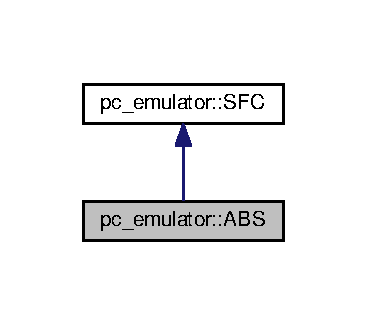
\includegraphics[width=176pt]{classpc__emulator_1_1ABS__inherit__graph}
\end{center}
\end{figure}


Collaboration diagram for pc\+\_\+emulator\+:\+:A\+BS\+:\nopagebreak
\begin{figure}[H]
\begin{center}
\leavevmode
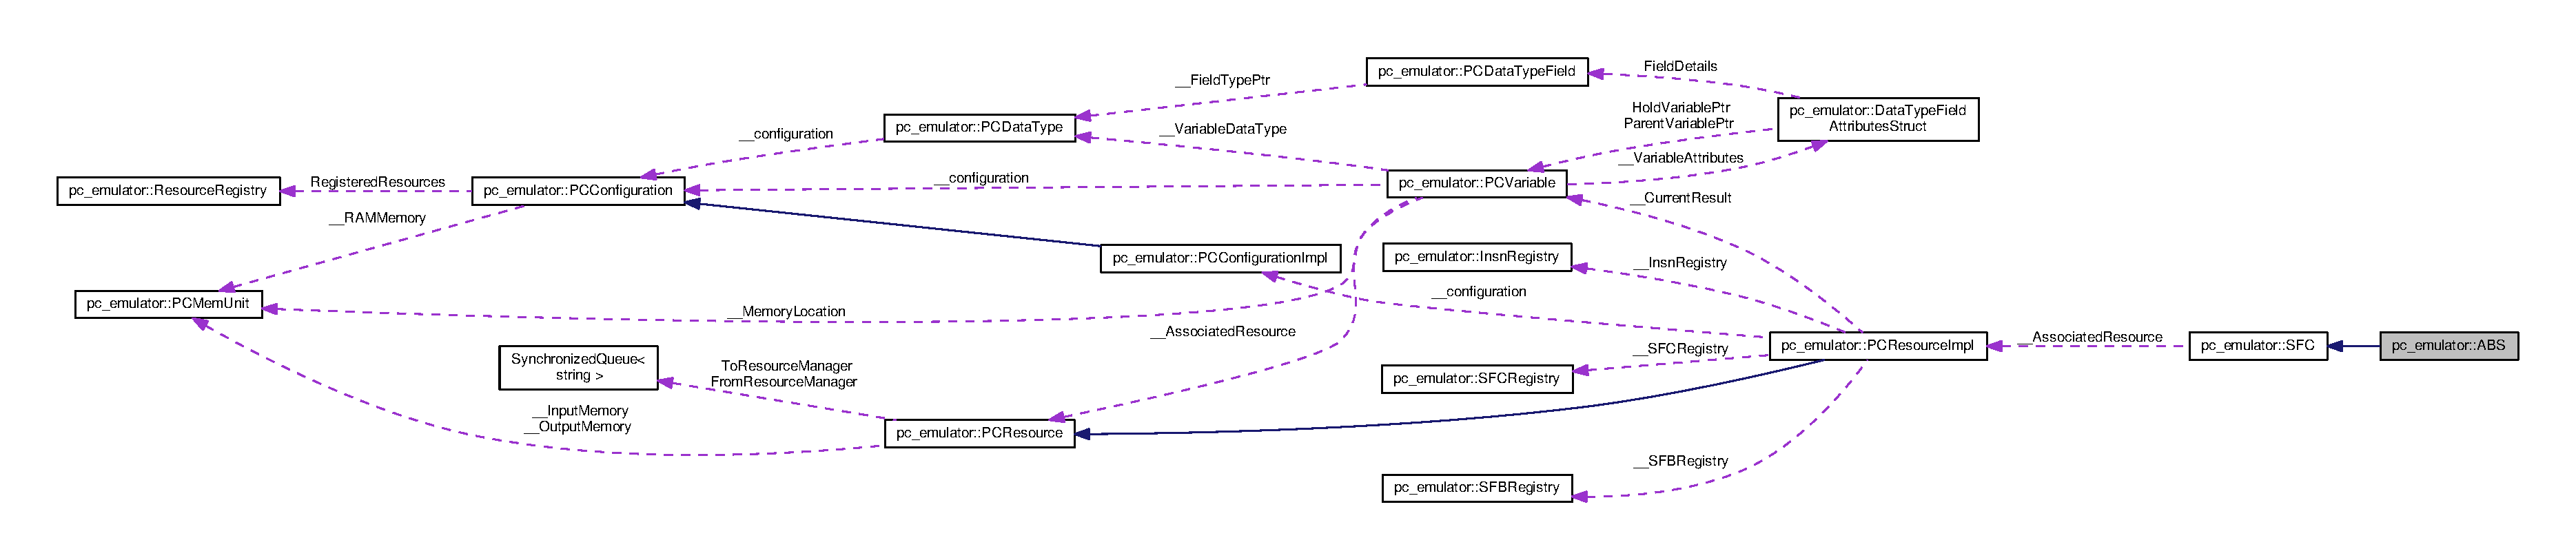
\includegraphics[width=350pt]{classpc__emulator_1_1ABS__coll__graph}
\end{center}
\end{figure}
\subsection*{Public Member Functions}
\begin{DoxyCompactItemize}
\item 
{\bfseries A\+BS} (\hyperlink{classpc__emulator_1_1PCResourceImpl}{P\+C\+Resource\+Impl} $\ast$Associated\+Resource)\hypertarget{classpc__emulator_1_1ABS_a26aec5a27db6f27894029b79b20f9359}{}\label{classpc__emulator_1_1ABS_a26aec5a27db6f27894029b79b20f9359}

\item 
void \hyperlink{classpc__emulator_1_1ABS_ac17315794160f617479e033609ed5f7c}{Execute} (\hyperlink{classpc__emulator_1_1PCVariable}{P\+C\+Variable} $\ast$Current\+Result, std\+::vector$<$ \hyperlink{classpc__emulator_1_1PCVariable}{P\+C\+Variable} $\ast$ $>$ \&Operands)
\begin{DoxyCompactList}\small\item\em Called to execute the sfc. \end{DoxyCompactList}\end{DoxyCompactItemize}
\subsection*{Additional Inherited Members}


\subsection{Detailed Description}
Definition of \hyperlink{classpc__emulator_1_1ABS}{A\+BS} \hyperlink{classpc__emulator_1_1SFC}{S\+FC}. 

\subsection{Member Function Documentation}
\index{pc\+\_\+emulator\+::\+A\+BS@{pc\+\_\+emulator\+::\+A\+BS}!Execute@{Execute}}
\index{Execute@{Execute}!pc\+\_\+emulator\+::\+A\+BS@{pc\+\_\+emulator\+::\+A\+BS}}
\subsubsection[{\texorpdfstring{Execute(\+P\+C\+Variable $\ast$\+Current\+Result, std\+::vector$<$ P\+C\+Variable $\ast$ $>$ \&\+Operands)}{Execute(PCVariable *CurrentResult, std::vector< PCVariable * > &Operands)}}]{\setlength{\rightskip}{0pt plus 5cm}void pc\+\_\+emulator\+::\+A\+B\+S\+::\+Execute (
\begin{DoxyParamCaption}
\item[{{\bf P\+C\+Variable} $\ast$}]{Current\+Result, }
\item[{std\+::vector$<$ {\bf P\+C\+Variable} $\ast$ $>$ \&}]{Operands}
\end{DoxyParamCaption}
)\hspace{0.3cm}{\ttfamily [virtual]}}\hypertarget{classpc__emulator_1_1ABS_ac17315794160f617479e033609ed5f7c}{}\label{classpc__emulator_1_1ABS_ac17315794160f617479e033609ed5f7c}


Called to execute the sfc. 


\begin{DoxyParams}{Parameters}
{\em Current\+Result} & The Current\+Result register of the task executing this \hyperlink{classpc__emulator_1_1SFC}{S\+FC} \\
\hline
{\em Operands} & Operands to the sfc \\
\hline
\end{DoxyParams}


Implements \hyperlink{classpc__emulator_1_1SFC_ab206c80fc0e429c56672b4f6a0ca8635}{pc\+\_\+emulator\+::\+S\+FC}.



The documentation for this class was generated from the following file\+:\begin{DoxyCompactItemize}
\item 
src/pc\+\_\+emulator/include/sfc/abs.\+h\end{DoxyCompactItemize}

\hypertarget{classpc__emulator_1_1ACOS}{}\section{pc\+\_\+emulator\+:\+:A\+C\+OS Class Reference}
\label{classpc__emulator_1_1ACOS}\index{pc\+\_\+emulator\+::\+A\+C\+OS@{pc\+\_\+emulator\+::\+A\+C\+OS}}


Definition of \hyperlink{classpc__emulator_1_1ACOS}{A\+C\+OS} \hyperlink{classpc__emulator_1_1SFC}{S\+FC}.  




{\ttfamily \#include $<$acos.\+h$>$}



Inheritance diagram for pc\+\_\+emulator\+:\+:A\+C\+OS\+:
\nopagebreak
\begin{figure}[H]
\begin{center}
\leavevmode
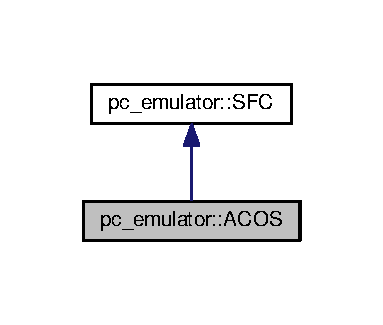
\includegraphics[width=184pt]{classpc__emulator_1_1ACOS__inherit__graph}
\end{center}
\end{figure}


Collaboration diagram for pc\+\_\+emulator\+:\+:A\+C\+OS\+:
\nopagebreak
\begin{figure}[H]
\begin{center}
\leavevmode
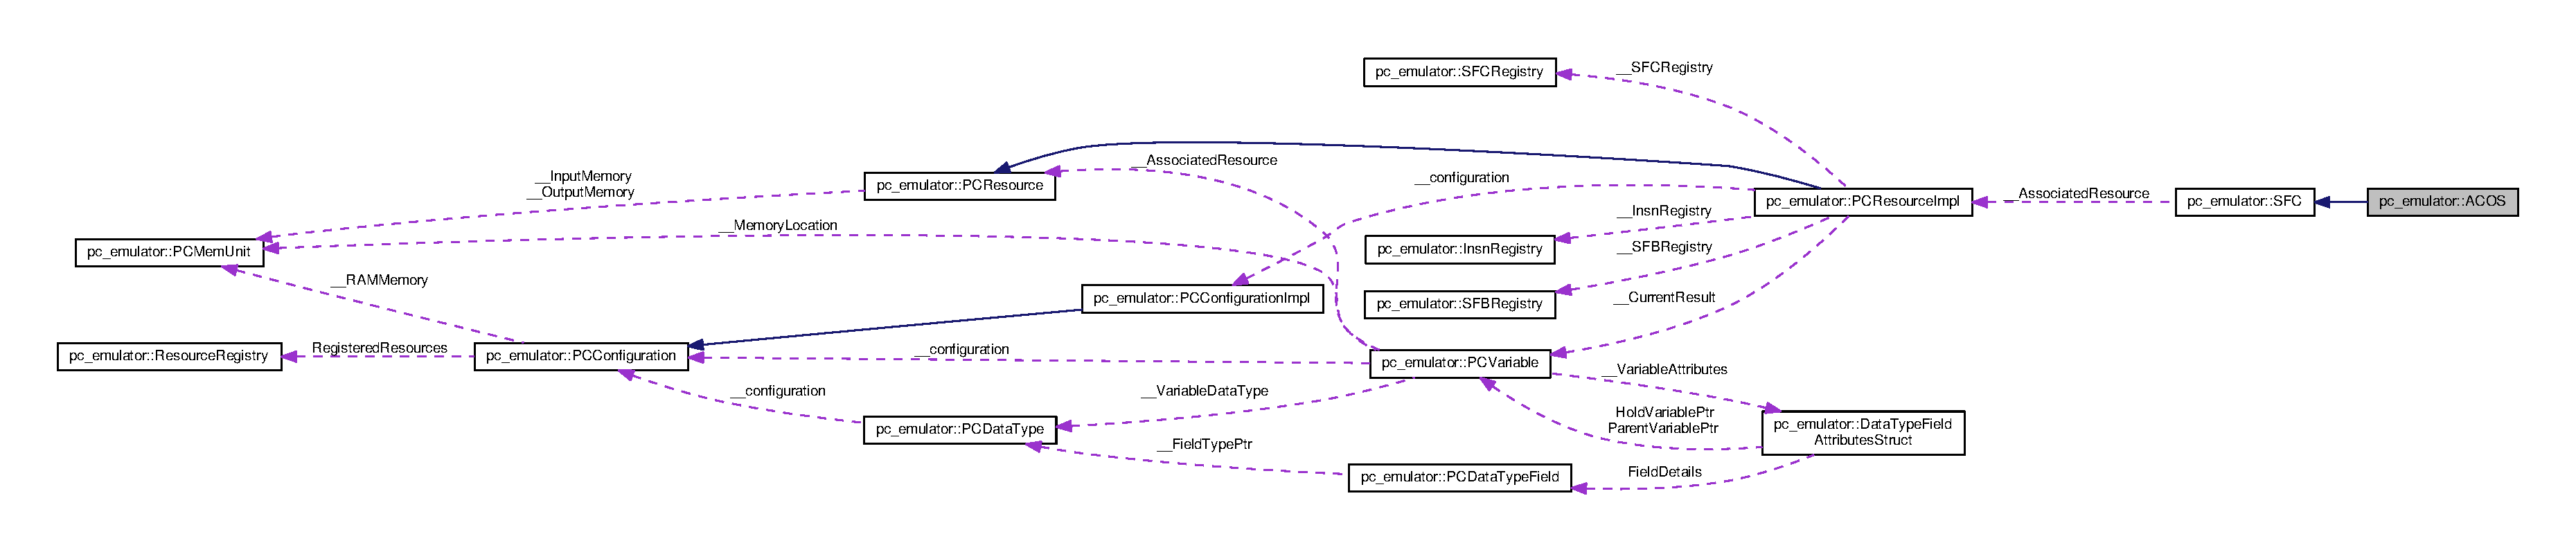
\includegraphics[width=350pt]{classpc__emulator_1_1ACOS__coll__graph}
\end{center}
\end{figure}
\subsection*{Public Member Functions}
\begin{DoxyCompactItemize}
\item 
{\bfseries A\+C\+OS} (\hyperlink{classpc__emulator_1_1PCResourceImpl}{P\+C\+Resource\+Impl} $\ast$Associated\+Resource)\hypertarget{classpc__emulator_1_1ACOS_acc35e156885aca267aa32734ccb88261}{}\label{classpc__emulator_1_1ACOS_acc35e156885aca267aa32734ccb88261}

\item 
void \hyperlink{classpc__emulator_1_1ACOS_ab1011f059918ccb28c9309f18b01cb32}{Execute} (\hyperlink{classpc__emulator_1_1PCVariable}{P\+C\+Variable} $\ast$Current\+Result, std\+::vector$<$ \hyperlink{classpc__emulator_1_1PCVariable}{P\+C\+Variable} $\ast$ $>$ \&Operands)
\begin{DoxyCompactList}\small\item\em Called to execute the sfc. \end{DoxyCompactList}\end{DoxyCompactItemize}
\subsection*{Additional Inherited Members}


\subsection{Detailed Description}
Definition of \hyperlink{classpc__emulator_1_1ACOS}{A\+C\+OS} \hyperlink{classpc__emulator_1_1SFC}{S\+FC}. 

\subsection{Member Function Documentation}
\index{pc\+\_\+emulator\+::\+A\+C\+OS@{pc\+\_\+emulator\+::\+A\+C\+OS}!Execute@{Execute}}
\index{Execute@{Execute}!pc\+\_\+emulator\+::\+A\+C\+OS@{pc\+\_\+emulator\+::\+A\+C\+OS}}
\subsubsection[{\texorpdfstring{Execute(\+P\+C\+Variable $\ast$\+Current\+Result, std\+::vector$<$ P\+C\+Variable $\ast$ $>$ \&\+Operands)}{Execute(PCVariable *CurrentResult, std::vector< PCVariable * > &Operands)}}]{\setlength{\rightskip}{0pt plus 5cm}void pc\+\_\+emulator\+::\+A\+C\+O\+S\+::\+Execute (
\begin{DoxyParamCaption}
\item[{{\bf P\+C\+Variable} $\ast$}]{Current\+Result, }
\item[{std\+::vector$<$ {\bf P\+C\+Variable} $\ast$ $>$ \&}]{Operands}
\end{DoxyParamCaption}
)\hspace{0.3cm}{\ttfamily [virtual]}}\hypertarget{classpc__emulator_1_1ACOS_ab1011f059918ccb28c9309f18b01cb32}{}\label{classpc__emulator_1_1ACOS_ab1011f059918ccb28c9309f18b01cb32}


Called to execute the sfc. 


\begin{DoxyParams}{Parameters}
{\em Current\+Result} & The Current\+Result register of the task executing this \hyperlink{classpc__emulator_1_1SFC}{S\+FC} \\
\hline
{\em Operands} & Operands to the sfc \\
\hline
\end{DoxyParams}


Implements \hyperlink{classpc__emulator_1_1SFC_ab206c80fc0e429c56672b4f6a0ca8635}{pc\+\_\+emulator\+::\+S\+FC}.



The documentation for this class was generated from the following file\+:\begin{DoxyCompactItemize}
\item 
src/pc\+\_\+emulator/include/sfc/acos.\+h\end{DoxyCompactItemize}

\hypertarget{classpc__emulator_1_1ActuatorModule}{}\section{pc\+\_\+emulator\+:\+:Actuator\+Module Class Reference}
\label{classpc__emulator_1_1ActuatorModule}\index{pc\+\_\+emulator\+::\+Actuator\+Module@{pc\+\_\+emulator\+::\+Actuator\+Module}}


Inheritance diagram for pc\+\_\+emulator\+:\+:Actuator\+Module\+:\nopagebreak
\begin{figure}[H]
\begin{center}
\leavevmode
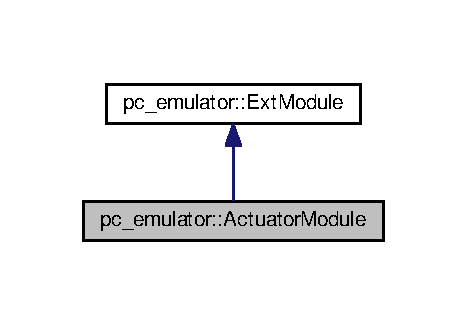
\includegraphics[width=224pt]{classpc__emulator_1_1ActuatorModule__inherit__graph}
\end{center}
\end{figure}


Collaboration diagram for pc\+\_\+emulator\+:\+:Actuator\+Module\+:\nopagebreak
\begin{figure}[H]
\begin{center}
\leavevmode
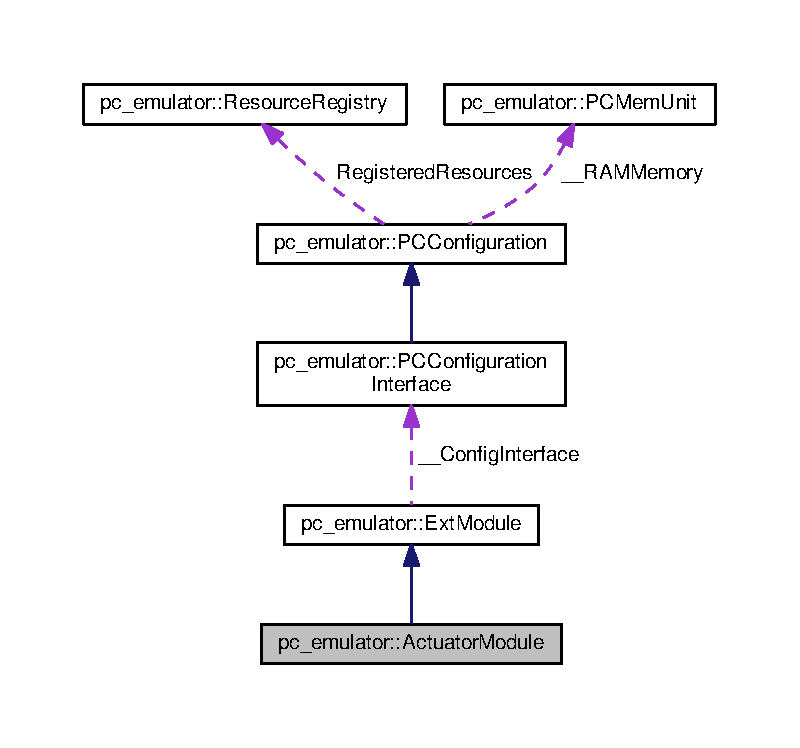
\includegraphics[width=350pt]{classpc__emulator_1_1ActuatorModule__coll__graph}
\end{center}
\end{figure}
\subsection*{Public Member Functions}
\begin{DoxyCompactItemize}
\item 
\hyperlink{classpc__emulator_1_1ActuatorModule_ab3d1a4dee9fe031b83ae6320327dc931}{Actuator\+Module} (string Configuration\+Path)\hypertarget{classpc__emulator_1_1ActuatorModule_ab3d1a4dee9fe031b83ae6320327dc931}{}\label{classpc__emulator_1_1ActuatorModule_ab3d1a4dee9fe031b83ae6320327dc931}

\begin{DoxyCompactList}\small\item\em Constructor. \end{DoxyCompactList}\item 
std\+::unique\+\_\+ptr$<$ \hyperlink{classpc__emulator_1_1PCVariableContainer}{P\+C\+Variable\+Container} $>$ \hyperlink{classpc__emulator_1_1ActuatorModule_a0708323c05eec00925ad87fe95139ce4}{Get\+Variable\+Container} (int Ram\+Byte\+Offset, int Ram\+Bit\+Offset, string Variable\+Data\+Type\+Name)
\begin{DoxyCompactList}\small\item\em N\+OT I\+M\+P\+L\+E\+M\+E\+N\+T\+ED, Actuator modules cannot query R\+AM memory. \end{DoxyCompactList}\item 
std\+::unique\+\_\+ptr$<$ \hyperlink{classpc__emulator_1_1PCVariableContainer}{P\+C\+Variable\+Container} $>$ \hyperlink{classpc__emulator_1_1ActuatorModule_a3d7f86c890cfd8301bd8481f235457d4}{Get\+Variable\+Container} (string Access\+Path)
\begin{DoxyCompactList}\small\item\em N\+OT I\+M\+P\+L\+E\+M\+E\+N\+T\+ED, Actuator modules cannot query access paths. \end{DoxyCompactList}\item 
std\+::unique\+\_\+ptr$<$ \hyperlink{classpc__emulator_1_1PCVariableContainer}{P\+C\+Variable\+Container} $>$ \hyperlink{classpc__emulator_1_1ActuatorModule_a9a11319d8be1d35f290c3172fe3f5465}{Get\+Variable\+Container} (string Resource\+Name, int Mem\+Type, int Byte\+Offset, int Bit\+Offset, string Variable\+Data\+Type\+Name)
\begin{DoxyCompactList}\small\item\em Returns a variable container for the specified resource mem location. \end{DoxyCompactList}\end{DoxyCompactItemize}
\subsection*{Additional Inherited Members}


\subsection{Member Function Documentation}
\index{pc\+\_\+emulator\+::\+Actuator\+Module@{pc\+\_\+emulator\+::\+Actuator\+Module}!Get\+Variable\+Container@{Get\+Variable\+Container}}
\index{Get\+Variable\+Container@{Get\+Variable\+Container}!pc\+\_\+emulator\+::\+Actuator\+Module@{pc\+\_\+emulator\+::\+Actuator\+Module}}
\subsubsection[{\texorpdfstring{Get\+Variable\+Container(int Ram\+Byte\+Offset, int Ram\+Bit\+Offset, string Variable\+Data\+Type\+Name)}{GetVariableContainer(int RamByteOffset, int RamBitOffset, string VariableDataTypeName)}}]{\setlength{\rightskip}{0pt plus 5cm}std\+::unique\+\_\+ptr$<${\bf P\+C\+Variable\+Container}$>$ pc\+\_\+emulator\+::\+Actuator\+Module\+::\+Get\+Variable\+Container (
\begin{DoxyParamCaption}
\item[{int}]{Ram\+Byte\+Offset, }
\item[{int}]{Ram\+Bit\+Offset, }
\item[{string}]{Variable\+Data\+Type\+Name}
\end{DoxyParamCaption}
)\hspace{0.3cm}{\ttfamily [inline]}, {\ttfamily [virtual]}}\hypertarget{classpc__emulator_1_1ActuatorModule_a0708323c05eec00925ad87fe95139ce4}{}\label{classpc__emulator_1_1ActuatorModule_a0708323c05eec00925ad87fe95139ce4}


N\+OT I\+M\+P\+L\+E\+M\+E\+N\+T\+ED, Actuator modules cannot query R\+AM memory. 

Raises an exception. 

Implements \hyperlink{classpc__emulator_1_1ExtModule_a840b25e14892e09ecca10f195cd08e6d}{pc\+\_\+emulator\+::\+Ext\+Module}.

\index{pc\+\_\+emulator\+::\+Actuator\+Module@{pc\+\_\+emulator\+::\+Actuator\+Module}!Get\+Variable\+Container@{Get\+Variable\+Container}}
\index{Get\+Variable\+Container@{Get\+Variable\+Container}!pc\+\_\+emulator\+::\+Actuator\+Module@{pc\+\_\+emulator\+::\+Actuator\+Module}}
\subsubsection[{\texorpdfstring{Get\+Variable\+Container(string Access\+Path)}{GetVariableContainer(string AccessPath)}}]{\setlength{\rightskip}{0pt plus 5cm}std\+::unique\+\_\+ptr$<${\bf P\+C\+Variable\+Container}$>$ pc\+\_\+emulator\+::\+Actuator\+Module\+::\+Get\+Variable\+Container (
\begin{DoxyParamCaption}
\item[{string}]{Access\+Path}
\end{DoxyParamCaption}
)\hspace{0.3cm}{\ttfamily [inline]}, {\ttfamily [virtual]}}\hypertarget{classpc__emulator_1_1ActuatorModule_a3d7f86c890cfd8301bd8481f235457d4}{}\label{classpc__emulator_1_1ActuatorModule_a3d7f86c890cfd8301bd8481f235457d4}


N\+OT I\+M\+P\+L\+E\+M\+E\+N\+T\+ED, Actuator modules cannot query access paths. 

Raises an exception. 

Implements \hyperlink{classpc__emulator_1_1ExtModule_a5a967d2cf1925ae2f2811892e034db14}{pc\+\_\+emulator\+::\+Ext\+Module}.

\index{pc\+\_\+emulator\+::\+Actuator\+Module@{pc\+\_\+emulator\+::\+Actuator\+Module}!Get\+Variable\+Container@{Get\+Variable\+Container}}
\index{Get\+Variable\+Container@{Get\+Variable\+Container}!pc\+\_\+emulator\+::\+Actuator\+Module@{pc\+\_\+emulator\+::\+Actuator\+Module}}
\subsubsection[{\texorpdfstring{Get\+Variable\+Container(string Resource\+Name, int Mem\+Type, int Byte\+Offset, int Bit\+Offset, string Variable\+Data\+Type\+Name)}{GetVariableContainer(string ResourceName, int MemType, int ByteOffset, int BitOffset, string VariableDataTypeName)}}]{\setlength{\rightskip}{0pt plus 5cm}std\+::unique\+\_\+ptr$<${\bf P\+C\+Variable\+Container}$>$ pc\+\_\+emulator\+::\+Actuator\+Module\+::\+Get\+Variable\+Container (
\begin{DoxyParamCaption}
\item[{string}]{Resource\+Name, }
\item[{int}]{Mem\+Type, }
\item[{int}]{Byte\+Offset, }
\item[{int}]{Bit\+Offset, }
\item[{string}]{Variable\+Data\+Type\+Name}
\end{DoxyParamCaption}
)\hspace{0.3cm}{\ttfamily [virtual]}}\hypertarget{classpc__emulator_1_1ActuatorModule_a9a11319d8be1d35f290c3172fe3f5465}{}\label{classpc__emulator_1_1ActuatorModule_a9a11319d8be1d35f290c3172fe3f5465}


Returns a variable container for the specified resource mem location. 

Raises an exception if Mem\+Type is not O\+U\+T\+P\+U\+T\+\_\+\+M\+EM 

Implements \hyperlink{classpc__emulator_1_1ExtModule_ab62dc4b158134b37e1851a79e009b194}{pc\+\_\+emulator\+::\+Ext\+Module}.



The documentation for this class was generated from the following file\+:\begin{DoxyCompactItemize}
\item 
src/pc\+\_\+emulator/ext\+\_\+modules/include/actuator\+\_\+module.\+h\end{DoxyCompactItemize}

\hypertarget{classpc__emulator_1_1ADD__Insn}{}\section{pc\+\_\+emulator\+:\+:A\+D\+D\+\_\+\+Insn Class Reference}
\label{classpc__emulator_1_1ADD__Insn}\index{pc\+\_\+emulator\+::\+A\+D\+D\+\_\+\+Insn@{pc\+\_\+emulator\+::\+A\+D\+D\+\_\+\+Insn}}


A\+DD instruction.  




{\ttfamily \#include $<$add\+\_\+insn.\+h$>$}



Inheritance diagram for pc\+\_\+emulator\+:\+:A\+D\+D\+\_\+\+Insn\+:\nopagebreak
\begin{figure}[H]
\begin{center}
\leavevmode
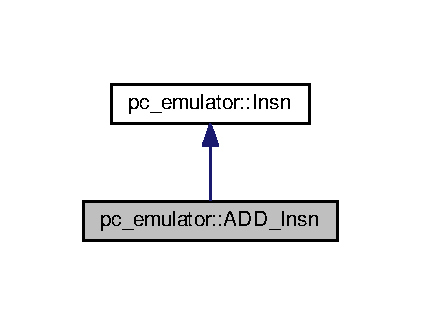
\includegraphics[width=202pt]{classpc__emulator_1_1ADD__Insn__inherit__graph}
\end{center}
\end{figure}


Collaboration diagram for pc\+\_\+emulator\+:\+:A\+D\+D\+\_\+\+Insn\+:\nopagebreak
\begin{figure}[H]
\begin{center}
\leavevmode
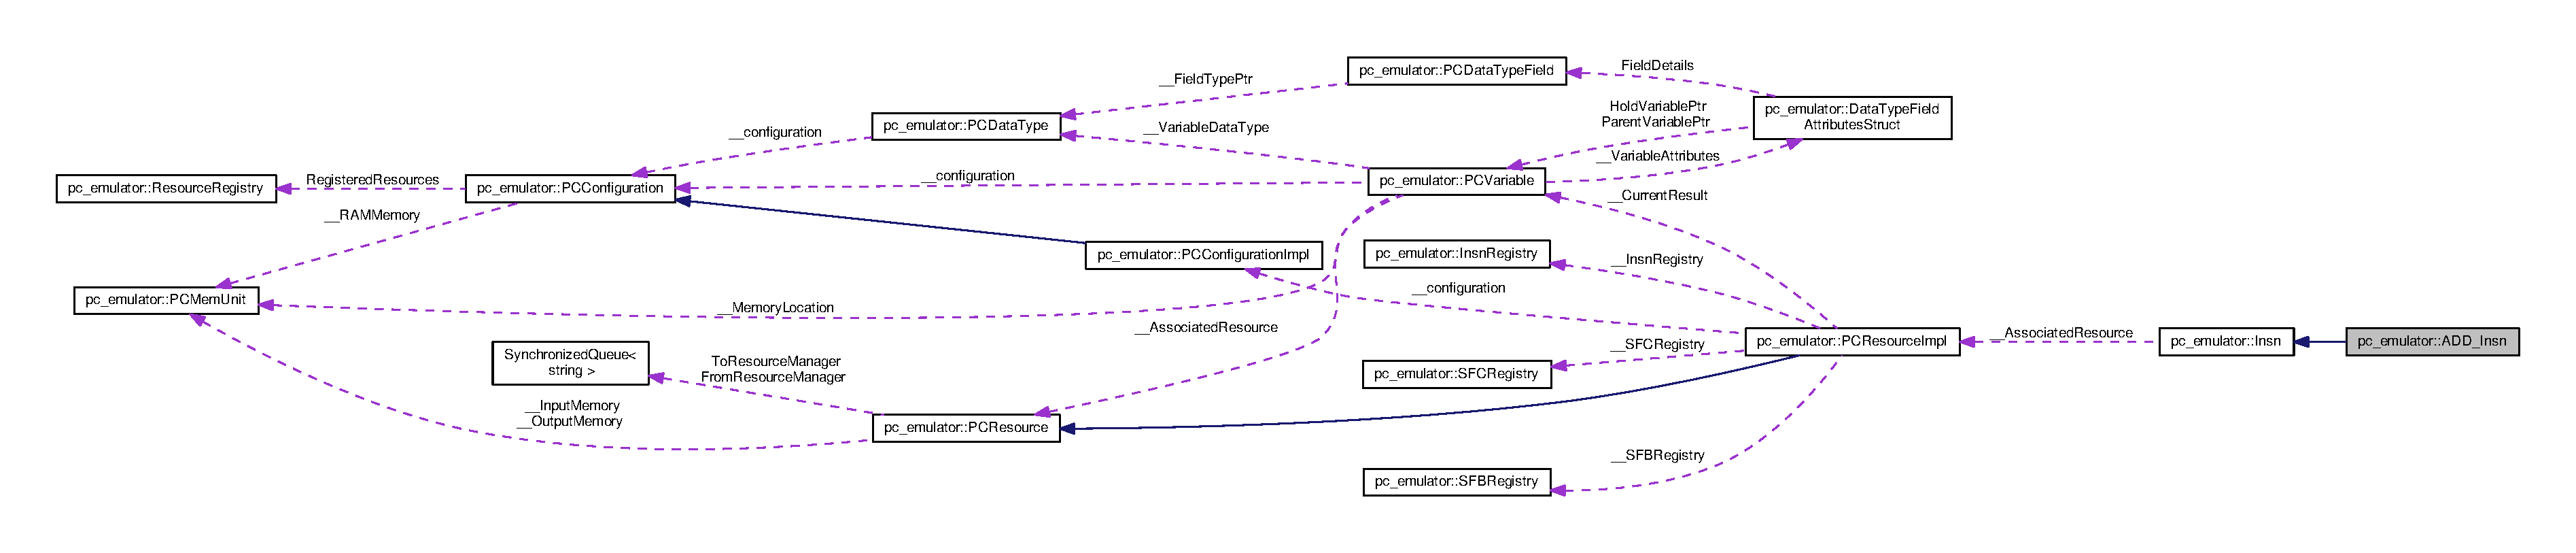
\includegraphics[width=350pt]{classpc__emulator_1_1ADD__Insn__coll__graph}
\end{center}
\end{figure}
\subsection*{Public Member Functions}
\begin{DoxyCompactItemize}
\item 
{\bfseries A\+D\+D\+\_\+\+Insn} (\hyperlink{classpc__emulator_1_1PCResourceImpl}{P\+C\+Resource\+Impl} $\ast$Associated\+Resource, bool is\+Negated)\hypertarget{classpc__emulator_1_1ADD__Insn_a644b46e66f89391369f5fe4b2e6fffd6}{}\label{classpc__emulator_1_1ADD__Insn_a644b46e66f89391369f5fe4b2e6fffd6}

\item 
void \hyperlink{classpc__emulator_1_1ADD__Insn_aebbf49265a5cc15c5ebf6d11ca4ec7c2}{Execute} (\hyperlink{classpc__emulator_1_1PCVariable}{P\+C\+Variable} $\ast$Current\+Result, std\+::vector$<$ \hyperlink{classpc__emulator_1_1PCVariable}{P\+C\+Variable} $\ast$ $>$ \&Operands)
\begin{DoxyCompactList}\small\item\em Called to execute the instruction. \end{DoxyCompactList}\end{DoxyCompactItemize}
\subsection*{Additional Inherited Members}


\subsection{Detailed Description}
A\+DD instruction. 

\subsection{Member Function Documentation}
\index{pc\+\_\+emulator\+::\+A\+D\+D\+\_\+\+Insn@{pc\+\_\+emulator\+::\+A\+D\+D\+\_\+\+Insn}!Execute@{Execute}}
\index{Execute@{Execute}!pc\+\_\+emulator\+::\+A\+D\+D\+\_\+\+Insn@{pc\+\_\+emulator\+::\+A\+D\+D\+\_\+\+Insn}}
\subsubsection[{\texorpdfstring{Execute(\+P\+C\+Variable $\ast$\+Current\+Result, std\+::vector$<$ P\+C\+Variable $\ast$ $>$ \&\+Operands)}{Execute(PCVariable *CurrentResult, std::vector< PCVariable * > &Operands)}}]{\setlength{\rightskip}{0pt plus 5cm}void pc\+\_\+emulator\+::\+A\+D\+D\+\_\+\+Insn\+::\+Execute (
\begin{DoxyParamCaption}
\item[{{\bf P\+C\+Variable} $\ast$}]{Current\+Result, }
\item[{std\+::vector$<$ {\bf P\+C\+Variable} $\ast$ $>$ \&}]{Operands}
\end{DoxyParamCaption}
)\hspace{0.3cm}{\ttfamily [virtual]}}\hypertarget{classpc__emulator_1_1ADD__Insn_aebbf49265a5cc15c5ebf6d11ca4ec7c2}{}\label{classpc__emulator_1_1ADD__Insn_aebbf49265a5cc15c5ebf6d11ca4ec7c2}


Called to execute the instruction. 


\begin{DoxyParams}{Parameters}
{\em Current\+Result} & The Current\+Result register of the task executing this \hyperlink{classpc__emulator_1_1Insn}{Insn} \\
\hline
{\em Operands} & Operands to the instruction \\
\hline
\end{DoxyParams}


Implements \hyperlink{classpc__emulator_1_1Insn_a103d27030e872a799e313df16c1f3d66}{pc\+\_\+emulator\+::\+Insn}.



The documentation for this class was generated from the following file\+:\begin{DoxyCompactItemize}
\item 
src/pc\+\_\+emulator/include/insns/add\+\_\+insn.\+h\end{DoxyCompactItemize}

\hypertarget{classpc__emulator_1_1AND__Insn}{}\section{pc\+\_\+emulator\+:\+:A\+N\+D\+\_\+\+Insn Class Reference}
\label{classpc__emulator_1_1AND__Insn}\index{pc\+\_\+emulator\+::\+A\+N\+D\+\_\+\+Insn@{pc\+\_\+emulator\+::\+A\+N\+D\+\_\+\+Insn}}


A\+ND instruction.  




{\ttfamily \#include $<$and\+\_\+insn.\+h$>$}



Inheritance diagram for pc\+\_\+emulator\+:\+:A\+N\+D\+\_\+\+Insn\+:
\nopagebreak
\begin{figure}[H]
\begin{center}
\leavevmode
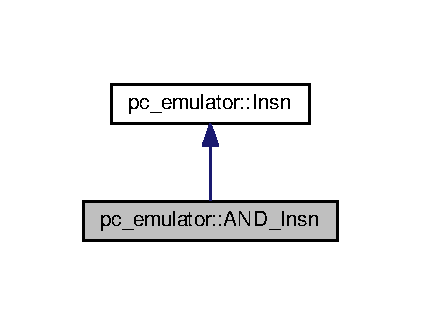
\includegraphics[width=202pt]{classpc__emulator_1_1AND__Insn__inherit__graph}
\end{center}
\end{figure}


Collaboration diagram for pc\+\_\+emulator\+:\+:A\+N\+D\+\_\+\+Insn\+:
\nopagebreak
\begin{figure}[H]
\begin{center}
\leavevmode
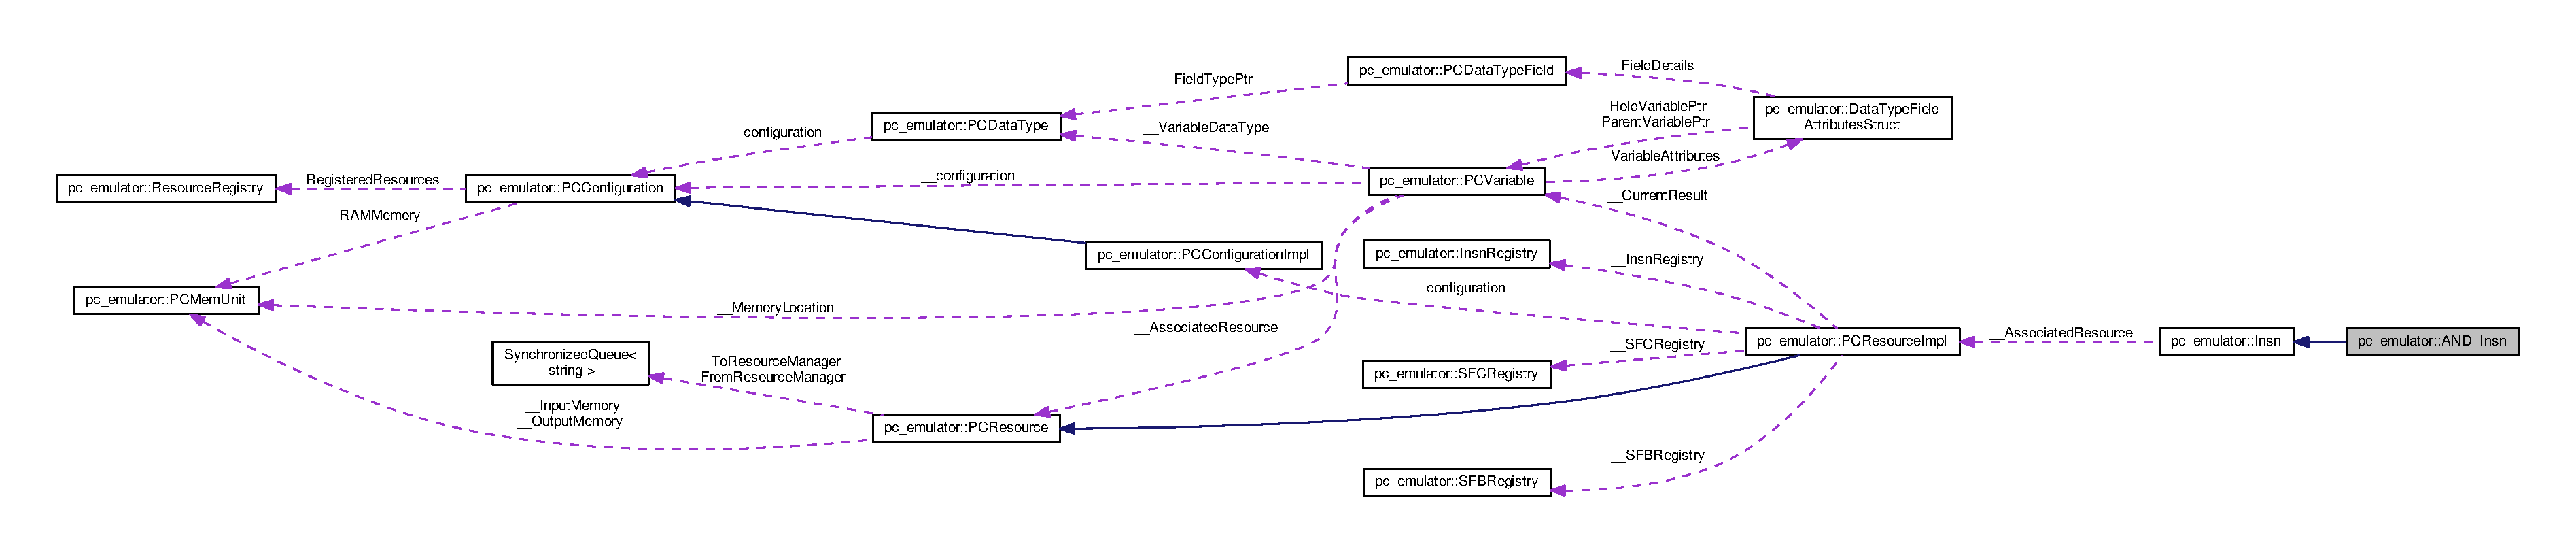
\includegraphics[width=350pt]{classpc__emulator_1_1AND__Insn__coll__graph}
\end{center}
\end{figure}
\subsection*{Public Member Functions}
\begin{DoxyCompactItemize}
\item 
{\bfseries A\+N\+D\+\_\+\+Insn} (\hyperlink{classpc__emulator_1_1PCResourceImpl}{P\+C\+Resource\+Impl} $\ast$Associated\+Resource, bool is\+Negated)\hypertarget{classpc__emulator_1_1AND__Insn_ad4020f5e9c1e89621a8253eef9be8785}{}\label{classpc__emulator_1_1AND__Insn_ad4020f5e9c1e89621a8253eef9be8785}

\item 
void \hyperlink{classpc__emulator_1_1AND__Insn_a97a9a9d54d0d91b435ce763396ec21d9}{Execute} (\hyperlink{classpc__emulator_1_1PCVariable}{P\+C\+Variable} $\ast$Current\+Result, std\+::vector$<$ \hyperlink{classpc__emulator_1_1PCVariable}{P\+C\+Variable} $\ast$ $>$ \&Operands)
\begin{DoxyCompactList}\small\item\em Called to execute the instruction. \end{DoxyCompactList}\end{DoxyCompactItemize}
\subsection*{Additional Inherited Members}


\subsection{Detailed Description}
A\+ND instruction. 

\subsection{Member Function Documentation}
\index{pc\+\_\+emulator\+::\+A\+N\+D\+\_\+\+Insn@{pc\+\_\+emulator\+::\+A\+N\+D\+\_\+\+Insn}!Execute@{Execute}}
\index{Execute@{Execute}!pc\+\_\+emulator\+::\+A\+N\+D\+\_\+\+Insn@{pc\+\_\+emulator\+::\+A\+N\+D\+\_\+\+Insn}}
\subsubsection[{\texorpdfstring{Execute(\+P\+C\+Variable $\ast$\+Current\+Result, std\+::vector$<$ P\+C\+Variable $\ast$ $>$ \&\+Operands)}{Execute(PCVariable *CurrentResult, std::vector< PCVariable * > &Operands)}}]{\setlength{\rightskip}{0pt plus 5cm}void pc\+\_\+emulator\+::\+A\+N\+D\+\_\+\+Insn\+::\+Execute (
\begin{DoxyParamCaption}
\item[{{\bf P\+C\+Variable} $\ast$}]{Current\+Result, }
\item[{std\+::vector$<$ {\bf P\+C\+Variable} $\ast$ $>$ \&}]{Operands}
\end{DoxyParamCaption}
)\hspace{0.3cm}{\ttfamily [virtual]}}\hypertarget{classpc__emulator_1_1AND__Insn_a97a9a9d54d0d91b435ce763396ec21d9}{}\label{classpc__emulator_1_1AND__Insn_a97a9a9d54d0d91b435ce763396ec21d9}


Called to execute the instruction. 


\begin{DoxyParams}{Parameters}
{\em Current\+Result} & The Current\+Result register of the task executing this \hyperlink{classpc__emulator_1_1Insn}{Insn} \\
\hline
{\em Operands} & Operands to the instruction \\
\hline
\end{DoxyParams}


Implements \hyperlink{classpc__emulator_1_1Insn_a103d27030e872a799e313df16c1f3d66}{pc\+\_\+emulator\+::\+Insn}.



The documentation for this class was generated from the following file\+:\begin{DoxyCompactItemize}
\item 
src/pc\+\_\+emulator/include/insns/and\+\_\+insn.\+h\end{DoxyCompactItemize}

\hypertarget{classpc__emulator_1_1ANY__TO__ANY}{}\section{pc\+\_\+emulator\+:\+:A\+N\+Y\+\_\+\+T\+O\+\_\+\+A\+NY Class Reference}
\label{classpc__emulator_1_1ANY__TO__ANY}\index{pc\+\_\+emulator\+::\+A\+N\+Y\+\_\+\+T\+O\+\_\+\+A\+NY@{pc\+\_\+emulator\+::\+A\+N\+Y\+\_\+\+T\+O\+\_\+\+A\+NY}}


\hyperlink{classpc__emulator_1_1ANY__TO__ANY}{A\+N\+Y\+\_\+\+T\+O\+\_\+\+A\+NY} sfc.  




{\ttfamily \#include $<$any\+\_\+to\+\_\+any.\+h$>$}



Inheritance diagram for pc\+\_\+emulator\+:\+:A\+N\+Y\+\_\+\+T\+O\+\_\+\+A\+NY\+:
\nopagebreak
\begin{figure}[H]
\begin{center}
\leavevmode
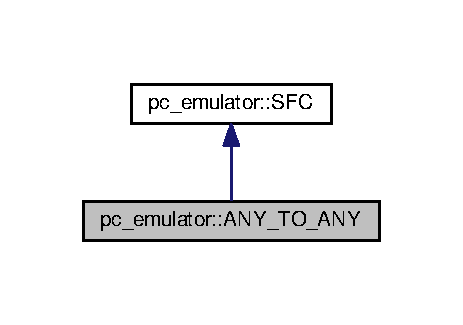
\includegraphics[width=222pt]{classpc__emulator_1_1ANY__TO__ANY__inherit__graph}
\end{center}
\end{figure}


Collaboration diagram for pc\+\_\+emulator\+:\+:A\+N\+Y\+\_\+\+T\+O\+\_\+\+A\+NY\+:
\nopagebreak
\begin{figure}[H]
\begin{center}
\leavevmode
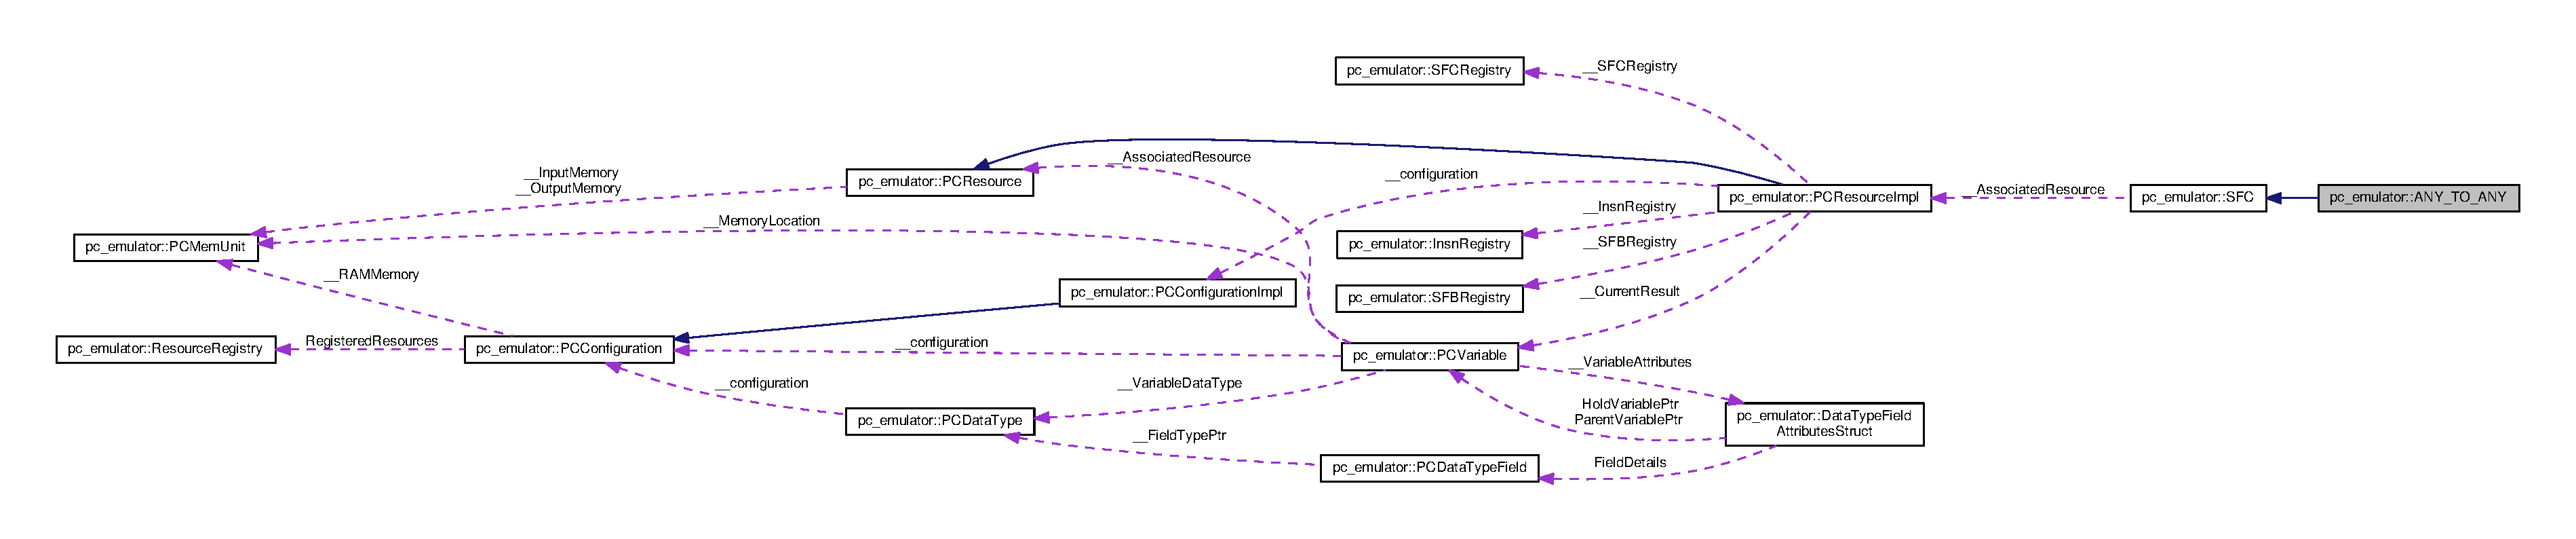
\includegraphics[width=350pt]{classpc__emulator_1_1ANY__TO__ANY__coll__graph}
\end{center}
\end{figure}
\subsection*{Public Member Functions}
\begin{DoxyCompactItemize}
\item 
{\bfseries A\+N\+Y\+\_\+\+T\+O\+\_\+\+A\+NY} (\hyperlink{classpc__emulator_1_1PCResourceImpl}{P\+C\+Resource\+Impl} $\ast$Associated\+Resource, \hyperlink{classpc__emulator_1_1PCDataType}{P\+C\+Data\+Type} $\ast$Target\+Data\+Type, \hyperlink{classpc__emulator_1_1PCDataType}{P\+C\+Data\+Type} $\ast$Src\+Data\+Type)\hypertarget{classpc__emulator_1_1ANY__TO__ANY_ad553c190c23b3d076ea749a64c8ab513}{}\label{classpc__emulator_1_1ANY__TO__ANY_ad553c190c23b3d076ea749a64c8ab513}

\item 
void \hyperlink{classpc__emulator_1_1ANY__TO__ANY_abd6bf0496fa8d85b7194024b5462a0af}{Execute} (\hyperlink{classpc__emulator_1_1PCVariable}{P\+C\+Variable} $\ast$Current\+Result, std\+::vector$<$ \hyperlink{classpc__emulator_1_1PCVariable}{P\+C\+Variable} $\ast$ $>$ \&Operands)
\begin{DoxyCompactList}\small\item\em Called to execute the sfc. \end{DoxyCompactList}\item 
\hyperlink{classpc__emulator_1_1PCVariable}{P\+C\+Variable} $\ast$ \hyperlink{classpc__emulator_1_1ANY__TO__ANY_ab1268a83de8f7107a7a997a5bf1eabe6}{Execute} (\hyperlink{classpc__emulator_1_1PCVariable}{P\+C\+Variable} $\ast$Current\+Result, \hyperlink{classpc__emulator_1_1PCVariable}{P\+C\+Variable} $\ast$Operand)
\begin{DoxyCompactList}\small\item\em Called to execute the sfc. \end{DoxyCompactList}\end{DoxyCompactItemize}
\subsection*{Additional Inherited Members}


\subsection{Detailed Description}
\hyperlink{classpc__emulator_1_1ANY__TO__ANY}{A\+N\+Y\+\_\+\+T\+O\+\_\+\+A\+NY} sfc. 

\subsection{Member Function Documentation}
\index{pc\+\_\+emulator\+::\+A\+N\+Y\+\_\+\+T\+O\+\_\+\+A\+NY@{pc\+\_\+emulator\+::\+A\+N\+Y\+\_\+\+T\+O\+\_\+\+A\+NY}!Execute@{Execute}}
\index{Execute@{Execute}!pc\+\_\+emulator\+::\+A\+N\+Y\+\_\+\+T\+O\+\_\+\+A\+NY@{pc\+\_\+emulator\+::\+A\+N\+Y\+\_\+\+T\+O\+\_\+\+A\+NY}}
\subsubsection[{\texorpdfstring{Execute(\+P\+C\+Variable $\ast$\+Current\+Result, std\+::vector$<$ P\+C\+Variable $\ast$ $>$ \&\+Operands)}{Execute(PCVariable *CurrentResult, std::vector< PCVariable * > &Operands)}}]{\setlength{\rightskip}{0pt plus 5cm}void pc\+\_\+emulator\+::\+A\+N\+Y\+\_\+\+T\+O\+\_\+\+A\+N\+Y\+::\+Execute (
\begin{DoxyParamCaption}
\item[{{\bf P\+C\+Variable} $\ast$}]{Current\+Result, }
\item[{std\+::vector$<$ {\bf P\+C\+Variable} $\ast$ $>$ \&}]{Operands}
\end{DoxyParamCaption}
)\hspace{0.3cm}{\ttfamily [virtual]}}\hypertarget{classpc__emulator_1_1ANY__TO__ANY_abd6bf0496fa8d85b7194024b5462a0af}{}\label{classpc__emulator_1_1ANY__TO__ANY_abd6bf0496fa8d85b7194024b5462a0af}


Called to execute the sfc. 


\begin{DoxyParams}{Parameters}
{\em Current\+Result} & Dummy parameter. Not used \\
\hline
{\em Operands} & Operands to the sfc \\
\hline
\end{DoxyParams}


Implements \hyperlink{classpc__emulator_1_1SFC_ab206c80fc0e429c56672b4f6a0ca8635}{pc\+\_\+emulator\+::\+S\+FC}.

\index{pc\+\_\+emulator\+::\+A\+N\+Y\+\_\+\+T\+O\+\_\+\+A\+NY@{pc\+\_\+emulator\+::\+A\+N\+Y\+\_\+\+T\+O\+\_\+\+A\+NY}!Execute@{Execute}}
\index{Execute@{Execute}!pc\+\_\+emulator\+::\+A\+N\+Y\+\_\+\+T\+O\+\_\+\+A\+NY@{pc\+\_\+emulator\+::\+A\+N\+Y\+\_\+\+T\+O\+\_\+\+A\+NY}}
\subsubsection[{\texorpdfstring{Execute(\+P\+C\+Variable $\ast$\+Current\+Result, P\+C\+Variable $\ast$\+Operand)}{Execute(PCVariable *CurrentResult, PCVariable *Operand)}}]{\setlength{\rightskip}{0pt plus 5cm}{\bf P\+C\+Variable}$\ast$ pc\+\_\+emulator\+::\+A\+N\+Y\+\_\+\+T\+O\+\_\+\+A\+N\+Y\+::\+Execute (
\begin{DoxyParamCaption}
\item[{{\bf P\+C\+Variable} $\ast$}]{Current\+Result, }
\item[{{\bf P\+C\+Variable} $\ast$}]{Operand}
\end{DoxyParamCaption}
)}\hypertarget{classpc__emulator_1_1ANY__TO__ANY_ab1268a83de8f7107a7a997a5bf1eabe6}{}\label{classpc__emulator_1_1ANY__TO__ANY_ab1268a83de8f7107a7a997a5bf1eabe6}


Called to execute the sfc. 


\begin{DoxyParams}{Parameters}
{\em Current\+Result} & Dummy parameter. Not used \\
\hline
{\em Operand} & Operand to the sfc \\
\hline
\end{DoxyParams}


The documentation for this class was generated from the following file\+:\begin{DoxyCompactItemize}
\item 
src/pc\+\_\+emulator/include/sfc/any\+\_\+to\+\_\+any.\+h\end{DoxyCompactItemize}

\hypertarget{classpc__emulator_1_1ASIN}{}\section{pc\+\_\+emulator\+:\+:A\+S\+IN Class Reference}
\label{classpc__emulator_1_1ASIN}\index{pc\+\_\+emulator\+::\+A\+S\+IN@{pc\+\_\+emulator\+::\+A\+S\+IN}}


Definition of \hyperlink{classpc__emulator_1_1ASIN}{A\+S\+IN} \hyperlink{classpc__emulator_1_1SFC}{S\+FC}.  




{\ttfamily \#include $<$asin.\+h$>$}



Inheritance diagram for pc\+\_\+emulator\+:\+:A\+S\+IN\+:
\nopagebreak
\begin{figure}[H]
\begin{center}
\leavevmode
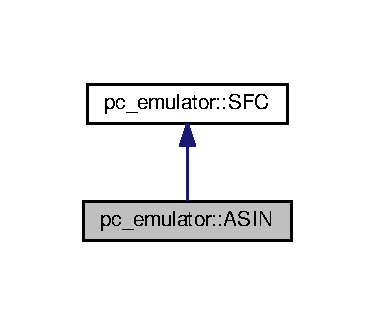
\includegraphics[width=180pt]{classpc__emulator_1_1ASIN__inherit__graph}
\end{center}
\end{figure}


Collaboration diagram for pc\+\_\+emulator\+:\+:A\+S\+IN\+:
\nopagebreak
\begin{figure}[H]
\begin{center}
\leavevmode
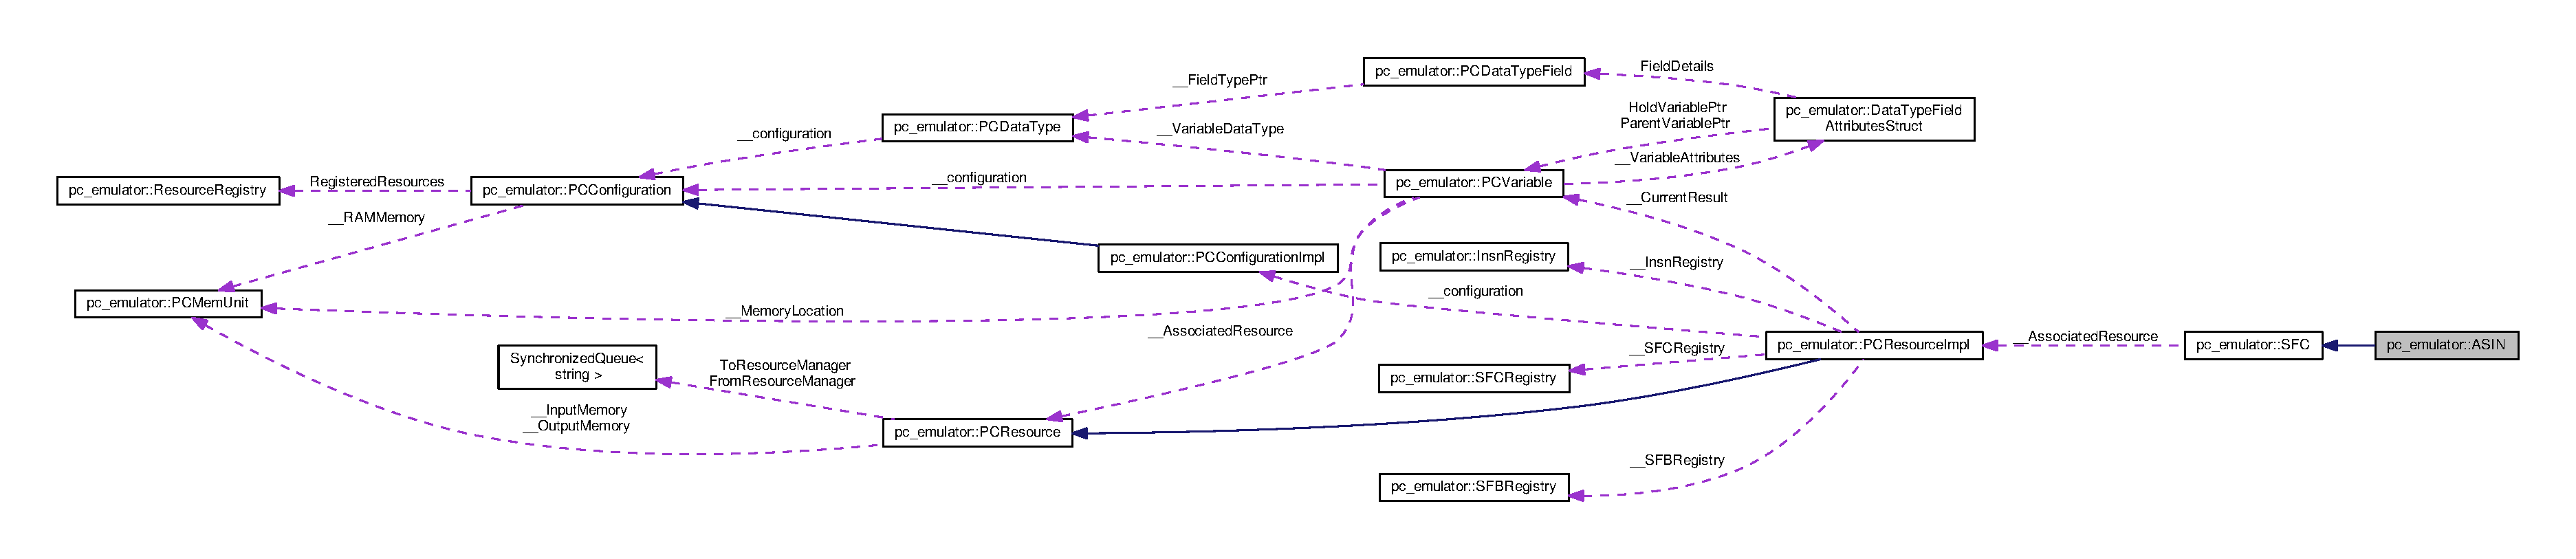
\includegraphics[width=350pt]{classpc__emulator_1_1ASIN__coll__graph}
\end{center}
\end{figure}
\subsection*{Public Member Functions}
\begin{DoxyCompactItemize}
\item 
{\bfseries A\+S\+IN} (\hyperlink{classpc__emulator_1_1PCResourceImpl}{P\+C\+Resource\+Impl} $\ast$Associated\+Resource)\hypertarget{classpc__emulator_1_1ASIN_a8721d2833b86787c29185e28b5401ed2}{}\label{classpc__emulator_1_1ASIN_a8721d2833b86787c29185e28b5401ed2}

\item 
void \hyperlink{classpc__emulator_1_1ASIN_aa2c2e179a0d54f6cf2754c7ac4c36d62}{Execute} (\hyperlink{classpc__emulator_1_1PCVariable}{P\+C\+Variable} $\ast$Current\+Result, std\+::vector$<$ \hyperlink{classpc__emulator_1_1PCVariable}{P\+C\+Variable} $\ast$ $>$ \&Operands)
\begin{DoxyCompactList}\small\item\em Called to execute the sfc. \end{DoxyCompactList}\end{DoxyCompactItemize}
\subsection*{Additional Inherited Members}


\subsection{Detailed Description}
Definition of \hyperlink{classpc__emulator_1_1ASIN}{A\+S\+IN} \hyperlink{classpc__emulator_1_1SFC}{S\+FC}. 

\subsection{Member Function Documentation}
\index{pc\+\_\+emulator\+::\+A\+S\+IN@{pc\+\_\+emulator\+::\+A\+S\+IN}!Execute@{Execute}}
\index{Execute@{Execute}!pc\+\_\+emulator\+::\+A\+S\+IN@{pc\+\_\+emulator\+::\+A\+S\+IN}}
\subsubsection[{\texorpdfstring{Execute(\+P\+C\+Variable $\ast$\+Current\+Result, std\+::vector$<$ P\+C\+Variable $\ast$ $>$ \&\+Operands)}{Execute(PCVariable *CurrentResult, std::vector< PCVariable * > &Operands)}}]{\setlength{\rightskip}{0pt plus 5cm}void pc\+\_\+emulator\+::\+A\+S\+I\+N\+::\+Execute (
\begin{DoxyParamCaption}
\item[{{\bf P\+C\+Variable} $\ast$}]{Current\+Result, }
\item[{std\+::vector$<$ {\bf P\+C\+Variable} $\ast$ $>$ \&}]{Operands}
\end{DoxyParamCaption}
)\hspace{0.3cm}{\ttfamily [virtual]}}\hypertarget{classpc__emulator_1_1ASIN_aa2c2e179a0d54f6cf2754c7ac4c36d62}{}\label{classpc__emulator_1_1ASIN_aa2c2e179a0d54f6cf2754c7ac4c36d62}


Called to execute the sfc. 


\begin{DoxyParams}{Parameters}
{\em Current\+Result} & The Current\+Result register of the task executing this \hyperlink{classpc__emulator_1_1SFC}{S\+FC} \\
\hline
{\em Operands} & Operands to the sfc \\
\hline
\end{DoxyParams}


Implements \hyperlink{classpc__emulator_1_1SFC_ab206c80fc0e429c56672b4f6a0ca8635}{pc\+\_\+emulator\+::\+S\+FC}.



The documentation for this class was generated from the following file\+:\begin{DoxyCompactItemize}
\item 
src/pc\+\_\+emulator/include/sfc/asin.\+h\end{DoxyCompactItemize}

\hypertarget{classpc__emulator_1_1ATAN}{}\section{pc\+\_\+emulator\+:\+:A\+T\+AN Class Reference}
\label{classpc__emulator_1_1ATAN}\index{pc\+\_\+emulator\+::\+A\+T\+AN@{pc\+\_\+emulator\+::\+A\+T\+AN}}


Definition of \hyperlink{classpc__emulator_1_1ATAN}{A\+T\+AN} \hyperlink{classpc__emulator_1_1SFC}{S\+FC}.  




{\ttfamily \#include $<$atan.\+h$>$}



Inheritance diagram for pc\+\_\+emulator\+:\+:A\+T\+AN\+:\nopagebreak
\begin{figure}[H]
\begin{center}
\leavevmode
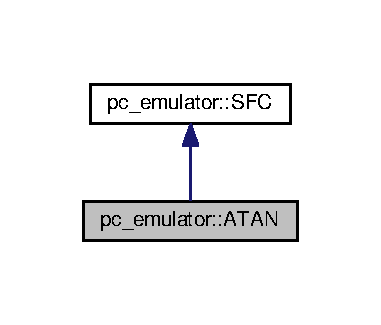
\includegraphics[width=183pt]{classpc__emulator_1_1ATAN__inherit__graph}
\end{center}
\end{figure}


Collaboration diagram for pc\+\_\+emulator\+:\+:A\+T\+AN\+:\nopagebreak
\begin{figure}[H]
\begin{center}
\leavevmode
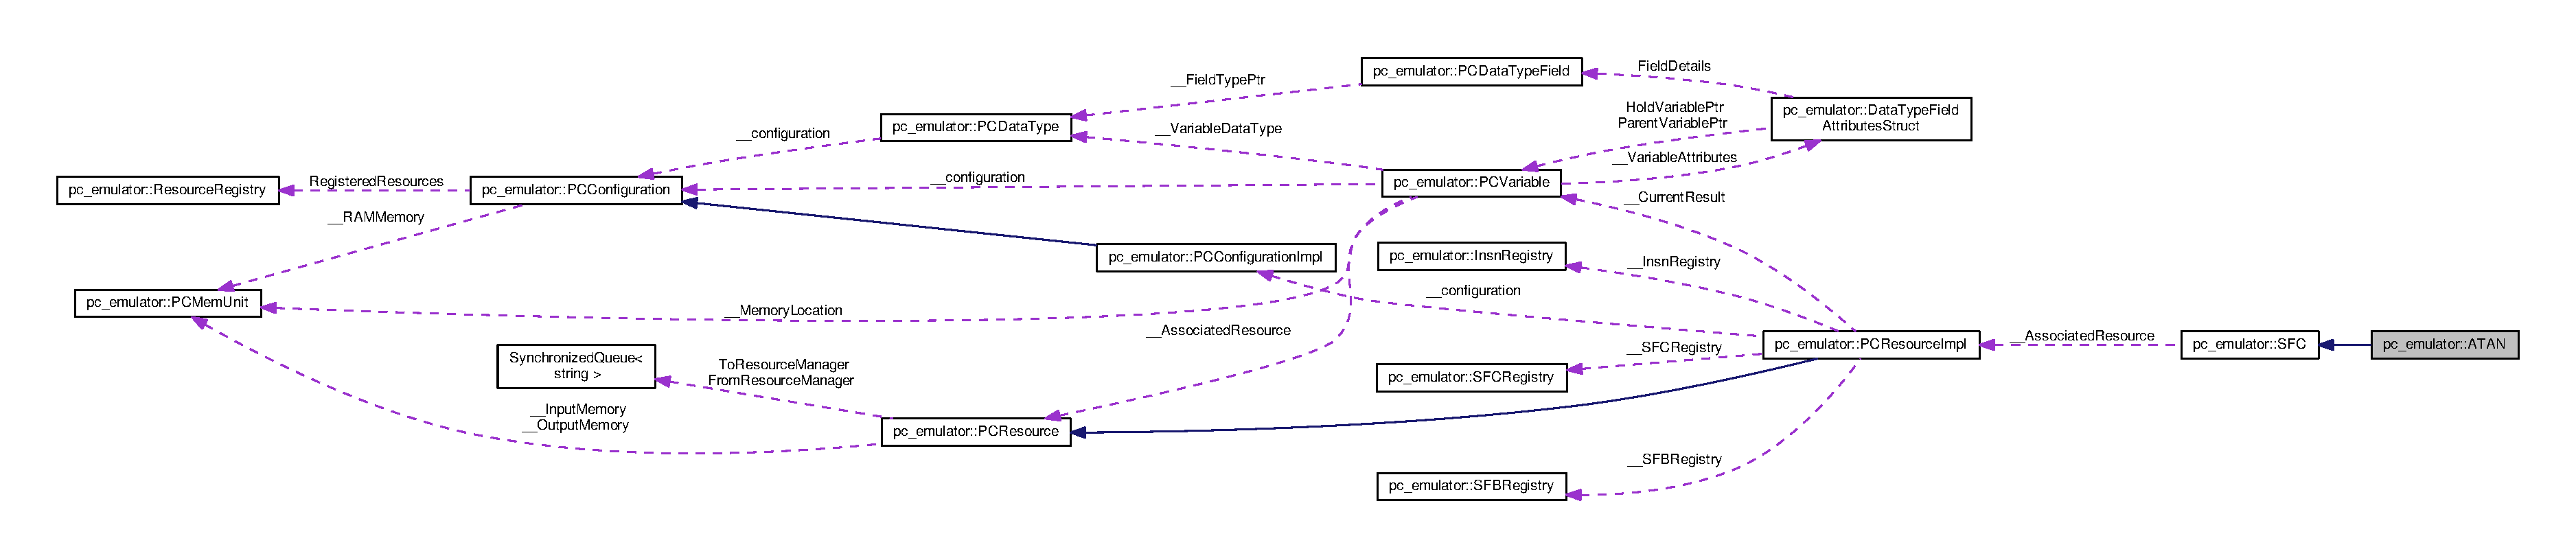
\includegraphics[width=350pt]{classpc__emulator_1_1ATAN__coll__graph}
\end{center}
\end{figure}
\subsection*{Public Member Functions}
\begin{DoxyCompactItemize}
\item 
{\bfseries A\+T\+AN} (\hyperlink{classpc__emulator_1_1PCResourceImpl}{P\+C\+Resource\+Impl} $\ast$Associated\+Resource)\hypertarget{classpc__emulator_1_1ATAN_a93a3fa1e2c52e61cababde13e15bafe3}{}\label{classpc__emulator_1_1ATAN_a93a3fa1e2c52e61cababde13e15bafe3}

\item 
void \hyperlink{classpc__emulator_1_1ATAN_a67a62838992aa4ccca28250a8f5b9a81}{Execute} (\hyperlink{classpc__emulator_1_1PCVariable}{P\+C\+Variable} $\ast$Current\+Result, std\+::vector$<$ \hyperlink{classpc__emulator_1_1PCVariable}{P\+C\+Variable} $\ast$ $>$ \&Operands)
\begin{DoxyCompactList}\small\item\em Called to execute the sfc. \end{DoxyCompactList}\end{DoxyCompactItemize}
\subsection*{Additional Inherited Members}


\subsection{Detailed Description}
Definition of \hyperlink{classpc__emulator_1_1ATAN}{A\+T\+AN} \hyperlink{classpc__emulator_1_1SFC}{S\+FC}. 

\subsection{Member Function Documentation}
\index{pc\+\_\+emulator\+::\+A\+T\+AN@{pc\+\_\+emulator\+::\+A\+T\+AN}!Execute@{Execute}}
\index{Execute@{Execute}!pc\+\_\+emulator\+::\+A\+T\+AN@{pc\+\_\+emulator\+::\+A\+T\+AN}}
\subsubsection[{\texorpdfstring{Execute(\+P\+C\+Variable $\ast$\+Current\+Result, std\+::vector$<$ P\+C\+Variable $\ast$ $>$ \&\+Operands)}{Execute(PCVariable *CurrentResult, std::vector< PCVariable * > &Operands)}}]{\setlength{\rightskip}{0pt plus 5cm}void pc\+\_\+emulator\+::\+A\+T\+A\+N\+::\+Execute (
\begin{DoxyParamCaption}
\item[{{\bf P\+C\+Variable} $\ast$}]{Current\+Result, }
\item[{std\+::vector$<$ {\bf P\+C\+Variable} $\ast$ $>$ \&}]{Operands}
\end{DoxyParamCaption}
)\hspace{0.3cm}{\ttfamily [virtual]}}\hypertarget{classpc__emulator_1_1ATAN_a67a62838992aa4ccca28250a8f5b9a81}{}\label{classpc__emulator_1_1ATAN_a67a62838992aa4ccca28250a8f5b9a81}


Called to execute the sfc. 


\begin{DoxyParams}{Parameters}
{\em Current\+Result} & The Current\+Result register of the task executing this \hyperlink{classpc__emulator_1_1SFC}{S\+FC} \\
\hline
{\em Operands} & Operands to the sfc \\
\hline
\end{DoxyParams}


Implements \hyperlink{classpc__emulator_1_1SFC_ab206c80fc0e429c56672b4f6a0ca8635}{pc\+\_\+emulator\+::\+S\+FC}.



The documentation for this class was generated from the following file\+:\begin{DoxyCompactItemize}
\item 
src/pc\+\_\+emulator/include/sfc/atan.\+h\end{DoxyCompactItemize}

\hypertarget{classpc__emulator_1_1Clock}{}\section{pc\+\_\+emulator\+:\+:Clock Class Reference}
\label{classpc__emulator_1_1Clock}\index{pc\+\_\+emulator\+::\+Clock@{pc\+\_\+emulator\+::\+Clock}}


\hyperlink{classpc__emulator_1_1Clock}{Clock} associated with a resource.  




{\ttfamily \#include $<$pc\+\_\+clock.\+h$>$}



Collaboration diagram for pc\+\_\+emulator\+:\+:Clock\+:
\nopagebreak
\begin{figure}[H]
\begin{center}
\leavevmode
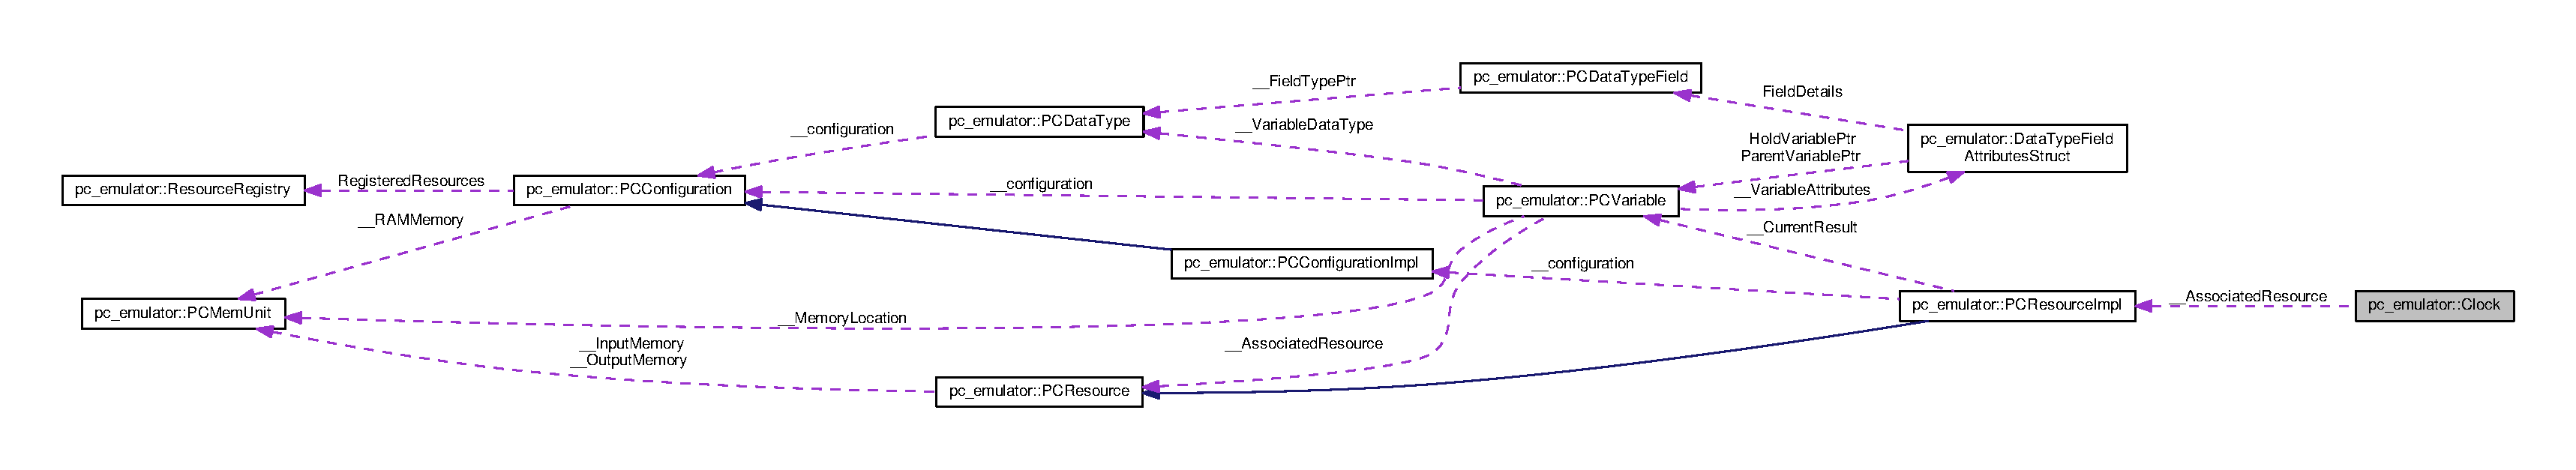
\includegraphics[width=350pt]{classpc__emulator_1_1Clock__coll__graph}
\end{center}
\end{figure}
\subsection*{Public Member Functions}
\begin{DoxyCompactItemize}
\item 
\hyperlink{classpc__emulator_1_1Clock_a512ea6e88d7df5ac3658cfb7e2206a3b}{Clock} (bool is\+\_\+virtual, \hyperlink{classpc__emulator_1_1PCResourceImpl}{P\+C\+Resource\+Impl} $\ast$Associated\+Resource)\hypertarget{classpc__emulator_1_1Clock_a512ea6e88d7df5ac3658cfb7e2206a3b}{}\label{classpc__emulator_1_1Clock_a512ea6e88d7df5ac3658cfb7e2206a3b}

\begin{DoxyCompactList}\small\item\em Constructor. \end{DoxyCompactList}\item 
double \hyperlink{classpc__emulator_1_1Clock_a17eec248287f3b57b699eea5b5a8e43f}{Get\+Current\+Time} ()\hypertarget{classpc__emulator_1_1Clock_a17eec248287f3b57b699eea5b5a8e43f}{}\label{classpc__emulator_1_1Clock_a17eec248287f3b57b699eea5b5a8e43f}

\begin{DoxyCompactList}\small\item\em Returns current time. \end{DoxyCompactList}\item 
void \hyperlink{classpc__emulator_1_1Clock_a4c54d7f36d90db5ddae81fca94d835c9}{Update\+Current\+Time} (double inc\+\_\+amount)\hypertarget{classpc__emulator_1_1Clock_a4c54d7f36d90db5ddae81fca94d835c9}{}\label{classpc__emulator_1_1Clock_a4c54d7f36d90db5ddae81fca94d835c9}

\begin{DoxyCompactList}\small\item\em Increments current time by the specifiede amount. \end{DoxyCompactList}\item 
void \hyperlink{classpc__emulator_1_1Clock_afab6f601e53dab4ef79792e4e57d5247}{Sleep\+For} (int sleep\+\_\+duration\+\_\+us)\hypertarget{classpc__emulator_1_1Clock_afab6f601e53dab4ef79792e4e57d5247}{}\label{classpc__emulator_1_1Clock_afab6f601e53dab4ef79792e4e57d5247}

\begin{DoxyCompactList}\small\item\em Sleep for specified duration in microseconds. \end{DoxyCompactList}\end{DoxyCompactItemize}
\subsection*{Public Attributes}
\begin{DoxyCompactItemize}
\item 
double \hyperlink{classpc__emulator_1_1Clock_ad9198c0f45039a5b22c1404bdd245679}{\+\_\+\+\_\+time}
\item 
bool \hyperlink{classpc__emulator_1_1Clock_a0f6af10c0d261885b85149902e273725}{\+\_\+\+\_\+is\+\_\+virtual}
\item 
double {\bfseries \+\_\+\+\_\+expected\+\_\+time}\hypertarget{classpc__emulator_1_1Clock_a7adf6bf1c1ad60171c37fc2e86932b12}{}\label{classpc__emulator_1_1Clock_a7adf6bf1c1ad60171c37fc2e86932b12}

\item 
\hyperlink{classpc__emulator_1_1PCResourceImpl}{P\+C\+Resource\+Impl} $\ast$ \hyperlink{classpc__emulator_1_1Clock_aba91d4760a2681b29264c021b519b10b}{\+\_\+\+\_\+\+Associated\+Resource}
\end{DoxyCompactItemize}


\subsection{Detailed Description}
\hyperlink{classpc__emulator_1_1Clock}{Clock} associated with a resource. 

\subsection{Member Data Documentation}
\index{pc\+\_\+emulator\+::\+Clock@{pc\+\_\+emulator\+::\+Clock}!\+\_\+\+\_\+\+Associated\+Resource@{\+\_\+\+\_\+\+Associated\+Resource}}
\index{\+\_\+\+\_\+\+Associated\+Resource@{\+\_\+\+\_\+\+Associated\+Resource}!pc\+\_\+emulator\+::\+Clock@{pc\+\_\+emulator\+::\+Clock}}
\subsubsection[{\texorpdfstring{\+\_\+\+\_\+\+Associated\+Resource}{__AssociatedResource}}]{\setlength{\rightskip}{0pt plus 5cm}{\bf P\+C\+Resource\+Impl}$\ast$ pc\+\_\+emulator\+::\+Clock\+::\+\_\+\+\_\+\+Associated\+Resource}\hypertarget{classpc__emulator_1_1Clock_aba91d4760a2681b29264c021b519b10b}{}\label{classpc__emulator_1_1Clock_aba91d4760a2681b29264c021b519b10b}
Associated Resource \index{pc\+\_\+emulator\+::\+Clock@{pc\+\_\+emulator\+::\+Clock}!\+\_\+\+\_\+is\+\_\+virtual@{\+\_\+\+\_\+is\+\_\+virtual}}
\index{\+\_\+\+\_\+is\+\_\+virtual@{\+\_\+\+\_\+is\+\_\+virtual}!pc\+\_\+emulator\+::\+Clock@{pc\+\_\+emulator\+::\+Clock}}
\subsubsection[{\texorpdfstring{\+\_\+\+\_\+is\+\_\+virtual}{__is_virtual}}]{\setlength{\rightskip}{0pt plus 5cm}bool pc\+\_\+emulator\+::\+Clock\+::\+\_\+\+\_\+is\+\_\+virtual}\hypertarget{classpc__emulator_1_1Clock_a0f6af10c0d261885b85149902e273725}{}\label{classpc__emulator_1_1Clock_a0f6af10c0d261885b85149902e273725}
Is clock virtual ? \index{pc\+\_\+emulator\+::\+Clock@{pc\+\_\+emulator\+::\+Clock}!\+\_\+\+\_\+time@{\+\_\+\+\_\+time}}
\index{\+\_\+\+\_\+time@{\+\_\+\+\_\+time}!pc\+\_\+emulator\+::\+Clock@{pc\+\_\+emulator\+::\+Clock}}
\subsubsection[{\texorpdfstring{\+\_\+\+\_\+time}{__time}}]{\setlength{\rightskip}{0pt plus 5cm}double pc\+\_\+emulator\+::\+Clock\+::\+\_\+\+\_\+time}\hypertarget{classpc__emulator_1_1Clock_ad9198c0f45039a5b22c1404bdd245679}{}\label{classpc__emulator_1_1Clock_ad9198c0f45039a5b22c1404bdd245679}
Current time 

The documentation for this class was generated from the following file\+:\begin{DoxyCompactItemize}
\item 
src/pc\+\_\+emulator/include/pc\+\_\+clock.\+h\end{DoxyCompactItemize}

\hypertarget{classpc__emulator_1_1CommModule}{}\section{pc\+\_\+emulator\+:\+:Comm\+Module Class Reference}
\label{classpc__emulator_1_1CommModule}\index{pc\+\_\+emulator\+::\+Comm\+Module@{pc\+\_\+emulator\+::\+Comm\+Module}}


Inheritance diagram for pc\+\_\+emulator\+:\+:Comm\+Module\+:
\nopagebreak
\begin{figure}[H]
\begin{center}
\leavevmode
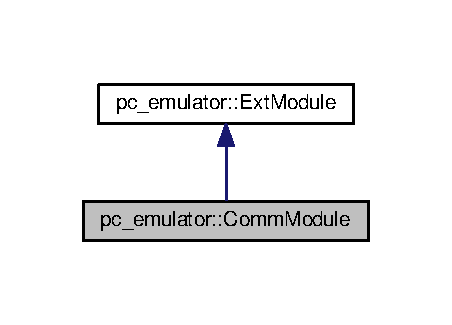
\includegraphics[width=217pt]{classpc__emulator_1_1CommModule__inherit__graph}
\end{center}
\end{figure}


Collaboration diagram for pc\+\_\+emulator\+:\+:Comm\+Module\+:
\nopagebreak
\begin{figure}[H]
\begin{center}
\leavevmode
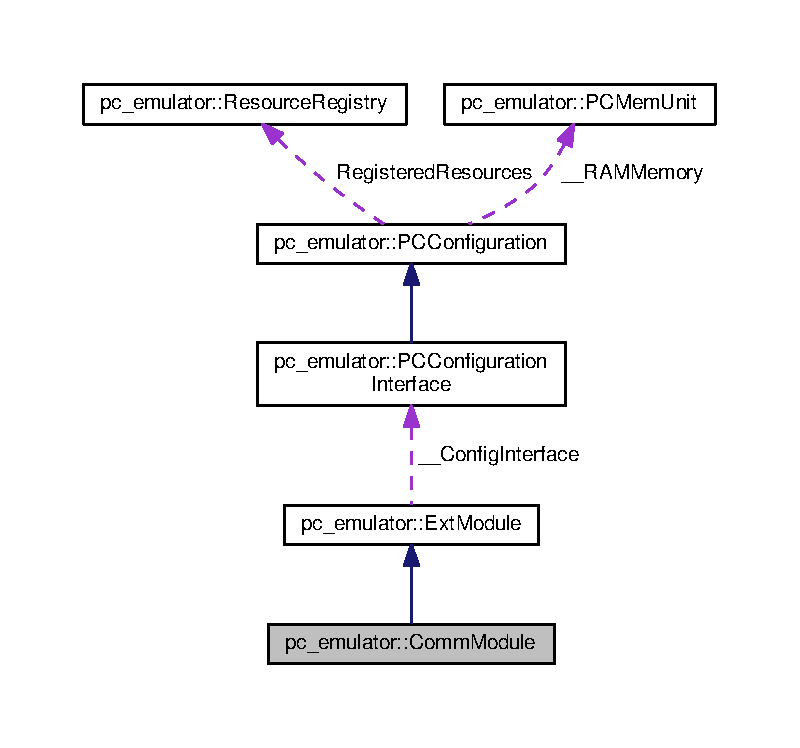
\includegraphics[width=350pt]{classpc__emulator_1_1CommModule__coll__graph}
\end{center}
\end{figure}
\subsection*{Public Member Functions}
\begin{DoxyCompactItemize}
\item 
\hyperlink{classpc__emulator_1_1CommModule_abddc1be92ad188b1177a6e32f95a81b2}{Comm\+Module} (string Configuration\+Path)\hypertarget{classpc__emulator_1_1CommModule_abddc1be92ad188b1177a6e32f95a81b2}{}\label{classpc__emulator_1_1CommModule_abddc1be92ad188b1177a6e32f95a81b2}

\begin{DoxyCompactList}\small\item\em Constructoe. \end{DoxyCompactList}\item 
std\+::unique\+\_\+ptr$<$ \hyperlink{classpc__emulator_1_1PCVariableContainer}{P\+C\+Variable\+Container} $>$ \hyperlink{classpc__emulator_1_1CommModule_a674b8ae9e9655c59be67ebd05f66107d}{Get\+Variable\+Container} (int Ram\+Byte\+Offset, int Ram\+Bit\+Offset, string Variable\+Data\+Type\+Name)
\begin{DoxyCompactList}\small\item\em Communication modules can create variables pointing to addresses. \end{DoxyCompactList}\item 
std\+::unique\+\_\+ptr$<$ \hyperlink{classpc__emulator_1_1PCVariableContainer}{P\+C\+Variable\+Container} $>$ \hyperlink{classpc__emulator_1_1CommModule_af99e6d65047aae685e4292814f85c33b}{Get\+Variable\+Container} (string Resource\+Name, int Mem\+Type, int Byte\+Offset, int Bit\+Offset, string Variable\+Data\+Type\+Name)
\begin{DoxyCompactList}\small\item\em N\+OT I\+M\+P\+L\+E\+M\+E\+N\+T\+ED, Communication modules can only query access paths/\+R\+AM. \end{DoxyCompactList}\item 
std\+::unique\+\_\+ptr$<$ \hyperlink{classpc__emulator_1_1PCVariableContainer}{P\+C\+Variable\+Container} $>$ \hyperlink{classpc__emulator_1_1CommModule_a1643e230094b1ffbcaedcfa1de0f8bc8}{Get\+Variable\+Container} (string Nested\+Access\+Path)
\begin{DoxyCompactList}\small\item\em Returns a variable container for a given nested access path. \end{DoxyCompactList}\end{DoxyCompactItemize}
\subsection*{Additional Inherited Members}


\subsection{Member Function Documentation}
\index{pc\+\_\+emulator\+::\+Comm\+Module@{pc\+\_\+emulator\+::\+Comm\+Module}!Get\+Variable\+Container@{Get\+Variable\+Container}}
\index{Get\+Variable\+Container@{Get\+Variable\+Container}!pc\+\_\+emulator\+::\+Comm\+Module@{pc\+\_\+emulator\+::\+Comm\+Module}}
\subsubsection[{\texorpdfstring{Get\+Variable\+Container(int Ram\+Byte\+Offset, int Ram\+Bit\+Offset, string Variable\+Data\+Type\+Name)}{GetVariableContainer(int RamByteOffset, int RamBitOffset, string VariableDataTypeName)}}]{\setlength{\rightskip}{0pt plus 5cm}std\+::unique\+\_\+ptr$<${\bf P\+C\+Variable\+Container}$>$ pc\+\_\+emulator\+::\+Comm\+Module\+::\+Get\+Variable\+Container (
\begin{DoxyParamCaption}
\item[{int}]{Ram\+Byte\+Offset, }
\item[{int}]{Ram\+Bit\+Offset, }
\item[{string}]{Variable\+Data\+Type\+Name}
\end{DoxyParamCaption}
)\hspace{0.3cm}{\ttfamily [virtual]}}\hypertarget{classpc__emulator_1_1CommModule_a674b8ae9e9655c59be67ebd05f66107d}{}\label{classpc__emulator_1_1CommModule_a674b8ae9e9655c59be67ebd05f66107d}


Communication modules can create variables pointing to addresses. 


\begin{DoxyParams}{Parameters}
{\em Ram\+Byte\+Offset} & starting byte offset within the R\+AM \\
\hline
{\em Ram\+Bit\+Offset} & starting bit offset within the chosen byte \\
\hline
{\em Variable\+Data\+Type\+Name} & The specified address is initialized with a pointer of this type \\
\hline
\end{DoxyParams}
\begin{DoxyReturn}{Returns}
\hyperlink{classpc__emulator_1_1PCVariableContainer}{P\+C\+Variable\+Container} which is defined over the specified R\+AM location and initialized to the specified data type 
\end{DoxyReturn}


Implements \hyperlink{classpc__emulator_1_1ExtModule_a840b25e14892e09ecca10f195cd08e6d}{pc\+\_\+emulator\+::\+Ext\+Module}.

\index{pc\+\_\+emulator\+::\+Comm\+Module@{pc\+\_\+emulator\+::\+Comm\+Module}!Get\+Variable\+Container@{Get\+Variable\+Container}}
\index{Get\+Variable\+Container@{Get\+Variable\+Container}!pc\+\_\+emulator\+::\+Comm\+Module@{pc\+\_\+emulator\+::\+Comm\+Module}}
\subsubsection[{\texorpdfstring{Get\+Variable\+Container(string Resource\+Name, int Mem\+Type, int Byte\+Offset, int Bit\+Offset, string Variable\+Data\+Type\+Name)}{GetVariableContainer(string ResourceName, int MemType, int ByteOffset, int BitOffset, string VariableDataTypeName)}}]{\setlength{\rightskip}{0pt plus 5cm}std\+::unique\+\_\+ptr$<${\bf P\+C\+Variable\+Container}$>$ pc\+\_\+emulator\+::\+Comm\+Module\+::\+Get\+Variable\+Container (
\begin{DoxyParamCaption}
\item[{string}]{Resource\+Name, }
\item[{int}]{Mem\+Type, }
\item[{int}]{Byte\+Offset, }
\item[{int}]{Bit\+Offset, }
\item[{string}]{Variable\+Data\+Type\+Name}
\end{DoxyParamCaption}
)\hspace{0.3cm}{\ttfamily [inline]}, {\ttfamily [virtual]}}\hypertarget{classpc__emulator_1_1CommModule_af99e6d65047aae685e4292814f85c33b}{}\label{classpc__emulator_1_1CommModule_af99e6d65047aae685e4292814f85c33b}


N\+OT I\+M\+P\+L\+E\+M\+E\+N\+T\+ED, Communication modules can only query access paths/\+R\+AM. 

Raises an exception. 

Implements \hyperlink{classpc__emulator_1_1ExtModule_ab62dc4b158134b37e1851a79e009b194}{pc\+\_\+emulator\+::\+Ext\+Module}.

\index{pc\+\_\+emulator\+::\+Comm\+Module@{pc\+\_\+emulator\+::\+Comm\+Module}!Get\+Variable\+Container@{Get\+Variable\+Container}}
\index{Get\+Variable\+Container@{Get\+Variable\+Container}!pc\+\_\+emulator\+::\+Comm\+Module@{pc\+\_\+emulator\+::\+Comm\+Module}}
\subsubsection[{\texorpdfstring{Get\+Variable\+Container(string Nested\+Access\+Path)}{GetVariableContainer(string NestedAccessPath)}}]{\setlength{\rightskip}{0pt plus 5cm}std\+::unique\+\_\+ptr$<${\bf P\+C\+Variable\+Container}$>$ pc\+\_\+emulator\+::\+Comm\+Module\+::\+Get\+Variable\+Container (
\begin{DoxyParamCaption}
\item[{string}]{Nested\+Access\+Path}
\end{DoxyParamCaption}
)\hspace{0.3cm}{\ttfamily [virtual]}}\hypertarget{classpc__emulator_1_1CommModule_a1643e230094b1ffbcaedcfa1de0f8bc8}{}\label{classpc__emulator_1_1CommModule_a1643e230094b1ffbcaedcfa1de0f8bc8}


Returns a variable container for a given nested access path. 


\begin{DoxyParams}{Parameters}
{\em Nested\+Access\+Path} & May be a subfield of an access variable \\
\hline
\end{DoxyParams}
\begin{DoxyReturn}{Returns}
Variable\+Container or nullptr if the Nested\+Access\+Path is not found! 
\end{DoxyReturn}


Implements \hyperlink{classpc__emulator_1_1ExtModule_a5a967d2cf1925ae2f2811892e034db14}{pc\+\_\+emulator\+::\+Ext\+Module}.



The documentation for this class was generated from the following file\+:\begin{DoxyCompactItemize}
\item 
src/pc\+\_\+emulator/ext\+\_\+modules/include/comm\+\_\+module.\+h\end{DoxyCompactItemize}

\hypertarget{classpc__emulator_1_1CompactTaskDescription}{}\section{pc\+\_\+emulator\+:\+:Compact\+Task\+Description Class Reference}
\label{classpc__emulator_1_1CompactTaskDescription}\index{pc\+\_\+emulator\+::\+Compact\+Task\+Description@{pc\+\_\+emulator\+::\+Compact\+Task\+Description}}


Compact description of a task associated with a resource.  




{\ttfamily \#include $<$pc\+\_\+resource.\+h$>$}

\subsection*{Public Member Functions}
\begin{DoxyCompactItemize}
\item 
\hyperlink{classpc__emulator_1_1CompactTaskDescription_ad492c9f478f13fed82a02c6bd1e04b42}{Compact\+Task\+Description} (string Task\+Name, double nx\+\_\+schedule\+\_\+time\+\_\+ms)\hypertarget{classpc__emulator_1_1CompactTaskDescription_ad492c9f478f13fed82a02c6bd1e04b42}{}\label{classpc__emulator_1_1CompactTaskDescription_ad492c9f478f13fed82a02c6bd1e04b42}

\begin{DoxyCompactList}\small\item\em Constructor. \end{DoxyCompactList}\end{DoxyCompactItemize}
\subsection*{Public Attributes}
\begin{DoxyCompactItemize}
\item 
string \hyperlink{classpc__emulator_1_1CompactTaskDescription_aa30ec0540777f34e779bb4dea60fb319}{\+\_\+\+\_\+\+Task\+Name}
\item 
double \hyperlink{classpc__emulator_1_1CompactTaskDescription_a48bc5f3d160ff382cc8aa3c3cf22c318}{\+\_\+\+\_\+nxt\+\_\+schedule\+\_\+time\+\_\+ms}
\end{DoxyCompactItemize}
\subsection*{Friends}
\begin{DoxyCompactItemize}
\item 
bool \hyperlink{classpc__emulator_1_1CompactTaskDescription_ab45fcbfe7ad52ba066a86a673106a8d0}{operator==} (const \hyperlink{classpc__emulator_1_1CompactTaskDescription}{Compact\+Task\+Description} \&b, const \hyperlink{classpc__emulator_1_1CompactTaskDescription}{Compact\+Task\+Description} \&a)\hypertarget{classpc__emulator_1_1CompactTaskDescription_ab45fcbfe7ad52ba066a86a673106a8d0}{}\label{classpc__emulator_1_1CompactTaskDescription_ab45fcbfe7ad52ba066a86a673106a8d0}

\begin{DoxyCompactList}\small\item\em Checks if two tasks have to be scheduled at the same time. \end{DoxyCompactList}\item 
bool \hyperlink{classpc__emulator_1_1CompactTaskDescription_a8fdf5197fa14af3cf454a5ae102a9ccc}{operator$>$} (const \hyperlink{classpc__emulator_1_1CompactTaskDescription}{Compact\+Task\+Description} \&b, const \hyperlink{classpc__emulator_1_1CompactTaskDescription}{Compact\+Task\+Description} \&a)\hypertarget{classpc__emulator_1_1CompactTaskDescription_a8fdf5197fa14af3cf454a5ae102a9ccc}{}\label{classpc__emulator_1_1CompactTaskDescription_a8fdf5197fa14af3cf454a5ae102a9ccc}

\begin{DoxyCompactList}\small\item\em Checks if schedule time of Task1 $>$ Task2. \end{DoxyCompactList}\item 
bool \hyperlink{classpc__emulator_1_1CompactTaskDescription_a7a06e42b167fe16371403e0b3584c55c}{operator$<$} (const \hyperlink{classpc__emulator_1_1CompactTaskDescription}{Compact\+Task\+Description} \&b, const \hyperlink{classpc__emulator_1_1CompactTaskDescription}{Compact\+Task\+Description} \&a)\hypertarget{classpc__emulator_1_1CompactTaskDescription_a7a06e42b167fe16371403e0b3584c55c}{}\label{classpc__emulator_1_1CompactTaskDescription_a7a06e42b167fe16371403e0b3584c55c}

\begin{DoxyCompactList}\small\item\em Checks if schedule time of Task1 $<$ Task2. \end{DoxyCompactList}\item 
bool \hyperlink{classpc__emulator_1_1CompactTaskDescription_a0af4ab09a527a01f5f64bb44181294ed}{operator$<$=} (const \hyperlink{classpc__emulator_1_1CompactTaskDescription}{Compact\+Task\+Description} \&b, const \hyperlink{classpc__emulator_1_1CompactTaskDescription}{Compact\+Task\+Description} \&a)\hypertarget{classpc__emulator_1_1CompactTaskDescription_a0af4ab09a527a01f5f64bb44181294ed}{}\label{classpc__emulator_1_1CompactTaskDescription_a0af4ab09a527a01f5f64bb44181294ed}

\begin{DoxyCompactList}\small\item\em Checks if schedule time of Task1 $<$= Task2. \end{DoxyCompactList}\item 
bool \hyperlink{classpc__emulator_1_1CompactTaskDescription_acb7769d3e40857e929f5dc31f0eec602}{operator$>$=} (const \hyperlink{classpc__emulator_1_1CompactTaskDescription}{Compact\+Task\+Description} \&b, const \hyperlink{classpc__emulator_1_1CompactTaskDescription}{Compact\+Task\+Description} \&a)\hypertarget{classpc__emulator_1_1CompactTaskDescription_acb7769d3e40857e929f5dc31f0eec602}{}\label{classpc__emulator_1_1CompactTaskDescription_acb7769d3e40857e929f5dc31f0eec602}

\begin{DoxyCompactList}\small\item\em Checks if schedule time of Task1 $>$= Task2. \end{DoxyCompactList}\end{DoxyCompactItemize}


\subsection{Detailed Description}
Compact description of a task associated with a resource. 

\subsection{Member Data Documentation}
\index{pc\+\_\+emulator\+::\+Compact\+Task\+Description@{pc\+\_\+emulator\+::\+Compact\+Task\+Description}!\+\_\+\+\_\+nxt\+\_\+schedule\+\_\+time\+\_\+ms@{\+\_\+\+\_\+nxt\+\_\+schedule\+\_\+time\+\_\+ms}}
\index{\+\_\+\+\_\+nxt\+\_\+schedule\+\_\+time\+\_\+ms@{\+\_\+\+\_\+nxt\+\_\+schedule\+\_\+time\+\_\+ms}!pc\+\_\+emulator\+::\+Compact\+Task\+Description@{pc\+\_\+emulator\+::\+Compact\+Task\+Description}}
\subsubsection[{\texorpdfstring{\+\_\+\+\_\+nxt\+\_\+schedule\+\_\+time\+\_\+ms}{__nxt_schedule_time_ms}}]{\setlength{\rightskip}{0pt plus 5cm}double pc\+\_\+emulator\+::\+Compact\+Task\+Description\+::\+\_\+\+\_\+nxt\+\_\+schedule\+\_\+time\+\_\+ms}\hypertarget{classpc__emulator_1_1CompactTaskDescription_a48bc5f3d160ff382cc8aa3c3cf22c318}{}\label{classpc__emulator_1_1CompactTaskDescription_a48bc5f3d160ff382cc8aa3c3cf22c318}
Time at which it should be scheduled \index{pc\+\_\+emulator\+::\+Compact\+Task\+Description@{pc\+\_\+emulator\+::\+Compact\+Task\+Description}!\+\_\+\+\_\+\+Task\+Name@{\+\_\+\+\_\+\+Task\+Name}}
\index{\+\_\+\+\_\+\+Task\+Name@{\+\_\+\+\_\+\+Task\+Name}!pc\+\_\+emulator\+::\+Compact\+Task\+Description@{pc\+\_\+emulator\+::\+Compact\+Task\+Description}}
\subsubsection[{\texorpdfstring{\+\_\+\+\_\+\+Task\+Name}{__TaskName}}]{\setlength{\rightskip}{0pt plus 5cm}string pc\+\_\+emulator\+::\+Compact\+Task\+Description\+::\+\_\+\+\_\+\+Task\+Name}\hypertarget{classpc__emulator_1_1CompactTaskDescription_aa30ec0540777f34e779bb4dea60fb319}{}\label{classpc__emulator_1_1CompactTaskDescription_aa30ec0540777f34e779bb4dea60fb319}
Name of the task 

The documentation for this class was generated from the following file\+:\begin{DoxyCompactItemize}
\item 
src/pc\+\_\+emulator/include/pc\+\_\+resource.\+h\end{DoxyCompactItemize}

\hypertarget{classpc__emulator_1_1COS}{}\section{pc\+\_\+emulator\+:\+:C\+OS Class Reference}
\label{classpc__emulator_1_1COS}\index{pc\+\_\+emulator\+::\+C\+OS@{pc\+\_\+emulator\+::\+C\+OS}}


Definition of \hyperlink{classpc__emulator_1_1COS}{C\+OS} \hyperlink{classpc__emulator_1_1SFC}{S\+FC}.  




{\ttfamily \#include $<$cos.\+h$>$}



Inheritance diagram for pc\+\_\+emulator\+:\+:C\+OS\+:
\nopagebreak
\begin{figure}[H]
\begin{center}
\leavevmode
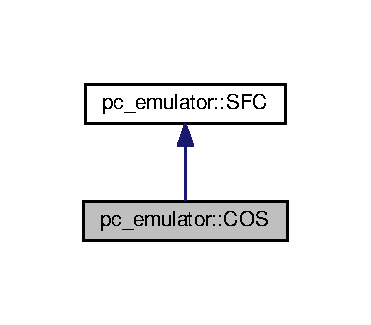
\includegraphics[width=178pt]{classpc__emulator_1_1COS__inherit__graph}
\end{center}
\end{figure}


Collaboration diagram for pc\+\_\+emulator\+:\+:C\+OS\+:
\nopagebreak
\begin{figure}[H]
\begin{center}
\leavevmode
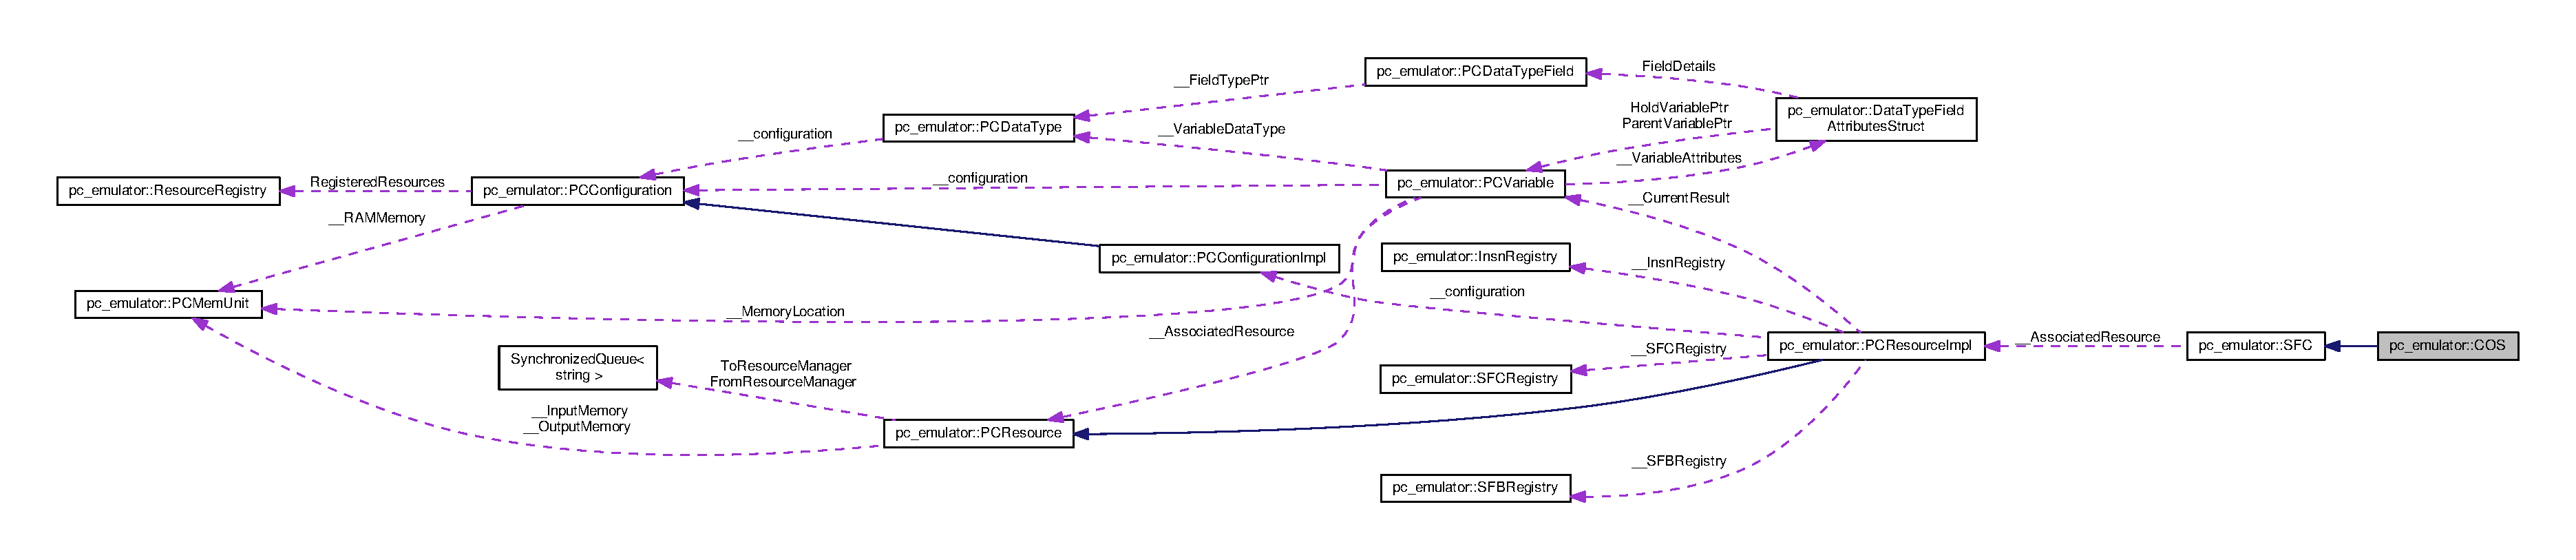
\includegraphics[width=350pt]{classpc__emulator_1_1COS__coll__graph}
\end{center}
\end{figure}
\subsection*{Public Member Functions}
\begin{DoxyCompactItemize}
\item 
{\bfseries C\+OS} (\hyperlink{classpc__emulator_1_1PCResourceImpl}{P\+C\+Resource\+Impl} $\ast$Associated\+Resource)\hypertarget{classpc__emulator_1_1COS_a2285617f9d1c039b4df01f709734dec5}{}\label{classpc__emulator_1_1COS_a2285617f9d1c039b4df01f709734dec5}

\item 
void \hyperlink{classpc__emulator_1_1COS_a66dc96f691d55d42fa20c55a5ed71a4f}{Execute} (\hyperlink{classpc__emulator_1_1PCVariable}{P\+C\+Variable} $\ast$Current\+Result, std\+::vector$<$ \hyperlink{classpc__emulator_1_1PCVariable}{P\+C\+Variable} $\ast$ $>$ \&Operands)
\begin{DoxyCompactList}\small\item\em Called to execute the sfc. \end{DoxyCompactList}\end{DoxyCompactItemize}
\subsection*{Additional Inherited Members}


\subsection{Detailed Description}
Definition of \hyperlink{classpc__emulator_1_1COS}{C\+OS} \hyperlink{classpc__emulator_1_1SFC}{S\+FC}. 

\subsection{Member Function Documentation}
\index{pc\+\_\+emulator\+::\+C\+OS@{pc\+\_\+emulator\+::\+C\+OS}!Execute@{Execute}}
\index{Execute@{Execute}!pc\+\_\+emulator\+::\+C\+OS@{pc\+\_\+emulator\+::\+C\+OS}}
\subsubsection[{\texorpdfstring{Execute(\+P\+C\+Variable $\ast$\+Current\+Result, std\+::vector$<$ P\+C\+Variable $\ast$ $>$ \&\+Operands)}{Execute(PCVariable *CurrentResult, std::vector< PCVariable * > &Operands)}}]{\setlength{\rightskip}{0pt plus 5cm}void pc\+\_\+emulator\+::\+C\+O\+S\+::\+Execute (
\begin{DoxyParamCaption}
\item[{{\bf P\+C\+Variable} $\ast$}]{Current\+Result, }
\item[{std\+::vector$<$ {\bf P\+C\+Variable} $\ast$ $>$ \&}]{Operands}
\end{DoxyParamCaption}
)\hspace{0.3cm}{\ttfamily [virtual]}}\hypertarget{classpc__emulator_1_1COS_a66dc96f691d55d42fa20c55a5ed71a4f}{}\label{classpc__emulator_1_1COS_a66dc96f691d55d42fa20c55a5ed71a4f}


Called to execute the sfc. 


\begin{DoxyParams}{Parameters}
{\em Current\+Result} & The Current\+Result register of the task executing this \hyperlink{classpc__emulator_1_1SFC}{S\+FC} \\
\hline
{\em Operands} & Operands to the sfc \\
\hline
\end{DoxyParams}


Implements \hyperlink{classpc__emulator_1_1SFC_ab206c80fc0e429c56672b4f6a0ca8635}{pc\+\_\+emulator\+::\+S\+FC}.



The documentation for this class was generated from the following file\+:\begin{DoxyCompactItemize}
\item 
src/pc\+\_\+emulator/include/sfc/cos.\+h\end{DoxyCompactItemize}

\hypertarget{structpc__emulator_1_1DataTypeFieldAttributesStruct}{}\section{pc\+\_\+emulator\+:\+:Data\+Type\+Field\+Attributes\+Struct Struct Reference}
\label{structpc__emulator_1_1DataTypeFieldAttributesStruct}\index{pc\+\_\+emulator\+::\+Data\+Type\+Field\+Attributes\+Struct@{pc\+\_\+emulator\+::\+Data\+Type\+Field\+Attributes\+Struct}}


Details of a data-\/type field.  




{\ttfamily \#include $<$pc\+\_\+variable.\+h$>$}



Collaboration diagram for pc\+\_\+emulator\+:\+:Data\+Type\+Field\+Attributes\+Struct\+:\nopagebreak
\begin{figure}[H]
\begin{center}
\leavevmode
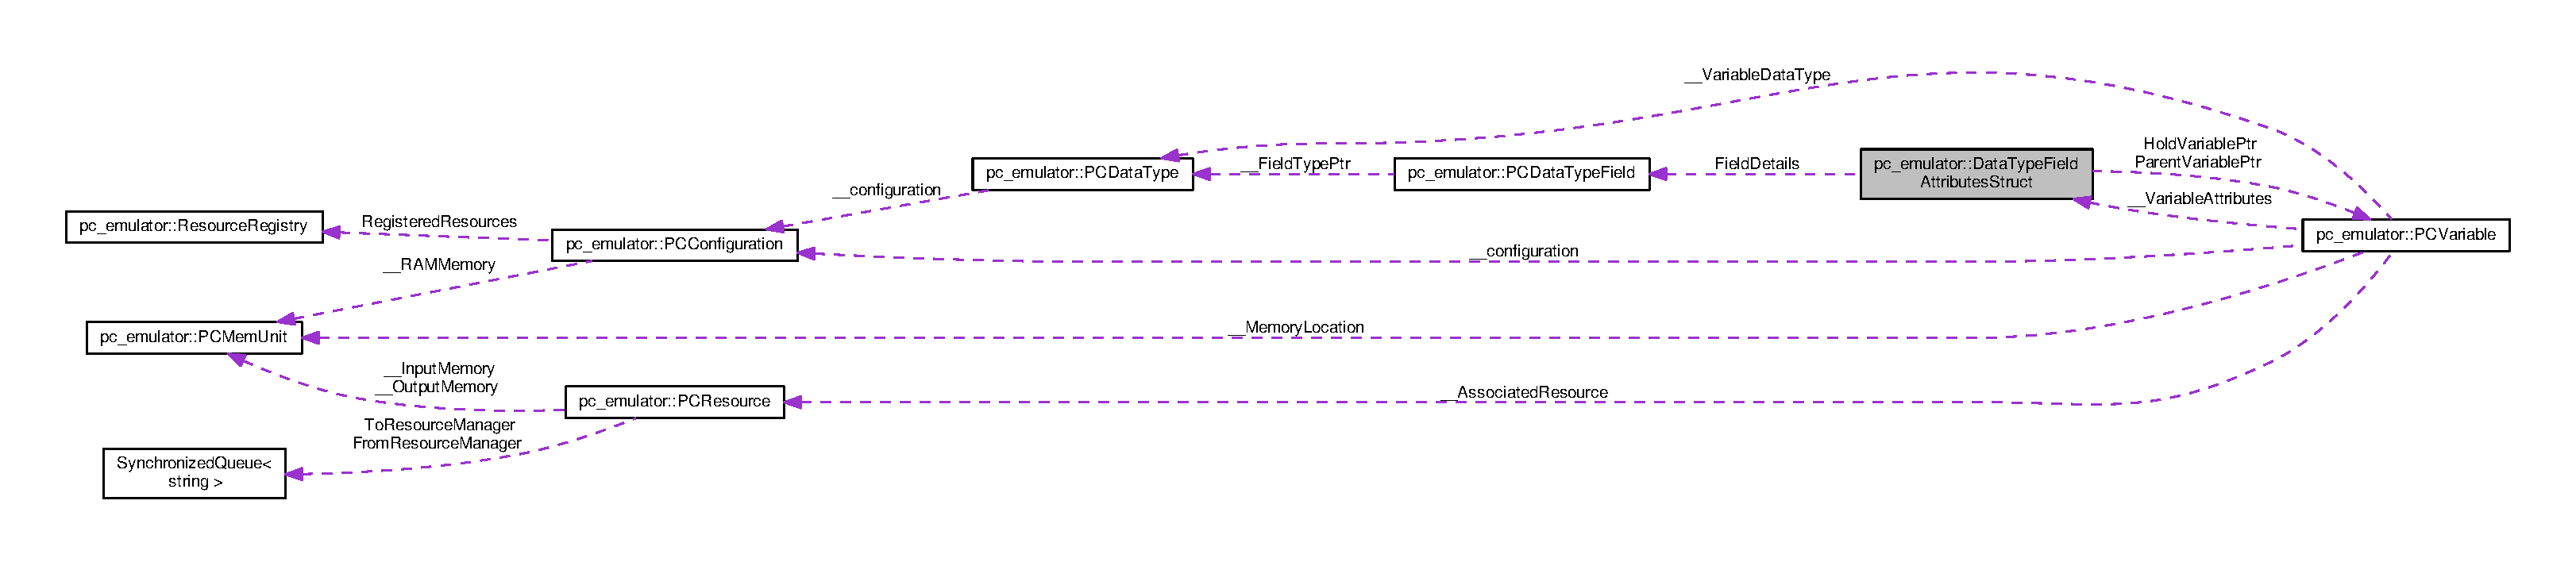
\includegraphics[width=350pt]{structpc__emulator_1_1DataTypeFieldAttributesStruct__coll__graph}
\end{center}
\end{figure}
\subsection*{Public Attributes}
\begin{DoxyCompactItemize}
\item 
string \hyperlink{structpc__emulator_1_1DataTypeFieldAttributesStruct_a38b068714c3b4e3bb59cb5406fbb93f2}{Nested\+Field\+Name}
\item 
unsigned long \hyperlink{structpc__emulator_1_1DataTypeFieldAttributesStruct_a9690def189b94d7515ae0ef00f3470ff}{Relative\+Offset}
\item 
\hyperlink{classpc__emulator_1_1PCDataTypeField}{P\+C\+Data\+Type\+Field} \hyperlink{structpc__emulator_1_1DataTypeFieldAttributesStruct_af464d3e0536e9a2a2e5ad6dfc0e91b1c}{Field\+Details}
\item 
\hyperlink{classpc__emulator_1_1PCVariable}{P\+C\+Variable} $\ast$ \hyperlink{structpc__emulator_1_1DataTypeFieldAttributesStruct_a704592013b2e84005a2f8c0a79e36efe}{Hold\+Variable\+Ptr}
\item 
\hyperlink{classpc__emulator_1_1PCVariable}{P\+C\+Variable} $\ast$ \hyperlink{structpc__emulator_1_1DataTypeFieldAttributesStruct_a8ef95a5a44edd724fc88884d969ee65e}{Parent\+Variable\+Ptr}
\end{DoxyCompactItemize}


\subsection{Detailed Description}
Details of a data-\/type field. 

\subsection{Member Data Documentation}
\index{pc\+\_\+emulator\+::\+Data\+Type\+Field\+Attributes\+Struct@{pc\+\_\+emulator\+::\+Data\+Type\+Field\+Attributes\+Struct}!Field\+Details@{Field\+Details}}
\index{Field\+Details@{Field\+Details}!pc\+\_\+emulator\+::\+Data\+Type\+Field\+Attributes\+Struct@{pc\+\_\+emulator\+::\+Data\+Type\+Field\+Attributes\+Struct}}
\subsubsection[{\texorpdfstring{Field\+Details}{FieldDetails}}]{\setlength{\rightskip}{0pt plus 5cm}{\bf P\+C\+Data\+Type\+Field} pc\+\_\+emulator\+::\+Data\+Type\+Field\+Attributes\+Struct\+::\+Field\+Details}\hypertarget{structpc__emulator_1_1DataTypeFieldAttributesStruct_af464d3e0536e9a2a2e5ad6dfc0e91b1c}{}\label{structpc__emulator_1_1DataTypeFieldAttributesStruct_af464d3e0536e9a2a2e5ad6dfc0e91b1c}
More details on the field \index{pc\+\_\+emulator\+::\+Data\+Type\+Field\+Attributes\+Struct@{pc\+\_\+emulator\+::\+Data\+Type\+Field\+Attributes\+Struct}!Hold\+Variable\+Ptr@{Hold\+Variable\+Ptr}}
\index{Hold\+Variable\+Ptr@{Hold\+Variable\+Ptr}!pc\+\_\+emulator\+::\+Data\+Type\+Field\+Attributes\+Struct@{pc\+\_\+emulator\+::\+Data\+Type\+Field\+Attributes\+Struct}}
\subsubsection[{\texorpdfstring{Hold\+Variable\+Ptr}{HoldVariablePtr}}]{\setlength{\rightskip}{0pt plus 5cm}{\bf P\+C\+Variable}$\ast$ pc\+\_\+emulator\+::\+Data\+Type\+Field\+Attributes\+Struct\+::\+Hold\+Variable\+Ptr}\hypertarget{structpc__emulator_1_1DataTypeFieldAttributesStruct_a704592013b2e84005a2f8c0a79e36efe}{}\label{structpc__emulator_1_1DataTypeFieldAttributesStruct_a704592013b2e84005a2f8c0a79e36efe}
This field is set to a value different from the Parent\+Variable\+Ptr iff the one or more of the intermediate nested fields are pointers. In that case it is set to the outermost pointer \index{pc\+\_\+emulator\+::\+Data\+Type\+Field\+Attributes\+Struct@{pc\+\_\+emulator\+::\+Data\+Type\+Field\+Attributes\+Struct}!Nested\+Field\+Name@{Nested\+Field\+Name}}
\index{Nested\+Field\+Name@{Nested\+Field\+Name}!pc\+\_\+emulator\+::\+Data\+Type\+Field\+Attributes\+Struct@{pc\+\_\+emulator\+::\+Data\+Type\+Field\+Attributes\+Struct}}
\subsubsection[{\texorpdfstring{Nested\+Field\+Name}{NestedFieldName}}]{\setlength{\rightskip}{0pt plus 5cm}string pc\+\_\+emulator\+::\+Data\+Type\+Field\+Attributes\+Struct\+::\+Nested\+Field\+Name}\hypertarget{structpc__emulator_1_1DataTypeFieldAttributesStruct_a38b068714c3b4e3bb59cb5406fbb93f2}{}\label{structpc__emulator_1_1DataTypeFieldAttributesStruct_a38b068714c3b4e3bb59cb5406fbb93f2}
Nested Field Name relative to the data type of Parent\+Variable\+Ptr \index{pc\+\_\+emulator\+::\+Data\+Type\+Field\+Attributes\+Struct@{pc\+\_\+emulator\+::\+Data\+Type\+Field\+Attributes\+Struct}!Parent\+Variable\+Ptr@{Parent\+Variable\+Ptr}}
\index{Parent\+Variable\+Ptr@{Parent\+Variable\+Ptr}!pc\+\_\+emulator\+::\+Data\+Type\+Field\+Attributes\+Struct@{pc\+\_\+emulator\+::\+Data\+Type\+Field\+Attributes\+Struct}}
\subsubsection[{\texorpdfstring{Parent\+Variable\+Ptr}{ParentVariablePtr}}]{\setlength{\rightskip}{0pt plus 5cm}{\bf P\+C\+Variable}$\ast$ pc\+\_\+emulator\+::\+Data\+Type\+Field\+Attributes\+Struct\+::\+Parent\+Variable\+Ptr}\hypertarget{structpc__emulator_1_1DataTypeFieldAttributesStruct_a8ef95a5a44edd724fc88884d969ee65e}{}\label{structpc__emulator_1_1DataTypeFieldAttributesStruct_a8ef95a5a44edd724fc88884d969ee65e}
This field is set to point to the variable which want\textquotesingle{}s to get attributes of the nested field \index{pc\+\_\+emulator\+::\+Data\+Type\+Field\+Attributes\+Struct@{pc\+\_\+emulator\+::\+Data\+Type\+Field\+Attributes\+Struct}!Relative\+Offset@{Relative\+Offset}}
\index{Relative\+Offset@{Relative\+Offset}!pc\+\_\+emulator\+::\+Data\+Type\+Field\+Attributes\+Struct@{pc\+\_\+emulator\+::\+Data\+Type\+Field\+Attributes\+Struct}}
\subsubsection[{\texorpdfstring{Relative\+Offset}{RelativeOffset}}]{\setlength{\rightskip}{0pt plus 5cm}unsigned long pc\+\_\+emulator\+::\+Data\+Type\+Field\+Attributes\+Struct\+::\+Relative\+Offset}\hypertarget{structpc__emulator_1_1DataTypeFieldAttributesStruct_a9690def189b94d7515ae0ef00f3470ff}{}\label{structpc__emulator_1_1DataTypeFieldAttributesStruct_a9690def189b94d7515ae0ef00f3470ff}
The data corresponding to the nested field is stored at the specified relative offset from the start of the Hold\+Variabl\+Ptr\textquotesingle{}s memory location 

The documentation for this struct was generated from the following file\+:\begin{DoxyCompactItemize}
\item 
src/pc\+\_\+emulator/include/pc\+\_\+variable.\+h\end{DoxyCompactItemize}

\hypertarget{classpc__emulator_1_1DataTypeRegistry}{}\section{pc\+\_\+emulator\+:\+:Data\+Type\+Registry Class Reference}
\label{classpc__emulator_1_1DataTypeRegistry}\index{pc\+\_\+emulator\+::\+Data\+Type\+Registry@{pc\+\_\+emulator\+::\+Data\+Type\+Registry}}


Registers and tracks data types.  




{\ttfamily \#include $<$pc\+\_\+datatype\+\_\+registry.\+h$>$}

\subsection*{Public Member Functions}
\begin{DoxyCompactItemize}
\item 
\hyperlink{classpc__emulator_1_1DataTypeRegistry_ae181a1e06e9c371b478f3f4a40aa3d05}{Data\+Type\+Registry} (\hyperlink{classpc__emulator_1_1PCConfiguration}{P\+C\+Configuration} $\ast$configuration)\hypertarget{classpc__emulator_1_1DataTypeRegistry_ae181a1e06e9c371b478f3f4a40aa3d05}{}\label{classpc__emulator_1_1DataTypeRegistry_ae181a1e06e9c371b478f3f4a40aa3d05}

\begin{DoxyCompactList}\small\item\em Constructor. \end{DoxyCompactList}\item 
void \hyperlink{classpc__emulator_1_1DataTypeRegistry_aeb42f0888bb6a866c5cb497f4c55e79d}{Register\+Data\+Type} (string Data\+Type\+Name, std\+::unique\+\_\+ptr$<$ \hyperlink{classpc__emulator_1_1PCDataType}{P\+C\+Data\+Type} $>$ Data\+Type)\hypertarget{classpc__emulator_1_1DataTypeRegistry_aeb42f0888bb6a866c5cb497f4c55e79d}{}\label{classpc__emulator_1_1DataTypeRegistry_aeb42f0888bb6a866c5cb497f4c55e79d}

\begin{DoxyCompactList}\small\item\em Register new data type. \end{DoxyCompactList}\item 
\hyperlink{classpc__emulator_1_1PCDataType}{P\+C\+Data\+Type} $\ast$ \hyperlink{classpc__emulator_1_1DataTypeRegistry_a1140ec01678f40daed5035f5e8cac6ce}{Get\+Data\+Type} (string Data\+Type\+Name)\hypertarget{classpc__emulator_1_1DataTypeRegistry_a1140ec01678f40daed5035f5e8cac6ce}{}\label{classpc__emulator_1_1DataTypeRegistry_a1140ec01678f40daed5035f5e8cac6ce}

\begin{DoxyCompactList}\small\item\em Retrieves data type with the specified name. \end{DoxyCompactList}\item 
void \hyperlink{classpc__emulator_1_1DataTypeRegistry_ae67e87cb84212168f8784fe90d95a3dc}{Cleanup} ()\hypertarget{classpc__emulator_1_1DataTypeRegistry_ae67e87cb84212168f8784fe90d95a3dc}{}\label{classpc__emulator_1_1DataTypeRegistry_ae67e87cb84212168f8784fe90d95a3dc}

\begin{DoxyCompactList}\small\item\em Clean\textquotesingle{}s up all registered data types. \end{DoxyCompactList}\end{DoxyCompactItemize}


\subsection{Detailed Description}
Registers and tracks data types. 

The documentation for this class was generated from the following file\+:\begin{DoxyCompactItemize}
\item 
src/pc\+\_\+emulator/include/pc\+\_\+datatype\+\_\+registry.\+h\end{DoxyCompactItemize}

\hypertarget{classpc__emulator_1_1DataTypeUtils}{}\section{pc\+\_\+emulator\+:\+:Data\+Type\+Utils Class Reference}
\label{classpc__emulator_1_1DataTypeUtils}\index{pc\+\_\+emulator\+::\+Data\+Type\+Utils@{pc\+\_\+emulator\+::\+Data\+Type\+Utils}}


Util class for converting passed strings to elementary data types.  




{\ttfamily \#include $<$pc\+\_\+datatype.\+h$>$}

\subsection*{Static Public Member Functions}
\begin{DoxyCompactItemize}
\item 
static bool \hyperlink{classpc__emulator_1_1DataTypeUtils_a299a4f130ef9cd9529c9e2db79669f80}{Value\+To\+Bool} (string Value, bool \&Bool\+Value)\hypertarget{classpc__emulator_1_1DataTypeUtils_a299a4f130ef9cd9529c9e2db79669f80}{}\label{classpc__emulator_1_1DataTypeUtils_a299a4f130ef9cd9529c9e2db79669f80}

\begin{DoxyCompactList}\small\item\em Convert passed value to bool. Return True on success. \end{DoxyCompactList}\item 
static bool \hyperlink{classpc__emulator_1_1DataTypeUtils_a7f842d480fed9a96e3e3971565d1193e}{Value\+To\+Byte} (string Value, uint8\+\_\+t \&Byte\+Value)\hypertarget{classpc__emulator_1_1DataTypeUtils_a7f842d480fed9a96e3e3971565d1193e}{}\label{classpc__emulator_1_1DataTypeUtils_a7f842d480fed9a96e3e3971565d1193e}

\begin{DoxyCompactList}\small\item\em Convert passed value to byte. Return True on success. \end{DoxyCompactList}\item 
static bool \hyperlink{classpc__emulator_1_1DataTypeUtils_a150c8f2968f3d419708da44ffdada4b1}{Value\+To\+Word} (string Value, uint16\+\_\+t \&Word\+Value)\hypertarget{classpc__emulator_1_1DataTypeUtils_a150c8f2968f3d419708da44ffdada4b1}{}\label{classpc__emulator_1_1DataTypeUtils_a150c8f2968f3d419708da44ffdada4b1}

\begin{DoxyCompactList}\small\item\em Convert passed value to word. Return True on success. \end{DoxyCompactList}\item 
static bool \hyperlink{classpc__emulator_1_1DataTypeUtils_a5d51cb72a80928caa8f1b2c1f6dec580}{Value\+To\+D\+Word} (string Value, uint32\+\_\+t \&D\+Word\+Value)\hypertarget{classpc__emulator_1_1DataTypeUtils_a5d51cb72a80928caa8f1b2c1f6dec580}{}\label{classpc__emulator_1_1DataTypeUtils_a5d51cb72a80928caa8f1b2c1f6dec580}

\begin{DoxyCompactList}\small\item\em Convert passed value to dword. Return True on success. \end{DoxyCompactList}\item 
static bool \hyperlink{classpc__emulator_1_1DataTypeUtils_a1830130ad79852bcbbe2b20bd30bb21b}{Value\+To\+L\+Word} (string Value, uint64\+\_\+t \&L\+Word\+Value)\hypertarget{classpc__emulator_1_1DataTypeUtils_a1830130ad79852bcbbe2b20bd30bb21b}{}\label{classpc__emulator_1_1DataTypeUtils_a1830130ad79852bcbbe2b20bd30bb21b}

\begin{DoxyCompactList}\small\item\em Convert passed value to lword. Return True on success. \end{DoxyCompactList}\item 
static bool \hyperlink{classpc__emulator_1_1DataTypeUtils_a8a43a772fca227b96240a38022c5ceb9}{Value\+To\+Char} (string Value, char \&Char\+Value)\hypertarget{classpc__emulator_1_1DataTypeUtils_a8a43a772fca227b96240a38022c5ceb9}{}\label{classpc__emulator_1_1DataTypeUtils_a8a43a772fca227b96240a38022c5ceb9}

\begin{DoxyCompactList}\small\item\em Convert passed value to char. Return True on success. \end{DoxyCompactList}\item 
static bool \hyperlink{classpc__emulator_1_1DataTypeUtils_a7a87e26bc6fd076f012f0ba02c96c866}{Value\+To\+Int} (string Value, int16\+\_\+t \&Int\+Value)\hypertarget{classpc__emulator_1_1DataTypeUtils_a7a87e26bc6fd076f012f0ba02c96c866}{}\label{classpc__emulator_1_1DataTypeUtils_a7a87e26bc6fd076f012f0ba02c96c866}

\begin{DoxyCompactList}\small\item\em Convert passed value to int. Return True on success. \end{DoxyCompactList}\item 
static bool \hyperlink{classpc__emulator_1_1DataTypeUtils_a6250d59717b5dff66f0847a9ecf09709}{Value\+To\+Sint} (string Value, int8\+\_\+t \&Sint\+Value)\hypertarget{classpc__emulator_1_1DataTypeUtils_a6250d59717b5dff66f0847a9ecf09709}{}\label{classpc__emulator_1_1DataTypeUtils_a6250d59717b5dff66f0847a9ecf09709}

\begin{DoxyCompactList}\small\item\em Convert passed value to sint. Return True on success. \end{DoxyCompactList}\item 
static bool \hyperlink{classpc__emulator_1_1DataTypeUtils_a42b5e4153755796a740a2450b404a818}{Value\+To\+Dint} (string Value, int32\+\_\+t \&Dint\+Value)\hypertarget{classpc__emulator_1_1DataTypeUtils_a42b5e4153755796a740a2450b404a818}{}\label{classpc__emulator_1_1DataTypeUtils_a42b5e4153755796a740a2450b404a818}

\begin{DoxyCompactList}\small\item\em Convert passed value to dint. Return True on success. \end{DoxyCompactList}\item 
static bool \hyperlink{classpc__emulator_1_1DataTypeUtils_abcb1021b4660fc9c65b5fc0f81f43154}{Value\+To\+Lint} (string Value, int64\+\_\+t \&Lint\+Value)\hypertarget{classpc__emulator_1_1DataTypeUtils_abcb1021b4660fc9c65b5fc0f81f43154}{}\label{classpc__emulator_1_1DataTypeUtils_abcb1021b4660fc9c65b5fc0f81f43154}

\begin{DoxyCompactList}\small\item\em Convert passed value to lint. Return True on success. \end{DoxyCompactList}\item 
static bool \hyperlink{classpc__emulator_1_1DataTypeUtils_a1a3703bbf73bfb70e85f93d3a248935a}{Value\+To\+Uint} (string Value, uint16\+\_\+t \&Uint\+Value)\hypertarget{classpc__emulator_1_1DataTypeUtils_a1a3703bbf73bfb70e85f93d3a248935a}{}\label{classpc__emulator_1_1DataTypeUtils_a1a3703bbf73bfb70e85f93d3a248935a}

\begin{DoxyCompactList}\small\item\em Convert passed value to uint. Return True on success. \end{DoxyCompactList}\item 
static bool \hyperlink{classpc__emulator_1_1DataTypeUtils_a9d027e2add6a18b3868a6ba0e57144e8}{Value\+To\+Usint} (string Value, uint8\+\_\+t \&Usint\+Value)\hypertarget{classpc__emulator_1_1DataTypeUtils_a9d027e2add6a18b3868a6ba0e57144e8}{}\label{classpc__emulator_1_1DataTypeUtils_a9d027e2add6a18b3868a6ba0e57144e8}

\begin{DoxyCompactList}\small\item\em Convert passed value to usint. Return True on success. \end{DoxyCompactList}\item 
static bool \hyperlink{classpc__emulator_1_1DataTypeUtils_ad27a5f01c5ccd778bdcc8df9db37fb92}{Value\+To\+Udint} (string Value, uint32\+\_\+t \&Udint\+Value)\hypertarget{classpc__emulator_1_1DataTypeUtils_ad27a5f01c5ccd778bdcc8df9db37fb92}{}\label{classpc__emulator_1_1DataTypeUtils_ad27a5f01c5ccd778bdcc8df9db37fb92}

\begin{DoxyCompactList}\small\item\em Convert passed value to udint. Return True on success. \end{DoxyCompactList}\item 
static bool \hyperlink{classpc__emulator_1_1DataTypeUtils_a7b492f75dc7c8ef0d82466ac6fc14735}{Value\+To\+Ulint} (string Value, uint64\+\_\+t \&Ulint\+Value)\hypertarget{classpc__emulator_1_1DataTypeUtils_a7b492f75dc7c8ef0d82466ac6fc14735}{}\label{classpc__emulator_1_1DataTypeUtils_a7b492f75dc7c8ef0d82466ac6fc14735}

\begin{DoxyCompactList}\small\item\em Convert passed value to ulint. Return True on success. \end{DoxyCompactList}\item 
static bool \hyperlink{classpc__emulator_1_1DataTypeUtils_a44cf3e9125dbe71a5de57d5a7f06a5df}{Value\+To\+Real} (string Value, float \&Real\+Value)\hypertarget{classpc__emulator_1_1DataTypeUtils_a44cf3e9125dbe71a5de57d5a7f06a5df}{}\label{classpc__emulator_1_1DataTypeUtils_a44cf3e9125dbe71a5de57d5a7f06a5df}

\begin{DoxyCompactList}\small\item\em Convert passed value to real. Return True on success. \end{DoxyCompactList}\item 
static bool \hyperlink{classpc__emulator_1_1DataTypeUtils_ade1a844fd50a9001d71ff1e295019132}{Value\+To\+L\+Real} (string Value, double \&L\+Real\+Value)\hypertarget{classpc__emulator_1_1DataTypeUtils_ade1a844fd50a9001d71ff1e295019132}{}\label{classpc__emulator_1_1DataTypeUtils_ade1a844fd50a9001d71ff1e295019132}

\begin{DoxyCompactList}\small\item\em Convert passed value to lreal. Return True on success. \end{DoxyCompactList}\item 
static bool \hyperlink{classpc__emulator_1_1DataTypeUtils_a7bdb5617cf8054717f07b75b13735c52}{Value\+To\+Time} (string Value, \hyperlink{structpc__emulator_1_1TIMEDataType}{Time\+Type} \&Time)\hypertarget{classpc__emulator_1_1DataTypeUtils_a7bdb5617cf8054717f07b75b13735c52}{}\label{classpc__emulator_1_1DataTypeUtils_a7bdb5617cf8054717f07b75b13735c52}

\begin{DoxyCompactList}\small\item\em Convert passed value to time. Return True on success. \end{DoxyCompactList}\item 
static bool \hyperlink{classpc__emulator_1_1DataTypeUtils_abbce892d1d360df0839af7619a08498b}{Value\+To\+T\+OD} (string Value, \hyperlink{structpc__emulator_1_1TODDataType}{T\+O\+D\+Type} \&T\+OD)\hypertarget{classpc__emulator_1_1DataTypeUtils_abbce892d1d360df0839af7619a08498b}{}\label{classpc__emulator_1_1DataTypeUtils_abbce892d1d360df0839af7619a08498b}

\begin{DoxyCompactList}\small\item\em Convert passed value to time of day. Return True on success. \end{DoxyCompactList}\item 
static bool \hyperlink{classpc__emulator_1_1DataTypeUtils_a4c2c00be81221d68ad0378a2c1d5f4e1}{Value\+To\+DT} (string Value, \hyperlink{structpc__emulator_1_1DateTODDataType}{Date\+T\+O\+D\+Data\+Type} \&Dt)\hypertarget{classpc__emulator_1_1DataTypeUtils_a4c2c00be81221d68ad0378a2c1d5f4e1}{}\label{classpc__emulator_1_1DataTypeUtils_a4c2c00be81221d68ad0378a2c1d5f4e1}

\begin{DoxyCompactList}\small\item\em Convert passed value to date and time. Return True on success. \end{DoxyCompactList}\item 
static bool \hyperlink{classpc__emulator_1_1DataTypeUtils_ad9dabf2772efc07427b69ac733dc3f33}{Value\+To\+Date} (string Value, \hyperlink{structpc__emulator_1_1DateDataType}{Date\+Type} \&Date)\hypertarget{classpc__emulator_1_1DataTypeUtils_ad9dabf2772efc07427b69ac733dc3f33}{}\label{classpc__emulator_1_1DataTypeUtils_ad9dabf2772efc07427b69ac733dc3f33}

\begin{DoxyCompactList}\small\item\em Convert passed value to date. Return True on success. \end{DoxyCompactList}\item 
static bool \hyperlink{classpc__emulator_1_1DataTypeUtils_a6b442f726a053b8f3e2982744ce1b939}{Bool\+To\+Any} (bool Value, int Data\+Type\+Category, string \&Result)\hypertarget{classpc__emulator_1_1DataTypeUtils_a6b442f726a053b8f3e2982744ce1b939}{}\label{classpc__emulator_1_1DataTypeUtils_a6b442f726a053b8f3e2982744ce1b939}

\begin{DoxyCompactList}\small\item\em Convert passed bool Value to a equivalent string description of specified data type category. \end{DoxyCompactList}\item 
static bool \hyperlink{classpc__emulator_1_1DataTypeUtils_a53d055de7df09456a91f70803040997f}{Byte\+To\+Any} (uint8\+\_\+t Value, int Data\+Type\+Category, string \&Result)\hypertarget{classpc__emulator_1_1DataTypeUtils_a53d055de7df09456a91f70803040997f}{}\label{classpc__emulator_1_1DataTypeUtils_a53d055de7df09456a91f70803040997f}

\begin{DoxyCompactList}\small\item\em Convert passed byte Value to a equivalent string description of specified data type category. \end{DoxyCompactList}\item 
static bool \hyperlink{classpc__emulator_1_1DataTypeUtils_acab946275296df9246950cff4bfac8d4}{Word\+To\+Any} (uint16\+\_\+t Value, int Data\+Type\+Category, string \&Result)\hypertarget{classpc__emulator_1_1DataTypeUtils_acab946275296df9246950cff4bfac8d4}{}\label{classpc__emulator_1_1DataTypeUtils_acab946275296df9246950cff4bfac8d4}

\begin{DoxyCompactList}\small\item\em Convert passed word Value to a equivalent string description of specified data type category. \end{DoxyCompactList}\item 
static bool \hyperlink{classpc__emulator_1_1DataTypeUtils_a3d2aebc4144750c83233a935494bbd0b}{D\+Word\+To\+Any} (uint32\+\_\+t Value, int Data\+Type\+Category, string \&Result)\hypertarget{classpc__emulator_1_1DataTypeUtils_a3d2aebc4144750c83233a935494bbd0b}{}\label{classpc__emulator_1_1DataTypeUtils_a3d2aebc4144750c83233a935494bbd0b}

\begin{DoxyCompactList}\small\item\em Convert passed dword Value to a equivalent string description of specified data type category. \end{DoxyCompactList}\item 
static bool \hyperlink{classpc__emulator_1_1DataTypeUtils_aaa48015d360664699a240cd900055977}{L\+Word\+To\+Any} (uint64\+\_\+t Value, int Data\+Type\+Category, string \&Result)\hypertarget{classpc__emulator_1_1DataTypeUtils_aaa48015d360664699a240cd900055977}{}\label{classpc__emulator_1_1DataTypeUtils_aaa48015d360664699a240cd900055977}

\begin{DoxyCompactList}\small\item\em Convert passed lword Value to a equivalent string description of specified data type category. \end{DoxyCompactList}\item 
static bool \hyperlink{classpc__emulator_1_1DataTypeUtils_abe6ad0fa1288a76c81afc1942a6af75c}{Char\+To\+Any} (char Value, int Data\+Type\+Category, string \&Result)\hypertarget{classpc__emulator_1_1DataTypeUtils_abe6ad0fa1288a76c81afc1942a6af75c}{}\label{classpc__emulator_1_1DataTypeUtils_abe6ad0fa1288a76c81afc1942a6af75c}

\begin{DoxyCompactList}\small\item\em Convert passed char Value to a equivalent string description of specified data type category. \end{DoxyCompactList}\item 
static bool \hyperlink{classpc__emulator_1_1DataTypeUtils_a670972c6d0ff39ed1847f5faf9c70ee6}{Int\+To\+Any} (int16\+\_\+t Value, int Data\+Type\+Category, string \&Result)\hypertarget{classpc__emulator_1_1DataTypeUtils_a670972c6d0ff39ed1847f5faf9c70ee6}{}\label{classpc__emulator_1_1DataTypeUtils_a670972c6d0ff39ed1847f5faf9c70ee6}

\begin{DoxyCompactList}\small\item\em Convert passed int Value to a equivalent string description of specified data type category. \end{DoxyCompactList}\item 
static bool \hyperlink{classpc__emulator_1_1DataTypeUtils_a060e4406c657e256fb52994c8df26e2a}{S\+Int\+To\+Any} (int8\+\_\+t Value, int Data\+Type\+Category, string \&Result)\hypertarget{classpc__emulator_1_1DataTypeUtils_a060e4406c657e256fb52994c8df26e2a}{}\label{classpc__emulator_1_1DataTypeUtils_a060e4406c657e256fb52994c8df26e2a}

\begin{DoxyCompactList}\small\item\em Convert passed sint Value to a equivalent string description of specified data type category. \end{DoxyCompactList}\item 
static bool \hyperlink{classpc__emulator_1_1DataTypeUtils_a02738761f3d14d3e8cd4a6f5da03faee}{D\+Int\+To\+Any} (int32\+\_\+t Value, int Data\+Type\+Category, string \&Result)\hypertarget{classpc__emulator_1_1DataTypeUtils_a02738761f3d14d3e8cd4a6f5da03faee}{}\label{classpc__emulator_1_1DataTypeUtils_a02738761f3d14d3e8cd4a6f5da03faee}

\begin{DoxyCompactList}\small\item\em Convert passed dint Value to a equivalent string description of specified data type category. \end{DoxyCompactList}\item 
static bool \hyperlink{classpc__emulator_1_1DataTypeUtils_aa28b3185bb419706594f4b9b660fe932}{L\+Int\+To\+Any} (int64\+\_\+t Value, int Data\+Type\+Category, string \&Result)\hypertarget{classpc__emulator_1_1DataTypeUtils_aa28b3185bb419706594f4b9b660fe932}{}\label{classpc__emulator_1_1DataTypeUtils_aa28b3185bb419706594f4b9b660fe932}

\begin{DoxyCompactList}\small\item\em Convert passed lint Value to a equivalent string description of specified data type category. \end{DoxyCompactList}\item 
static bool \hyperlink{classpc__emulator_1_1DataTypeUtils_a2ac017f0098d96cecfadd6ef7b6b4c25}{U\+Int\+To\+Any} (uint16\+\_\+t Value, int Data\+Type\+Category, string \&Result)\hypertarget{classpc__emulator_1_1DataTypeUtils_a2ac017f0098d96cecfadd6ef7b6b4c25}{}\label{classpc__emulator_1_1DataTypeUtils_a2ac017f0098d96cecfadd6ef7b6b4c25}

\begin{DoxyCompactList}\small\item\em Convert passed uint Value to a equivalent string description of specified data type category. \end{DoxyCompactList}\item 
static bool \hyperlink{classpc__emulator_1_1DataTypeUtils_a045630f4aa8a7fb18d08092321a8af8f}{U\+Sint\+To\+Any} (uint8\+\_\+t Value, int Data\+Type\+Category, string \&Result)\hypertarget{classpc__emulator_1_1DataTypeUtils_a045630f4aa8a7fb18d08092321a8af8f}{}\label{classpc__emulator_1_1DataTypeUtils_a045630f4aa8a7fb18d08092321a8af8f}

\begin{DoxyCompactList}\small\item\em Convert passed usint Value to a equivalent string description of specified data type category. \end{DoxyCompactList}\item 
static bool \hyperlink{classpc__emulator_1_1DataTypeUtils_aa33fffc63ceb8433d12ccd4880f2f56c}{U\+Dint\+To\+Any} (uint32\+\_\+t Value, int Data\+Type\+Category, string \&Result)\hypertarget{classpc__emulator_1_1DataTypeUtils_aa33fffc63ceb8433d12ccd4880f2f56c}{}\label{classpc__emulator_1_1DataTypeUtils_aa33fffc63ceb8433d12ccd4880f2f56c}

\begin{DoxyCompactList}\small\item\em Convert passed udint Value to a equivalent string description of specified data type category. \end{DoxyCompactList}\item 
static bool \hyperlink{classpc__emulator_1_1DataTypeUtils_a1c58bda1f1704afe30da939e02791f56}{Ulint\+To\+Any} (uint64\+\_\+t Value, int Data\+Type\+Category, string \&Result)\hypertarget{classpc__emulator_1_1DataTypeUtils_a1c58bda1f1704afe30da939e02791f56}{}\label{classpc__emulator_1_1DataTypeUtils_a1c58bda1f1704afe30da939e02791f56}

\begin{DoxyCompactList}\small\item\em Convert passed ulint Value to a equivalent string description of specified data type category. \end{DoxyCompactList}\item 
static bool \hyperlink{classpc__emulator_1_1DataTypeUtils_ad67f9a13f0eb789577b9f3c5561c4e55}{Real\+To\+Any} (float Value, int Data\+Type\+Category, string \&Result)\hypertarget{classpc__emulator_1_1DataTypeUtils_ad67f9a13f0eb789577b9f3c5561c4e55}{}\label{classpc__emulator_1_1DataTypeUtils_ad67f9a13f0eb789577b9f3c5561c4e55}

\begin{DoxyCompactList}\small\item\em Convert passed real Value to a equivalent string description of specified data type category. \end{DoxyCompactList}\item 
static bool \hyperlink{classpc__emulator_1_1DataTypeUtils_a493525ae488d0d825858ea20701fd412}{L\+Real\+To\+Any} (double Value, int Data\+Type\+Category, string \&Result)\hypertarget{classpc__emulator_1_1DataTypeUtils_a493525ae488d0d825858ea20701fd412}{}\label{classpc__emulator_1_1DataTypeUtils_a493525ae488d0d825858ea20701fd412}

\begin{DoxyCompactList}\small\item\em Convert passed lreal Value to a equivalent string description of specified data type category. \end{DoxyCompactList}\item 
static string \hyperlink{classpc__emulator_1_1DataTypeUtils_ad9bd193c25786aea50df4b47dbd3b663}{D\+T\+To\+D\+T\+String} (\hyperlink{structpc__emulator_1_1DateTODDataType}{Date\+T\+O\+D\+Data\+Type} \&dt)\hypertarget{classpc__emulator_1_1DataTypeUtils_ad9bd193c25786aea50df4b47dbd3b663}{}\label{classpc__emulator_1_1DataTypeUtils_ad9bd193c25786aea50df4b47dbd3b663}

\begin{DoxyCompactList}\small\item\em Converts a Date\+Time object into a DT string. \end{DoxyCompactList}\item 
static string \hyperlink{classpc__emulator_1_1DataTypeUtils_a5ed4cdd86bd90996706c8c89f965f43b}{Date\+To\+D\+T\+String} (\hyperlink{structpc__emulator_1_1DateDataType}{Date\+Data\+Type} \&date1)\hypertarget{classpc__emulator_1_1DataTypeUtils_a5ed4cdd86bd90996706c8c89f965f43b}{}\label{classpc__emulator_1_1DataTypeUtils_a5ed4cdd86bd90996706c8c89f965f43b}

\begin{DoxyCompactList}\small\item\em Converts a Date object into a DT string. \end{DoxyCompactList}\item 
static void \hyperlink{classpc__emulator_1_1DataTypeUtils_a39040271d3313ca64ffd484cb76235e8}{Add\+To\+DT} (\hyperlink{structpc__emulator_1_1DateTODDataType}{Date\+T\+O\+D\+Data\+Type} \&Dt, \hyperlink{structpc__emulator_1_1TIMEDataType}{Time\+Type} \&Time)\hypertarget{classpc__emulator_1_1DataTypeUtils_a39040271d3313ca64ffd484cb76235e8}{}\label{classpc__emulator_1_1DataTypeUtils_a39040271d3313ca64ffd484cb76235e8}

\begin{DoxyCompactList}\small\item\em Adds time with a date time object. \end{DoxyCompactList}\item 
static void \hyperlink{classpc__emulator_1_1DataTypeUtils_a54cfe9dd10b69662ad68ff4f0844f619}{Add\+To\+T\+OD} (\hyperlink{structpc__emulator_1_1TODDataType}{T\+O\+D\+Data\+Type} \&tod, \hyperlink{structpc__emulator_1_1TIMEDataType}{Time\+Type} \&Time)\hypertarget{classpc__emulator_1_1DataTypeUtils_a54cfe9dd10b69662ad68ff4f0844f619}{}\label{classpc__emulator_1_1DataTypeUtils_a54cfe9dd10b69662ad68ff4f0844f619}

\begin{DoxyCompactList}\small\item\em Adds time with a time of day object. \end{DoxyCompactList}\item 
static void \hyperlink{classpc__emulator_1_1DataTypeUtils_a0086a7eba79bb1d0049d74e172103168}{Sub\+From\+DT} (\hyperlink{structpc__emulator_1_1DateTODDataType}{Date\+T\+O\+D\+Data\+Type} \&Dt, \hyperlink{structpc__emulator_1_1TIMEDataType}{Time\+Type} \&Time)\hypertarget{classpc__emulator_1_1DataTypeUtils_a0086a7eba79bb1d0049d74e172103168}{}\label{classpc__emulator_1_1DataTypeUtils_a0086a7eba79bb1d0049d74e172103168}

\begin{DoxyCompactList}\small\item\em Subtracts time from a date time object. \end{DoxyCompactList}\item 
static void \hyperlink{classpc__emulator_1_1DataTypeUtils_ae9646c27c41585a808f847c649043f24}{Sub\+From\+T\+OD} (\hyperlink{structpc__emulator_1_1TODDataType}{T\+O\+D\+Data\+Type} \&tod, \hyperlink{structpc__emulator_1_1TIMEDataType}{Time\+Type} \&Time)\hypertarget{classpc__emulator_1_1DataTypeUtils_ae9646c27c41585a808f847c649043f24}{}\label{classpc__emulator_1_1DataTypeUtils_ae9646c27c41585a808f847c649043f24}

\begin{DoxyCompactList}\small\item\em Subtracts time from a time of day object. \end{DoxyCompactList}\item 
static \hyperlink{structpc__emulator_1_1TIMEDataType}{Time\+Type} \hyperlink{classpc__emulator_1_1DataTypeUtils_a211df36821d3c8c3403481b4f164736d}{Sub\+D\+Ts} (\hyperlink{structpc__emulator_1_1DateTODDataType}{Date\+T\+O\+D\+Data\+Type} \&Dt1, \hyperlink{structpc__emulator_1_1DateTODDataType}{Date\+T\+O\+D\+Data\+Type} \&Dt2)\hypertarget{classpc__emulator_1_1DataTypeUtils_a211df36821d3c8c3403481b4f164736d}{}\label{classpc__emulator_1_1DataTypeUtils_a211df36821d3c8c3403481b4f164736d}

\begin{DoxyCompactList}\small\item\em Subtracts two date time objects and returns a time object. \end{DoxyCompactList}\item 
static \hyperlink{structpc__emulator_1_1TIMEDataType}{Time\+Type} \hyperlink{classpc__emulator_1_1DataTypeUtils_a4b694002d5039a511080fa55bea7fd87}{Sub\+T\+O\+Ds} (\hyperlink{structpc__emulator_1_1TODDataType}{T\+O\+D\+Data\+Type} \&tod1, \hyperlink{structpc__emulator_1_1TODDataType}{T\+O\+D\+Data\+Type} \&tod2)\hypertarget{classpc__emulator_1_1DataTypeUtils_a4b694002d5039a511080fa55bea7fd87}{}\label{classpc__emulator_1_1DataTypeUtils_a4b694002d5039a511080fa55bea7fd87}

\begin{DoxyCompactList}\small\item\em Subtracts two time of day objects and returns a time object. \end{DoxyCompactList}\item 
static \hyperlink{structpc__emulator_1_1TIMEDataType}{Time\+Type} \hyperlink{classpc__emulator_1_1DataTypeUtils_ada16478ce0110396b13a04a6edc0bfae}{Sub\+D\+A\+T\+Es} (\hyperlink{structpc__emulator_1_1DateDataType}{Date\+Data\+Type} \&date1, \hyperlink{structpc__emulator_1_1DateDataType}{Date\+Data\+Type} \&date2)\hypertarget{classpc__emulator_1_1DataTypeUtils_ada16478ce0110396b13a04a6edc0bfae}{}\label{classpc__emulator_1_1DataTypeUtils_ada16478ce0110396b13a04a6edc0bfae}

\begin{DoxyCompactList}\small\item\em Subtracts two date objects and returns a time object. \end{DoxyCompactList}\end{DoxyCompactItemize}


\subsection{Detailed Description}
Util class for converting passed strings to elementary data types. 

The documentation for this class was generated from the following file\+:\begin{DoxyCompactItemize}
\item 
src/pc\+\_\+emulator/include/pc\+\_\+datatype.\+h\end{DoxyCompactItemize}

\hypertarget{structpc__emulator_1_1DateDataType}{}\section{pc\+\_\+emulator\+:\+:Date\+Data\+Type Struct Reference}
\label{structpc__emulator_1_1DateDataType}\index{pc\+\_\+emulator\+::\+Date\+Data\+Type@{pc\+\_\+emulator\+::\+Date\+Data\+Type}}


The elementary Date data type containing year, month, day.  




{\ttfamily \#include $<$elementary\+\_\+datatypes.\+h$>$}

\subsection*{Public Member Functions}
\begin{DoxyCompactItemize}
\item 
\hyperlink{structpc__emulator_1_1DateDataType}{Date\+Data\+Type} \& \hyperlink{structpc__emulator_1_1DateDataType_a42c4dfced912cbcecd8dfd8848ee01e0}{operator+} (const \hyperlink{structpc__emulator_1_1DateDataType}{Date\+Data\+Type} \&a)\hypertarget{structpc__emulator_1_1DateDataType_a42c4dfced912cbcecd8dfd8848ee01e0}{}\label{structpc__emulator_1_1DateDataType_a42c4dfced912cbcecd8dfd8848ee01e0}

\begin{DoxyCompactList}\small\item\em Add operator for two date data types. Does nothing. \end{DoxyCompactList}\item 
\hyperlink{structpc__emulator_1_1DateDataType}{Date\+Data\+Type} \& \hyperlink{structpc__emulator_1_1DateDataType_ab2e6786ea12412121174a04639b06c00}{operator-\/} (const \hyperlink{structpc__emulator_1_1DateDataType}{Date\+Data\+Type} \&a)\hypertarget{structpc__emulator_1_1DateDataType_ab2e6786ea12412121174a04639b06c00}{}\label{structpc__emulator_1_1DateDataType_ab2e6786ea12412121174a04639b06c00}

\begin{DoxyCompactList}\small\item\em Sub operator for two date data types. Does nothing. \end{DoxyCompactList}\item 
\hyperlink{structpc__emulator_1_1DateDataType}{Date\+Data\+Type} \& \hyperlink{structpc__emulator_1_1DateDataType_a6718bc0e18589bbd85ff262243e4be9c}{operator/} (const \hyperlink{structpc__emulator_1_1DateDataType}{Date\+Data\+Type} \&a)\hypertarget{structpc__emulator_1_1DateDataType_a6718bc0e18589bbd85ff262243e4be9c}{}\label{structpc__emulator_1_1DateDataType_a6718bc0e18589bbd85ff262243e4be9c}

\begin{DoxyCompactList}\small\item\em Divide operator for two date data types. Does nothing. \end{DoxyCompactList}\item 
\hyperlink{structpc__emulator_1_1DateDataType}{Date\+Data\+Type} \& \hyperlink{structpc__emulator_1_1DateDataType_a74b50ef95612bd2f4150e340cd1b5d98}{operator\%} (const \hyperlink{structpc__emulator_1_1DateDataType}{Date\+Data\+Type} \&a)\hypertarget{structpc__emulator_1_1DateDataType_a74b50ef95612bd2f4150e340cd1b5d98}{}\label{structpc__emulator_1_1DateDataType_a74b50ef95612bd2f4150e340cd1b5d98}

\begin{DoxyCompactList}\small\item\em Mod operator for two date data types. Does nothing. \end{DoxyCompactList}\item 
\hyperlink{structpc__emulator_1_1DateDataType}{Date\+Data\+Type} \& \hyperlink{structpc__emulator_1_1DateDataType_a6a99abbcee7694a6e14d50fe53be62fd}{operator$\ast$} (const \hyperlink{structpc__emulator_1_1DateDataType}{Date\+Data\+Type} \&a)\hypertarget{structpc__emulator_1_1DateDataType_a6a99abbcee7694a6e14d50fe53be62fd}{}\label{structpc__emulator_1_1DateDataType_a6a99abbcee7694a6e14d50fe53be62fd}

\begin{DoxyCompactList}\small\item\em Multiply operator for two date data types. Does nothing. \end{DoxyCompactList}\item 
\hyperlink{structpc__emulator_1_1DateDataType}{Date\+Data\+Type} \& \hyperlink{structpc__emulator_1_1DateDataType_adc5b18a5ecb9a3dbdfa5ca920f38b9d4}{operator\&} (const \hyperlink{structpc__emulator_1_1DateDataType}{Date\+Data\+Type} \&a)\hypertarget{structpc__emulator_1_1DateDataType_adc5b18a5ecb9a3dbdfa5ca920f38b9d4}{}\label{structpc__emulator_1_1DateDataType_adc5b18a5ecb9a3dbdfa5ca920f38b9d4}

\begin{DoxyCompactList}\small\item\em A\+ND operator for two date data types. Does nothing. \end{DoxyCompactList}\item 
\hyperlink{structpc__emulator_1_1DateDataType}{Date\+Data\+Type} \& \hyperlink{structpc__emulator_1_1DateDataType_aeb7d36f9763beeda7494ddd7110d1976}{operator$\vert$} (const \hyperlink{structpc__emulator_1_1DateDataType}{Date\+Data\+Type} \&a)\hypertarget{structpc__emulator_1_1DateDataType_aeb7d36f9763beeda7494ddd7110d1976}{}\label{structpc__emulator_1_1DateDataType_aeb7d36f9763beeda7494ddd7110d1976}

\begin{DoxyCompactList}\small\item\em OR operator for two date data types. Does nothing. \end{DoxyCompactList}\item 
\hyperlink{structpc__emulator_1_1DateDataType}{Date\+Data\+Type} \& \hyperlink{structpc__emulator_1_1DateDataType_a1b368b12b4626bdfa9657d07f6321ae1}{operator$^\wedge$} (const \hyperlink{structpc__emulator_1_1DateDataType}{Date\+Data\+Type} \&a)\hypertarget{structpc__emulator_1_1DateDataType_a1b368b12b4626bdfa9657d07f6321ae1}{}\label{structpc__emulator_1_1DateDataType_a1b368b12b4626bdfa9657d07f6321ae1}

\begin{DoxyCompactList}\small\item\em X\+OR operator for two date data types. Does nothing. \end{DoxyCompactList}\end{DoxyCompactItemize}
\subsection*{Public Attributes}
\begin{DoxyCompactItemize}
\item 
int {\bfseries Year}\hypertarget{structpc__emulator_1_1DateDataType_a9536f171c1fc00e307ecbfc54bd8b9b3}{}\label{structpc__emulator_1_1DateDataType_a9536f171c1fc00e307ecbfc54bd8b9b3}

\item 
int {\bfseries Month}\hypertarget{structpc__emulator_1_1DateDataType_ad23bc7c39362cad59e8fbe6738b0caf5}{}\label{structpc__emulator_1_1DateDataType_ad23bc7c39362cad59e8fbe6738b0caf5}

\item 
int {\bfseries Day}\hypertarget{structpc__emulator_1_1DateDataType_a049e82308cbab409aae7d36cfcbbeb7c}{}\label{structpc__emulator_1_1DateDataType_a049e82308cbab409aae7d36cfcbbeb7c}

\end{DoxyCompactItemize}
\subsection*{Friends}
\begin{DoxyCompactItemize}
\item 
bool \hyperlink{structpc__emulator_1_1DateDataType_a4805be1fb4c5c4fd44e6564f9604f408}{operator$>$} (const \hyperlink{structpc__emulator_1_1DateDataType}{Date\+Data\+Type} \&b, const \hyperlink{structpc__emulator_1_1DateDataType}{Date\+Data\+Type} \&a)\hypertarget{structpc__emulator_1_1DateDataType_a4805be1fb4c5c4fd44e6564f9604f408}{}\label{structpc__emulator_1_1DateDataType_a4805be1fb4c5c4fd44e6564f9604f408}

\begin{DoxyCompactList}\small\item\em Greater than operator for two date data types. \end{DoxyCompactList}\item 
bool \hyperlink{structpc__emulator_1_1DateDataType_a05edaaf7e40132b6fa696fcb3f9d7d2a}{operator$>$=} (const \hyperlink{structpc__emulator_1_1DateDataType}{Date\+Data\+Type} \&b, const \hyperlink{structpc__emulator_1_1DateDataType}{Date\+Data\+Type} \&a)\hypertarget{structpc__emulator_1_1DateDataType_a05edaaf7e40132b6fa696fcb3f9d7d2a}{}\label{structpc__emulator_1_1DateDataType_a05edaaf7e40132b6fa696fcb3f9d7d2a}

\begin{DoxyCompactList}\small\item\em Greater than or equal operator for two date data types. \end{DoxyCompactList}\item 
bool \hyperlink{structpc__emulator_1_1DateDataType_a421869fc7034a7a2eddfbc551e647a87}{operator$<$} (const \hyperlink{structpc__emulator_1_1DateDataType}{Date\+Data\+Type} \&b, const \hyperlink{structpc__emulator_1_1DateDataType}{Date\+Data\+Type} \&a)\hypertarget{structpc__emulator_1_1DateDataType_a421869fc7034a7a2eddfbc551e647a87}{}\label{structpc__emulator_1_1DateDataType_a421869fc7034a7a2eddfbc551e647a87}

\begin{DoxyCompactList}\small\item\em Less than operator for two date data types. \end{DoxyCompactList}\item 
bool \hyperlink{structpc__emulator_1_1DateDataType_a12abd9fdecb799462ddb9f784241a6d1}{operator$<$=} (const \hyperlink{structpc__emulator_1_1DateDataType}{Date\+Data\+Type} \&b, const \hyperlink{structpc__emulator_1_1DateDataType}{Date\+Data\+Type} \&a)\hypertarget{structpc__emulator_1_1DateDataType_a12abd9fdecb799462ddb9f784241a6d1}{}\label{structpc__emulator_1_1DateDataType_a12abd9fdecb799462ddb9f784241a6d1}

\begin{DoxyCompactList}\small\item\em Less than or equal operator for two date data types. \end{DoxyCompactList}\item 
bool \hyperlink{structpc__emulator_1_1DateDataType_a448cdf37db29cd3406b60e24c845e4c7}{operator==} (const \hyperlink{structpc__emulator_1_1DateDataType}{Date\+Data\+Type} \&b, const \hyperlink{structpc__emulator_1_1DateDataType}{Date\+Data\+Type} \&a)\hypertarget{structpc__emulator_1_1DateDataType_a448cdf37db29cd3406b60e24c845e4c7}{}\label{structpc__emulator_1_1DateDataType_a448cdf37db29cd3406b60e24c845e4c7}

\begin{DoxyCompactList}\small\item\em Test for equality of two date data types. \end{DoxyCompactList}\end{DoxyCompactItemize}


\subsection{Detailed Description}
The elementary Date data type containing year, month, day. 

The documentation for this struct was generated from the following file\+:\begin{DoxyCompactItemize}
\item 
src/pc\+\_\+emulator/include/elementary\+\_\+datatypes.\+h\end{DoxyCompactItemize}

\hypertarget{structpc__emulator_1_1DateTODDataType}{}\section{pc\+\_\+emulator\+:\+:Date\+T\+O\+D\+Data\+Type Struct Reference}
\label{structpc__emulator_1_1DateTODDataType}\index{pc\+\_\+emulator\+::\+Date\+T\+O\+D\+Data\+Type@{pc\+\_\+emulator\+::\+Date\+T\+O\+D\+Data\+Type}}


Date and Time (dt) data type.  




{\ttfamily \#include $<$elementary\+\_\+datatypes.\+h$>$}



Collaboration diagram for pc\+\_\+emulator\+:\+:Date\+T\+O\+D\+Data\+Type\+:
\nopagebreak
\begin{figure}[H]
\begin{center}
\leavevmode
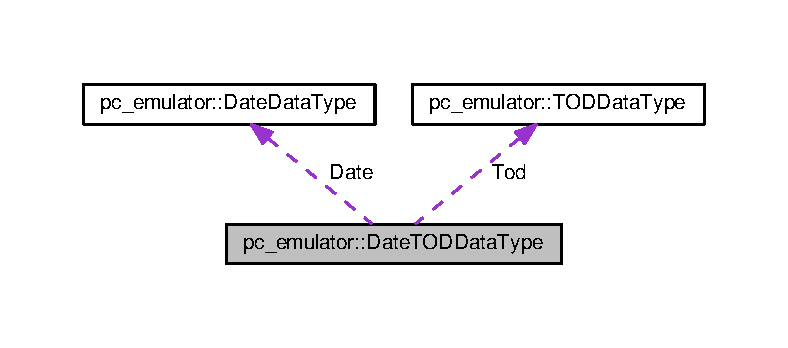
\includegraphics[width=350pt]{structpc__emulator_1_1DateTODDataType__coll__graph}
\end{center}
\end{figure}
\subsection*{Public Member Functions}
\begin{DoxyCompactItemize}
\item 
\hyperlink{structpc__emulator_1_1DateTODDataType}{Date\+T\+O\+D\+Data\+Type} \& \hyperlink{structpc__emulator_1_1DateTODDataType_ab10d6001d2511343ffdfccf674b40905}{operator+} (const \hyperlink{structpc__emulator_1_1DateTODDataType}{Date\+T\+O\+D\+Data\+Type} \&a)\hypertarget{structpc__emulator_1_1DateTODDataType_ab10d6001d2511343ffdfccf674b40905}{}\label{structpc__emulator_1_1DateTODDataType_ab10d6001d2511343ffdfccf674b40905}

\begin{DoxyCompactList}\small\item\em A\+DD operator for two dt data types. Does nothing. \end{DoxyCompactList}\item 
\hyperlink{structpc__emulator_1_1DateTODDataType}{Date\+T\+O\+D\+Data\+Type} \& \hyperlink{structpc__emulator_1_1DateTODDataType_abc7b4516ccd3d9865961909bbffc6f26}{operator-\/} (const \hyperlink{structpc__emulator_1_1DateTODDataType}{Date\+T\+O\+D\+Data\+Type} \&a)\hypertarget{structpc__emulator_1_1DateTODDataType_abc7b4516ccd3d9865961909bbffc6f26}{}\label{structpc__emulator_1_1DateTODDataType_abc7b4516ccd3d9865961909bbffc6f26}

\begin{DoxyCompactList}\small\item\em Sub operator for two dt data types. Does nothing. \end{DoxyCompactList}\item 
\hyperlink{structpc__emulator_1_1DateTODDataType}{Date\+T\+O\+D\+Data\+Type} \& \hyperlink{structpc__emulator_1_1DateTODDataType_a17b7d54b77f6bd0a5644cc027c465384}{operator/} (const \hyperlink{structpc__emulator_1_1DateTODDataType}{Date\+T\+O\+D\+Data\+Type} \&a)\hypertarget{structpc__emulator_1_1DateTODDataType_a17b7d54b77f6bd0a5644cc027c465384}{}\label{structpc__emulator_1_1DateTODDataType_a17b7d54b77f6bd0a5644cc027c465384}

\begin{DoxyCompactList}\small\item\em Divide operator for two dt data types. Does nothing. \end{DoxyCompactList}\item 
\hyperlink{structpc__emulator_1_1DateTODDataType}{Date\+T\+O\+D\+Data\+Type} \& \hyperlink{structpc__emulator_1_1DateTODDataType_a6ac922d5104336741eb6c5fe262ca0b4}{operator\%} (const \hyperlink{structpc__emulator_1_1DateTODDataType}{Date\+T\+O\+D\+Data\+Type} \&a)\hypertarget{structpc__emulator_1_1DateTODDataType_a6ac922d5104336741eb6c5fe262ca0b4}{}\label{structpc__emulator_1_1DateTODDataType_a6ac922d5104336741eb6c5fe262ca0b4}

\begin{DoxyCompactList}\small\item\em Mod operator for two dt data types. Does nothing. \end{DoxyCompactList}\item 
\hyperlink{structpc__emulator_1_1DateTODDataType}{Date\+T\+O\+D\+Data\+Type} \& \hyperlink{structpc__emulator_1_1DateTODDataType_a1663a50decfc0ab9d6313256aca42034}{operator$\ast$} (const \hyperlink{structpc__emulator_1_1DateTODDataType}{Date\+T\+O\+D\+Data\+Type} \&a)\hypertarget{structpc__emulator_1_1DateTODDataType_a1663a50decfc0ab9d6313256aca42034}{}\label{structpc__emulator_1_1DateTODDataType_a1663a50decfc0ab9d6313256aca42034}

\begin{DoxyCompactList}\small\item\em Multiply operator for two dt data types. Does nothing. \end{DoxyCompactList}\item 
\hyperlink{structpc__emulator_1_1DateTODDataType}{Date\+T\+O\+D\+Data\+Type} \& \hyperlink{structpc__emulator_1_1DateTODDataType_ab666f2a21b8ea87cd487e736c21bcf9d}{operator\&} (const \hyperlink{structpc__emulator_1_1DateTODDataType}{Date\+T\+O\+D\+Data\+Type} \&a)\hypertarget{structpc__emulator_1_1DateTODDataType_ab666f2a21b8ea87cd487e736c21bcf9d}{}\label{structpc__emulator_1_1DateTODDataType_ab666f2a21b8ea87cd487e736c21bcf9d}

\begin{DoxyCompactList}\small\item\em A\+ND operator for two dt data types. Does nothing. \end{DoxyCompactList}\item 
\hyperlink{structpc__emulator_1_1DateTODDataType}{Date\+T\+O\+D\+Data\+Type} \& \hyperlink{structpc__emulator_1_1DateTODDataType_a94d092afaa9a2dca6c650d6049cb9b35}{operator$\vert$} (const \hyperlink{structpc__emulator_1_1DateTODDataType}{Date\+T\+O\+D\+Data\+Type} \&a)\hypertarget{structpc__emulator_1_1DateTODDataType_a94d092afaa9a2dca6c650d6049cb9b35}{}\label{structpc__emulator_1_1DateTODDataType_a94d092afaa9a2dca6c650d6049cb9b35}

\begin{DoxyCompactList}\small\item\em OR operator for two dt data types. Does nothing. \end{DoxyCompactList}\item 
\hyperlink{structpc__emulator_1_1DateTODDataType}{Date\+T\+O\+D\+Data\+Type} \& \hyperlink{structpc__emulator_1_1DateTODDataType_a5332d6081bea88bcfad6477f39361bc7}{operator$^\wedge$} (const \hyperlink{structpc__emulator_1_1DateTODDataType}{Date\+T\+O\+D\+Data\+Type} \&a)\hypertarget{structpc__emulator_1_1DateTODDataType_a5332d6081bea88bcfad6477f39361bc7}{}\label{structpc__emulator_1_1DateTODDataType_a5332d6081bea88bcfad6477f39361bc7}

\begin{DoxyCompactList}\small\item\em X\+OR operator for two dt data types. Does nothing. \end{DoxyCompactList}\end{DoxyCompactItemize}
\subsection*{Public Attributes}
\begin{DoxyCompactItemize}
\item 
\hyperlink{structpc__emulator_1_1DateDataType}{Date\+Type} {\bfseries Date}\hypertarget{structpc__emulator_1_1DateTODDataType_a1e683832449d6ba64cf4b6b8f080c2e4}{}\label{structpc__emulator_1_1DateTODDataType_a1e683832449d6ba64cf4b6b8f080c2e4}

\item 
\hyperlink{structpc__emulator_1_1TODDataType}{T\+O\+D\+Type} {\bfseries Tod}\hypertarget{structpc__emulator_1_1DateTODDataType_a1db9a800fe40945e22115ef337179179}{}\label{structpc__emulator_1_1DateTODDataType_a1db9a800fe40945e22115ef337179179}

\end{DoxyCompactItemize}
\subsection*{Friends}
\begin{DoxyCompactItemize}
\item 
bool \hyperlink{structpc__emulator_1_1DateTODDataType_a19e48a0fa1dfbad95a2cde6a4e9d9a8f}{operator$<$} (const \hyperlink{structpc__emulator_1_1DateTODDataType}{Date\+T\+O\+D\+Data\+Type} \&b, const \hyperlink{structpc__emulator_1_1DateTODDataType}{Date\+T\+O\+D\+Data\+Type} \&a)\hypertarget{structpc__emulator_1_1DateTODDataType_a19e48a0fa1dfbad95a2cde6a4e9d9a8f}{}\label{structpc__emulator_1_1DateTODDataType_a19e48a0fa1dfbad95a2cde6a4e9d9a8f}

\begin{DoxyCompactList}\small\item\em Less than operator for two dt data types. \end{DoxyCompactList}\item 
bool \hyperlink{structpc__emulator_1_1DateTODDataType_a8a4ba8113332a3ada78f1cdfd91c828f}{operator$<$=} (const \hyperlink{structpc__emulator_1_1DateTODDataType}{Date\+T\+O\+D\+Data\+Type} \&b, const \hyperlink{structpc__emulator_1_1DateTODDataType}{Date\+T\+O\+D\+Data\+Type} \&a)\hypertarget{structpc__emulator_1_1DateTODDataType_a8a4ba8113332a3ada78f1cdfd91c828f}{}\label{structpc__emulator_1_1DateTODDataType_a8a4ba8113332a3ada78f1cdfd91c828f}

\begin{DoxyCompactList}\small\item\em Less than or equal operator for two dt data types. \end{DoxyCompactList}\item 
bool \hyperlink{structpc__emulator_1_1DateTODDataType_a3f3ead1153a14c1d7806acb8486d14c0}{operator$>$} (const \hyperlink{structpc__emulator_1_1DateTODDataType}{Date\+T\+O\+D\+Data\+Type} \&b, const \hyperlink{structpc__emulator_1_1DateTODDataType}{Date\+T\+O\+D\+Data\+Type} \&a)\hypertarget{structpc__emulator_1_1DateTODDataType_a3f3ead1153a14c1d7806acb8486d14c0}{}\label{structpc__emulator_1_1DateTODDataType_a3f3ead1153a14c1d7806acb8486d14c0}

\begin{DoxyCompactList}\small\item\em Greater than operator for two dt data types. \end{DoxyCompactList}\item 
bool \hyperlink{structpc__emulator_1_1DateTODDataType_ac13253f7b93b0c57e0d3408aa42b70bc}{operator$>$=} (const \hyperlink{structpc__emulator_1_1DateTODDataType}{Date\+T\+O\+D\+Data\+Type} \&b, const \hyperlink{structpc__emulator_1_1DateTODDataType}{Date\+T\+O\+D\+Data\+Type} \&a)\hypertarget{structpc__emulator_1_1DateTODDataType_ac13253f7b93b0c57e0d3408aa42b70bc}{}\label{structpc__emulator_1_1DateTODDataType_ac13253f7b93b0c57e0d3408aa42b70bc}

\begin{DoxyCompactList}\small\item\em Greater than or equal operator for two dt data types. \end{DoxyCompactList}\item 
bool {\bfseries operator==} (const \hyperlink{structpc__emulator_1_1DateTODDataType}{Date\+T\+O\+D\+Data\+Type} \&b, const \hyperlink{structpc__emulator_1_1DateTODDataType}{Date\+T\+O\+D\+Data\+Type} \&a)\hypertarget{structpc__emulator_1_1DateTODDataType_a61e8dac6a0bb3bde076ce024ae4de7f1}{}\label{structpc__emulator_1_1DateTODDataType_a61e8dac6a0bb3bde076ce024ae4de7f1}

\end{DoxyCompactItemize}


\subsection{Detailed Description}
Date and Time (dt) data type. 

The documentation for this struct was generated from the following file\+:\begin{DoxyCompactItemize}
\item 
src/pc\+\_\+emulator/include/elementary\+\_\+datatypes.\+h\end{DoxyCompactItemize}

\hypertarget{classpc__emulator_1_1DIV__Insn}{}\section{pc\+\_\+emulator\+:\+:D\+I\+V\+\_\+\+Insn Class Reference}
\label{classpc__emulator_1_1DIV__Insn}\index{pc\+\_\+emulator\+::\+D\+I\+V\+\_\+\+Insn@{pc\+\_\+emulator\+::\+D\+I\+V\+\_\+\+Insn}}


D\+IV instruction.  




{\ttfamily \#include $<$div\+\_\+insn.\+h$>$}



Inheritance diagram for pc\+\_\+emulator\+:\+:D\+I\+V\+\_\+\+Insn\+:
\nopagebreak
\begin{figure}[H]
\begin{center}
\leavevmode
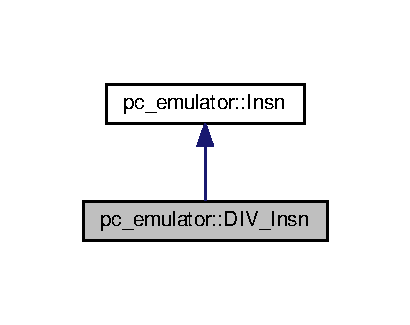
\includegraphics[width=197pt]{classpc__emulator_1_1DIV__Insn__inherit__graph}
\end{center}
\end{figure}


Collaboration diagram for pc\+\_\+emulator\+:\+:D\+I\+V\+\_\+\+Insn\+:
\nopagebreak
\begin{figure}[H]
\begin{center}
\leavevmode
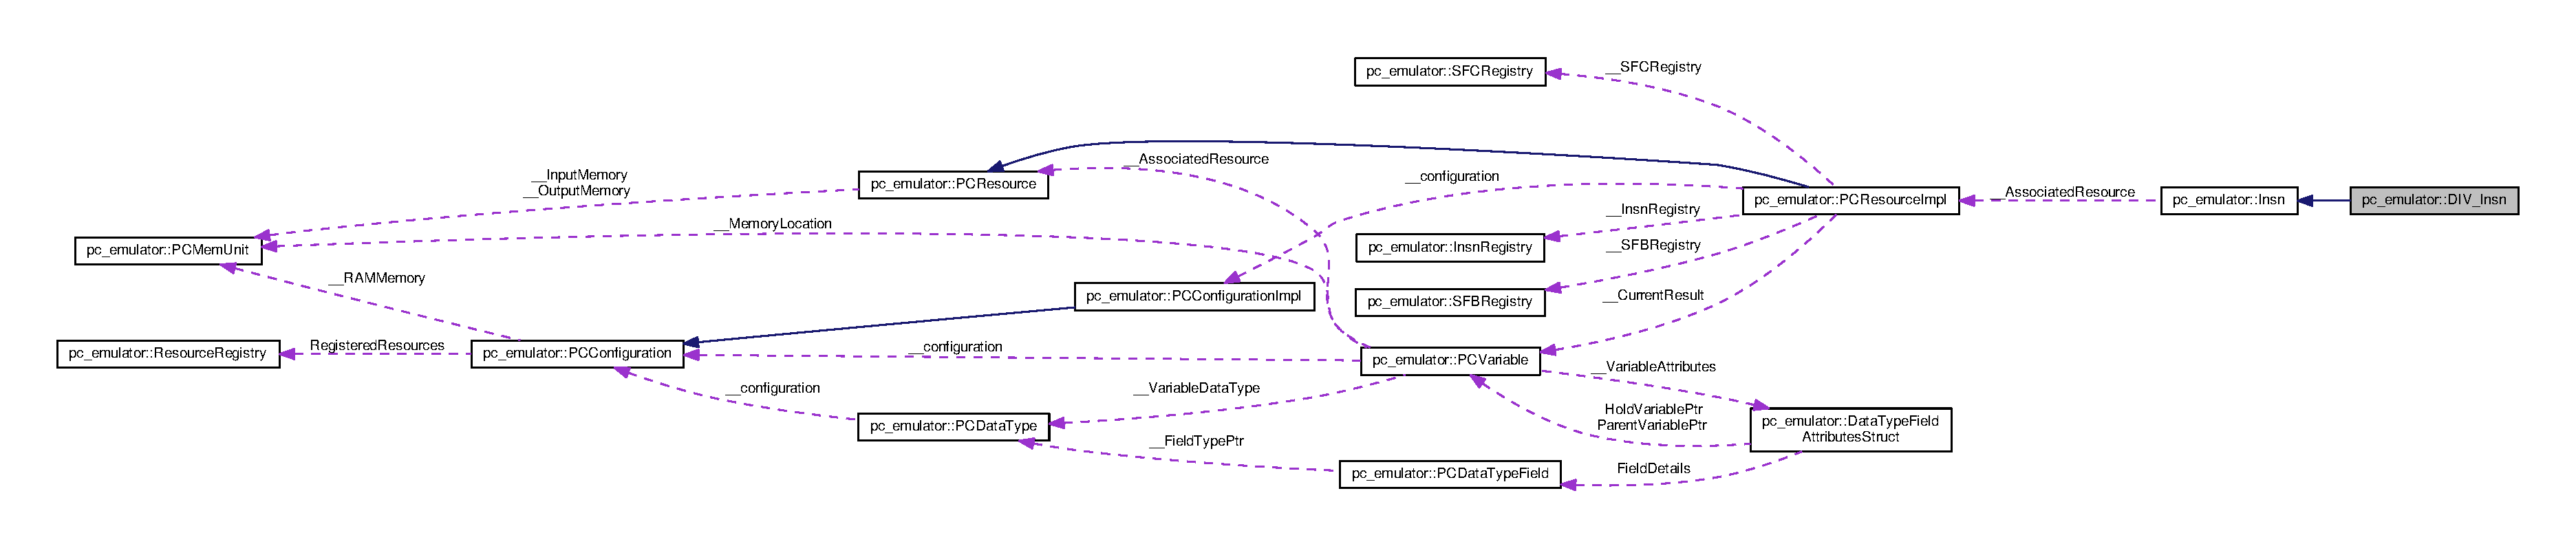
\includegraphics[width=350pt]{classpc__emulator_1_1DIV__Insn__coll__graph}
\end{center}
\end{figure}
\subsection*{Public Member Functions}
\begin{DoxyCompactItemize}
\item 
{\bfseries D\+I\+V\+\_\+\+Insn} (\hyperlink{classpc__emulator_1_1PCResourceImpl}{P\+C\+Resource\+Impl} $\ast$Associated\+Resource, bool is\+Negated)\hypertarget{classpc__emulator_1_1DIV__Insn_a6209c51bdc5d28284213b8859de646b5}{}\label{classpc__emulator_1_1DIV__Insn_a6209c51bdc5d28284213b8859de646b5}

\item 
void \hyperlink{classpc__emulator_1_1DIV__Insn_a25e0da13e7b4ea49277ba62854382c8d}{Execute} (\hyperlink{classpc__emulator_1_1PCVariable}{P\+C\+Variable} $\ast$Current\+Result, std\+::vector$<$ \hyperlink{classpc__emulator_1_1PCVariable}{P\+C\+Variable} $\ast$ $>$ \&Operands)
\begin{DoxyCompactList}\small\item\em Called to execute the instruction. \end{DoxyCompactList}\end{DoxyCompactItemize}
\subsection*{Additional Inherited Members}


\subsection{Detailed Description}
D\+IV instruction. 

\subsection{Member Function Documentation}
\index{pc\+\_\+emulator\+::\+D\+I\+V\+\_\+\+Insn@{pc\+\_\+emulator\+::\+D\+I\+V\+\_\+\+Insn}!Execute@{Execute}}
\index{Execute@{Execute}!pc\+\_\+emulator\+::\+D\+I\+V\+\_\+\+Insn@{pc\+\_\+emulator\+::\+D\+I\+V\+\_\+\+Insn}}
\subsubsection[{\texorpdfstring{Execute(\+P\+C\+Variable $\ast$\+Current\+Result, std\+::vector$<$ P\+C\+Variable $\ast$ $>$ \&\+Operands)}{Execute(PCVariable *CurrentResult, std::vector< PCVariable * > &Operands)}}]{\setlength{\rightskip}{0pt plus 5cm}void pc\+\_\+emulator\+::\+D\+I\+V\+\_\+\+Insn\+::\+Execute (
\begin{DoxyParamCaption}
\item[{{\bf P\+C\+Variable} $\ast$}]{Current\+Result, }
\item[{std\+::vector$<$ {\bf P\+C\+Variable} $\ast$ $>$ \&}]{Operands}
\end{DoxyParamCaption}
)\hspace{0.3cm}{\ttfamily [virtual]}}\hypertarget{classpc__emulator_1_1DIV__Insn_a25e0da13e7b4ea49277ba62854382c8d}{}\label{classpc__emulator_1_1DIV__Insn_a25e0da13e7b4ea49277ba62854382c8d}


Called to execute the instruction. 


\begin{DoxyParams}{Parameters}
{\em Current\+Result} & The Current\+Result register of the task executing this \hyperlink{classpc__emulator_1_1Insn}{Insn} \\
\hline
{\em Operands} & Operands to the instruction \\
\hline
\end{DoxyParams}


Implements \hyperlink{classpc__emulator_1_1Insn_a103d27030e872a799e313df16c1f3d66}{pc\+\_\+emulator\+::\+Insn}.



The documentation for this class was generated from the following file\+:\begin{DoxyCompactItemize}
\item 
src/pc\+\_\+emulator/include/insns/div\+\_\+insn.\+h\end{DoxyCompactItemize}

\hypertarget{classpc__emulator_1_1EQ__Insn}{}\section{pc\+\_\+emulator\+:\+:E\+Q\+\_\+\+Insn Class Reference}
\label{classpc__emulator_1_1EQ__Insn}\index{pc\+\_\+emulator\+::\+E\+Q\+\_\+\+Insn@{pc\+\_\+emulator\+::\+E\+Q\+\_\+\+Insn}}


Equality checking instruction.  




{\ttfamily \#include $<$eq\+\_\+insn.\+h$>$}



Inheritance diagram for pc\+\_\+emulator\+:\+:E\+Q\+\_\+\+Insn\+:
\nopagebreak
\begin{figure}[H]
\begin{center}
\leavevmode
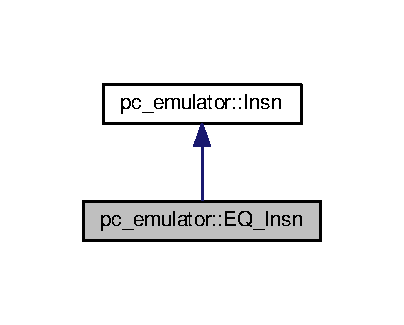
\includegraphics[width=194pt]{classpc__emulator_1_1EQ__Insn__inherit__graph}
\end{center}
\end{figure}


Collaboration diagram for pc\+\_\+emulator\+:\+:E\+Q\+\_\+\+Insn\+:
\nopagebreak
\begin{figure}[H]
\begin{center}
\leavevmode
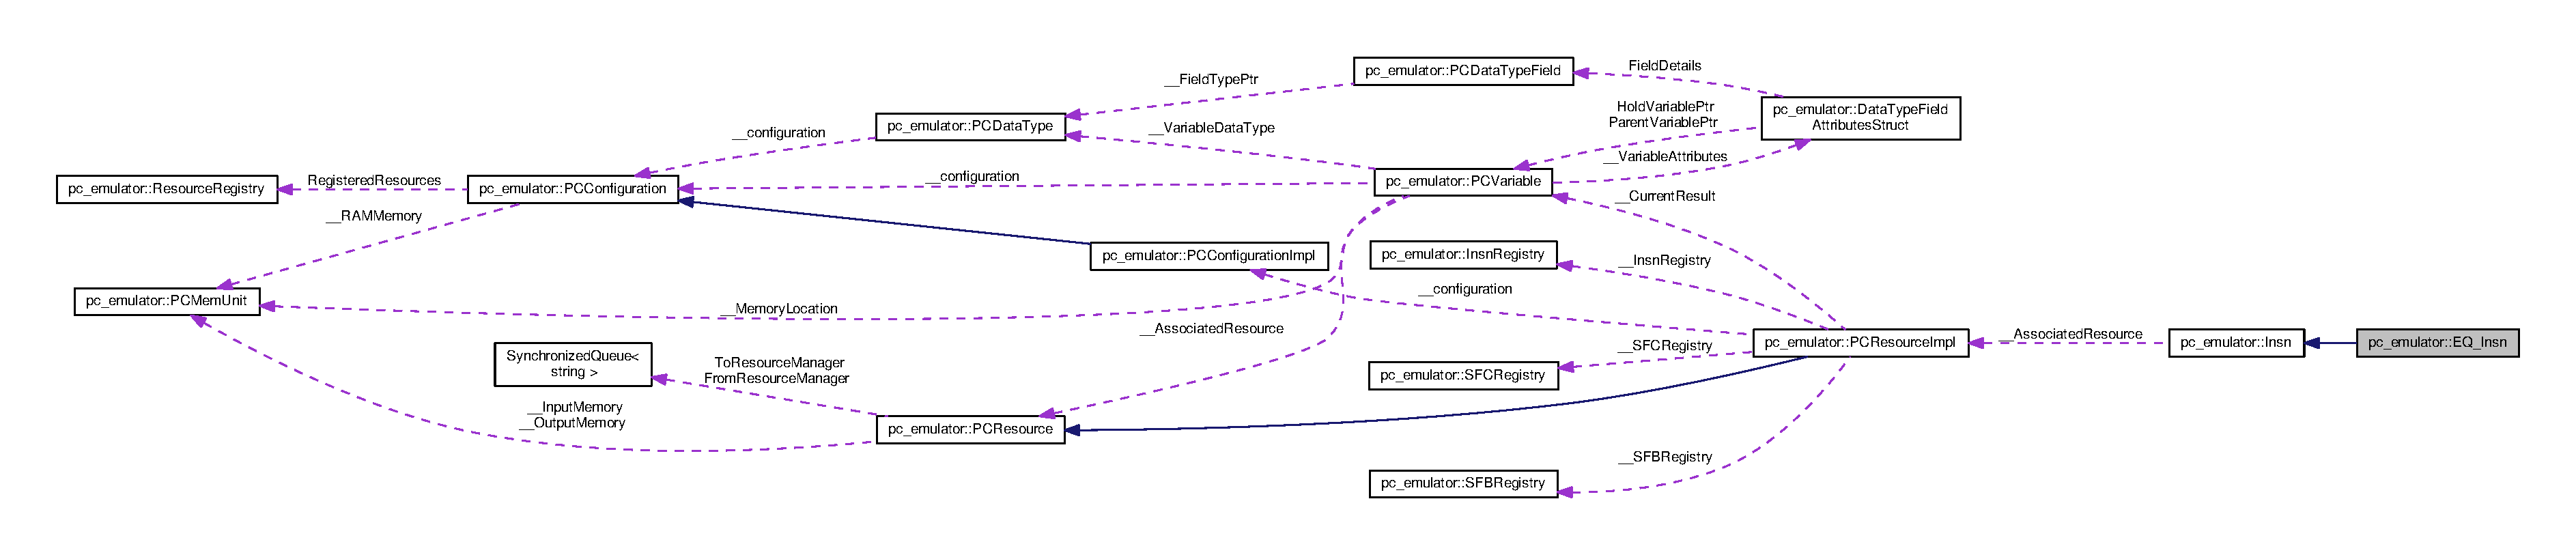
\includegraphics[width=350pt]{classpc__emulator_1_1EQ__Insn__coll__graph}
\end{center}
\end{figure}
\subsection*{Public Member Functions}
\begin{DoxyCompactItemize}
\item 
{\bfseries E\+Q\+\_\+\+Insn} (\hyperlink{classpc__emulator_1_1PCResourceImpl}{P\+C\+Resource\+Impl} $\ast$Associated\+Resource, bool is\+Negated)\hypertarget{classpc__emulator_1_1EQ__Insn_a5c8e3fb27650e6cd02432608e3fe590a}{}\label{classpc__emulator_1_1EQ__Insn_a5c8e3fb27650e6cd02432608e3fe590a}

\item 
void \hyperlink{classpc__emulator_1_1EQ__Insn_ac0337e98a5bef35cf38880caa03969ed}{Execute} (\hyperlink{classpc__emulator_1_1PCVariable}{P\+C\+Variable} $\ast$Current\+Result, std\+::vector$<$ \hyperlink{classpc__emulator_1_1PCVariable}{P\+C\+Variable} $\ast$ $>$ \&Operands)
\begin{DoxyCompactList}\small\item\em Called to execute the instruction. \end{DoxyCompactList}\end{DoxyCompactItemize}
\subsection*{Additional Inherited Members}


\subsection{Detailed Description}
Equality checking instruction. 

\subsection{Member Function Documentation}
\index{pc\+\_\+emulator\+::\+E\+Q\+\_\+\+Insn@{pc\+\_\+emulator\+::\+E\+Q\+\_\+\+Insn}!Execute@{Execute}}
\index{Execute@{Execute}!pc\+\_\+emulator\+::\+E\+Q\+\_\+\+Insn@{pc\+\_\+emulator\+::\+E\+Q\+\_\+\+Insn}}
\subsubsection[{\texorpdfstring{Execute(\+P\+C\+Variable $\ast$\+Current\+Result, std\+::vector$<$ P\+C\+Variable $\ast$ $>$ \&\+Operands)}{Execute(PCVariable *CurrentResult, std::vector< PCVariable * > &Operands)}}]{\setlength{\rightskip}{0pt plus 5cm}void pc\+\_\+emulator\+::\+E\+Q\+\_\+\+Insn\+::\+Execute (
\begin{DoxyParamCaption}
\item[{{\bf P\+C\+Variable} $\ast$}]{Current\+Result, }
\item[{std\+::vector$<$ {\bf P\+C\+Variable} $\ast$ $>$ \&}]{Operands}
\end{DoxyParamCaption}
)\hspace{0.3cm}{\ttfamily [virtual]}}\hypertarget{classpc__emulator_1_1EQ__Insn_ac0337e98a5bef35cf38880caa03969ed}{}\label{classpc__emulator_1_1EQ__Insn_ac0337e98a5bef35cf38880caa03969ed}


Called to execute the instruction. 


\begin{DoxyParams}{Parameters}
{\em Current\+Result} & The Current\+Result register of the task executing this \hyperlink{classpc__emulator_1_1Insn}{Insn} \\
\hline
{\em Operands} & Operands to the instruction \\
\hline
\end{DoxyParams}


Implements \hyperlink{classpc__emulator_1_1Insn_a103d27030e872a799e313df16c1f3d66}{pc\+\_\+emulator\+::\+Insn}.



The documentation for this class was generated from the following file\+:\begin{DoxyCompactItemize}
\item 
src/pc\+\_\+emulator/include/insns/eq\+\_\+insn.\+h\end{DoxyCompactItemize}

\hypertarget{classpc__emulator_1_1Executor}{}\section{pc\+\_\+emulator\+:\+:Executor Class Reference}
\label{classpc__emulator_1_1Executor}\index{pc\+\_\+emulator\+::\+Executor@{pc\+\_\+emulator\+::\+Executor}}


Collaboration diagram for pc\+\_\+emulator\+:\+:Executor\+:
\nopagebreak
\begin{figure}[H]
\begin{center}
\leavevmode
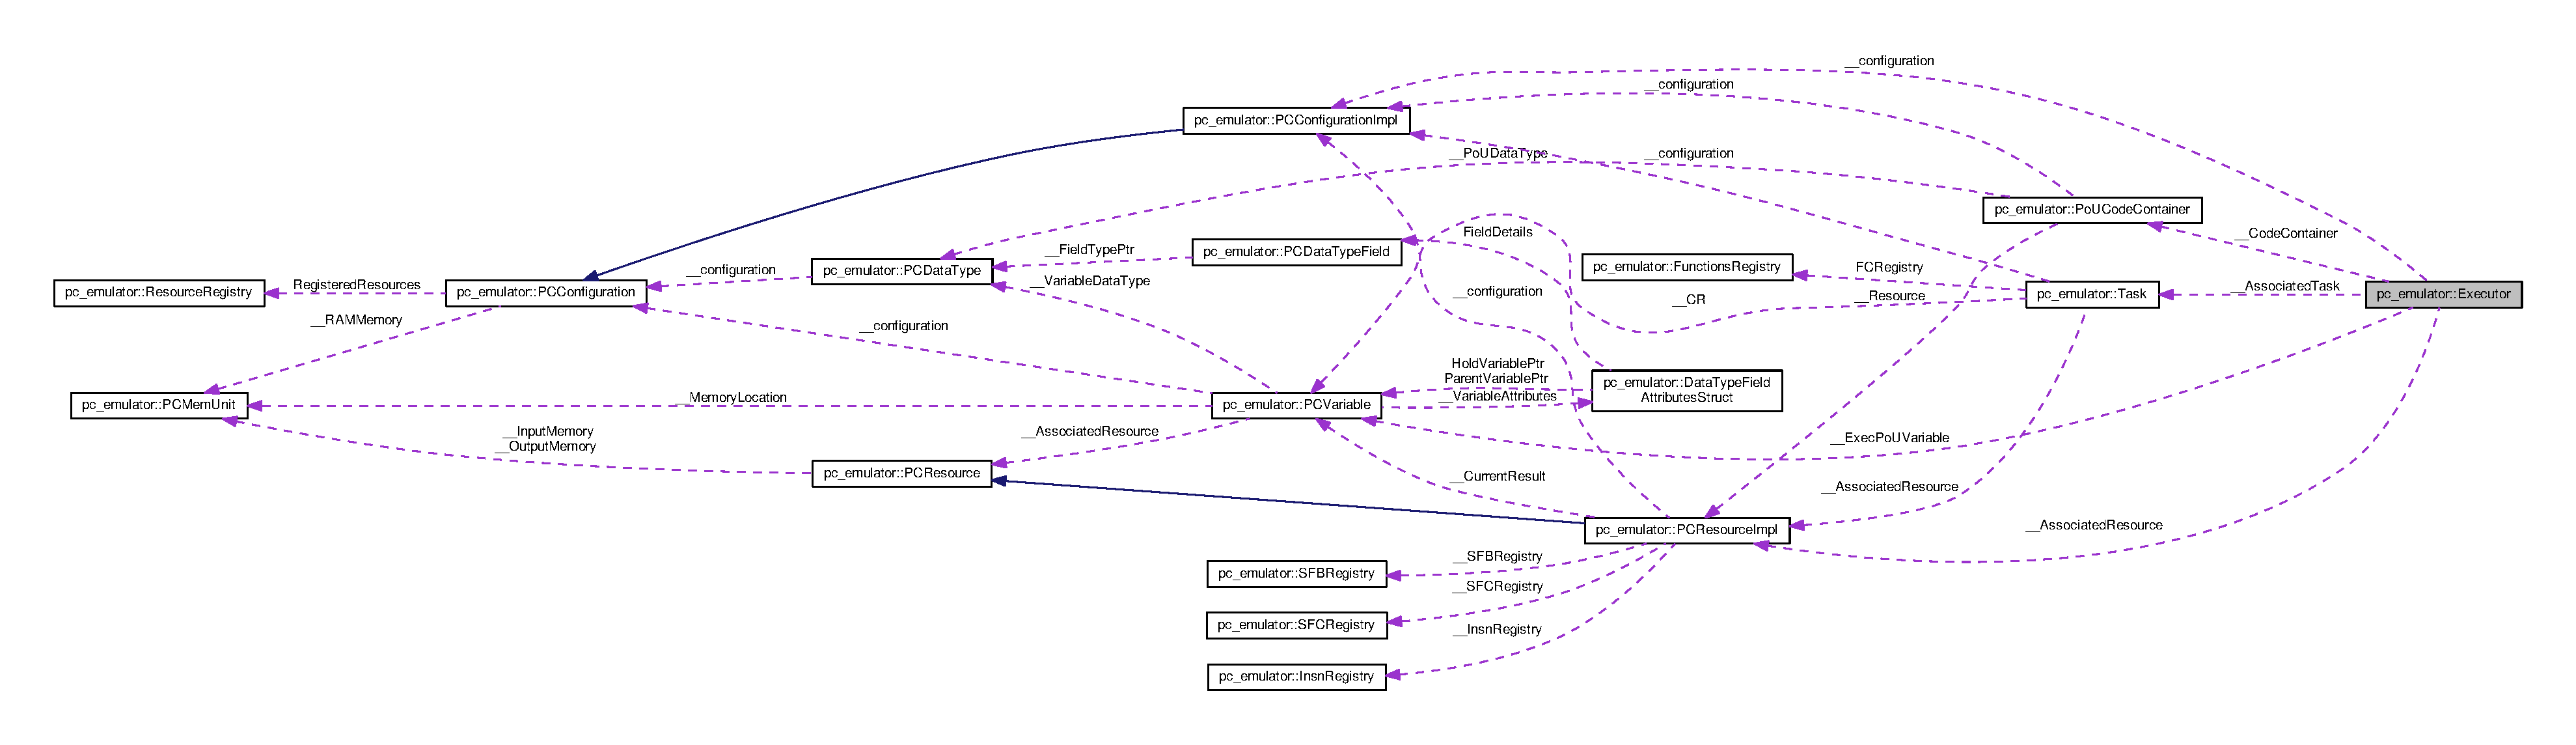
\includegraphics[width=350pt]{classpc__emulator_1_1Executor__coll__graph}
\end{center}
\end{figure}
\subsection*{Public Member Functions}
\begin{DoxyCompactItemize}
\item 
\hyperlink{classpc__emulator_1_1Executor_a55e78f5999c4ba3648a66927426a51d0}{Executor} (\hyperlink{classpc__emulator_1_1PCConfigurationImpl}{P\+C\+Configuration\+Impl} $\ast$configuration, \hyperlink{classpc__emulator_1_1PCResourceImpl}{P\+C\+Resource\+Impl} $\ast$Associated\+Resource, \hyperlink{classpc__emulator_1_1Task}{Task} $\ast$Associated\+Task)
\begin{DoxyCompactList}\small\item\em Constructor. \end{DoxyCompactList}\item 
void \hyperlink{classpc__emulator_1_1Executor_a2dbf56b19f3fbaf775f7b33b50ec8de9}{Set\+Exec\+Po\+U\+Variable} (\hyperlink{classpc__emulator_1_1PCVariable}{P\+C\+Variable} $\ast$Exec\+Po\+U\+Variable)
\begin{DoxyCompactList}\small\item\em Sets a PoU to this executor. \end{DoxyCompactList}\item 
void \hyperlink{classpc__emulator_1_1Executor_a2fd64c8278fe4cb4b3040c1f1cc0c874}{Run} ()\hypertarget{classpc__emulator_1_1Executor_a2fd64c8278fe4cb4b3040c1f1cc0c874}{}\label{classpc__emulator_1_1Executor_a2fd64c8278fe4cb4b3040c1f1cc0c874}

\begin{DoxyCompactList}\small\item\em Runs the executor. Starts running each instruction. \end{DoxyCompactList}\item 
void \hyperlink{classpc__emulator_1_1Executor_a8bbf346063821d7a9c5e9b734f29a70f}{Clean\+Up} ()\hypertarget{classpc__emulator_1_1Executor_a8bbf346063821d7a9c5e9b734f29a70f}{}\label{classpc__emulator_1_1Executor_a8bbf346063821d7a9c5e9b734f29a70f}

\begin{DoxyCompactList}\small\item\em Cleanup and do other book keeping. \end{DoxyCompactList}\item 
int \hyperlink{classpc__emulator_1_1Executor_abf2af6604c54863a1a67a36a2526e357}{Run\+Insn} (\hyperlink{classpc__emulator_1_1InsnContainer}{Insn\+Container} \&insn\+\_\+container)
\begin{DoxyCompactList}\small\item\em Runs the current instruction and returns idx of next instruction to execute. \end{DoxyCompactList}\item 
void \hyperlink{classpc__emulator_1_1Executor_ad1bfe0eefa104d73193b062270e83008}{Save\+C\+P\+U\+Registers} ()\hypertarget{classpc__emulator_1_1Executor_ad1bfe0eefa104d73193b062270e83008}{}\label{classpc__emulator_1_1Executor_ad1bfe0eefa104d73193b062270e83008}

\begin{DoxyCompactList}\small\item\em Saves the current result register of the resource. \end{DoxyCompactList}\item 
void \hyperlink{classpc__emulator_1_1Executor_af20b7d1a162e6b974ff228c51ea86d92}{Restore\+C\+P\+U\+Registers} ()\hypertarget{classpc__emulator_1_1Executor_af20b7d1a162e6b974ff228c51ea86d92}{}\label{classpc__emulator_1_1Executor_af20b7d1a162e6b974ff228c51ea86d92}

\begin{DoxyCompactList}\small\item\em Restores the current result register of the resource. \end{DoxyCompactList}\item 
void \hyperlink{classpc__emulator_1_1Executor_ae735d64520122eff70a5f539375027e6}{Reset\+C\+P\+U\+Registers} ()\hypertarget{classpc__emulator_1_1Executor_ae735d64520122eff70a5f539375027e6}{}\label{classpc__emulator_1_1Executor_ae735d64520122eff70a5f539375027e6}

\begin{DoxyCompactList}\small\item\em Resets the current result register of the resource. \end{DoxyCompactList}\end{DoxyCompactItemize}
\subsection*{Public Attributes}
\begin{DoxyCompactItemize}
\item 
\hyperlink{classpc__emulator_1_1PCConfigurationImpl}{P\+C\+Configuration\+Impl} $\ast$ \hyperlink{classpc__emulator_1_1Executor_abcffb5c87513b158451390af932327e6}{\+\_\+\+\_\+configuration}
\item 
\hyperlink{classpc__emulator_1_1PCVariable}{P\+C\+Variable} $\ast$ \hyperlink{classpc__emulator_1_1Executor_a5b88e4a18e03884a98ae194c40d08803}{\+\_\+\+\_\+\+Exec\+Po\+U\+Variable}
\item 
\hyperlink{classpc__emulator_1_1PCResourceImpl}{P\+C\+Resource\+Impl} $\ast$ \hyperlink{classpc__emulator_1_1Executor_a08c9e456c5329834f50141d7add91a9f}{\+\_\+\+\_\+\+Associated\+Resource}
\item 
\hyperlink{classpc__emulator_1_1PoUCodeContainer}{Po\+U\+Code\+Container} $\ast$ \hyperlink{classpc__emulator_1_1Executor_a26032bb8f4fec484e14f32d07db89f5d}{\+\_\+\+\_\+\+Code\+Container}
\item 
bool \hyperlink{classpc__emulator_1_1Executor_a8c58feead8d23b32927237f2f6fc5c7a}{\+\_\+\+\_\+\+Initialized}
\item 
\hyperlink{classpc__emulator_1_1Task}{Task} $\ast$ \hyperlink{classpc__emulator_1_1Executor_ac1f6ee2ee941691f69f0d51827fd2a06}{\+\_\+\+\_\+\+Associated\+Task}
\item 
\hyperlink{classpc__emulator_1_1PCVariable}{P\+C\+Variable} $\ast$ {\bfseries \+\_\+\+\_\+\+CR}\hypertarget{classpc__emulator_1_1Executor_a9946f739f53375d187386eebc60a174c}{}\label{classpc__emulator_1_1Executor_a9946f739f53375d187386eebc60a174c}

\end{DoxyCompactItemize}


\subsection{Constructor \& Destructor Documentation}
\index{pc\+\_\+emulator\+::\+Executor@{pc\+\_\+emulator\+::\+Executor}!Executor@{Executor}}
\index{Executor@{Executor}!pc\+\_\+emulator\+::\+Executor@{pc\+\_\+emulator\+::\+Executor}}
\subsubsection[{\texorpdfstring{Executor(\+P\+C\+Configuration\+Impl $\ast$configuration, P\+C\+Resource\+Impl $\ast$\+Associated\+Resource, Task $\ast$\+Associated\+Task)}{Executor(PCConfigurationImpl *configuration, PCResourceImpl *AssociatedResource, Task *AssociatedTask)}}]{\setlength{\rightskip}{0pt plus 5cm}pc\+\_\+emulator\+::\+Executor\+::\+Executor (
\begin{DoxyParamCaption}
\item[{{\bf P\+C\+Configuration\+Impl} $\ast$}]{configuration, }
\item[{{\bf P\+C\+Resource\+Impl} $\ast$}]{Associated\+Resource, }
\item[{{\bf Task} $\ast$}]{Associated\+Task}
\end{DoxyParamCaption}
)\hspace{0.3cm}{\ttfamily [inline]}}\hypertarget{classpc__emulator_1_1Executor_a55e78f5999c4ba3648a66927426a51d0}{}\label{classpc__emulator_1_1Executor_a55e78f5999c4ba3648a66927426a51d0}


Constructor. 

local copy of the current result register of the associated resource 

\subsection{Member Function Documentation}
\index{pc\+\_\+emulator\+::\+Executor@{pc\+\_\+emulator\+::\+Executor}!Run\+Insn@{Run\+Insn}}
\index{Run\+Insn@{Run\+Insn}!pc\+\_\+emulator\+::\+Executor@{pc\+\_\+emulator\+::\+Executor}}
\subsubsection[{\texorpdfstring{Run\+Insn(\+Insn\+Container \&insn\+\_\+container)}{RunInsn(InsnContainer &insn_container)}}]{\setlength{\rightskip}{0pt plus 5cm}int pc\+\_\+emulator\+::\+Executor\+::\+Run\+Insn (
\begin{DoxyParamCaption}
\item[{{\bf Insn\+Container} \&}]{insn\+\_\+container}
\end{DoxyParamCaption}
)}\hypertarget{classpc__emulator_1_1Executor_abf2af6604c54863a1a67a36a2526e357}{}\label{classpc__emulator_1_1Executor_abf2af6604c54863a1a67a36a2526e357}


Runs the current instruction and returns idx of next instruction to execute. 


\begin{DoxyParams}{Parameters}
{\em insn\+\_\+container} & Current instruction to execute \\
\hline
\end{DoxyParams}
\begin{DoxyReturn}{Returns}
idx of next instruction to execute 
\end{DoxyReturn}
\index{pc\+\_\+emulator\+::\+Executor@{pc\+\_\+emulator\+::\+Executor}!Set\+Exec\+Po\+U\+Variable@{Set\+Exec\+Po\+U\+Variable}}
\index{Set\+Exec\+Po\+U\+Variable@{Set\+Exec\+Po\+U\+Variable}!pc\+\_\+emulator\+::\+Executor@{pc\+\_\+emulator\+::\+Executor}}
\subsubsection[{\texorpdfstring{Set\+Exec\+Po\+U\+Variable(\+P\+C\+Variable $\ast$\+Exec\+Po\+U\+Variable)}{SetExecPoUVariable(PCVariable *ExecPoUVariable)}}]{\setlength{\rightskip}{0pt plus 5cm}void pc\+\_\+emulator\+::\+Executor\+::\+Set\+Exec\+Po\+U\+Variable (
\begin{DoxyParamCaption}
\item[{{\bf P\+C\+Variable} $\ast$}]{Exec\+Po\+U\+Variable}
\end{DoxyParamCaption}
)}\hypertarget{classpc__emulator_1_1Executor_a2dbf56b19f3fbaf775f7b33b50ec8de9}{}\label{classpc__emulator_1_1Executor_a2dbf56b19f3fbaf775f7b33b50ec8de9}


Sets a PoU to this executor. 


\begin{DoxyParams}{Parameters}
{\em Exec\+Po\+U\+Variable} & PoU to be assigned to this executor \\
\hline
\end{DoxyParams}


\subsection{Member Data Documentation}
\index{pc\+\_\+emulator\+::\+Executor@{pc\+\_\+emulator\+::\+Executor}!\+\_\+\+\_\+\+Associated\+Resource@{\+\_\+\+\_\+\+Associated\+Resource}}
\index{\+\_\+\+\_\+\+Associated\+Resource@{\+\_\+\+\_\+\+Associated\+Resource}!pc\+\_\+emulator\+::\+Executor@{pc\+\_\+emulator\+::\+Executor}}
\subsubsection[{\texorpdfstring{\+\_\+\+\_\+\+Associated\+Resource}{__AssociatedResource}}]{\setlength{\rightskip}{0pt plus 5cm}{\bf P\+C\+Resource\+Impl}$\ast$ pc\+\_\+emulator\+::\+Executor\+::\+\_\+\+\_\+\+Associated\+Resource}\hypertarget{classpc__emulator_1_1Executor_a08c9e456c5329834f50141d7add91a9f}{}\label{classpc__emulator_1_1Executor_a08c9e456c5329834f50141d7add91a9f}
Associated resource \index{pc\+\_\+emulator\+::\+Executor@{pc\+\_\+emulator\+::\+Executor}!\+\_\+\+\_\+\+Associated\+Task@{\+\_\+\+\_\+\+Associated\+Task}}
\index{\+\_\+\+\_\+\+Associated\+Task@{\+\_\+\+\_\+\+Associated\+Task}!pc\+\_\+emulator\+::\+Executor@{pc\+\_\+emulator\+::\+Executor}}
\subsubsection[{\texorpdfstring{\+\_\+\+\_\+\+Associated\+Task}{__AssociatedTask}}]{\setlength{\rightskip}{0pt plus 5cm}{\bf Task}$\ast$ pc\+\_\+emulator\+::\+Executor\+::\+\_\+\+\_\+\+Associated\+Task}\hypertarget{classpc__emulator_1_1Executor_ac1f6ee2ee941691f69f0d51827fd2a06}{}\label{classpc__emulator_1_1Executor_ac1f6ee2ee941691f69f0d51827fd2a06}
\hyperlink{classpc__emulator_1_1Task}{Task} associated with this executor \index{pc\+\_\+emulator\+::\+Executor@{pc\+\_\+emulator\+::\+Executor}!\+\_\+\+\_\+\+Code\+Container@{\+\_\+\+\_\+\+Code\+Container}}
\index{\+\_\+\+\_\+\+Code\+Container@{\+\_\+\+\_\+\+Code\+Container}!pc\+\_\+emulator\+::\+Executor@{pc\+\_\+emulator\+::\+Executor}}
\subsubsection[{\texorpdfstring{\+\_\+\+\_\+\+Code\+Container}{__CodeContainer}}]{\setlength{\rightskip}{0pt plus 5cm}{\bf Po\+U\+Code\+Container}$\ast$ pc\+\_\+emulator\+::\+Executor\+::\+\_\+\+\_\+\+Code\+Container}\hypertarget{classpc__emulator_1_1Executor_a26032bb8f4fec484e14f32d07db89f5d}{}\label{classpc__emulator_1_1Executor_a26032bb8f4fec484e14f32d07db89f5d}
Instructions of the PoU \index{pc\+\_\+emulator\+::\+Executor@{pc\+\_\+emulator\+::\+Executor}!\+\_\+\+\_\+configuration@{\+\_\+\+\_\+configuration}}
\index{\+\_\+\+\_\+configuration@{\+\_\+\+\_\+configuration}!pc\+\_\+emulator\+::\+Executor@{pc\+\_\+emulator\+::\+Executor}}
\subsubsection[{\texorpdfstring{\+\_\+\+\_\+configuration}{__configuration}}]{\setlength{\rightskip}{0pt plus 5cm}{\bf P\+C\+Configuration\+Impl}$\ast$ pc\+\_\+emulator\+::\+Executor\+::\+\_\+\+\_\+configuration}\hypertarget{classpc__emulator_1_1Executor_abcffb5c87513b158451390af932327e6}{}\label{classpc__emulator_1_1Executor_abcffb5c87513b158451390af932327e6}
Associated configuration \index{pc\+\_\+emulator\+::\+Executor@{pc\+\_\+emulator\+::\+Executor}!\+\_\+\+\_\+\+Exec\+Po\+U\+Variable@{\+\_\+\+\_\+\+Exec\+Po\+U\+Variable}}
\index{\+\_\+\+\_\+\+Exec\+Po\+U\+Variable@{\+\_\+\+\_\+\+Exec\+Po\+U\+Variable}!pc\+\_\+emulator\+::\+Executor@{pc\+\_\+emulator\+::\+Executor}}
\subsubsection[{\texorpdfstring{\+\_\+\+\_\+\+Exec\+Po\+U\+Variable}{__ExecPoUVariable}}]{\setlength{\rightskip}{0pt plus 5cm}{\bf P\+C\+Variable}$\ast$ pc\+\_\+emulator\+::\+Executor\+::\+\_\+\+\_\+\+Exec\+Po\+U\+Variable}\hypertarget{classpc__emulator_1_1Executor_a5b88e4a18e03884a98ae194c40d08803}{}\label{classpc__emulator_1_1Executor_a5b88e4a18e03884a98ae194c40d08803}
PoU to be executed \index{pc\+\_\+emulator\+::\+Executor@{pc\+\_\+emulator\+::\+Executor}!\+\_\+\+\_\+\+Initialized@{\+\_\+\+\_\+\+Initialized}}
\index{\+\_\+\+\_\+\+Initialized@{\+\_\+\+\_\+\+Initialized}!pc\+\_\+emulator\+::\+Executor@{pc\+\_\+emulator\+::\+Executor}}
\subsubsection[{\texorpdfstring{\+\_\+\+\_\+\+Initialized}{__Initialized}}]{\setlength{\rightskip}{0pt plus 5cm}bool pc\+\_\+emulator\+::\+Executor\+::\+\_\+\+\_\+\+Initialized}\hypertarget{classpc__emulator_1_1Executor_a8c58feead8d23b32927237f2f6fc5c7a}{}\label{classpc__emulator_1_1Executor_a8c58feead8d23b32927237f2f6fc5c7a}
Set to true after a PoU is assigned to this executor 

The documentation for this class was generated from the following file\+:\begin{DoxyCompactItemize}
\item 
src/pc\+\_\+emulator/include/executor.\+h\end{DoxyCompactItemize}

\hypertarget{classpc__emulator_1_1EXP}{}\section{pc\+\_\+emulator\+:\+:E\+XP Class Reference}
\label{classpc__emulator_1_1EXP}\index{pc\+\_\+emulator\+::\+E\+XP@{pc\+\_\+emulator\+::\+E\+XP}}


Definition of \hyperlink{classpc__emulator_1_1EXP}{E\+XP} \hyperlink{classpc__emulator_1_1SFC}{S\+FC}.  




{\ttfamily \#include $<$exp.\+h$>$}



Inheritance diagram for pc\+\_\+emulator\+:\+:E\+XP\+:\nopagebreak
\begin{figure}[H]
\begin{center}
\leavevmode
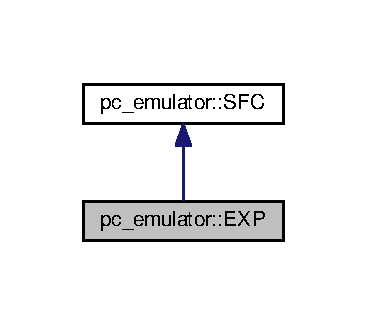
\includegraphics[width=176pt]{classpc__emulator_1_1EXP__inherit__graph}
\end{center}
\end{figure}


Collaboration diagram for pc\+\_\+emulator\+:\+:E\+XP\+:\nopagebreak
\begin{figure}[H]
\begin{center}
\leavevmode
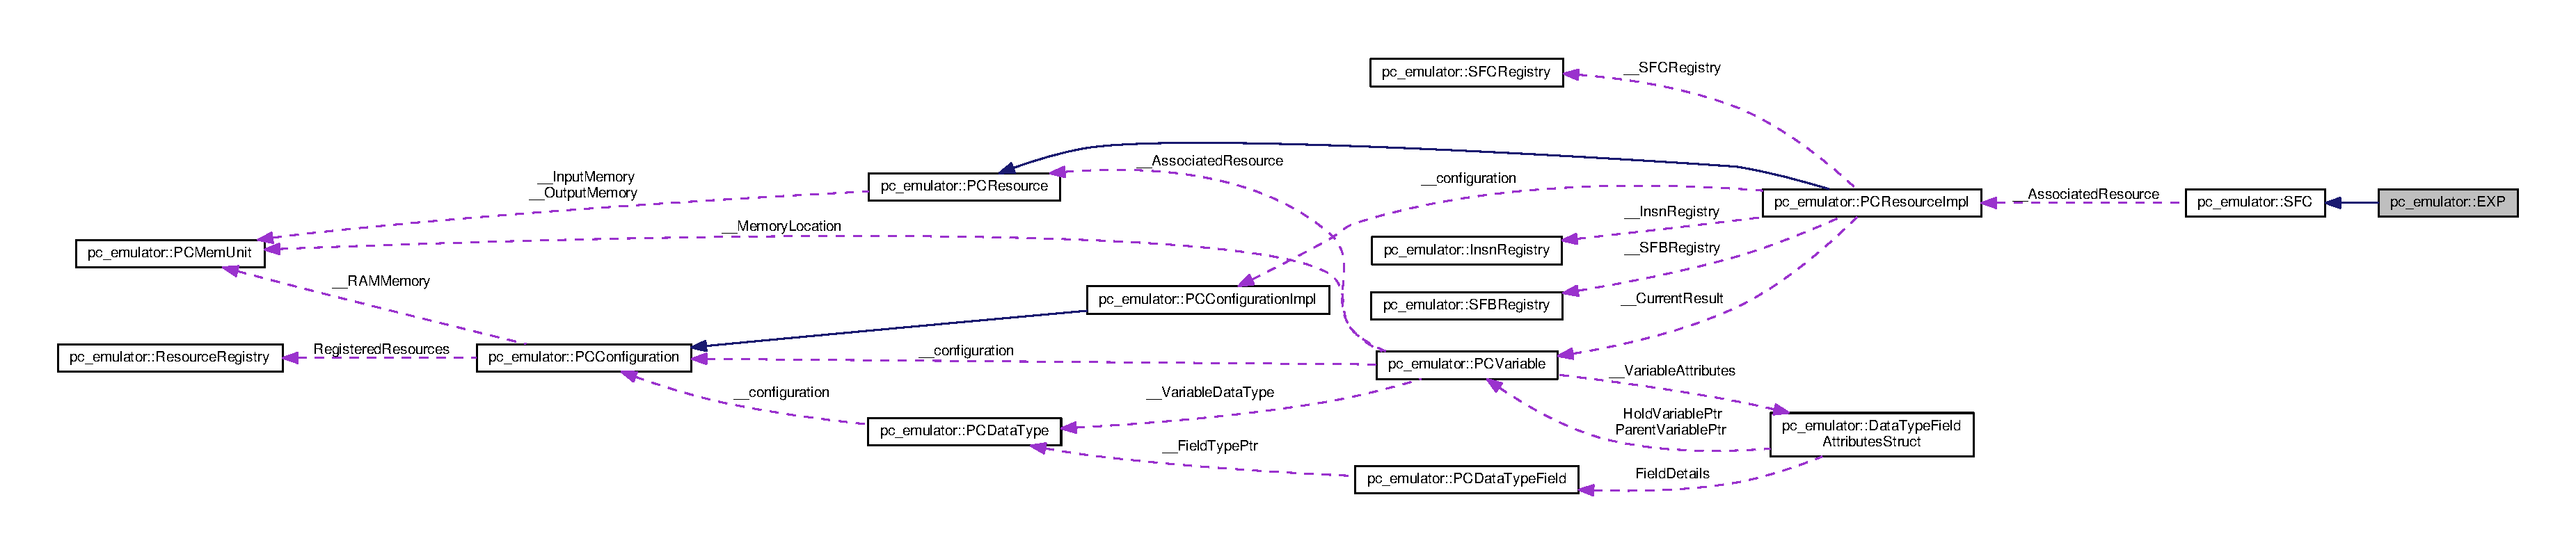
\includegraphics[width=350pt]{classpc__emulator_1_1EXP__coll__graph}
\end{center}
\end{figure}
\subsection*{Public Member Functions}
\begin{DoxyCompactItemize}
\item 
{\bfseries E\+XP} (\hyperlink{classpc__emulator_1_1PCResourceImpl}{P\+C\+Resource\+Impl} $\ast$Associated\+Resource)\hypertarget{classpc__emulator_1_1EXP_ae2f758abc80e38927ffd59f6cadb60c6}{}\label{classpc__emulator_1_1EXP_ae2f758abc80e38927ffd59f6cadb60c6}

\item 
void \hyperlink{classpc__emulator_1_1EXP_aa5a73e7f83ab1b8c692d8a40c634f967}{Execute} (\hyperlink{classpc__emulator_1_1PCVariable}{P\+C\+Variable} $\ast$Current\+Result, std\+::vector$<$ \hyperlink{classpc__emulator_1_1PCVariable}{P\+C\+Variable} $\ast$ $>$ \&Operands)
\begin{DoxyCompactList}\small\item\em Called to execute the sfc. \end{DoxyCompactList}\end{DoxyCompactItemize}
\subsection*{Additional Inherited Members}


\subsection{Detailed Description}
Definition of \hyperlink{classpc__emulator_1_1EXP}{E\+XP} \hyperlink{classpc__emulator_1_1SFC}{S\+FC}. 

\subsection{Member Function Documentation}
\index{pc\+\_\+emulator\+::\+E\+XP@{pc\+\_\+emulator\+::\+E\+XP}!Execute@{Execute}}
\index{Execute@{Execute}!pc\+\_\+emulator\+::\+E\+XP@{pc\+\_\+emulator\+::\+E\+XP}}
\subsubsection[{\texorpdfstring{Execute(\+P\+C\+Variable $\ast$\+Current\+Result, std\+::vector$<$ P\+C\+Variable $\ast$ $>$ \&\+Operands)}{Execute(PCVariable *CurrentResult, std::vector< PCVariable * > &Operands)}}]{\setlength{\rightskip}{0pt plus 5cm}void pc\+\_\+emulator\+::\+E\+X\+P\+::\+Execute (
\begin{DoxyParamCaption}
\item[{{\bf P\+C\+Variable} $\ast$}]{Current\+Result, }
\item[{std\+::vector$<$ {\bf P\+C\+Variable} $\ast$ $>$ \&}]{Operands}
\end{DoxyParamCaption}
)\hspace{0.3cm}{\ttfamily [virtual]}}\hypertarget{classpc__emulator_1_1EXP_aa5a73e7f83ab1b8c692d8a40c634f967}{}\label{classpc__emulator_1_1EXP_aa5a73e7f83ab1b8c692d8a40c634f967}


Called to execute the sfc. 


\begin{DoxyParams}{Parameters}
{\em Current\+Result} & The Current\+Result register of the task executing this \hyperlink{classpc__emulator_1_1SFC}{S\+FC} \\
\hline
{\em Operands} & Operands to the sfc \\
\hline
\end{DoxyParams}


Implements \hyperlink{classpc__emulator_1_1SFC_ab206c80fc0e429c56672b4f6a0ca8635}{pc\+\_\+emulator\+::\+S\+FC}.



The documentation for this class was generated from the following file\+:\begin{DoxyCompactItemize}
\item 
src/pc\+\_\+emulator/include/sfc/exp.\+h\end{DoxyCompactItemize}

\hypertarget{classpc__emulator_1_1ExtModule}{}\section{pc\+\_\+emulator\+:\+:Ext\+Module Class Reference}
\label{classpc__emulator_1_1ExtModule}\index{pc\+\_\+emulator\+::\+Ext\+Module@{pc\+\_\+emulator\+::\+Ext\+Module}}


External module interface.  




{\ttfamily \#include $<$ext\+\_\+module\+\_\+intf.\+h$>$}



Inheritance diagram for pc\+\_\+emulator\+:\+:Ext\+Module\+:
\nopagebreak
\begin{figure}[H]
\begin{center}
\leavevmode
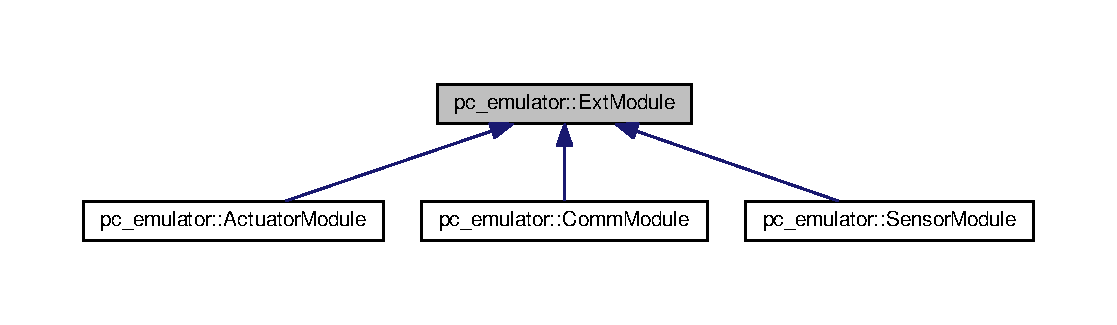
\includegraphics[width=350pt]{classpc__emulator_1_1ExtModule__inherit__graph}
\end{center}
\end{figure}


Collaboration diagram for pc\+\_\+emulator\+:\+:Ext\+Module\+:
\nopagebreak
\begin{figure}[H]
\begin{center}
\leavevmode
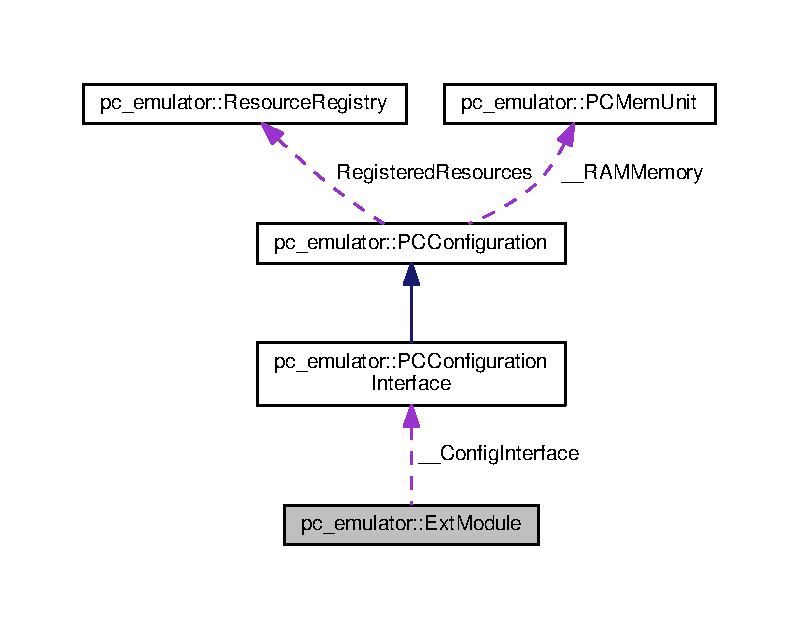
\includegraphics[width=350pt]{classpc__emulator_1_1ExtModule__coll__graph}
\end{center}
\end{figure}
\subsection*{Public Member Functions}
\begin{DoxyCompactItemize}
\item 
\hyperlink{classpc__emulator_1_1ExtModule_a968271fb30effa6ee61d1e790db702bb}{Ext\+Module} (string Configuration\+Path)\hypertarget{classpc__emulator_1_1ExtModule_a968271fb30effa6ee61d1e790db702bb}{}\label{classpc__emulator_1_1ExtModule_a968271fb30effa6ee61d1e790db702bb}

\begin{DoxyCompactList}\small\item\em Constructor. \end{DoxyCompactList}\item 
\hyperlink{classpc__emulator_1_1PCDataType}{P\+C\+Data\+Type} $\ast$ \hyperlink{classpc__emulator_1_1ExtModule_a7ea76b9a1428e26437b7736d558ab918}{Get\+Data\+Type} (string Data\+Type\+Name)
\begin{DoxyCompactList}\small\item\em Returns datatype with the specified name. \end{DoxyCompactList}\item 
virtual std\+::unique\+\_\+ptr$<$ \hyperlink{classpc__emulator_1_1PCVariableContainer}{P\+C\+Variable\+Container} $>$ \hyperlink{classpc__emulator_1_1ExtModule_a5a967d2cf1925ae2f2811892e034db14}{Get\+Variable\+Container} (string Access\+Path)=0
\begin{DoxyCompactList}\small\item\em Should returns a Variable\+Container for the specified access path. \end{DoxyCompactList}\item 
virtual std\+::unique\+\_\+ptr$<$ \hyperlink{classpc__emulator_1_1PCVariableContainer}{P\+C\+Variable\+Container} $>$ \hyperlink{classpc__emulator_1_1ExtModule_a840b25e14892e09ecca10f195cd08e6d}{Get\+Variable\+Container} (int Ram\+Byte\+Offset, int Ram\+Bit\+Offset, string Variable\+Data\+Type\+Name)=0
\begin{DoxyCompactList}\small\item\em Should return a Variable\+Container to the specified R\+AM location. \end{DoxyCompactList}\item 
virtual std\+::unique\+\_\+ptr$<$ \hyperlink{classpc__emulator_1_1PCVariableContainer}{P\+C\+Variable\+Container} $>$ \hyperlink{classpc__emulator_1_1ExtModule_ab62dc4b158134b37e1851a79e009b194}{Get\+Variable\+Container} (string Resource\+Name, int Mem\+Type, int Byte\+Offset, int Bit\+Offset, string Variable\+Data\+Type\+Name)=0
\begin{DoxyCompactList}\small\item\em Should return a Variable\+Container to the specified location. \end{DoxyCompactList}\item 
void \hyperlink{classpc__emulator_1_1ExtModule_aa54675227fb0b02e0f122ab0fa3c0641}{Cleanup} ()\hypertarget{classpc__emulator_1_1ExtModule_aa54675227fb0b02e0f122ab0fa3c0641}{}\label{classpc__emulator_1_1ExtModule_aa54675227fb0b02e0f122ab0fa3c0641}

\begin{DoxyCompactList}\small\item\em Cleans up the configuration interface object. \end{DoxyCompactList}\end{DoxyCompactItemize}
\subsection*{Protected Attributes}
\begin{DoxyCompactItemize}
\item 
\hyperlink{classpc__emulator_1_1PCConfigurationInterface}{P\+C\+Configuration\+Interface} \hyperlink{classpc__emulator_1_1ExtModule_abb29047b24c68d98aa045031f4a12184}{\+\_\+\+\_\+\+Config\+Interface}
\end{DoxyCompactItemize}


\subsection{Detailed Description}
External module interface. 

\subsection{Member Function Documentation}
\index{pc\+\_\+emulator\+::\+Ext\+Module@{pc\+\_\+emulator\+::\+Ext\+Module}!Get\+Data\+Type@{Get\+Data\+Type}}
\index{Get\+Data\+Type@{Get\+Data\+Type}!pc\+\_\+emulator\+::\+Ext\+Module@{pc\+\_\+emulator\+::\+Ext\+Module}}
\subsubsection[{\texorpdfstring{Get\+Data\+Type(string Data\+Type\+Name)}{GetDataType(string DataTypeName)}}]{\setlength{\rightskip}{0pt plus 5cm}{\bf P\+C\+Data\+Type}$\ast$ pc\+\_\+emulator\+::\+Ext\+Module\+::\+Get\+Data\+Type (
\begin{DoxyParamCaption}
\item[{string}]{Data\+Type\+Name}
\end{DoxyParamCaption}
)\hspace{0.3cm}{\ttfamily [inline]}}\hypertarget{classpc__emulator_1_1ExtModule_a7ea76b9a1428e26437b7736d558ab918}{}\label{classpc__emulator_1_1ExtModule_a7ea76b9a1428e26437b7736d558ab918}


Returns datatype with the specified name. 


\begin{DoxyParams}{Parameters}
{\em Data\+Type\+Name} & Name of the data type \\
\hline
\end{DoxyParams}
\begin{DoxyReturn}{Returns}
\hyperlink{classpc__emulator_1_1PCDataType}{P\+C\+Data\+Type} object or nullptr if the data type is not found ! 
\end{DoxyReturn}
\index{pc\+\_\+emulator\+::\+Ext\+Module@{pc\+\_\+emulator\+::\+Ext\+Module}!Get\+Variable\+Container@{Get\+Variable\+Container}}
\index{Get\+Variable\+Container@{Get\+Variable\+Container}!pc\+\_\+emulator\+::\+Ext\+Module@{pc\+\_\+emulator\+::\+Ext\+Module}}
\subsubsection[{\texorpdfstring{Get\+Variable\+Container(string Access\+Path)=0}{GetVariableContainer(string AccessPath)=0}}]{\setlength{\rightskip}{0pt plus 5cm}virtual std\+::unique\+\_\+ptr$<${\bf P\+C\+Variable\+Container}$>$ pc\+\_\+emulator\+::\+Ext\+Module\+::\+Get\+Variable\+Container (
\begin{DoxyParamCaption}
\item[{string}]{Access\+Path}
\end{DoxyParamCaption}
)\hspace{0.3cm}{\ttfamily [pure virtual]}}\hypertarget{classpc__emulator_1_1ExtModule_a5a967d2cf1925ae2f2811892e034db14}{}\label{classpc__emulator_1_1ExtModule_a5a967d2cf1925ae2f2811892e034db14}


Should returns a Variable\+Container for the specified access path. 


\begin{DoxyParams}{Parameters}
{\em Access\+Path} & Access\+Path name (Cannot be a nested field) \\
\hline
\end{DoxyParams}
\begin{DoxyReturn}{Returns}
Variable\+Container or nullptr if Access\+Path is not found! 
\end{DoxyReturn}


Implemented in \hyperlink{classpc__emulator_1_1CommModule_a1643e230094b1ffbcaedcfa1de0f8bc8}{pc\+\_\+emulator\+::\+Comm\+Module}, \hyperlink{classpc__emulator_1_1SensorModule_aa7ed0083532cab1380b6573f96760efa}{pc\+\_\+emulator\+::\+Sensor\+Module}, and \hyperlink{classpc__emulator_1_1ActuatorModule_a3d7f86c890cfd8301bd8481f235457d4}{pc\+\_\+emulator\+::\+Actuator\+Module}.

\index{pc\+\_\+emulator\+::\+Ext\+Module@{pc\+\_\+emulator\+::\+Ext\+Module}!Get\+Variable\+Container@{Get\+Variable\+Container}}
\index{Get\+Variable\+Container@{Get\+Variable\+Container}!pc\+\_\+emulator\+::\+Ext\+Module@{pc\+\_\+emulator\+::\+Ext\+Module}}
\subsubsection[{\texorpdfstring{Get\+Variable\+Container(int Ram\+Byte\+Offset, int Ram\+Bit\+Offset, string Variable\+Data\+Type\+Name)=0}{GetVariableContainer(int RamByteOffset, int RamBitOffset, string VariableDataTypeName)=0}}]{\setlength{\rightskip}{0pt plus 5cm}virtual std\+::unique\+\_\+ptr$<${\bf P\+C\+Variable\+Container}$>$ pc\+\_\+emulator\+::\+Ext\+Module\+::\+Get\+Variable\+Container (
\begin{DoxyParamCaption}
\item[{int}]{Ram\+Byte\+Offset, }
\item[{int}]{Ram\+Bit\+Offset, }
\item[{string}]{Variable\+Data\+Type\+Name}
\end{DoxyParamCaption}
)\hspace{0.3cm}{\ttfamily [pure virtual]}}\hypertarget{classpc__emulator_1_1ExtModule_a840b25e14892e09ecca10f195cd08e6d}{}\label{classpc__emulator_1_1ExtModule_a840b25e14892e09ecca10f195cd08e6d}


Should return a Variable\+Container to the specified R\+AM location. 


\begin{DoxyParams}{Parameters}
{\em Ram\+Byte\+Offset} & Byte of the R\+AM \\
\hline
{\em Ram\+Bit\+Offset} & Bit offset within the byte \\
\hline
{\em Variable\+Data\+Type\+Name} & Initializes the Variable Container to hold a variable of this type \\
\hline
\end{DoxyParams}
\begin{DoxyReturn}{Returns}
A variable container pointing to the specified memory location 
\end{DoxyReturn}


Implemented in \hyperlink{classpc__emulator_1_1CommModule_a674b8ae9e9655c59be67ebd05f66107d}{pc\+\_\+emulator\+::\+Comm\+Module}, \hyperlink{classpc__emulator_1_1SensorModule_affa170aa3378e2a1947eb761b308ad04}{pc\+\_\+emulator\+::\+Sensor\+Module}, and \hyperlink{classpc__emulator_1_1ActuatorModule_a0708323c05eec00925ad87fe95139ce4}{pc\+\_\+emulator\+::\+Actuator\+Module}.

\index{pc\+\_\+emulator\+::\+Ext\+Module@{pc\+\_\+emulator\+::\+Ext\+Module}!Get\+Variable\+Container@{Get\+Variable\+Container}}
\index{Get\+Variable\+Container@{Get\+Variable\+Container}!pc\+\_\+emulator\+::\+Ext\+Module@{pc\+\_\+emulator\+::\+Ext\+Module}}
\subsubsection[{\texorpdfstring{Get\+Variable\+Container(string Resource\+Name, int Mem\+Type, int Byte\+Offset, int Bit\+Offset, string Variable\+Data\+Type\+Name)=0}{GetVariableContainer(string ResourceName, int MemType, int ByteOffset, int BitOffset, string VariableDataTypeName)=0}}]{\setlength{\rightskip}{0pt plus 5cm}virtual std\+::unique\+\_\+ptr$<${\bf P\+C\+Variable\+Container}$>$ pc\+\_\+emulator\+::\+Ext\+Module\+::\+Get\+Variable\+Container (
\begin{DoxyParamCaption}
\item[{string}]{Resource\+Name, }
\item[{int}]{Mem\+Type, }
\item[{int}]{Byte\+Offset, }
\item[{int}]{Bit\+Offset, }
\item[{string}]{Variable\+Data\+Type\+Name}
\end{DoxyParamCaption}
)\hspace{0.3cm}{\ttfamily [pure virtual]}}\hypertarget{classpc__emulator_1_1ExtModule_ab62dc4b158134b37e1851a79e009b194}{}\label{classpc__emulator_1_1ExtModule_ab62dc4b158134b37e1851a79e009b194}


Should return a Variable\+Container to the specified location. 


\begin{DoxyParams}{Parameters}
{\em Resource\+Name} & Name of the resource \\
\hline
{\em Mem\+Type} & I\+N\+P\+UT or O\+U\+T\+P\+UT. If specified as R\+AM, then Resource\+Name is ignored \\
\hline
{\em Byte\+Offset} & Byte of the memory \\
\hline
{\em Bit\+Offset} & Bit offset within the byte \\
\hline
{\em Variable\+Data\+Type\+Name} & Initializes the Variable Container to hold a variable of this type \\
\hline
\end{DoxyParams}
\begin{DoxyReturn}{Returns}
A variable container pointing to the specified memory location 
\end{DoxyReturn}


Implemented in \hyperlink{classpc__emulator_1_1SensorModule_af8b9aaded3c5eafff7742f79bb4b52fd}{pc\+\_\+emulator\+::\+Sensor\+Module}, \hyperlink{classpc__emulator_1_1ActuatorModule_a9a11319d8be1d35f290c3172fe3f5465}{pc\+\_\+emulator\+::\+Actuator\+Module}, and \hyperlink{classpc__emulator_1_1CommModule_af99e6d65047aae685e4292814f85c33b}{pc\+\_\+emulator\+::\+Comm\+Module}.



\subsection{Member Data Documentation}
\index{pc\+\_\+emulator\+::\+Ext\+Module@{pc\+\_\+emulator\+::\+Ext\+Module}!\+\_\+\+\_\+\+Config\+Interface@{\+\_\+\+\_\+\+Config\+Interface}}
\index{\+\_\+\+\_\+\+Config\+Interface@{\+\_\+\+\_\+\+Config\+Interface}!pc\+\_\+emulator\+::\+Ext\+Module@{pc\+\_\+emulator\+::\+Ext\+Module}}
\subsubsection[{\texorpdfstring{\+\_\+\+\_\+\+Config\+Interface}{__ConfigInterface}}]{\setlength{\rightskip}{0pt plus 5cm}{\bf P\+C\+Configuration\+Interface} pc\+\_\+emulator\+::\+Ext\+Module\+::\+\_\+\+\_\+\+Config\+Interface\hspace{0.3cm}{\ttfamily [protected]}}\hypertarget{classpc__emulator_1_1ExtModule_abb29047b24c68d98aa045031f4a12184}{}\label{classpc__emulator_1_1ExtModule_abb29047b24c68d98aa045031f4a12184}
Associated Config Interface 

The documentation for this class was generated from the following file\+:\begin{DoxyCompactItemize}
\item 
src/pc\+\_\+emulator/ext\+\_\+modules/include/ext\+\_\+module\+\_\+intf.\+h\end{DoxyCompactItemize}

\hypertarget{classpc__emulator_1_1FunctionsRegistry}{}\section{pc\+\_\+emulator\+:\+:Functions\+Registry Class Reference}
\label{classpc__emulator_1_1FunctionsRegistry}\index{pc\+\_\+emulator\+::\+Functions\+Registry@{pc\+\_\+emulator\+::\+Functions\+Registry}}


Class which registers and tracks all valid Functions with a Code Body.  




{\ttfamily \#include $<$functions\+\_\+registry.\+h$>$}

\subsection*{Public Member Functions}
\begin{DoxyCompactItemize}
\item 
\hyperlink{classpc__emulator_1_1FunctionsRegistry_a2f91b245b966f4fd6231817829d08ae7}{Functions\+Registry} (\hyperlink{classpc__emulator_1_1PCResourceImpl}{P\+C\+Resource\+Impl} $\ast$Associated\+Resource)\hypertarget{classpc__emulator_1_1FunctionsRegistry_a2f91b245b966f4fd6231817829d08ae7}{}\label{classpc__emulator_1_1FunctionsRegistry_a2f91b245b966f4fd6231817829d08ae7}

\begin{DoxyCompactList}\small\item\em Constructor. \end{DoxyCompactList}\item 
\hyperlink{classpc__emulator_1_1PCVariable}{P\+C\+Variable} $\ast$ \hyperlink{classpc__emulator_1_1FunctionsRegistry_a846c3466af0ab96c5089e9b09c608799}{Get\+Function} (string Fn\+Name)
\begin{DoxyCompactList}\small\item\em Retrieve Function variable object with the specified name. \end{DoxyCompactList}\end{DoxyCompactItemize}


\subsection{Detailed Description}
Class which registers and tracks all valid Functions with a Code Body. 

\subsection{Member Function Documentation}
\index{pc\+\_\+emulator\+::\+Functions\+Registry@{pc\+\_\+emulator\+::\+Functions\+Registry}!Get\+Function@{Get\+Function}}
\index{Get\+Function@{Get\+Function}!pc\+\_\+emulator\+::\+Functions\+Registry@{pc\+\_\+emulator\+::\+Functions\+Registry}}
\subsubsection[{\texorpdfstring{Get\+Function(string Fn\+Name)}{GetFunction(string FnName)}}]{\setlength{\rightskip}{0pt plus 5cm}{\bf P\+C\+Variable}$\ast$ pc\+\_\+emulator\+::\+Functions\+Registry\+::\+Get\+Function (
\begin{DoxyParamCaption}
\item[{string}]{Fn\+Name}
\end{DoxyParamCaption}
)}\hypertarget{classpc__emulator_1_1FunctionsRegistry_a846c3466af0ab96c5089e9b09c608799}{}\label{classpc__emulator_1_1FunctionsRegistry_a846c3466af0ab96c5089e9b09c608799}


Retrieve Function variable object with the specified name. 


\begin{DoxyParams}{Parameters}
{\em Fn\+Name} & Name of the Function \\
\hline
\end{DoxyParams}
\begin{DoxyReturn}{Returns}
Function variable object 
\end{DoxyReturn}


The documentation for this class was generated from the following file\+:\begin{DoxyCompactItemize}
\item 
src/pc\+\_\+emulator/include/functions\+\_\+registry.\+h\end{DoxyCompactItemize}

\hypertarget{classpc__emulator_1_1GE__Insn}{}\section{pc\+\_\+emulator\+:\+:G\+E\+\_\+\+Insn Class Reference}
\label{classpc__emulator_1_1GE__Insn}\index{pc\+\_\+emulator\+::\+G\+E\+\_\+\+Insn@{pc\+\_\+emulator\+::\+G\+E\+\_\+\+Insn}}


Greater than or equal instruction.  




{\ttfamily \#include $<$ge\+\_\+insn.\+h$>$}



Inheritance diagram for pc\+\_\+emulator\+:\+:G\+E\+\_\+\+Insn\+:\nopagebreak
\begin{figure}[H]
\begin{center}
\leavevmode
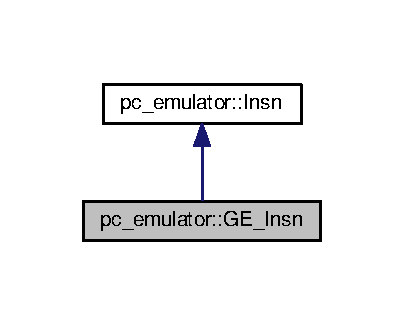
\includegraphics[width=194pt]{classpc__emulator_1_1GE__Insn__inherit__graph}
\end{center}
\end{figure}


Collaboration diagram for pc\+\_\+emulator\+:\+:G\+E\+\_\+\+Insn\+:\nopagebreak
\begin{figure}[H]
\begin{center}
\leavevmode
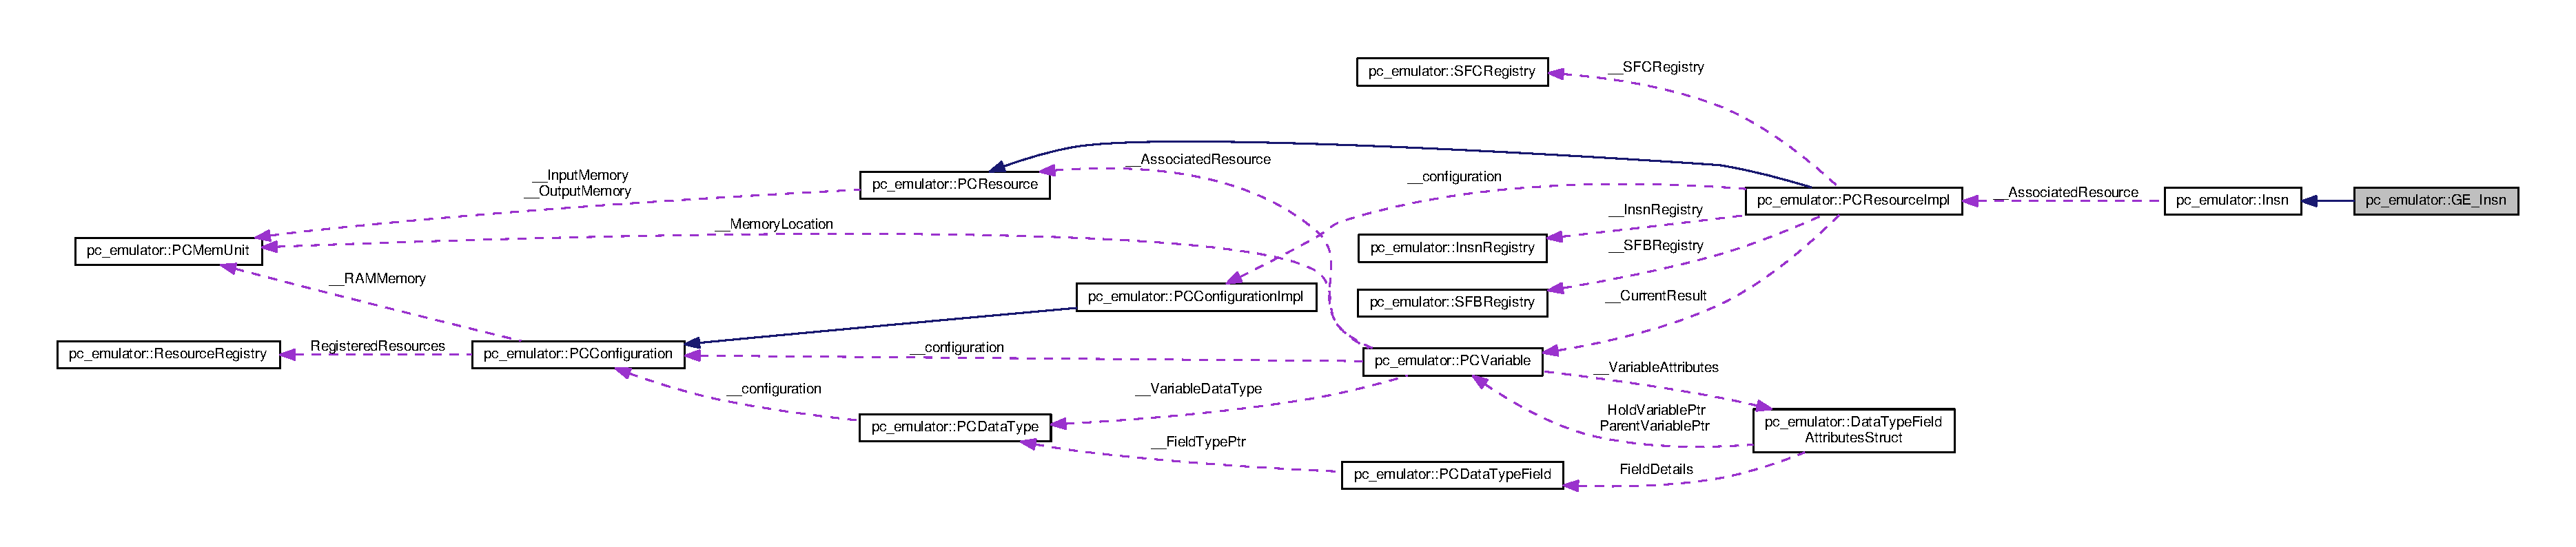
\includegraphics[width=350pt]{classpc__emulator_1_1GE__Insn__coll__graph}
\end{center}
\end{figure}
\subsection*{Public Member Functions}
\begin{DoxyCompactItemize}
\item 
{\bfseries G\+E\+\_\+\+Insn} (\hyperlink{classpc__emulator_1_1PCResourceImpl}{P\+C\+Resource\+Impl} $\ast$Associated\+Resource, bool is\+Negated)\hypertarget{classpc__emulator_1_1GE__Insn_a4e69a7b11f031ac0f976d228136f3447}{}\label{classpc__emulator_1_1GE__Insn_a4e69a7b11f031ac0f976d228136f3447}

\item 
void \hyperlink{classpc__emulator_1_1GE__Insn_adad83e1724742a0c9ea77516bb85c22b}{Execute} (\hyperlink{classpc__emulator_1_1PCVariable}{P\+C\+Variable} $\ast$Current\+Result, std\+::vector$<$ \hyperlink{classpc__emulator_1_1PCVariable}{P\+C\+Variable} $\ast$ $>$ \&Operands)
\begin{DoxyCompactList}\small\item\em Called to execute the instruction. \end{DoxyCompactList}\end{DoxyCompactItemize}
\subsection*{Additional Inherited Members}


\subsection{Detailed Description}
Greater than or equal instruction. 

\subsection{Member Function Documentation}
\index{pc\+\_\+emulator\+::\+G\+E\+\_\+\+Insn@{pc\+\_\+emulator\+::\+G\+E\+\_\+\+Insn}!Execute@{Execute}}
\index{Execute@{Execute}!pc\+\_\+emulator\+::\+G\+E\+\_\+\+Insn@{pc\+\_\+emulator\+::\+G\+E\+\_\+\+Insn}}
\subsubsection[{\texorpdfstring{Execute(\+P\+C\+Variable $\ast$\+Current\+Result, std\+::vector$<$ P\+C\+Variable $\ast$ $>$ \&\+Operands)}{Execute(PCVariable *CurrentResult, std::vector< PCVariable * > &Operands)}}]{\setlength{\rightskip}{0pt plus 5cm}void pc\+\_\+emulator\+::\+G\+E\+\_\+\+Insn\+::\+Execute (
\begin{DoxyParamCaption}
\item[{{\bf P\+C\+Variable} $\ast$}]{Current\+Result, }
\item[{std\+::vector$<$ {\bf P\+C\+Variable} $\ast$ $>$ \&}]{Operands}
\end{DoxyParamCaption}
)\hspace{0.3cm}{\ttfamily [virtual]}}\hypertarget{classpc__emulator_1_1GE__Insn_adad83e1724742a0c9ea77516bb85c22b}{}\label{classpc__emulator_1_1GE__Insn_adad83e1724742a0c9ea77516bb85c22b}


Called to execute the instruction. 


\begin{DoxyParams}{Parameters}
{\em Current\+Result} & The Current\+Result register of the task executing this \hyperlink{classpc__emulator_1_1Insn}{Insn} \\
\hline
{\em Operands} & Operands to the instruction \\
\hline
\end{DoxyParams}


Implements \hyperlink{classpc__emulator_1_1Insn_a103d27030e872a799e313df16c1f3d66}{pc\+\_\+emulator\+::\+Insn}.



The documentation for this class was generated from the following file\+:\begin{DoxyCompactItemize}
\item 
src/pc\+\_\+emulator/include/insns/ge\+\_\+insn.\+h\end{DoxyCompactItemize}

\hypertarget{classpc__emulator_1_1GT__Insn}{}\section{pc\+\_\+emulator\+:\+:G\+T\+\_\+\+Insn Class Reference}
\label{classpc__emulator_1_1GT__Insn}\index{pc\+\_\+emulator\+::\+G\+T\+\_\+\+Insn@{pc\+\_\+emulator\+::\+G\+T\+\_\+\+Insn}}


Greater than instruction.  




{\ttfamily \#include $<$gt\+\_\+insn.\+h$>$}



Inheritance diagram for pc\+\_\+emulator\+:\+:G\+T\+\_\+\+Insn\+:
\nopagebreak
\begin{figure}[H]
\begin{center}
\leavevmode
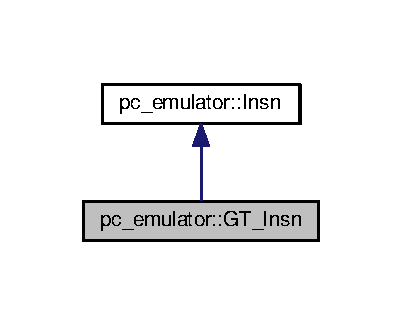
\includegraphics[width=193pt]{classpc__emulator_1_1GT__Insn__inherit__graph}
\end{center}
\end{figure}


Collaboration diagram for pc\+\_\+emulator\+:\+:G\+T\+\_\+\+Insn\+:
\nopagebreak
\begin{figure}[H]
\begin{center}
\leavevmode
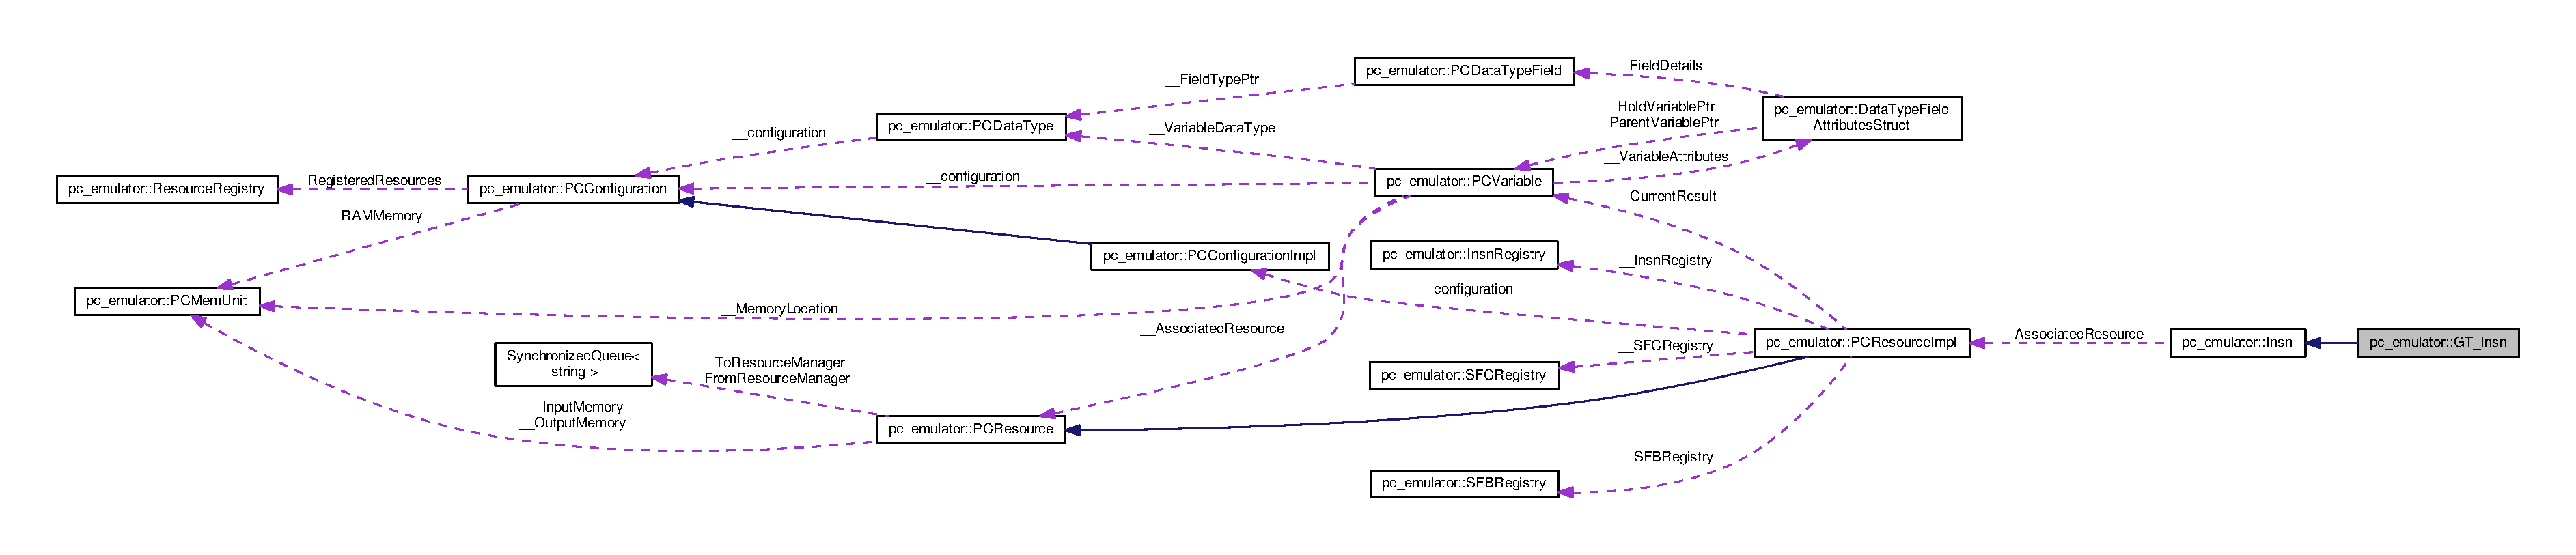
\includegraphics[width=350pt]{classpc__emulator_1_1GT__Insn__coll__graph}
\end{center}
\end{figure}
\subsection*{Public Member Functions}
\begin{DoxyCompactItemize}
\item 
{\bfseries G\+T\+\_\+\+Insn} (\hyperlink{classpc__emulator_1_1PCResourceImpl}{P\+C\+Resource\+Impl} $\ast$Associated\+Resource, bool is\+Negated)\hypertarget{classpc__emulator_1_1GT__Insn_a44d589c4e159bda6d07d236cc62fb03b}{}\label{classpc__emulator_1_1GT__Insn_a44d589c4e159bda6d07d236cc62fb03b}

\item 
void \hyperlink{classpc__emulator_1_1GT__Insn_a90e85b8626651fbbf4a1f5e3522ea7cf}{Execute} (\hyperlink{classpc__emulator_1_1PCVariable}{P\+C\+Variable} $\ast$Current\+Result, std\+::vector$<$ \hyperlink{classpc__emulator_1_1PCVariable}{P\+C\+Variable} $\ast$ $>$ \&Operands)
\begin{DoxyCompactList}\small\item\em Called to execute the instruction. \end{DoxyCompactList}\end{DoxyCompactItemize}
\subsection*{Additional Inherited Members}


\subsection{Detailed Description}
Greater than instruction. 

\subsection{Member Function Documentation}
\index{pc\+\_\+emulator\+::\+G\+T\+\_\+\+Insn@{pc\+\_\+emulator\+::\+G\+T\+\_\+\+Insn}!Execute@{Execute}}
\index{Execute@{Execute}!pc\+\_\+emulator\+::\+G\+T\+\_\+\+Insn@{pc\+\_\+emulator\+::\+G\+T\+\_\+\+Insn}}
\subsubsection[{\texorpdfstring{Execute(\+P\+C\+Variable $\ast$\+Current\+Result, std\+::vector$<$ P\+C\+Variable $\ast$ $>$ \&\+Operands)}{Execute(PCVariable *CurrentResult, std::vector< PCVariable * > &Operands)}}]{\setlength{\rightskip}{0pt plus 5cm}void pc\+\_\+emulator\+::\+G\+T\+\_\+\+Insn\+::\+Execute (
\begin{DoxyParamCaption}
\item[{{\bf P\+C\+Variable} $\ast$}]{Current\+Result, }
\item[{std\+::vector$<$ {\bf P\+C\+Variable} $\ast$ $>$ \&}]{Operands}
\end{DoxyParamCaption}
)\hspace{0.3cm}{\ttfamily [virtual]}}\hypertarget{classpc__emulator_1_1GT__Insn_a90e85b8626651fbbf4a1f5e3522ea7cf}{}\label{classpc__emulator_1_1GT__Insn_a90e85b8626651fbbf4a1f5e3522ea7cf}


Called to execute the instruction. 


\begin{DoxyParams}{Parameters}
{\em Current\+Result} & The Current\+Result register of the task executing this \hyperlink{classpc__emulator_1_1Insn}{Insn} \\
\hline
{\em Operands} & Operands to the instruction \\
\hline
\end{DoxyParams}


Implements \hyperlink{classpc__emulator_1_1Insn_a103d27030e872a799e313df16c1f3d66}{pc\+\_\+emulator\+::\+Insn}.



The documentation for this class was generated from the following file\+:\begin{DoxyCompactItemize}
\item 
src/pc\+\_\+emulator/include/insns/gt\+\_\+insn.\+h\end{DoxyCompactItemize}

\hypertarget{classpc__emulator_1_1GTOD}{}\section{pc\+\_\+emulator\+:\+:G\+T\+OD Class Reference}
\label{classpc__emulator_1_1GTOD}\index{pc\+\_\+emulator\+::\+G\+T\+OD@{pc\+\_\+emulator\+::\+G\+T\+OD}}


Definition of Get Time of Day \hyperlink{classpc__emulator_1_1SFC}{S\+FC}.  




{\ttfamily \#include $<$gtod.\+h$>$}



Inheritance diagram for pc\+\_\+emulator\+:\+:G\+T\+OD\+:\nopagebreak
\begin{figure}[H]
\begin{center}
\leavevmode
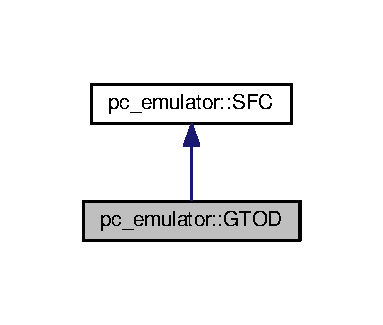
\includegraphics[width=184pt]{classpc__emulator_1_1GTOD__inherit__graph}
\end{center}
\end{figure}


Collaboration diagram for pc\+\_\+emulator\+:\+:G\+T\+OD\+:\nopagebreak
\begin{figure}[H]
\begin{center}
\leavevmode
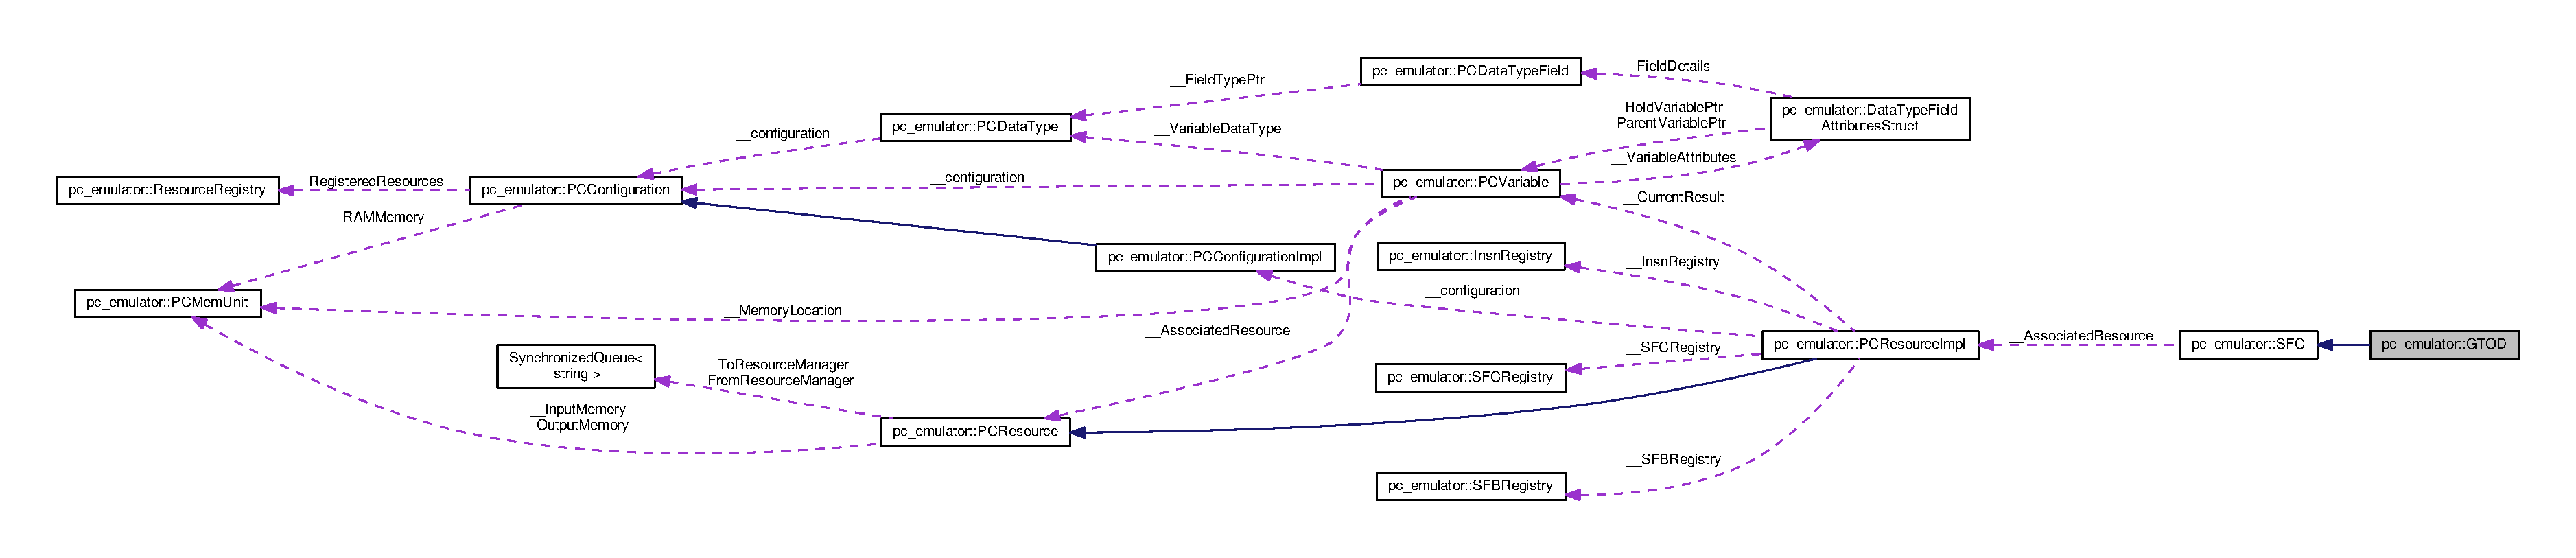
\includegraphics[width=350pt]{classpc__emulator_1_1GTOD__coll__graph}
\end{center}
\end{figure}
\subsection*{Public Member Functions}
\begin{DoxyCompactItemize}
\item 
{\bfseries G\+T\+OD} (\hyperlink{classpc__emulator_1_1PCResourceImpl}{P\+C\+Resource\+Impl} $\ast$Associated\+Resource)\hypertarget{classpc__emulator_1_1GTOD_aaa26827adf081c660bb97409619af5dc}{}\label{classpc__emulator_1_1GTOD_aaa26827adf081c660bb97409619af5dc}

\item 
void \hyperlink{classpc__emulator_1_1GTOD_af8ca5fbbb07e38766d17e817fd2934e4}{Execute} (\hyperlink{classpc__emulator_1_1PCVariable}{P\+C\+Variable} $\ast$Current\+Result, std\+::vector$<$ \hyperlink{classpc__emulator_1_1PCVariable}{P\+C\+Variable} $\ast$ $>$ \&Operands)
\begin{DoxyCompactList}\small\item\em Called to execute the sfc. \end{DoxyCompactList}\end{DoxyCompactItemize}
\subsection*{Additional Inherited Members}


\subsection{Detailed Description}
Definition of Get Time of Day \hyperlink{classpc__emulator_1_1SFC}{S\+FC}. 

\subsection{Member Function Documentation}
\index{pc\+\_\+emulator\+::\+G\+T\+OD@{pc\+\_\+emulator\+::\+G\+T\+OD}!Execute@{Execute}}
\index{Execute@{Execute}!pc\+\_\+emulator\+::\+G\+T\+OD@{pc\+\_\+emulator\+::\+G\+T\+OD}}
\subsubsection[{\texorpdfstring{Execute(\+P\+C\+Variable $\ast$\+Current\+Result, std\+::vector$<$ P\+C\+Variable $\ast$ $>$ \&\+Operands)}{Execute(PCVariable *CurrentResult, std::vector< PCVariable * > &Operands)}}]{\setlength{\rightskip}{0pt plus 5cm}void pc\+\_\+emulator\+::\+G\+T\+O\+D\+::\+Execute (
\begin{DoxyParamCaption}
\item[{{\bf P\+C\+Variable} $\ast$}]{Current\+Result, }
\item[{std\+::vector$<$ {\bf P\+C\+Variable} $\ast$ $>$ \&}]{Operands}
\end{DoxyParamCaption}
)\hspace{0.3cm}{\ttfamily [virtual]}}\hypertarget{classpc__emulator_1_1GTOD_af8ca5fbbb07e38766d17e817fd2934e4}{}\label{classpc__emulator_1_1GTOD_af8ca5fbbb07e38766d17e817fd2934e4}


Called to execute the sfc. 


\begin{DoxyParams}{Parameters}
{\em Current\+Result} & The Current\+Result register of the task executing this \hyperlink{classpc__emulator_1_1SFC}{S\+FC} \\
\hline
{\em Operands} & Operands to the sfc \\
\hline
\end{DoxyParams}


Implements \hyperlink{classpc__emulator_1_1SFC_ab206c80fc0e429c56672b4f6a0ca8635}{pc\+\_\+emulator\+::\+S\+FC}.



The documentation for this class was generated from the following file\+:\begin{DoxyCompactItemize}
\item 
src/pc\+\_\+emulator/include/sfc/gtod.\+h\end{DoxyCompactItemize}

\hypertarget{classpc__emulator_1_1Insn}{}\section{pc\+\_\+emulator\+:\+:Insn Class Reference}
\label{classpc__emulator_1_1Insn}\index{pc\+\_\+emulator\+::\+Insn@{pc\+\_\+emulator\+::\+Insn}}


Generic abstract class for an IL instruction.  




{\ttfamily \#include $<$insn.\+h$>$}



Inheritance diagram for pc\+\_\+emulator\+:\+:Insn\+:\nopagebreak
\begin{figure}[H]
\begin{center}
\leavevmode
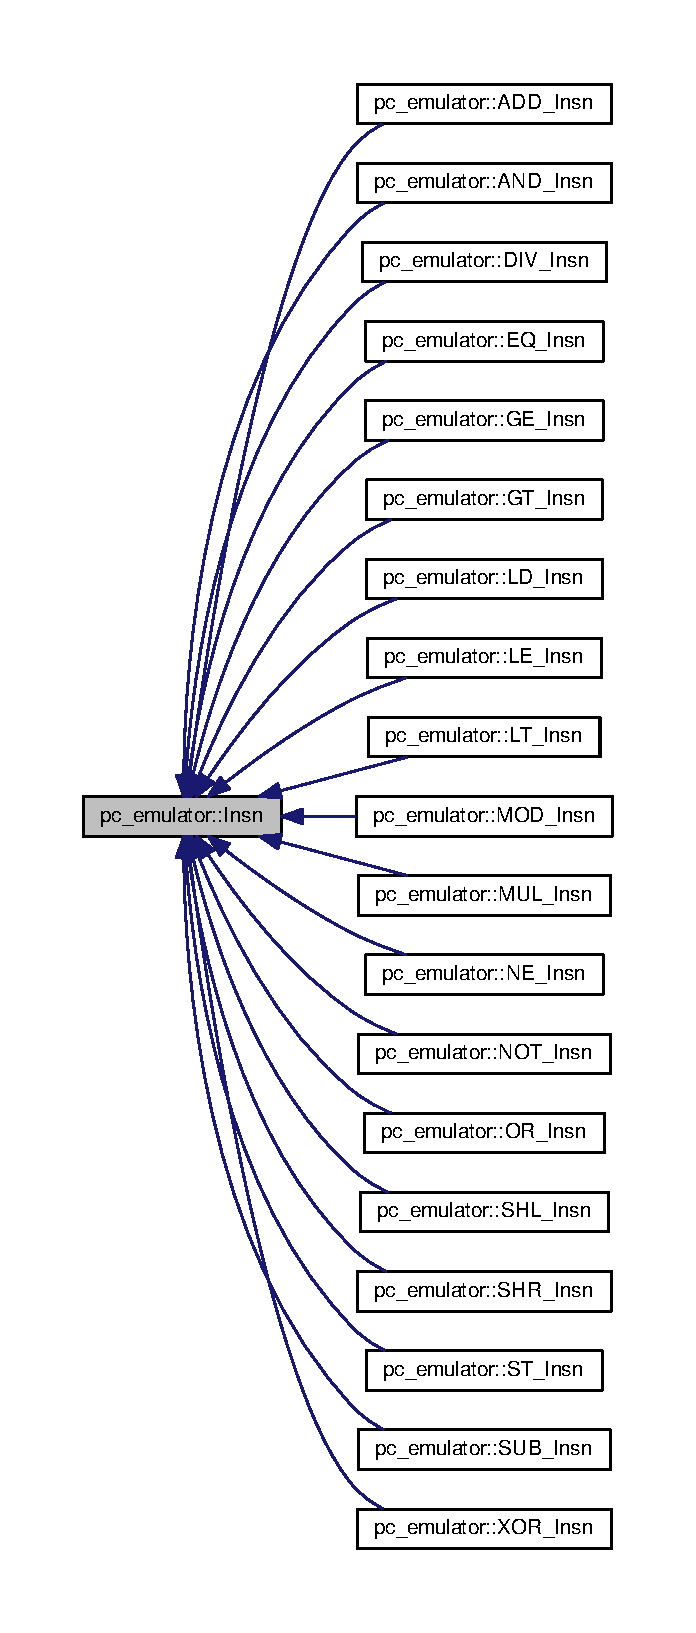
\includegraphics[height=550pt]{classpc__emulator_1_1Insn__inherit__graph}
\end{center}
\end{figure}


Collaboration diagram for pc\+\_\+emulator\+:\+:Insn\+:\nopagebreak
\begin{figure}[H]
\begin{center}
\leavevmode
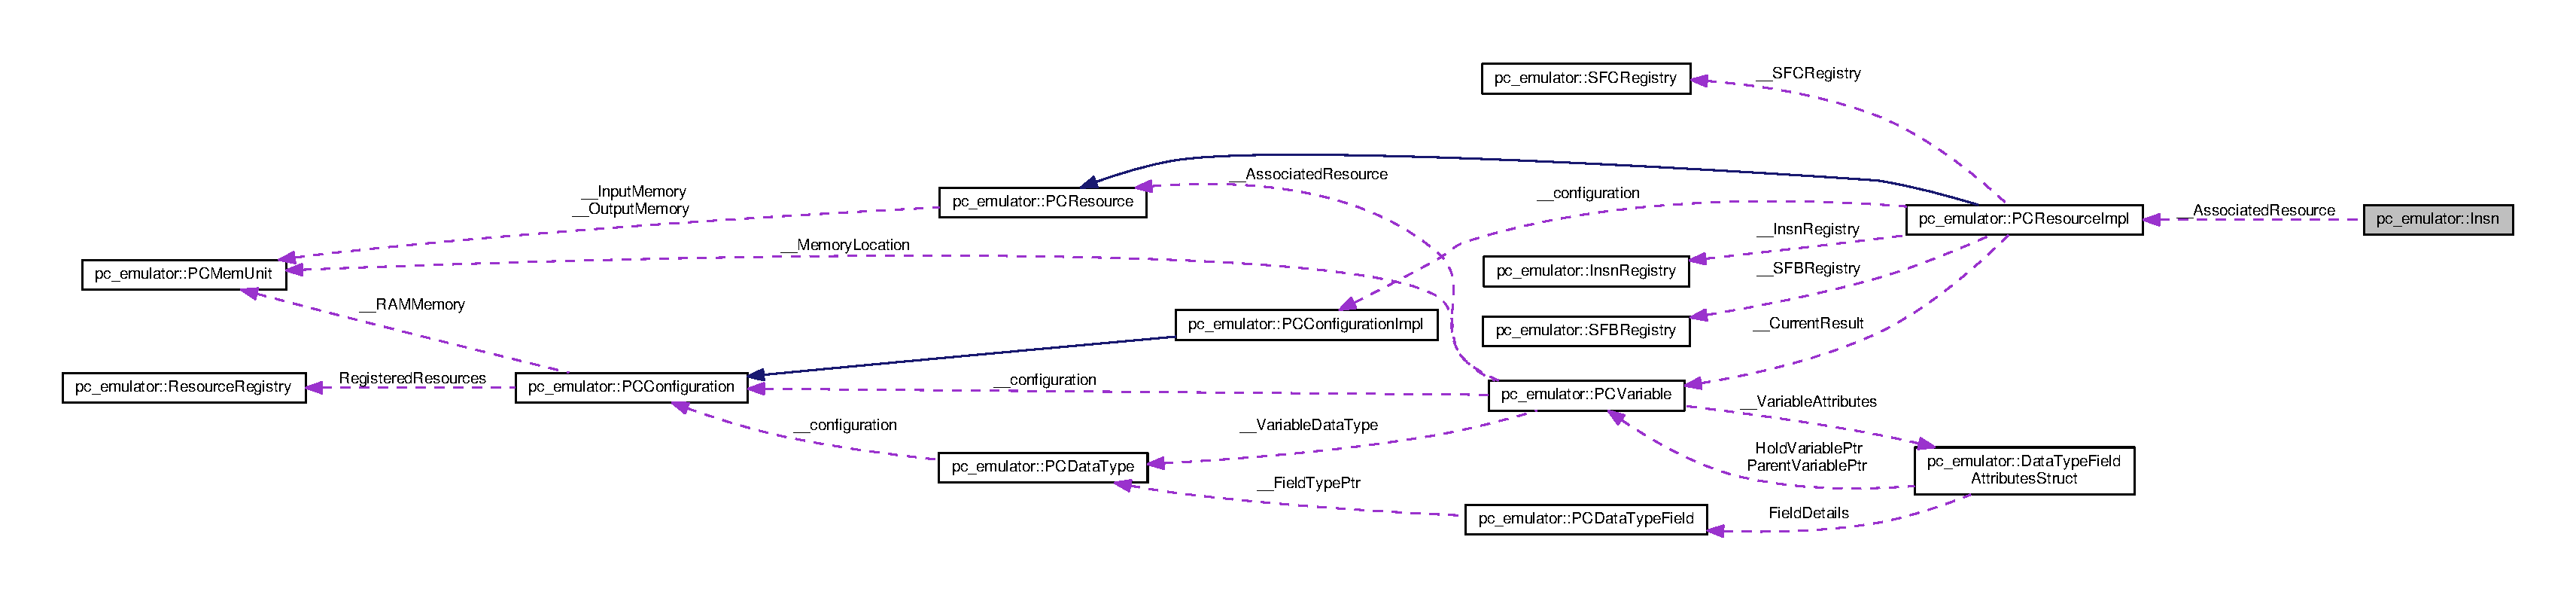
\includegraphics[width=350pt]{classpc__emulator_1_1Insn__coll__graph}
\end{center}
\end{figure}
\subsection*{Public Member Functions}
\begin{DoxyCompactItemize}
\item 
virtual void \hyperlink{classpc__emulator_1_1Insn_a103d27030e872a799e313df16c1f3d66}{Execute} (\hyperlink{classpc__emulator_1_1PCVariable}{P\+C\+Variable} $\ast$Current\+Result, std\+::vector$<$ \hyperlink{classpc__emulator_1_1PCVariable}{P\+C\+Variable} $\ast$ $>$ \&Operands)=0
\begin{DoxyCompactList}\small\item\em Called to execute the instruction. \end{DoxyCompactList}\end{DoxyCompactItemize}
\subsection*{Public Attributes}
\begin{DoxyCompactItemize}
\item 
\hyperlink{classpc__emulator_1_1PCResourceImpl}{P\+C\+Resource\+Impl} $\ast$ \hyperlink{classpc__emulator_1_1Insn_ae7cb9ec6f9eff913027042ad4e253bd4}{\+\_\+\+\_\+\+Associated\+Resource}
\item 
string \hyperlink{classpc__emulator_1_1Insn_a7921073748a0e77469b19bad52b0518b}{\+\_\+\+\_\+\+Insn\+Name}
\item 
bool \hyperlink{classpc__emulator_1_1Insn_a41aa1d28ef8bcf15ca05faaa1ccea018}{Is\+Negated}
\end{DoxyCompactItemize}


\subsection{Detailed Description}
Generic abstract class for an IL instruction. 

\subsection{Member Function Documentation}
\index{pc\+\_\+emulator\+::\+Insn@{pc\+\_\+emulator\+::\+Insn}!Execute@{Execute}}
\index{Execute@{Execute}!pc\+\_\+emulator\+::\+Insn@{pc\+\_\+emulator\+::\+Insn}}
\subsubsection[{\texorpdfstring{Execute(\+P\+C\+Variable $\ast$\+Current\+Result, std\+::vector$<$ P\+C\+Variable $\ast$ $>$ \&\+Operands)=0}{Execute(PCVariable *CurrentResult, std::vector< PCVariable * > &Operands)=0}}]{\setlength{\rightskip}{0pt plus 5cm}virtual void pc\+\_\+emulator\+::\+Insn\+::\+Execute (
\begin{DoxyParamCaption}
\item[{{\bf P\+C\+Variable} $\ast$}]{Current\+Result, }
\item[{std\+::vector$<$ {\bf P\+C\+Variable} $\ast$ $>$ \&}]{Operands}
\end{DoxyParamCaption}
)\hspace{0.3cm}{\ttfamily [pure virtual]}}\hypertarget{classpc__emulator_1_1Insn_a103d27030e872a799e313df16c1f3d66}{}\label{classpc__emulator_1_1Insn_a103d27030e872a799e313df16c1f3d66}


Called to execute the instruction. 


\begin{DoxyParams}{Parameters}
{\em Current\+Result} & The Current\+Result register of the task executing this \hyperlink{classpc__emulator_1_1Insn}{Insn} \\
\hline
{\em Operands} & Operands to the instruction \\
\hline
\end{DoxyParams}


Implemented in \hyperlink{classpc__emulator_1_1SHL__Insn_add61e1603cb45626bf2ca76fa007ad6c}{pc\+\_\+emulator\+::\+S\+H\+L\+\_\+\+Insn}, \hyperlink{classpc__emulator_1_1SHR__Insn_a07645761faeda0b6208da505f2b4f0a8}{pc\+\_\+emulator\+::\+S\+H\+R\+\_\+\+Insn}, \hyperlink{classpc__emulator_1_1ADD__Insn_aebbf49265a5cc15c5ebf6d11ca4ec7c2}{pc\+\_\+emulator\+::\+A\+D\+D\+\_\+\+Insn}, \hyperlink{classpc__emulator_1_1AND__Insn_a97a9a9d54d0d91b435ce763396ec21d9}{pc\+\_\+emulator\+::\+A\+N\+D\+\_\+\+Insn}, \hyperlink{classpc__emulator_1_1DIV__Insn_a25e0da13e7b4ea49277ba62854382c8d}{pc\+\_\+emulator\+::\+D\+I\+V\+\_\+\+Insn}, \hyperlink{classpc__emulator_1_1EQ__Insn_ac0337e98a5bef35cf38880caa03969ed}{pc\+\_\+emulator\+::\+E\+Q\+\_\+\+Insn}, \hyperlink{classpc__emulator_1_1GE__Insn_adad83e1724742a0c9ea77516bb85c22b}{pc\+\_\+emulator\+::\+G\+E\+\_\+\+Insn}, \hyperlink{classpc__emulator_1_1GT__Insn_a90e85b8626651fbbf4a1f5e3522ea7cf}{pc\+\_\+emulator\+::\+G\+T\+\_\+\+Insn}, \hyperlink{classpc__emulator_1_1LE__Insn_a338cea25547481dd6ee9a62569f9bbaf}{pc\+\_\+emulator\+::\+L\+E\+\_\+\+Insn}, \hyperlink{classpc__emulator_1_1LT__Insn_a26d1613e7b8e042f10124d9e6758ff10}{pc\+\_\+emulator\+::\+L\+T\+\_\+\+Insn}, \hyperlink{classpc__emulator_1_1MOD__Insn_ad6555ef4921d88fa8ef48c37c602b0fd}{pc\+\_\+emulator\+::\+M\+O\+D\+\_\+\+Insn}, \hyperlink{classpc__emulator_1_1MUL__Insn_a8575326e90b1bbdf1587a79ba575b733}{pc\+\_\+emulator\+::\+M\+U\+L\+\_\+\+Insn}, \hyperlink{classpc__emulator_1_1NE__Insn_abd2edddfbc2fecbcde5e154293c40ebc}{pc\+\_\+emulator\+::\+N\+E\+\_\+\+Insn}, \hyperlink{classpc__emulator_1_1NOT__Insn_a26832f4fb932e0162f2d80ccdbbd5983}{pc\+\_\+emulator\+::\+N\+O\+T\+\_\+\+Insn}, \hyperlink{classpc__emulator_1_1OR__Insn_a456e9748cd686693f59c7ac53c4c6191}{pc\+\_\+emulator\+::\+O\+R\+\_\+\+Insn}, \hyperlink{classpc__emulator_1_1ST__Insn_aa5d05843972a435e372007f037e1f335}{pc\+\_\+emulator\+::\+S\+T\+\_\+\+Insn}, \hyperlink{classpc__emulator_1_1SUB__Insn_a228667f8f6b794362ce89d8d0c8b2a9a}{pc\+\_\+emulator\+::\+S\+U\+B\+\_\+\+Insn}, \hyperlink{classpc__emulator_1_1XOR__Insn_ac40be2bc902b2a4e10253c9eb1bcd185}{pc\+\_\+emulator\+::\+X\+O\+R\+\_\+\+Insn}, and \hyperlink{classpc__emulator_1_1LD__Insn_a3afc230f457185fefc9f2297d8ab5c29}{pc\+\_\+emulator\+::\+L\+D\+\_\+\+Insn}.



\subsection{Member Data Documentation}
\index{pc\+\_\+emulator\+::\+Insn@{pc\+\_\+emulator\+::\+Insn}!\+\_\+\+\_\+\+Associated\+Resource@{\+\_\+\+\_\+\+Associated\+Resource}}
\index{\+\_\+\+\_\+\+Associated\+Resource@{\+\_\+\+\_\+\+Associated\+Resource}!pc\+\_\+emulator\+::\+Insn@{pc\+\_\+emulator\+::\+Insn}}
\subsubsection[{\texorpdfstring{\+\_\+\+\_\+\+Associated\+Resource}{__AssociatedResource}}]{\setlength{\rightskip}{0pt plus 5cm}{\bf P\+C\+Resource\+Impl}$\ast$ pc\+\_\+emulator\+::\+Insn\+::\+\_\+\+\_\+\+Associated\+Resource}\hypertarget{classpc__emulator_1_1Insn_ae7cb9ec6f9eff913027042ad4e253bd4}{}\label{classpc__emulator_1_1Insn_ae7cb9ec6f9eff913027042ad4e253bd4}
Associated resource \index{pc\+\_\+emulator\+::\+Insn@{pc\+\_\+emulator\+::\+Insn}!\+\_\+\+\_\+\+Insn\+Name@{\+\_\+\+\_\+\+Insn\+Name}}
\index{\+\_\+\+\_\+\+Insn\+Name@{\+\_\+\+\_\+\+Insn\+Name}!pc\+\_\+emulator\+::\+Insn@{pc\+\_\+emulator\+::\+Insn}}
\subsubsection[{\texorpdfstring{\+\_\+\+\_\+\+Insn\+Name}{__InsnName}}]{\setlength{\rightskip}{0pt plus 5cm}string pc\+\_\+emulator\+::\+Insn\+::\+\_\+\+\_\+\+Insn\+Name}\hypertarget{classpc__emulator_1_1Insn_a7921073748a0e77469b19bad52b0518b}{}\label{classpc__emulator_1_1Insn_a7921073748a0e77469b19bad52b0518b}
Instruction name \index{pc\+\_\+emulator\+::\+Insn@{pc\+\_\+emulator\+::\+Insn}!Is\+Negated@{Is\+Negated}}
\index{Is\+Negated@{Is\+Negated}!pc\+\_\+emulator\+::\+Insn@{pc\+\_\+emulator\+::\+Insn}}
\subsubsection[{\texorpdfstring{Is\+Negated}{IsNegated}}]{\setlength{\rightskip}{0pt plus 5cm}bool pc\+\_\+emulator\+::\+Insn\+::\+Is\+Negated}\hypertarget{classpc__emulator_1_1Insn_a41aa1d28ef8bcf15ca05faaa1ccea018}{}\label{classpc__emulator_1_1Insn_a41aa1d28ef8bcf15ca05faaa1ccea018}
Should each operand be negated 

The documentation for this class was generated from the following file\+:\begin{DoxyCompactItemize}
\item 
src/pc\+\_\+emulator/include/insns/insn.\+h\end{DoxyCompactItemize}

\hypertarget{classpc__emulator_1_1InsnContainer}{}\section{pc\+\_\+emulator\+:\+:Insn\+Container Class Reference}
\label{classpc__emulator_1_1InsnContainer}\index{pc\+\_\+emulator\+::\+Insn\+Container@{pc\+\_\+emulator\+::\+Insn\+Container}}


Class which holds one instruction of a P\+OU\textquotesingle{}s code body.  




{\ttfamily \#include $<$pc\+\_\+pou\+\_\+code\+\_\+container.\+h$>$}

\subsection*{Public Member Functions}
\begin{DoxyCompactItemize}
\item 
\hyperlink{classpc__emulator_1_1InsnContainer_a054bf743b4cd9d86d066a69033488785}{Insn\+Container} (string \hyperlink{classpc__emulator_1_1InsnContainer_a4f55c833c6ab4088ccb9be1e35638da9}{Insn\+Name}, string \hyperlink{classpc__emulator_1_1InsnContainer_a4fef8845e6a7f568884044b8db0abce5}{Insn\+Label}, int \hyperlink{classpc__emulator_1_1InsnContainer_a682a1868ddc3693127e0903676a3d137}{Insn\+Position})\hypertarget{classpc__emulator_1_1InsnContainer_a054bf743b4cd9d86d066a69033488785}{}\label{classpc__emulator_1_1InsnContainer_a054bf743b4cd9d86d066a69033488785}

\begin{DoxyCompactList}\small\item\em Constructor. \end{DoxyCompactList}\item 
void \hyperlink{classpc__emulator_1_1InsnContainer_a4f2aca845465f3086e94080390123b2d}{Add\+Operand} (string Operand)\hypertarget{classpc__emulator_1_1InsnContainer_a4f2aca845465f3086e94080390123b2d}{}\label{classpc__emulator_1_1InsnContainer_a4f2aca845465f3086e94080390123b2d}

\begin{DoxyCompactList}\small\item\em Adds a new operand to the operand list. \end{DoxyCompactList}\end{DoxyCompactItemize}
\subsection*{Public Attributes}
\begin{DoxyCompactItemize}
\item 
string \hyperlink{classpc__emulator_1_1InsnContainer_a4f55c833c6ab4088ccb9be1e35638da9}{Insn\+Name}
\item 
string \hyperlink{classpc__emulator_1_1InsnContainer_a4fef8845e6a7f568884044b8db0abce5}{Insn\+Label}
\item 
std\+::vector$<$ string $>$ \hyperlink{classpc__emulator_1_1InsnContainer_aa6165ed97e70f77e2cf877e173fbb277}{Operand\+List}
\item 
int \hyperlink{classpc__emulator_1_1InsnContainer_a682a1868ddc3693127e0903676a3d137}{Insn\+Position}
\end{DoxyCompactItemize}


\subsection{Detailed Description}
Class which holds one instruction of a P\+OU\textquotesingle{}s code body. 

\subsection{Member Data Documentation}
\index{pc\+\_\+emulator\+::\+Insn\+Container@{pc\+\_\+emulator\+::\+Insn\+Container}!Insn\+Label@{Insn\+Label}}
\index{Insn\+Label@{Insn\+Label}!pc\+\_\+emulator\+::\+Insn\+Container@{pc\+\_\+emulator\+::\+Insn\+Container}}
\subsubsection[{\texorpdfstring{Insn\+Label}{InsnLabel}}]{\setlength{\rightskip}{0pt plus 5cm}string pc\+\_\+emulator\+::\+Insn\+Container\+::\+Insn\+Label}\hypertarget{classpc__emulator_1_1InsnContainer_a4fef8845e6a7f568884044b8db0abce5}{}\label{classpc__emulator_1_1InsnContainer_a4fef8845e6a7f568884044b8db0abce5}
Label associated with this line of code \index{pc\+\_\+emulator\+::\+Insn\+Container@{pc\+\_\+emulator\+::\+Insn\+Container}!Insn\+Name@{Insn\+Name}}
\index{Insn\+Name@{Insn\+Name}!pc\+\_\+emulator\+::\+Insn\+Container@{pc\+\_\+emulator\+::\+Insn\+Container}}
\subsubsection[{\texorpdfstring{Insn\+Name}{InsnName}}]{\setlength{\rightskip}{0pt plus 5cm}string pc\+\_\+emulator\+::\+Insn\+Container\+::\+Insn\+Name}\hypertarget{classpc__emulator_1_1InsnContainer_a4f55c833c6ab4088ccb9be1e35638da9}{}\label{classpc__emulator_1_1InsnContainer_a4f55c833c6ab4088ccb9be1e35638da9}
Instruction opcode name \index{pc\+\_\+emulator\+::\+Insn\+Container@{pc\+\_\+emulator\+::\+Insn\+Container}!Insn\+Position@{Insn\+Position}}
\index{Insn\+Position@{Insn\+Position}!pc\+\_\+emulator\+::\+Insn\+Container@{pc\+\_\+emulator\+::\+Insn\+Container}}
\subsubsection[{\texorpdfstring{Insn\+Position}{InsnPosition}}]{\setlength{\rightskip}{0pt plus 5cm}int pc\+\_\+emulator\+::\+Insn\+Container\+::\+Insn\+Position}\hypertarget{classpc__emulator_1_1InsnContainer_a682a1868ddc3693127e0903676a3d137}{}\label{classpc__emulator_1_1InsnContainer_a682a1868ddc3693127e0903676a3d137}
Position of this line of code among all lines \index{pc\+\_\+emulator\+::\+Insn\+Container@{pc\+\_\+emulator\+::\+Insn\+Container}!Operand\+List@{Operand\+List}}
\index{Operand\+List@{Operand\+List}!pc\+\_\+emulator\+::\+Insn\+Container@{pc\+\_\+emulator\+::\+Insn\+Container}}
\subsubsection[{\texorpdfstring{Operand\+List}{OperandList}}]{\setlength{\rightskip}{0pt plus 5cm}std\+::vector$<$string$>$ pc\+\_\+emulator\+::\+Insn\+Container\+::\+Operand\+List}\hypertarget{classpc__emulator_1_1InsnContainer_aa6165ed97e70f77e2cf877e173fbb277}{}\label{classpc__emulator_1_1InsnContainer_aa6165ed97e70f77e2cf877e173fbb277}
List of operands 

The documentation for this class was generated from the following file\+:\begin{DoxyCompactItemize}
\item 
src/pc\+\_\+emulator/include/pc\+\_\+pou\+\_\+code\+\_\+container.\+h\end{DoxyCompactItemize}

\hypertarget{classpc__emulator_1_1InsnRegistry}{}\section{pc\+\_\+emulator\+:\+:Insn\+Registry Class Reference}
\label{classpc__emulator_1_1InsnRegistry}\index{pc\+\_\+emulator\+::\+Insn\+Registry@{pc\+\_\+emulator\+::\+Insn\+Registry}}


Class which registers and tracks all valid instructions.  




{\ttfamily \#include $<$insn\+\_\+registry.\+h$>$}

\subsection*{Public Member Functions}
\begin{DoxyCompactItemize}
\item 
\hyperlink{classpc__emulator_1_1InsnRegistry_aaa8126e6e72a71a8a13147585ff8e110}{Insn\+Registry} (\hyperlink{classpc__emulator_1_1PCResourceImpl}{P\+C\+Resource\+Impl} $\ast$Associated\+Resource)\hypertarget{classpc__emulator_1_1InsnRegistry_aaa8126e6e72a71a8a13147585ff8e110}{}\label{classpc__emulator_1_1InsnRegistry_aaa8126e6e72a71a8a13147585ff8e110}

\begin{DoxyCompactList}\small\item\em Constructor. \end{DoxyCompactList}\item 
\hyperlink{classpc__emulator_1_1Insn}{Insn} $\ast$ \hyperlink{classpc__emulator_1_1InsnRegistry_ab07163f65b9c0d0a472392c365ffbc1b}{Get\+Insn} (string Insn\+Name)
\begin{DoxyCompactList}\small\item\em Retrieve \hyperlink{classpc__emulator_1_1Insn}{Insn} object with the specified instruction name. \end{DoxyCompactList}\end{DoxyCompactItemize}


\subsection{Detailed Description}
Class which registers and tracks all valid instructions. 

\subsection{Member Function Documentation}
\index{pc\+\_\+emulator\+::\+Insn\+Registry@{pc\+\_\+emulator\+::\+Insn\+Registry}!Get\+Insn@{Get\+Insn}}
\index{Get\+Insn@{Get\+Insn}!pc\+\_\+emulator\+::\+Insn\+Registry@{pc\+\_\+emulator\+::\+Insn\+Registry}}
\subsubsection[{\texorpdfstring{Get\+Insn(string Insn\+Name)}{GetInsn(string InsnName)}}]{\setlength{\rightskip}{0pt plus 5cm}{\bf Insn}$\ast$ pc\+\_\+emulator\+::\+Insn\+Registry\+::\+Get\+Insn (
\begin{DoxyParamCaption}
\item[{string}]{Insn\+Name}
\end{DoxyParamCaption}
)}\hypertarget{classpc__emulator_1_1InsnRegistry_ab07163f65b9c0d0a472392c365ffbc1b}{}\label{classpc__emulator_1_1InsnRegistry_ab07163f65b9c0d0a472392c365ffbc1b}


Retrieve \hyperlink{classpc__emulator_1_1Insn}{Insn} object with the specified instruction name. 


\begin{DoxyParams}{Parameters}
{\em Insn\+Name} & Name of the instruction \\
\hline
\end{DoxyParams}
\begin{DoxyReturn}{Returns}
\hyperlink{classpc__emulator_1_1Insn}{Insn} object 
\end{DoxyReturn}


The documentation for this class was generated from the following file\+:\begin{DoxyCompactItemize}
\item 
src/pc\+\_\+emulator/include/insn\+\_\+registry.\+h\end{DoxyCompactItemize}

\hypertarget{classpc__emulator_1_1LD__Insn}{}\section{pc\+\_\+emulator\+:\+:L\+D\+\_\+\+Insn Class Reference}
\label{classpc__emulator_1_1LD__Insn}\index{pc\+\_\+emulator\+::\+L\+D\+\_\+\+Insn@{pc\+\_\+emulator\+::\+L\+D\+\_\+\+Insn}}


Load instruction.  




{\ttfamily \#include $<$ld\+\_\+insn.\+h$>$}



Inheritance diagram for pc\+\_\+emulator\+:\+:L\+D\+\_\+\+Insn\+:
\nopagebreak
\begin{figure}[H]
\begin{center}
\leavevmode
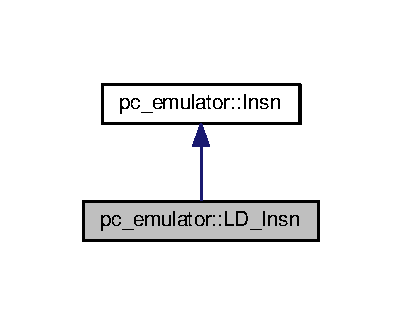
\includegraphics[width=193pt]{classpc__emulator_1_1LD__Insn__inherit__graph}
\end{center}
\end{figure}


Collaboration diagram for pc\+\_\+emulator\+:\+:L\+D\+\_\+\+Insn\+:
\nopagebreak
\begin{figure}[H]
\begin{center}
\leavevmode
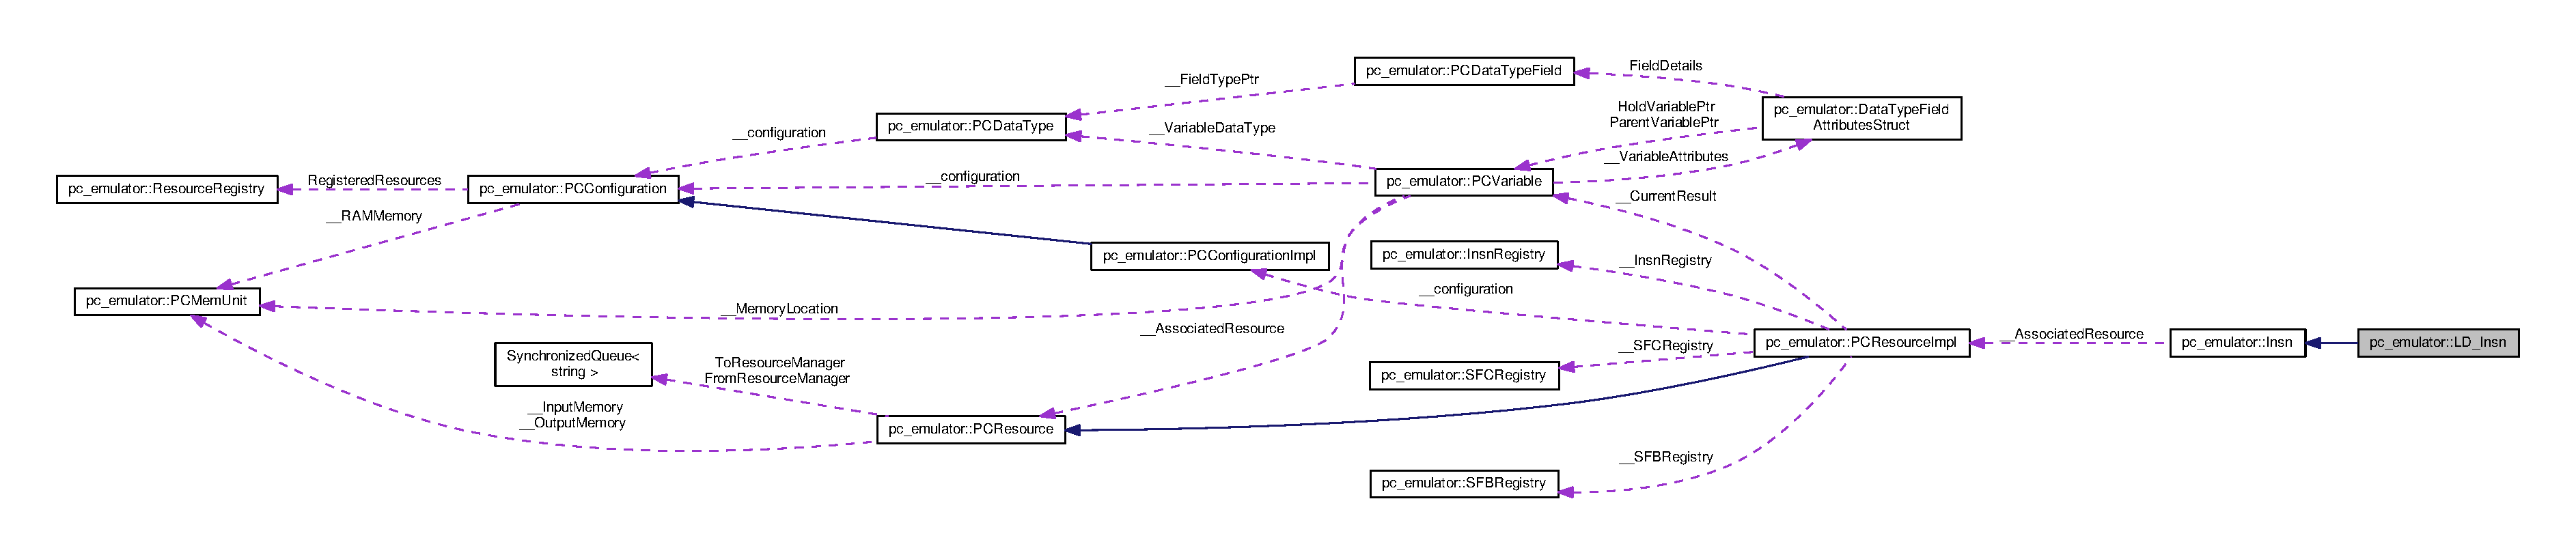
\includegraphics[width=350pt]{classpc__emulator_1_1LD__Insn__coll__graph}
\end{center}
\end{figure}
\subsection*{Public Member Functions}
\begin{DoxyCompactItemize}
\item 
{\bfseries L\+D\+\_\+\+Insn} (\hyperlink{classpc__emulator_1_1PCResourceImpl}{P\+C\+Resource\+Impl} $\ast$Associated\+Resource, bool is\+Negated)\hypertarget{classpc__emulator_1_1LD__Insn_a47dec0b27455300c6c921cef1d99fb78}{}\label{classpc__emulator_1_1LD__Insn_a47dec0b27455300c6c921cef1d99fb78}

\item 
void \hyperlink{classpc__emulator_1_1LD__Insn_a3afc230f457185fefc9f2297d8ab5c29}{Execute} (\hyperlink{classpc__emulator_1_1PCVariable}{P\+C\+Variable} $\ast$Current\+Result, std\+::vector$<$ \hyperlink{classpc__emulator_1_1PCVariable}{P\+C\+Variable} $\ast$ $>$ \&Operands)
\begin{DoxyCompactList}\small\item\em Called to execute the instruction. \end{DoxyCompactList}\end{DoxyCompactItemize}
\subsection*{Additional Inherited Members}


\subsection{Detailed Description}
Load instruction. 

\subsection{Member Function Documentation}
\index{pc\+\_\+emulator\+::\+L\+D\+\_\+\+Insn@{pc\+\_\+emulator\+::\+L\+D\+\_\+\+Insn}!Execute@{Execute}}
\index{Execute@{Execute}!pc\+\_\+emulator\+::\+L\+D\+\_\+\+Insn@{pc\+\_\+emulator\+::\+L\+D\+\_\+\+Insn}}
\subsubsection[{\texorpdfstring{Execute(\+P\+C\+Variable $\ast$\+Current\+Result, std\+::vector$<$ P\+C\+Variable $\ast$ $>$ \&\+Operands)}{Execute(PCVariable *CurrentResult, std::vector< PCVariable * > &Operands)}}]{\setlength{\rightskip}{0pt plus 5cm}void pc\+\_\+emulator\+::\+L\+D\+\_\+\+Insn\+::\+Execute (
\begin{DoxyParamCaption}
\item[{{\bf P\+C\+Variable} $\ast$}]{Current\+Result, }
\item[{std\+::vector$<$ {\bf P\+C\+Variable} $\ast$ $>$ \&}]{Operands}
\end{DoxyParamCaption}
)\hspace{0.3cm}{\ttfamily [virtual]}}\hypertarget{classpc__emulator_1_1LD__Insn_a3afc230f457185fefc9f2297d8ab5c29}{}\label{classpc__emulator_1_1LD__Insn_a3afc230f457185fefc9f2297d8ab5c29}


Called to execute the instruction. 


\begin{DoxyParams}{Parameters}
{\em Current\+Result} & The Current\+Result register of the task executing this \hyperlink{classpc__emulator_1_1Insn}{Insn} \\
\hline
{\em Operands} & Operands to the instruction \\
\hline
\end{DoxyParams}


Implements \hyperlink{classpc__emulator_1_1Insn_a103d27030e872a799e313df16c1f3d66}{pc\+\_\+emulator\+::\+Insn}.



The documentation for this class was generated from the following file\+:\begin{DoxyCompactItemize}
\item 
src/pc\+\_\+emulator/include/insns/ld\+\_\+insn.\+h\end{DoxyCompactItemize}

\hypertarget{classpc__emulator_1_1LE__Insn}{}\section{pc\+\_\+emulator\+:\+:L\+E\+\_\+\+Insn Class Reference}
\label{classpc__emulator_1_1LE__Insn}\index{pc\+\_\+emulator\+::\+L\+E\+\_\+\+Insn@{pc\+\_\+emulator\+::\+L\+E\+\_\+\+Insn}}


Lesser than or equal instruction.  




{\ttfamily \#include $<$le\+\_\+insn.\+h$>$}



Inheritance diagram for pc\+\_\+emulator\+:\+:L\+E\+\_\+\+Insn\+:\nopagebreak
\begin{figure}[H]
\begin{center}
\leavevmode
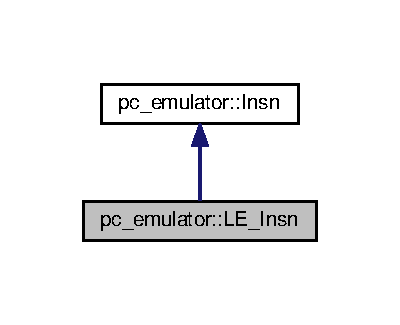
\includegraphics[width=192pt]{classpc__emulator_1_1LE__Insn__inherit__graph}
\end{center}
\end{figure}


Collaboration diagram for pc\+\_\+emulator\+:\+:L\+E\+\_\+\+Insn\+:\nopagebreak
\begin{figure}[H]
\begin{center}
\leavevmode
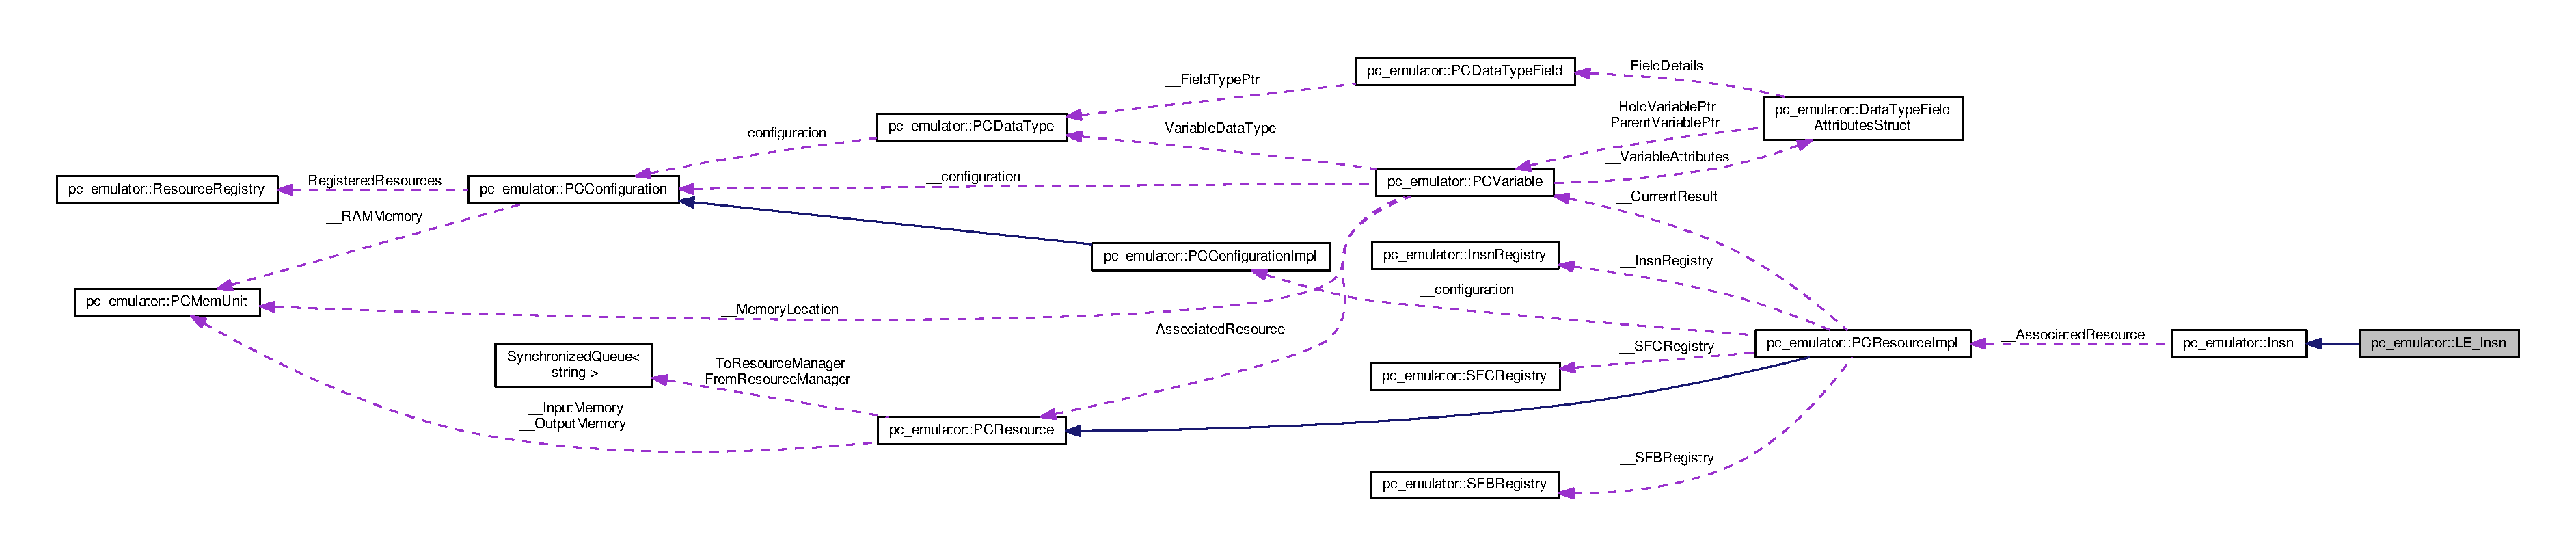
\includegraphics[width=350pt]{classpc__emulator_1_1LE__Insn__coll__graph}
\end{center}
\end{figure}
\subsection*{Public Member Functions}
\begin{DoxyCompactItemize}
\item 
{\bfseries L\+E\+\_\+\+Insn} (\hyperlink{classpc__emulator_1_1PCResourceImpl}{P\+C\+Resource\+Impl} $\ast$Associated\+Resource, bool is\+Negated)\hypertarget{classpc__emulator_1_1LE__Insn_a2fd32e06c101d75f9e6371a25e5b7a6b}{}\label{classpc__emulator_1_1LE__Insn_a2fd32e06c101d75f9e6371a25e5b7a6b}

\item 
void \hyperlink{classpc__emulator_1_1LE__Insn_a338cea25547481dd6ee9a62569f9bbaf}{Execute} (\hyperlink{classpc__emulator_1_1PCVariable}{P\+C\+Variable} $\ast$Current\+Result, std\+::vector$<$ \hyperlink{classpc__emulator_1_1PCVariable}{P\+C\+Variable} $\ast$ $>$ \&Operands)
\begin{DoxyCompactList}\small\item\em Called to execute the instruction. \end{DoxyCompactList}\end{DoxyCompactItemize}
\subsection*{Additional Inherited Members}


\subsection{Detailed Description}
Lesser than or equal instruction. 

\subsection{Member Function Documentation}
\index{pc\+\_\+emulator\+::\+L\+E\+\_\+\+Insn@{pc\+\_\+emulator\+::\+L\+E\+\_\+\+Insn}!Execute@{Execute}}
\index{Execute@{Execute}!pc\+\_\+emulator\+::\+L\+E\+\_\+\+Insn@{pc\+\_\+emulator\+::\+L\+E\+\_\+\+Insn}}
\subsubsection[{\texorpdfstring{Execute(\+P\+C\+Variable $\ast$\+Current\+Result, std\+::vector$<$ P\+C\+Variable $\ast$ $>$ \&\+Operands)}{Execute(PCVariable *CurrentResult, std::vector< PCVariable * > &Operands)}}]{\setlength{\rightskip}{0pt plus 5cm}void pc\+\_\+emulator\+::\+L\+E\+\_\+\+Insn\+::\+Execute (
\begin{DoxyParamCaption}
\item[{{\bf P\+C\+Variable} $\ast$}]{Current\+Result, }
\item[{std\+::vector$<$ {\bf P\+C\+Variable} $\ast$ $>$ \&}]{Operands}
\end{DoxyParamCaption}
)\hspace{0.3cm}{\ttfamily [virtual]}}\hypertarget{classpc__emulator_1_1LE__Insn_a338cea25547481dd6ee9a62569f9bbaf}{}\label{classpc__emulator_1_1LE__Insn_a338cea25547481dd6ee9a62569f9bbaf}


Called to execute the instruction. 


\begin{DoxyParams}{Parameters}
{\em Current\+Result} & The Current\+Result register of the task executing this \hyperlink{classpc__emulator_1_1Insn}{Insn} \\
\hline
{\em Operands} & Operands to the instruction \\
\hline
\end{DoxyParams}


Implements \hyperlink{classpc__emulator_1_1Insn_a103d27030e872a799e313df16c1f3d66}{pc\+\_\+emulator\+::\+Insn}.



The documentation for this class was generated from the following file\+:\begin{DoxyCompactItemize}
\item 
src/pc\+\_\+emulator/include/insns/le\+\_\+insn.\+h\end{DoxyCompactItemize}

\hypertarget{classpc__emulator_1_1LIMIT}{}\section{pc\+\_\+emulator\+:\+:L\+I\+M\+IT Class Reference}
\label{classpc__emulator_1_1LIMIT}\index{pc\+\_\+emulator\+::\+L\+I\+M\+IT@{pc\+\_\+emulator\+::\+L\+I\+M\+IT}}


Definition of \hyperlink{classpc__emulator_1_1LIMIT}{L\+I\+M\+IT} \hyperlink{classpc__emulator_1_1SFC}{S\+FC}.  




{\ttfamily \#include $<$limit.\+h$>$}



Inheritance diagram for pc\+\_\+emulator\+:\+:L\+I\+M\+IT\+:\nopagebreak
\begin{figure}[H]
\begin{center}
\leavevmode
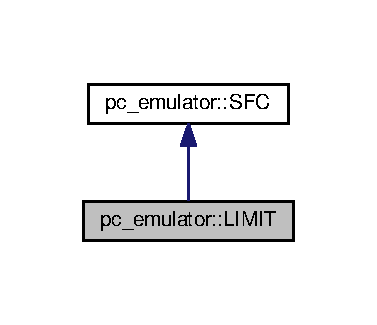
\includegraphics[width=181pt]{classpc__emulator_1_1LIMIT__inherit__graph}
\end{center}
\end{figure}


Collaboration diagram for pc\+\_\+emulator\+:\+:L\+I\+M\+IT\+:\nopagebreak
\begin{figure}[H]
\begin{center}
\leavevmode
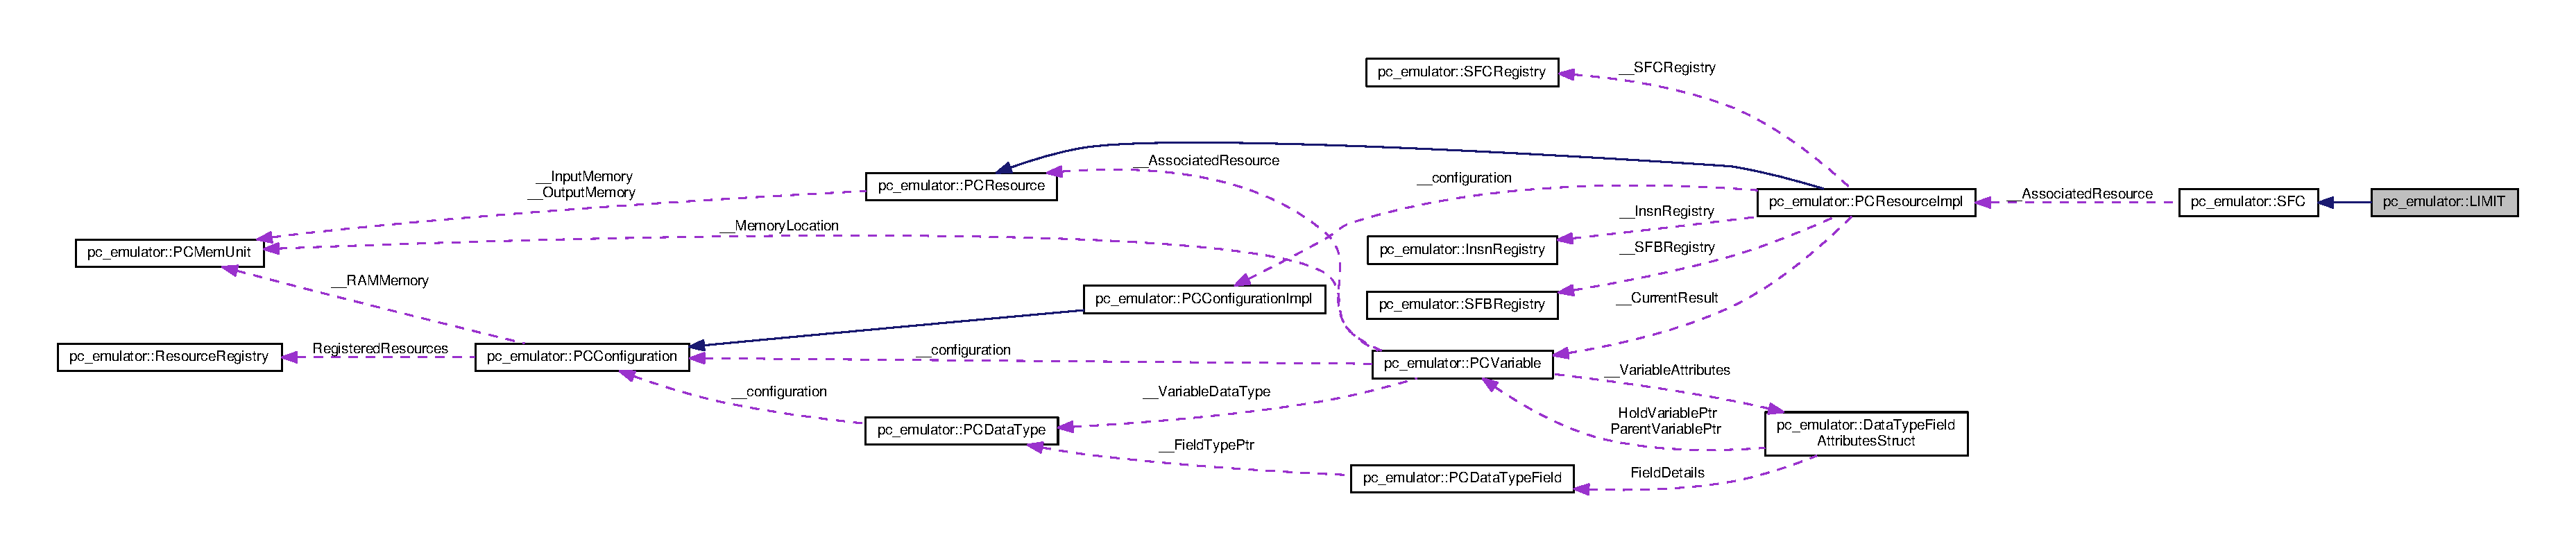
\includegraphics[width=350pt]{classpc__emulator_1_1LIMIT__coll__graph}
\end{center}
\end{figure}
\subsection*{Public Member Functions}
\begin{DoxyCompactItemize}
\item 
{\bfseries L\+I\+M\+IT} (\hyperlink{classpc__emulator_1_1PCResourceImpl}{P\+C\+Resource\+Impl} $\ast$Associated\+Resource)\hypertarget{classpc__emulator_1_1LIMIT_ae91b9b94f280081dae42680cdf7d11b5}{}\label{classpc__emulator_1_1LIMIT_ae91b9b94f280081dae42680cdf7d11b5}

\item 
void \hyperlink{classpc__emulator_1_1LIMIT_af8015be356d3994def6ee0bf67984bb3}{Execute} (\hyperlink{classpc__emulator_1_1PCVariable}{P\+C\+Variable} $\ast$Current\+Result, std\+::vector$<$ \hyperlink{classpc__emulator_1_1PCVariable}{P\+C\+Variable} $\ast$ $>$ \&Operands)
\begin{DoxyCompactList}\small\item\em Called to execute the sfc. \end{DoxyCompactList}\end{DoxyCompactItemize}
\subsection*{Additional Inherited Members}


\subsection{Detailed Description}
Definition of \hyperlink{classpc__emulator_1_1LIMIT}{L\+I\+M\+IT} \hyperlink{classpc__emulator_1_1SFC}{S\+FC}. 

\subsection{Member Function Documentation}
\index{pc\+\_\+emulator\+::\+L\+I\+M\+IT@{pc\+\_\+emulator\+::\+L\+I\+M\+IT}!Execute@{Execute}}
\index{Execute@{Execute}!pc\+\_\+emulator\+::\+L\+I\+M\+IT@{pc\+\_\+emulator\+::\+L\+I\+M\+IT}}
\subsubsection[{\texorpdfstring{Execute(\+P\+C\+Variable $\ast$\+Current\+Result, std\+::vector$<$ P\+C\+Variable $\ast$ $>$ \&\+Operands)}{Execute(PCVariable *CurrentResult, std::vector< PCVariable * > &Operands)}}]{\setlength{\rightskip}{0pt plus 5cm}void pc\+\_\+emulator\+::\+L\+I\+M\+I\+T\+::\+Execute (
\begin{DoxyParamCaption}
\item[{{\bf P\+C\+Variable} $\ast$}]{Current\+Result, }
\item[{std\+::vector$<$ {\bf P\+C\+Variable} $\ast$ $>$ \&}]{Operands}
\end{DoxyParamCaption}
)\hspace{0.3cm}{\ttfamily [virtual]}}\hypertarget{classpc__emulator_1_1LIMIT_af8015be356d3994def6ee0bf67984bb3}{}\label{classpc__emulator_1_1LIMIT_af8015be356d3994def6ee0bf67984bb3}


Called to execute the sfc. 


\begin{DoxyParams}{Parameters}
{\em Current\+Result} & The Current\+Result register of the task executing this \hyperlink{classpc__emulator_1_1SFC}{S\+FC} \\
\hline
{\em Operands} & Operands to the sfc \\
\hline
\end{DoxyParams}


Implements \hyperlink{classpc__emulator_1_1SFC_ab206c80fc0e429c56672b4f6a0ca8635}{pc\+\_\+emulator\+::\+S\+FC}.



The documentation for this class was generated from the following file\+:\begin{DoxyCompactItemize}
\item 
src/pc\+\_\+emulator/include/sfc/limit.\+h\end{DoxyCompactItemize}

\hypertarget{classpc__emulator_1_1LN}{}\section{pc\+\_\+emulator\+:\+:LN Class Reference}
\label{classpc__emulator_1_1LN}\index{pc\+\_\+emulator\+::\+LN@{pc\+\_\+emulator\+::\+LN}}


Definition of \hyperlink{classpc__emulator_1_1LN}{LN} \hyperlink{classpc__emulator_1_1SFC}{S\+FC}.  




{\ttfamily \#include $<$ln.\+h$>$}



Inheritance diagram for pc\+\_\+emulator\+:\+:LN\+:\nopagebreak
\begin{figure}[H]
\begin{center}
\leavevmode
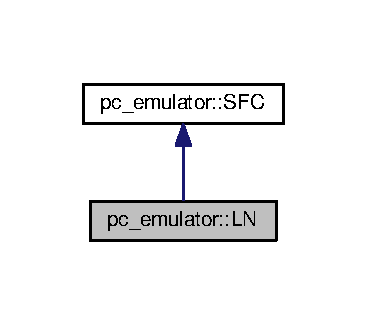
\includegraphics[width=176pt]{classpc__emulator_1_1LN__inherit__graph}
\end{center}
\end{figure}


Collaboration diagram for pc\+\_\+emulator\+:\+:LN\+:\nopagebreak
\begin{figure}[H]
\begin{center}
\leavevmode
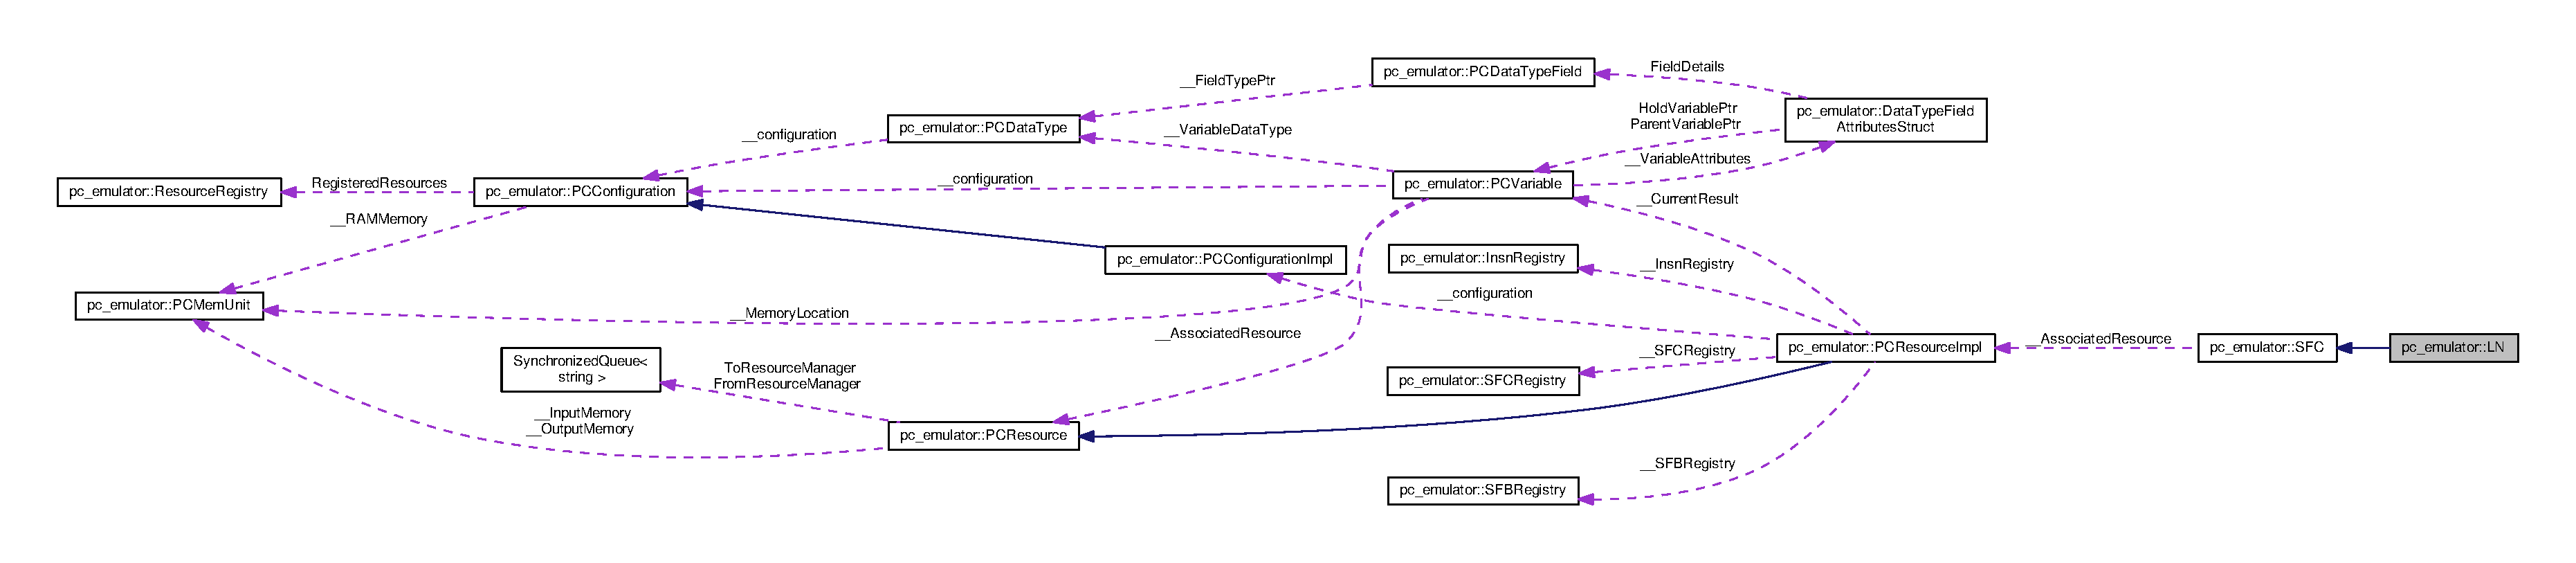
\includegraphics[width=350pt]{classpc__emulator_1_1LN__coll__graph}
\end{center}
\end{figure}
\subsection*{Public Member Functions}
\begin{DoxyCompactItemize}
\item 
{\bfseries LN} (\hyperlink{classpc__emulator_1_1PCResourceImpl}{P\+C\+Resource\+Impl} $\ast$Associated\+Resource)\hypertarget{classpc__emulator_1_1LN_a09d3c62f189f5b9b3ad2d8ae21b31f28}{}\label{classpc__emulator_1_1LN_a09d3c62f189f5b9b3ad2d8ae21b31f28}

\item 
void \hyperlink{classpc__emulator_1_1LN_ae132a2caf03e39d1984a3b4e9f7be374}{Execute} (\hyperlink{classpc__emulator_1_1PCVariable}{P\+C\+Variable} $\ast$Current\+Result, std\+::vector$<$ \hyperlink{classpc__emulator_1_1PCVariable}{P\+C\+Variable} $\ast$ $>$ \&Operands)
\begin{DoxyCompactList}\small\item\em Called to execute the sfc. \end{DoxyCompactList}\end{DoxyCompactItemize}
\subsection*{Additional Inherited Members}


\subsection{Detailed Description}
Definition of \hyperlink{classpc__emulator_1_1LN}{LN} \hyperlink{classpc__emulator_1_1SFC}{S\+FC}. 

\subsection{Member Function Documentation}
\index{pc\+\_\+emulator\+::\+LN@{pc\+\_\+emulator\+::\+LN}!Execute@{Execute}}
\index{Execute@{Execute}!pc\+\_\+emulator\+::\+LN@{pc\+\_\+emulator\+::\+LN}}
\subsubsection[{\texorpdfstring{Execute(\+P\+C\+Variable $\ast$\+Current\+Result, std\+::vector$<$ P\+C\+Variable $\ast$ $>$ \&\+Operands)}{Execute(PCVariable *CurrentResult, std::vector< PCVariable * > &Operands)}}]{\setlength{\rightskip}{0pt plus 5cm}void pc\+\_\+emulator\+::\+L\+N\+::\+Execute (
\begin{DoxyParamCaption}
\item[{{\bf P\+C\+Variable} $\ast$}]{Current\+Result, }
\item[{std\+::vector$<$ {\bf P\+C\+Variable} $\ast$ $>$ \&}]{Operands}
\end{DoxyParamCaption}
)\hspace{0.3cm}{\ttfamily [virtual]}}\hypertarget{classpc__emulator_1_1LN_ae132a2caf03e39d1984a3b4e9f7be374}{}\label{classpc__emulator_1_1LN_ae132a2caf03e39d1984a3b4e9f7be374}


Called to execute the sfc. 


\begin{DoxyParams}{Parameters}
{\em Current\+Result} & The Current\+Result register of the task executing this \hyperlink{classpc__emulator_1_1SFC}{S\+FC} \\
\hline
{\em Operands} & Operands to the sfc \\
\hline
\end{DoxyParams}


Implements \hyperlink{classpc__emulator_1_1SFC_ab206c80fc0e429c56672b4f6a0ca8635}{pc\+\_\+emulator\+::\+S\+FC}.



The documentation for this class was generated from the following file\+:\begin{DoxyCompactItemize}
\item 
src/pc\+\_\+emulator/include/sfc/ln.\+h\end{DoxyCompactItemize}

\hypertarget{classpc__emulator_1_1LOG}{}\section{pc\+\_\+emulator\+:\+:L\+OG Class Reference}
\label{classpc__emulator_1_1LOG}\index{pc\+\_\+emulator\+::\+L\+OG@{pc\+\_\+emulator\+::\+L\+OG}}


Definition of \hyperlink{classpc__emulator_1_1LOG}{L\+OG} \hyperlink{classpc__emulator_1_1SFC}{S\+FC}.  




{\ttfamily \#include $<$log.\+h$>$}



Inheritance diagram for pc\+\_\+emulator\+:\+:L\+OG\+:\nopagebreak
\begin{figure}[H]
\begin{center}
\leavevmode
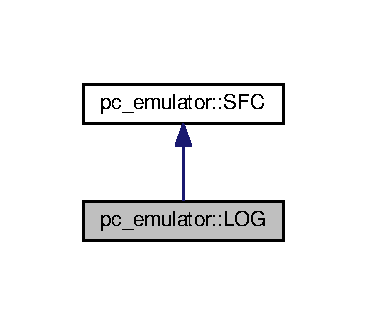
\includegraphics[width=176pt]{classpc__emulator_1_1LOG__inherit__graph}
\end{center}
\end{figure}


Collaboration diagram for pc\+\_\+emulator\+:\+:L\+OG\+:\nopagebreak
\begin{figure}[H]
\begin{center}
\leavevmode
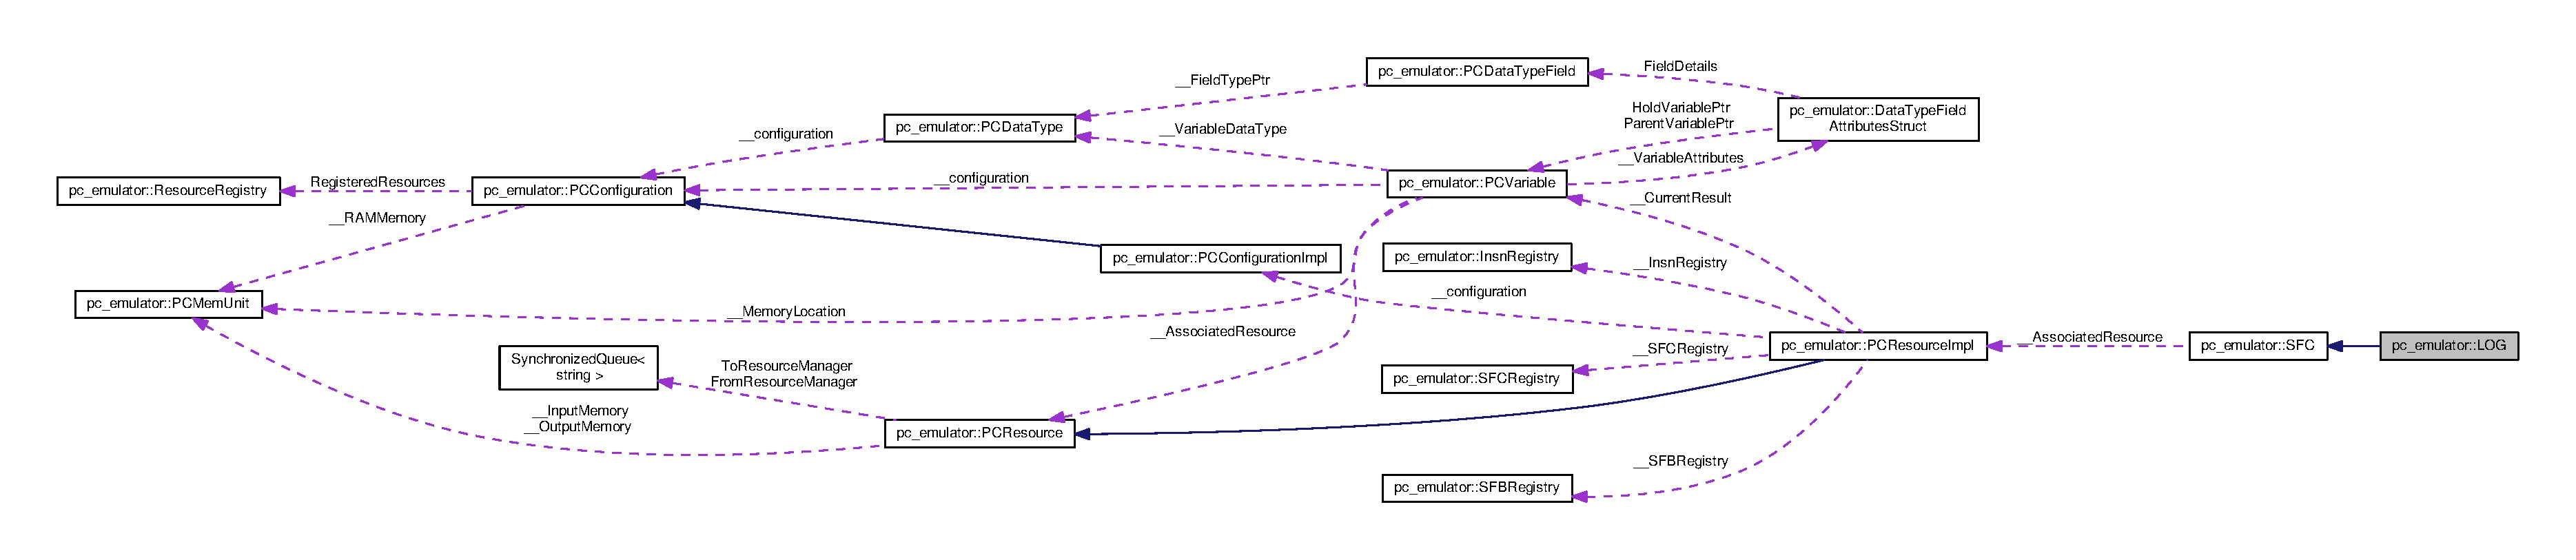
\includegraphics[width=350pt]{classpc__emulator_1_1LOG__coll__graph}
\end{center}
\end{figure}
\subsection*{Public Member Functions}
\begin{DoxyCompactItemize}
\item 
{\bfseries L\+OG} (\hyperlink{classpc__emulator_1_1PCResourceImpl}{P\+C\+Resource\+Impl} $\ast$Associated\+Resource)\hypertarget{classpc__emulator_1_1LOG_a3df9e42433e25af451792050ebec490b}{}\label{classpc__emulator_1_1LOG_a3df9e42433e25af451792050ebec490b}

\item 
void \hyperlink{classpc__emulator_1_1LOG_a47e1208a029c4f2c086e0cdc0ac8e215}{Execute} (\hyperlink{classpc__emulator_1_1PCVariable}{P\+C\+Variable} $\ast$Current\+Result, std\+::vector$<$ \hyperlink{classpc__emulator_1_1PCVariable}{P\+C\+Variable} $\ast$ $>$ \&Operands)
\begin{DoxyCompactList}\small\item\em Called to execute the sfc. \end{DoxyCompactList}\end{DoxyCompactItemize}
\subsection*{Additional Inherited Members}


\subsection{Detailed Description}
Definition of \hyperlink{classpc__emulator_1_1LOG}{L\+OG} \hyperlink{classpc__emulator_1_1SFC}{S\+FC}. 

\subsection{Member Function Documentation}
\index{pc\+\_\+emulator\+::\+L\+OG@{pc\+\_\+emulator\+::\+L\+OG}!Execute@{Execute}}
\index{Execute@{Execute}!pc\+\_\+emulator\+::\+L\+OG@{pc\+\_\+emulator\+::\+L\+OG}}
\subsubsection[{\texorpdfstring{Execute(\+P\+C\+Variable $\ast$\+Current\+Result, std\+::vector$<$ P\+C\+Variable $\ast$ $>$ \&\+Operands)}{Execute(PCVariable *CurrentResult, std::vector< PCVariable * > &Operands)}}]{\setlength{\rightskip}{0pt plus 5cm}void pc\+\_\+emulator\+::\+L\+O\+G\+::\+Execute (
\begin{DoxyParamCaption}
\item[{{\bf P\+C\+Variable} $\ast$}]{Current\+Result, }
\item[{std\+::vector$<$ {\bf P\+C\+Variable} $\ast$ $>$ \&}]{Operands}
\end{DoxyParamCaption}
)\hspace{0.3cm}{\ttfamily [virtual]}}\hypertarget{classpc__emulator_1_1LOG_a47e1208a029c4f2c086e0cdc0ac8e215}{}\label{classpc__emulator_1_1LOG_a47e1208a029c4f2c086e0cdc0ac8e215}


Called to execute the sfc. 


\begin{DoxyParams}{Parameters}
{\em Current\+Result} & The Current\+Result register of the task executing this \hyperlink{classpc__emulator_1_1SFC}{S\+FC} \\
\hline
{\em Operands} & Operands to the sfc \\
\hline
\end{DoxyParams}


Implements \hyperlink{classpc__emulator_1_1SFC_ab206c80fc0e429c56672b4f6a0ca8635}{pc\+\_\+emulator\+::\+S\+FC}.



The documentation for this class was generated from the following file\+:\begin{DoxyCompactItemize}
\item 
src/pc\+\_\+emulator/include/sfc/log.\+h\end{DoxyCompactItemize}

\hypertarget{classpc__emulator_1_1Logger}{}\section{pc\+\_\+emulator\+:\+:Logger Class Reference}
\label{classpc__emulator_1_1Logger}\index{pc\+\_\+emulator\+::\+Logger@{pc\+\_\+emulator\+::\+Logger}}


Class which can log information to stdout or to a file.  




{\ttfamily \#include $<$pc\+\_\+logger.\+h$>$}

\subsection*{Public Member Functions}
\begin{DoxyCompactItemize}
\item 
\hyperlink{classpc__emulator_1_1Logger_a26b4bcb02142f7e206c5f537b8d6367e}{Logger} (\hyperlink{classpc__emulator_1_1PCConfiguration}{P\+C\+Configuration} $\ast$configuration, std\+::string Log\+File, int Log\+Level)
\begin{DoxyCompactList}\small\item\em Constructor. \end{DoxyCompactList}\item 
void \hyperlink{classpc__emulator_1_1Logger_a30264e4e496bf8a2e74f56d57dc92067}{Log\+Message} (int Log\+Level, std\+::string Message)\hypertarget{classpc__emulator_1_1Logger_a30264e4e496bf8a2e74f56d57dc92067}{}\label{classpc__emulator_1_1Logger_a30264e4e496bf8a2e74f56d57dc92067}

\begin{DoxyCompactList}\small\item\em Logs a new message with the indicated Log\+Level. \end{DoxyCompactList}\item 
void \hyperlink{classpc__emulator_1_1Logger_a6a3838f5cdc03f802decfde8c06a3c9e}{Raise\+Exception} (std\+::string Error\+Message)\hypertarget{classpc__emulator_1_1Logger_a6a3838f5cdc03f802decfde8c06a3c9e}{}\label{classpc__emulator_1_1Logger_a6a3838f5cdc03f802decfde8c06a3c9e}

\begin{DoxyCompactList}\small\item\em Raises an exception which calls Shut\+Down. \end{DoxyCompactList}\item 
void \hyperlink{classpc__emulator_1_1Logger_a8df868de90c2149fefacbbbe0ff91539}{Shut\+Down} ()\hypertarget{classpc__emulator_1_1Logger_a8df868de90c2149fefacbbbe0ff91539}{}\label{classpc__emulator_1_1Logger_a8df868de90c2149fefacbbbe0ff91539}

\begin{DoxyCompactList}\small\item\em Shuts down the programmable controller. \end{DoxyCompactList}\end{DoxyCompactItemize}


\subsection{Detailed Description}
Class which can log information to stdout or to a file. 

\subsection{Constructor \& Destructor Documentation}
\index{pc\+\_\+emulator\+::\+Logger@{pc\+\_\+emulator\+::\+Logger}!Logger@{Logger}}
\index{Logger@{Logger}!pc\+\_\+emulator\+::\+Logger@{pc\+\_\+emulator\+::\+Logger}}
\subsubsection[{\texorpdfstring{Logger(\+P\+C\+Configuration $\ast$configuration, std\+::string Log\+File, int Log\+Level)}{Logger(PCConfiguration *configuration, std::string LogFile, int LogLevel)}}]{\setlength{\rightskip}{0pt plus 5cm}pc\+\_\+emulator\+::\+Logger\+::\+Logger (
\begin{DoxyParamCaption}
\item[{{\bf P\+C\+Configuration} $\ast$}]{configuration, }
\item[{std\+::string}]{Log\+File, }
\item[{int}]{Log\+Level}
\end{DoxyParamCaption}
)\hspace{0.3cm}{\ttfamily [inline]}}\hypertarget{classpc__emulator_1_1Logger_a26b4bcb02142f7e206c5f537b8d6367e}{}\label{classpc__emulator_1_1Logger_a26b4bcb02142f7e206c5f537b8d6367e}


Constructor. 


\begin{DoxyParams}{Parameters}
{\em configuration} & Associated configuration object \\
\hline
{\em Log\+File} & Full path to file. If empty, S\+T\+D\+O\+UT is chosen \\
\hline
{\em Log\+Level} & One of pc\+\_\+specification\+::\+Log\+Levels \\
\hline
\end{DoxyParams}


The documentation for this class was generated from the following file\+:\begin{DoxyCompactItemize}
\item 
src/pc\+\_\+emulator/include/pc\+\_\+logger.\+h\end{DoxyCompactItemize}

\hypertarget{classpc__emulator_1_1LT__Insn}{}\section{pc\+\_\+emulator\+:\+:L\+T\+\_\+\+Insn Class Reference}
\label{classpc__emulator_1_1LT__Insn}\index{pc\+\_\+emulator\+::\+L\+T\+\_\+\+Insn@{pc\+\_\+emulator\+::\+L\+T\+\_\+\+Insn}}


Lesser than instruction.  




{\ttfamily \#include $<$lt\+\_\+insn.\+h$>$}



Inheritance diagram for pc\+\_\+emulator\+:\+:L\+T\+\_\+\+Insn\+:
\nopagebreak
\begin{figure}[H]
\begin{center}
\leavevmode
\includegraphics[width=191pt]{classpc__emulator_1_1LT__Insn__inherit__graph}
\end{center}
\end{figure}


Collaboration diagram for pc\+\_\+emulator\+:\+:L\+T\+\_\+\+Insn\+:
\nopagebreak
\begin{figure}[H]
\begin{center}
\leavevmode
\includegraphics[width=350pt]{classpc__emulator_1_1LT__Insn__coll__graph}
\end{center}
\end{figure}
\subsection*{Public Member Functions}
\begin{DoxyCompactItemize}
\item 
{\bfseries L\+T\+\_\+\+Insn} (\hyperlink{classpc__emulator_1_1PCResourceImpl}{P\+C\+Resource\+Impl} $\ast$Associated\+Resource, bool is\+Negated)\hypertarget{classpc__emulator_1_1LT__Insn_a4397e3c95b9eddc37435643de15cfc67}{}\label{classpc__emulator_1_1LT__Insn_a4397e3c95b9eddc37435643de15cfc67}

\item 
void \hyperlink{classpc__emulator_1_1LT__Insn_a26d1613e7b8e042f10124d9e6758ff10}{Execute} (\hyperlink{classpc__emulator_1_1PCVariable}{P\+C\+Variable} $\ast$Current\+Result, std\+::vector$<$ \hyperlink{classpc__emulator_1_1PCVariable}{P\+C\+Variable} $\ast$ $>$ \&Operands)
\begin{DoxyCompactList}\small\item\em Called to execute the instruction. \end{DoxyCompactList}\end{DoxyCompactItemize}
\subsection*{Additional Inherited Members}


\subsection{Detailed Description}
Lesser than instruction. 

\subsection{Member Function Documentation}
\index{pc\+\_\+emulator\+::\+L\+T\+\_\+\+Insn@{pc\+\_\+emulator\+::\+L\+T\+\_\+\+Insn}!Execute@{Execute}}
\index{Execute@{Execute}!pc\+\_\+emulator\+::\+L\+T\+\_\+\+Insn@{pc\+\_\+emulator\+::\+L\+T\+\_\+\+Insn}}
\subsubsection[{\texorpdfstring{Execute(\+P\+C\+Variable $\ast$\+Current\+Result, std\+::vector$<$ P\+C\+Variable $\ast$ $>$ \&\+Operands)}{Execute(PCVariable *CurrentResult, std::vector< PCVariable * > &Operands)}}]{\setlength{\rightskip}{0pt plus 5cm}void pc\+\_\+emulator\+::\+L\+T\+\_\+\+Insn\+::\+Execute (
\begin{DoxyParamCaption}
\item[{{\bf P\+C\+Variable} $\ast$}]{Current\+Result, }
\item[{std\+::vector$<$ {\bf P\+C\+Variable} $\ast$ $>$ \&}]{Operands}
\end{DoxyParamCaption}
)\hspace{0.3cm}{\ttfamily [virtual]}}\hypertarget{classpc__emulator_1_1LT__Insn_a26d1613e7b8e042f10124d9e6758ff10}{}\label{classpc__emulator_1_1LT__Insn_a26d1613e7b8e042f10124d9e6758ff10}


Called to execute the instruction. 


\begin{DoxyParams}{Parameters}
{\em Current\+Result} & The Current\+Result register of the task executing this \hyperlink{classpc__emulator_1_1Insn}{Insn} \\
\hline
{\em Operands} & Operands to the instruction \\
\hline
\end{DoxyParams}


Implements \hyperlink{classpc__emulator_1_1Insn_a103d27030e872a799e313df16c1f3d66}{pc\+\_\+emulator\+::\+Insn}.



The documentation for this class was generated from the following file\+:\begin{DoxyCompactItemize}
\item 
src/pc\+\_\+emulator/include/insns/lt\+\_\+insn.\+h\end{DoxyCompactItemize}

\hypertarget{classpc__emulator_1_1Max}{}\section{pc\+\_\+emulator\+:\+:Max Class Reference}
\label{classpc__emulator_1_1Max}\index{pc\+\_\+emulator\+::\+Max@{pc\+\_\+emulator\+::\+Max}}


Definition of M\+AX \hyperlink{classpc__emulator_1_1SFC}{S\+FC}.  




{\ttfamily \#include $<$max.\+h$>$}



Inheritance diagram for pc\+\_\+emulator\+:\+:Max\+:\nopagebreak
\begin{figure}[H]
\begin{center}
\leavevmode
\includegraphics[width=176pt]{classpc__emulator_1_1Max__inherit__graph}
\end{center}
\end{figure}


Collaboration diagram for pc\+\_\+emulator\+:\+:Max\+:\nopagebreak
\begin{figure}[H]
\begin{center}
\leavevmode
\includegraphics[width=350pt]{classpc__emulator_1_1Max__coll__graph}
\end{center}
\end{figure}
\subsection*{Public Member Functions}
\begin{DoxyCompactItemize}
\item 
{\bfseries Max} (\hyperlink{classpc__emulator_1_1PCResourceImpl}{P\+C\+Resource\+Impl} $\ast$Associated\+Resource)\hypertarget{classpc__emulator_1_1Max_a1582118d91f7682d21e250fb78c77303}{}\label{classpc__emulator_1_1Max_a1582118d91f7682d21e250fb78c77303}

\item 
void \hyperlink{classpc__emulator_1_1Max_a69f272b0595cb79620251b28a9711b74}{Execute} (\hyperlink{classpc__emulator_1_1PCVariable}{P\+C\+Variable} $\ast$Current\+Result, std\+::vector$<$ \hyperlink{classpc__emulator_1_1PCVariable}{P\+C\+Variable} $\ast$ $>$ \&Operands)
\begin{DoxyCompactList}\small\item\em Called to execute the sfc. \end{DoxyCompactList}\end{DoxyCompactItemize}
\subsection*{Additional Inherited Members}


\subsection{Detailed Description}
Definition of M\+AX \hyperlink{classpc__emulator_1_1SFC}{S\+FC}. 

\subsection{Member Function Documentation}
\index{pc\+\_\+emulator\+::\+Max@{pc\+\_\+emulator\+::\+Max}!Execute@{Execute}}
\index{Execute@{Execute}!pc\+\_\+emulator\+::\+Max@{pc\+\_\+emulator\+::\+Max}}
\subsubsection[{\texorpdfstring{Execute(\+P\+C\+Variable $\ast$\+Current\+Result, std\+::vector$<$ P\+C\+Variable $\ast$ $>$ \&\+Operands)}{Execute(PCVariable *CurrentResult, std::vector< PCVariable * > &Operands)}}]{\setlength{\rightskip}{0pt plus 5cm}void pc\+\_\+emulator\+::\+Max\+::\+Execute (
\begin{DoxyParamCaption}
\item[{{\bf P\+C\+Variable} $\ast$}]{Current\+Result, }
\item[{std\+::vector$<$ {\bf P\+C\+Variable} $\ast$ $>$ \&}]{Operands}
\end{DoxyParamCaption}
)\hspace{0.3cm}{\ttfamily [virtual]}}\hypertarget{classpc__emulator_1_1Max_a69f272b0595cb79620251b28a9711b74}{}\label{classpc__emulator_1_1Max_a69f272b0595cb79620251b28a9711b74}


Called to execute the sfc. 


\begin{DoxyParams}{Parameters}
{\em Current\+Result} & The Current\+Result register of the task executing this \hyperlink{classpc__emulator_1_1SFC}{S\+FC} \\
\hline
{\em Operands} & Operands to the sfc \\
\hline
\end{DoxyParams}


Implements \hyperlink{classpc__emulator_1_1SFC_ab206c80fc0e429c56672b4f6a0ca8635}{pc\+\_\+emulator\+::\+S\+FC}.



The documentation for this class was generated from the following file\+:\begin{DoxyCompactItemize}
\item 
src/pc\+\_\+emulator/include/sfc/max.\+h\end{DoxyCompactItemize}

\hypertarget{classpc__emulator_1_1Min}{}\section{pc\+\_\+emulator\+:\+:Min Class Reference}
\label{classpc__emulator_1_1Min}\index{pc\+\_\+emulator\+::\+Min@{pc\+\_\+emulator\+::\+Min}}


Definition of \hyperlink{classpc__emulator_1_1Min}{Min} \hyperlink{classpc__emulator_1_1SFC}{S\+FC}.  




{\ttfamily \#include $<$min.\+h$>$}



Inheritance diagram for pc\+\_\+emulator\+:\+:Min\+:
\nopagebreak
\begin{figure}[H]
\begin{center}
\leavevmode
\includegraphics[width=176pt]{classpc__emulator_1_1Min__inherit__graph}
\end{center}
\end{figure}


Collaboration diagram for pc\+\_\+emulator\+:\+:Min\+:
\nopagebreak
\begin{figure}[H]
\begin{center}
\leavevmode
\includegraphics[width=350pt]{classpc__emulator_1_1Min__coll__graph}
\end{center}
\end{figure}
\subsection*{Public Member Functions}
\begin{DoxyCompactItemize}
\item 
{\bfseries Min} (\hyperlink{classpc__emulator_1_1PCResourceImpl}{P\+C\+Resource\+Impl} $\ast$Associated\+Resource)\hypertarget{classpc__emulator_1_1Min_ad1c645fb7a9f9821e38f3ef03158f26e}{}\label{classpc__emulator_1_1Min_ad1c645fb7a9f9821e38f3ef03158f26e}

\item 
void \hyperlink{classpc__emulator_1_1Min_a514862be9783380e78e8079cae70dd04}{Execute} (\hyperlink{classpc__emulator_1_1PCVariable}{P\+C\+Variable} $\ast$Current\+Result, std\+::vector$<$ \hyperlink{classpc__emulator_1_1PCVariable}{P\+C\+Variable} $\ast$ $>$ \&Operands)
\begin{DoxyCompactList}\small\item\em Called to execute the sfc. \end{DoxyCompactList}\end{DoxyCompactItemize}
\subsection*{Additional Inherited Members}


\subsection{Detailed Description}
Definition of \hyperlink{classpc__emulator_1_1Min}{Min} \hyperlink{classpc__emulator_1_1SFC}{S\+FC}. 

\subsection{Member Function Documentation}
\index{pc\+\_\+emulator\+::\+Min@{pc\+\_\+emulator\+::\+Min}!Execute@{Execute}}
\index{Execute@{Execute}!pc\+\_\+emulator\+::\+Min@{pc\+\_\+emulator\+::\+Min}}
\subsubsection[{\texorpdfstring{Execute(\+P\+C\+Variable $\ast$\+Current\+Result, std\+::vector$<$ P\+C\+Variable $\ast$ $>$ \&\+Operands)}{Execute(PCVariable *CurrentResult, std::vector< PCVariable * > &Operands)}}]{\setlength{\rightskip}{0pt plus 5cm}void pc\+\_\+emulator\+::\+Min\+::\+Execute (
\begin{DoxyParamCaption}
\item[{{\bf P\+C\+Variable} $\ast$}]{Current\+Result, }
\item[{std\+::vector$<$ {\bf P\+C\+Variable} $\ast$ $>$ \&}]{Operands}
\end{DoxyParamCaption}
)\hspace{0.3cm}{\ttfamily [virtual]}}\hypertarget{classpc__emulator_1_1Min_a514862be9783380e78e8079cae70dd04}{}\label{classpc__emulator_1_1Min_a514862be9783380e78e8079cae70dd04}


Called to execute the sfc. 


\begin{DoxyParams}{Parameters}
{\em Current\+Result} & The Current\+Result register of the task executing this \hyperlink{classpc__emulator_1_1SFC}{S\+FC} \\
\hline
{\em Operands} & Operands to the sfc \\
\hline
\end{DoxyParams}


Implements \hyperlink{classpc__emulator_1_1SFC_ab206c80fc0e429c56672b4f6a0ca8635}{pc\+\_\+emulator\+::\+S\+FC}.



The documentation for this class was generated from the following file\+:\begin{DoxyCompactItemize}
\item 
src/pc\+\_\+emulator/include/sfc/min.\+h\end{DoxyCompactItemize}

\hypertarget{classpc__emulator_1_1MOD__Insn}{}\section{pc\+\_\+emulator\+:\+:M\+O\+D\+\_\+\+Insn Class Reference}
\label{classpc__emulator_1_1MOD__Insn}\index{pc\+\_\+emulator\+::\+M\+O\+D\+\_\+\+Insn@{pc\+\_\+emulator\+::\+M\+O\+D\+\_\+\+Insn}}


M\+OD instruction.  




{\ttfamily \#include $<$mod\+\_\+insn.\+h$>$}



Inheritance diagram for pc\+\_\+emulator\+:\+:M\+O\+D\+\_\+\+Insn\+:
\nopagebreak
\begin{figure}[H]
\begin{center}
\leavevmode
\includegraphics[width=203pt]{classpc__emulator_1_1MOD__Insn__inherit__graph}
\end{center}
\end{figure}


Collaboration diagram for pc\+\_\+emulator\+:\+:M\+O\+D\+\_\+\+Insn\+:
\nopagebreak
\begin{figure}[H]
\begin{center}
\leavevmode
\includegraphics[width=350pt]{classpc__emulator_1_1MOD__Insn__coll__graph}
\end{center}
\end{figure}
\subsection*{Public Member Functions}
\begin{DoxyCompactItemize}
\item 
{\bfseries M\+O\+D\+\_\+\+Insn} (\hyperlink{classpc__emulator_1_1PCResourceImpl}{P\+C\+Resource\+Impl} $\ast$Associated\+Resource, bool is\+Negated)\hypertarget{classpc__emulator_1_1MOD__Insn_afdd62b922a9891b66d9de37088d74a2b}{}\label{classpc__emulator_1_1MOD__Insn_afdd62b922a9891b66d9de37088d74a2b}

\item 
void \hyperlink{classpc__emulator_1_1MOD__Insn_ad6555ef4921d88fa8ef48c37c602b0fd}{Execute} (\hyperlink{classpc__emulator_1_1PCVariable}{P\+C\+Variable} $\ast$Current\+Result, std\+::vector$<$ \hyperlink{classpc__emulator_1_1PCVariable}{P\+C\+Variable} $\ast$ $>$ \&Operands)
\begin{DoxyCompactList}\small\item\em Called to execute the instruction. \end{DoxyCompactList}\end{DoxyCompactItemize}
\subsection*{Additional Inherited Members}


\subsection{Detailed Description}
M\+OD instruction. 

\subsection{Member Function Documentation}
\index{pc\+\_\+emulator\+::\+M\+O\+D\+\_\+\+Insn@{pc\+\_\+emulator\+::\+M\+O\+D\+\_\+\+Insn}!Execute@{Execute}}
\index{Execute@{Execute}!pc\+\_\+emulator\+::\+M\+O\+D\+\_\+\+Insn@{pc\+\_\+emulator\+::\+M\+O\+D\+\_\+\+Insn}}
\subsubsection[{\texorpdfstring{Execute(\+P\+C\+Variable $\ast$\+Current\+Result, std\+::vector$<$ P\+C\+Variable $\ast$ $>$ \&\+Operands)}{Execute(PCVariable *CurrentResult, std::vector< PCVariable * > &Operands)}}]{\setlength{\rightskip}{0pt plus 5cm}void pc\+\_\+emulator\+::\+M\+O\+D\+\_\+\+Insn\+::\+Execute (
\begin{DoxyParamCaption}
\item[{{\bf P\+C\+Variable} $\ast$}]{Current\+Result, }
\item[{std\+::vector$<$ {\bf P\+C\+Variable} $\ast$ $>$ \&}]{Operands}
\end{DoxyParamCaption}
)\hspace{0.3cm}{\ttfamily [virtual]}}\hypertarget{classpc__emulator_1_1MOD__Insn_ad6555ef4921d88fa8ef48c37c602b0fd}{}\label{classpc__emulator_1_1MOD__Insn_ad6555ef4921d88fa8ef48c37c602b0fd}


Called to execute the instruction. 


\begin{DoxyParams}{Parameters}
{\em Current\+Result} & The Current\+Result register of the task executing this \hyperlink{classpc__emulator_1_1Insn}{Insn} \\
\hline
{\em Operands} & Operands to the instruction \\
\hline
\end{DoxyParams}


Implements \hyperlink{classpc__emulator_1_1Insn_a103d27030e872a799e313df16c1f3d66}{pc\+\_\+emulator\+::\+Insn}.



The documentation for this class was generated from the following file\+:\begin{DoxyCompactItemize}
\item 
src/pc\+\_\+emulator/include/insns/mod\+\_\+insn.\+h\end{DoxyCompactItemize}

\hypertarget{classpc__emulator_1_1MUL__Insn}{}\section{pc\+\_\+emulator\+:\+:M\+U\+L\+\_\+\+Insn Class Reference}
\label{classpc__emulator_1_1MUL__Insn}\index{pc\+\_\+emulator\+::\+M\+U\+L\+\_\+\+Insn@{pc\+\_\+emulator\+::\+M\+U\+L\+\_\+\+Insn}}


Multiply instruction.  




{\ttfamily \#include $<$mul\+\_\+insn.\+h$>$}



Inheritance diagram for pc\+\_\+emulator\+:\+:M\+U\+L\+\_\+\+Insn\+:
\nopagebreak
\begin{figure}[H]
\begin{center}
\leavevmode
\includegraphics[width=201pt]{classpc__emulator_1_1MUL__Insn__inherit__graph}
\end{center}
\end{figure}


Collaboration diagram for pc\+\_\+emulator\+:\+:M\+U\+L\+\_\+\+Insn\+:
\nopagebreak
\begin{figure}[H]
\begin{center}
\leavevmode
\includegraphics[width=350pt]{classpc__emulator_1_1MUL__Insn__coll__graph}
\end{center}
\end{figure}
\subsection*{Public Member Functions}
\begin{DoxyCompactItemize}
\item 
{\bfseries M\+U\+L\+\_\+\+Insn} (\hyperlink{classpc__emulator_1_1PCResourceImpl}{P\+C\+Resource\+Impl} $\ast$Associated\+Resource, bool is\+Negated)\hypertarget{classpc__emulator_1_1MUL__Insn_ab728942edbb3a66a3873bf7adfced8d4}{}\label{classpc__emulator_1_1MUL__Insn_ab728942edbb3a66a3873bf7adfced8d4}

\item 
void \hyperlink{classpc__emulator_1_1MUL__Insn_a8575326e90b1bbdf1587a79ba575b733}{Execute} (\hyperlink{classpc__emulator_1_1PCVariable}{P\+C\+Variable} $\ast$Current\+Result, std\+::vector$<$ \hyperlink{classpc__emulator_1_1PCVariable}{P\+C\+Variable} $\ast$ $>$ \&Operands)
\begin{DoxyCompactList}\small\item\em Called to execute the instruction. \end{DoxyCompactList}\end{DoxyCompactItemize}
\subsection*{Additional Inherited Members}


\subsection{Detailed Description}
Multiply instruction. 

\subsection{Member Function Documentation}
\index{pc\+\_\+emulator\+::\+M\+U\+L\+\_\+\+Insn@{pc\+\_\+emulator\+::\+M\+U\+L\+\_\+\+Insn}!Execute@{Execute}}
\index{Execute@{Execute}!pc\+\_\+emulator\+::\+M\+U\+L\+\_\+\+Insn@{pc\+\_\+emulator\+::\+M\+U\+L\+\_\+\+Insn}}
\subsubsection[{\texorpdfstring{Execute(\+P\+C\+Variable $\ast$\+Current\+Result, std\+::vector$<$ P\+C\+Variable $\ast$ $>$ \&\+Operands)}{Execute(PCVariable *CurrentResult, std::vector< PCVariable * > &Operands)}}]{\setlength{\rightskip}{0pt plus 5cm}void pc\+\_\+emulator\+::\+M\+U\+L\+\_\+\+Insn\+::\+Execute (
\begin{DoxyParamCaption}
\item[{{\bf P\+C\+Variable} $\ast$}]{Current\+Result, }
\item[{std\+::vector$<$ {\bf P\+C\+Variable} $\ast$ $>$ \&}]{Operands}
\end{DoxyParamCaption}
)\hspace{0.3cm}{\ttfamily [virtual]}}\hypertarget{classpc__emulator_1_1MUL__Insn_a8575326e90b1bbdf1587a79ba575b733}{}\label{classpc__emulator_1_1MUL__Insn_a8575326e90b1bbdf1587a79ba575b733}


Called to execute the instruction. 


\begin{DoxyParams}{Parameters}
{\em Current\+Result} & The Current\+Result register of the task executing this \hyperlink{classpc__emulator_1_1Insn}{Insn} \\
\hline
{\em Operands} & Operands to the instruction \\
\hline
\end{DoxyParams}


Implements \hyperlink{classpc__emulator_1_1Insn_a103d27030e872a799e313df16c1f3d66}{pc\+\_\+emulator\+::\+Insn}.



The documentation for this class was generated from the following file\+:\begin{DoxyCompactItemize}
\item 
src/pc\+\_\+emulator/include/insns/mul\+\_\+insn.\+h\end{DoxyCompactItemize}

\hypertarget{classpc__emulator_1_1MUX}{}\section{pc\+\_\+emulator\+:\+:M\+UX Class Reference}
\label{classpc__emulator_1_1MUX}\index{pc\+\_\+emulator\+::\+M\+UX@{pc\+\_\+emulator\+::\+M\+UX}}


Definition of \hyperlink{classpc__emulator_1_1MUX}{M\+UX} \hyperlink{classpc__emulator_1_1SFC}{S\+FC}.  




{\ttfamily \#include $<$mux.\+h$>$}



Inheritance diagram for pc\+\_\+emulator\+:\+:M\+UX\+:\nopagebreak
\begin{figure}[H]
\begin{center}
\leavevmode
\includegraphics[width=178pt]{classpc__emulator_1_1MUX__inherit__graph}
\end{center}
\end{figure}


Collaboration diagram for pc\+\_\+emulator\+:\+:M\+UX\+:\nopagebreak
\begin{figure}[H]
\begin{center}
\leavevmode
\includegraphics[width=350pt]{classpc__emulator_1_1MUX__coll__graph}
\end{center}
\end{figure}
\subsection*{Public Member Functions}
\begin{DoxyCompactItemize}
\item 
{\bfseries M\+UX} (\hyperlink{classpc__emulator_1_1PCResourceImpl}{P\+C\+Resource\+Impl} $\ast$Associated\+Resource)\hypertarget{classpc__emulator_1_1MUX_a0f3717c1cfc8d67ae5b46bdedbd25ba3}{}\label{classpc__emulator_1_1MUX_a0f3717c1cfc8d67ae5b46bdedbd25ba3}

\item 
void \hyperlink{classpc__emulator_1_1MUX_abae7cc0b591d2605033ce0aece5d291f}{Execute} (\hyperlink{classpc__emulator_1_1PCVariable}{P\+C\+Variable} $\ast$Current\+Result, std\+::vector$<$ \hyperlink{classpc__emulator_1_1PCVariable}{P\+C\+Variable} $\ast$ $>$ \&Operands)
\begin{DoxyCompactList}\small\item\em Called to execute the sfc. \end{DoxyCompactList}\end{DoxyCompactItemize}
\subsection*{Additional Inherited Members}


\subsection{Detailed Description}
Definition of \hyperlink{classpc__emulator_1_1MUX}{M\+UX} \hyperlink{classpc__emulator_1_1SFC}{S\+FC}. 

\subsection{Member Function Documentation}
\index{pc\+\_\+emulator\+::\+M\+UX@{pc\+\_\+emulator\+::\+M\+UX}!Execute@{Execute}}
\index{Execute@{Execute}!pc\+\_\+emulator\+::\+M\+UX@{pc\+\_\+emulator\+::\+M\+UX}}
\subsubsection[{\texorpdfstring{Execute(\+P\+C\+Variable $\ast$\+Current\+Result, std\+::vector$<$ P\+C\+Variable $\ast$ $>$ \&\+Operands)}{Execute(PCVariable *CurrentResult, std::vector< PCVariable * > &Operands)}}]{\setlength{\rightskip}{0pt plus 5cm}void pc\+\_\+emulator\+::\+M\+U\+X\+::\+Execute (
\begin{DoxyParamCaption}
\item[{{\bf P\+C\+Variable} $\ast$}]{Current\+Result, }
\item[{std\+::vector$<$ {\bf P\+C\+Variable} $\ast$ $>$ \&}]{Operands}
\end{DoxyParamCaption}
)\hspace{0.3cm}{\ttfamily [virtual]}}\hypertarget{classpc__emulator_1_1MUX_abae7cc0b591d2605033ce0aece5d291f}{}\label{classpc__emulator_1_1MUX_abae7cc0b591d2605033ce0aece5d291f}


Called to execute the sfc. 


\begin{DoxyParams}{Parameters}
{\em Current\+Result} & The Current\+Result register of the task executing this \hyperlink{classpc__emulator_1_1SFC}{S\+FC} \\
\hline
{\em Operands} & Operands to the sfc \\
\hline
\end{DoxyParams}


Implements \hyperlink{classpc__emulator_1_1SFC_ab206c80fc0e429c56672b4f6a0ca8635}{pc\+\_\+emulator\+::\+S\+FC}.



The documentation for this class was generated from the following file\+:\begin{DoxyCompactItemize}
\item 
src/pc\+\_\+emulator/include/sfc/mux.\+h\end{DoxyCompactItemize}

\hypertarget{classpc__emulator_1_1NE__Insn}{}\section{pc\+\_\+emulator\+:\+:N\+E\+\_\+\+Insn Class Reference}
\label{classpc__emulator_1_1NE__Insn}\index{pc\+\_\+emulator\+::\+N\+E\+\_\+\+Insn@{pc\+\_\+emulator\+::\+N\+E\+\_\+\+Insn}}


Test for not equal instruction.  




{\ttfamily \#include $<$ne\+\_\+insn.\+h$>$}



Inheritance diagram for pc\+\_\+emulator\+:\+:N\+E\+\_\+\+Insn\+:
\nopagebreak
\begin{figure}[H]
\begin{center}
\leavevmode
\includegraphics[width=194pt]{classpc__emulator_1_1NE__Insn__inherit__graph}
\end{center}
\end{figure}


Collaboration diagram for pc\+\_\+emulator\+:\+:N\+E\+\_\+\+Insn\+:
\nopagebreak
\begin{figure}[H]
\begin{center}
\leavevmode
\includegraphics[width=350pt]{classpc__emulator_1_1NE__Insn__coll__graph}
\end{center}
\end{figure}
\subsection*{Public Member Functions}
\begin{DoxyCompactItemize}
\item 
{\bfseries N\+E\+\_\+\+Insn} (\hyperlink{classpc__emulator_1_1PCResourceImpl}{P\+C\+Resource\+Impl} $\ast$Associated\+Resource, bool is\+Negated)\hypertarget{classpc__emulator_1_1NE__Insn_aa2faf3c7bfae0e56b138adaf71eee377}{}\label{classpc__emulator_1_1NE__Insn_aa2faf3c7bfae0e56b138adaf71eee377}

\item 
void \hyperlink{classpc__emulator_1_1NE__Insn_abd2edddfbc2fecbcde5e154293c40ebc}{Execute} (\hyperlink{classpc__emulator_1_1PCVariable}{P\+C\+Variable} $\ast$Current\+Result, std\+::vector$<$ \hyperlink{classpc__emulator_1_1PCVariable}{P\+C\+Variable} $\ast$ $>$ \&Operands)
\begin{DoxyCompactList}\small\item\em Called to execute the instruction. \end{DoxyCompactList}\end{DoxyCompactItemize}
\subsection*{Additional Inherited Members}


\subsection{Detailed Description}
Test for not equal instruction. 

\subsection{Member Function Documentation}
\index{pc\+\_\+emulator\+::\+N\+E\+\_\+\+Insn@{pc\+\_\+emulator\+::\+N\+E\+\_\+\+Insn}!Execute@{Execute}}
\index{Execute@{Execute}!pc\+\_\+emulator\+::\+N\+E\+\_\+\+Insn@{pc\+\_\+emulator\+::\+N\+E\+\_\+\+Insn}}
\subsubsection[{\texorpdfstring{Execute(\+P\+C\+Variable $\ast$\+Current\+Result, std\+::vector$<$ P\+C\+Variable $\ast$ $>$ \&\+Operands)}{Execute(PCVariable *CurrentResult, std::vector< PCVariable * > &Operands)}}]{\setlength{\rightskip}{0pt plus 5cm}void pc\+\_\+emulator\+::\+N\+E\+\_\+\+Insn\+::\+Execute (
\begin{DoxyParamCaption}
\item[{{\bf P\+C\+Variable} $\ast$}]{Current\+Result, }
\item[{std\+::vector$<$ {\bf P\+C\+Variable} $\ast$ $>$ \&}]{Operands}
\end{DoxyParamCaption}
)\hspace{0.3cm}{\ttfamily [virtual]}}\hypertarget{classpc__emulator_1_1NE__Insn_abd2edddfbc2fecbcde5e154293c40ebc}{}\label{classpc__emulator_1_1NE__Insn_abd2edddfbc2fecbcde5e154293c40ebc}


Called to execute the instruction. 


\begin{DoxyParams}{Parameters}
{\em Current\+Result} & The Current\+Result register of the task executing this \hyperlink{classpc__emulator_1_1Insn}{Insn} \\
\hline
{\em Operands} & Operands to the instruction \\
\hline
\end{DoxyParams}


Implements \hyperlink{classpc__emulator_1_1Insn_a103d27030e872a799e313df16c1f3d66}{pc\+\_\+emulator\+::\+Insn}.



The documentation for this class was generated from the following file\+:\begin{DoxyCompactItemize}
\item 
src/pc\+\_\+emulator/include/insns/ne\+\_\+insn.\+h\end{DoxyCompactItemize}

\hypertarget{classpc__emulator_1_1NOT__Insn}{}\section{pc\+\_\+emulator\+:\+:N\+O\+T\+\_\+\+Insn Class Reference}
\label{classpc__emulator_1_1NOT__Insn}\index{pc\+\_\+emulator\+::\+N\+O\+T\+\_\+\+Insn@{pc\+\_\+emulator\+::\+N\+O\+T\+\_\+\+Insn}}


N\+OT instruction.  




{\ttfamily \#include $<$not\+\_\+insn.\+h$>$}



Inheritance diagram for pc\+\_\+emulator\+:\+:N\+O\+T\+\_\+\+Insn\+:\nopagebreak
\begin{figure}[H]
\begin{center}
\leavevmode
\includegraphics[width=201pt]{classpc__emulator_1_1NOT__Insn__inherit__graph}
\end{center}
\end{figure}


Collaboration diagram for pc\+\_\+emulator\+:\+:N\+O\+T\+\_\+\+Insn\+:\nopagebreak
\begin{figure}[H]
\begin{center}
\leavevmode
\includegraphics[width=350pt]{classpc__emulator_1_1NOT__Insn__coll__graph}
\end{center}
\end{figure}
\subsection*{Public Member Functions}
\begin{DoxyCompactItemize}
\item 
{\bfseries N\+O\+T\+\_\+\+Insn} (\hyperlink{classpc__emulator_1_1PCResourceImpl}{P\+C\+Resource\+Impl} $\ast$Associated\+Resource, bool is\+Negated)\hypertarget{classpc__emulator_1_1NOT__Insn_a2dd7e20fbdd50ac413daa1ee9aa95917}{}\label{classpc__emulator_1_1NOT__Insn_a2dd7e20fbdd50ac413daa1ee9aa95917}

\item 
void \hyperlink{classpc__emulator_1_1NOT__Insn_a26832f4fb932e0162f2d80ccdbbd5983}{Execute} (\hyperlink{classpc__emulator_1_1PCVariable}{P\+C\+Variable} $\ast$Current\+Result, std\+::vector$<$ \hyperlink{classpc__emulator_1_1PCVariable}{P\+C\+Variable} $\ast$ $>$ \&Operands)
\begin{DoxyCompactList}\small\item\em Called to execute the instruction. \end{DoxyCompactList}\end{DoxyCompactItemize}
\subsection*{Additional Inherited Members}


\subsection{Detailed Description}
N\+OT instruction. 

\subsection{Member Function Documentation}
\index{pc\+\_\+emulator\+::\+N\+O\+T\+\_\+\+Insn@{pc\+\_\+emulator\+::\+N\+O\+T\+\_\+\+Insn}!Execute@{Execute}}
\index{Execute@{Execute}!pc\+\_\+emulator\+::\+N\+O\+T\+\_\+\+Insn@{pc\+\_\+emulator\+::\+N\+O\+T\+\_\+\+Insn}}
\subsubsection[{\texorpdfstring{Execute(\+P\+C\+Variable $\ast$\+Current\+Result, std\+::vector$<$ P\+C\+Variable $\ast$ $>$ \&\+Operands)}{Execute(PCVariable *CurrentResult, std::vector< PCVariable * > &Operands)}}]{\setlength{\rightskip}{0pt plus 5cm}void pc\+\_\+emulator\+::\+N\+O\+T\+\_\+\+Insn\+::\+Execute (
\begin{DoxyParamCaption}
\item[{{\bf P\+C\+Variable} $\ast$}]{Current\+Result, }
\item[{std\+::vector$<$ {\bf P\+C\+Variable} $\ast$ $>$ \&}]{Operands}
\end{DoxyParamCaption}
)\hspace{0.3cm}{\ttfamily [virtual]}}\hypertarget{classpc__emulator_1_1NOT__Insn_a26832f4fb932e0162f2d80ccdbbd5983}{}\label{classpc__emulator_1_1NOT__Insn_a26832f4fb932e0162f2d80ccdbbd5983}


Called to execute the instruction. 


\begin{DoxyParams}{Parameters}
{\em Current\+Result} & The Current\+Result register of the task executing this \hyperlink{classpc__emulator_1_1Insn}{Insn} \\
\hline
{\em Operands} & Operands to the instruction \\
\hline
\end{DoxyParams}


Implements \hyperlink{classpc__emulator_1_1Insn_a103d27030e872a799e313df16c1f3d66}{pc\+\_\+emulator\+::\+Insn}.



The documentation for this class was generated from the following file\+:\begin{DoxyCompactItemize}
\item 
src/pc\+\_\+emulator/include/insns/not\+\_\+insn.\+h\end{DoxyCompactItemize}

\hypertarget{classpc__emulator_1_1OR__Insn}{}\section{pc\+\_\+emulator\+:\+:O\+R\+\_\+\+Insn Class Reference}
\label{classpc__emulator_1_1OR__Insn}\index{pc\+\_\+emulator\+::\+O\+R\+\_\+\+Insn@{pc\+\_\+emulator\+::\+O\+R\+\_\+\+Insn}}


Bitwise OR instruction.  




{\ttfamily \#include $<$or\+\_\+insn.\+h$>$}



Inheritance diagram for pc\+\_\+emulator\+:\+:O\+R\+\_\+\+Insn\+:\nopagebreak
\begin{figure}[H]
\begin{center}
\leavevmode
\includegraphics[width=195pt]{classpc__emulator_1_1OR__Insn__inherit__graph}
\end{center}
\end{figure}


Collaboration diagram for pc\+\_\+emulator\+:\+:O\+R\+\_\+\+Insn\+:\nopagebreak
\begin{figure}[H]
\begin{center}
\leavevmode
\includegraphics[width=350pt]{classpc__emulator_1_1OR__Insn__coll__graph}
\end{center}
\end{figure}
\subsection*{Public Member Functions}
\begin{DoxyCompactItemize}
\item 
{\bfseries O\+R\+\_\+\+Insn} (\hyperlink{classpc__emulator_1_1PCResourceImpl}{P\+C\+Resource\+Impl} $\ast$Associated\+Resource, bool is\+Negated)\hypertarget{classpc__emulator_1_1OR__Insn_ad7e57ff07fceb1369f727d9999d9cd2f}{}\label{classpc__emulator_1_1OR__Insn_ad7e57ff07fceb1369f727d9999d9cd2f}

\item 
void \hyperlink{classpc__emulator_1_1OR__Insn_a456e9748cd686693f59c7ac53c4c6191}{Execute} (\hyperlink{classpc__emulator_1_1PCVariable}{P\+C\+Variable} $\ast$Current\+Result, std\+::vector$<$ \hyperlink{classpc__emulator_1_1PCVariable}{P\+C\+Variable} $\ast$ $>$ \&Operands)
\begin{DoxyCompactList}\small\item\em Called to execute the instruction. \end{DoxyCompactList}\end{DoxyCompactItemize}
\subsection*{Additional Inherited Members}


\subsection{Detailed Description}
Bitwise OR instruction. 

\subsection{Member Function Documentation}
\index{pc\+\_\+emulator\+::\+O\+R\+\_\+\+Insn@{pc\+\_\+emulator\+::\+O\+R\+\_\+\+Insn}!Execute@{Execute}}
\index{Execute@{Execute}!pc\+\_\+emulator\+::\+O\+R\+\_\+\+Insn@{pc\+\_\+emulator\+::\+O\+R\+\_\+\+Insn}}
\subsubsection[{\texorpdfstring{Execute(\+P\+C\+Variable $\ast$\+Current\+Result, std\+::vector$<$ P\+C\+Variable $\ast$ $>$ \&\+Operands)}{Execute(PCVariable *CurrentResult, std::vector< PCVariable * > &Operands)}}]{\setlength{\rightskip}{0pt plus 5cm}void pc\+\_\+emulator\+::\+O\+R\+\_\+\+Insn\+::\+Execute (
\begin{DoxyParamCaption}
\item[{{\bf P\+C\+Variable} $\ast$}]{Current\+Result, }
\item[{std\+::vector$<$ {\bf P\+C\+Variable} $\ast$ $>$ \&}]{Operands}
\end{DoxyParamCaption}
)\hspace{0.3cm}{\ttfamily [virtual]}}\hypertarget{classpc__emulator_1_1OR__Insn_a456e9748cd686693f59c7ac53c4c6191}{}\label{classpc__emulator_1_1OR__Insn_a456e9748cd686693f59c7ac53c4c6191}


Called to execute the instruction. 


\begin{DoxyParams}{Parameters}
{\em Current\+Result} & The Current\+Result register of the task executing this \hyperlink{classpc__emulator_1_1Insn}{Insn} \\
\hline
{\em Operands} & Operands to the instruction \\
\hline
\end{DoxyParams}


Implements \hyperlink{classpc__emulator_1_1Insn_a103d27030e872a799e313df16c1f3d66}{pc\+\_\+emulator\+::\+Insn}.



The documentation for this class was generated from the following file\+:\begin{DoxyCompactItemize}
\item 
src/pc\+\_\+emulator/include/insns/or\+\_\+insn.\+h\end{DoxyCompactItemize}

\hypertarget{classpc__emulator_1_1PCConfiguration}{}\section{pc\+\_\+emulator\+:\+:P\+C\+Configuration Class Reference}
\label{classpc__emulator_1_1PCConfiguration}\index{pc\+\_\+emulator\+::\+P\+C\+Configuration@{pc\+\_\+emulator\+::\+P\+C\+Configuration}}


Abstract programmable controller config specification.  




{\ttfamily \#include $<$configuration.\+h$>$}



Inheritance diagram for pc\+\_\+emulator\+:\+:P\+C\+Configuration\+:
\nopagebreak
\begin{figure}[H]
\begin{center}
\leavevmode
\includegraphics[width=350pt]{classpc__emulator_1_1PCConfiguration__inherit__graph}
\end{center}
\end{figure}


Collaboration diagram for pc\+\_\+emulator\+:\+:P\+C\+Configuration\+:\nopagebreak
\begin{figure}[H]
\begin{center}
\leavevmode
\includegraphics[width=350pt]{classpc__emulator_1_1PCConfiguration__coll__graph}
\end{center}
\end{figure}
\subsection*{Public Member Functions}
\begin{DoxyCompactItemize}
\item 
\hyperlink{classpc__emulator_1_1PCConfiguration_ae07e6861ec53d04f892c6bba07535c40}{P\+C\+Configuration} (void)\hypertarget{classpc__emulator_1_1PCConfiguration_ae07e6861ec53d04f892c6bba07535c40}{}\label{classpc__emulator_1_1PCConfiguration_ae07e6861ec53d04f892c6bba07535c40}

\begin{DoxyCompactList}\small\item\em Constructor. \end{DoxyCompactList}\item 
\hyperlink{classpc__emulator_1_1PCConfiguration_a0d52d8b4cca4b054e86a2d46eb4e0993}{$\sim$\+P\+C\+Configuration} (void)\hypertarget{classpc__emulator_1_1PCConfiguration_a0d52d8b4cca4b054e86a2d46eb4e0993}{}\label{classpc__emulator_1_1PCConfiguration_a0d52d8b4cca4b054e86a2d46eb4e0993}

\begin{DoxyCompactList}\small\item\em Destructor. \end{DoxyCompactList}\item 
virtual \hyperlink{classpc__emulator_1_1PCDataType}{P\+C\+Data\+Type} $\ast$ \hyperlink{classpc__emulator_1_1PCConfiguration_a432b83c94b6c378cbff6e09d9adbab71}{Lookup\+Data\+Type} (string Data\+Type\+Name)=0
\begin{DoxyCompactList}\small\item\em Should return a registered data type with the specified data type name. \end{DoxyCompactList}\item 
virtual \hyperlink{classpc__emulator_1_1PCVariable}{P\+C\+Variable} $\ast$ \hyperlink{classpc__emulator_1_1PCConfiguration_a59c7d1158449f54b369e28e22a921d0e}{Get\+Extern\+Variable} (string Nested\+Field\+Name)=0\hypertarget{classpc__emulator_1_1PCConfiguration_a59c7d1158449f54b369e28e22a921d0e}{}\label{classpc__emulator_1_1PCConfiguration_a59c7d1158449f54b369e28e22a921d0e}

\begin{DoxyCompactList}\small\item\em Should return a variable pointing to the subfield of a global/directly rep field. \end{DoxyCompactList}\item 
virtual \hyperlink{classpc__emulator_1_1PCVariable}{P\+C\+Variable} $\ast$ \hyperlink{classpc__emulator_1_1PCConfiguration_a46c9b9b6e04aa198492704080b6c5b64}{Get\+P\+OU} (string Po\+U\+Name)=0
\begin{DoxyCompactList}\small\item\em Should return a P\+OU defined in one of the resources with the specified name. \end{DoxyCompactList}\item 
virtual \hyperlink{classpc__emulator_1_1PCVariable}{P\+C\+Variable} $\ast$ \hyperlink{classpc__emulator_1_1PCConfiguration_aa06ccda71fdb6b198dd3166e4cbcea95}{Get\+Variable\+Pointer\+To\+Mem} (int Byte\+Offset, int Bit\+Offset, string Variable\+Data\+Type\+Name)=0
\begin{DoxyCompactList}\small\item\em Given R\+AM memory location details, should return a \hyperlink{classpc__emulator_1_1PCVariable}{P\+C\+Variable} pointing to that location. \end{DoxyCompactList}\item 
virtual void \hyperlink{classpc__emulator_1_1PCConfiguration_a5440b0e7ce4034e79b0fb0ddae2a2b79}{Cleanup} ()=0\hypertarget{classpc__emulator_1_1PCConfiguration_a5440b0e7ce4034e79b0fb0ddae2a2b79}{}\label{classpc__emulator_1_1PCConfiguration_a5440b0e7ce4034e79b0fb0ddae2a2b79}

\begin{DoxyCompactList}\small\item\em Should clean up all resources and free allocated memory. \end{DoxyCompactList}\end{DoxyCompactItemize}
\subsection*{Public Attributes}
\begin{DoxyCompactItemize}
\item 
std\+::unique\+\_\+ptr$<$ \hyperlink{classpc__emulator_1_1Logger}{Logger} $>$ \hyperlink{classpc__emulator_1_1PCConfiguration_ab74d020cc35875ac3092a4db604ad322}{P\+C\+Logger}
\item 
std\+::unique\+\_\+ptr$<$ \hyperlink{classpc__emulator_1_1DataTypeRegistry}{Data\+Type\+Registry} $>$ \hyperlink{classpc__emulator_1_1PCConfiguration_a1021cb61a4911ed3b0043bc87657b6e5}{Registered\+Data\+Types}
\item 
\hyperlink{classpc__emulator_1_1ResourceRegistry}{Resource\+Registry} $\ast$ \hyperlink{classpc__emulator_1_1PCConfiguration_ac9d21e1ff21b9279867e73675c3b15e9}{Registered\+Resources}
\item 
int \hyperlink{classpc__emulator_1_1PCConfiguration_a266b289b9d885f81f4434eff87bfde9c}{\+\_\+\+\_\+\+R\+A\+Mmem\+Size}
\item 
\hyperlink{classpc__emulator_1_1PCMemUnit}{P\+C\+Mem\+Unit} \hyperlink{classpc__emulator_1_1PCConfiguration_aa77e2c4da7cd2f0fd128402618a9400a}{\+\_\+\+\_\+\+R\+A\+M\+Memory}
\item 
string \hyperlink{classpc__emulator_1_1PCConfiguration_a1032203bcc3b9692c41c9f17baa1b2a5}{\+\_\+\+\_\+\+Configuration\+Path}
\item 
string \hyperlink{classpc__emulator_1_1PCConfiguration_a0d7939a379a14751d3db4da9d3ae009d}{\+\_\+\+\_\+\+Configuration\+Name}
\item 
Specification \hyperlink{classpc__emulator_1_1PCConfiguration_afb61c199d022bb347e22628d27d8b3e7}{\+\_\+\+\_\+specification}
\item 
std\+::unique\+\_\+ptr$<$ \hyperlink{classpc__emulator_1_1PCVariable}{P\+C\+Variable} $>$ \hyperlink{classpc__emulator_1_1PCConfiguration_ad066e891499d290b4334d550f54293b6}{\+\_\+\+\_\+global\+\_\+pou\+\_\+var}
\item 
std\+::unique\+\_\+ptr$<$ \hyperlink{classpc__emulator_1_1PCVariable}{P\+C\+Variable} $>$ \hyperlink{classpc__emulator_1_1PCConfiguration_a55be397558e5ea789f511f70dbf5c710}{\+\_\+\+\_\+access\+\_\+pou\+\_\+var}
\item 
std\+::unordered\+\_\+map$<$ int, string $>$ \hyperlink{classpc__emulator_1_1PCConfiguration_a008356e12ada7e9458284264c41bed79}{\+\_\+\+\_\+\+Data\+Type\+Default\+Initial\+Values}
\item 
std\+::unordered\+\_\+map$<$ string, std\+::unique\+\_\+ptr$<$ \hyperlink{classpc__emulator_1_1PCVariable}{P\+C\+Variable} $>$ $>$ \hyperlink{classpc__emulator_1_1PCConfiguration_a673c9e6b3e2c925134462737cef07eae}{\+\_\+\+\_\+\+Accessed\+Fields}
\end{DoxyCompactItemize}


\subsection{Detailed Description}
Abstract programmable controller config specification. 

\subsection{Member Function Documentation}
\index{pc\+\_\+emulator\+::\+P\+C\+Configuration@{pc\+\_\+emulator\+::\+P\+C\+Configuration}!Get\+P\+OU@{Get\+P\+OU}}
\index{Get\+P\+OU@{Get\+P\+OU}!pc\+\_\+emulator\+::\+P\+C\+Configuration@{pc\+\_\+emulator\+::\+P\+C\+Configuration}}
\subsubsection[{\texorpdfstring{Get\+P\+O\+U(string Po\+U\+Name)=0}{GetPOU(string PoUName)=0}}]{\setlength{\rightskip}{0pt plus 5cm}virtual {\bf P\+C\+Variable}$\ast$ pc\+\_\+emulator\+::\+P\+C\+Configuration\+::\+Get\+P\+OU (
\begin{DoxyParamCaption}
\item[{string}]{Po\+U\+Name}
\end{DoxyParamCaption}
)\hspace{0.3cm}{\ttfamily [pure virtual]}}\hypertarget{classpc__emulator_1_1PCConfiguration_a46c9b9b6e04aa198492704080b6c5b64}{}\label{classpc__emulator_1_1PCConfiguration_a46c9b9b6e04aa198492704080b6c5b64}


Should return a P\+OU defined in one of the resources with the specified name. 


\begin{DoxyParams}{Parameters}
{\em Po\+U\+Name} & Name of the P\+OU defined in one of the resources \\
\hline
\end{DoxyParams}
\begin{DoxyReturn}{Returns}
P\+OU variable or nullptr if P\+OU is not found in any of the registered resources 
\end{DoxyReturn}


Implemented in \hyperlink{classpc__emulator_1_1PCConfigurationInterface_a7398812afc40eba633c27f3e4c5afbde}{pc\+\_\+emulator\+::\+P\+C\+Configuration\+Interface}, and \hyperlink{classpc__emulator_1_1PCConfigurationImpl_ae62ce7358d79b2695bd969d163cae7b7}{pc\+\_\+emulator\+::\+P\+C\+Configuration\+Impl}.

\index{pc\+\_\+emulator\+::\+P\+C\+Configuration@{pc\+\_\+emulator\+::\+P\+C\+Configuration}!Get\+Variable\+Pointer\+To\+Mem@{Get\+Variable\+Pointer\+To\+Mem}}
\index{Get\+Variable\+Pointer\+To\+Mem@{Get\+Variable\+Pointer\+To\+Mem}!pc\+\_\+emulator\+::\+P\+C\+Configuration@{pc\+\_\+emulator\+::\+P\+C\+Configuration}}
\subsubsection[{\texorpdfstring{Get\+Variable\+Pointer\+To\+Mem(int Byte\+Offset, int Bit\+Offset, string Variable\+Data\+Type\+Name)=0}{GetVariablePointerToMem(int ByteOffset, int BitOffset, string VariableDataTypeName)=0}}]{\setlength{\rightskip}{0pt plus 5cm}virtual {\bf P\+C\+Variable}$\ast$ pc\+\_\+emulator\+::\+P\+C\+Configuration\+::\+Get\+Variable\+Pointer\+To\+Mem (
\begin{DoxyParamCaption}
\item[{int}]{Byte\+Offset, }
\item[{int}]{Bit\+Offset, }
\item[{string}]{Variable\+Data\+Type\+Name}
\end{DoxyParamCaption}
)\hspace{0.3cm}{\ttfamily [pure virtual]}}\hypertarget{classpc__emulator_1_1PCConfiguration_aa06ccda71fdb6b198dd3166e4cbcea95}{}\label{classpc__emulator_1_1PCConfiguration_aa06ccda71fdb6b198dd3166e4cbcea95}


Given R\+AM memory location details, should return a \hyperlink{classpc__emulator_1_1PCVariable}{P\+C\+Variable} pointing to that location. 


\begin{DoxyParams}{Parameters}
{\em Byte\+Offset} & Byte offset within the specified memory \\
\hline
{\em Bit\+Offset} & Bit\+Offset within the specified memory. If Variable\+Data\+Type\+Name is not B\+O\+OL, it is ignored \\
\hline
{\em Variable\+Data\+Type\+Name} & Initializes a variable of this datatype on the specified memory location \\
\hline
\end{DoxyParams}
\begin{DoxyReturn}{Returns}
The initialized variable is should be returned. 
\end{DoxyReturn}


Implemented in \hyperlink{classpc__emulator_1_1PCConfigurationImpl_ae083ff203d78246a9c2ea8f3d8ec20a8}{pc\+\_\+emulator\+::\+P\+C\+Configuration\+Impl}, and \hyperlink{classpc__emulator_1_1PCConfigurationInterface_acb1683a6a66be801c69c30f36eeaea2f}{pc\+\_\+emulator\+::\+P\+C\+Configuration\+Interface}.

\index{pc\+\_\+emulator\+::\+P\+C\+Configuration@{pc\+\_\+emulator\+::\+P\+C\+Configuration}!Lookup\+Data\+Type@{Lookup\+Data\+Type}}
\index{Lookup\+Data\+Type@{Lookup\+Data\+Type}!pc\+\_\+emulator\+::\+P\+C\+Configuration@{pc\+\_\+emulator\+::\+P\+C\+Configuration}}
\subsubsection[{\texorpdfstring{Lookup\+Data\+Type(string Data\+Type\+Name)=0}{LookupDataType(string DataTypeName)=0}}]{\setlength{\rightskip}{0pt plus 5cm}virtual {\bf P\+C\+Data\+Type}$\ast$ pc\+\_\+emulator\+::\+P\+C\+Configuration\+::\+Lookup\+Data\+Type (
\begin{DoxyParamCaption}
\item[{string}]{Data\+Type\+Name}
\end{DoxyParamCaption}
)\hspace{0.3cm}{\ttfamily [pure virtual]}}\hypertarget{classpc__emulator_1_1PCConfiguration_a432b83c94b6c378cbff6e09d9adbab71}{}\label{classpc__emulator_1_1PCConfiguration_a432b83c94b6c378cbff6e09d9adbab71}


Should return a registered data type with the specified data type name. 


\begin{DoxyParams}{Parameters}
{\em Data\+Type\+Name} & Name of the data type \\
\hline
\end{DoxyParams}
\begin{DoxyReturn}{Returns}
A pointer to the data type of null if not found! 
\end{DoxyReturn}


Implemented in \hyperlink{classpc__emulator_1_1PCConfigurationImpl_abad943ac691a001ec5606d9d69aa6a0d}{pc\+\_\+emulator\+::\+P\+C\+Configuration\+Impl}, and \hyperlink{classpc__emulator_1_1PCConfigurationInterface_a702a13f4007cf4cde4544d5a1121ae09}{pc\+\_\+emulator\+::\+P\+C\+Configuration\+Interface}.



\subsection{Member Data Documentation}
\index{pc\+\_\+emulator\+::\+P\+C\+Configuration@{pc\+\_\+emulator\+::\+P\+C\+Configuration}!\+\_\+\+\_\+access\+\_\+pou\+\_\+var@{\+\_\+\+\_\+access\+\_\+pou\+\_\+var}}
\index{\+\_\+\+\_\+access\+\_\+pou\+\_\+var@{\+\_\+\+\_\+access\+\_\+pou\+\_\+var}!pc\+\_\+emulator\+::\+P\+C\+Configuration@{pc\+\_\+emulator\+::\+P\+C\+Configuration}}
\subsubsection[{\texorpdfstring{\+\_\+\+\_\+access\+\_\+pou\+\_\+var}{__access_pou_var}}]{\setlength{\rightskip}{0pt plus 5cm}std\+::unique\+\_\+ptr$<${\bf P\+C\+Variable}$>$ pc\+\_\+emulator\+::\+P\+C\+Configuration\+::\+\_\+\+\_\+access\+\_\+pou\+\_\+var}\hypertarget{classpc__emulator_1_1PCConfiguration_a55be397558e5ea789f511f70dbf5c710}{}\label{classpc__emulator_1_1PCConfiguration_a55be397558e5ea789f511f70dbf5c710}
Configuration access variable \index{pc\+\_\+emulator\+::\+P\+C\+Configuration@{pc\+\_\+emulator\+::\+P\+C\+Configuration}!\+\_\+\+\_\+\+Accessed\+Fields@{\+\_\+\+\_\+\+Accessed\+Fields}}
\index{\+\_\+\+\_\+\+Accessed\+Fields@{\+\_\+\+\_\+\+Accessed\+Fields}!pc\+\_\+emulator\+::\+P\+C\+Configuration@{pc\+\_\+emulator\+::\+P\+C\+Configuration}}
\subsubsection[{\texorpdfstring{\+\_\+\+\_\+\+Accessed\+Fields}{__AccessedFields}}]{\setlength{\rightskip}{0pt plus 5cm}std\+::unordered\+\_\+map$<$string, std\+::unique\+\_\+ptr$<${\bf P\+C\+Variable}$>$ $>$ pc\+\_\+emulator\+::\+P\+C\+Configuration\+::\+\_\+\+\_\+\+Accessed\+Fields}\hypertarget{classpc__emulator_1_1PCConfiguration_a673c9e6b3e2c925134462737cef07eae}{}\label{classpc__emulator_1_1PCConfiguration_a673c9e6b3e2c925134462737cef07eae}
For book keeping \index{pc\+\_\+emulator\+::\+P\+C\+Configuration@{pc\+\_\+emulator\+::\+P\+C\+Configuration}!\+\_\+\+\_\+\+Configuration\+Name@{\+\_\+\+\_\+\+Configuration\+Name}}
\index{\+\_\+\+\_\+\+Configuration\+Name@{\+\_\+\+\_\+\+Configuration\+Name}!pc\+\_\+emulator\+::\+P\+C\+Configuration@{pc\+\_\+emulator\+::\+P\+C\+Configuration}}
\subsubsection[{\texorpdfstring{\+\_\+\+\_\+\+Configuration\+Name}{__ConfigurationName}}]{\setlength{\rightskip}{0pt plus 5cm}string pc\+\_\+emulator\+::\+P\+C\+Configuration\+::\+\_\+\+\_\+\+Configuration\+Name}\hypertarget{classpc__emulator_1_1PCConfiguration_a0d7939a379a14751d3db4da9d3ae009d}{}\label{classpc__emulator_1_1PCConfiguration_a0d7939a379a14751d3db4da9d3ae009d}
Name of the configuration \index{pc\+\_\+emulator\+::\+P\+C\+Configuration@{pc\+\_\+emulator\+::\+P\+C\+Configuration}!\+\_\+\+\_\+\+Configuration\+Path@{\+\_\+\+\_\+\+Configuration\+Path}}
\index{\+\_\+\+\_\+\+Configuration\+Path@{\+\_\+\+\_\+\+Configuration\+Path}!pc\+\_\+emulator\+::\+P\+C\+Configuration@{pc\+\_\+emulator\+::\+P\+C\+Configuration}}
\subsubsection[{\texorpdfstring{\+\_\+\+\_\+\+Configuration\+Path}{__ConfigurationPath}}]{\setlength{\rightskip}{0pt plus 5cm}string pc\+\_\+emulator\+::\+P\+C\+Configuration\+::\+\_\+\+\_\+\+Configuration\+Path}\hypertarget{classpc__emulator_1_1PCConfiguration_a1032203bcc3b9692c41c9f17baa1b2a5}{}\label{classpc__emulator_1_1PCConfiguration_a1032203bcc3b9692c41c9f17baa1b2a5}
Path containing configuration specification prototxt \index{pc\+\_\+emulator\+::\+P\+C\+Configuration@{pc\+\_\+emulator\+::\+P\+C\+Configuration}!\+\_\+\+\_\+\+Data\+Type\+Default\+Initial\+Values@{\+\_\+\+\_\+\+Data\+Type\+Default\+Initial\+Values}}
\index{\+\_\+\+\_\+\+Data\+Type\+Default\+Initial\+Values@{\+\_\+\+\_\+\+Data\+Type\+Default\+Initial\+Values}!pc\+\_\+emulator\+::\+P\+C\+Configuration@{pc\+\_\+emulator\+::\+P\+C\+Configuration}}
\subsubsection[{\texorpdfstring{\+\_\+\+\_\+\+Data\+Type\+Default\+Initial\+Values}{__DataTypeDefaultInitialValues}}]{\setlength{\rightskip}{0pt plus 5cm}std\+::unordered\+\_\+map$<$int, string$>$ pc\+\_\+emulator\+::\+P\+C\+Configuration\+::\+\_\+\+\_\+\+Data\+Type\+Default\+Initial\+Values}\hypertarget{classpc__emulator_1_1PCConfiguration_a008356e12ada7e9458284264c41bed79}{}\label{classpc__emulator_1_1PCConfiguration_a008356e12ada7e9458284264c41bed79}
Default initial values of all elementary data types \index{pc\+\_\+emulator\+::\+P\+C\+Configuration@{pc\+\_\+emulator\+::\+P\+C\+Configuration}!\+\_\+\+\_\+global\+\_\+pou\+\_\+var@{\+\_\+\+\_\+global\+\_\+pou\+\_\+var}}
\index{\+\_\+\+\_\+global\+\_\+pou\+\_\+var@{\+\_\+\+\_\+global\+\_\+pou\+\_\+var}!pc\+\_\+emulator\+::\+P\+C\+Configuration@{pc\+\_\+emulator\+::\+P\+C\+Configuration}}
\subsubsection[{\texorpdfstring{\+\_\+\+\_\+global\+\_\+pou\+\_\+var}{__global_pou_var}}]{\setlength{\rightskip}{0pt plus 5cm}std\+::unique\+\_\+ptr$<${\bf P\+C\+Variable}$>$ pc\+\_\+emulator\+::\+P\+C\+Configuration\+::\+\_\+\+\_\+global\+\_\+pou\+\_\+var}\hypertarget{classpc__emulator_1_1PCConfiguration_ad066e891499d290b4334d550f54293b6}{}\label{classpc__emulator_1_1PCConfiguration_ad066e891499d290b4334d550f54293b6}
Configuration global variable \index{pc\+\_\+emulator\+::\+P\+C\+Configuration@{pc\+\_\+emulator\+::\+P\+C\+Configuration}!\+\_\+\+\_\+\+R\+A\+M\+Memory@{\+\_\+\+\_\+\+R\+A\+M\+Memory}}
\index{\+\_\+\+\_\+\+R\+A\+M\+Memory@{\+\_\+\+\_\+\+R\+A\+M\+Memory}!pc\+\_\+emulator\+::\+P\+C\+Configuration@{pc\+\_\+emulator\+::\+P\+C\+Configuration}}
\subsubsection[{\texorpdfstring{\+\_\+\+\_\+\+R\+A\+M\+Memory}{__RAMMemory}}]{\setlength{\rightskip}{0pt plus 5cm}{\bf P\+C\+Mem\+Unit} pc\+\_\+emulator\+::\+P\+C\+Configuration\+::\+\_\+\+\_\+\+R\+A\+M\+Memory}\hypertarget{classpc__emulator_1_1PCConfiguration_aa77e2c4da7cd2f0fd128402618a9400a}{}\label{classpc__emulator_1_1PCConfiguration_aa77e2c4da7cd2f0fd128402618a9400a}
Ram memory unit \index{pc\+\_\+emulator\+::\+P\+C\+Configuration@{pc\+\_\+emulator\+::\+P\+C\+Configuration}!\+\_\+\+\_\+\+R\+A\+Mmem\+Size@{\+\_\+\+\_\+\+R\+A\+Mmem\+Size}}
\index{\+\_\+\+\_\+\+R\+A\+Mmem\+Size@{\+\_\+\+\_\+\+R\+A\+Mmem\+Size}!pc\+\_\+emulator\+::\+P\+C\+Configuration@{pc\+\_\+emulator\+::\+P\+C\+Configuration}}
\subsubsection[{\texorpdfstring{\+\_\+\+\_\+\+R\+A\+Mmem\+Size}{__RAMmemSize}}]{\setlength{\rightskip}{0pt plus 5cm}int pc\+\_\+emulator\+::\+P\+C\+Configuration\+::\+\_\+\+\_\+\+R\+A\+Mmem\+Size}\hypertarget{classpc__emulator_1_1PCConfiguration_a266b289b9d885f81f4434eff87bfde9c}{}\label{classpc__emulator_1_1PCConfiguration_a266b289b9d885f81f4434eff87bfde9c}
Ram memory size in bytes \index{pc\+\_\+emulator\+::\+P\+C\+Configuration@{pc\+\_\+emulator\+::\+P\+C\+Configuration}!\+\_\+\+\_\+specification@{\+\_\+\+\_\+specification}}
\index{\+\_\+\+\_\+specification@{\+\_\+\+\_\+specification}!pc\+\_\+emulator\+::\+P\+C\+Configuration@{pc\+\_\+emulator\+::\+P\+C\+Configuration}}
\subsubsection[{\texorpdfstring{\+\_\+\+\_\+specification}{__specification}}]{\setlength{\rightskip}{0pt plus 5cm}Specification pc\+\_\+emulator\+::\+P\+C\+Configuration\+::\+\_\+\+\_\+specification}\hypertarget{classpc__emulator_1_1PCConfiguration_afb61c199d022bb347e22628d27d8b3e7}{}\label{classpc__emulator_1_1PCConfiguration_afb61c199d022bb347e22628d27d8b3e7}
Specification proto object \index{pc\+\_\+emulator\+::\+P\+C\+Configuration@{pc\+\_\+emulator\+::\+P\+C\+Configuration}!P\+C\+Logger@{P\+C\+Logger}}
\index{P\+C\+Logger@{P\+C\+Logger}!pc\+\_\+emulator\+::\+P\+C\+Configuration@{pc\+\_\+emulator\+::\+P\+C\+Configuration}}
\subsubsection[{\texorpdfstring{P\+C\+Logger}{PCLogger}}]{\setlength{\rightskip}{0pt plus 5cm}std\+::unique\+\_\+ptr$<${\bf Logger}$>$ pc\+\_\+emulator\+::\+P\+C\+Configuration\+::\+P\+C\+Logger}\hypertarget{classpc__emulator_1_1PCConfiguration_ab74d020cc35875ac3092a4db604ad322}{}\label{classpc__emulator_1_1PCConfiguration_ab74d020cc35875ac3092a4db604ad322}
For logging messages \index{pc\+\_\+emulator\+::\+P\+C\+Configuration@{pc\+\_\+emulator\+::\+P\+C\+Configuration}!Registered\+Data\+Types@{Registered\+Data\+Types}}
\index{Registered\+Data\+Types@{Registered\+Data\+Types}!pc\+\_\+emulator\+::\+P\+C\+Configuration@{pc\+\_\+emulator\+::\+P\+C\+Configuration}}
\subsubsection[{\texorpdfstring{Registered\+Data\+Types}{RegisteredDataTypes}}]{\setlength{\rightskip}{0pt plus 5cm}std\+::unique\+\_\+ptr$<${\bf Data\+Type\+Registry}$>$ pc\+\_\+emulator\+::\+P\+C\+Configuration\+::\+Registered\+Data\+Types}\hypertarget{classpc__emulator_1_1PCConfiguration_a1021cb61a4911ed3b0043bc87657b6e5}{}\label{classpc__emulator_1_1PCConfiguration_a1021cb61a4911ed3b0043bc87657b6e5}
Stores registered data types \index{pc\+\_\+emulator\+::\+P\+C\+Configuration@{pc\+\_\+emulator\+::\+P\+C\+Configuration}!Registered\+Resources@{Registered\+Resources}}
\index{Registered\+Resources@{Registered\+Resources}!pc\+\_\+emulator\+::\+P\+C\+Configuration@{pc\+\_\+emulator\+::\+P\+C\+Configuration}}
\subsubsection[{\texorpdfstring{Registered\+Resources}{RegisteredResources}}]{\setlength{\rightskip}{0pt plus 5cm}{\bf Resource\+Registry}$\ast$ pc\+\_\+emulator\+::\+P\+C\+Configuration\+::\+Registered\+Resources}\hypertarget{classpc__emulator_1_1PCConfiguration_ac9d21e1ff21b9279867e73675c3b15e9}{}\label{classpc__emulator_1_1PCConfiguration_ac9d21e1ff21b9279867e73675c3b15e9}
Stores registered resources 

The documentation for this class was generated from the following file\+:\begin{DoxyCompactItemize}
\item 
src/pc\+\_\+emulator/include/configuration.\+h\end{DoxyCompactItemize}

\hypertarget{classpc__emulator_1_1PCConfigurationImpl}{}\section{pc\+\_\+emulator\+:\+:P\+C\+Configuration\+Impl Class Reference}
\label{classpc__emulator_1_1PCConfigurationImpl}\index{pc\+\_\+emulator\+::\+P\+C\+Configuration\+Impl@{pc\+\_\+emulator\+::\+P\+C\+Configuration\+Impl}}


Specific implementation of the \hyperlink{classpc__emulator_1_1PCConfiguration}{P\+C\+Configuration} abstract class.  




{\ttfamily \#include $<$pc\+\_\+configuration.\+h$>$}



Inheritance diagram for pc\+\_\+emulator\+:\+:P\+C\+Configuration\+Impl\+:
\nopagebreak
\begin{figure}[H]
\begin{center}
\leavevmode
\includegraphics[width=247pt]{classpc__emulator_1_1PCConfigurationImpl__inherit__graph}
\end{center}
\end{figure}


Collaboration diagram for pc\+\_\+emulator\+:\+:P\+C\+Configuration\+Impl\+:
\nopagebreak
\begin{figure}[H]
\begin{center}
\leavevmode
\includegraphics[width=350pt]{classpc__emulator_1_1PCConfigurationImpl__coll__graph}
\end{center}
\end{figure}
\subsection*{Public Member Functions}
\begin{DoxyCompactItemize}
\item 
\hyperlink{classpc__emulator_1_1PCVariable}{P\+C\+Variable} $\ast$ \hyperlink{classpc__emulator_1_1PCConfigurationImpl_af21b258249c8e208e658f320dced677d}{Get\+Extern\+Variable} (string Nested\+Field\+Name)\hypertarget{classpc__emulator_1_1PCConfigurationImpl_af21b258249c8e208e658f320dced677d}{}\label{classpc__emulator_1_1PCConfigurationImpl_af21b258249c8e208e658f320dced677d}

\begin{DoxyCompactList}\small\item\em Returns a variable pointing to the subfield of a global/directly rep field. \end{DoxyCompactList}\item 
\hyperlink{classpc__emulator_1_1PCVariable}{P\+C\+Variable} $\ast$ \hyperlink{classpc__emulator_1_1PCConfigurationImpl_ae62ce7358d79b2695bd969d163cae7b7}{Get\+P\+OU} (string Po\+U\+Name)
\begin{DoxyCompactList}\small\item\em Returns a P\+OU defined in one of the resources with the specified name. \end{DoxyCompactList}\item 
\hyperlink{classpc__emulator_1_1PCVariable}{P\+C\+Variable} $\ast$ \hyperlink{classpc__emulator_1_1PCConfigurationImpl_a2d75e4ba41a54ced47134ac9b7a873a8}{Get\+Access\+Path\+Variable} (string Access\+Path)
\begin{DoxyCompactList}\small\item\em Returns a variable referred by an Access\+Path. \end{DoxyCompactList}\item 
\hyperlink{classpc__emulator_1_1PCDataType}{P\+C\+Data\+Type} $\ast$ \hyperlink{classpc__emulator_1_1PCConfigurationImpl_abad943ac691a001ec5606d9d69aa6a0d}{Lookup\+Data\+Type} (string Data\+Type\+Name)
\begin{DoxyCompactList}\small\item\em Returns a registered data type with the specified data type name. \end{DoxyCompactList}\item 
\hyperlink{classpc__emulator_1_1PCConfigurationImpl_a43cbbf707440d2e928c4048afca1fe95}{P\+C\+Configuration\+Impl} (string Configuration\+Path)
\begin{DoxyCompactList}\small\item\em Constructor. \end{DoxyCompactList}\item 
\hyperlink{classpc__emulator_1_1PCVariable}{P\+C\+Variable} $\ast$ \hyperlink{classpc__emulator_1_1PCConfigurationImpl_ae083ff203d78246a9c2ea8f3d8ec20a8}{Get\+Variable\+Pointer\+To\+Mem} (int Byte\+Offset, int Bit\+Offset, string Variable\+Data\+Type\+Name)
\begin{DoxyCompactList}\small\item\em Given R\+AM memory location details, returns a \hyperlink{classpc__emulator_1_1PCVariable}{P\+C\+Variable} pointing to that location. \end{DoxyCompactList}\item 
\hyperlink{classpc__emulator_1_1PCVariable}{P\+C\+Variable} $\ast$ \hyperlink{classpc__emulator_1_1PCConfigurationImpl_ae09c2ded1759b34e1ea304f715c74fe3}{Get\+Variable\+Pointer\+To\+Resource\+Mem} (string Resource\+Name, int Mem\+Type, int Byte\+Offset, int Bit\+Offset, string Variable\+Data\+Type\+Name)
\begin{DoxyCompactList}\small\item\em Given location details, returns a \hyperlink{classpc__emulator_1_1PCVariable}{P\+C\+Variable} pointing to that location. \end{DoxyCompactList}\item 
void \hyperlink{classpc__emulator_1_1PCConfigurationImpl_a15dff3a523e1aac72268a30cfb2edf02}{Cleanup} ()\hypertarget{classpc__emulator_1_1PCConfigurationImpl_a15dff3a523e1aac72268a30cfb2edf02}{}\label{classpc__emulator_1_1PCConfigurationImpl_a15dff3a523e1aac72268a30cfb2edf02}

\begin{DoxyCompactList}\small\item\em Cleans up all resources and frees allocated memory. \end{DoxyCompactList}\end{DoxyCompactItemize}
\subsection*{Additional Inherited Members}


\subsection{Detailed Description}
Specific implementation of the \hyperlink{classpc__emulator_1_1PCConfiguration}{P\+C\+Configuration} abstract class. 

\subsection{Constructor \& Destructor Documentation}
\index{pc\+\_\+emulator\+::\+P\+C\+Configuration\+Impl@{pc\+\_\+emulator\+::\+P\+C\+Configuration\+Impl}!P\+C\+Configuration\+Impl@{P\+C\+Configuration\+Impl}}
\index{P\+C\+Configuration\+Impl@{P\+C\+Configuration\+Impl}!pc\+\_\+emulator\+::\+P\+C\+Configuration\+Impl@{pc\+\_\+emulator\+::\+P\+C\+Configuration\+Impl}}
\subsubsection[{\texorpdfstring{P\+C\+Configuration\+Impl(string Configuration\+Path)}{PCConfigurationImpl(string ConfigurationPath)}}]{\setlength{\rightskip}{0pt plus 5cm}pc\+\_\+emulator\+::\+P\+C\+Configuration\+Impl\+::\+P\+C\+Configuration\+Impl (
\begin{DoxyParamCaption}
\item[{string}]{Configuration\+Path}
\end{DoxyParamCaption}
)}\hypertarget{classpc__emulator_1_1PCConfigurationImpl_a43cbbf707440d2e928c4048afca1fe95}{}\label{classpc__emulator_1_1PCConfigurationImpl_a43cbbf707440d2e928c4048afca1fe95}


Constructor. 


\begin{DoxyParams}{Parameters}
{\em Configuration\+Path} & Path to txt file specified in configuration.\+proto format \\
\hline
\end{DoxyParams}


\subsection{Member Function Documentation}
\index{pc\+\_\+emulator\+::\+P\+C\+Configuration\+Impl@{pc\+\_\+emulator\+::\+P\+C\+Configuration\+Impl}!Get\+Access\+Path\+Variable@{Get\+Access\+Path\+Variable}}
\index{Get\+Access\+Path\+Variable@{Get\+Access\+Path\+Variable}!pc\+\_\+emulator\+::\+P\+C\+Configuration\+Impl@{pc\+\_\+emulator\+::\+P\+C\+Configuration\+Impl}}
\subsubsection[{\texorpdfstring{Get\+Access\+Path\+Variable(string Access\+Path)}{GetAccessPathVariable(string AccessPath)}}]{\setlength{\rightskip}{0pt plus 5cm}{\bf P\+C\+Variable}$\ast$ pc\+\_\+emulator\+::\+P\+C\+Configuration\+Impl\+::\+Get\+Access\+Path\+Variable (
\begin{DoxyParamCaption}
\item[{string}]{Access\+Path}
\end{DoxyParamCaption}
)}\hypertarget{classpc__emulator_1_1PCConfigurationImpl_a2d75e4ba41a54ced47134ac9b7a873a8}{}\label{classpc__emulator_1_1PCConfigurationImpl_a2d75e4ba41a54ced47134ac9b7a873a8}


Returns a variable referred by an Access\+Path. 


\begin{DoxyParams}{Parameters}
{\em Access\+Path} & Name of the Access\+Path specified in the A\+C\+C\+E\+SS definition \\
\hline
\end{DoxyParams}
\begin{DoxyReturn}{Returns}
A variable pointing to the content which can be accessed or nullptr if the Access\+Path is not defined 
\end{DoxyReturn}
\index{pc\+\_\+emulator\+::\+P\+C\+Configuration\+Impl@{pc\+\_\+emulator\+::\+P\+C\+Configuration\+Impl}!Get\+P\+OU@{Get\+P\+OU}}
\index{Get\+P\+OU@{Get\+P\+OU}!pc\+\_\+emulator\+::\+P\+C\+Configuration\+Impl@{pc\+\_\+emulator\+::\+P\+C\+Configuration\+Impl}}
\subsubsection[{\texorpdfstring{Get\+P\+O\+U(string Po\+U\+Name)}{GetPOU(string PoUName)}}]{\setlength{\rightskip}{0pt plus 5cm}{\bf P\+C\+Variable}$\ast$ pc\+\_\+emulator\+::\+P\+C\+Configuration\+Impl\+::\+Get\+P\+OU (
\begin{DoxyParamCaption}
\item[{string}]{Po\+U\+Name}
\end{DoxyParamCaption}
)\hspace{0.3cm}{\ttfamily [virtual]}}\hypertarget{classpc__emulator_1_1PCConfigurationImpl_ae62ce7358d79b2695bd969d163cae7b7}{}\label{classpc__emulator_1_1PCConfigurationImpl_ae62ce7358d79b2695bd969d163cae7b7}


Returns a P\+OU defined in one of the resources with the specified name. 


\begin{DoxyParams}{Parameters}
{\em Po\+U\+Name} & Name of the P\+OU defined in one of the resources \\
\hline
\end{DoxyParams}
\begin{DoxyReturn}{Returns}
P\+OU variable or nullptr if P\+OU is not found in any of the registered resources 
\end{DoxyReturn}


Implements \hyperlink{classpc__emulator_1_1PCConfiguration_a46c9b9b6e04aa198492704080b6c5b64}{pc\+\_\+emulator\+::\+P\+C\+Configuration}.

\index{pc\+\_\+emulator\+::\+P\+C\+Configuration\+Impl@{pc\+\_\+emulator\+::\+P\+C\+Configuration\+Impl}!Get\+Variable\+Pointer\+To\+Mem@{Get\+Variable\+Pointer\+To\+Mem}}
\index{Get\+Variable\+Pointer\+To\+Mem@{Get\+Variable\+Pointer\+To\+Mem}!pc\+\_\+emulator\+::\+P\+C\+Configuration\+Impl@{pc\+\_\+emulator\+::\+P\+C\+Configuration\+Impl}}
\subsubsection[{\texorpdfstring{Get\+Variable\+Pointer\+To\+Mem(int Byte\+Offset, int Bit\+Offset, string Variable\+Data\+Type\+Name)}{GetVariablePointerToMem(int ByteOffset, int BitOffset, string VariableDataTypeName)}}]{\setlength{\rightskip}{0pt plus 5cm}{\bf P\+C\+Variable}$\ast$ pc\+\_\+emulator\+::\+P\+C\+Configuration\+Impl\+::\+Get\+Variable\+Pointer\+To\+Mem (
\begin{DoxyParamCaption}
\item[{int}]{Byte\+Offset, }
\item[{int}]{Bit\+Offset, }
\item[{string}]{Variable\+Data\+Type\+Name}
\end{DoxyParamCaption}
)\hspace{0.3cm}{\ttfamily [virtual]}}\hypertarget{classpc__emulator_1_1PCConfigurationImpl_ae083ff203d78246a9c2ea8f3d8ec20a8}{}\label{classpc__emulator_1_1PCConfigurationImpl_ae083ff203d78246a9c2ea8f3d8ec20a8}


Given R\+AM memory location details, returns a \hyperlink{classpc__emulator_1_1PCVariable}{P\+C\+Variable} pointing to that location. 


\begin{DoxyParams}{Parameters}
{\em Byte\+Offset} & Byte offset within the specified memory \\
\hline
{\em Bit\+Offset} & Bit\+Offset within the specified memory. If Variable\+Data\+Type\+Name is not B\+O\+OL, it is ignored \\
\hline
{\em Variable\+Data\+Type\+Name} & Initializes a variable of this datatype on the specified memory location \\
\hline
\end{DoxyParams}
\begin{DoxyReturn}{Returns}
The initialized variable is returned. 
\end{DoxyReturn}


Implements \hyperlink{classpc__emulator_1_1PCConfiguration_aa06ccda71fdb6b198dd3166e4cbcea95}{pc\+\_\+emulator\+::\+P\+C\+Configuration}.

\index{pc\+\_\+emulator\+::\+P\+C\+Configuration\+Impl@{pc\+\_\+emulator\+::\+P\+C\+Configuration\+Impl}!Get\+Variable\+Pointer\+To\+Resource\+Mem@{Get\+Variable\+Pointer\+To\+Resource\+Mem}}
\index{Get\+Variable\+Pointer\+To\+Resource\+Mem@{Get\+Variable\+Pointer\+To\+Resource\+Mem}!pc\+\_\+emulator\+::\+P\+C\+Configuration\+Impl@{pc\+\_\+emulator\+::\+P\+C\+Configuration\+Impl}}
\subsubsection[{\texorpdfstring{Get\+Variable\+Pointer\+To\+Resource\+Mem(string Resource\+Name, int Mem\+Type, int Byte\+Offset, int Bit\+Offset, string Variable\+Data\+Type\+Name)}{GetVariablePointerToResourceMem(string ResourceName, int MemType, int ByteOffset, int BitOffset, string VariableDataTypeName)}}]{\setlength{\rightskip}{0pt plus 5cm}{\bf P\+C\+Variable}$\ast$ pc\+\_\+emulator\+::\+P\+C\+Configuration\+Impl\+::\+Get\+Variable\+Pointer\+To\+Resource\+Mem (
\begin{DoxyParamCaption}
\item[{string}]{Resource\+Name, }
\item[{int}]{Mem\+Type, }
\item[{int}]{Byte\+Offset, }
\item[{int}]{Bit\+Offset, }
\item[{string}]{Variable\+Data\+Type\+Name}
\end{DoxyParamCaption}
)}\hypertarget{classpc__emulator_1_1PCConfigurationImpl_ae09c2ded1759b34e1ea304f715c74fe3}{}\label{classpc__emulator_1_1PCConfigurationImpl_ae09c2ded1759b34e1ea304f715c74fe3}


Given location details, returns a \hyperlink{classpc__emulator_1_1PCVariable}{P\+C\+Variable} pointing to that location. 


\begin{DoxyParams}{Parameters}
{\em Resource\+Name} & Name of the resource to check. If Mem\+Type is R\+AM, then it is ignored. \\
\hline
{\em Mem\+Type} & Memory Type (I\+N\+P\+UT or O\+U\+T\+P\+UT or R\+AM given in pc\+\_\+specification\+::\+Mem\+Types) \\
\hline
{\em Byte\+Offset} & Byte offset within the specified memory \\
\hline
{\em Bit\+Offset} & Bit\+Offset within the specified memory. If Variable\+Data\+Type\+Name is not B\+O\+OL, it is ignored \\
\hline
{\em Variable\+Data\+Type\+Name} & Initializes a variable of this datatype on the specified memory location \\
\hline
\end{DoxyParams}
\begin{DoxyReturn}{Returns}
The initialized variable is returned. 
\end{DoxyReturn}
\index{pc\+\_\+emulator\+::\+P\+C\+Configuration\+Impl@{pc\+\_\+emulator\+::\+P\+C\+Configuration\+Impl}!Lookup\+Data\+Type@{Lookup\+Data\+Type}}
\index{Lookup\+Data\+Type@{Lookup\+Data\+Type}!pc\+\_\+emulator\+::\+P\+C\+Configuration\+Impl@{pc\+\_\+emulator\+::\+P\+C\+Configuration\+Impl}}
\subsubsection[{\texorpdfstring{Lookup\+Data\+Type(string Data\+Type\+Name)}{LookupDataType(string DataTypeName)}}]{\setlength{\rightskip}{0pt plus 5cm}{\bf P\+C\+Data\+Type}$\ast$ pc\+\_\+emulator\+::\+P\+C\+Configuration\+Impl\+::\+Lookup\+Data\+Type (
\begin{DoxyParamCaption}
\item[{string}]{Data\+Type\+Name}
\end{DoxyParamCaption}
)\hspace{0.3cm}{\ttfamily [virtual]}}\hypertarget{classpc__emulator_1_1PCConfigurationImpl_abad943ac691a001ec5606d9d69aa6a0d}{}\label{classpc__emulator_1_1PCConfigurationImpl_abad943ac691a001ec5606d9d69aa6a0d}


Returns a registered data type with the specified data type name. 


\begin{DoxyParams}{Parameters}
{\em Data\+Type\+Name} & Name of the data type \\
\hline
\end{DoxyParams}
\begin{DoxyReturn}{Returns}
A pointer to the data type of null if not found! 
\end{DoxyReturn}


Implements \hyperlink{classpc__emulator_1_1PCConfiguration_a432b83c94b6c378cbff6e09d9adbab71}{pc\+\_\+emulator\+::\+P\+C\+Configuration}.



The documentation for this class was generated from the following file\+:\begin{DoxyCompactItemize}
\item 
src/pc\+\_\+emulator/include/pc\+\_\+configuration.\+h\end{DoxyCompactItemize}

\hypertarget{classpc__emulator_1_1PCConfigurationInterface}{}\section{pc\+\_\+emulator\+:\+:P\+C\+Configuration\+Interface Class Reference}
\label{classpc__emulator_1_1PCConfigurationInterface}\index{pc\+\_\+emulator\+::\+P\+C\+Configuration\+Interface@{pc\+\_\+emulator\+::\+P\+C\+Configuration\+Interface}}


Inheritance diagram for pc\+\_\+emulator\+:\+:P\+C\+Configuration\+Interface\+:
\nopagebreak
\begin{figure}[H]
\begin{center}
\leavevmode
\includegraphics[width=228pt]{classpc__emulator_1_1PCConfigurationInterface__inherit__graph}
\end{center}
\end{figure}


Collaboration diagram for pc\+\_\+emulator\+:\+:P\+C\+Configuration\+Interface\+:
\nopagebreak
\begin{figure}[H]
\begin{center}
\leavevmode
\includegraphics[width=350pt]{classpc__emulator_1_1PCConfigurationInterface__coll__graph}
\end{center}
\end{figure}
\subsection*{Public Member Functions}
\begin{DoxyCompactItemize}
\item 
\hyperlink{classpc__emulator_1_1PCConfigurationInterface_a872d1e0ea21289f6fa9cf4936d9d800a}{P\+C\+Configuration\+Interface} (std\+::string Configuration\+Path)\hypertarget{classpc__emulator_1_1PCConfigurationInterface_a872d1e0ea21289f6fa9cf4936d9d800a}{}\label{classpc__emulator_1_1PCConfigurationInterface_a872d1e0ea21289f6fa9cf4936d9d800a}

\begin{DoxyCompactList}\small\item\em Constructor. \end{DoxyCompactList}\item 
\hyperlink{classpc__emulator_1_1PCDataType}{P\+C\+Data\+Type} $\ast$ \hyperlink{classpc__emulator_1_1PCConfigurationInterface_a702a13f4007cf4cde4544d5a1121ae09}{Lookup\+Data\+Type} (string Data\+Type\+Name)
\begin{DoxyCompactList}\small\item\em Returns a registered data type with the specified data type name. \end{DoxyCompactList}\item 
\hyperlink{classpc__emulator_1_1PCVariable}{P\+C\+Variable} $\ast$ \hyperlink{classpc__emulator_1_1PCConfigurationInterface_a050e5a47be4960325436968d29fb4d6d}{Get\+Extern\+Variable} (string Nested\+Field\+Name)\hypertarget{classpc__emulator_1_1PCConfigurationInterface_a050e5a47be4960325436968d29fb4d6d}{}\label{classpc__emulator_1_1PCConfigurationInterface_a050e5a47be4960325436968d29fb4d6d}

\begin{DoxyCompactList}\small\item\em Returns a variable pointing to the subfield of a global/directly rep field. \end{DoxyCompactList}\item 
\hyperlink{classpc__emulator_1_1PCVariable}{P\+C\+Variable} $\ast$ \hyperlink{classpc__emulator_1_1PCConfigurationInterface_acb1683a6a66be801c69c30f36eeaea2f}{Get\+Variable\+Pointer\+To\+Mem} (int Byte\+Offset, int Bit\+Offset, string Variable\+Data\+Type\+Name)
\begin{DoxyCompactList}\small\item\em Given R\+AM memory location details, returns a \hyperlink{classpc__emulator_1_1PCVariable}{P\+C\+Variable} pointing to that location. \end{DoxyCompactList}\item 
\hyperlink{classpc__emulator_1_1PCVariable}{P\+C\+Variable} $\ast$ \hyperlink{classpc__emulator_1_1PCConfigurationInterface_a81941aeda8ffef0e15f3591999c3a58e}{Get\+Variable\+Pointer\+To\+Resource\+Mem} (string Resource\+Name, int Mem\+Type, int Byte\+Offset, int Bit\+Offset, string Variable\+Data\+Type\+Name)
\begin{DoxyCompactList}\small\item\em Given location details, returns a \hyperlink{classpc__emulator_1_1PCVariable}{P\+C\+Variable} pointing to that location. \end{DoxyCompactList}\item 
\hyperlink{classpc__emulator_1_1PCVariable}{P\+C\+Variable} $\ast$ \hyperlink{classpc__emulator_1_1PCConfigurationInterface_a7398812afc40eba633c27f3e4c5afbde}{Get\+P\+OU} (string Po\+U\+Name)\hypertarget{classpc__emulator_1_1PCConfigurationInterface_a7398812afc40eba633c27f3e4c5afbde}{}\label{classpc__emulator_1_1PCConfigurationInterface_a7398812afc40eba633c27f3e4c5afbde}

\begin{DoxyCompactList}\small\item\em Get\+P\+OU is not implemented for this config\+\_\+interface. \end{DoxyCompactList}\item 
void \hyperlink{classpc__emulator_1_1PCConfigurationInterface_aab4b87faab438a8a73c9dc58a741cf90}{Cleanup} ()\hypertarget{classpc__emulator_1_1PCConfigurationInterface_aab4b87faab438a8a73c9dc58a741cf90}{}\label{classpc__emulator_1_1PCConfigurationInterface_aab4b87faab438a8a73c9dc58a741cf90}

\begin{DoxyCompactList}\small\item\em Cleans up all resources and frees allocated memory. \end{DoxyCompactList}\end{DoxyCompactItemize}
\subsection*{Additional Inherited Members}


\subsection{Member Function Documentation}
\index{pc\+\_\+emulator\+::\+P\+C\+Configuration\+Interface@{pc\+\_\+emulator\+::\+P\+C\+Configuration\+Interface}!Get\+Variable\+Pointer\+To\+Mem@{Get\+Variable\+Pointer\+To\+Mem}}
\index{Get\+Variable\+Pointer\+To\+Mem@{Get\+Variable\+Pointer\+To\+Mem}!pc\+\_\+emulator\+::\+P\+C\+Configuration\+Interface@{pc\+\_\+emulator\+::\+P\+C\+Configuration\+Interface}}
\subsubsection[{\texorpdfstring{Get\+Variable\+Pointer\+To\+Mem(int Byte\+Offset, int Bit\+Offset, string Variable\+Data\+Type\+Name)}{GetVariablePointerToMem(int ByteOffset, int BitOffset, string VariableDataTypeName)}}]{\setlength{\rightskip}{0pt plus 5cm}{\bf P\+C\+Variable}$\ast$ pc\+\_\+emulator\+::\+P\+C\+Configuration\+Interface\+::\+Get\+Variable\+Pointer\+To\+Mem (
\begin{DoxyParamCaption}
\item[{int}]{Byte\+Offset, }
\item[{int}]{Bit\+Offset, }
\item[{string}]{Variable\+Data\+Type\+Name}
\end{DoxyParamCaption}
)\hspace{0.3cm}{\ttfamily [virtual]}}\hypertarget{classpc__emulator_1_1PCConfigurationInterface_acb1683a6a66be801c69c30f36eeaea2f}{}\label{classpc__emulator_1_1PCConfigurationInterface_acb1683a6a66be801c69c30f36eeaea2f}


Given R\+AM memory location details, returns a \hyperlink{classpc__emulator_1_1PCVariable}{P\+C\+Variable} pointing to that location. 


\begin{DoxyParams}{Parameters}
{\em Byte\+Offset} & Byte offset within the specified memory \\
\hline
{\em Bit\+Offset} & Bit\+Offset within the specified memory. If Variable\+Data\+Type\+Name is not B\+O\+OL, it is ignored \\
\hline
{\em Variable\+Data\+Type\+Name} & Initializes a variable of this datatype on the specified memory location \\
\hline
\end{DoxyParams}
\begin{DoxyReturn}{Returns}
The initialized variable is returned. 
\end{DoxyReturn}


Implements \hyperlink{classpc__emulator_1_1PCConfiguration_aa06ccda71fdb6b198dd3166e4cbcea95}{pc\+\_\+emulator\+::\+P\+C\+Configuration}.

\index{pc\+\_\+emulator\+::\+P\+C\+Configuration\+Interface@{pc\+\_\+emulator\+::\+P\+C\+Configuration\+Interface}!Get\+Variable\+Pointer\+To\+Resource\+Mem@{Get\+Variable\+Pointer\+To\+Resource\+Mem}}
\index{Get\+Variable\+Pointer\+To\+Resource\+Mem@{Get\+Variable\+Pointer\+To\+Resource\+Mem}!pc\+\_\+emulator\+::\+P\+C\+Configuration\+Interface@{pc\+\_\+emulator\+::\+P\+C\+Configuration\+Interface}}
\subsubsection[{\texorpdfstring{Get\+Variable\+Pointer\+To\+Resource\+Mem(string Resource\+Name, int Mem\+Type, int Byte\+Offset, int Bit\+Offset, string Variable\+Data\+Type\+Name)}{GetVariablePointerToResourceMem(string ResourceName, int MemType, int ByteOffset, int BitOffset, string VariableDataTypeName)}}]{\setlength{\rightskip}{0pt plus 5cm}{\bf P\+C\+Variable}$\ast$ pc\+\_\+emulator\+::\+P\+C\+Configuration\+Interface\+::\+Get\+Variable\+Pointer\+To\+Resource\+Mem (
\begin{DoxyParamCaption}
\item[{string}]{Resource\+Name, }
\item[{int}]{Mem\+Type, }
\item[{int}]{Byte\+Offset, }
\item[{int}]{Bit\+Offset, }
\item[{string}]{Variable\+Data\+Type\+Name}
\end{DoxyParamCaption}
)}\hypertarget{classpc__emulator_1_1PCConfigurationInterface_a81941aeda8ffef0e15f3591999c3a58e}{}\label{classpc__emulator_1_1PCConfigurationInterface_a81941aeda8ffef0e15f3591999c3a58e}


Given location details, returns a \hyperlink{classpc__emulator_1_1PCVariable}{P\+C\+Variable} pointing to that location. 


\begin{DoxyParams}{Parameters}
{\em Resource\+Name} & Name of the resource to check. If Mem\+Type is R\+AM, then it is ignored. \\
\hline
{\em Mem\+Type} & Memory Type (I\+N\+P\+UT or O\+U\+T\+P\+UT or R\+AM given in pc\+\_\+specification\+::\+Mem\+Types) \\
\hline
{\em Byte\+Offset} & Byte offset within the specified memory \\
\hline
{\em Bit\+Offset} & Bit\+Offset within the specified memory. If Variable\+Data\+Type\+Name is not B\+O\+OL, it is ignored \\
\hline
{\em Variable\+Data\+Type\+Name} & Initializes a variable of this datatype on the specified memory location \\
\hline
\end{DoxyParams}
\begin{DoxyReturn}{Returns}
The initialized variable is returned. 
\end{DoxyReturn}
\index{pc\+\_\+emulator\+::\+P\+C\+Configuration\+Interface@{pc\+\_\+emulator\+::\+P\+C\+Configuration\+Interface}!Lookup\+Data\+Type@{Lookup\+Data\+Type}}
\index{Lookup\+Data\+Type@{Lookup\+Data\+Type}!pc\+\_\+emulator\+::\+P\+C\+Configuration\+Interface@{pc\+\_\+emulator\+::\+P\+C\+Configuration\+Interface}}
\subsubsection[{\texorpdfstring{Lookup\+Data\+Type(string Data\+Type\+Name)}{LookupDataType(string DataTypeName)}}]{\setlength{\rightskip}{0pt plus 5cm}{\bf P\+C\+Data\+Type}$\ast$ pc\+\_\+emulator\+::\+P\+C\+Configuration\+Interface\+::\+Lookup\+Data\+Type (
\begin{DoxyParamCaption}
\item[{string}]{Data\+Type\+Name}
\end{DoxyParamCaption}
)\hspace{0.3cm}{\ttfamily [virtual]}}\hypertarget{classpc__emulator_1_1PCConfigurationInterface_a702a13f4007cf4cde4544d5a1121ae09}{}\label{classpc__emulator_1_1PCConfigurationInterface_a702a13f4007cf4cde4544d5a1121ae09}


Returns a registered data type with the specified data type name. 


\begin{DoxyParams}{Parameters}
{\em Data\+Type\+Name} & Name of the data type \\
\hline
\end{DoxyParams}
\begin{DoxyReturn}{Returns}
A pointer to the data type of null if not found! 
\end{DoxyReturn}


Implements \hyperlink{classpc__emulator_1_1PCConfiguration_a432b83c94b6c378cbff6e09d9adbab71}{pc\+\_\+emulator\+::\+P\+C\+Configuration}.



The documentation for this class was generated from the following file\+:\begin{DoxyCompactItemize}
\item 
src/pc\+\_\+emulator/ext\+\_\+modules/include/pc\+\_\+config\+\_\+interface.\+h\end{DoxyCompactItemize}

\hypertarget{classpc__emulator_1_1PCDataType}{}\section{pc\+\_\+emulator\+:\+:P\+C\+Data\+Type Class Reference}
\label{classpc__emulator_1_1PCDataType}\index{pc\+\_\+emulator\+::\+P\+C\+Data\+Type@{pc\+\_\+emulator\+::\+P\+C\+Data\+Type}}


Class which describes a \hyperlink{classpc__emulator_1_1PCDataType}{P\+C\+Data\+Type}.  




{\ttfamily \#include $<$pc\+\_\+datatype.\+h$>$}



Collaboration diagram for pc\+\_\+emulator\+:\+:P\+C\+Data\+Type\+:\nopagebreak
\begin{figure}[H]
\begin{center}
\leavevmode
\includegraphics[width=350pt]{classpc__emulator_1_1PCDataType__coll__graph}
\end{center}
\end{figure}
\subsection*{Public Member Functions}
\begin{DoxyCompactItemize}
\item 
bool \hyperlink{classpc__emulator_1_1PCDataType_a490b62ae4fdf4428c2c7144157ca4a6e}{Is\+Field\+Present} (string Nested\+Field\+Name)\hypertarget{classpc__emulator_1_1PCDataType_a490b62ae4fdf4428c2c7144157ca4a6e}{}\label{classpc__emulator_1_1PCDataType_a490b62ae4fdf4428c2c7144157ca4a6e}

\begin{DoxyCompactList}\small\item\em Returns true if the nested field is present in this data type. \end{DoxyCompactList}\item 
\hyperlink{classpc__emulator_1_1PCDataType}{P\+C\+Data\+Type} $\ast$ \hyperlink{classpc__emulator_1_1PCDataType_abb9137e48eb04baa66ae797223d59782}{Lookup\+Data\+Type} (string Data\+Type\+Name)\hypertarget{classpc__emulator_1_1PCDataType_abb9137e48eb04baa66ae797223d59782}{}\label{classpc__emulator_1_1PCDataType_abb9137e48eb04baa66ae797223d59782}

\begin{DoxyCompactList}\small\item\em Returns the data type pointer with the specified name. \end{DoxyCompactList}\item 
void \hyperlink{classpc__emulator_1_1PCDataType_a04cec6de95b121a699401ce41e9da928}{Add\+Data\+Type\+Field} (string Field\+Name, string Field\+Type\+Name, string Initial\+Value, int Field\+Interface\+Type, int Field\+Qualifier, s64 Range\+Min, s64 Range\+Max, string Full\+Storage\+Spec=\char`\"{}N\+O\+NE\char`\"{})
\begin{DoxyCompactList}\small\item\em Adds a new field to the data type. \end{DoxyCompactList}\item 
void \hyperlink{classpc__emulator_1_1PCDataType_a8daa2490552cf2ce05927b9e8f5a2d4a}{Add\+Array\+Data\+Type\+Field} (string Field\+Name, string Field\+Type\+Name, int Dimension\+Size, string Initial\+Value, int Field\+Interface\+Type, int Field\+Qualifier, s64 Range\+Min, s64 Range\+Max, string Full\+Storage\+Spec=\char`\"{}N\+O\+NE\char`\"{})
\begin{DoxyCompactList}\small\item\em Adds a new 1-\/D array field to the data type. \end{DoxyCompactList}\item 
void \hyperlink{classpc__emulator_1_1PCDataType_a2afd3209eb469e8a276248d876894a8f}{Add\+Array\+Data\+Type\+Field} (string Field\+Name, string Field\+Type\+Name, int Dimension\+Size1, int Dimesion\+Size2, string Initial\+Value, int Field\+Interface\+Type, int Field\+Qualifier, s64 Range\+Min, s64 Range\+Max, string Full\+Storage\+Spec=\char`\"{}N\+O\+NE\char`\"{})
\begin{DoxyCompactList}\small\item\em Adds a new 2-\/D array field to the data type. \end{DoxyCompactList}\item 
void \hyperlink{classpc__emulator_1_1PCDataType_a3f9ae599f54c53a1cc0bec374e4ae813}{Add\+Data\+Type\+Field} (string Field\+Name, string Field\+Type\+Name, Data\+Type\+Category Field\+Type\+Category, string Initial\+Value, int Field\+Interface\+Type, int Field\+Qualifier, s64 Range\+Min, s64 Range\+Max, string Full\+Storage\+Spec=\char`\"{}N\+O\+NE\char`\"{})
\begin{DoxyCompactList}\small\item\em Adds a new field to the data type. \end{DoxyCompactList}\item 
void \hyperlink{classpc__emulator_1_1PCDataType_a21f3f1c40dfd1b67affa8235f4552dc3}{Add\+Data\+Type\+Field\+AT} (string Field\+Name, string Field\+Type\+Name, string Initial\+Value, int Field\+Qualifier, s64 Range\+Min, s64 Range\+Max, int Mem\+Type, int Byte\+Offset, int Bit\+Offset, string Resource\+Name=\char`\"{}N\+O\+NE\char`\"{}, string Full\+Storage\+Spec=\char`\"{}N\+O\+NE\char`\"{})
\begin{DoxyCompactList}\small\item\em Adds a new directly represented field to the data type. \end{DoxyCompactList}\item 
void \hyperlink{classpc__emulator_1_1PCDataType_a0c881ea4da972ecb097a66d98c6bc0e4}{Add\+Data\+Type\+Field\+AT} (string Field\+Name, string Field\+Type\+Name, Data\+Type\+Category Field\+Type\+Category, string Initial\+Value, int Field\+Qualifier, s64 Range\+Min, s64 Range\+Max, int Mem\+Type, int Byte\+Offset, int Bit\+Offset, string Resource\+Name=\char`\"{}N\+O\+NE\char`\"{}, string Full\+Storage\+Spec=\char`\"{}N\+O\+NE\char`\"{})
\begin{DoxyCompactList}\small\item\em Adds a new directly represented field to the data type. \end{DoxyCompactList}\item 
void \hyperlink{classpc__emulator_1_1PCDataType_a1bc8641e21df139359339eb72ee236fc}{Add\+Array\+Data\+Type\+Field\+AT} (string Field\+Name, string Field\+Type\+Name, int Dimension\+Size, string Initial\+Value, int Field\+Qualifier, s64 Range\+Min, s64 Range\+Max, int Mem\+Type, int Byte\+Offset, int Bit\+Offset, string Resource\+Name=\char`\"{}N\+O\+NE\char`\"{}, string Full\+Storage\+Spec=\char`\"{}N\+O\+NE\char`\"{})
\begin{DoxyCompactList}\small\item\em Adds a new directly represented 1-\/D array to the data type. \end{DoxyCompactList}\item 
void \hyperlink{classpc__emulator_1_1PCDataType_a1c580eff0b4ac72372a9866fd2212ba3}{Add\+Array\+Data\+Type\+Field\+AT} (string Field\+Name, string Field\+Type\+Name, int Dimension\+Size1, int Dimesion\+Size2, string Initial\+Value, int Field\+Qualifier, s64 Range\+Min, s64 Range\+Max, int Mem\+Type, int Byte\+Offset, int Bit\+Offset, string Resource\+Name=\char`\"{}N\+O\+NE\char`\"{}, string Full\+Storage\+Spec=\char`\"{}N\+O\+NE\char`\"{})
\begin{DoxyCompactList}\small\item\em Adds a new directly represented 2-\/D array to the data type. \end{DoxyCompactList}\item 
\hyperlink{classpc__emulator_1_1PCDataType_a8cbc9ebdfa3cdcf2c5e14d9a89146619}{P\+C\+Data\+Type} (\hyperlink{classpc__emulator_1_1PCConfiguration}{P\+C\+Configuration} $\ast$configuration, string Alias\+Name, string Data\+Type\+Name, Data\+Type\+Category Category=Data\+Type\+Category\+::\+N\+O\+T\+\_\+\+A\+S\+S\+I\+G\+N\+ED, string Initial\+Value=\char`\"{}\char`\"{}, s64 Range\+Min=L\+L\+O\+N\+G\+\_\+\+M\+IN, s64 Range\+Max=L\+L\+O\+N\+G\+\_\+\+M\+AX)
\begin{DoxyCompactList}\small\item\em Constructor to initialize a non-\/array data type. \end{DoxyCompactList}\item 
\hyperlink{classpc__emulator_1_1PCDataType_ae6697f7f255e12eb7c72edb1e1820760}{P\+C\+Data\+Type} (\hyperlink{classpc__emulator_1_1PCConfiguration}{P\+C\+Configuration} $\ast$configuration, string Alias\+Name, string Data\+Type\+Name, int Dim\+Size, Data\+Type\+Category Category, string Initial\+Value=\char`\"{}\char`\"{}, s64 Range\+Min=L\+L\+O\+N\+G\+\_\+\+M\+IN, s64 Range\+Max=L\+L\+O\+N\+G\+\_\+\+M\+AX)
\begin{DoxyCompactList}\small\item\em Constructor to initialize a 1-\/D array data type. \end{DoxyCompactList}\item 
\hyperlink{classpc__emulator_1_1PCDataType_a6df10ab73eed90400db983f09367b070}{P\+C\+Data\+Type} (\hyperlink{classpc__emulator_1_1PCConfiguration}{P\+C\+Configuration} $\ast$configuration, string Alias\+Name, string Data\+Type\+Name, int Dim1\+Size, int Dim2\+Size, Data\+Type\+Category Category, string Initial\+Value=\char`\"{}\char`\"{}, s64 Range\+Min=L\+L\+O\+N\+G\+\_\+\+M\+IN, s64 Range\+Max=L\+L\+O\+N\+G\+\_\+\+M\+AX)
\begin{DoxyCompactList}\small\item\em Constructor to initialize a 2-\/D array data type. \end{DoxyCompactList}\item 
bool \hyperlink{classpc__emulator_1_1PCDataType_af36e7db23018ba32ef096b66c0693d49}{Get\+P\+C\+Data\+Type\+Field} (string Nested\+Field\+Name, \hyperlink{classpc__emulator_1_1PCDataTypeField}{P\+C\+Data\+Type\+Field} \&Result)
\begin{DoxyCompactList}\small\item\em Gets field details given a nested field name. \end{DoxyCompactList}\item 
void \hyperlink{classpc__emulator_1_1PCDataType_adf28a74ce0339ba10fd866311ecaa7aa}{Cleanup} ()\hypertarget{classpc__emulator_1_1PCDataType_adf28a74ce0339ba10fd866311ecaa7aa}{}\label{classpc__emulator_1_1PCDataType_adf28a74ce0339ba10fd866311ecaa7aa}

\begin{DoxyCompactList}\small\item\em Clean up temporarily allocated memory. \end{DoxyCompactList}\end{DoxyCompactItemize}
\subsection*{Public Attributes}
\begin{DoxyCompactItemize}
\item 
string \hyperlink{classpc__emulator_1_1PCDataType_a1d2bc1d0a8d4e10187329ec3aa9ecdce}{\+\_\+\+\_\+\+Alias\+Name}
\item 
string \hyperlink{classpc__emulator_1_1PCDataType_a2e2d09be945e543baec1ce4f5dbdb305}{\+\_\+\+\_\+\+Data\+Type\+Name}
\item 
\hyperlink{classpc__emulator_1_1PCConfiguration}{P\+C\+Configuration} $\ast$ \hyperlink{classpc__emulator_1_1PCDataType_ae1d09cd2a600dea4b584dd428140df49}{\+\_\+\+\_\+configuration}
\item 
unordered\+\_\+map$<$ int, std\+::vector$<$ \hyperlink{classpc__emulator_1_1PCDataTypeField}{P\+C\+Data\+Type\+Field} $>$ $>$ \hyperlink{classpc__emulator_1_1PCDataType_a947202be852f43c02ef7bd6a6cc73bcc}{\+\_\+\+\_\+\+Fields\+By\+Interface\+Type}
\item 
Data\+Type\+Category \hyperlink{classpc__emulator_1_1PCDataType_acd8e485e5e6c2cdddab8efd8bcbabfe3}{\+\_\+\+\_\+\+Data\+Type\+Category}
\item 
int \hyperlink{classpc__emulator_1_1PCDataType_ac2d244cddd2a30b343aae3af6f291736}{\+\_\+\+\_\+\+Po\+U\+Type}
\item 
int \hyperlink{classpc__emulator_1_1PCDataType_a7556d336d3903549f2be43aa5d28763d}{\+\_\+\+\_\+\+Size\+In\+Bits}
\item 
int \hyperlink{classpc__emulator_1_1PCDataType_a11e95666790ef978dbca91e99649acd1}{\+\_\+\+\_\+\+N\+Fields}
\item 
s64 {\bfseries \+\_\+\+\_\+\+Range\+Min}\hypertarget{classpc__emulator_1_1PCDataType_a29718c3e1d72d9fefe945a62ea74171a}{}\label{classpc__emulator_1_1PCDataType_a29718c3e1d72d9fefe945a62ea74171a}

\item 
s64 \hyperlink{classpc__emulator_1_1PCDataType_a8b4ce729396059f7fe634a5f35f9a2ca}{\+\_\+\+\_\+\+Range\+Max}
\item 
string \hyperlink{classpc__emulator_1_1PCDataType_aff22e942df6ba861085f1d2e7a0cf91a}{\+\_\+\+\_\+\+Initial\+Value}
\item 
std\+::vector$<$ int $>$ \hyperlink{classpc__emulator_1_1PCDataType_a325bb0ecb84506cf78ef1a53cdbe2945}{\+\_\+\+\_\+\+Dimension\+Sizes}
\end{DoxyCompactItemize}


\subsection{Detailed Description}
Class which describes a \hyperlink{classpc__emulator_1_1PCDataType}{P\+C\+Data\+Type}. 

\subsection{Constructor \& Destructor Documentation}
\index{pc\+\_\+emulator\+::\+P\+C\+Data\+Type@{pc\+\_\+emulator\+::\+P\+C\+Data\+Type}!P\+C\+Data\+Type@{P\+C\+Data\+Type}}
\index{P\+C\+Data\+Type@{P\+C\+Data\+Type}!pc\+\_\+emulator\+::\+P\+C\+Data\+Type@{pc\+\_\+emulator\+::\+P\+C\+Data\+Type}}
\subsubsection[{\texorpdfstring{P\+C\+Data\+Type(\+P\+C\+Configuration $\ast$configuration, string Alias\+Name, string Data\+Type\+Name, Data\+Type\+Category Category=\+Data\+Type\+Category\+::\+N\+O\+T\+\_\+\+A\+S\+S\+I\+G\+N\+E\+D, string Initial\+Value="""", s64 Range\+Min=\+L\+L\+O\+N\+G\+\_\+\+M\+I\+N, s64 Range\+Max=\+L\+L\+O\+N\+G\+\_\+\+M\+A\+X)}{PCDataType(PCConfiguration *configuration, string AliasName, string DataTypeName, DataTypeCategory Category=DataTypeCategory::NOT_ASSIGNED, string InitialValue="", s64 RangeMin=LLONG_MIN, s64 RangeMax=LLONG_MAX)}}]{\setlength{\rightskip}{0pt plus 5cm}pc\+\_\+emulator\+::\+P\+C\+Data\+Type\+::\+P\+C\+Data\+Type (
\begin{DoxyParamCaption}
\item[{{\bf P\+C\+Configuration} $\ast$}]{configuration, }
\item[{string}]{Alias\+Name, }
\item[{string}]{Data\+Type\+Name, }
\item[{Data\+Type\+Category}]{Category = {\ttfamily DataTypeCategory\+:\+:NOT\+\_\+ASSIGNED}, }
\item[{string}]{Initial\+Value = {\ttfamily \char`\"{}\char`\"{}}, }
\item[{s64}]{Range\+Min = {\ttfamily LLONG\+\_\+MIN}, }
\item[{s64}]{Range\+Max = {\ttfamily LLONG\+\_\+MAX}}
\end{DoxyParamCaption}
)}\hypertarget{classpc__emulator_1_1PCDataType_a8cbc9ebdfa3cdcf2c5e14d9a89146619}{}\label{classpc__emulator_1_1PCDataType_a8cbc9ebdfa3cdcf2c5e14d9a89146619}


Constructor to initialize a non-\/array data type. 


\begin{DoxyParams}{Parameters}
{\em configuration} & Associated configuration \\
\hline
{\em Alias\+Name} & For a type-\/def data type this is the new name \\
\hline
{\em Data\+Type\+Name} & Name of the data type. Equals alias name unless the data type is a type def of a previously defined data type \\
\hline
{\em Category} & Data type category \\
\hline
{\em Initial\+Value} & initial value assigned to the data type \\
\hline
{\em Range\+Min} & Minimum range of data type values. Only valid for numeric data types \\
\hline
{\em Range\+Max} & Maximum range of data type values. Only valid for numeric data types \\
\hline
\end{DoxyParams}
\index{pc\+\_\+emulator\+::\+P\+C\+Data\+Type@{pc\+\_\+emulator\+::\+P\+C\+Data\+Type}!P\+C\+Data\+Type@{P\+C\+Data\+Type}}
\index{P\+C\+Data\+Type@{P\+C\+Data\+Type}!pc\+\_\+emulator\+::\+P\+C\+Data\+Type@{pc\+\_\+emulator\+::\+P\+C\+Data\+Type}}
\subsubsection[{\texorpdfstring{P\+C\+Data\+Type(\+P\+C\+Configuration $\ast$configuration, string Alias\+Name, string Data\+Type\+Name, int Dim\+Size, Data\+Type\+Category Category, string Initial\+Value="""", s64 Range\+Min=\+L\+L\+O\+N\+G\+\_\+\+M\+I\+N, s64 Range\+Max=\+L\+L\+O\+N\+G\+\_\+\+M\+A\+X)}{PCDataType(PCConfiguration *configuration, string AliasName, string DataTypeName, int DimSize, DataTypeCategory Category, string InitialValue="", s64 RangeMin=LLONG_MIN, s64 RangeMax=LLONG_MAX)}}]{\setlength{\rightskip}{0pt plus 5cm}pc\+\_\+emulator\+::\+P\+C\+Data\+Type\+::\+P\+C\+Data\+Type (
\begin{DoxyParamCaption}
\item[{{\bf P\+C\+Configuration} $\ast$}]{configuration, }
\item[{string}]{Alias\+Name, }
\item[{string}]{Data\+Type\+Name, }
\item[{int}]{Dim\+Size, }
\item[{Data\+Type\+Category}]{Category, }
\item[{string}]{Initial\+Value = {\ttfamily \char`\"{}\char`\"{}}, }
\item[{s64}]{Range\+Min = {\ttfamily LLONG\+\_\+MIN}, }
\item[{s64}]{Range\+Max = {\ttfamily LLONG\+\_\+MAX}}
\end{DoxyParamCaption}
)}\hypertarget{classpc__emulator_1_1PCDataType_ae6697f7f255e12eb7c72edb1e1820760}{}\label{classpc__emulator_1_1PCDataType_ae6697f7f255e12eb7c72edb1e1820760}


Constructor to initialize a 1-\/D array data type. 


\begin{DoxyParams}{Parameters}
{\em configuration} & Associated configuration \\
\hline
{\em Alias\+Name} & For a type-\/def data type this is the new name \\
\hline
{\em Data\+Type\+Name} & Name of the data type. Equals alias name unless the data type is a type def of a previously defined data type \\
\hline
{\em Dim\+Size} & Length of the 1-\/D array \\
\hline
{\em Category} & Data type category (should be A\+R\+R\+AY) \\
\hline
{\em Initial\+Value} & initial value assigned to the data type \\
\hline
{\em Range\+Min} & Minimum range of data type values. Only valid for numeric data types \\
\hline
{\em Range\+Max} & Maximum range of data type values. Only valid for numeric data types \\
\hline
\end{DoxyParams}
\index{pc\+\_\+emulator\+::\+P\+C\+Data\+Type@{pc\+\_\+emulator\+::\+P\+C\+Data\+Type}!P\+C\+Data\+Type@{P\+C\+Data\+Type}}
\index{P\+C\+Data\+Type@{P\+C\+Data\+Type}!pc\+\_\+emulator\+::\+P\+C\+Data\+Type@{pc\+\_\+emulator\+::\+P\+C\+Data\+Type}}
\subsubsection[{\texorpdfstring{P\+C\+Data\+Type(\+P\+C\+Configuration $\ast$configuration, string Alias\+Name, string Data\+Type\+Name, int Dim1\+Size, int Dim2\+Size, Data\+Type\+Category Category, string Initial\+Value="""", s64 Range\+Min=\+L\+L\+O\+N\+G\+\_\+\+M\+I\+N, s64 Range\+Max=\+L\+L\+O\+N\+G\+\_\+\+M\+A\+X)}{PCDataType(PCConfiguration *configuration, string AliasName, string DataTypeName, int Dim1Size, int Dim2Size, DataTypeCategory Category, string InitialValue="", s64 RangeMin=LLONG_MIN, s64 RangeMax=LLONG_MAX)}}]{\setlength{\rightskip}{0pt plus 5cm}pc\+\_\+emulator\+::\+P\+C\+Data\+Type\+::\+P\+C\+Data\+Type (
\begin{DoxyParamCaption}
\item[{{\bf P\+C\+Configuration} $\ast$}]{configuration, }
\item[{string}]{Alias\+Name, }
\item[{string}]{Data\+Type\+Name, }
\item[{int}]{Dim1\+Size, }
\item[{int}]{Dim2\+Size, }
\item[{Data\+Type\+Category}]{Category, }
\item[{string}]{Initial\+Value = {\ttfamily \char`\"{}\char`\"{}}, }
\item[{s64}]{Range\+Min = {\ttfamily LLONG\+\_\+MIN}, }
\item[{s64}]{Range\+Max = {\ttfamily LLONG\+\_\+MAX}}
\end{DoxyParamCaption}
)}\hypertarget{classpc__emulator_1_1PCDataType_a6df10ab73eed90400db983f09367b070}{}\label{classpc__emulator_1_1PCDataType_a6df10ab73eed90400db983f09367b070}


Constructor to initialize a 2-\/D array data type. 


\begin{DoxyParams}{Parameters}
{\em configuration} & Associated configuration \\
\hline
{\em Alias\+Name} & For a type-\/def data type this is the new name \\
\hline
{\em Data\+Type\+Name} & Name of the data type. Equals alias name unless the data type is a type def of a previously defined data type \\
\hline
{\em Dim1\+Size} & Size of dimension1 of the array \\
\hline
{\em Dim2\+Size} & Size of dimension2 of the array \\
\hline
{\em Category} & Data type category (should be A\+R\+R\+AY) \\
\hline
{\em Initial\+Value} & initial value assigned to the data type \\
\hline
{\em Range\+Min} & Minimum range of data type values. Only valid for numeric data types \\
\hline
{\em Range\+Max} & Maximum range of data type values. Only valid for numeric data types \\
\hline
\end{DoxyParams}


\subsection{Member Function Documentation}
\index{pc\+\_\+emulator\+::\+P\+C\+Data\+Type@{pc\+\_\+emulator\+::\+P\+C\+Data\+Type}!Add\+Array\+Data\+Type\+Field@{Add\+Array\+Data\+Type\+Field}}
\index{Add\+Array\+Data\+Type\+Field@{Add\+Array\+Data\+Type\+Field}!pc\+\_\+emulator\+::\+P\+C\+Data\+Type@{pc\+\_\+emulator\+::\+P\+C\+Data\+Type}}
\subsubsection[{\texorpdfstring{Add\+Array\+Data\+Type\+Field(string Field\+Name, string Field\+Type\+Name, int Dimension\+Size, string Initial\+Value, int Field\+Interface\+Type, int Field\+Qualifier, s64 Range\+Min, s64 Range\+Max, string Full\+Storage\+Spec=""N\+O\+NE"")}{AddArrayDataTypeField(string FieldName, string FieldTypeName, int DimensionSize, string InitialValue, int FieldInterfaceType, int FieldQualifier, s64 RangeMin, s64 RangeMax, string FullStorageSpec="NONE")}}]{\setlength{\rightskip}{0pt plus 5cm}void pc\+\_\+emulator\+::\+P\+C\+Data\+Type\+::\+Add\+Array\+Data\+Type\+Field (
\begin{DoxyParamCaption}
\item[{string}]{Field\+Name, }
\item[{string}]{Field\+Type\+Name, }
\item[{int}]{Dimension\+Size, }
\item[{string}]{Initial\+Value, }
\item[{int}]{Field\+Interface\+Type, }
\item[{int}]{Field\+Qualifier, }
\item[{s64}]{Range\+Min, }
\item[{s64}]{Range\+Max, }
\item[{string}]{Full\+Storage\+Spec = {\ttfamily \char`\"{}NONE\char`\"{}}}
\end{DoxyParamCaption}
)}\hypertarget{classpc__emulator_1_1PCDataType_a8daa2490552cf2ce05927b9e8f5a2d4a}{}\label{classpc__emulator_1_1PCDataType_a8daa2490552cf2ce05927b9e8f5a2d4a}


Adds a new 1-\/D array field to the data type. 


\begin{DoxyParams}{Parameters}
{\em Field\+Name} & Name of the field \\
\hline
{\em Field\+Type\+Name} & Data type name of the field \\
\hline
{\em Dimension\+Size} & Length of the 1-\/D array \\
\hline
{\em Initial\+Value} & Initial value assigned to the field in this data type \\
\hline
{\em Field\+Interface\+Type} & Interface\+Type of the field. Cannot be V\+A\+R\+\_\+\+E\+X\+P\+L\+I\+C\+I\+T\+\_\+\+S\+T\+O\+R\+A\+GE \\
\hline
{\em Field\+Qualifier} & Qualifier of type pc\+\_\+specification\+::\+Field\+Qualifiers \\
\hline
{\em Range\+Min} & \hyperlink{classpc__emulator_1_1Min}{Min} value of this field in an instantiation of the data type \\
\hline
{\em Range\+Max} & \hyperlink{classpc__emulator_1_1Max}{Max} value of this field in an instantiation of the data type \\
\hline
{\em Full\+Storage\+Spec} & Relevant only if Field\+Interface\+Type is A\+C\+C\+E\+SS. Helps with book keeping \\
\hline
\end{DoxyParams}
\index{pc\+\_\+emulator\+::\+P\+C\+Data\+Type@{pc\+\_\+emulator\+::\+P\+C\+Data\+Type}!Add\+Array\+Data\+Type\+Field@{Add\+Array\+Data\+Type\+Field}}
\index{Add\+Array\+Data\+Type\+Field@{Add\+Array\+Data\+Type\+Field}!pc\+\_\+emulator\+::\+P\+C\+Data\+Type@{pc\+\_\+emulator\+::\+P\+C\+Data\+Type}}
\subsubsection[{\texorpdfstring{Add\+Array\+Data\+Type\+Field(string Field\+Name, string Field\+Type\+Name, int Dimension\+Size1, int Dimesion\+Size2, string Initial\+Value, int Field\+Interface\+Type, int Field\+Qualifier, s64 Range\+Min, s64 Range\+Max, string Full\+Storage\+Spec=""N\+O\+NE"")}{AddArrayDataTypeField(string FieldName, string FieldTypeName, int DimensionSize1, int DimesionSize2, string InitialValue, int FieldInterfaceType, int FieldQualifier, s64 RangeMin, s64 RangeMax, string FullStorageSpec="NONE")}}]{\setlength{\rightskip}{0pt plus 5cm}void pc\+\_\+emulator\+::\+P\+C\+Data\+Type\+::\+Add\+Array\+Data\+Type\+Field (
\begin{DoxyParamCaption}
\item[{string}]{Field\+Name, }
\item[{string}]{Field\+Type\+Name, }
\item[{int}]{Dimension\+Size1, }
\item[{int}]{Dimesion\+Size2, }
\item[{string}]{Initial\+Value, }
\item[{int}]{Field\+Interface\+Type, }
\item[{int}]{Field\+Qualifier, }
\item[{s64}]{Range\+Min, }
\item[{s64}]{Range\+Max, }
\item[{string}]{Full\+Storage\+Spec = {\ttfamily \char`\"{}NONE\char`\"{}}}
\end{DoxyParamCaption}
)}\hypertarget{classpc__emulator_1_1PCDataType_a2afd3209eb469e8a276248d876894a8f}{}\label{classpc__emulator_1_1PCDataType_a2afd3209eb469e8a276248d876894a8f}


Adds a new 2-\/D array field to the data type. 


\begin{DoxyParams}{Parameters}
{\em Field\+Name} & Name of the field \\
\hline
{\em Field\+Type\+Name} & Data type name of the field \\
\hline
{\em Dimension\+Size1} & Length of the first dimension of the array \\
\hline
{\em Dimension\+Size2} & Length of the second dimension of the array \\
\hline
{\em Initial\+Value} & Initial value assigned to the field in this data type \\
\hline
{\em Field\+Interface\+Type} & Interface\+Type of the field. Cannot be V\+A\+R\+\_\+\+E\+X\+P\+L\+I\+C\+I\+T\+\_\+\+S\+T\+O\+R\+A\+GE \\
\hline
{\em Field\+Qualifier} & Qualifier of type pc\+\_\+specification\+::\+Field\+Qualifiers \\
\hline
{\em Range\+Min} & \hyperlink{classpc__emulator_1_1Min}{Min} value of this field in an instantiation of the data type \\
\hline
{\em Range\+Max} & \hyperlink{classpc__emulator_1_1Max}{Max} value of this field in an instantiation of the data type \\
\hline
{\em Full\+Storage\+Spec} & Relevant only if Field\+Interface\+Type is A\+C\+C\+E\+SS. Helps with book keeping \\
\hline
\end{DoxyParams}
\index{pc\+\_\+emulator\+::\+P\+C\+Data\+Type@{pc\+\_\+emulator\+::\+P\+C\+Data\+Type}!Add\+Array\+Data\+Type\+Field\+AT@{Add\+Array\+Data\+Type\+Field\+AT}}
\index{Add\+Array\+Data\+Type\+Field\+AT@{Add\+Array\+Data\+Type\+Field\+AT}!pc\+\_\+emulator\+::\+P\+C\+Data\+Type@{pc\+\_\+emulator\+::\+P\+C\+Data\+Type}}
\subsubsection[{\texorpdfstring{Add\+Array\+Data\+Type\+Field\+A\+T(string Field\+Name, string Field\+Type\+Name, int Dimension\+Size, string Initial\+Value, int Field\+Qualifier, s64 Range\+Min, s64 Range\+Max, int Mem\+Type, int Byte\+Offset, int Bit\+Offset, string Resource\+Name=""N\+O\+NE"", string Full\+Storage\+Spec=""N\+O\+NE"")}{AddArrayDataTypeFieldAT(string FieldName, string FieldTypeName, int DimensionSize, string InitialValue, int FieldQualifier, s64 RangeMin, s64 RangeMax, int MemType, int ByteOffset, int BitOffset, string ResourceName="NONE", string FullStorageSpec="NONE")}}]{\setlength{\rightskip}{0pt plus 5cm}void pc\+\_\+emulator\+::\+P\+C\+Data\+Type\+::\+Add\+Array\+Data\+Type\+Field\+AT (
\begin{DoxyParamCaption}
\item[{string}]{Field\+Name, }
\item[{string}]{Field\+Type\+Name, }
\item[{int}]{Dimension\+Size, }
\item[{string}]{Initial\+Value, }
\item[{int}]{Field\+Qualifier, }
\item[{s64}]{Range\+Min, }
\item[{s64}]{Range\+Max, }
\item[{int}]{Mem\+Type, }
\item[{int}]{Byte\+Offset, }
\item[{int}]{Bit\+Offset, }
\item[{string}]{Resource\+Name = {\ttfamily \char`\"{}NONE\char`\"{}}, }
\item[{string}]{Full\+Storage\+Spec = {\ttfamily \char`\"{}NONE\char`\"{}}}
\end{DoxyParamCaption}
)}\hypertarget{classpc__emulator_1_1PCDataType_a1bc8641e21df139359339eb72ee236fc}{}\label{classpc__emulator_1_1PCDataType_a1bc8641e21df139359339eb72ee236fc}


Adds a new directly represented 1-\/D array to the data type. 


\begin{DoxyParams}{Parameters}
{\em Field\+Name} & Name of the field \\
\hline
{\em Field\+Type\+Name} & Data type name of the field \\
\hline
{\em Dimension\+Size} & Length of the 1-\/D array \\
\hline
{\em Initial\+Value} & Initial value assigned to the field in this data type \\
\hline
{\em Field\+Interface\+Type} & Interface\+Type of the field. Cannot be V\+A\+R\+\_\+\+E\+X\+P\+L\+I\+C\+I\+T\+\_\+\+S\+T\+O\+R\+A\+GE \\
\hline
{\em Field\+Qualifier} & Qualifier of type pc\+\_\+specification\+::\+Field\+Qualifiers \\
\hline
{\em Range\+Min} & \hyperlink{classpc__emulator_1_1Min}{Min} value of this field in an instantiation of the data type \\
\hline
{\em Range\+Max} & \hyperlink{classpc__emulator_1_1Max}{Max} value of this field in an instantiation of the data type \\
\hline
{\em Mem\+Type} & Type of the memory \\
\hline
{\em Byte\+Offset} & Offset within the memory \\
\hline
{\em Bit\+Offset} & Offset bit within the byte \\
\hline
{\em Resource\+Name} & Only relevant if Mem\+Type is I\+N\+P\+UT or O\+U\+T\+P\+UT. Only this specific resource\textquotesingle{}s input/output memory would be considered at the time of initialization \\
\hline
{\em Full\+Storage\+Spec} & Relevant only if Field\+Interface\+Type is A\+C\+C\+E\+SS. Helps with book keeping \\
\hline
\end{DoxyParams}
\index{pc\+\_\+emulator\+::\+P\+C\+Data\+Type@{pc\+\_\+emulator\+::\+P\+C\+Data\+Type}!Add\+Array\+Data\+Type\+Field\+AT@{Add\+Array\+Data\+Type\+Field\+AT}}
\index{Add\+Array\+Data\+Type\+Field\+AT@{Add\+Array\+Data\+Type\+Field\+AT}!pc\+\_\+emulator\+::\+P\+C\+Data\+Type@{pc\+\_\+emulator\+::\+P\+C\+Data\+Type}}
\subsubsection[{\texorpdfstring{Add\+Array\+Data\+Type\+Field\+A\+T(string Field\+Name, string Field\+Type\+Name, int Dimension\+Size1, int Dimesion\+Size2, string Initial\+Value, int Field\+Qualifier, s64 Range\+Min, s64 Range\+Max, int Mem\+Type, int Byte\+Offset, int Bit\+Offset, string Resource\+Name=""N\+O\+NE"", string Full\+Storage\+Spec=""N\+O\+NE"")}{AddArrayDataTypeFieldAT(string FieldName, string FieldTypeName, int DimensionSize1, int DimesionSize2, string InitialValue, int FieldQualifier, s64 RangeMin, s64 RangeMax, int MemType, int ByteOffset, int BitOffset, string ResourceName="NONE", string FullStorageSpec="NONE")}}]{\setlength{\rightskip}{0pt plus 5cm}void pc\+\_\+emulator\+::\+P\+C\+Data\+Type\+::\+Add\+Array\+Data\+Type\+Field\+AT (
\begin{DoxyParamCaption}
\item[{string}]{Field\+Name, }
\item[{string}]{Field\+Type\+Name, }
\item[{int}]{Dimension\+Size1, }
\item[{int}]{Dimesion\+Size2, }
\item[{string}]{Initial\+Value, }
\item[{int}]{Field\+Qualifier, }
\item[{s64}]{Range\+Min, }
\item[{s64}]{Range\+Max, }
\item[{int}]{Mem\+Type, }
\item[{int}]{Byte\+Offset, }
\item[{int}]{Bit\+Offset, }
\item[{string}]{Resource\+Name = {\ttfamily \char`\"{}NONE\char`\"{}}, }
\item[{string}]{Full\+Storage\+Spec = {\ttfamily \char`\"{}NONE\char`\"{}}}
\end{DoxyParamCaption}
)}\hypertarget{classpc__emulator_1_1PCDataType_a1c580eff0b4ac72372a9866fd2212ba3}{}\label{classpc__emulator_1_1PCDataType_a1c580eff0b4ac72372a9866fd2212ba3}


Adds a new directly represented 2-\/D array to the data type. 


\begin{DoxyParams}{Parameters}
{\em Field\+Name} & Name of the field \\
\hline
{\em Field\+Type\+Name} & Data type name of the field \\
\hline
{\em Dimension\+Size1} & Length of the first dimension of the array \\
\hline
{\em Dimension\+Size2} & Length of the second dimension of the array \\
\hline
{\em Initial\+Value} & Initial value assigned to the field in this data type \\
\hline
{\em Field\+Interface\+Type} & Interface\+Type of the field. Cannot be V\+A\+R\+\_\+\+E\+X\+P\+L\+I\+C\+I\+T\+\_\+\+S\+T\+O\+R\+A\+GE \\
\hline
{\em Field\+Qualifier} & Qualifier of type pc\+\_\+specification\+::\+Field\+Qualifiers \\
\hline
{\em Range\+Min} & \hyperlink{classpc__emulator_1_1Min}{Min} value of this field in an instantiation of the data type \\
\hline
{\em Range\+Max} & \hyperlink{classpc__emulator_1_1Max}{Max} value of this field in an instantiation of the data type \\
\hline
{\em Mem\+Type} & Type of the memory \\
\hline
{\em Byte\+Offset} & Offset within the memory \\
\hline
{\em Bit\+Offset} & Offset bit within the byte \\
\hline
{\em Resource\+Name} & Only relevant if Mem\+Type is I\+N\+P\+UT or O\+U\+T\+P\+UT. Only this specific resource\textquotesingle{}s input/output memory would be considered at the time of initialization \\
\hline
{\em Full\+Storage\+Spec} & Relevant only if Field\+Interface\+Type is A\+C\+C\+E\+SS. Helps with book keeping \\
\hline
\end{DoxyParams}
\index{pc\+\_\+emulator\+::\+P\+C\+Data\+Type@{pc\+\_\+emulator\+::\+P\+C\+Data\+Type}!Add\+Data\+Type\+Field@{Add\+Data\+Type\+Field}}
\index{Add\+Data\+Type\+Field@{Add\+Data\+Type\+Field}!pc\+\_\+emulator\+::\+P\+C\+Data\+Type@{pc\+\_\+emulator\+::\+P\+C\+Data\+Type}}
\subsubsection[{\texorpdfstring{Add\+Data\+Type\+Field(string Field\+Name, string Field\+Type\+Name, string Initial\+Value, int Field\+Interface\+Type, int Field\+Qualifier, s64 Range\+Min, s64 Range\+Max, string Full\+Storage\+Spec=""N\+O\+NE"")}{AddDataTypeField(string FieldName, string FieldTypeName, string InitialValue, int FieldInterfaceType, int FieldQualifier, s64 RangeMin, s64 RangeMax, string FullStorageSpec="NONE")}}]{\setlength{\rightskip}{0pt plus 5cm}void pc\+\_\+emulator\+::\+P\+C\+Data\+Type\+::\+Add\+Data\+Type\+Field (
\begin{DoxyParamCaption}
\item[{string}]{Field\+Name, }
\item[{string}]{Field\+Type\+Name, }
\item[{string}]{Initial\+Value, }
\item[{int}]{Field\+Interface\+Type, }
\item[{int}]{Field\+Qualifier, }
\item[{s64}]{Range\+Min, }
\item[{s64}]{Range\+Max, }
\item[{string}]{Full\+Storage\+Spec = {\ttfamily \char`\"{}NONE\char`\"{}}}
\end{DoxyParamCaption}
)}\hypertarget{classpc__emulator_1_1PCDataType_a04cec6de95b121a699401ce41e9da928}{}\label{classpc__emulator_1_1PCDataType_a04cec6de95b121a699401ce41e9da928}


Adds a new field to the data type. 


\begin{DoxyParams}{Parameters}
{\em Field\+Name} & Name of the field \\
\hline
{\em Field\+Type\+Name} & Data type name of the field \\
\hline
{\em Initial\+Value} & Initial value assigned to the field in this data type \\
\hline
{\em Field\+Interface\+Type} & Interface\+Type of the field. Cannot be V\+A\+R\+\_\+\+E\+X\+P\+L\+I\+C\+I\+T\+\_\+\+S\+T\+O\+R\+A\+GE \\
\hline
{\em Field\+Qualifier} & Qualifier of type pc\+\_\+specification\+::\+Field\+Qualifiers \\
\hline
{\em Range\+Min} & \hyperlink{classpc__emulator_1_1Min}{Min} value of this field in an instantiation of the data type \\
\hline
{\em Range\+Max} & \hyperlink{classpc__emulator_1_1Max}{Max} value of this field in an instantiation of the data type \\
\hline
{\em Full\+Storage\+Spec} & Relevant only if Field\+Interface\+Type is A\+C\+C\+E\+SS. Helps with book keeping \\
\hline
\end{DoxyParams}
\index{pc\+\_\+emulator\+::\+P\+C\+Data\+Type@{pc\+\_\+emulator\+::\+P\+C\+Data\+Type}!Add\+Data\+Type\+Field@{Add\+Data\+Type\+Field}}
\index{Add\+Data\+Type\+Field@{Add\+Data\+Type\+Field}!pc\+\_\+emulator\+::\+P\+C\+Data\+Type@{pc\+\_\+emulator\+::\+P\+C\+Data\+Type}}
\subsubsection[{\texorpdfstring{Add\+Data\+Type\+Field(string Field\+Name, string Field\+Type\+Name, Data\+Type\+Category Field\+Type\+Category, string Initial\+Value, int Field\+Interface\+Type, int Field\+Qualifier, s64 Range\+Min, s64 Range\+Max, string Full\+Storage\+Spec=""N\+O\+NE"")}{AddDataTypeField(string FieldName, string FieldTypeName, DataTypeCategory FieldTypeCategory, string InitialValue, int FieldInterfaceType, int FieldQualifier, s64 RangeMin, s64 RangeMax, string FullStorageSpec="NONE")}}]{\setlength{\rightskip}{0pt plus 5cm}void pc\+\_\+emulator\+::\+P\+C\+Data\+Type\+::\+Add\+Data\+Type\+Field (
\begin{DoxyParamCaption}
\item[{string}]{Field\+Name, }
\item[{string}]{Field\+Type\+Name, }
\item[{Data\+Type\+Category}]{Field\+Type\+Category, }
\item[{string}]{Initial\+Value, }
\item[{int}]{Field\+Interface\+Type, }
\item[{int}]{Field\+Qualifier, }
\item[{s64}]{Range\+Min, }
\item[{s64}]{Range\+Max, }
\item[{string}]{Full\+Storage\+Spec = {\ttfamily \char`\"{}NONE\char`\"{}}}
\end{DoxyParamCaption}
)}\hypertarget{classpc__emulator_1_1PCDataType_a3f9ae599f54c53a1cc0bec374e4ae813}{}\label{classpc__emulator_1_1PCDataType_a3f9ae599f54c53a1cc0bec374e4ae813}


Adds a new field to the data type. 


\begin{DoxyParams}{Parameters}
{\em Field\+Name} & Name of the field \\
\hline
{\em Field\+Type\+Name} & Data type name of the field \\
\hline
{\em Field\+Type\+Category} & Category of the data type of the field \\
\hline
{\em Initial\+Value} & Initial value assigned to the field in this data type \\
\hline
{\em Field\+Interface\+Type} & Interface\+Type of the field. Cannot be V\+A\+R\+\_\+\+E\+X\+P\+L\+I\+C\+I\+T\+\_\+\+S\+T\+O\+R\+A\+GE \\
\hline
{\em Field\+Qualifier} & Qualifier of type pc\+\_\+specification\+::\+Field\+Qualifiers \\
\hline
{\em Range\+Min} & \hyperlink{classpc__emulator_1_1Min}{Min} value of this field in an instantiation of the data type \\
\hline
{\em Range\+Max} & \hyperlink{classpc__emulator_1_1Max}{Max} value of this field in an instantiation of the data type \\
\hline
{\em Full\+Storage\+Spec} & Relevant only if Field\+Interface\+Type is A\+C\+C\+E\+SS. Helps with book keeping \\
\hline
\end{DoxyParams}
\index{pc\+\_\+emulator\+::\+P\+C\+Data\+Type@{pc\+\_\+emulator\+::\+P\+C\+Data\+Type}!Add\+Data\+Type\+Field\+AT@{Add\+Data\+Type\+Field\+AT}}
\index{Add\+Data\+Type\+Field\+AT@{Add\+Data\+Type\+Field\+AT}!pc\+\_\+emulator\+::\+P\+C\+Data\+Type@{pc\+\_\+emulator\+::\+P\+C\+Data\+Type}}
\subsubsection[{\texorpdfstring{Add\+Data\+Type\+Field\+A\+T(string Field\+Name, string Field\+Type\+Name, string Initial\+Value, int Field\+Qualifier, s64 Range\+Min, s64 Range\+Max, int Mem\+Type, int Byte\+Offset, int Bit\+Offset, string Resource\+Name=""N\+O\+NE"", string Full\+Storage\+Spec=""N\+O\+NE"")}{AddDataTypeFieldAT(string FieldName, string FieldTypeName, string InitialValue, int FieldQualifier, s64 RangeMin, s64 RangeMax, int MemType, int ByteOffset, int BitOffset, string ResourceName="NONE", string FullStorageSpec="NONE")}}]{\setlength{\rightskip}{0pt plus 5cm}void pc\+\_\+emulator\+::\+P\+C\+Data\+Type\+::\+Add\+Data\+Type\+Field\+AT (
\begin{DoxyParamCaption}
\item[{string}]{Field\+Name, }
\item[{string}]{Field\+Type\+Name, }
\item[{string}]{Initial\+Value, }
\item[{int}]{Field\+Qualifier, }
\item[{s64}]{Range\+Min, }
\item[{s64}]{Range\+Max, }
\item[{int}]{Mem\+Type, }
\item[{int}]{Byte\+Offset, }
\item[{int}]{Bit\+Offset, }
\item[{string}]{Resource\+Name = {\ttfamily \char`\"{}NONE\char`\"{}}, }
\item[{string}]{Full\+Storage\+Spec = {\ttfamily \char`\"{}NONE\char`\"{}}}
\end{DoxyParamCaption}
)}\hypertarget{classpc__emulator_1_1PCDataType_a21f3f1c40dfd1b67affa8235f4552dc3}{}\label{classpc__emulator_1_1PCDataType_a21f3f1c40dfd1b67affa8235f4552dc3}


Adds a new directly represented field to the data type. 


\begin{DoxyParams}{Parameters}
{\em Field\+Name} & Name of the field \\
\hline
{\em Field\+Type\+Name} & Data type name of the field \\
\hline
{\em Initial\+Value} & Initial value assigned to the field in this data type \\
\hline
{\em Field\+Interface\+Type} & Interface\+Type of the field. Cannot be V\+A\+R\+\_\+\+E\+X\+P\+L\+I\+C\+I\+T\+\_\+\+S\+T\+O\+R\+A\+GE \\
\hline
{\em Field\+Qualifier} & Qualifier of type pc\+\_\+specification\+::\+Field\+Qualifiers \\
\hline
{\em Range\+Min} & \hyperlink{classpc__emulator_1_1Min}{Min} value of this field in an instantiation of the data type \\
\hline
{\em Range\+Max} & \hyperlink{classpc__emulator_1_1Max}{Max} value of this field in an instantiation of the data type \\
\hline
{\em Mem\+Type} & Type of the memory \\
\hline
{\em Byte\+Offset} & Offset within the memory \\
\hline
{\em Bit\+Offset} & Offset bit within the byte \\
\hline
{\em Resource\+Name} & Only relevant if Mem\+Type is I\+N\+P\+UT or O\+U\+T\+P\+UT. Only this specific resource\textquotesingle{}s input/output memory would be considered at the time of initialization \\
\hline
{\em Full\+Storage\+Spec} & Relevant only if Field\+Interface\+Type is A\+C\+C\+E\+SS. Helps with book keeping \\
\hline
\end{DoxyParams}
\index{pc\+\_\+emulator\+::\+P\+C\+Data\+Type@{pc\+\_\+emulator\+::\+P\+C\+Data\+Type}!Add\+Data\+Type\+Field\+AT@{Add\+Data\+Type\+Field\+AT}}
\index{Add\+Data\+Type\+Field\+AT@{Add\+Data\+Type\+Field\+AT}!pc\+\_\+emulator\+::\+P\+C\+Data\+Type@{pc\+\_\+emulator\+::\+P\+C\+Data\+Type}}
\subsubsection[{\texorpdfstring{Add\+Data\+Type\+Field\+A\+T(string Field\+Name, string Field\+Type\+Name, Data\+Type\+Category Field\+Type\+Category, string Initial\+Value, int Field\+Qualifier, s64 Range\+Min, s64 Range\+Max, int Mem\+Type, int Byte\+Offset, int Bit\+Offset, string Resource\+Name=""N\+O\+NE"", string Full\+Storage\+Spec=""N\+O\+NE"")}{AddDataTypeFieldAT(string FieldName, string FieldTypeName, DataTypeCategory FieldTypeCategory, string InitialValue, int FieldQualifier, s64 RangeMin, s64 RangeMax, int MemType, int ByteOffset, int BitOffset, string ResourceName="NONE", string FullStorageSpec="NONE")}}]{\setlength{\rightskip}{0pt plus 5cm}void pc\+\_\+emulator\+::\+P\+C\+Data\+Type\+::\+Add\+Data\+Type\+Field\+AT (
\begin{DoxyParamCaption}
\item[{string}]{Field\+Name, }
\item[{string}]{Field\+Type\+Name, }
\item[{Data\+Type\+Category}]{Field\+Type\+Category, }
\item[{string}]{Initial\+Value, }
\item[{int}]{Field\+Qualifier, }
\item[{s64}]{Range\+Min, }
\item[{s64}]{Range\+Max, }
\item[{int}]{Mem\+Type, }
\item[{int}]{Byte\+Offset, }
\item[{int}]{Bit\+Offset, }
\item[{string}]{Resource\+Name = {\ttfamily \char`\"{}NONE\char`\"{}}, }
\item[{string}]{Full\+Storage\+Spec = {\ttfamily \char`\"{}NONE\char`\"{}}}
\end{DoxyParamCaption}
)}\hypertarget{classpc__emulator_1_1PCDataType_a0c881ea4da972ecb097a66d98c6bc0e4}{}\label{classpc__emulator_1_1PCDataType_a0c881ea4da972ecb097a66d98c6bc0e4}


Adds a new directly represented field to the data type. 


\begin{DoxyParams}{Parameters}
{\em Field\+Name} & Name of the field \\
\hline
{\em Field\+Type\+Name} & Data type name of the field \\
\hline
{\em Field\+Type\+Category} & Data type category of the field\textquotesingle{}s data type \\
\hline
{\em Initial\+Value} & Initial value assigned to the field in this data type \\
\hline
{\em Field\+Interface\+Type} & Interface\+Type of the field. Cannot be V\+A\+R\+\_\+\+E\+X\+P\+L\+I\+C\+I\+T\+\_\+\+S\+T\+O\+R\+A\+GE \\
\hline
{\em Field\+Qualifier} & Qualifier of type pc\+\_\+specification\+::\+Field\+Qualifiers \\
\hline
{\em Range\+Min} & \hyperlink{classpc__emulator_1_1Min}{Min} value of this field in an instantiation of the data type \\
\hline
{\em Range\+Max} & \hyperlink{classpc__emulator_1_1Max}{Max} value of this field in an instantiation of the data type \\
\hline
{\em Mem\+Type} & Type of the memory \\
\hline
{\em Byte\+Offset} & Offset within the memory \\
\hline
{\em Bit\+Offset} & Offset bit within the byte \\
\hline
{\em Resource\+Name} & Only relevant if Mem\+Type is I\+N\+P\+UT or O\+U\+T\+P\+UT. Only this specific resource\textquotesingle{}s input/output memory would be considered at the time of initialization \\
\hline
{\em Full\+Storage\+Spec} & Relevant only if Field\+Interface\+Type is A\+C\+C\+E\+SS. Helps with book keeping \\
\hline
\end{DoxyParams}
\index{pc\+\_\+emulator\+::\+P\+C\+Data\+Type@{pc\+\_\+emulator\+::\+P\+C\+Data\+Type}!Get\+P\+C\+Data\+Type\+Field@{Get\+P\+C\+Data\+Type\+Field}}
\index{Get\+P\+C\+Data\+Type\+Field@{Get\+P\+C\+Data\+Type\+Field}!pc\+\_\+emulator\+::\+P\+C\+Data\+Type@{pc\+\_\+emulator\+::\+P\+C\+Data\+Type}}
\subsubsection[{\texorpdfstring{Get\+P\+C\+Data\+Type\+Field(string Nested\+Field\+Name, P\+C\+Data\+Type\+Field \&\+Result)}{GetPCDataTypeField(string NestedFieldName, PCDataTypeField &Result)}}]{\setlength{\rightskip}{0pt plus 5cm}bool pc\+\_\+emulator\+::\+P\+C\+Data\+Type\+::\+Get\+P\+C\+Data\+Type\+Field (
\begin{DoxyParamCaption}
\item[{string}]{Nested\+Field\+Name, }
\item[{{\bf P\+C\+Data\+Type\+Field} \&}]{Result}
\end{DoxyParamCaption}
)}\hypertarget{classpc__emulator_1_1PCDataType_af36e7db23018ba32ef096b66c0693d49}{}\label{classpc__emulator_1_1PCDataType_af36e7db23018ba32ef096b66c0693d49}


Gets field details given a nested field name. 


\begin{DoxyParams}{Parameters}
{\em Nested\+Field\+Name} & Name of the nested field to query \\
\hline
{\em Result} & Returned field details \\
\hline
\end{DoxyParams}
\begin{DoxyReturn}{Returns}
True if nested field name exists 
\end{DoxyReturn}


\subsection{Member Data Documentation}
\index{pc\+\_\+emulator\+::\+P\+C\+Data\+Type@{pc\+\_\+emulator\+::\+P\+C\+Data\+Type}!\+\_\+\+\_\+\+Alias\+Name@{\+\_\+\+\_\+\+Alias\+Name}}
\index{\+\_\+\+\_\+\+Alias\+Name@{\+\_\+\+\_\+\+Alias\+Name}!pc\+\_\+emulator\+::\+P\+C\+Data\+Type@{pc\+\_\+emulator\+::\+P\+C\+Data\+Type}}
\subsubsection[{\texorpdfstring{\+\_\+\+\_\+\+Alias\+Name}{__AliasName}}]{\setlength{\rightskip}{0pt plus 5cm}string pc\+\_\+emulator\+::\+P\+C\+Data\+Type\+::\+\_\+\+\_\+\+Alias\+Name}\hypertarget{classpc__emulator_1_1PCDataType_a1d2bc1d0a8d4e10187329ec3aa9ecdce}{}\label{classpc__emulator_1_1PCDataType_a1d2bc1d0a8d4e10187329ec3aa9ecdce}
Stored for datatypes which are type defs of others \index{pc\+\_\+emulator\+::\+P\+C\+Data\+Type@{pc\+\_\+emulator\+::\+P\+C\+Data\+Type}!\+\_\+\+\_\+configuration@{\+\_\+\+\_\+configuration}}
\index{\+\_\+\+\_\+configuration@{\+\_\+\+\_\+configuration}!pc\+\_\+emulator\+::\+P\+C\+Data\+Type@{pc\+\_\+emulator\+::\+P\+C\+Data\+Type}}
\subsubsection[{\texorpdfstring{\+\_\+\+\_\+configuration}{__configuration}}]{\setlength{\rightskip}{0pt plus 5cm}{\bf P\+C\+Configuration}$\ast$ pc\+\_\+emulator\+::\+P\+C\+Data\+Type\+::\+\_\+\+\_\+configuration}\hypertarget{classpc__emulator_1_1PCDataType_ae1d09cd2a600dea4b584dd428140df49}{}\label{classpc__emulator_1_1PCDataType_ae1d09cd2a600dea4b584dd428140df49}
Associated configuration \index{pc\+\_\+emulator\+::\+P\+C\+Data\+Type@{pc\+\_\+emulator\+::\+P\+C\+Data\+Type}!\+\_\+\+\_\+\+Data\+Type\+Category@{\+\_\+\+\_\+\+Data\+Type\+Category}}
\index{\+\_\+\+\_\+\+Data\+Type\+Category@{\+\_\+\+\_\+\+Data\+Type\+Category}!pc\+\_\+emulator\+::\+P\+C\+Data\+Type@{pc\+\_\+emulator\+::\+P\+C\+Data\+Type}}
\subsubsection[{\texorpdfstring{\+\_\+\+\_\+\+Data\+Type\+Category}{__DataTypeCategory}}]{\setlength{\rightskip}{0pt plus 5cm}Data\+Type\+Category pc\+\_\+emulator\+::\+P\+C\+Data\+Type\+::\+\_\+\+\_\+\+Data\+Type\+Category}\hypertarget{classpc__emulator_1_1PCDataType_acd8e485e5e6c2cdddab8efd8bcbabfe3}{}\label{classpc__emulator_1_1PCDataType_acd8e485e5e6c2cdddab8efd8bcbabfe3}
Category of the data type \index{pc\+\_\+emulator\+::\+P\+C\+Data\+Type@{pc\+\_\+emulator\+::\+P\+C\+Data\+Type}!\+\_\+\+\_\+\+Data\+Type\+Name@{\+\_\+\+\_\+\+Data\+Type\+Name}}
\index{\+\_\+\+\_\+\+Data\+Type\+Name@{\+\_\+\+\_\+\+Data\+Type\+Name}!pc\+\_\+emulator\+::\+P\+C\+Data\+Type@{pc\+\_\+emulator\+::\+P\+C\+Data\+Type}}
\subsubsection[{\texorpdfstring{\+\_\+\+\_\+\+Data\+Type\+Name}{__DataTypeName}}]{\setlength{\rightskip}{0pt plus 5cm}string pc\+\_\+emulator\+::\+P\+C\+Data\+Type\+::\+\_\+\+\_\+\+Data\+Type\+Name}\hypertarget{classpc__emulator_1_1PCDataType_a2e2d09be945e543baec1ce4f5dbdb305}{}\label{classpc__emulator_1_1PCDataType_a2e2d09be945e543baec1ce4f5dbdb305}
The resolved data type name. Will be different from Alias\+Name only for typedeffed data types \index{pc\+\_\+emulator\+::\+P\+C\+Data\+Type@{pc\+\_\+emulator\+::\+P\+C\+Data\+Type}!\+\_\+\+\_\+\+Dimension\+Sizes@{\+\_\+\+\_\+\+Dimension\+Sizes}}
\index{\+\_\+\+\_\+\+Dimension\+Sizes@{\+\_\+\+\_\+\+Dimension\+Sizes}!pc\+\_\+emulator\+::\+P\+C\+Data\+Type@{pc\+\_\+emulator\+::\+P\+C\+Data\+Type}}
\subsubsection[{\texorpdfstring{\+\_\+\+\_\+\+Dimension\+Sizes}{__DimensionSizes}}]{\setlength{\rightskip}{0pt plus 5cm}std\+::vector$<$int$>$ pc\+\_\+emulator\+::\+P\+C\+Data\+Type\+::\+\_\+\+\_\+\+Dimension\+Sizes}\hypertarget{classpc__emulator_1_1PCDataType_a325bb0ecb84506cf78ef1a53cdbe2945}{}\label{classpc__emulator_1_1PCDataType_a325bb0ecb84506cf78ef1a53cdbe2945}
Length of dimensions if the data type category is A\+R\+R\+AY. Only 1-\/D or 2-\/D arrays are supported \index{pc\+\_\+emulator\+::\+P\+C\+Data\+Type@{pc\+\_\+emulator\+::\+P\+C\+Data\+Type}!\+\_\+\+\_\+\+Fields\+By\+Interface\+Type@{\+\_\+\+\_\+\+Fields\+By\+Interface\+Type}}
\index{\+\_\+\+\_\+\+Fields\+By\+Interface\+Type@{\+\_\+\+\_\+\+Fields\+By\+Interface\+Type}!pc\+\_\+emulator\+::\+P\+C\+Data\+Type@{pc\+\_\+emulator\+::\+P\+C\+Data\+Type}}
\subsubsection[{\texorpdfstring{\+\_\+\+\_\+\+Fields\+By\+Interface\+Type}{__FieldsByInterfaceType}}]{\setlength{\rightskip}{0pt plus 5cm}unordered\+\_\+map$<$int, std\+::vector$<${\bf P\+C\+Data\+Type\+Field}$>$ $>$ pc\+\_\+emulator\+::\+P\+C\+Data\+Type\+::\+\_\+\+\_\+\+Fields\+By\+Interface\+Type}\hypertarget{classpc__emulator_1_1PCDataType_a947202be852f43c02ef7bd6a6cc73bcc}{}\label{classpc__emulator_1_1PCDataType_a947202be852f43c02ef7bd6a6cc73bcc}
Hashmap of fields organized by interface type \index{pc\+\_\+emulator\+::\+P\+C\+Data\+Type@{pc\+\_\+emulator\+::\+P\+C\+Data\+Type}!\+\_\+\+\_\+\+Initial\+Value@{\+\_\+\+\_\+\+Initial\+Value}}
\index{\+\_\+\+\_\+\+Initial\+Value@{\+\_\+\+\_\+\+Initial\+Value}!pc\+\_\+emulator\+::\+P\+C\+Data\+Type@{pc\+\_\+emulator\+::\+P\+C\+Data\+Type}}
\subsubsection[{\texorpdfstring{\+\_\+\+\_\+\+Initial\+Value}{__InitialValue}}]{\setlength{\rightskip}{0pt plus 5cm}string pc\+\_\+emulator\+::\+P\+C\+Data\+Type\+::\+\_\+\+\_\+\+Initial\+Value}\hypertarget{classpc__emulator_1_1PCDataType_aff22e942df6ba861085f1d2e7a0cf91a}{}\label{classpc__emulator_1_1PCDataType_aff22e942df6ba861085f1d2e7a0cf91a}
Initial value for the data type \index{pc\+\_\+emulator\+::\+P\+C\+Data\+Type@{pc\+\_\+emulator\+::\+P\+C\+Data\+Type}!\+\_\+\+\_\+\+N\+Fields@{\+\_\+\+\_\+\+N\+Fields}}
\index{\+\_\+\+\_\+\+N\+Fields@{\+\_\+\+\_\+\+N\+Fields}!pc\+\_\+emulator\+::\+P\+C\+Data\+Type@{pc\+\_\+emulator\+::\+P\+C\+Data\+Type}}
\subsubsection[{\texorpdfstring{\+\_\+\+\_\+\+N\+Fields}{__NFields}}]{\setlength{\rightskip}{0pt plus 5cm}int pc\+\_\+emulator\+::\+P\+C\+Data\+Type\+::\+\_\+\+\_\+\+N\+Fields}\hypertarget{classpc__emulator_1_1PCDataType_a11e95666790ef978dbca91e99649acd1}{}\label{classpc__emulator_1_1PCDataType_a11e95666790ef978dbca91e99649acd1}
Number of fields in the data type \index{pc\+\_\+emulator\+::\+P\+C\+Data\+Type@{pc\+\_\+emulator\+::\+P\+C\+Data\+Type}!\+\_\+\+\_\+\+Po\+U\+Type@{\+\_\+\+\_\+\+Po\+U\+Type}}
\index{\+\_\+\+\_\+\+Po\+U\+Type@{\+\_\+\+\_\+\+Po\+U\+Type}!pc\+\_\+emulator\+::\+P\+C\+Data\+Type@{pc\+\_\+emulator\+::\+P\+C\+Data\+Type}}
\subsubsection[{\texorpdfstring{\+\_\+\+\_\+\+Po\+U\+Type}{__PoUType}}]{\setlength{\rightskip}{0pt plus 5cm}int pc\+\_\+emulator\+::\+P\+C\+Data\+Type\+::\+\_\+\+\_\+\+Po\+U\+Type}\hypertarget{classpc__emulator_1_1PCDataType_ac2d244cddd2a30b343aae3af6f291736}{}\label{classpc__emulator_1_1PCDataType_ac2d244cddd2a30b343aae3af6f291736}
If the data type category is P\+OU, describes whether it is a FB, FC or a P\+R\+O\+G\+R\+AM \index{pc\+\_\+emulator\+::\+P\+C\+Data\+Type@{pc\+\_\+emulator\+::\+P\+C\+Data\+Type}!\+\_\+\+\_\+\+Range\+Max@{\+\_\+\+\_\+\+Range\+Max}}
\index{\+\_\+\+\_\+\+Range\+Max@{\+\_\+\+\_\+\+Range\+Max}!pc\+\_\+emulator\+::\+P\+C\+Data\+Type@{pc\+\_\+emulator\+::\+P\+C\+Data\+Type}}
\subsubsection[{\texorpdfstring{\+\_\+\+\_\+\+Range\+Max}{__RangeMax}}]{\setlength{\rightskip}{0pt plus 5cm}s64 pc\+\_\+emulator\+::\+P\+C\+Data\+Type\+::\+\_\+\+\_\+\+Range\+Max}\hypertarget{classpc__emulator_1_1PCDataType_a8b4ce729396059f7fe634a5f35f9a2ca}{}\label{classpc__emulator_1_1PCDataType_a8b4ce729396059f7fe634a5f35f9a2ca}
\hyperlink{classpc__emulator_1_1Min}{Min} and max ranges. Only valid for numeric data types \index{pc\+\_\+emulator\+::\+P\+C\+Data\+Type@{pc\+\_\+emulator\+::\+P\+C\+Data\+Type}!\+\_\+\+\_\+\+Size\+In\+Bits@{\+\_\+\+\_\+\+Size\+In\+Bits}}
\index{\+\_\+\+\_\+\+Size\+In\+Bits@{\+\_\+\+\_\+\+Size\+In\+Bits}!pc\+\_\+emulator\+::\+P\+C\+Data\+Type@{pc\+\_\+emulator\+::\+P\+C\+Data\+Type}}
\subsubsection[{\texorpdfstring{\+\_\+\+\_\+\+Size\+In\+Bits}{__SizeInBits}}]{\setlength{\rightskip}{0pt plus 5cm}int pc\+\_\+emulator\+::\+P\+C\+Data\+Type\+::\+\_\+\+\_\+\+Size\+In\+Bits}\hypertarget{classpc__emulator_1_1PCDataType_a7556d336d3903549f2be43aa5d28763d}{}\label{classpc__emulator_1_1PCDataType_a7556d336d3903549f2be43aa5d28763d}
Total size of the data type 

The documentation for this class was generated from the following file\+:\begin{DoxyCompactItemize}
\item 
src/pc\+\_\+emulator/include/pc\+\_\+datatype.\+h\end{DoxyCompactItemize}

\hypertarget{classpc__emulator_1_1PCDataTypeField}{}\section{pc\+\_\+emulator\+:\+:P\+C\+Data\+Type\+Field Class Reference}
\label{classpc__emulator_1_1PCDataTypeField}\index{pc\+\_\+emulator\+::\+P\+C\+Data\+Type\+Field@{pc\+\_\+emulator\+::\+P\+C\+Data\+Type\+Field}}


Class to hold information about a data type field.  




{\ttfamily \#include $<$pc\+\_\+datatype.\+h$>$}



Collaboration diagram for pc\+\_\+emulator\+:\+:P\+C\+Data\+Type\+Field\+:\nopagebreak
\begin{figure}[H]
\begin{center}
\leavevmode
\includegraphics[width=350pt]{classpc__emulator_1_1PCDataTypeField__coll__graph}
\end{center}
\end{figure}
\subsection*{Public Member Functions}
\begin{DoxyCompactItemize}
\item 
\hyperlink{classpc__emulator_1_1PCDataTypeField_ad79aded41d3f9f6c3502e8d7d784a1f8}{P\+C\+Data\+Type\+Field} ()\hypertarget{classpc__emulator_1_1PCDataTypeField_ad79aded41d3f9f6c3502e8d7d784a1f8}{}\label{classpc__emulator_1_1PCDataTypeField_ad79aded41d3f9f6c3502e8d7d784a1f8}

\begin{DoxyCompactList}\small\item\em Default constructor. \end{DoxyCompactList}\item 
\hyperlink{classpc__emulator_1_1PCDataTypeField_aff9ec977701c593f8b6ac163907780d5}{P\+C\+Data\+Type\+Field} (string Field\+Name, string Field\+Type\+Name, Data\+Type\+Category Field\+Type\+Category, int Field\+Qualifier, s64 Range\+Min, s64 Range\+Max, string Initial\+Value, int Field\+Interface\+Type, \hyperlink{classpc__emulator_1_1PCDataType}{P\+C\+Data\+Type} $\ast$Field\+Type\+Ptr, string Resource\+Name=\char`\"{}N\+O\+NE\char`\"{}, string Full\+Storage\+Spec=\char`\"{}N\+O\+NE\char`\"{})\hypertarget{classpc__emulator_1_1PCDataTypeField_aff9ec977701c593f8b6ac163907780d5}{}\label{classpc__emulator_1_1PCDataTypeField_aff9ec977701c593f8b6ac163907780d5}

\begin{DoxyCompactList}\small\item\em Constructor. \end{DoxyCompactList}\item 
void \hyperlink{classpc__emulator_1_1PCDataTypeField_abe1a07fb12fbf19ec2686d463ba60222}{Set\+Explicit\+Storage\+Constraints} (int Mem\+Type, int Byte\+Offset, int Bit\+Offset)\hypertarget{classpc__emulator_1_1PCDataTypeField_abe1a07fb12fbf19ec2686d463ba60222}{}\label{classpc__emulator_1_1PCDataTypeField_abe1a07fb12fbf19ec2686d463ba60222}

\begin{DoxyCompactList}\small\item\em Sets the field storage information. \end{DoxyCompactList}\item 
void \hyperlink{classpc__emulator_1_1PCDataTypeField_a22e511238476e273c4004ca0094d2917}{Copy} (\hyperlink{classpc__emulator_1_1PCDataTypeField}{P\+C\+Data\+Type\+Field} \&V)\hypertarget{classpc__emulator_1_1PCDataTypeField_a22e511238476e273c4004ca0094d2917}{}\label{classpc__emulator_1_1PCDataTypeField_a22e511238476e273c4004ca0094d2917}

\begin{DoxyCompactList}\small\item\em Deep copy of two objects of this class. \end{DoxyCompactList}\end{DoxyCompactItemize}
\subsection*{Public Attributes}
\begin{DoxyCompactItemize}
\item 
string \hyperlink{classpc__emulator_1_1PCDataTypeField_a67da027aea5ba30e6c8edccf5c2b15ee}{\+\_\+\+\_\+\+Field\+Name}
\item 
string \hyperlink{classpc__emulator_1_1PCDataTypeField_ab43f2a1a7aa58ff241ed65fd16da750d}{\+\_\+\+\_\+\+Field\+Type\+Name}
\item 
int \hyperlink{classpc__emulator_1_1PCDataTypeField_ae3bcb0938843c949e652b92b53bdd421}{\+\_\+\+\_\+\+Field\+Interface\+Type}
\item 
Data\+Type\+Category \hyperlink{classpc__emulator_1_1PCDataTypeField_a6e8ad7acbf8e2b790f94e9080b64ef08}{\+\_\+\+\_\+\+Field\+Type\+Category}
\item 
s64 {\bfseries \+\_\+\+\_\+\+Range\+Min}\hypertarget{classpc__emulator_1_1PCDataTypeField_a79185925483e13c1350cde6a2833a55b}{}\label{classpc__emulator_1_1PCDataTypeField_a79185925483e13c1350cde6a2833a55b}

\item 
s64 \hyperlink{classpc__emulator_1_1PCDataTypeField_a05e85a316b84c14f57fe59167e9a1685}{\+\_\+\+\_\+\+Range\+Max}
\item 
string \hyperlink{classpc__emulator_1_1PCDataTypeField_aed29902b81555d1af0ff3cd31e406cce}{\+\_\+\+\_\+\+Initial\+Value}
\item 
\hyperlink{classpc__emulator_1_1PCDataType}{P\+C\+Data\+Type} $\ast$ \hyperlink{classpc__emulator_1_1PCDataTypeField_ad64e3eb1b17c2f695f50e7a1fbc95b26}{\+\_\+\+\_\+\+Field\+Type\+Ptr}
\item 
int \hyperlink{classpc__emulator_1_1PCDataTypeField_a5eddd90856c1071bdf0a4baf30c4fa77}{\+\_\+\+\_\+\+Field\+Qualifier}
\item 
string \hyperlink{classpc__emulator_1_1PCDataTypeField_a2616ca0d712f1e0888b8baa9340041e8}{\+\_\+\+\_\+\+Associated\+Resource\+Name}
\item 
int \hyperlink{classpc__emulator_1_1PCDataTypeField_a7d4755f31dd2b641e7ea2fbbf9df82f6}{\+\_\+\+\_\+\+Storage\+Mem\+Type}
\item 
int \hyperlink{classpc__emulator_1_1PCDataTypeField_ad4175b87382c2c7eac3c59cf411196de}{\+\_\+\+\_\+\+Storage\+Byte\+Offset}
\item 
int \hyperlink{classpc__emulator_1_1PCDataTypeField_a0a83c264268f41b225a11e549b5309e7}{\+\_\+\+\_\+\+Storage\+Bit\+Offset}
\item 
string \hyperlink{classpc__emulator_1_1PCDataTypeField_a5817d10cfd121f7ba988c855ae9ec0fe}{\+\_\+\+\_\+\+Full\+Storage\+Spec}
\item 
string \hyperlink{classpc__emulator_1_1PCDataTypeField_a8cd4b224ca8d346eb32e5d7c89d59630}{\+\_\+\+\_\+\+Holding\+Po\+U\+Type}
\item 
int \hyperlink{classpc__emulator_1_1PCDataTypeField_aaa0cf080c4e649f740e03f2916725c15}{\+\_\+\+\_\+\+N\+Dimensions}
\item 
int \hyperlink{classpc__emulator_1_1PCDataTypeField_a69eaab2bf7fc7e82580c033991c232f8}{\+\_\+\+\_\+\+Dimension1}
\item 
int \hyperlink{classpc__emulator_1_1PCDataTypeField_abc3e341571affb8839a811dcb79f77ca}{\+\_\+\+\_\+\+Dimension2}
\end{DoxyCompactItemize}


\subsection{Detailed Description}
Class to hold information about a data type field. 

\subsection{Member Data Documentation}
\index{pc\+\_\+emulator\+::\+P\+C\+Data\+Type\+Field@{pc\+\_\+emulator\+::\+P\+C\+Data\+Type\+Field}!\+\_\+\+\_\+\+Associated\+Resource\+Name@{\+\_\+\+\_\+\+Associated\+Resource\+Name}}
\index{\+\_\+\+\_\+\+Associated\+Resource\+Name@{\+\_\+\+\_\+\+Associated\+Resource\+Name}!pc\+\_\+emulator\+::\+P\+C\+Data\+Type\+Field@{pc\+\_\+emulator\+::\+P\+C\+Data\+Type\+Field}}
\subsubsection[{\texorpdfstring{\+\_\+\+\_\+\+Associated\+Resource\+Name}{__AssociatedResourceName}}]{\setlength{\rightskip}{0pt plus 5cm}string pc\+\_\+emulator\+::\+P\+C\+Data\+Type\+Field\+::\+\_\+\+\_\+\+Associated\+Resource\+Name}\hypertarget{classpc__emulator_1_1PCDataTypeField_a2616ca0d712f1e0888b8baa9340041e8}{}\label{classpc__emulator_1_1PCDataTypeField_a2616ca0d712f1e0888b8baa9340041e8}
Resource\+Name associated with the field. Only valid for directly rep fields defined over I\+N\+P\+UT and O\+U\+T\+P\+UT memory \index{pc\+\_\+emulator\+::\+P\+C\+Data\+Type\+Field@{pc\+\_\+emulator\+::\+P\+C\+Data\+Type\+Field}!\+\_\+\+\_\+\+Dimension1@{\+\_\+\+\_\+\+Dimension1}}
\index{\+\_\+\+\_\+\+Dimension1@{\+\_\+\+\_\+\+Dimension1}!pc\+\_\+emulator\+::\+P\+C\+Data\+Type\+Field@{pc\+\_\+emulator\+::\+P\+C\+Data\+Type\+Field}}
\subsubsection[{\texorpdfstring{\+\_\+\+\_\+\+Dimension1}{__Dimension1}}]{\setlength{\rightskip}{0pt plus 5cm}int pc\+\_\+emulator\+::\+P\+C\+Data\+Type\+Field\+::\+\_\+\+\_\+\+Dimension1}\hypertarget{classpc__emulator_1_1PCDataTypeField_a69eaab2bf7fc7e82580c033991c232f8}{}\label{classpc__emulator_1_1PCDataTypeField_a69eaab2bf7fc7e82580c033991c232f8}
Size of first dimension. Only valied if Field\+Type\+Category is A\+R\+R\+AY \index{pc\+\_\+emulator\+::\+P\+C\+Data\+Type\+Field@{pc\+\_\+emulator\+::\+P\+C\+Data\+Type\+Field}!\+\_\+\+\_\+\+Dimension2@{\+\_\+\+\_\+\+Dimension2}}
\index{\+\_\+\+\_\+\+Dimension2@{\+\_\+\+\_\+\+Dimension2}!pc\+\_\+emulator\+::\+P\+C\+Data\+Type\+Field@{pc\+\_\+emulator\+::\+P\+C\+Data\+Type\+Field}}
\subsubsection[{\texorpdfstring{\+\_\+\+\_\+\+Dimension2}{__Dimension2}}]{\setlength{\rightskip}{0pt plus 5cm}int pc\+\_\+emulator\+::\+P\+C\+Data\+Type\+Field\+::\+\_\+\+\_\+\+Dimension2}\hypertarget{classpc__emulator_1_1PCDataTypeField_abc3e341571affb8839a811dcb79f77ca}{}\label{classpc__emulator_1_1PCDataTypeField_abc3e341571affb8839a811dcb79f77ca}
Size of second dimension. Only valied if Field\+Type\+Category is A\+R\+R\+AY \index{pc\+\_\+emulator\+::\+P\+C\+Data\+Type\+Field@{pc\+\_\+emulator\+::\+P\+C\+Data\+Type\+Field}!\+\_\+\+\_\+\+Field\+Interface\+Type@{\+\_\+\+\_\+\+Field\+Interface\+Type}}
\index{\+\_\+\+\_\+\+Field\+Interface\+Type@{\+\_\+\+\_\+\+Field\+Interface\+Type}!pc\+\_\+emulator\+::\+P\+C\+Data\+Type\+Field@{pc\+\_\+emulator\+::\+P\+C\+Data\+Type\+Field}}
\subsubsection[{\texorpdfstring{\+\_\+\+\_\+\+Field\+Interface\+Type}{__FieldInterfaceType}}]{\setlength{\rightskip}{0pt plus 5cm}int pc\+\_\+emulator\+::\+P\+C\+Data\+Type\+Field\+::\+\_\+\+\_\+\+Field\+Interface\+Type}\hypertarget{classpc__emulator_1_1PCDataTypeField_ae3bcb0938843c949e652b92b53bdd421}{}\label{classpc__emulator_1_1PCDataTypeField_ae3bcb0938843c949e652b92b53bdd421}
Interface type of field (pc\+\_\+specification\+::\+Field\+Intf\+Type) \index{pc\+\_\+emulator\+::\+P\+C\+Data\+Type\+Field@{pc\+\_\+emulator\+::\+P\+C\+Data\+Type\+Field}!\+\_\+\+\_\+\+Field\+Name@{\+\_\+\+\_\+\+Field\+Name}}
\index{\+\_\+\+\_\+\+Field\+Name@{\+\_\+\+\_\+\+Field\+Name}!pc\+\_\+emulator\+::\+P\+C\+Data\+Type\+Field@{pc\+\_\+emulator\+::\+P\+C\+Data\+Type\+Field}}
\subsubsection[{\texorpdfstring{\+\_\+\+\_\+\+Field\+Name}{__FieldName}}]{\setlength{\rightskip}{0pt plus 5cm}string pc\+\_\+emulator\+::\+P\+C\+Data\+Type\+Field\+::\+\_\+\+\_\+\+Field\+Name}\hypertarget{classpc__emulator_1_1PCDataTypeField_a67da027aea5ba30e6c8edccf5c2b15ee}{}\label{classpc__emulator_1_1PCDataTypeField_a67da027aea5ba30e6c8edccf5c2b15ee}
Name of the field \index{pc\+\_\+emulator\+::\+P\+C\+Data\+Type\+Field@{pc\+\_\+emulator\+::\+P\+C\+Data\+Type\+Field}!\+\_\+\+\_\+\+Field\+Qualifier@{\+\_\+\+\_\+\+Field\+Qualifier}}
\index{\+\_\+\+\_\+\+Field\+Qualifier@{\+\_\+\+\_\+\+Field\+Qualifier}!pc\+\_\+emulator\+::\+P\+C\+Data\+Type\+Field@{pc\+\_\+emulator\+::\+P\+C\+Data\+Type\+Field}}
\subsubsection[{\texorpdfstring{\+\_\+\+\_\+\+Field\+Qualifier}{__FieldQualifier}}]{\setlength{\rightskip}{0pt plus 5cm}int pc\+\_\+emulator\+::\+P\+C\+Data\+Type\+Field\+::\+\_\+\+\_\+\+Field\+Qualifier}\hypertarget{classpc__emulator_1_1PCDataTypeField_a5eddd90856c1071bdf0a4baf30c4fa77}{}\label{classpc__emulator_1_1PCDataTypeField_a5eddd90856c1071bdf0a4baf30c4fa77}
Qualifier associated with the field\+: R\+\_\+\+E\+D\+GE, F\+\_\+\+E\+D\+GE, R\+E\+A\+D\+\_\+\+O\+N\+LY R\+E\+A\+D\+\_\+\+W\+R\+I\+TE or N\+O\+NE (pc\+\_\+specification\+::\+Field\+Qualifiers) \index{pc\+\_\+emulator\+::\+P\+C\+Data\+Type\+Field@{pc\+\_\+emulator\+::\+P\+C\+Data\+Type\+Field}!\+\_\+\+\_\+\+Field\+Type\+Category@{\+\_\+\+\_\+\+Field\+Type\+Category}}
\index{\+\_\+\+\_\+\+Field\+Type\+Category@{\+\_\+\+\_\+\+Field\+Type\+Category}!pc\+\_\+emulator\+::\+P\+C\+Data\+Type\+Field@{pc\+\_\+emulator\+::\+P\+C\+Data\+Type\+Field}}
\subsubsection[{\texorpdfstring{\+\_\+\+\_\+\+Field\+Type\+Category}{__FieldTypeCategory}}]{\setlength{\rightskip}{0pt plus 5cm}Data\+Type\+Category pc\+\_\+emulator\+::\+P\+C\+Data\+Type\+Field\+::\+\_\+\+\_\+\+Field\+Type\+Category}\hypertarget{classpc__emulator_1_1PCDataTypeField_a6e8ad7acbf8e2b790f94e9080b64ef08}{}\label{classpc__emulator_1_1PCDataTypeField_a6e8ad7acbf8e2b790f94e9080b64ef08}
Category of the data type of the field \index{pc\+\_\+emulator\+::\+P\+C\+Data\+Type\+Field@{pc\+\_\+emulator\+::\+P\+C\+Data\+Type\+Field}!\+\_\+\+\_\+\+Field\+Type\+Name@{\+\_\+\+\_\+\+Field\+Type\+Name}}
\index{\+\_\+\+\_\+\+Field\+Type\+Name@{\+\_\+\+\_\+\+Field\+Type\+Name}!pc\+\_\+emulator\+::\+P\+C\+Data\+Type\+Field@{pc\+\_\+emulator\+::\+P\+C\+Data\+Type\+Field}}
\subsubsection[{\texorpdfstring{\+\_\+\+\_\+\+Field\+Type\+Name}{__FieldTypeName}}]{\setlength{\rightskip}{0pt plus 5cm}string pc\+\_\+emulator\+::\+P\+C\+Data\+Type\+Field\+::\+\_\+\+\_\+\+Field\+Type\+Name}\hypertarget{classpc__emulator_1_1PCDataTypeField_ab43f2a1a7aa58ff241ed65fd16da750d}{}\label{classpc__emulator_1_1PCDataTypeField_ab43f2a1a7aa58ff241ed65fd16da750d}
Name of the data type of the field \index{pc\+\_\+emulator\+::\+P\+C\+Data\+Type\+Field@{pc\+\_\+emulator\+::\+P\+C\+Data\+Type\+Field}!\+\_\+\+\_\+\+Field\+Type\+Ptr@{\+\_\+\+\_\+\+Field\+Type\+Ptr}}
\index{\+\_\+\+\_\+\+Field\+Type\+Ptr@{\+\_\+\+\_\+\+Field\+Type\+Ptr}!pc\+\_\+emulator\+::\+P\+C\+Data\+Type\+Field@{pc\+\_\+emulator\+::\+P\+C\+Data\+Type\+Field}}
\subsubsection[{\texorpdfstring{\+\_\+\+\_\+\+Field\+Type\+Ptr}{__FieldTypePtr}}]{\setlength{\rightskip}{0pt plus 5cm}{\bf P\+C\+Data\+Type}$\ast$ pc\+\_\+emulator\+::\+P\+C\+Data\+Type\+Field\+::\+\_\+\+\_\+\+Field\+Type\+Ptr}\hypertarget{classpc__emulator_1_1PCDataTypeField_ad64e3eb1b17c2f695f50e7a1fbc95b26}{}\label{classpc__emulator_1_1PCDataTypeField_ad64e3eb1b17c2f695f50e7a1fbc95b26}
Data\+Type pointer for the field\textquotesingle{}s data type \index{pc\+\_\+emulator\+::\+P\+C\+Data\+Type\+Field@{pc\+\_\+emulator\+::\+P\+C\+Data\+Type\+Field}!\+\_\+\+\_\+\+Full\+Storage\+Spec@{\+\_\+\+\_\+\+Full\+Storage\+Spec}}
\index{\+\_\+\+\_\+\+Full\+Storage\+Spec@{\+\_\+\+\_\+\+Full\+Storage\+Spec}!pc\+\_\+emulator\+::\+P\+C\+Data\+Type\+Field@{pc\+\_\+emulator\+::\+P\+C\+Data\+Type\+Field}}
\subsubsection[{\texorpdfstring{\+\_\+\+\_\+\+Full\+Storage\+Spec}{__FullStorageSpec}}]{\setlength{\rightskip}{0pt plus 5cm}string pc\+\_\+emulator\+::\+P\+C\+Data\+Type\+Field\+::\+\_\+\+\_\+\+Full\+Storage\+Spec}\hypertarget{classpc__emulator_1_1PCDataTypeField_a5817d10cfd121f7ba988c855ae9ec0fe}{}\label{classpc__emulator_1_1PCDataTypeField_a5817d10cfd121f7ba988c855ae9ec0fe}
The storage spec (Mem\+Type, Byte offset and Bit offset) stored as a string \index{pc\+\_\+emulator\+::\+P\+C\+Data\+Type\+Field@{pc\+\_\+emulator\+::\+P\+C\+Data\+Type\+Field}!\+\_\+\+\_\+\+Holding\+Po\+U\+Type@{\+\_\+\+\_\+\+Holding\+Po\+U\+Type}}
\index{\+\_\+\+\_\+\+Holding\+Po\+U\+Type@{\+\_\+\+\_\+\+Holding\+Po\+U\+Type}!pc\+\_\+emulator\+::\+P\+C\+Data\+Type\+Field@{pc\+\_\+emulator\+::\+P\+C\+Data\+Type\+Field}}
\subsubsection[{\texorpdfstring{\+\_\+\+\_\+\+Holding\+Po\+U\+Type}{__HoldingPoUType}}]{\setlength{\rightskip}{0pt plus 5cm}string pc\+\_\+emulator\+::\+P\+C\+Data\+Type\+Field\+::\+\_\+\+\_\+\+Holding\+Po\+U\+Type}\hypertarget{classpc__emulator_1_1PCDataTypeField_a8cd4b224ca8d346eb32e5d7c89d59630}{}\label{classpc__emulator_1_1PCDataTypeField_a8cd4b224ca8d346eb32e5d7c89d59630}
used internally for validation checks \index{pc\+\_\+emulator\+::\+P\+C\+Data\+Type\+Field@{pc\+\_\+emulator\+::\+P\+C\+Data\+Type\+Field}!\+\_\+\+\_\+\+Initial\+Value@{\+\_\+\+\_\+\+Initial\+Value}}
\index{\+\_\+\+\_\+\+Initial\+Value@{\+\_\+\+\_\+\+Initial\+Value}!pc\+\_\+emulator\+::\+P\+C\+Data\+Type\+Field@{pc\+\_\+emulator\+::\+P\+C\+Data\+Type\+Field}}
\subsubsection[{\texorpdfstring{\+\_\+\+\_\+\+Initial\+Value}{__InitialValue}}]{\setlength{\rightskip}{0pt plus 5cm}string pc\+\_\+emulator\+::\+P\+C\+Data\+Type\+Field\+::\+\_\+\+\_\+\+Initial\+Value}\hypertarget{classpc__emulator_1_1PCDataTypeField_aed29902b81555d1af0ff3cd31e406cce}{}\label{classpc__emulator_1_1PCDataTypeField_aed29902b81555d1af0ff3cd31e406cce}
Initial value of the field \index{pc\+\_\+emulator\+::\+P\+C\+Data\+Type\+Field@{pc\+\_\+emulator\+::\+P\+C\+Data\+Type\+Field}!\+\_\+\+\_\+\+N\+Dimensions@{\+\_\+\+\_\+\+N\+Dimensions}}
\index{\+\_\+\+\_\+\+N\+Dimensions@{\+\_\+\+\_\+\+N\+Dimensions}!pc\+\_\+emulator\+::\+P\+C\+Data\+Type\+Field@{pc\+\_\+emulator\+::\+P\+C\+Data\+Type\+Field}}
\subsubsection[{\texorpdfstring{\+\_\+\+\_\+\+N\+Dimensions}{__NDimensions}}]{\setlength{\rightskip}{0pt plus 5cm}int pc\+\_\+emulator\+::\+P\+C\+Data\+Type\+Field\+::\+\_\+\+\_\+\+N\+Dimensions}\hypertarget{classpc__emulator_1_1PCDataTypeField_aaa0cf080c4e649f740e03f2916725c15}{}\label{classpc__emulator_1_1PCDataTypeField_aaa0cf080c4e649f740e03f2916725c15}
Number of dimensions. Only valied if Field\+Type\+Category is A\+R\+R\+AY \index{pc\+\_\+emulator\+::\+P\+C\+Data\+Type\+Field@{pc\+\_\+emulator\+::\+P\+C\+Data\+Type\+Field}!\+\_\+\+\_\+\+Range\+Max@{\+\_\+\+\_\+\+Range\+Max}}
\index{\+\_\+\+\_\+\+Range\+Max@{\+\_\+\+\_\+\+Range\+Max}!pc\+\_\+emulator\+::\+P\+C\+Data\+Type\+Field@{pc\+\_\+emulator\+::\+P\+C\+Data\+Type\+Field}}
\subsubsection[{\texorpdfstring{\+\_\+\+\_\+\+Range\+Max}{__RangeMax}}]{\setlength{\rightskip}{0pt plus 5cm}s64 pc\+\_\+emulator\+::\+P\+C\+Data\+Type\+Field\+::\+\_\+\+\_\+\+Range\+Max}\hypertarget{classpc__emulator_1_1PCDataTypeField_a05e85a316b84c14f57fe59167e9a1685}{}\label{classpc__emulator_1_1PCDataTypeField_a05e85a316b84c14f57fe59167e9a1685}
\hyperlink{classpc__emulator_1_1Max}{Max} value of the field. Only valid for numeric fields \index{pc\+\_\+emulator\+::\+P\+C\+Data\+Type\+Field@{pc\+\_\+emulator\+::\+P\+C\+Data\+Type\+Field}!\+\_\+\+\_\+\+Storage\+Bit\+Offset@{\+\_\+\+\_\+\+Storage\+Bit\+Offset}}
\index{\+\_\+\+\_\+\+Storage\+Bit\+Offset@{\+\_\+\+\_\+\+Storage\+Bit\+Offset}!pc\+\_\+emulator\+::\+P\+C\+Data\+Type\+Field@{pc\+\_\+emulator\+::\+P\+C\+Data\+Type\+Field}}
\subsubsection[{\texorpdfstring{\+\_\+\+\_\+\+Storage\+Bit\+Offset}{__StorageBitOffset}}]{\setlength{\rightskip}{0pt plus 5cm}int pc\+\_\+emulator\+::\+P\+C\+Data\+Type\+Field\+::\+\_\+\+\_\+\+Storage\+Bit\+Offset}\hypertarget{classpc__emulator_1_1PCDataTypeField_a0a83c264268f41b225a11e549b5309e7}{}\label{classpc__emulator_1_1PCDataTypeField_a0a83c264268f41b225a11e549b5309e7}
Bit offset within the byte. Only valid for directly rep field \index{pc\+\_\+emulator\+::\+P\+C\+Data\+Type\+Field@{pc\+\_\+emulator\+::\+P\+C\+Data\+Type\+Field}!\+\_\+\+\_\+\+Storage\+Byte\+Offset@{\+\_\+\+\_\+\+Storage\+Byte\+Offset}}
\index{\+\_\+\+\_\+\+Storage\+Byte\+Offset@{\+\_\+\+\_\+\+Storage\+Byte\+Offset}!pc\+\_\+emulator\+::\+P\+C\+Data\+Type\+Field@{pc\+\_\+emulator\+::\+P\+C\+Data\+Type\+Field}}
\subsubsection[{\texorpdfstring{\+\_\+\+\_\+\+Storage\+Byte\+Offset}{__StorageByteOffset}}]{\setlength{\rightskip}{0pt plus 5cm}int pc\+\_\+emulator\+::\+P\+C\+Data\+Type\+Field\+::\+\_\+\+\_\+\+Storage\+Byte\+Offset}\hypertarget{classpc__emulator_1_1PCDataTypeField_ad4175b87382c2c7eac3c59cf411196de}{}\label{classpc__emulator_1_1PCDataTypeField_ad4175b87382c2c7eac3c59cf411196de}
Byte offset within the memory. Only valid for directly rep fields \index{pc\+\_\+emulator\+::\+P\+C\+Data\+Type\+Field@{pc\+\_\+emulator\+::\+P\+C\+Data\+Type\+Field}!\+\_\+\+\_\+\+Storage\+Mem\+Type@{\+\_\+\+\_\+\+Storage\+Mem\+Type}}
\index{\+\_\+\+\_\+\+Storage\+Mem\+Type@{\+\_\+\+\_\+\+Storage\+Mem\+Type}!pc\+\_\+emulator\+::\+P\+C\+Data\+Type\+Field@{pc\+\_\+emulator\+::\+P\+C\+Data\+Type\+Field}}
\subsubsection[{\texorpdfstring{\+\_\+\+\_\+\+Storage\+Mem\+Type}{__StorageMemType}}]{\setlength{\rightskip}{0pt plus 5cm}int pc\+\_\+emulator\+::\+P\+C\+Data\+Type\+Field\+::\+\_\+\+\_\+\+Storage\+Mem\+Type}\hypertarget{classpc__emulator_1_1PCDataTypeField_a7d4755f31dd2b641e7ea2fbbf9df82f6}{}\label{classpc__emulator_1_1PCDataTypeField_a7d4755f31dd2b641e7ea2fbbf9df82f6}
Storage memory type. Only valid for directly rep fields 

The documentation for this class was generated from the following file\+:\begin{DoxyCompactItemize}
\item 
src/pc\+\_\+emulator/include/pc\+\_\+datatype.\+h\end{DoxyCompactItemize}

\hypertarget{classpc__emulator_1_1PCMemUnit}{}\section{pc\+\_\+emulator\+:\+:P\+C\+Mem\+Unit Class Reference}
\label{classpc__emulator_1_1PCMemUnit}\index{pc\+\_\+emulator\+::\+P\+C\+Mem\+Unit@{pc\+\_\+emulator\+::\+P\+C\+Mem\+Unit}}


Describes a memory unit and provides api to access it.  




{\ttfamily \#include $<$pc\+\_\+mem\+\_\+unit.\+h$>$}

\subsection*{Public Member Functions}
\begin{DoxyCompactItemize}
\item 
\hyperlink{classpc__emulator_1_1PCMemUnit_a13340ee696d0d3f5b6858791b64a9de5}{P\+C\+Mem\+Unit} ()\hypertarget{classpc__emulator_1_1PCMemUnit_a13340ee696d0d3f5b6858791b64a9de5}{}\label{classpc__emulator_1_1PCMemUnit_a13340ee696d0d3f5b6858791b64a9de5}

\begin{DoxyCompactList}\small\item\em Constructor. \end{DoxyCompactList}\item 
void \hyperlink{classpc__emulator_1_1PCMemUnit_ab061a73c8934d7a7796db28f26c32989}{Allocate\+Static\+Memory} (int Size\+Bytes)\hypertarget{classpc__emulator_1_1PCMemUnit_ab061a73c8934d7a7796db28f26c32989}{}\label{classpc__emulator_1_1PCMemUnit_ab061a73c8934d7a7796db28f26c32989}

\begin{DoxyCompactList}\small\item\em Allocate ordinary memory with specified size. \end{DoxyCompactList}\item 
void \hyperlink{classpc__emulator_1_1PCMemUnit_a35f27d5bb1922e0611211c5031ab9d83}{Allocate\+Shared\+Memory} (int Size\+Bytes, string mmap\+\_\+file\+\_\+path, string lock\+\_\+name)
\begin{DoxyCompactList}\small\item\em Allocate M\+M\+AP\textquotesingle{}ed memory. \end{DoxyCompactList}\item 
std\+::shared\+\_\+ptr$<$ char $>$ \hyperlink{classpc__emulator_1_1PCMemUnit_af562a3bf682d124185d12ccc476d4aa5}{Get\+Storage\+Location} ()\hypertarget{classpc__emulator_1_1PCMemUnit_af562a3bf682d124185d12ccc476d4aa5}{}\label{classpc__emulator_1_1PCMemUnit_af562a3bf682d124185d12ccc476d4aa5}

\begin{DoxyCompactList}\small\item\em Returns a pointer to the base storage location. \end{DoxyCompactList}\item 
bool \hyperlink{classpc__emulator_1_1PCMemUnit_af0169bf026478f72e04c62f92979a6d6}{Is\+Initialized} ()\hypertarget{classpc__emulator_1_1PCMemUnit_af0169bf026478f72e04c62f92979a6d6}{}\label{classpc__emulator_1_1PCMemUnit_af0169bf026478f72e04c62f92979a6d6}

\begin{DoxyCompactList}\small\item\em Returns true if memory unit is initialized. \end{DoxyCompactList}\item 
int \hyperlink{classpc__emulator_1_1PCMemUnit_aa4db563b6e4e2d642d322bbc4167f006}{Get\+Mem\+Unit\+Size} ()\hypertarget{classpc__emulator_1_1PCMemUnit_aa4db563b6e4e2d642d322bbc4167f006}{}\label{classpc__emulator_1_1PCMemUnit_aa4db563b6e4e2d642d322bbc4167f006}

\begin{DoxyCompactList}\small\item\em Returns the size of the memory unit. \end{DoxyCompactList}\item 
void \hyperlink{classpc__emulator_1_1PCMemUnit_a9aa9aca9f68e329e45b746247ddc0b39}{Set\+Mem\+Unit\+Location} (\hyperlink{classpc__emulator_1_1PCMemUnit}{P\+C\+Mem\+Unit} $\ast$From)
\begin{DoxyCompactList}\small\item\em Assigns memory location from another memory unit to this one. \end{DoxyCompactList}\item 
void $\ast$ \hyperlink{classpc__emulator_1_1PCMemUnit_a45ccc33e0c33a7680dd53f1e7580f03d}{Get\+Pointer\+To\+Memory} (int Offset)\hypertarget{classpc__emulator_1_1PCMemUnit_a45ccc33e0c33a7680dd53f1e7580f03d}{}\label{classpc__emulator_1_1PCMemUnit_a45ccc33e0c33a7680dd53f1e7580f03d}

\begin{DoxyCompactList}\small\item\em Returns a pointer to memory location with specified offset. \end{DoxyCompactList}\item 
void \hyperlink{classpc__emulator_1_1PCMemUnit_a47afeb8fd963e86394dab636ec525346}{Copy\+From\+Mem\+Unit} (\hyperlink{classpc__emulator_1_1PCMemUnit}{P\+C\+Mem\+Unit} $\ast$From, int From\+Start\+Offset, int Copy\+Size\+Bytes, int To\+Start\+Offset)
\begin{DoxyCompactList}\small\item\em Copies data from another memory unit. \end{DoxyCompactList}\item 
void \hyperlink{classpc__emulator_1_1PCMemUnit_ab7550cf98c33fc7577bd609ce350a739}{Reallocate\+Static\+Memory} (int Mem\+Size)\hypertarget{classpc__emulator_1_1PCMemUnit_ab7550cf98c33fc7577bd609ce350a739}{}\label{classpc__emulator_1_1PCMemUnit_ab7550cf98c33fc7577bd609ce350a739}

\begin{DoxyCompactList}\small\item\em Frees memory already allocated and reallocates it. \end{DoxyCompactList}\item 
void \hyperlink{classpc__emulator_1_1PCMemUnit_acd998eb1872e19b78403f34cc3265781}{Cleanup} ()\hypertarget{classpc__emulator_1_1PCMemUnit_acd998eb1872e19b78403f34cc3265781}{}\label{classpc__emulator_1_1PCMemUnit_acd998eb1872e19b78403f34cc3265781}

\begin{DoxyCompactList}\small\item\em Calls Mun\+Map and destroyes the created semaphore. \end{DoxyCompactList}\end{DoxyCompactItemize}
\subsection*{Public Attributes}
\begin{DoxyCompactItemize}
\item 
bool \hyperlink{classpc__emulator_1_1PCMemUnit_abfb2a465dc75c79a392953fa9a143f28}{\+\_\+\+\_\+is\+Mem\+Controller\+Active}
\item 
sem\+\_\+t $\ast$ \hyperlink{classpc__emulator_1_1PCMemUnit_a77c288dd119a5ecd08bc793ed6a9b4cf}{\+\_\+\+\_\+sem\+\_\+lock}
\item 
string \hyperlink{classpc__emulator_1_1PCMemUnit_afa96f416f54665c3363aa4b110a6bcd9}{\+\_\+\+\_\+sem\+\_\+name}
\item 
string \hyperlink{classpc__emulator_1_1PCMemUnit_a0fcd708b1a7ee5ec5f6ba24d4b24a324}{\+\_\+\+\_\+mmap\+\_\+file\+\_\+name}
\end{DoxyCompactItemize}
\subsection*{Friends}
\begin{DoxyCompactItemize}
\item 
bool \hyperlink{classpc__emulator_1_1PCMemUnit_ab8a962fcf9bb78aad0b85e3ff2209096}{operator==} (const \hyperlink{classpc__emulator_1_1PCMemUnit}{P\+C\+Mem\+Unit} \&Mem\+Unit1, const \hyperlink{classpc__emulator_1_1PCMemUnit}{P\+C\+Mem\+Unit} \&Mem\+Unit2)
\begin{DoxyCompactList}\small\item\em Checks if two Mem\+Units are equal. \end{DoxyCompactList}\end{DoxyCompactItemize}


\subsection{Detailed Description}
Describes a memory unit and provides api to access it. 

\subsection{Member Function Documentation}
\index{pc\+\_\+emulator\+::\+P\+C\+Mem\+Unit@{pc\+\_\+emulator\+::\+P\+C\+Mem\+Unit}!Allocate\+Shared\+Memory@{Allocate\+Shared\+Memory}}
\index{Allocate\+Shared\+Memory@{Allocate\+Shared\+Memory}!pc\+\_\+emulator\+::\+P\+C\+Mem\+Unit@{pc\+\_\+emulator\+::\+P\+C\+Mem\+Unit}}
\subsubsection[{\texorpdfstring{Allocate\+Shared\+Memory(int Size\+Bytes, string mmap\+\_\+file\+\_\+path, string lock\+\_\+name)}{AllocateSharedMemory(int SizeBytes, string mmap_file_path, string lock_name)}}]{\setlength{\rightskip}{0pt plus 5cm}void pc\+\_\+emulator\+::\+P\+C\+Mem\+Unit\+::\+Allocate\+Shared\+Memory (
\begin{DoxyParamCaption}
\item[{int}]{Size\+Bytes, }
\item[{string}]{mmap\+\_\+file\+\_\+path, }
\item[{string}]{lock\+\_\+name}
\end{DoxyParamCaption}
)}\hypertarget{classpc__emulator_1_1PCMemUnit_a35f27d5bb1922e0611211c5031ab9d83}{}\label{classpc__emulator_1_1PCMemUnit_a35f27d5bb1922e0611211c5031ab9d83}


Allocate M\+M\+AP\textquotesingle{}ed memory. 


\begin{DoxyParams}{Parameters}
{\em Size\+Bytes} & Size of memory to be allocated in bytes \\
\hline
{\em mmap\+\_\+file\+\_\+path} & Absolute path to mmap file location \\
\hline
{\em lock\+\_\+name} & Name assigned to semaphore \\
\hline
\end{DoxyParams}
\begin{DoxySeeAlso}{See also}
\+\_\+\+\_\+\+Initialized is set to true 
\end{DoxySeeAlso}
\index{pc\+\_\+emulator\+::\+P\+C\+Mem\+Unit@{pc\+\_\+emulator\+::\+P\+C\+Mem\+Unit}!Copy\+From\+Mem\+Unit@{Copy\+From\+Mem\+Unit}}
\index{Copy\+From\+Mem\+Unit@{Copy\+From\+Mem\+Unit}!pc\+\_\+emulator\+::\+P\+C\+Mem\+Unit@{pc\+\_\+emulator\+::\+P\+C\+Mem\+Unit}}
\subsubsection[{\texorpdfstring{Copy\+From\+Mem\+Unit(\+P\+C\+Mem\+Unit $\ast$\+From, int From\+Start\+Offset, int Copy\+Size\+Bytes, int To\+Start\+Offset)}{CopyFromMemUnit(PCMemUnit *From, int FromStartOffset, int CopySizeBytes, int ToStartOffset)}}]{\setlength{\rightskip}{0pt plus 5cm}void pc\+\_\+emulator\+::\+P\+C\+Mem\+Unit\+::\+Copy\+From\+Mem\+Unit (
\begin{DoxyParamCaption}
\item[{{\bf P\+C\+Mem\+Unit} $\ast$}]{From, }
\item[{int}]{From\+Start\+Offset, }
\item[{int}]{Copy\+Size\+Bytes, }
\item[{int}]{To\+Start\+Offset}
\end{DoxyParamCaption}
)}\hypertarget{classpc__emulator_1_1PCMemUnit_a47afeb8fd963e86394dab636ec525346}{}\label{classpc__emulator_1_1PCMemUnit_a47afeb8fd963e86394dab636ec525346}


Copies data from another memory unit. 

Copies data starting from the specified \char`\"{}\+From\+Start\+Offset\char`\"{} and stores it to locations starting from the specified \char`\"{}\+To\+Start\+Offset\char`\"{}


\begin{DoxyParams}{Parameters}
{\em From} & Mem\+Unit to copy from \\
\hline
{\em From\+Start\+Offset} & Offset added to From\textquotesingle{}s Mem\+Unit \\
\hline
{\em Copy\+Size\+Bytes} & Amount of data to copy \\
\hline
{\em To\+Start\+Offset} & Offset added to this Mem\+Unit \\
\hline
\end{DoxyParams}
\index{pc\+\_\+emulator\+::\+P\+C\+Mem\+Unit@{pc\+\_\+emulator\+::\+P\+C\+Mem\+Unit}!Set\+Mem\+Unit\+Location@{Set\+Mem\+Unit\+Location}}
\index{Set\+Mem\+Unit\+Location@{Set\+Mem\+Unit\+Location}!pc\+\_\+emulator\+::\+P\+C\+Mem\+Unit@{pc\+\_\+emulator\+::\+P\+C\+Mem\+Unit}}
\subsubsection[{\texorpdfstring{Set\+Mem\+Unit\+Location(\+P\+C\+Mem\+Unit $\ast$\+From)}{SetMemUnitLocation(PCMemUnit *From)}}]{\setlength{\rightskip}{0pt plus 5cm}void pc\+\_\+emulator\+::\+P\+C\+Mem\+Unit\+::\+Set\+Mem\+Unit\+Location (
\begin{DoxyParamCaption}
\item[{{\bf P\+C\+Mem\+Unit} $\ast$}]{From}
\end{DoxyParamCaption}
)}\hypertarget{classpc__emulator_1_1PCMemUnit_a9aa9aca9f68e329e45b746247ddc0b39}{}\label{classpc__emulator_1_1PCMemUnit_a9aa9aca9f68e329e45b746247ddc0b39}


Assigns memory location from another memory unit to this one. 


\begin{DoxyParams}{Parameters}
{\em From} & base storage location of this unit is made to point to the base storage location of \char`\"{}\+From\char`\"{} \\
\hline
\end{DoxyParams}


\subsection{Friends And Related Function Documentation}
\index{pc\+\_\+emulator\+::\+P\+C\+Mem\+Unit@{pc\+\_\+emulator\+::\+P\+C\+Mem\+Unit}!operator==@{operator==}}
\index{operator==@{operator==}!pc\+\_\+emulator\+::\+P\+C\+Mem\+Unit@{pc\+\_\+emulator\+::\+P\+C\+Mem\+Unit}}
\subsubsection[{\texorpdfstring{operator==}{operator==}}]{\setlength{\rightskip}{0pt plus 5cm}bool operator== (
\begin{DoxyParamCaption}
\item[{const {\bf P\+C\+Mem\+Unit} \&}]{Mem\+Unit1, }
\item[{const {\bf P\+C\+Mem\+Unit} \&}]{Mem\+Unit2}
\end{DoxyParamCaption}
)\hspace{0.3cm}{\ttfamily [friend]}}\hypertarget{classpc__emulator_1_1PCMemUnit_ab8a962fcf9bb78aad0b85e3ff2209096}{}\label{classpc__emulator_1_1PCMemUnit_ab8a962fcf9bb78aad0b85e3ff2209096}


Checks if two Mem\+Units are equal. 


\begin{DoxyParams}{Parameters}
{\em Mem\+Unit1} & Memory Unit 1 \\
\hline
{\em Mem\+Unit2} & Memory Unit 2 \\
\hline
\end{DoxyParams}
\begin{DoxyReturn}{Returns}
true iff both have the same base storage location 
\end{DoxyReturn}


\subsection{Member Data Documentation}
\index{pc\+\_\+emulator\+::\+P\+C\+Mem\+Unit@{pc\+\_\+emulator\+::\+P\+C\+Mem\+Unit}!\+\_\+\+\_\+is\+Mem\+Controller\+Active@{\+\_\+\+\_\+is\+Mem\+Controller\+Active}}
\index{\+\_\+\+\_\+is\+Mem\+Controller\+Active@{\+\_\+\+\_\+is\+Mem\+Controller\+Active}!pc\+\_\+emulator\+::\+P\+C\+Mem\+Unit@{pc\+\_\+emulator\+::\+P\+C\+Mem\+Unit}}
\subsubsection[{\texorpdfstring{\+\_\+\+\_\+is\+Mem\+Controller\+Active}{__isMemControllerActive}}]{\setlength{\rightskip}{0pt plus 5cm}bool pc\+\_\+emulator\+::\+P\+C\+Mem\+Unit\+::\+\_\+\+\_\+is\+Mem\+Controller\+Active}\hypertarget{classpc__emulator_1_1PCMemUnit_abfb2a465dc75c79a392953fa9a143f28}{}\label{classpc__emulator_1_1PCMemUnit_abfb2a465dc75c79a392953fa9a143f28}
Set to true iff M\+M\+AP\textquotesingle{}ed memory is allocated \index{pc\+\_\+emulator\+::\+P\+C\+Mem\+Unit@{pc\+\_\+emulator\+::\+P\+C\+Mem\+Unit}!\+\_\+\+\_\+mmap\+\_\+file\+\_\+name@{\+\_\+\+\_\+mmap\+\_\+file\+\_\+name}}
\index{\+\_\+\+\_\+mmap\+\_\+file\+\_\+name@{\+\_\+\+\_\+mmap\+\_\+file\+\_\+name}!pc\+\_\+emulator\+::\+P\+C\+Mem\+Unit@{pc\+\_\+emulator\+::\+P\+C\+Mem\+Unit}}
\subsubsection[{\texorpdfstring{\+\_\+\+\_\+mmap\+\_\+file\+\_\+name}{__mmap_file_name}}]{\setlength{\rightskip}{0pt plus 5cm}string pc\+\_\+emulator\+::\+P\+C\+Mem\+Unit\+::\+\_\+\+\_\+mmap\+\_\+file\+\_\+name}\hypertarget{classpc__emulator_1_1PCMemUnit_a0fcd708b1a7ee5ec5f6ba24d4b24a324}{}\label{classpc__emulator_1_1PCMemUnit_a0fcd708b1a7ee5ec5f6ba24d4b24a324}
Name of the mmaped file \index{pc\+\_\+emulator\+::\+P\+C\+Mem\+Unit@{pc\+\_\+emulator\+::\+P\+C\+Mem\+Unit}!\+\_\+\+\_\+sem\+\_\+lock@{\+\_\+\+\_\+sem\+\_\+lock}}
\index{\+\_\+\+\_\+sem\+\_\+lock@{\+\_\+\+\_\+sem\+\_\+lock}!pc\+\_\+emulator\+::\+P\+C\+Mem\+Unit@{pc\+\_\+emulator\+::\+P\+C\+Mem\+Unit}}
\subsubsection[{\texorpdfstring{\+\_\+\+\_\+sem\+\_\+lock}{__sem_lock}}]{\setlength{\rightskip}{0pt plus 5cm}sem\+\_\+t$\ast$ pc\+\_\+emulator\+::\+P\+C\+Mem\+Unit\+::\+\_\+\+\_\+sem\+\_\+lock}\hypertarget{classpc__emulator_1_1PCMemUnit_a77c288dd119a5ecd08bc793ed6a9b4cf}{}\label{classpc__emulator_1_1PCMemUnit_a77c288dd119a5ecd08bc793ed6a9b4cf}
A semaphore lock used to access M\+M\+AP\textquotesingle{}ed memory \index{pc\+\_\+emulator\+::\+P\+C\+Mem\+Unit@{pc\+\_\+emulator\+::\+P\+C\+Mem\+Unit}!\+\_\+\+\_\+sem\+\_\+name@{\+\_\+\+\_\+sem\+\_\+name}}
\index{\+\_\+\+\_\+sem\+\_\+name@{\+\_\+\+\_\+sem\+\_\+name}!pc\+\_\+emulator\+::\+P\+C\+Mem\+Unit@{pc\+\_\+emulator\+::\+P\+C\+Mem\+Unit}}
\subsubsection[{\texorpdfstring{\+\_\+\+\_\+sem\+\_\+name}{__sem_name}}]{\setlength{\rightskip}{0pt plus 5cm}string pc\+\_\+emulator\+::\+P\+C\+Mem\+Unit\+::\+\_\+\+\_\+sem\+\_\+name}\hypertarget{classpc__emulator_1_1PCMemUnit_afa96f416f54665c3363aa4b110a6bcd9}{}\label{classpc__emulator_1_1PCMemUnit_afa96f416f54665c3363aa4b110a6bcd9}
Name of the semaphore 

The documentation for this class was generated from the following file\+:\begin{DoxyCompactItemize}
\item 
src/pc\+\_\+emulator/include/pc\+\_\+mem\+\_\+unit.\+h\end{DoxyCompactItemize}

\hypertarget{classpc__emulator_1_1PCResource}{}\section{pc\+\_\+emulator\+:\+:P\+C\+Resource Class Reference}
\label{classpc__emulator_1_1PCResource}\index{pc\+\_\+emulator\+::\+P\+C\+Resource@{pc\+\_\+emulator\+::\+P\+C\+Resource}}


Abstract class definition of a resource.  




{\ttfamily \#include $<$resource.\+h$>$}



Inheritance diagram for pc\+\_\+emulator\+:\+:P\+C\+Resource\+:\nopagebreak
\begin{figure}[H]
\begin{center}
\leavevmode
\includegraphics[width=350pt]{classpc__emulator_1_1PCResource__inherit__graph}
\end{center}
\end{figure}


Collaboration diagram for pc\+\_\+emulator\+:\+:P\+C\+Resource\+:\nopagebreak
\begin{figure}[H]
\begin{center}
\leavevmode
\includegraphics[width=350pt]{classpc__emulator_1_1PCResource__coll__graph}
\end{center}
\end{figure}
\subsection*{Public Member Functions}
\begin{DoxyCompactItemize}
\item 
\hyperlink{classpc__emulator_1_1PCResource_af36e5647ce9cd1b05765f5225d69faa5}{P\+C\+Resource} (void)\hypertarget{classpc__emulator_1_1PCResource_af36e5647ce9cd1b05765f5225d69faa5}{}\label{classpc__emulator_1_1PCResource_af36e5647ce9cd1b05765f5225d69faa5}

\begin{DoxyCompactList}\small\item\em Default constructor. \end{DoxyCompactList}\item 
\hyperlink{classpc__emulator_1_1PCResource_a7cf56b58f18c50a36894ede2a8cf22e4}{$\sim$\+P\+C\+Resource} (void)\hypertarget{classpc__emulator_1_1PCResource_a7cf56b58f18c50a36894ede2a8cf22e4}{}\label{classpc__emulator_1_1PCResource_a7cf56b58f18c50a36894ede2a8cf22e4}

\begin{DoxyCompactList}\small\item\em Default destructor. \end{DoxyCompactList}\item 
virtual void \hyperlink{classpc__emulator_1_1PCResource_a9fafb1da52428dc64831392fde44de7f}{Initialize\+All\+Po\+U\+Vars} ()=0
\begin{DoxyCompactList}\small\item\em Initialize all P\+OU variables. \end{DoxyCompactList}\item 
virtual void \hyperlink{classpc__emulator_1_1PCResource_adf08fafb3739903aaa90812a2ec80fca}{On\+Startup} ()=0\hypertarget{classpc__emulator_1_1PCResource_adf08fafb3739903aaa90812a2ec80fca}{}\label{classpc__emulator_1_1PCResource_adf08fafb3739903aaa90812a2ec80fca}

\begin{DoxyCompactList}\small\item\em Called on resource startup. \end{DoxyCompactList}\item 
virtual \hyperlink{classpc__emulator_1_1PCVariable}{P\+C\+Variable} $\ast$ \hyperlink{classpc__emulator_1_1PCResource_aed5f515dbf5a2e5b680430741f49cfa0}{Get\+Extern\+Variable} (string Nested\+Field\+Name)=0
\begin{DoxyCompactList}\small\item\em Returns a variable defined as global. \end{DoxyCompactList}\item 
virtual \hyperlink{classpc__emulator_1_1PCVariable}{P\+C\+Variable} $\ast$ \hyperlink{classpc__emulator_1_1PCResource_a511c581ba122a73010f836c84947f332}{Get\+Variable\+Pointer\+To\+Mem} (int Mem\+Type, int Byte\+Offset, int Bit\+Offset, string Variable\+Data\+Type\+Name)=0
\begin{DoxyCompactList}\small\item\em Given location details, returns a \hyperlink{classpc__emulator_1_1PCVariable}{P\+C\+Variable} pointing to that location. \end{DoxyCompactList}\item 
virtual void \hyperlink{classpc__emulator_1_1PCResource_ad334064c7ae38db2fa54d7dd12b3ac26}{Cleanup} ()=0\hypertarget{classpc__emulator_1_1PCResource_ad334064c7ae38db2fa54d7dd12b3ac26}{}\label{classpc__emulator_1_1PCResource_ad334064c7ae38db2fa54d7dd12b3ac26}

\begin{DoxyCompactList}\small\item\em Cleanup operations. \end{DoxyCompactList}\end{DoxyCompactItemize}
\subsection*{Public Attributes}
\begin{DoxyCompactItemize}
\item 
int \hyperlink{classpc__emulator_1_1PCResource_afb2356d0dcf4db0b6a04302861a26f18}{\+\_\+\+\_\+\+Input\+Mem\+Size}
\item 
int \hyperlink{classpc__emulator_1_1PCResource_a9b24906c7b1fcaee0ce72018c75bae9f}{\+\_\+\+\_\+\+Output\+Mem\+Size}
\item 
\hyperlink{classpc__emulator_1_1PCMemUnit}{P\+C\+Mem\+Unit} \hyperlink{classpc__emulator_1_1PCResource_a8581fead293ac0f5218bbc4de5241999}{\+\_\+\+\_\+\+Input\+Memory}
\item 
\hyperlink{classpc__emulator_1_1PCMemUnit}{P\+C\+Mem\+Unit} \hyperlink{classpc__emulator_1_1PCResource_aa70b08417c498d378158b048915ff8c0}{\+\_\+\+\_\+\+Output\+Memory}
\item 
std\+::unordered\+\_\+map$<$ std\+::string, std\+::unique\+\_\+ptr$<$ \hyperlink{classpc__emulator_1_1PCVariable}{P\+C\+Variable} $>$ $>$ \hyperlink{classpc__emulator_1_1PCResource_aead21e358bfd79dd6344c34980d51d5c}{\+\_\+\+\_\+\+Resource\+Po\+U\+Vars}
\item 
std\+::unordered\+\_\+map$<$ std\+::string, std\+::unique\+\_\+ptr$<$ \hyperlink{classpc__emulator_1_1PCVariable}{P\+C\+Variable} $>$ $>$ \hyperlink{classpc__emulator_1_1PCResource_acb5216de1a9e614bea458ad69564aa93}{\+\_\+\+\_\+\+Accessed\+Fields}
\item 
string \hyperlink{classpc__emulator_1_1PCResource_a2ef3a8a76df532cdb7d913ee83ff67c8}{\+\_\+\+\_\+\+Resource\+Name}
\item 
\hyperlink{classSynchronizedQueue}{Synchronized\+Queue}$<$ string $>$ {\bfseries From\+Resource\+Manager}\hypertarget{classpc__emulator_1_1PCResource_a0cf5adef930125e34a498d24e40b1a65}{}\label{classpc__emulator_1_1PCResource_a0cf5adef930125e34a498d24e40b1a65}

\item 
\hyperlink{classSynchronizedQueue}{Synchronized\+Queue}$<$ string $>$ {\bfseries To\+Resource\+Manager}\hypertarget{classpc__emulator_1_1PCResource_a3c76bf17afea09afcd7ceb135bae0b89}{}\label{classpc__emulator_1_1PCResource_a3c76bf17afea09afcd7ceb135bae0b89}

\end{DoxyCompactItemize}


\subsection{Detailed Description}
Abstract class definition of a resource. 

\subsection{Member Function Documentation}
\index{pc\+\_\+emulator\+::\+P\+C\+Resource@{pc\+\_\+emulator\+::\+P\+C\+Resource}!Get\+Extern\+Variable@{Get\+Extern\+Variable}}
\index{Get\+Extern\+Variable@{Get\+Extern\+Variable}!pc\+\_\+emulator\+::\+P\+C\+Resource@{pc\+\_\+emulator\+::\+P\+C\+Resource}}
\subsubsection[{\texorpdfstring{Get\+Extern\+Variable(string Nested\+Field\+Name)=0}{GetExternVariable(string NestedFieldName)=0}}]{\setlength{\rightskip}{0pt plus 5cm}virtual {\bf P\+C\+Variable}$\ast$ pc\+\_\+emulator\+::\+P\+C\+Resource\+::\+Get\+Extern\+Variable (
\begin{DoxyParamCaption}
\item[{string}]{Nested\+Field\+Name}
\end{DoxyParamCaption}
)\hspace{0.3cm}{\ttfamily [pure virtual]}}\hypertarget{classpc__emulator_1_1PCResource_aed5f515dbf5a2e5b680430741f49cfa0}{}\label{classpc__emulator_1_1PCResource_aed5f515dbf5a2e5b680430741f49cfa0}


Returns a variable defined as global. 

Searches all global/access paths and returns a \hyperlink{classpc__emulator_1_1PCVariable}{P\+C\+Variable} pointing to the given nested field name 

Implemented in \hyperlink{classpc__emulator_1_1PCResourceImpl_ae078d93dc866fc2deba248a7c0e1a573}{pc\+\_\+emulator\+::\+P\+C\+Resource\+Impl}, and \hyperlink{classpc__emulator_1_1PCResourceInterface_a527cb94c2a258ccd29ce74601d93f9ac}{pc\+\_\+emulator\+::\+P\+C\+Resource\+Interface}.

\index{pc\+\_\+emulator\+::\+P\+C\+Resource@{pc\+\_\+emulator\+::\+P\+C\+Resource}!Get\+Variable\+Pointer\+To\+Mem@{Get\+Variable\+Pointer\+To\+Mem}}
\index{Get\+Variable\+Pointer\+To\+Mem@{Get\+Variable\+Pointer\+To\+Mem}!pc\+\_\+emulator\+::\+P\+C\+Resource@{pc\+\_\+emulator\+::\+P\+C\+Resource}}
\subsubsection[{\texorpdfstring{Get\+Variable\+Pointer\+To\+Mem(int Mem\+Type, int Byte\+Offset, int Bit\+Offset, string Variable\+Data\+Type\+Name)=0}{GetVariablePointerToMem(int MemType, int ByteOffset, int BitOffset, string VariableDataTypeName)=0}}]{\setlength{\rightskip}{0pt plus 5cm}virtual {\bf P\+C\+Variable}$\ast$ pc\+\_\+emulator\+::\+P\+C\+Resource\+::\+Get\+Variable\+Pointer\+To\+Mem (
\begin{DoxyParamCaption}
\item[{int}]{Mem\+Type, }
\item[{int}]{Byte\+Offset, }
\item[{int}]{Bit\+Offset, }
\item[{string}]{Variable\+Data\+Type\+Name}
\end{DoxyParamCaption}
)\hspace{0.3cm}{\ttfamily [pure virtual]}}\hypertarget{classpc__emulator_1_1PCResource_a511c581ba122a73010f836c84947f332}{}\label{classpc__emulator_1_1PCResource_a511c581ba122a73010f836c84947f332}


Given location details, returns a \hyperlink{classpc__emulator_1_1PCVariable}{P\+C\+Variable} pointing to that location. 


\begin{DoxyParams}{Parameters}
{\em Mem\+Type} & Memory Type (I\+N\+P\+UT or O\+U\+T\+P\+UT or R\+AM given in pc\+\_\+specification\+::\+Mem\+Types) \\
\hline
{\em Byte\+Offset} & Byte offset within the specified memory \\
\hline
{\em Bit\+Offset} & Bit\+Offset within the specified memory. If Variable\+Data\+Type\+Name is not B\+O\+OL, it is ignored \\
\hline
{\em Variable\+Data\+Type\+Name} & Initializes a variable of this datatype on the specified memory location \\
\hline
\end{DoxyParams}
\begin{DoxyReturn}{Returns}
The initialized variable is returned. 
\end{DoxyReturn}


Implemented in \hyperlink{classpc__emulator_1_1PCResourceImpl_a0d071f95da611671930d5554c7c72e8b}{pc\+\_\+emulator\+::\+P\+C\+Resource\+Impl}, and \hyperlink{classpc__emulator_1_1PCResourceInterface_aea5cc784e9e3ec2825bd525f4e7130ef}{pc\+\_\+emulator\+::\+P\+C\+Resource\+Interface}.

\index{pc\+\_\+emulator\+::\+P\+C\+Resource@{pc\+\_\+emulator\+::\+P\+C\+Resource}!Initialize\+All\+Po\+U\+Vars@{Initialize\+All\+Po\+U\+Vars}}
\index{Initialize\+All\+Po\+U\+Vars@{Initialize\+All\+Po\+U\+Vars}!pc\+\_\+emulator\+::\+P\+C\+Resource@{pc\+\_\+emulator\+::\+P\+C\+Resource}}
\subsubsection[{\texorpdfstring{Initialize\+All\+Po\+U\+Vars()=0}{InitializeAllPoUVars()=0}}]{\setlength{\rightskip}{0pt plus 5cm}virtual void pc\+\_\+emulator\+::\+P\+C\+Resource\+::\+Initialize\+All\+Po\+U\+Vars (
\begin{DoxyParamCaption}
{}
\end{DoxyParamCaption}
)\hspace{0.3cm}{\ttfamily [pure virtual]}}\hypertarget{classpc__emulator_1_1PCResource_a9fafb1da52428dc64831392fde44de7f}{}\label{classpc__emulator_1_1PCResource_a9fafb1da52428dc64831392fde44de7f}


Initialize all P\+OU variables. 

Implemntation specific action. Intended to initialize all resource P\+OU\textquotesingle{}s and A\+C\+C\+E\+SS paths 

Implemented in \hyperlink{classpc__emulator_1_1PCResourceImpl_ac3074be3fc6d79651d7921128c86aedb}{pc\+\_\+emulator\+::\+P\+C\+Resource\+Impl}, and \hyperlink{classpc__emulator_1_1PCResourceInterface_a480e635dc710a9ba4990d52659de910d}{pc\+\_\+emulator\+::\+P\+C\+Resource\+Interface}.



\subsection{Member Data Documentation}
\index{pc\+\_\+emulator\+::\+P\+C\+Resource@{pc\+\_\+emulator\+::\+P\+C\+Resource}!\+\_\+\+\_\+\+Accessed\+Fields@{\+\_\+\+\_\+\+Accessed\+Fields}}
\index{\+\_\+\+\_\+\+Accessed\+Fields@{\+\_\+\+\_\+\+Accessed\+Fields}!pc\+\_\+emulator\+::\+P\+C\+Resource@{pc\+\_\+emulator\+::\+P\+C\+Resource}}
\subsubsection[{\texorpdfstring{\+\_\+\+\_\+\+Accessed\+Fields}{__AccessedFields}}]{\setlength{\rightskip}{0pt plus 5cm}std\+::unordered\+\_\+map$<$std\+::string, std\+::unique\+\_\+ptr$<${\bf P\+C\+Variable}$>$ $>$ pc\+\_\+emulator\+::\+P\+C\+Resource\+::\+\_\+\+\_\+\+Accessed\+Fields}\hypertarget{classpc__emulator_1_1PCResource_acb5216de1a9e614bea458ad69564aa93}{}\label{classpc__emulator_1_1PCResource_acb5216de1a9e614bea458ad69564aa93}
A hasmap of Field\+Name to Variable \index{pc\+\_\+emulator\+::\+P\+C\+Resource@{pc\+\_\+emulator\+::\+P\+C\+Resource}!\+\_\+\+\_\+\+Input\+Memory@{\+\_\+\+\_\+\+Input\+Memory}}
\index{\+\_\+\+\_\+\+Input\+Memory@{\+\_\+\+\_\+\+Input\+Memory}!pc\+\_\+emulator\+::\+P\+C\+Resource@{pc\+\_\+emulator\+::\+P\+C\+Resource}}
\subsubsection[{\texorpdfstring{\+\_\+\+\_\+\+Input\+Memory}{__InputMemory}}]{\setlength{\rightskip}{0pt plus 5cm}{\bf P\+C\+Mem\+Unit} pc\+\_\+emulator\+::\+P\+C\+Resource\+::\+\_\+\+\_\+\+Input\+Memory}\hypertarget{classpc__emulator_1_1PCResource_a8581fead293ac0f5218bbc4de5241999}{}\label{classpc__emulator_1_1PCResource_a8581fead293ac0f5218bbc4de5241999}
Input\+Memory container object \index{pc\+\_\+emulator\+::\+P\+C\+Resource@{pc\+\_\+emulator\+::\+P\+C\+Resource}!\+\_\+\+\_\+\+Input\+Mem\+Size@{\+\_\+\+\_\+\+Input\+Mem\+Size}}
\index{\+\_\+\+\_\+\+Input\+Mem\+Size@{\+\_\+\+\_\+\+Input\+Mem\+Size}!pc\+\_\+emulator\+::\+P\+C\+Resource@{pc\+\_\+emulator\+::\+P\+C\+Resource}}
\subsubsection[{\texorpdfstring{\+\_\+\+\_\+\+Input\+Mem\+Size}{__InputMemSize}}]{\setlength{\rightskip}{0pt plus 5cm}int pc\+\_\+emulator\+::\+P\+C\+Resource\+::\+\_\+\+\_\+\+Input\+Mem\+Size}\hypertarget{classpc__emulator_1_1PCResource_afb2356d0dcf4db0b6a04302861a26f18}{}\label{classpc__emulator_1_1PCResource_afb2356d0dcf4db0b6a04302861a26f18}
Input memory size of resource in bytes \index{pc\+\_\+emulator\+::\+P\+C\+Resource@{pc\+\_\+emulator\+::\+P\+C\+Resource}!\+\_\+\+\_\+\+Output\+Memory@{\+\_\+\+\_\+\+Output\+Memory}}
\index{\+\_\+\+\_\+\+Output\+Memory@{\+\_\+\+\_\+\+Output\+Memory}!pc\+\_\+emulator\+::\+P\+C\+Resource@{pc\+\_\+emulator\+::\+P\+C\+Resource}}
\subsubsection[{\texorpdfstring{\+\_\+\+\_\+\+Output\+Memory}{__OutputMemory}}]{\setlength{\rightskip}{0pt plus 5cm}{\bf P\+C\+Mem\+Unit} pc\+\_\+emulator\+::\+P\+C\+Resource\+::\+\_\+\+\_\+\+Output\+Memory}\hypertarget{classpc__emulator_1_1PCResource_aa70b08417c498d378158b048915ff8c0}{}\label{classpc__emulator_1_1PCResource_aa70b08417c498d378158b048915ff8c0}
Output\+Memory container object \index{pc\+\_\+emulator\+::\+P\+C\+Resource@{pc\+\_\+emulator\+::\+P\+C\+Resource}!\+\_\+\+\_\+\+Output\+Mem\+Size@{\+\_\+\+\_\+\+Output\+Mem\+Size}}
\index{\+\_\+\+\_\+\+Output\+Mem\+Size@{\+\_\+\+\_\+\+Output\+Mem\+Size}!pc\+\_\+emulator\+::\+P\+C\+Resource@{pc\+\_\+emulator\+::\+P\+C\+Resource}}
\subsubsection[{\texorpdfstring{\+\_\+\+\_\+\+Output\+Mem\+Size}{__OutputMemSize}}]{\setlength{\rightskip}{0pt plus 5cm}int pc\+\_\+emulator\+::\+P\+C\+Resource\+::\+\_\+\+\_\+\+Output\+Mem\+Size}\hypertarget{classpc__emulator_1_1PCResource_a9b24906c7b1fcaee0ce72018c75bae9f}{}\label{classpc__emulator_1_1PCResource_a9b24906c7b1fcaee0ce72018c75bae9f}
Output memory size of resource in bytes \index{pc\+\_\+emulator\+::\+P\+C\+Resource@{pc\+\_\+emulator\+::\+P\+C\+Resource}!\+\_\+\+\_\+\+Resource\+Name@{\+\_\+\+\_\+\+Resource\+Name}}
\index{\+\_\+\+\_\+\+Resource\+Name@{\+\_\+\+\_\+\+Resource\+Name}!pc\+\_\+emulator\+::\+P\+C\+Resource@{pc\+\_\+emulator\+::\+P\+C\+Resource}}
\subsubsection[{\texorpdfstring{\+\_\+\+\_\+\+Resource\+Name}{__ResourceName}}]{\setlength{\rightskip}{0pt plus 5cm}string pc\+\_\+emulator\+::\+P\+C\+Resource\+::\+\_\+\+\_\+\+Resource\+Name}\hypertarget{classpc__emulator_1_1PCResource_a2ef3a8a76df532cdb7d913ee83ff67c8}{}\label{classpc__emulator_1_1PCResource_a2ef3a8a76df532cdb7d913ee83ff67c8}
Name of the resource \index{pc\+\_\+emulator\+::\+P\+C\+Resource@{pc\+\_\+emulator\+::\+P\+C\+Resource}!\+\_\+\+\_\+\+Resource\+Po\+U\+Vars@{\+\_\+\+\_\+\+Resource\+Po\+U\+Vars}}
\index{\+\_\+\+\_\+\+Resource\+Po\+U\+Vars@{\+\_\+\+\_\+\+Resource\+Po\+U\+Vars}!pc\+\_\+emulator\+::\+P\+C\+Resource@{pc\+\_\+emulator\+::\+P\+C\+Resource}}
\subsubsection[{\texorpdfstring{\+\_\+\+\_\+\+Resource\+Po\+U\+Vars}{__ResourcePoUVars}}]{\setlength{\rightskip}{0pt plus 5cm}std\+::unordered\+\_\+map$<$std\+::string,std\+::unique\+\_\+ptr$<${\bf P\+C\+Variable}$>$ $>$ pc\+\_\+emulator\+::\+P\+C\+Resource\+::\+\_\+\+\_\+\+Resource\+Po\+U\+Vars}\hypertarget{classpc__emulator_1_1PCResource_aead21e358bfd79dd6344c34980d51d5c}{}\label{classpc__emulator_1_1PCResource_aead21e358bfd79dd6344c34980d51d5c}
A hasmap of P\+O\+U\+Name to P\+OU Variables 

The documentation for this class was generated from the following file\+:\begin{DoxyCompactItemize}
\item 
src/pc\+\_\+emulator/include/resource.\+h\end{DoxyCompactItemize}

\hypertarget{classpc__emulator_1_1PCResourceImpl}{}\section{pc\+\_\+emulator\+:\+:P\+C\+Resource\+Impl Class Reference}
\label{classpc__emulator_1_1PCResourceImpl}\index{pc\+\_\+emulator\+::\+P\+C\+Resource\+Impl@{pc\+\_\+emulator\+::\+P\+C\+Resource\+Impl}}


Specific implementation of the \hyperlink{classpc__emulator_1_1PCResource}{P\+C\+Resource} class. It defines one C\+PU on a P\+LC.  




{\ttfamily \#include $<$pc\+\_\+resource.\+h$>$}



Inheritance diagram for pc\+\_\+emulator\+:\+:P\+C\+Resource\+Impl\+:\nopagebreak
\begin{figure}[H]
\begin{center}
\leavevmode
\includegraphics[width=231pt]{classpc__emulator_1_1PCResourceImpl__inherit__graph}
\end{center}
\end{figure}


Collaboration diagram for pc\+\_\+emulator\+:\+:P\+C\+Resource\+Impl\+:\nopagebreak
\begin{figure}[H]
\begin{center}
\leavevmode
\includegraphics[width=350pt]{classpc__emulator_1_1PCResourceImpl__coll__graph}
\end{center}
\end{figure}
\subsection*{Public Member Functions}
\begin{DoxyCompactItemize}
\item 
\hyperlink{classpc__emulator_1_1PCResourceImpl_ad8122975b5daf8683d9599176a63b33a}{P\+C\+Resource\+Impl} (\hyperlink{classpc__emulator_1_1PCConfigurationImpl}{P\+C\+Configuration\+Impl} $\ast$configuration, string Resource\+Name, int Input\+Mem\+Size, int Output\+Mem\+Size)
\begin{DoxyCompactList}\small\item\em Constructor. \end{DoxyCompactList}\item 
void \hyperlink{classpc__emulator_1_1PCResourceImpl_a7e2b6e746c7b3cef8c086b1c3dd18b8e}{Initialize\+Clock} ()\hypertarget{classpc__emulator_1_1PCResourceImpl_a7e2b6e746c7b3cef8c086b1c3dd18b8e}{}\label{classpc__emulator_1_1PCResourceImpl_a7e2b6e746c7b3cef8c086b1c3dd18b8e}

\begin{DoxyCompactList}\small\item\em Initializes clock associated with the resource. \end{DoxyCompactList}\item 
void \hyperlink{classpc__emulator_1_1PCResourceImpl_ac3074be3fc6d79651d7921128c86aedb}{Initialize\+All\+Po\+U\+Vars} ()\hypertarget{classpc__emulator_1_1PCResourceImpl_ac3074be3fc6d79651d7921128c86aedb}{}\label{classpc__emulator_1_1PCResourceImpl_ac3074be3fc6d79651d7921128c86aedb}

\begin{DoxyCompactList}\small\item\em Register and initialize all P\+OU variables defined within the resource. \end{DoxyCompactList}\item 
void {\bfseries Initialize\+All\+S\+F\+B\+Vars} ()\hypertarget{classpc__emulator_1_1PCResourceImpl_a019ed31f83f95c462135c8e9a1d0cfae}{}\label{classpc__emulator_1_1PCResourceImpl_a019ed31f83f95c462135c8e9a1d0cfae}

\item 
void \hyperlink{classpc__emulator_1_1PCResourceImpl_a1da54f6b883793da02f8b8d4ff980c45}{Resolve\+All\+External\+Fields} ()\hypertarget{classpc__emulator_1_1PCResourceImpl_a1da54f6b883793da02f8b8d4ff980c45}{}\label{classpc__emulator_1_1PCResourceImpl_a1da54f6b883793da02f8b8d4ff980c45}

\begin{DoxyCompactList}\small\item\em Resolve external fields of all P\+OU variables. \end{DoxyCompactList}\item 
void \hyperlink{classpc__emulator_1_1PCResourceImpl_a3aed602da7046e03d005b72e5cf214bd}{Initialize\+All\+Tasks} ()\hypertarget{classpc__emulator_1_1PCResourceImpl_a3aed602da7046e03d005b72e5cf214bd}{}\label{classpc__emulator_1_1PCResourceImpl_a3aed602da7046e03d005b72e5cf214bd}

\begin{DoxyCompactList}\small\item\em Initialize all Tasks associated with the resource. \end{DoxyCompactList}\item 
void \hyperlink{classpc__emulator_1_1PCResourceImpl_a7ec61ad207d5fc8a2442a35cd35b7bc1}{On\+Startup} ()\hypertarget{classpc__emulator_1_1PCResourceImpl_a7ec61ad207d5fc8a2442a35cd35b7bc1}{}\label{classpc__emulator_1_1PCResourceImpl_a7ec61ad207d5fc8a2442a35cd35b7bc1}

\begin{DoxyCompactList}\small\item\em Called on resource start-\/up. \end{DoxyCompactList}\item 
void \hyperlink{classpc__emulator_1_1PCResourceImpl_a3743fcd2d5c0b2f751d39ca0054f57dd}{Add\+Task} (std\+::unique\+\_\+ptr$<$ \hyperlink{classpc__emulator_1_1Task}{Task} $>$ Tsk)\hypertarget{classpc__emulator_1_1PCResourceImpl_a3743fcd2d5c0b2f751d39ca0054f57dd}{}\label{classpc__emulator_1_1PCResourceImpl_a3743fcd2d5c0b2f751d39ca0054f57dd}

\begin{DoxyCompactList}\small\item\em Adds a new task for internal book-\/keeping. \end{DoxyCompactList}\item 
\hyperlink{classpc__emulator_1_1Task}{Task} $\ast$ \hyperlink{classpc__emulator_1_1PCResourceImpl_ac38ed16e35f2fc781c23f043b3c9a5d6}{Get\+Task} (string Tsk\+Name)\hypertarget{classpc__emulator_1_1PCResourceImpl_ac38ed16e35f2fc781c23f043b3c9a5d6}{}\label{classpc__emulator_1_1PCResourceImpl_ac38ed16e35f2fc781c23f043b3c9a5d6}

\begin{DoxyCompactList}\small\item\em Returns a task with the specified task name. \end{DoxyCompactList}\item 
\hyperlink{classpc__emulator_1_1Task}{Task} $\ast$ \hyperlink{classpc__emulator_1_1PCResourceImpl_ab10ac448c65a1d4548f047c3fdf9c91e}{Get\+Interrupt\+Task\+To\+Execute} ()\hypertarget{classpc__emulator_1_1PCResourceImpl_ab10ac448c65a1d4548f047c3fdf9c91e}{}\label{classpc__emulator_1_1PCResourceImpl_ab10ac448c65a1d4548f047c3fdf9c91e}

\begin{DoxyCompactList}\small\item\em Get any active interrupt tasks to execute. \end{DoxyCompactList}\item 
\hyperlink{classpc__emulator_1_1Task}{Task} $\ast$ \hyperlink{classpc__emulator_1_1PCResourceImpl_a72898a5dd446e142f7e5cea6ce469486}{Get\+Interval\+Task\+To\+Execute\+At} (double schedule\+\_\+time)\hypertarget{classpc__emulator_1_1PCResourceImpl_a72898a5dd446e142f7e5cea6ce469486}{}\label{classpc__emulator_1_1PCResourceImpl_a72898a5dd446e142f7e5cea6ce469486}

\begin{DoxyCompactList}\small\item\em Returns the interval task to execute at the specified time. \end{DoxyCompactList}\item 
void \hyperlink{classpc__emulator_1_1PCResourceImpl_aa9579c9b7c93966abbfd167e5b00d412}{Execute\+Insn} (string Insn\+Name, std\+::vector$<$ \hyperlink{classpc__emulator_1_1PCVariable}{P\+C\+Variable} $\ast$ $>$ \&Ops)
\begin{DoxyCompactList}\small\item\em Executes an instruction with the specified instruction name. \end{DoxyCompactList}\item 
void \hyperlink{classpc__emulator_1_1PCResourceImpl_ab64a9dd6676b818413edc2b690dee265}{Queue\+Task} (\hyperlink{classpc__emulator_1_1Task}{Task} $\ast$Tsk)\hypertarget{classpc__emulator_1_1PCResourceImpl_ab64a9dd6676b818413edc2b690dee265}{}\label{classpc__emulator_1_1PCResourceImpl_ab64a9dd6676b818413edc2b690dee265}

\begin{DoxyCompactList}\small\item\em Queues a task. \end{DoxyCompactList}\item 
\hyperlink{classpc__emulator_1_1PCVariable}{P\+C\+Variable} $\ast$ \hyperlink{classpc__emulator_1_1PCResourceImpl_ae078d93dc866fc2deba248a7c0e1a573}{Get\+Extern\+Variable} (string Nested\+Field\+Name)\hypertarget{classpc__emulator_1_1PCResourceImpl_ae078d93dc866fc2deba248a7c0e1a573}{}\label{classpc__emulator_1_1PCResourceImpl_ae078d93dc866fc2deba248a7c0e1a573}

\begin{DoxyCompactList}\small\item\em Returns a variable pointing to the subfield of a global/directly rep field. \end{DoxyCompactList}\item 
\hyperlink{classpc__emulator_1_1PCVariable}{P\+C\+Variable} $\ast$ \hyperlink{classpc__emulator_1_1PCResourceImpl_ad77764d5bda087274d6ab8a2bcf8c649}{Get\+P\+OU} (string Po\+U\+Name)
\begin{DoxyCompactList}\small\item\em Returns a P\+OU defined in the resource with the specified name. \end{DoxyCompactList}\item 
\hyperlink{classpc__emulator_1_1PCVariable}{P\+C\+Variable} $\ast$ \hyperlink{classpc__emulator_1_1PCResourceImpl_a0d071f95da611671930d5554c7c72e8b}{Get\+Variable\+Pointer\+To\+Mem} (int Mem\+Type, int Byte\+Offset, int Bit\+Offset, string Variable\+Data\+Type\+Name)
\begin{DoxyCompactList}\small\item\em Given location details, returns a \hyperlink{classpc__emulator_1_1PCVariable}{P\+C\+Variable} pointing to that location. \end{DoxyCompactList}\item 
\hyperlink{classpc__emulator_1_1PCVariable}{P\+C\+Variable} $\ast$ \hyperlink{classpc__emulator_1_1PCResourceImpl_ab55fc0e3ceb026fc93641f5feb0e2efc}{Get\+Tmp\+Variable} (string Variable\+Data\+Type\+Name, string Initial\+Value)
\begin{DoxyCompactList}\small\item\em Creates a temporary variable of the specified data type and initializes it. \end{DoxyCompactList}\item 
\hyperlink{classpc__emulator_1_1PCVariable}{P\+C\+Variable} $\ast$ \hyperlink{classpc__emulator_1_1PCResourceImpl_a698386af76ea94866178eda4e8bbefb9}{Get\+Variable\+For\+Immediate\+Operand} (string Operand\+Value)
\begin{DoxyCompactList}\small\item\em Creates a temporary variable of the data type encoded in the operand value. \end{DoxyCompactList}\item 
\hyperlink{classpc__emulator_1_1PoUCodeContainer}{Po\+U\+Code\+Container} $\ast$ \hyperlink{classpc__emulator_1_1PCResourceImpl_a0f9f8987a73c02f24f8b038c2b3f1cdd}{Create\+New\+Code\+Container} (\hyperlink{classpc__emulator_1_1PCDataType}{P\+C\+Data\+Type} $\ast$Po\+U\+Data\+Type)\hypertarget{classpc__emulator_1_1PCResourceImpl_a0f9f8987a73c02f24f8b038c2b3f1cdd}{}\label{classpc__emulator_1_1PCResourceImpl_a0f9f8987a73c02f24f8b038c2b3f1cdd}

\begin{DoxyCompactList}\small\item\em Creates a new code container for a P\+OU and registers it. \end{DoxyCompactList}\item 
\hyperlink{classpc__emulator_1_1PoUCodeContainer}{Po\+U\+Code\+Container} $\ast$ \hyperlink{classpc__emulator_1_1PCResourceImpl_a93b852f67ddca8d086b19a0c7daf7c42}{Get\+Code\+Container} (string Po\+U\+Data\+Type\+Name)\hypertarget{classpc__emulator_1_1PCResourceImpl_a93b852f67ddca8d086b19a0c7daf7c42}{}\label{classpc__emulator_1_1PCResourceImpl_a93b852f67ddca8d086b19a0c7daf7c42}

\begin{DoxyCompactList}\small\item\em Returns a code container for a specific P\+OU or nullptr if not found. \end{DoxyCompactList}\item 
void \hyperlink{classpc__emulator_1_1PCResourceImpl_a3d9ad2276414e07af0a9b435e17faad0}{Cleanup} ()\hypertarget{classpc__emulator_1_1PCResourceImpl_a3d9ad2276414e07af0a9b435e17faad0}{}\label{classpc__emulator_1_1PCResourceImpl_a3d9ad2276414e07af0a9b435e17faad0}

\begin{DoxyCompactList}\small\item\em Cleans up allocated memory and temporay variables. \end{DoxyCompactList}\end{DoxyCompactItemize}
\subsection*{Public Attributes}
\begin{DoxyCompactItemize}
\item 
\hyperlink{classpc__emulator_1_1PCConfigurationImpl}{P\+C\+Configuration\+Impl} $\ast$ \hyperlink{classpc__emulator_1_1PCResourceImpl_a356a5f4a62005c9aee4f6ef8538ced11}{\+\_\+\+\_\+configuration}
\item 
std\+::unique\+\_\+ptr$<$ \hyperlink{classpc__emulator_1_1Clock}{Clock} $>$ \hyperlink{classpc__emulator_1_1PCResourceImpl_ad49b0d4eb79f506f03f37518e1e70d1e}{clock}
\item 
\hyperlink{classpc__emulator_1_1PCVariable}{P\+C\+Variable} $\ast$ \hyperlink{classpc__emulator_1_1PCResourceImpl_a3648237ffd6fc0c0d569b18f7142154f}{\+\_\+\+\_\+\+Current\+Result}
\item 
\hyperlink{classpc__emulator_1_1InsnRegistry}{Insn\+Registry} $\ast$ \hyperlink{classpc__emulator_1_1PCResourceImpl_ac571faf5e66992a7e32996a613278e91}{\+\_\+\+\_\+\+Insn\+Registry}
\item 
\hyperlink{classpc__emulator_1_1SFCRegistry}{S\+F\+C\+Registry} $\ast$ \hyperlink{classpc__emulator_1_1PCResourceImpl_ab0fadc7735b85b999570f02b8543bdab}{\+\_\+\+\_\+\+S\+F\+C\+Registry}
\item 
\hyperlink{classpc__emulator_1_1SFBRegistry}{S\+F\+B\+Registry} $\ast$ \hyperlink{classpc__emulator_1_1PCResourceImpl_affbb704a7c2800fb84b72409b79c7b54}{\+\_\+\+\_\+\+S\+F\+B\+Registry}
\end{DoxyCompactItemize}


\subsection{Detailed Description}
Specific implementation of the \hyperlink{classpc__emulator_1_1PCResource}{P\+C\+Resource} class. It defines one C\+PU on a P\+LC. 

\subsection{Constructor \& Destructor Documentation}
\index{pc\+\_\+emulator\+::\+P\+C\+Resource\+Impl@{pc\+\_\+emulator\+::\+P\+C\+Resource\+Impl}!P\+C\+Resource\+Impl@{P\+C\+Resource\+Impl}}
\index{P\+C\+Resource\+Impl@{P\+C\+Resource\+Impl}!pc\+\_\+emulator\+::\+P\+C\+Resource\+Impl@{pc\+\_\+emulator\+::\+P\+C\+Resource\+Impl}}
\subsubsection[{\texorpdfstring{P\+C\+Resource\+Impl(\+P\+C\+Configuration\+Impl $\ast$configuration, string Resource\+Name, int Input\+Mem\+Size, int Output\+Mem\+Size)}{PCResourceImpl(PCConfigurationImpl *configuration, string ResourceName, int InputMemSize, int OutputMemSize)}}]{\setlength{\rightskip}{0pt plus 5cm}pc\+\_\+emulator\+::\+P\+C\+Resource\+Impl\+::\+P\+C\+Resource\+Impl (
\begin{DoxyParamCaption}
\item[{{\bf P\+C\+Configuration\+Impl} $\ast$}]{configuration, }
\item[{string}]{Resource\+Name, }
\item[{int}]{Input\+Mem\+Size, }
\item[{int}]{Output\+Mem\+Size}
\end{DoxyParamCaption}
)}\hypertarget{classpc__emulator_1_1PCResourceImpl_ad8122975b5daf8683d9599176a63b33a}{}\label{classpc__emulator_1_1PCResourceImpl_ad8122975b5daf8683d9599176a63b33a}


Constructor. 


\begin{DoxyParams}{Parameters}
{\em configuration} & Associated configuration object \\
\hline
{\em Resource\+Name} & Name of the resource \\
\hline
{\em Input\+Mem\+Size} & Input memory size in bytes \\
\hline
{\em Output\+Mem\+Size} & Output memory size in bytes \\
\hline
\end{DoxyParams}


\subsection{Member Function Documentation}
\index{pc\+\_\+emulator\+::\+P\+C\+Resource\+Impl@{pc\+\_\+emulator\+::\+P\+C\+Resource\+Impl}!Execute\+Insn@{Execute\+Insn}}
\index{Execute\+Insn@{Execute\+Insn}!pc\+\_\+emulator\+::\+P\+C\+Resource\+Impl@{pc\+\_\+emulator\+::\+P\+C\+Resource\+Impl}}
\subsubsection[{\texorpdfstring{Execute\+Insn(string Insn\+Name, std\+::vector$<$ P\+C\+Variable $\ast$ $>$ \&\+Ops)}{ExecuteInsn(string InsnName, std::vector< PCVariable * > &Ops)}}]{\setlength{\rightskip}{0pt plus 5cm}void pc\+\_\+emulator\+::\+P\+C\+Resource\+Impl\+::\+Execute\+Insn (
\begin{DoxyParamCaption}
\item[{string}]{Insn\+Name, }
\item[{std\+::vector$<$ {\bf P\+C\+Variable} $\ast$ $>$ \&}]{Ops}
\end{DoxyParamCaption}
)}\hypertarget{classpc__emulator_1_1PCResourceImpl_aa9579c9b7c93966abbfd167e5b00d412}{}\label{classpc__emulator_1_1PCResourceImpl_aa9579c9b7c93966abbfd167e5b00d412}


Executes an instruction with the specified instruction name. 


\begin{DoxyParams}{Parameters}
{\em Insn\+Name} & Name of the instruction \\
\hline
{\em Ops} & List of operands to the instruction. The \+\_\+\+\_\+\+Current\+Result is always a default operand. \\
\hline
\end{DoxyParams}
\index{pc\+\_\+emulator\+::\+P\+C\+Resource\+Impl@{pc\+\_\+emulator\+::\+P\+C\+Resource\+Impl}!Get\+P\+OU@{Get\+P\+OU}}
\index{Get\+P\+OU@{Get\+P\+OU}!pc\+\_\+emulator\+::\+P\+C\+Resource\+Impl@{pc\+\_\+emulator\+::\+P\+C\+Resource\+Impl}}
\subsubsection[{\texorpdfstring{Get\+P\+O\+U(string Po\+U\+Name)}{GetPOU(string PoUName)}}]{\setlength{\rightskip}{0pt plus 5cm}{\bf P\+C\+Variable}$\ast$ pc\+\_\+emulator\+::\+P\+C\+Resource\+Impl\+::\+Get\+P\+OU (
\begin{DoxyParamCaption}
\item[{string}]{Po\+U\+Name}
\end{DoxyParamCaption}
)}\hypertarget{classpc__emulator_1_1PCResourceImpl_ad77764d5bda087274d6ab8a2bcf8c649}{}\label{classpc__emulator_1_1PCResourceImpl_ad77764d5bda087274d6ab8a2bcf8c649}


Returns a P\+OU defined in the resource with the specified name. 


\begin{DoxyParams}{Parameters}
{\em Po\+U\+Name} & Name of the P\+OU defined in the resource \\
\hline
\end{DoxyParams}
\begin{DoxyReturn}{Returns}
P\+OU variable or nullptr if P\+OU is not found 
\end{DoxyReturn}
\index{pc\+\_\+emulator\+::\+P\+C\+Resource\+Impl@{pc\+\_\+emulator\+::\+P\+C\+Resource\+Impl}!Get\+Tmp\+Variable@{Get\+Tmp\+Variable}}
\index{Get\+Tmp\+Variable@{Get\+Tmp\+Variable}!pc\+\_\+emulator\+::\+P\+C\+Resource\+Impl@{pc\+\_\+emulator\+::\+P\+C\+Resource\+Impl}}
\subsubsection[{\texorpdfstring{Get\+Tmp\+Variable(string Variable\+Data\+Type\+Name, string Initial\+Value)}{GetTmpVariable(string VariableDataTypeName, string InitialValue)}}]{\setlength{\rightskip}{0pt plus 5cm}{\bf P\+C\+Variable}$\ast$ pc\+\_\+emulator\+::\+P\+C\+Resource\+Impl\+::\+Get\+Tmp\+Variable (
\begin{DoxyParamCaption}
\item[{string}]{Variable\+Data\+Type\+Name, }
\item[{string}]{Initial\+Value}
\end{DoxyParamCaption}
)}\hypertarget{classpc__emulator_1_1PCResourceImpl_ab55fc0e3ceb026fc93641f5feb0e2efc}{}\label{classpc__emulator_1_1PCResourceImpl_ab55fc0e3ceb026fc93641f5feb0e2efc}


Creates a temporary variable of the specified data type and initializes it. 

The tmp variable is initialized with the specified Initial\+Value \index{pc\+\_\+emulator\+::\+P\+C\+Resource\+Impl@{pc\+\_\+emulator\+::\+P\+C\+Resource\+Impl}!Get\+Variable\+For\+Immediate\+Operand@{Get\+Variable\+For\+Immediate\+Operand}}
\index{Get\+Variable\+For\+Immediate\+Operand@{Get\+Variable\+For\+Immediate\+Operand}!pc\+\_\+emulator\+::\+P\+C\+Resource\+Impl@{pc\+\_\+emulator\+::\+P\+C\+Resource\+Impl}}
\subsubsection[{\texorpdfstring{Get\+Variable\+For\+Immediate\+Operand(string Operand\+Value)}{GetVariableForImmediateOperand(string OperandValue)}}]{\setlength{\rightskip}{0pt plus 5cm}{\bf P\+C\+Variable}$\ast$ pc\+\_\+emulator\+::\+P\+C\+Resource\+Impl\+::\+Get\+Variable\+For\+Immediate\+Operand (
\begin{DoxyParamCaption}
\item[{string}]{Operand\+Value}
\end{DoxyParamCaption}
)}\hypertarget{classpc__emulator_1_1PCResourceImpl_a698386af76ea94866178eda4e8bbefb9}{}\label{classpc__emulator_1_1PCResourceImpl_a698386af76ea94866178eda4e8bbefb9}


Creates a temporary variable of the data type encoded in the operand value. 

The tmp variable is initialized with the value specified in the operand \index{pc\+\_\+emulator\+::\+P\+C\+Resource\+Impl@{pc\+\_\+emulator\+::\+P\+C\+Resource\+Impl}!Get\+Variable\+Pointer\+To\+Mem@{Get\+Variable\+Pointer\+To\+Mem}}
\index{Get\+Variable\+Pointer\+To\+Mem@{Get\+Variable\+Pointer\+To\+Mem}!pc\+\_\+emulator\+::\+P\+C\+Resource\+Impl@{pc\+\_\+emulator\+::\+P\+C\+Resource\+Impl}}
\subsubsection[{\texorpdfstring{Get\+Variable\+Pointer\+To\+Mem(int Mem\+Type, int Byte\+Offset, int Bit\+Offset, string Variable\+Data\+Type\+Name)}{GetVariablePointerToMem(int MemType, int ByteOffset, int BitOffset, string VariableDataTypeName)}}]{\setlength{\rightskip}{0pt plus 5cm}{\bf P\+C\+Variable}$\ast$ pc\+\_\+emulator\+::\+P\+C\+Resource\+Impl\+::\+Get\+Variable\+Pointer\+To\+Mem (
\begin{DoxyParamCaption}
\item[{int}]{Mem\+Type, }
\item[{int}]{Byte\+Offset, }
\item[{int}]{Bit\+Offset, }
\item[{string}]{Variable\+Data\+Type\+Name}
\end{DoxyParamCaption}
)\hspace{0.3cm}{\ttfamily [virtual]}}\hypertarget{classpc__emulator_1_1PCResourceImpl_a0d071f95da611671930d5554c7c72e8b}{}\label{classpc__emulator_1_1PCResourceImpl_a0d071f95da611671930d5554c7c72e8b}


Given location details, returns a \hyperlink{classpc__emulator_1_1PCVariable}{P\+C\+Variable} pointing to that location. 


\begin{DoxyParams}{Parameters}
{\em Mem\+Type} & Memory Type (I\+N\+P\+UT or O\+U\+T\+P\+UT or R\+AM given in pc\+\_\+specification\+::\+Mem\+Types) \\
\hline
{\em Byte\+Offset} & Byte offset within the specified memory \\
\hline
{\em Bit\+Offset} & Bit\+Offset within the specified memory. If Variable\+Data\+Type\+Name is not B\+O\+OL, it is ignored \\
\hline
{\em Variable\+Data\+Type\+Name} & Initializes a variable of this datatype on the specified memory location \\
\hline
\end{DoxyParams}
\begin{DoxyReturn}{Returns}
The initialized variable is returned. 
\end{DoxyReturn}


Implements \hyperlink{classpc__emulator_1_1PCResource_a511c581ba122a73010f836c84947f332}{pc\+\_\+emulator\+::\+P\+C\+Resource}.



\subsection{Member Data Documentation}
\index{pc\+\_\+emulator\+::\+P\+C\+Resource\+Impl@{pc\+\_\+emulator\+::\+P\+C\+Resource\+Impl}!\+\_\+\+\_\+configuration@{\+\_\+\+\_\+configuration}}
\index{\+\_\+\+\_\+configuration@{\+\_\+\+\_\+configuration}!pc\+\_\+emulator\+::\+P\+C\+Resource\+Impl@{pc\+\_\+emulator\+::\+P\+C\+Resource\+Impl}}
\subsubsection[{\texorpdfstring{\+\_\+\+\_\+configuration}{__configuration}}]{\setlength{\rightskip}{0pt plus 5cm}{\bf P\+C\+Configuration\+Impl}$\ast$ pc\+\_\+emulator\+::\+P\+C\+Resource\+Impl\+::\+\_\+\+\_\+configuration}\hypertarget{classpc__emulator_1_1PCResourceImpl_a356a5f4a62005c9aee4f6ef8538ced11}{}\label{classpc__emulator_1_1PCResourceImpl_a356a5f4a62005c9aee4f6ef8538ced11}
Associated configuration \index{pc\+\_\+emulator\+::\+P\+C\+Resource\+Impl@{pc\+\_\+emulator\+::\+P\+C\+Resource\+Impl}!\+\_\+\+\_\+\+Current\+Result@{\+\_\+\+\_\+\+Current\+Result}}
\index{\+\_\+\+\_\+\+Current\+Result@{\+\_\+\+\_\+\+Current\+Result}!pc\+\_\+emulator\+::\+P\+C\+Resource\+Impl@{pc\+\_\+emulator\+::\+P\+C\+Resource\+Impl}}
\subsubsection[{\texorpdfstring{\+\_\+\+\_\+\+Current\+Result}{__CurrentResult}}]{\setlength{\rightskip}{0pt plus 5cm}{\bf P\+C\+Variable}$\ast$ pc\+\_\+emulator\+::\+P\+C\+Resource\+Impl\+::\+\_\+\+\_\+\+Current\+Result}\hypertarget{classpc__emulator_1_1PCResourceImpl_a3648237ffd6fc0c0d569b18f7142154f}{}\label{classpc__emulator_1_1PCResourceImpl_a3648237ffd6fc0c0d569b18f7142154f}
CR register for the resource \index{pc\+\_\+emulator\+::\+P\+C\+Resource\+Impl@{pc\+\_\+emulator\+::\+P\+C\+Resource\+Impl}!\+\_\+\+\_\+\+Insn\+Registry@{\+\_\+\+\_\+\+Insn\+Registry}}
\index{\+\_\+\+\_\+\+Insn\+Registry@{\+\_\+\+\_\+\+Insn\+Registry}!pc\+\_\+emulator\+::\+P\+C\+Resource\+Impl@{pc\+\_\+emulator\+::\+P\+C\+Resource\+Impl}}
\subsubsection[{\texorpdfstring{\+\_\+\+\_\+\+Insn\+Registry}{__InsnRegistry}}]{\setlength{\rightskip}{0pt plus 5cm}{\bf Insn\+Registry}$\ast$ pc\+\_\+emulator\+::\+P\+C\+Resource\+Impl\+::\+\_\+\+\_\+\+Insn\+Registry}\hypertarget{classpc__emulator_1_1PCResourceImpl_ac571faf5e66992a7e32996a613278e91}{}\label{classpc__emulator_1_1PCResourceImpl_ac571faf5e66992a7e32996a613278e91}
Stores all registered instructions \index{pc\+\_\+emulator\+::\+P\+C\+Resource\+Impl@{pc\+\_\+emulator\+::\+P\+C\+Resource\+Impl}!\+\_\+\+\_\+\+S\+F\+B\+Registry@{\+\_\+\+\_\+\+S\+F\+B\+Registry}}
\index{\+\_\+\+\_\+\+S\+F\+B\+Registry@{\+\_\+\+\_\+\+S\+F\+B\+Registry}!pc\+\_\+emulator\+::\+P\+C\+Resource\+Impl@{pc\+\_\+emulator\+::\+P\+C\+Resource\+Impl}}
\subsubsection[{\texorpdfstring{\+\_\+\+\_\+\+S\+F\+B\+Registry}{__SFBRegistry}}]{\setlength{\rightskip}{0pt plus 5cm}{\bf S\+F\+B\+Registry}$\ast$ pc\+\_\+emulator\+::\+P\+C\+Resource\+Impl\+::\+\_\+\+\_\+\+S\+F\+B\+Registry}\hypertarget{classpc__emulator_1_1PCResourceImpl_affbb704a7c2800fb84b72409b79c7b54}{}\label{classpc__emulator_1_1PCResourceImpl_affbb704a7c2800fb84b72409b79c7b54}
Stores executors for all S\+F\+Bs without Code body \index{pc\+\_\+emulator\+::\+P\+C\+Resource\+Impl@{pc\+\_\+emulator\+::\+P\+C\+Resource\+Impl}!\+\_\+\+\_\+\+S\+F\+C\+Registry@{\+\_\+\+\_\+\+S\+F\+C\+Registry}}
\index{\+\_\+\+\_\+\+S\+F\+C\+Registry@{\+\_\+\+\_\+\+S\+F\+C\+Registry}!pc\+\_\+emulator\+::\+P\+C\+Resource\+Impl@{pc\+\_\+emulator\+::\+P\+C\+Resource\+Impl}}
\subsubsection[{\texorpdfstring{\+\_\+\+\_\+\+S\+F\+C\+Registry}{__SFCRegistry}}]{\setlength{\rightskip}{0pt plus 5cm}{\bf S\+F\+C\+Registry}$\ast$ pc\+\_\+emulator\+::\+P\+C\+Resource\+Impl\+::\+\_\+\+\_\+\+S\+F\+C\+Registry}\hypertarget{classpc__emulator_1_1PCResourceImpl_ab0fadc7735b85b999570f02b8543bdab}{}\label{classpc__emulator_1_1PCResourceImpl_ab0fadc7735b85b999570f02b8543bdab}
Stores all registered S\+F\+Cs \index{pc\+\_\+emulator\+::\+P\+C\+Resource\+Impl@{pc\+\_\+emulator\+::\+P\+C\+Resource\+Impl}!clock@{clock}}
\index{clock@{clock}!pc\+\_\+emulator\+::\+P\+C\+Resource\+Impl@{pc\+\_\+emulator\+::\+P\+C\+Resource\+Impl}}
\subsubsection[{\texorpdfstring{clock}{clock}}]{\setlength{\rightskip}{0pt plus 5cm}std\+::unique\+\_\+ptr$<${\bf Clock}$>$ pc\+\_\+emulator\+::\+P\+C\+Resource\+Impl\+::clock}\hypertarget{classpc__emulator_1_1PCResourceImpl_ad49b0d4eb79f506f03f37518e1e70d1e}{}\label{classpc__emulator_1_1PCResourceImpl_ad49b0d4eb79f506f03f37518e1e70d1e}
Assocaited clock 

The documentation for this class was generated from the following file\+:\begin{DoxyCompactItemize}
\item 
src/pc\+\_\+emulator/include/pc\+\_\+resource.\+h\end{DoxyCompactItemize}

\hypertarget{classpc__emulator_1_1PCResourceInterface}{}\section{pc\+\_\+emulator\+:\+:P\+C\+Resource\+Interface Class Reference}
\label{classpc__emulator_1_1PCResourceInterface}\index{pc\+\_\+emulator\+::\+P\+C\+Resource\+Interface@{pc\+\_\+emulator\+::\+P\+C\+Resource\+Interface}}


Inheritance diagram for pc\+\_\+emulator\+:\+:P\+C\+Resource\+Interface\+:\nopagebreak
\begin{figure}[H]
\begin{center}
\leavevmode
\includegraphics[width=250pt]{classpc__emulator_1_1PCResourceInterface__inherit__graph}
\end{center}
\end{figure}


Collaboration diagram for pc\+\_\+emulator\+:\+:P\+C\+Resource\+Interface\+:\nopagebreak
\begin{figure}[H]
\begin{center}
\leavevmode
\includegraphics[width=350pt]{classpc__emulator_1_1PCResourceInterface__coll__graph}
\end{center}
\end{figure}
\subsection*{Public Member Functions}
\begin{DoxyCompactItemize}
\item 
\hyperlink{classpc__emulator_1_1PCResourceInterface_ad9391f2f2b27604587f9cf00eb71cf81}{P\+C\+Resource\+Interface} (\hyperlink{classpc__emulator_1_1PCConfigurationInterface}{P\+C\+Configuration\+Interface} $\ast$configuration, string Resource\+Name, int Input\+Mem\+Size, int Output\+Mem\+Size)
\begin{DoxyCompactList}\small\item\em Constructor. \end{DoxyCompactList}\item 
void \hyperlink{classpc__emulator_1_1PCResourceInterface_a480e635dc710a9ba4990d52659de910d}{Initialize\+All\+Po\+U\+Vars} ()\hypertarget{classpc__emulator_1_1PCResourceInterface_a480e635dc710a9ba4990d52659de910d}{}\label{classpc__emulator_1_1PCResourceInterface_a480e635dc710a9ba4990d52659de910d}

\begin{DoxyCompactList}\small\item\em Register and initialize all P\+OU variables defined within the resource. \end{DoxyCompactList}\item 
void \hyperlink{classpc__emulator_1_1PCResourceInterface_a8212f10176fa3bcdfe27691bdfbe37aa}{On\+Startup} ()\hypertarget{classpc__emulator_1_1PCResourceInterface_a8212f10176fa3bcdfe27691bdfbe37aa}{}\label{classpc__emulator_1_1PCResourceInterface_a8212f10176fa3bcdfe27691bdfbe37aa}

\begin{DoxyCompactList}\small\item\em Called on resource start-\/up. \end{DoxyCompactList}\item 
\hyperlink{classpc__emulator_1_1PCVariable}{P\+C\+Variable} $\ast$ \hyperlink{classpc__emulator_1_1PCResourceInterface_a527cb94c2a258ccd29ce74601d93f9ac}{Get\+Extern\+Variable} (string Nested\+Field\+Name)\hypertarget{classpc__emulator_1_1PCResourceInterface_a527cb94c2a258ccd29ce74601d93f9ac}{}\label{classpc__emulator_1_1PCResourceInterface_a527cb94c2a258ccd29ce74601d93f9ac}

\begin{DoxyCompactList}\small\item\em Returns a variable pointing to the subfield of a global/directly rep field. \end{DoxyCompactList}\item 
\hyperlink{classpc__emulator_1_1PCVariable}{P\+C\+Variable} $\ast$ {\bfseries Get\+Po\+U\+Field\+Variable} (string Nested\+Po\+U\+Field\+Name)\hypertarget{classpc__emulator_1_1PCResourceInterface_a839deede9f3e2dab93716b5780776fc1}{}\label{classpc__emulator_1_1PCResourceInterface_a839deede9f3e2dab93716b5780776fc1}

\item 
\hyperlink{classpc__emulator_1_1PCVariable}{P\+C\+Variable} $\ast$ \hyperlink{classpc__emulator_1_1PCResourceInterface_aea5cc784e9e3ec2825bd525f4e7130ef}{Get\+Variable\+Pointer\+To\+Mem} (int Mem\+Type, int Byte\+Offset, int Bit\+Offset, string Variable\+Data\+Type\+Name)
\begin{DoxyCompactList}\small\item\em Given location details, returns a \hyperlink{classpc__emulator_1_1PCVariable}{P\+C\+Variable} pointing to that location. \end{DoxyCompactList}\item 
void \hyperlink{classpc__emulator_1_1PCResourceInterface_ac4ddba7e1d117374b040ad3c675087d4}{Cleanup} ()\hypertarget{classpc__emulator_1_1PCResourceInterface_ac4ddba7e1d117374b040ad3c675087d4}{}\label{classpc__emulator_1_1PCResourceInterface_ac4ddba7e1d117374b040ad3c675087d4}

\begin{DoxyCompactList}\small\item\em Cleans up allocated memory and temporay variables. \end{DoxyCompactList}\end{DoxyCompactItemize}
\subsection*{Public Attributes}
\begin{DoxyCompactItemize}
\item 
string \hyperlink{classpc__emulator_1_1PCResourceInterface_ad37ccb9da92a97e34a51fc92f39d191d}{\+\_\+\+\_\+\+Resource\+Name}
\item 
\hyperlink{classpc__emulator_1_1PCConfigurationInterface}{P\+C\+Configuration\+Interface} $\ast$ \hyperlink{classpc__emulator_1_1PCResourceInterface_a43cf1319d3500c46f211c8e649424503}{\+\_\+\+\_\+configuration}
\end{DoxyCompactItemize}


\subsection{Constructor \& Destructor Documentation}
\index{pc\+\_\+emulator\+::\+P\+C\+Resource\+Interface@{pc\+\_\+emulator\+::\+P\+C\+Resource\+Interface}!P\+C\+Resource\+Interface@{P\+C\+Resource\+Interface}}
\index{P\+C\+Resource\+Interface@{P\+C\+Resource\+Interface}!pc\+\_\+emulator\+::\+P\+C\+Resource\+Interface@{pc\+\_\+emulator\+::\+P\+C\+Resource\+Interface}}
\subsubsection[{\texorpdfstring{P\+C\+Resource\+Interface(\+P\+C\+Configuration\+Interface $\ast$configuration, string Resource\+Name, int Input\+Mem\+Size, int Output\+Mem\+Size)}{PCResourceInterface(PCConfigurationInterface *configuration, string ResourceName, int InputMemSize, int OutputMemSize)}}]{\setlength{\rightskip}{0pt plus 5cm}pc\+\_\+emulator\+::\+P\+C\+Resource\+Interface\+::\+P\+C\+Resource\+Interface (
\begin{DoxyParamCaption}
\item[{{\bf P\+C\+Configuration\+Interface} $\ast$}]{configuration, }
\item[{string}]{Resource\+Name, }
\item[{int}]{Input\+Mem\+Size, }
\item[{int}]{Output\+Mem\+Size}
\end{DoxyParamCaption}
)}\hypertarget{classpc__emulator_1_1PCResourceInterface_ad9391f2f2b27604587f9cf00eb71cf81}{}\label{classpc__emulator_1_1PCResourceInterface_ad9391f2f2b27604587f9cf00eb71cf81}


Constructor. 


\begin{DoxyParams}{Parameters}
{\em configuration} & Associated configuration object \\
\hline
{\em Resource\+Name} & Name of the resource \\
\hline
{\em Input\+Mem\+Size} & Input memory size in bytes \\
\hline
{\em Output\+Mem\+Size} & Output memory size in bytes \\
\hline
\end{DoxyParams}


\subsection{Member Function Documentation}
\index{pc\+\_\+emulator\+::\+P\+C\+Resource\+Interface@{pc\+\_\+emulator\+::\+P\+C\+Resource\+Interface}!Get\+Variable\+Pointer\+To\+Mem@{Get\+Variable\+Pointer\+To\+Mem}}
\index{Get\+Variable\+Pointer\+To\+Mem@{Get\+Variable\+Pointer\+To\+Mem}!pc\+\_\+emulator\+::\+P\+C\+Resource\+Interface@{pc\+\_\+emulator\+::\+P\+C\+Resource\+Interface}}
\subsubsection[{\texorpdfstring{Get\+Variable\+Pointer\+To\+Mem(int Mem\+Type, int Byte\+Offset, int Bit\+Offset, string Variable\+Data\+Type\+Name)}{GetVariablePointerToMem(int MemType, int ByteOffset, int BitOffset, string VariableDataTypeName)}}]{\setlength{\rightskip}{0pt plus 5cm}{\bf P\+C\+Variable}$\ast$ pc\+\_\+emulator\+::\+P\+C\+Resource\+Interface\+::\+Get\+Variable\+Pointer\+To\+Mem (
\begin{DoxyParamCaption}
\item[{int}]{Mem\+Type, }
\item[{int}]{Byte\+Offset, }
\item[{int}]{Bit\+Offset, }
\item[{string}]{Variable\+Data\+Type\+Name}
\end{DoxyParamCaption}
)\hspace{0.3cm}{\ttfamily [virtual]}}\hypertarget{classpc__emulator_1_1PCResourceInterface_aea5cc784e9e3ec2825bd525f4e7130ef}{}\label{classpc__emulator_1_1PCResourceInterface_aea5cc784e9e3ec2825bd525f4e7130ef}


Given location details, returns a \hyperlink{classpc__emulator_1_1PCVariable}{P\+C\+Variable} pointing to that location. 


\begin{DoxyParams}{Parameters}
{\em Mem\+Type} & Memory Type (I\+N\+P\+UT or O\+U\+T\+P\+UT or R\+AM given in pc\+\_\+specification\+::\+Mem\+Types) \\
\hline
{\em Byte\+Offset} & Byte offset within the specified memory \\
\hline
{\em Bit\+Offset} & Bit\+Offset within the specified memory. If Variable\+Data\+Type\+Name is not B\+O\+OL, it is ignored \\
\hline
{\em Variable\+Data\+Type\+Name} & Initializes a variable of this datatype on the specified memory location \\
\hline
\end{DoxyParams}
\begin{DoxyReturn}{Returns}
The initialized variable is returned. 
\end{DoxyReturn}


Implements \hyperlink{classpc__emulator_1_1PCResource_a511c581ba122a73010f836c84947f332}{pc\+\_\+emulator\+::\+P\+C\+Resource}.



\subsection{Member Data Documentation}
\index{pc\+\_\+emulator\+::\+P\+C\+Resource\+Interface@{pc\+\_\+emulator\+::\+P\+C\+Resource\+Interface}!\+\_\+\+\_\+configuration@{\+\_\+\+\_\+configuration}}
\index{\+\_\+\+\_\+configuration@{\+\_\+\+\_\+configuration}!pc\+\_\+emulator\+::\+P\+C\+Resource\+Interface@{pc\+\_\+emulator\+::\+P\+C\+Resource\+Interface}}
\subsubsection[{\texorpdfstring{\+\_\+\+\_\+configuration}{__configuration}}]{\setlength{\rightskip}{0pt plus 5cm}{\bf P\+C\+Configuration\+Interface}$\ast$ pc\+\_\+emulator\+::\+P\+C\+Resource\+Interface\+::\+\_\+\+\_\+configuration}\hypertarget{classpc__emulator_1_1PCResourceInterface_a43cf1319d3500c46f211c8e649424503}{}\label{classpc__emulator_1_1PCResourceInterface_a43cf1319d3500c46f211c8e649424503}
Associated config interface \index{pc\+\_\+emulator\+::\+P\+C\+Resource\+Interface@{pc\+\_\+emulator\+::\+P\+C\+Resource\+Interface}!\+\_\+\+\_\+\+Resource\+Name@{\+\_\+\+\_\+\+Resource\+Name}}
\index{\+\_\+\+\_\+\+Resource\+Name@{\+\_\+\+\_\+\+Resource\+Name}!pc\+\_\+emulator\+::\+P\+C\+Resource\+Interface@{pc\+\_\+emulator\+::\+P\+C\+Resource\+Interface}}
\subsubsection[{\texorpdfstring{\+\_\+\+\_\+\+Resource\+Name}{__ResourceName}}]{\setlength{\rightskip}{0pt plus 5cm}string pc\+\_\+emulator\+::\+P\+C\+Resource\+Interface\+::\+\_\+\+\_\+\+Resource\+Name}\hypertarget{classpc__emulator_1_1PCResourceInterface_ad37ccb9da92a97e34a51fc92f39d191d}{}\label{classpc__emulator_1_1PCResourceInterface_ad37ccb9da92a97e34a51fc92f39d191d}
Name of the resource 

The documentation for this class was generated from the following file\+:\begin{DoxyCompactItemize}
\item 
src/pc\+\_\+emulator/ext\+\_\+modules/include/pc\+\_\+resource\+\_\+interface.\+h\end{DoxyCompactItemize}

\hypertarget{classpc__emulator_1_1PCVariable}{}\section{pc\+\_\+emulator\+:\+:P\+C\+Variable Class Reference}
\label{classpc__emulator_1_1PCVariable}\index{pc\+\_\+emulator\+::\+P\+C\+Variable@{pc\+\_\+emulator\+::\+P\+C\+Variable}}


A class which wraps a variable and provides A\+PI to get/set its value.  




{\ttfamily \#include $<$pc\+\_\+variable.\+h$>$}



Collaboration diagram for pc\+\_\+emulator\+:\+:P\+C\+Variable\+:
\nopagebreak
\begin{figure}[H]
\begin{center}
\leavevmode
\includegraphics[width=350pt]{classpc__emulator_1_1PCVariable__coll__graph}
\end{center}
\end{figure}
\subsection*{Public Member Functions}
\begin{DoxyCompactItemize}
\item 
\hyperlink{classpc__emulator_1_1PCVariable_a96143aec6480ffb9ac1002ca76face34}{P\+C\+Variable} (\hyperlink{classpc__emulator_1_1PCConfiguration}{P\+C\+Configuration} $\ast$configuration, \hyperlink{classpc__emulator_1_1PCResource}{P\+C\+Resource} $\ast$Associated\+Resource, string Variable\+Name, string Variable\+Data\+Type\+Name)
\begin{DoxyCompactList}\small\item\em Constructor. \end{DoxyCompactList}\item 
void \hyperlink{classpc__emulator_1_1PCVariable_a175e91c9eb31ebd6b05b308c252214ee}{Cleanup} ()
\begin{DoxyCompactList}\small\item\em Cleaning up operations. \end{DoxyCompactList}\item 
void \hyperlink{classpc__emulator_1_1PCVariable_ae94e1da8e8bfd043ece51b66b630c998}{Allocate\+Storage} ()
\begin{DoxyCompactList}\small\item\em Allocates oridary storage for this variable. \end{DoxyCompactList}\item 
void \hyperlink{classpc__emulator_1_1PCVariable_a035cca1fe01838fe5c1727dbca1a174a}{Allocate\+Storage} (string Shared\+Mem\+File\+Path)
\begin{DoxyCompactList}\small\item\em Allocates M\+M\+AP\textquotesingle{}ed storage for this variable. \end{DoxyCompactList}\item 
void \hyperlink{classpc__emulator_1_1PCVariable_a7523ab18c57a7ec836949c1308a5c335}{Allocate\+And\+Initialize} ()
\begin{DoxyCompactList}\small\item\em Allocates ordinary storage and initializes the variable. \end{DoxyCompactList}\item 
void \hyperlink{classpc__emulator_1_1PCVariable_aa54b8261d0d92ed67f78083c39d995e6}{Allocate\+And\+Initialize} (string Shared\+Mem\+File\+Name)
\begin{DoxyCompactList}\small\item\em Allocates M\+M\+AP\textquotesingle{}ed storage and initializes the variable. \end{DoxyCompactList}\item 
void \hyperlink{classpc__emulator_1_1PCVariable_a84e7c6bba79c8e9ba002e7055ed85c70}{Resolve\+All\+External\+Fields} ()\hypertarget{classpc__emulator_1_1PCVariable_a84e7c6bba79c8e9ba002e7055ed85c70}{}\label{classpc__emulator_1_1PCVariable_a84e7c6bba79c8e9ba002e7055ed85c70}

\begin{DoxyCompactList}\small\item\em Resolves/\+Initializes all external fields. \end{DoxyCompactList}\item 
void \hyperlink{classpc__emulator_1_1PCVariable_aeb1865fe69b98603a85a8e9348ab8425}{On\+Executor\+Startup} ()
\begin{DoxyCompactList}\small\item\em Called by an executor on start up iff this variable is a P\+OU category variable. \end{DoxyCompactList}\item 
std\+::unique\+\_\+ptr$<$ \hyperlink{classpc__emulator_1_1PCVariable}{P\+C\+Variable} $>$ \hyperlink{classpc__emulator_1_1PCVariable_a011586ac325c4b82a4a229bedb2a431c}{Get\+Copy} ()
\begin{DoxyCompactList}\small\item\em Returns a Copy of this variable. \end{DoxyCompactList}\item 
void \hyperlink{classpc__emulator_1_1PCVariable_afca22c968e11157696a4b33a7f9bb793}{Set\+Field} (string Nested\+Field\+Name, string value)
\begin{DoxyCompactList}\small\item\em Sets value to the specified nested field. \end{DoxyCompactList}\item 
void \hyperlink{classpc__emulator_1_1PCVariable_afbd249e8f01275e8a4022d00d79fde9b}{Set\+Field} (string Nested\+Field\+Name, void $\ast$value, int Copy\+Size\+Bytes)
\begin{DoxyCompactList}\small\item\em Sets the value to the specified nested field. \end{DoxyCompactList}\item 
void \hyperlink{classpc__emulator_1_1PCVariable_adca5ba9cba15d7ede608033173ed71bc}{Set\+Field} (string Nested\+Field\+Name, \hyperlink{classpc__emulator_1_1PCVariable}{P\+C\+Variable} $\ast$From)
\begin{DoxyCompactList}\small\item\em Sets the value to the specified nested field. \end{DoxyCompactList}\item 
\hyperlink{classpc__emulator_1_1PCVariable}{P\+C\+Variable} $\ast$ \hyperlink{classpc__emulator_1_1PCVariable_acf54d7fc8a4a69377fe82e85585ca24f}{Get\+Ptr\+To\+Field} (string Nested\+Field\+Name)
\begin{DoxyCompactList}\small\item\em Creates a new variable which points to a sub field. \end{DoxyCompactList}\item 
{\footnotesize template$<$typename T $>$ }\\T \hyperlink{classpc__emulator_1_1PCVariable_a99116de2864a2e6fb87c7b06a9fdc012}{Get\+Value\+Stored\+At\+Field} (string Nested\+Field\+Name, int Category\+Of\+Data\+Type)
\begin{DoxyCompactList}\small\item\em Returns the current value stored at a nested field. \end{DoxyCompactList}\item 
\hyperlink{classpc__emulator_1_1PCVariable}{P\+C\+Variable} $\ast$ \hyperlink{classpc__emulator_1_1PCVariable_a6a12e58a20631cd21cf4b15e8eae3eb1}{Get\+Ptr\+Stored\+At\+Field} (string Nested\+Field\+Name)
\begin{DoxyCompactList}\small\item\em Returns a pointer stored at a field. \end{DoxyCompactList}\item 
void \hyperlink{classpc__emulator_1_1PCVariable_a82c58fe4c623c829df2d03e511727987}{Get\+Field\+Attributes} (string Nested\+Field\+Name, \hyperlink{structpc__emulator_1_1DataTypeFieldAttributesStruct}{Data\+Type\+Field\+Attributes} \&Field\+Attributes)
\begin{DoxyCompactList}\small\item\em Returns the attributes of a nested field. \end{DoxyCompactList}\item 
bool \hyperlink{classpc__emulator_1_1PCVariable_a8161b970c4f4950476d072362b26c601}{Initiate\+Operation\+On\+Variables} (\hyperlink{classpc__emulator_1_1PCVariable}{P\+C\+Variable} \&V, int Var\+Op)
\begin{DoxyCompactList}\small\item\em Common function called to initiate operations on a variable. \end{DoxyCompactList}\item 
\hyperlink{classpc__emulator_1_1PCVariable}{P\+C\+Variable} \& \hyperlink{classpc__emulator_1_1PCVariable_a6d42b2803aab78e7f36f7991d9cf5a5f}{operator=} (\hyperlink{classpc__emulator_1_1PCVariable}{P\+C\+Variable} \&V)
\begin{DoxyCompactList}\small\item\em Assignment operator. \end{DoxyCompactList}\item 
\hyperlink{classpc__emulator_1_1PCVariable}{P\+C\+Variable} \& \hyperlink{classpc__emulator_1_1PCVariable_af03de04a15390242d729e37d3b3c847b}{operator+} (\hyperlink{classpc__emulator_1_1PCVariable}{P\+C\+Variable} \&V)
\begin{DoxyCompactList}\small\item\em A\+DD operator. \end{DoxyCompactList}\item 
\hyperlink{classpc__emulator_1_1PCVariable}{P\+C\+Variable} \& \hyperlink{classpc__emulator_1_1PCVariable_af34a81cd0e431cd6112dad1080b01e52}{operator-\/} (\hyperlink{classpc__emulator_1_1PCVariable}{P\+C\+Variable} \&V)
\begin{DoxyCompactList}\small\item\em Sub operator. \end{DoxyCompactList}\item 
\hyperlink{classpc__emulator_1_1PCVariable}{P\+C\+Variable} \& \hyperlink{classpc__emulator_1_1PCVariable_a6b223f5c0b1b13bfe696fc7176a31cb0}{operator/} (\hyperlink{classpc__emulator_1_1PCVariable}{P\+C\+Variable} \&V)
\begin{DoxyCompactList}\small\item\em Divide operator. \end{DoxyCompactList}\item 
\hyperlink{classpc__emulator_1_1PCVariable}{P\+C\+Variable} \& \hyperlink{classpc__emulator_1_1PCVariable_a9ba9f34d85ee4775178433ee04599b29}{operator$\ast$} (\hyperlink{classpc__emulator_1_1PCVariable}{P\+C\+Variable} \&V)
\begin{DoxyCompactList}\small\item\em Multiply operator. \end{DoxyCompactList}\item 
\hyperlink{classpc__emulator_1_1PCVariable}{P\+C\+Variable} \& \hyperlink{classpc__emulator_1_1PCVariable_a776e9a9c8d6fd4b719e533e95bbc0a77}{operator\%} (\hyperlink{classpc__emulator_1_1PCVariable}{P\+C\+Variable} \&V)
\begin{DoxyCompactList}\small\item\em Mod operator. \end{DoxyCompactList}\item 
\hyperlink{classpc__emulator_1_1PCVariable}{P\+C\+Variable} \& \hyperlink{classpc__emulator_1_1PCVariable_a26b66b7599eef8f3e15f14fc897cda50}{operator\&} (\hyperlink{classpc__emulator_1_1PCVariable}{P\+C\+Variable} \&V)
\begin{DoxyCompactList}\small\item\em A\+ND operator. \end{DoxyCompactList}\item 
\hyperlink{classpc__emulator_1_1PCVariable}{P\+C\+Variable} \& \hyperlink{classpc__emulator_1_1PCVariable_a3c69b9f21e8ccf94dd6b855b3803545a}{operator$\vert$} (\hyperlink{classpc__emulator_1_1PCVariable}{P\+C\+Variable} \&V)
\begin{DoxyCompactList}\small\item\em OR operator. \end{DoxyCompactList}\item 
\hyperlink{classpc__emulator_1_1PCVariable}{P\+C\+Variable} \& \hyperlink{classpc__emulator_1_1PCVariable_a7284a3ced8ec7829a9617e3236be7fbf}{operator$^\wedge$} (\hyperlink{classpc__emulator_1_1PCVariable}{P\+C\+Variable} \&V)
\begin{DoxyCompactList}\small\item\em X\+OR operator. \end{DoxyCompactList}\item 
\hyperlink{classpc__emulator_1_1PCVariable}{P\+C\+Variable} \& \hyperlink{classpc__emulator_1_1PCVariable_a77f2a7facfd70de81303125741f32a24}{operator$<$$<$} (\hyperlink{classpc__emulator_1_1PCVariable}{P\+C\+Variable} \&V)
\begin{DoxyCompactList}\small\item\em Left Shift operator. \end{DoxyCompactList}\item 
\hyperlink{classpc__emulator_1_1PCVariable}{P\+C\+Variable} \& \hyperlink{classpc__emulator_1_1PCVariable_aa2978c98699b28b96f86eeb3f2bc0519}{operator$>$$>$} (\hyperlink{classpc__emulator_1_1PCVariable}{P\+C\+Variable} \&V)
\begin{DoxyCompactList}\small\item\em Right Shift operator. \end{DoxyCompactList}\item 
\hyperlink{classpc__emulator_1_1PCVariable}{P\+C\+Variable} \& \hyperlink{classpc__emulator_1_1PCVariable_a742f5274d1318952db01c17a7c0a13d7}{operator!} ()
\begin{DoxyCompactList}\small\item\em N\+OT operator. \end{DoxyCompactList}\end{DoxyCompactItemize}
\subsection*{Public Attributes}
\begin{DoxyCompactItemize}
\item 
int \hyperlink{classpc__emulator_1_1PCVariable_a8297ed459b779cf1c77df8112b88bf87}{\+\_\+\+\_\+\+Byte\+Offset}
\item 
int \hyperlink{classpc__emulator_1_1PCVariable_aefb556613afb059e574d3fb51db650c9}{\+\_\+\+\_\+\+Bit\+Offset}
\item 
int \hyperlink{classpc__emulator_1_1PCVariable_a2e4857bfe8626d81a15ac688077e6551}{\+\_\+\+\_\+\+Total\+Size\+In\+Bits}
\item 
bool \hyperlink{classpc__emulator_1_1PCVariable_a3b2e04044a660a8f58ca660e5db60ae3}{\+\_\+\+\_\+\+Is\+Variable\+Content\+Type\+A\+Ptr}
\item 
bool \hyperlink{classpc__emulator_1_1PCVariable_ac3f4b918f17b9d2ee70d1a4aee8c3305}{\+\_\+\+\_\+\+Prev\+Value}
\item 
string \hyperlink{classpc__emulator_1_1PCVariable_a5cd9e5aa5449218af75e5457ca7fe791}{\+\_\+\+\_\+\+Variable\+Name}
\item 
\hyperlink{classpc__emulator_1_1PCDataType}{P\+C\+Data\+Type} $\ast$ \hyperlink{classpc__emulator_1_1PCVariable_aa54a7c7f6806d301641e61f13453f555}{\+\_\+\+\_\+\+Variable\+Data\+Type}
\item 
\hyperlink{classpc__emulator_1_1PCMemUnit}{P\+C\+Mem\+Unit} \hyperlink{classpc__emulator_1_1PCVariable_a24b16f945f808dada7e6633877a749c1}{\+\_\+\+\_\+\+Memory\+Location}
\item 
\hyperlink{classpc__emulator_1_1PCConfiguration}{P\+C\+Configuration} $\ast$ \hyperlink{classpc__emulator_1_1PCVariable_a83612d987fb797fc979e0c232076c675}{\+\_\+\+\_\+configuration}
\item 
\hyperlink{classpc__emulator_1_1PCResource}{P\+C\+Resource} $\ast$ \hyperlink{classpc__emulator_1_1PCVariable_aee0f12f8e7ef8f3a53953823f8a28d22}{\+\_\+\+\_\+\+Associated\+Resource}
\item 
std\+::unordered\+\_\+map$<$ std\+::string, std\+::unique\+\_\+ptr$<$ \hyperlink{classpc__emulator_1_1PCVariable}{P\+C\+Variable} $>$ $>$ \hyperlink{classpc__emulator_1_1PCVariable_a54c91836070f95a12e0cc1e25d683f88}{\+\_\+\+\_\+\+Accessed\+Fields}
\item 
bool {\bfseries \+\_\+\+\_\+\+Mem\+Allocated}\hypertarget{classpc__emulator_1_1PCVariable_aaad6a898da306863c48d8843644c352d}{}\label{classpc__emulator_1_1PCVariable_aaad6a898da306863c48d8843644c352d}

\item 
bool {\bfseries \+\_\+\+\_\+\+Is\+Directly\+Represented}\hypertarget{classpc__emulator_1_1PCVariable_ad97a3da5c94a30e56da4ed21fa85d104}{}\label{classpc__emulator_1_1PCVariable_ad97a3da5c94a30e56da4ed21fa85d104}

\item 
\hyperlink{structpc__emulator_1_1DataTypeFieldAttributesStruct}{Data\+Type\+Field\+Attributes} \hyperlink{classpc__emulator_1_1PCVariable_a53d823bc25d05fa93483bcbbdf15c704}{\+\_\+\+\_\+\+Variable\+Attributes}
\end{DoxyCompactItemize}
\subsection*{Friends}
\begin{DoxyCompactItemize}
\item 
bool \hyperlink{classpc__emulator_1_1PCVariable_a4bf53edd51b34ef0cea20954a63b25b3}{operator==} (\hyperlink{classpc__emulator_1_1PCVariable}{P\+C\+Variable} \&V1, \hyperlink{classpc__emulator_1_1PCVariable}{P\+C\+Variable} \&V2)
\begin{DoxyCompactList}\small\item\em Equality operator. \end{DoxyCompactList}\item 
bool \hyperlink{classpc__emulator_1_1PCVariable_a1c8e162bb6c99341885cfc69b69e6dd6}{operator$>$} (\hyperlink{classpc__emulator_1_1PCVariable}{P\+C\+Variable} \&V1, \hyperlink{classpc__emulator_1_1PCVariable}{P\+C\+Variable} \&V2)
\begin{DoxyCompactList}\small\item\em Greater than operator. \end{DoxyCompactList}\item 
bool \hyperlink{classpc__emulator_1_1PCVariable_a3fb4ab46eb9d012efbe9ba1127720769}{operator$>$=} (\hyperlink{classpc__emulator_1_1PCVariable}{P\+C\+Variable} \&V1, \hyperlink{classpc__emulator_1_1PCVariable}{P\+C\+Variable} \&V2)
\begin{DoxyCompactList}\small\item\em Greater than or equal operator. \end{DoxyCompactList}\item 
bool \hyperlink{classpc__emulator_1_1PCVariable_a956e9e39a54e37a37bead9f837142a4d}{operator$<$} (\hyperlink{classpc__emulator_1_1PCVariable}{P\+C\+Variable} \&V1, \hyperlink{classpc__emulator_1_1PCVariable}{P\+C\+Variable} \&V2)
\begin{DoxyCompactList}\small\item\em Less than operator. \end{DoxyCompactList}\item 
bool \hyperlink{classpc__emulator_1_1PCVariable_a397b2de8149fff0ab06bb128ccc99176}{operator$<$=} (\hyperlink{classpc__emulator_1_1PCVariable}{P\+C\+Variable} \&V1, \hyperlink{classpc__emulator_1_1PCVariable}{P\+C\+Variable} \&V2)
\begin{DoxyCompactList}\small\item\em Less than or equal operator. \end{DoxyCompactList}\end{DoxyCompactItemize}


\subsection{Detailed Description}
A class which wraps a variable and provides A\+PI to get/set its value. 

\subsection{Constructor \& Destructor Documentation}
\index{pc\+\_\+emulator\+::\+P\+C\+Variable@{pc\+\_\+emulator\+::\+P\+C\+Variable}!P\+C\+Variable@{P\+C\+Variable}}
\index{P\+C\+Variable@{P\+C\+Variable}!pc\+\_\+emulator\+::\+P\+C\+Variable@{pc\+\_\+emulator\+::\+P\+C\+Variable}}
\subsubsection[{\texorpdfstring{P\+C\+Variable(\+P\+C\+Configuration $\ast$configuration, P\+C\+Resource $\ast$\+Associated\+Resource, string Variable\+Name, string Variable\+Data\+Type\+Name)}{PCVariable(PCConfiguration *configuration, PCResource *AssociatedResource, string VariableName, string VariableDataTypeName)}}]{\setlength{\rightskip}{0pt plus 5cm}pc\+\_\+emulator\+::\+P\+C\+Variable\+::\+P\+C\+Variable (
\begin{DoxyParamCaption}
\item[{{\bf P\+C\+Configuration} $\ast$}]{configuration, }
\item[{{\bf P\+C\+Resource} $\ast$}]{Associated\+Resource, }
\item[{string}]{Variable\+Name, }
\item[{string}]{Variable\+Data\+Type\+Name}
\end{DoxyParamCaption}
)}\hypertarget{classpc__emulator_1_1PCVariable_a96143aec6480ffb9ac1002ca76face34}{}\label{classpc__emulator_1_1PCVariable_a96143aec6480ffb9ac1002ca76face34}


Constructor. 


\begin{DoxyParams}{Parameters}
{\em configuration} & Associated configuration \\
\hline
{\em Associated\+Resource} & Resource which creates this variable or nullptr if the variable is created by the configuration itself \\
\hline
{\em Variable\+Name} & Name of the variable \\
\hline
{\em Variable\+Data\+Type\+Name} & Name of the datatype of the variable \\
\hline
\end{DoxyParams}


\subsection{Member Function Documentation}
\index{pc\+\_\+emulator\+::\+P\+C\+Variable@{pc\+\_\+emulator\+::\+P\+C\+Variable}!Allocate\+And\+Initialize@{Allocate\+And\+Initialize}}
\index{Allocate\+And\+Initialize@{Allocate\+And\+Initialize}!pc\+\_\+emulator\+::\+P\+C\+Variable@{pc\+\_\+emulator\+::\+P\+C\+Variable}}
\subsubsection[{\texorpdfstring{Allocate\+And\+Initialize()}{AllocateAndInitialize()}}]{\setlength{\rightskip}{0pt plus 5cm}void pc\+\_\+emulator\+::\+P\+C\+Variable\+::\+Allocate\+And\+Initialize (
\begin{DoxyParamCaption}
{}
\end{DoxyParamCaption}
)}\hypertarget{classpc__emulator_1_1PCVariable_a7523ab18c57a7ec836949c1308a5c335}{}\label{classpc__emulator_1_1PCVariable_a7523ab18c57a7ec836949c1308a5c335}


Allocates ordinary storage and initializes the variable. 

Initializes all non pointer and directly represented fields \index{pc\+\_\+emulator\+::\+P\+C\+Variable@{pc\+\_\+emulator\+::\+P\+C\+Variable}!Allocate\+And\+Initialize@{Allocate\+And\+Initialize}}
\index{Allocate\+And\+Initialize@{Allocate\+And\+Initialize}!pc\+\_\+emulator\+::\+P\+C\+Variable@{pc\+\_\+emulator\+::\+P\+C\+Variable}}
\subsubsection[{\texorpdfstring{Allocate\+And\+Initialize(string Shared\+Mem\+File\+Name)}{AllocateAndInitialize(string SharedMemFileName)}}]{\setlength{\rightskip}{0pt plus 5cm}void pc\+\_\+emulator\+::\+P\+C\+Variable\+::\+Allocate\+And\+Initialize (
\begin{DoxyParamCaption}
\item[{string}]{Shared\+Mem\+File\+Name}
\end{DoxyParamCaption}
)}\hypertarget{classpc__emulator_1_1PCVariable_aa54b8261d0d92ed67f78083c39d995e6}{}\label{classpc__emulator_1_1PCVariable_aa54b8261d0d92ed67f78083c39d995e6}


Allocates M\+M\+AP\textquotesingle{}ed storage and initializes the variable. 

Initializes all non pointer and directly represented fields \index{pc\+\_\+emulator\+::\+P\+C\+Variable@{pc\+\_\+emulator\+::\+P\+C\+Variable}!Allocate\+Storage@{Allocate\+Storage}}
\index{Allocate\+Storage@{Allocate\+Storage}!pc\+\_\+emulator\+::\+P\+C\+Variable@{pc\+\_\+emulator\+::\+P\+C\+Variable}}
\subsubsection[{\texorpdfstring{Allocate\+Storage()}{AllocateStorage()}}]{\setlength{\rightskip}{0pt plus 5cm}void pc\+\_\+emulator\+::\+P\+C\+Variable\+::\+Allocate\+Storage (
\begin{DoxyParamCaption}
{}
\end{DoxyParamCaption}
)}\hypertarget{classpc__emulator_1_1PCVariable_ae94e1da8e8bfd043ece51b66b630c998}{}\label{classpc__emulator_1_1PCVariable_ae94e1da8e8bfd043ece51b66b630c998}


Allocates oridary storage for this variable. 

Space equivalent to \+\_\+\+\_\+\+Total\+Size\+In\+Bits is reserved \index{pc\+\_\+emulator\+::\+P\+C\+Variable@{pc\+\_\+emulator\+::\+P\+C\+Variable}!Allocate\+Storage@{Allocate\+Storage}}
\index{Allocate\+Storage@{Allocate\+Storage}!pc\+\_\+emulator\+::\+P\+C\+Variable@{pc\+\_\+emulator\+::\+P\+C\+Variable}}
\subsubsection[{\texorpdfstring{Allocate\+Storage(string Shared\+Mem\+File\+Path)}{AllocateStorage(string SharedMemFilePath)}}]{\setlength{\rightskip}{0pt plus 5cm}void pc\+\_\+emulator\+::\+P\+C\+Variable\+::\+Allocate\+Storage (
\begin{DoxyParamCaption}
\item[{string}]{Shared\+Mem\+File\+Path}
\end{DoxyParamCaption}
)}\hypertarget{classpc__emulator_1_1PCVariable_a035cca1fe01838fe5c1727dbca1a174a}{}\label{classpc__emulator_1_1PCVariable_a035cca1fe01838fe5c1727dbca1a174a}


Allocates M\+M\+AP\textquotesingle{}ed storage for this variable. 

Space equivalent to \+\_\+\+\_\+\+Total\+Size\+In\+Bits is reserved 
\begin{DoxyParams}{Parameters}
{\em Shared\+Mem\+File\+Path} & Full path to shared mem file \\
\hline
\end{DoxyParams}
\index{pc\+\_\+emulator\+::\+P\+C\+Variable@{pc\+\_\+emulator\+::\+P\+C\+Variable}!Cleanup@{Cleanup}}
\index{Cleanup@{Cleanup}!pc\+\_\+emulator\+::\+P\+C\+Variable@{pc\+\_\+emulator\+::\+P\+C\+Variable}}
\subsubsection[{\texorpdfstring{Cleanup()}{Cleanup()}}]{\setlength{\rightskip}{0pt plus 5cm}void pc\+\_\+emulator\+::\+P\+C\+Variable\+::\+Cleanup (
\begin{DoxyParamCaption}
{}
\end{DoxyParamCaption}
)}\hypertarget{classpc__emulator_1_1PCVariable_a175e91c9eb31ebd6b05b308c252214ee}{}\label{classpc__emulator_1_1PCVariable_a175e91c9eb31ebd6b05b308c252214ee}


Cleaning up operations. 

Cleans up the allocated memory location and clears all newly accessed subfield variables \index{pc\+\_\+emulator\+::\+P\+C\+Variable@{pc\+\_\+emulator\+::\+P\+C\+Variable}!Get\+Copy@{Get\+Copy}}
\index{Get\+Copy@{Get\+Copy}!pc\+\_\+emulator\+::\+P\+C\+Variable@{pc\+\_\+emulator\+::\+P\+C\+Variable}}
\subsubsection[{\texorpdfstring{Get\+Copy()}{GetCopy()}}]{\setlength{\rightskip}{0pt plus 5cm}std\+::unique\+\_\+ptr$<${\bf P\+C\+Variable}$>$ pc\+\_\+emulator\+::\+P\+C\+Variable\+::\+Get\+Copy (
\begin{DoxyParamCaption}
{}
\end{DoxyParamCaption}
)}\hypertarget{classpc__emulator_1_1PCVariable_a011586ac325c4b82a4a229bedb2a431c}{}\label{classpc__emulator_1_1PCVariable_a011586ac325c4b82a4a229bedb2a431c}


Returns a Copy of this variable. 

Allocates storage, copies all content and initializes the new variable. May only be called if a variable\textquotesingle{}s content type is not a pointer \index{pc\+\_\+emulator\+::\+P\+C\+Variable@{pc\+\_\+emulator\+::\+P\+C\+Variable}!Get\+Field\+Attributes@{Get\+Field\+Attributes}}
\index{Get\+Field\+Attributes@{Get\+Field\+Attributes}!pc\+\_\+emulator\+::\+P\+C\+Variable@{pc\+\_\+emulator\+::\+P\+C\+Variable}}
\subsubsection[{\texorpdfstring{Get\+Field\+Attributes(string Nested\+Field\+Name, Data\+Type\+Field\+Attributes \&\+Field\+Attributes)}{GetFieldAttributes(string NestedFieldName, DataTypeFieldAttributes &FieldAttributes)}}]{\setlength{\rightskip}{0pt plus 5cm}void pc\+\_\+emulator\+::\+P\+C\+Variable\+::\+Get\+Field\+Attributes (
\begin{DoxyParamCaption}
\item[{string}]{Nested\+Field\+Name, }
\item[{{\bf Data\+Type\+Field\+Attributes} \&}]{Field\+Attributes}
\end{DoxyParamCaption}
)}\hypertarget{classpc__emulator_1_1PCVariable_a82c58fe4c623c829df2d03e511727987}{}\label{classpc__emulator_1_1PCVariable_a82c58fe4c623c829df2d03e511727987}


Returns the attributes of a nested field. 


\begin{DoxyParams}{Parameters}
{\em Nested\+Field\+Name} & The nested field name \\
\hline
{\em Field\+Attributes} & Returned field attributes \\
\hline
\end{DoxyParams}
\index{pc\+\_\+emulator\+::\+P\+C\+Variable@{pc\+\_\+emulator\+::\+P\+C\+Variable}!Get\+Ptr\+Stored\+At\+Field@{Get\+Ptr\+Stored\+At\+Field}}
\index{Get\+Ptr\+Stored\+At\+Field@{Get\+Ptr\+Stored\+At\+Field}!pc\+\_\+emulator\+::\+P\+C\+Variable@{pc\+\_\+emulator\+::\+P\+C\+Variable}}
\subsubsection[{\texorpdfstring{Get\+Ptr\+Stored\+At\+Field(string Nested\+Field\+Name)}{GetPtrStoredAtField(string NestedFieldName)}}]{\setlength{\rightskip}{0pt plus 5cm}{\bf P\+C\+Variable}$\ast$ pc\+\_\+emulator\+::\+P\+C\+Variable\+::\+Get\+Ptr\+Stored\+At\+Field (
\begin{DoxyParamCaption}
\item[{string}]{Nested\+Field\+Name}
\end{DoxyParamCaption}
)}\hypertarget{classpc__emulator_1_1PCVariable_a6a12e58a20631cd21cf4b15e8eae3eb1}{}\label{classpc__emulator_1_1PCVariable_a6a12e58a20631cd21cf4b15e8eae3eb1}


Returns a pointer stored at a field. 

Only works if the nested field is of type V\+A\+R\+\_\+\+I\+N\+\_\+\+O\+UT, V\+A\+R\+\_\+\+A\+C\+C\+E\+SS, V\+A\+R\+\_\+\+E\+X\+T\+E\+R\+N\+AL or V\+A\+R\+\_\+\+E\+X\+P\+L\+I\+C\+I\+T\+\_\+\+S\+T\+O\+R\+A\+GE \index{pc\+\_\+emulator\+::\+P\+C\+Variable@{pc\+\_\+emulator\+::\+P\+C\+Variable}!Get\+Ptr\+To\+Field@{Get\+Ptr\+To\+Field}}
\index{Get\+Ptr\+To\+Field@{Get\+Ptr\+To\+Field}!pc\+\_\+emulator\+::\+P\+C\+Variable@{pc\+\_\+emulator\+::\+P\+C\+Variable}}
\subsubsection[{\texorpdfstring{Get\+Ptr\+To\+Field(string Nested\+Field\+Name)}{GetPtrToField(string NestedFieldName)}}]{\setlength{\rightskip}{0pt plus 5cm}{\bf P\+C\+Variable}$\ast$ pc\+\_\+emulator\+::\+P\+C\+Variable\+::\+Get\+Ptr\+To\+Field (
\begin{DoxyParamCaption}
\item[{string}]{Nested\+Field\+Name}
\end{DoxyParamCaption}
)}\hypertarget{classpc__emulator_1_1PCVariable_acf54d7fc8a4a69377fe82e85585ca24f}{}\label{classpc__emulator_1_1PCVariable_acf54d7fc8a4a69377fe82e85585ca24f}


Creates a new variable which points to a sub field. 

The memory location of the newly created variable points to the location where the content of the nested field was stored in the original variable.

\begin{DoxySeeAlso}{See also}
\hyperlink{classpc__emulator_1_1PCVariable_a54c91836070f95a12e0cc1e25d683f88}{\+\_\+\+\_\+\+Accessed\+Fields} A new entry is added to the hashmap. If the same subfield is requested again, a new variable is not created. Instead the previously created variable is returned again. 
\end{DoxySeeAlso}

\begin{DoxyParams}{Parameters}
{\em Nested\+Field\+Name} & The Byte and Bit Offsets and Mem\+Location of the new variable are set to match the physical location where this nested field is stored \\
\hline
\end{DoxyParams}
\index{pc\+\_\+emulator\+::\+P\+C\+Variable@{pc\+\_\+emulator\+::\+P\+C\+Variable}!Get\+Value\+Stored\+At\+Field@{Get\+Value\+Stored\+At\+Field}}
\index{Get\+Value\+Stored\+At\+Field@{Get\+Value\+Stored\+At\+Field}!pc\+\_\+emulator\+::\+P\+C\+Variable@{pc\+\_\+emulator\+::\+P\+C\+Variable}}
\subsubsection[{\texorpdfstring{Get\+Value\+Stored\+At\+Field(string Nested\+Field\+Name, int Category\+Of\+Data\+Type)}{GetValueStoredAtField(string NestedFieldName, int CategoryOfDataType)}}]{\setlength{\rightskip}{0pt plus 5cm}template$<$typename T $>$ T pc\+\_\+emulator\+::\+P\+C\+Variable\+::\+Get\+Value\+Stored\+At\+Field (
\begin{DoxyParamCaption}
\item[{string}]{Nested\+Field\+Name, }
\item[{int}]{Category\+Of\+Data\+Type}
\end{DoxyParamCaption}
)}\hypertarget{classpc__emulator_1_1PCVariable_a99116de2864a2e6fb87c7b06a9fdc012}{}\label{classpc__emulator_1_1PCVariable_a99116de2864a2e6fb87c7b06a9fdc012}


Returns the current value stored at a nested field. 

Can only be used when the data type of the nested field is one of the elementary ones. 
\begin{DoxyParams}{Parameters}
{\em Nested\+Field\+Name} & The field whose content is to be returned \\
\hline
{\em Category\+Of\+Data\+Type} & One of pc\+\_\+specification\+::\+Data\+Type\+Category \\
\hline
\end{DoxyParams}
\index{pc\+\_\+emulator\+::\+P\+C\+Variable@{pc\+\_\+emulator\+::\+P\+C\+Variable}!Initiate\+Operation\+On\+Variables@{Initiate\+Operation\+On\+Variables}}
\index{Initiate\+Operation\+On\+Variables@{Initiate\+Operation\+On\+Variables}!pc\+\_\+emulator\+::\+P\+C\+Variable@{pc\+\_\+emulator\+::\+P\+C\+Variable}}
\subsubsection[{\texorpdfstring{Initiate\+Operation\+On\+Variables(\+P\+C\+Variable \&\+V, int Var\+Op)}{InitiateOperationOnVariables(PCVariable &V, int VarOp)}}]{\setlength{\rightskip}{0pt plus 5cm}bool pc\+\_\+emulator\+::\+P\+C\+Variable\+::\+Initiate\+Operation\+On\+Variables (
\begin{DoxyParamCaption}
\item[{{\bf P\+C\+Variable} \&}]{V, }
\item[{int}]{Var\+Op}
\end{DoxyParamCaption}
)}\hypertarget{classpc__emulator_1_1PCVariable_a8161b970c4f4950476d072362b26c601}{}\label{classpc__emulator_1_1PCVariable_a8161b970c4f4950476d072362b26c601}


Common function called to initiate operations on a variable. 


\begin{DoxyParams}{Parameters}
{\em V} & The operation is to be performed on V (if it is a unary operation) or both on V and this variable (iff it is a binary operation) \\
\hline
{\em Var\+Op} & Of type pc\+\_\+emulator\+::\+Variable\+Ops \\
\hline
\end{DoxyParams}
\begin{DoxyReturn}{Returns}
True on success 
\end{DoxyReturn}
\index{pc\+\_\+emulator\+::\+P\+C\+Variable@{pc\+\_\+emulator\+::\+P\+C\+Variable}!On\+Executor\+Startup@{On\+Executor\+Startup}}
\index{On\+Executor\+Startup@{On\+Executor\+Startup}!pc\+\_\+emulator\+::\+P\+C\+Variable@{pc\+\_\+emulator\+::\+P\+C\+Variable}}
\subsubsection[{\texorpdfstring{On\+Executor\+Startup()}{OnExecutorStartup()}}]{\setlength{\rightskip}{0pt plus 5cm}void pc\+\_\+emulator\+::\+P\+C\+Variable\+::\+On\+Executor\+Startup (
\begin{DoxyParamCaption}
{}
\end{DoxyParamCaption}
)}\hypertarget{classpc__emulator_1_1PCVariable_aeb1865fe69b98603a85a8e9348ab8425}{}\label{classpc__emulator_1_1PCVariable_aeb1865fe69b98603a85a8e9348ab8425}


Called by an executor on start up iff this variable is a P\+OU category variable. 

Can be used to reinitialize all T\+E\+M\+Pfields \index{pc\+\_\+emulator\+::\+P\+C\+Variable@{pc\+\_\+emulator\+::\+P\+C\+Variable}!operator"!@{operator"!}}
\index{operator"!@{operator"!}!pc\+\_\+emulator\+::\+P\+C\+Variable@{pc\+\_\+emulator\+::\+P\+C\+Variable}}
\subsubsection[{\texorpdfstring{operator"!()}{operator!()}}]{\setlength{\rightskip}{0pt plus 5cm}{\bf P\+C\+Variable}\& pc\+\_\+emulator\+::\+P\+C\+Variable\+::operator! (
\begin{DoxyParamCaption}
{}
\end{DoxyParamCaption}
)}\hypertarget{classpc__emulator_1_1PCVariable_a742f5274d1318952db01c17a7c0a13d7}{}\label{classpc__emulator_1_1PCVariable_a742f5274d1318952db01c17a7c0a13d7}


N\+OT operator. 

Negates this variable \index{pc\+\_\+emulator\+::\+P\+C\+Variable@{pc\+\_\+emulator\+::\+P\+C\+Variable}!operator\%@{operator\%}}
\index{operator\%@{operator\%}!pc\+\_\+emulator\+::\+P\+C\+Variable@{pc\+\_\+emulator\+::\+P\+C\+Variable}}
\subsubsection[{\texorpdfstring{operator\%(\+P\+C\+Variable \&\+V)}{operator%(PCVariable &V)}}]{\setlength{\rightskip}{0pt plus 5cm}{\bf P\+C\+Variable}\& pc\+\_\+emulator\+::\+P\+C\+Variable\+::operator\% (
\begin{DoxyParamCaption}
\item[{{\bf P\+C\+Variable} \&}]{V}
\end{DoxyParamCaption}
)}\hypertarget{classpc__emulator_1_1PCVariable_a776e9a9c8d6fd4b719e533e95bbc0a77}{}\label{classpc__emulator_1_1PCVariable_a776e9a9c8d6fd4b719e533e95bbc0a77}


Mod operator. 

Divides this variable by V and stores the remainder in this variable \index{pc\+\_\+emulator\+::\+P\+C\+Variable@{pc\+\_\+emulator\+::\+P\+C\+Variable}!operator\&@{operator\&}}
\index{operator\&@{operator\&}!pc\+\_\+emulator\+::\+P\+C\+Variable@{pc\+\_\+emulator\+::\+P\+C\+Variable}}
\subsubsection[{\texorpdfstring{operator\&(\+P\+C\+Variable \&\+V)}{operator&(PCVariable &V)}}]{\setlength{\rightskip}{0pt plus 5cm}{\bf P\+C\+Variable}\& pc\+\_\+emulator\+::\+P\+C\+Variable\+::operator\& (
\begin{DoxyParamCaption}
\item[{{\bf P\+C\+Variable} \&}]{V}
\end{DoxyParamCaption}
)}\hypertarget{classpc__emulator_1_1PCVariable_a26b66b7599eef8f3e15f14fc897cda50}{}\label{classpc__emulator_1_1PCVariable_a26b66b7599eef8f3e15f14fc897cda50}


A\+ND operator. 

Bitwise A\+N\+Ds V to this variable and stores the result in this variable \index{pc\+\_\+emulator\+::\+P\+C\+Variable@{pc\+\_\+emulator\+::\+P\+C\+Variable}!operator$\ast$@{operator$\ast$}}
\index{operator$\ast$@{operator$\ast$}!pc\+\_\+emulator\+::\+P\+C\+Variable@{pc\+\_\+emulator\+::\+P\+C\+Variable}}
\subsubsection[{\texorpdfstring{operator$\ast$(\+P\+C\+Variable \&\+V)}{operator*(PCVariable &V)}}]{\setlength{\rightskip}{0pt plus 5cm}{\bf P\+C\+Variable}\& pc\+\_\+emulator\+::\+P\+C\+Variable\+::operator$\ast$ (
\begin{DoxyParamCaption}
\item[{{\bf P\+C\+Variable} \&}]{V}
\end{DoxyParamCaption}
)}\hypertarget{classpc__emulator_1_1PCVariable_a9ba9f34d85ee4775178433ee04599b29}{}\label{classpc__emulator_1_1PCVariable_a9ba9f34d85ee4775178433ee04599b29}


Multiply operator. 

Multiply V by this variable and stores the result in this variable \index{pc\+\_\+emulator\+::\+P\+C\+Variable@{pc\+\_\+emulator\+::\+P\+C\+Variable}!operator+@{operator+}}
\index{operator+@{operator+}!pc\+\_\+emulator\+::\+P\+C\+Variable@{pc\+\_\+emulator\+::\+P\+C\+Variable}}
\subsubsection[{\texorpdfstring{operator+(\+P\+C\+Variable \&\+V)}{operator+(PCVariable &V)}}]{\setlength{\rightskip}{0pt plus 5cm}{\bf P\+C\+Variable}\& pc\+\_\+emulator\+::\+P\+C\+Variable\+::operator+ (
\begin{DoxyParamCaption}
\item[{{\bf P\+C\+Variable} \&}]{V}
\end{DoxyParamCaption}
)}\hypertarget{classpc__emulator_1_1PCVariable_af03de04a15390242d729e37d3b3c847b}{}\label{classpc__emulator_1_1PCVariable_af03de04a15390242d729e37d3b3c847b}


A\+DD operator. 

Adds V to this variable and stores the result in this variable \index{pc\+\_\+emulator\+::\+P\+C\+Variable@{pc\+\_\+emulator\+::\+P\+C\+Variable}!operator-\/@{operator-\/}}
\index{operator-\/@{operator-\/}!pc\+\_\+emulator\+::\+P\+C\+Variable@{pc\+\_\+emulator\+::\+P\+C\+Variable}}
\subsubsection[{\texorpdfstring{operator-\/(\+P\+C\+Variable \&\+V)}{operator-(PCVariable &V)}}]{\setlength{\rightskip}{0pt plus 5cm}{\bf P\+C\+Variable}\& pc\+\_\+emulator\+::\+P\+C\+Variable\+::operator-\/ (
\begin{DoxyParamCaption}
\item[{{\bf P\+C\+Variable} \&}]{V}
\end{DoxyParamCaption}
)}\hypertarget{classpc__emulator_1_1PCVariable_af34a81cd0e431cd6112dad1080b01e52}{}\label{classpc__emulator_1_1PCVariable_af34a81cd0e431cd6112dad1080b01e52}


Sub operator. 

Subtracts V from this variable and stores the result in this variable \index{pc\+\_\+emulator\+::\+P\+C\+Variable@{pc\+\_\+emulator\+::\+P\+C\+Variable}!operator/@{operator/}}
\index{operator/@{operator/}!pc\+\_\+emulator\+::\+P\+C\+Variable@{pc\+\_\+emulator\+::\+P\+C\+Variable}}
\subsubsection[{\texorpdfstring{operator/(\+P\+C\+Variable \&\+V)}{operator/(PCVariable &V)}}]{\setlength{\rightskip}{0pt plus 5cm}{\bf P\+C\+Variable}\& pc\+\_\+emulator\+::\+P\+C\+Variable\+::operator/ (
\begin{DoxyParamCaption}
\item[{{\bf P\+C\+Variable} \&}]{V}
\end{DoxyParamCaption}
)}\hypertarget{classpc__emulator_1_1PCVariable_a6b223f5c0b1b13bfe696fc7176a31cb0}{}\label{classpc__emulator_1_1PCVariable_a6b223f5c0b1b13bfe696fc7176a31cb0}


Divide operator. 

Divides this variable by V and stores the result in this variable \index{pc\+\_\+emulator\+::\+P\+C\+Variable@{pc\+\_\+emulator\+::\+P\+C\+Variable}!operator$<$$<$@{operator$<$$<$}}
\index{operator$<$$<$@{operator$<$$<$}!pc\+\_\+emulator\+::\+P\+C\+Variable@{pc\+\_\+emulator\+::\+P\+C\+Variable}}
\subsubsection[{\texorpdfstring{operator$<$$<$(\+P\+C\+Variable \&\+V)}{operator<<(PCVariable &V)}}]{\setlength{\rightskip}{0pt plus 5cm}{\bf P\+C\+Variable}\& pc\+\_\+emulator\+::\+P\+C\+Variable\+::operator$<$$<$ (
\begin{DoxyParamCaption}
\item[{{\bf P\+C\+Variable} \&}]{V}
\end{DoxyParamCaption}
)}\hypertarget{classpc__emulator_1_1PCVariable_a77f2a7facfd70de81303125741f32a24}{}\label{classpc__emulator_1_1PCVariable_a77f2a7facfd70de81303125741f32a24}


Left Shift operator. 

Left shifts this variable by V and stores the result in this variable \index{pc\+\_\+emulator\+::\+P\+C\+Variable@{pc\+\_\+emulator\+::\+P\+C\+Variable}!operator=@{operator=}}
\index{operator=@{operator=}!pc\+\_\+emulator\+::\+P\+C\+Variable@{pc\+\_\+emulator\+::\+P\+C\+Variable}}
\subsubsection[{\texorpdfstring{operator=(\+P\+C\+Variable \&\+V)}{operator=(PCVariable &V)}}]{\setlength{\rightskip}{0pt plus 5cm}{\bf P\+C\+Variable}\& pc\+\_\+emulator\+::\+P\+C\+Variable\+::operator= (
\begin{DoxyParamCaption}
\item[{{\bf P\+C\+Variable} \&}]{V}
\end{DoxyParamCaption}
)}\hypertarget{classpc__emulator_1_1PCVariable_a6d42b2803aab78e7f36f7991d9cf5a5f}{}\label{classpc__emulator_1_1PCVariable_a6d42b2803aab78e7f36f7991d9cf5a5f}


Assignment operator. 

Copies content from V to this variable \index{pc\+\_\+emulator\+::\+P\+C\+Variable@{pc\+\_\+emulator\+::\+P\+C\+Variable}!operator$>$$>$@{operator$>$$>$}}
\index{operator$>$$>$@{operator$>$$>$}!pc\+\_\+emulator\+::\+P\+C\+Variable@{pc\+\_\+emulator\+::\+P\+C\+Variable}}
\subsubsection[{\texorpdfstring{operator$>$$>$(\+P\+C\+Variable \&\+V)}{operator>>(PCVariable &V)}}]{\setlength{\rightskip}{0pt plus 5cm}{\bf P\+C\+Variable}\& pc\+\_\+emulator\+::\+P\+C\+Variable\+::operator$>$$>$ (
\begin{DoxyParamCaption}
\item[{{\bf P\+C\+Variable} \&}]{V}
\end{DoxyParamCaption}
)}\hypertarget{classpc__emulator_1_1PCVariable_aa2978c98699b28b96f86eeb3f2bc0519}{}\label{classpc__emulator_1_1PCVariable_aa2978c98699b28b96f86eeb3f2bc0519}


Right Shift operator. 

Right shifts this variable by V and stores the result in this variable \index{pc\+\_\+emulator\+::\+P\+C\+Variable@{pc\+\_\+emulator\+::\+P\+C\+Variable}!operator$^\wedge$@{operator$^\wedge$}}
\index{operator$^\wedge$@{operator$^\wedge$}!pc\+\_\+emulator\+::\+P\+C\+Variable@{pc\+\_\+emulator\+::\+P\+C\+Variable}}
\subsubsection[{\texorpdfstring{operator$^\wedge$(\+P\+C\+Variable \&\+V)}{operator^(PCVariable &V)}}]{\setlength{\rightskip}{0pt plus 5cm}{\bf P\+C\+Variable}\& pc\+\_\+emulator\+::\+P\+C\+Variable\+::operator$^\wedge$ (
\begin{DoxyParamCaption}
\item[{{\bf P\+C\+Variable} \&}]{V}
\end{DoxyParamCaption}
)}\hypertarget{classpc__emulator_1_1PCVariable_a7284a3ced8ec7829a9617e3236be7fbf}{}\label{classpc__emulator_1_1PCVariable_a7284a3ced8ec7829a9617e3236be7fbf}


X\+OR operator. 

X\+O\+Rs V to this variable and stores the result in this variable \index{pc\+\_\+emulator\+::\+P\+C\+Variable@{pc\+\_\+emulator\+::\+P\+C\+Variable}!operator\texttt{"|}@{operator\texttt{"|}}}
\index{operator\texttt{"|}@{operator\texttt{"|}}!pc\+\_\+emulator\+::\+P\+C\+Variable@{pc\+\_\+emulator\+::\+P\+C\+Variable}}
\subsubsection[{\texorpdfstring{operator\texttt{"|}(\+P\+C\+Variable \&\+V)}{operator|(PCVariable &V)}}]{\setlength{\rightskip}{0pt plus 5cm}{\bf P\+C\+Variable}\& pc\+\_\+emulator\+::\+P\+C\+Variable\+::operator$\vert$ (
\begin{DoxyParamCaption}
\item[{{\bf P\+C\+Variable} \&}]{V}
\end{DoxyParamCaption}
)}\hypertarget{classpc__emulator_1_1PCVariable_a3c69b9f21e8ccf94dd6b855b3803545a}{}\label{classpc__emulator_1_1PCVariable_a3c69b9f21e8ccf94dd6b855b3803545a}


OR operator. 

O\+Rs V to this variable and stores the result in this variable \index{pc\+\_\+emulator\+::\+P\+C\+Variable@{pc\+\_\+emulator\+::\+P\+C\+Variable}!Set\+Field@{Set\+Field}}
\index{Set\+Field@{Set\+Field}!pc\+\_\+emulator\+::\+P\+C\+Variable@{pc\+\_\+emulator\+::\+P\+C\+Variable}}
\subsubsection[{\texorpdfstring{Set\+Field(string Nested\+Field\+Name, string value)}{SetField(string NestedFieldName, string value)}}]{\setlength{\rightskip}{0pt plus 5cm}void pc\+\_\+emulator\+::\+P\+C\+Variable\+::\+Set\+Field (
\begin{DoxyParamCaption}
\item[{string}]{Nested\+Field\+Name, }
\item[{string}]{value}
\end{DoxyParamCaption}
)}\hypertarget{classpc__emulator_1_1PCVariable_afca22c968e11157696a4b33a7f9bb793}{}\label{classpc__emulator_1_1PCVariable_afca22c968e11157696a4b33a7f9bb793}


Sets value to the specified nested field. 

Accepts value as a string and sets it to the specified field. Can only be called when the datatype of the nested field is an elementary data type.


\begin{DoxyParams}{Parameters}
{\em value} & A string which is in a specific format for each elementary data type \\
\hline
{\em Nested\+Field\+Name} & A nested field name whose value needs to be set. Raises an exception of the data type of the nested field is not elementary \\
\hline
\end{DoxyParams}
\index{pc\+\_\+emulator\+::\+P\+C\+Variable@{pc\+\_\+emulator\+::\+P\+C\+Variable}!Set\+Field@{Set\+Field}}
\index{Set\+Field@{Set\+Field}!pc\+\_\+emulator\+::\+P\+C\+Variable@{pc\+\_\+emulator\+::\+P\+C\+Variable}}
\subsubsection[{\texorpdfstring{Set\+Field(string Nested\+Field\+Name, void $\ast$value, int Copy\+Size\+Bytes)}{SetField(string NestedFieldName, void *value, int CopySizeBytes)}}]{\setlength{\rightskip}{0pt plus 5cm}void pc\+\_\+emulator\+::\+P\+C\+Variable\+::\+Set\+Field (
\begin{DoxyParamCaption}
\item[{string}]{Nested\+Field\+Name, }
\item[{void $\ast$}]{value, }
\item[{int}]{Copy\+Size\+Bytes}
\end{DoxyParamCaption}
)}\hypertarget{classpc__emulator_1_1PCVariable_afbd249e8f01275e8a4022d00d79fde9b}{}\label{classpc__emulator_1_1PCVariable_afbd249e8f01275e8a4022d00d79fde9b}


Sets the value to the specified nested field. 

Copies bytes from value into the memory location corresponding to the nested field. If the nested field is a pointer, then the \char`\"{}value\char`\"{} itself is copied to the memory location


\begin{DoxyParams}{Parameters}
{\em Nested\+Field\+Name} & A nested field name which needs to be set \\
\hline
{\em value} & Buffer containing data to be copied over \\
\hline
{\em Copy\+Size\+Bytes} & Size of data to be copied \\
\hline
\end{DoxyParams}
\index{pc\+\_\+emulator\+::\+P\+C\+Variable@{pc\+\_\+emulator\+::\+P\+C\+Variable}!Set\+Field@{Set\+Field}}
\index{Set\+Field@{Set\+Field}!pc\+\_\+emulator\+::\+P\+C\+Variable@{pc\+\_\+emulator\+::\+P\+C\+Variable}}
\subsubsection[{\texorpdfstring{Set\+Field(string Nested\+Field\+Name, P\+C\+Variable $\ast$\+From)}{SetField(string NestedFieldName, PCVariable *From)}}]{\setlength{\rightskip}{0pt plus 5cm}void pc\+\_\+emulator\+::\+P\+C\+Variable\+::\+Set\+Field (
\begin{DoxyParamCaption}
\item[{string}]{Nested\+Field\+Name, }
\item[{{\bf P\+C\+Variable} $\ast$}]{From}
\end{DoxyParamCaption}
)}\hypertarget{classpc__emulator_1_1PCVariable_adca5ba9cba15d7ede608033173ed71bc}{}\label{classpc__emulator_1_1PCVariable_adca5ba9cba15d7ede608033173ed71bc}


Sets the value to the specified nested field. 

Copies bytes into the memory location corresponding to the nested field. If the nested field is a pointer, then the \char`\"{}\+From\char`\"{} itself is copied to the memory location


\begin{DoxyParams}{Parameters}
{\em Nested\+Field\+Name} & A nested field name which needs to be set \\
\hline
{\em From} & Either the content stored in From\textquotesingle{}s memory location is copied or \char`\"{}\+From\char`\"{} itself is copied \\
\hline
\end{DoxyParams}


\subsection{Friends And Related Function Documentation}
\index{pc\+\_\+emulator\+::\+P\+C\+Variable@{pc\+\_\+emulator\+::\+P\+C\+Variable}!operator$<$@{operator$<$}}
\index{operator$<$@{operator$<$}!pc\+\_\+emulator\+::\+P\+C\+Variable@{pc\+\_\+emulator\+::\+P\+C\+Variable}}
\subsubsection[{\texorpdfstring{operator$<$}{operator<}}]{\setlength{\rightskip}{0pt plus 5cm}bool operator$<$ (
\begin{DoxyParamCaption}
\item[{{\bf P\+C\+Variable} \&}]{V1, }
\item[{{\bf P\+C\+Variable} \&}]{V2}
\end{DoxyParamCaption}
)\hspace{0.3cm}{\ttfamily [friend]}}\hypertarget{classpc__emulator_1_1PCVariable_a956e9e39a54e37a37bead9f837142a4d}{}\label{classpc__emulator_1_1PCVariable_a956e9e39a54e37a37bead9f837142a4d}


Less than operator. 

Checks if V1 $<$ V2 \index{pc\+\_\+emulator\+::\+P\+C\+Variable@{pc\+\_\+emulator\+::\+P\+C\+Variable}!operator$<$=@{operator$<$=}}
\index{operator$<$=@{operator$<$=}!pc\+\_\+emulator\+::\+P\+C\+Variable@{pc\+\_\+emulator\+::\+P\+C\+Variable}}
\subsubsection[{\texorpdfstring{operator$<$=}{operator<=}}]{\setlength{\rightskip}{0pt plus 5cm}bool operator$<$= (
\begin{DoxyParamCaption}
\item[{{\bf P\+C\+Variable} \&}]{V1, }
\item[{{\bf P\+C\+Variable} \&}]{V2}
\end{DoxyParamCaption}
)\hspace{0.3cm}{\ttfamily [friend]}}\hypertarget{classpc__emulator_1_1PCVariable_a397b2de8149fff0ab06bb128ccc99176}{}\label{classpc__emulator_1_1PCVariable_a397b2de8149fff0ab06bb128ccc99176}


Less than or equal operator. 

Checks if V1 $<$= V2 \index{pc\+\_\+emulator\+::\+P\+C\+Variable@{pc\+\_\+emulator\+::\+P\+C\+Variable}!operator==@{operator==}}
\index{operator==@{operator==}!pc\+\_\+emulator\+::\+P\+C\+Variable@{pc\+\_\+emulator\+::\+P\+C\+Variable}}
\subsubsection[{\texorpdfstring{operator==}{operator==}}]{\setlength{\rightskip}{0pt plus 5cm}bool operator== (
\begin{DoxyParamCaption}
\item[{{\bf P\+C\+Variable} \&}]{V1, }
\item[{{\bf P\+C\+Variable} \&}]{V2}
\end{DoxyParamCaption}
)\hspace{0.3cm}{\ttfamily [friend]}}\hypertarget{classpc__emulator_1_1PCVariable_a4bf53edd51b34ef0cea20954a63b25b3}{}\label{classpc__emulator_1_1PCVariable_a4bf53edd51b34ef0cea20954a63b25b3}


Equality operator. 

Checks if two variables are equal. Returns true only if their content is equal. \index{pc\+\_\+emulator\+::\+P\+C\+Variable@{pc\+\_\+emulator\+::\+P\+C\+Variable}!operator$>$@{operator$>$}}
\index{operator$>$@{operator$>$}!pc\+\_\+emulator\+::\+P\+C\+Variable@{pc\+\_\+emulator\+::\+P\+C\+Variable}}
\subsubsection[{\texorpdfstring{operator$>$}{operator>}}]{\setlength{\rightskip}{0pt plus 5cm}bool operator$>$ (
\begin{DoxyParamCaption}
\item[{{\bf P\+C\+Variable} \&}]{V1, }
\item[{{\bf P\+C\+Variable} \&}]{V2}
\end{DoxyParamCaption}
)\hspace{0.3cm}{\ttfamily [friend]}}\hypertarget{classpc__emulator_1_1PCVariable_a1c8e162bb6c99341885cfc69b69e6dd6}{}\label{classpc__emulator_1_1PCVariable_a1c8e162bb6c99341885cfc69b69e6dd6}


Greater than operator. 

Checks if V1 $>$ V2 \index{pc\+\_\+emulator\+::\+P\+C\+Variable@{pc\+\_\+emulator\+::\+P\+C\+Variable}!operator$>$=@{operator$>$=}}
\index{operator$>$=@{operator$>$=}!pc\+\_\+emulator\+::\+P\+C\+Variable@{pc\+\_\+emulator\+::\+P\+C\+Variable}}
\subsubsection[{\texorpdfstring{operator$>$=}{operator>=}}]{\setlength{\rightskip}{0pt plus 5cm}bool operator$>$= (
\begin{DoxyParamCaption}
\item[{{\bf P\+C\+Variable} \&}]{V1, }
\item[{{\bf P\+C\+Variable} \&}]{V2}
\end{DoxyParamCaption}
)\hspace{0.3cm}{\ttfamily [friend]}}\hypertarget{classpc__emulator_1_1PCVariable_a3fb4ab46eb9d012efbe9ba1127720769}{}\label{classpc__emulator_1_1PCVariable_a3fb4ab46eb9d012efbe9ba1127720769}


Greater than or equal operator. 

Checks if V1 $>$= V2 

\subsection{Member Data Documentation}
\index{pc\+\_\+emulator\+::\+P\+C\+Variable@{pc\+\_\+emulator\+::\+P\+C\+Variable}!\+\_\+\+\_\+\+Accessed\+Fields@{\+\_\+\+\_\+\+Accessed\+Fields}}
\index{\+\_\+\+\_\+\+Accessed\+Fields@{\+\_\+\+\_\+\+Accessed\+Fields}!pc\+\_\+emulator\+::\+P\+C\+Variable@{pc\+\_\+emulator\+::\+P\+C\+Variable}}
\subsubsection[{\texorpdfstring{\+\_\+\+\_\+\+Accessed\+Fields}{__AccessedFields}}]{\setlength{\rightskip}{0pt plus 5cm}std\+::unordered\+\_\+map$<$std\+::string, std\+::unique\+\_\+ptr$<${\bf P\+C\+Variable}$>$ $>$ pc\+\_\+emulator\+::\+P\+C\+Variable\+::\+\_\+\+\_\+\+Accessed\+Fields}\hypertarget{classpc__emulator_1_1PCVariable_a54c91836070f95a12e0cc1e25d683f88}{}\label{classpc__emulator_1_1PCVariable_a54c91836070f95a12e0cc1e25d683f88}
Hashmap to maintain ready to use variables which describe any of the subfields of this variable \index{pc\+\_\+emulator\+::\+P\+C\+Variable@{pc\+\_\+emulator\+::\+P\+C\+Variable}!\+\_\+\+\_\+\+Associated\+Resource@{\+\_\+\+\_\+\+Associated\+Resource}}
\index{\+\_\+\+\_\+\+Associated\+Resource@{\+\_\+\+\_\+\+Associated\+Resource}!pc\+\_\+emulator\+::\+P\+C\+Variable@{pc\+\_\+emulator\+::\+P\+C\+Variable}}
\subsubsection[{\texorpdfstring{\+\_\+\+\_\+\+Associated\+Resource}{__AssociatedResource}}]{\setlength{\rightskip}{0pt plus 5cm}{\bf P\+C\+Resource}$\ast$ pc\+\_\+emulator\+::\+P\+C\+Variable\+::\+\_\+\+\_\+\+Associated\+Resource}\hypertarget{classpc__emulator_1_1PCVariable_aee0f12f8e7ef8f3a53953823f8a28d22}{}\label{classpc__emulator_1_1PCVariable_aee0f12f8e7ef8f3a53953823f8a28d22}
If created by a resource, it is set to point to the object of the resource which created it. Otherwise it is set to nullptr \index{pc\+\_\+emulator\+::\+P\+C\+Variable@{pc\+\_\+emulator\+::\+P\+C\+Variable}!\+\_\+\+\_\+\+Bit\+Offset@{\+\_\+\+\_\+\+Bit\+Offset}}
\index{\+\_\+\+\_\+\+Bit\+Offset@{\+\_\+\+\_\+\+Bit\+Offset}!pc\+\_\+emulator\+::\+P\+C\+Variable@{pc\+\_\+emulator\+::\+P\+C\+Variable}}
\subsubsection[{\texorpdfstring{\+\_\+\+\_\+\+Bit\+Offset}{__BitOffset}}]{\setlength{\rightskip}{0pt plus 5cm}int pc\+\_\+emulator\+::\+P\+C\+Variable\+::\+\_\+\+\_\+\+Bit\+Offset}\hypertarget{classpc__emulator_1_1PCVariable_aefb556613afb059e574d3fb51db650c9}{}\label{classpc__emulator_1_1PCVariable_aefb556613afb059e574d3fb51db650c9}
Starting point of the variable\textquotesingle{}s data relative to its memory location \index{pc\+\_\+emulator\+::\+P\+C\+Variable@{pc\+\_\+emulator\+::\+P\+C\+Variable}!\+\_\+\+\_\+\+Byte\+Offset@{\+\_\+\+\_\+\+Byte\+Offset}}
\index{\+\_\+\+\_\+\+Byte\+Offset@{\+\_\+\+\_\+\+Byte\+Offset}!pc\+\_\+emulator\+::\+P\+C\+Variable@{pc\+\_\+emulator\+::\+P\+C\+Variable}}
\subsubsection[{\texorpdfstring{\+\_\+\+\_\+\+Byte\+Offset}{__ByteOffset}}]{\setlength{\rightskip}{0pt plus 5cm}int pc\+\_\+emulator\+::\+P\+C\+Variable\+::\+\_\+\+\_\+\+Byte\+Offset}\hypertarget{classpc__emulator_1_1PCVariable_a8297ed459b779cf1c77df8112b88bf87}{}\label{classpc__emulator_1_1PCVariable_a8297ed459b779cf1c77df8112b88bf87}
Starting point of the variable\textquotesingle{}s data relative to its memory location \index{pc\+\_\+emulator\+::\+P\+C\+Variable@{pc\+\_\+emulator\+::\+P\+C\+Variable}!\+\_\+\+\_\+configuration@{\+\_\+\+\_\+configuration}}
\index{\+\_\+\+\_\+configuration@{\+\_\+\+\_\+configuration}!pc\+\_\+emulator\+::\+P\+C\+Variable@{pc\+\_\+emulator\+::\+P\+C\+Variable}}
\subsubsection[{\texorpdfstring{\+\_\+\+\_\+configuration}{__configuration}}]{\setlength{\rightskip}{0pt plus 5cm}{\bf P\+C\+Configuration}$\ast$ pc\+\_\+emulator\+::\+P\+C\+Variable\+::\+\_\+\+\_\+configuration}\hypertarget{classpc__emulator_1_1PCVariable_a83612d987fb797fc979e0c232076c675}{}\label{classpc__emulator_1_1PCVariable_a83612d987fb797fc979e0c232076c675}
Parent configuration object \index{pc\+\_\+emulator\+::\+P\+C\+Variable@{pc\+\_\+emulator\+::\+P\+C\+Variable}!\+\_\+\+\_\+\+Is\+Variable\+Content\+Type\+A\+Ptr@{\+\_\+\+\_\+\+Is\+Variable\+Content\+Type\+A\+Ptr}}
\index{\+\_\+\+\_\+\+Is\+Variable\+Content\+Type\+A\+Ptr@{\+\_\+\+\_\+\+Is\+Variable\+Content\+Type\+A\+Ptr}!pc\+\_\+emulator\+::\+P\+C\+Variable@{pc\+\_\+emulator\+::\+P\+C\+Variable}}
\subsubsection[{\texorpdfstring{\+\_\+\+\_\+\+Is\+Variable\+Content\+Type\+A\+Ptr}{__IsVariableContentTypeAPtr}}]{\setlength{\rightskip}{0pt plus 5cm}bool pc\+\_\+emulator\+::\+P\+C\+Variable\+::\+\_\+\+\_\+\+Is\+Variable\+Content\+Type\+A\+Ptr}\hypertarget{classpc__emulator_1_1PCVariable_a3b2e04044a660a8f58ca660e5db60ae3}{}\label{classpc__emulator_1_1PCVariable_a3b2e04044a660a8f58ca660e5db60ae3}
Set to true if the variable\textquotesingle{}s content is a pointer to another variable \index{pc\+\_\+emulator\+::\+P\+C\+Variable@{pc\+\_\+emulator\+::\+P\+C\+Variable}!\+\_\+\+\_\+\+Memory\+Location@{\+\_\+\+\_\+\+Memory\+Location}}
\index{\+\_\+\+\_\+\+Memory\+Location@{\+\_\+\+\_\+\+Memory\+Location}!pc\+\_\+emulator\+::\+P\+C\+Variable@{pc\+\_\+emulator\+::\+P\+C\+Variable}}
\subsubsection[{\texorpdfstring{\+\_\+\+\_\+\+Memory\+Location}{__MemoryLocation}}]{\setlength{\rightskip}{0pt plus 5cm}{\bf P\+C\+Mem\+Unit} pc\+\_\+emulator\+::\+P\+C\+Variable\+::\+\_\+\+\_\+\+Memory\+Location}\hypertarget{classpc__emulator_1_1PCVariable_a24b16f945f808dada7e6633877a749c1}{}\label{classpc__emulator_1_1PCVariable_a24b16f945f808dada7e6633877a749c1}
Memory location where its content is stored \index{pc\+\_\+emulator\+::\+P\+C\+Variable@{pc\+\_\+emulator\+::\+P\+C\+Variable}!\+\_\+\+\_\+\+Prev\+Value@{\+\_\+\+\_\+\+Prev\+Value}}
\index{\+\_\+\+\_\+\+Prev\+Value@{\+\_\+\+\_\+\+Prev\+Value}!pc\+\_\+emulator\+::\+P\+C\+Variable@{pc\+\_\+emulator\+::\+P\+C\+Variable}}
\subsubsection[{\texorpdfstring{\+\_\+\+\_\+\+Prev\+Value}{__PrevValue}}]{\setlength{\rightskip}{0pt plus 5cm}bool pc\+\_\+emulator\+::\+P\+C\+Variable\+::\+\_\+\+\_\+\+Prev\+Value}\hypertarget{classpc__emulator_1_1PCVariable_ac3f4b918f17b9d2ee70d1a4aee8c3305}{}\label{classpc__emulator_1_1PCVariable_ac3f4b918f17b9d2ee70d1a4aee8c3305}
Value of the variable set during a previous read. It is set only if the variable is of B\+O\+OL type \index{pc\+\_\+emulator\+::\+P\+C\+Variable@{pc\+\_\+emulator\+::\+P\+C\+Variable}!\+\_\+\+\_\+\+Total\+Size\+In\+Bits@{\+\_\+\+\_\+\+Total\+Size\+In\+Bits}}
\index{\+\_\+\+\_\+\+Total\+Size\+In\+Bits@{\+\_\+\+\_\+\+Total\+Size\+In\+Bits}!pc\+\_\+emulator\+::\+P\+C\+Variable@{pc\+\_\+emulator\+::\+P\+C\+Variable}}
\subsubsection[{\texorpdfstring{\+\_\+\+\_\+\+Total\+Size\+In\+Bits}{__TotalSizeInBits}}]{\setlength{\rightskip}{0pt plus 5cm}int pc\+\_\+emulator\+::\+P\+C\+Variable\+::\+\_\+\+\_\+\+Total\+Size\+In\+Bits}\hypertarget{classpc__emulator_1_1PCVariable_a2e4857bfe8626d81a15ac688077e6551}{}\label{classpc__emulator_1_1PCVariable_a2e4857bfe8626d81a15ac688077e6551}
Total size of the variable\textquotesingle{}s data \index{pc\+\_\+emulator\+::\+P\+C\+Variable@{pc\+\_\+emulator\+::\+P\+C\+Variable}!\+\_\+\+\_\+\+Variable\+Attributes@{\+\_\+\+\_\+\+Variable\+Attributes}}
\index{\+\_\+\+\_\+\+Variable\+Attributes@{\+\_\+\+\_\+\+Variable\+Attributes}!pc\+\_\+emulator\+::\+P\+C\+Variable@{pc\+\_\+emulator\+::\+P\+C\+Variable}}
\subsubsection[{\texorpdfstring{\+\_\+\+\_\+\+Variable\+Attributes}{__VariableAttributes}}]{\setlength{\rightskip}{0pt plus 5cm}{\bf Data\+Type\+Field\+Attributes} pc\+\_\+emulator\+::\+P\+C\+Variable\+::\+\_\+\+\_\+\+Variable\+Attributes}\hypertarget{classpc__emulator_1_1PCVariable_a53d823bc25d05fa93483bcbbdf15c704}{}\label{classpc__emulator_1_1PCVariable_a53d823bc25d05fa93483bcbbdf15c704}
Stores details about this variable and its datatype \index{pc\+\_\+emulator\+::\+P\+C\+Variable@{pc\+\_\+emulator\+::\+P\+C\+Variable}!\+\_\+\+\_\+\+Variable\+Data\+Type@{\+\_\+\+\_\+\+Variable\+Data\+Type}}
\index{\+\_\+\+\_\+\+Variable\+Data\+Type@{\+\_\+\+\_\+\+Variable\+Data\+Type}!pc\+\_\+emulator\+::\+P\+C\+Variable@{pc\+\_\+emulator\+::\+P\+C\+Variable}}
\subsubsection[{\texorpdfstring{\+\_\+\+\_\+\+Variable\+Data\+Type}{__VariableDataType}}]{\setlength{\rightskip}{0pt plus 5cm}{\bf P\+C\+Data\+Type}$\ast$ pc\+\_\+emulator\+::\+P\+C\+Variable\+::\+\_\+\+\_\+\+Variable\+Data\+Type}\hypertarget{classpc__emulator_1_1PCVariable_aa54a7c7f6806d301641e61f13453f555}{}\label{classpc__emulator_1_1PCVariable_aa54a7c7f6806d301641e61f13453f555}
Data Type of the variable \index{pc\+\_\+emulator\+::\+P\+C\+Variable@{pc\+\_\+emulator\+::\+P\+C\+Variable}!\+\_\+\+\_\+\+Variable\+Name@{\+\_\+\+\_\+\+Variable\+Name}}
\index{\+\_\+\+\_\+\+Variable\+Name@{\+\_\+\+\_\+\+Variable\+Name}!pc\+\_\+emulator\+::\+P\+C\+Variable@{pc\+\_\+emulator\+::\+P\+C\+Variable}}
\subsubsection[{\texorpdfstring{\+\_\+\+\_\+\+Variable\+Name}{__VariableName}}]{\setlength{\rightskip}{0pt plus 5cm}string pc\+\_\+emulator\+::\+P\+C\+Variable\+::\+\_\+\+\_\+\+Variable\+Name}\hypertarget{classpc__emulator_1_1PCVariable_a5cd9e5aa5449218af75e5457ca7fe791}{}\label{classpc__emulator_1_1PCVariable_a5cd9e5aa5449218af75e5457ca7fe791}
Name of the variable 

The documentation for this class was generated from the following file\+:\begin{DoxyCompactItemize}
\item 
src/pc\+\_\+emulator/include/pc\+\_\+variable.\+h\end{DoxyCompactItemize}

\hypertarget{classpc__emulator_1_1PCVariableContainer}{}\section{pc\+\_\+emulator\+:\+:P\+C\+Variable\+Container Class Reference}
\label{classpc__emulator_1_1PCVariableContainer}\index{pc\+\_\+emulator\+::\+P\+C\+Variable\+Container@{pc\+\_\+emulator\+::\+P\+C\+Variable\+Container}}
\subsection*{Public Member Functions}
\begin{DoxyCompactItemize}
\item 
\hyperlink{classpc__emulator_1_1PCVariableContainer_a9e311e87909b9eb1a296d5a9a7d99b12}{P\+C\+Variable\+Container} (\hyperlink{classpc__emulator_1_1PCVariable}{P\+C\+Variable} $\ast$Associated\+Variable)\hypertarget{classpc__emulator_1_1PCVariableContainer_a9e311e87909b9eb1a296d5a9a7d99b12}{}\label{classpc__emulator_1_1PCVariableContainer_a9e311e87909b9eb1a296d5a9a7d99b12}

\begin{DoxyCompactList}\small\item\em Constructor. \end{DoxyCompactList}\item 
{\footnotesize template$<$typename T $>$ }\\T \hyperlink{classpc__emulator_1_1PCVariableContainer_ae4cd77bbd392e5a3fce3c320e466a66f}{Get\+Value\+Stored\+At\+Field} (string Nested\+Field\+Name, int Category\+Of\+Data\+Type)
\begin{DoxyCompactList}\small\item\em Returns the current value stored at a nested field. \end{DoxyCompactList}\item 
int \hyperlink{classpc__emulator_1_1PCVariableContainer_a4d40aee4f0cd19a0ae7b7ea0e3ed22ed}{Set\+Field} (string Nested\+Field\+Name, void $\ast$value, int Copy\+Size\+Bytes)
\begin{DoxyCompactList}\small\item\em Sets the value to the specified nested field. \end{DoxyCompactList}\item 
int \hyperlink{classpc__emulator_1_1PCVariableContainer_a2fc5ee4f597f99a5a82576921388fd70}{Set\+Field} (string Nested\+Field\+Name, string value)
\begin{DoxyCompactList}\small\item\em Sets value to the specified nested field. \end{DoxyCompactList}\end{DoxyCompactItemize}


\subsection{Member Function Documentation}
\index{pc\+\_\+emulator\+::\+P\+C\+Variable\+Container@{pc\+\_\+emulator\+::\+P\+C\+Variable\+Container}!Get\+Value\+Stored\+At\+Field@{Get\+Value\+Stored\+At\+Field}}
\index{Get\+Value\+Stored\+At\+Field@{Get\+Value\+Stored\+At\+Field}!pc\+\_\+emulator\+::\+P\+C\+Variable\+Container@{pc\+\_\+emulator\+::\+P\+C\+Variable\+Container}}
\subsubsection[{\texorpdfstring{Get\+Value\+Stored\+At\+Field(string Nested\+Field\+Name, int Category\+Of\+Data\+Type)}{GetValueStoredAtField(string NestedFieldName, int CategoryOfDataType)}}]{\setlength{\rightskip}{0pt plus 5cm}template$<$typename T $>$ T pc\+\_\+emulator\+::\+P\+C\+Variable\+Container\+::\+Get\+Value\+Stored\+At\+Field (
\begin{DoxyParamCaption}
\item[{string}]{Nested\+Field\+Name, }
\item[{int}]{Category\+Of\+Data\+Type}
\end{DoxyParamCaption}
)\hspace{0.3cm}{\ttfamily [inline]}}\hypertarget{classpc__emulator_1_1PCVariableContainer_ae4cd77bbd392e5a3fce3c320e466a66f}{}\label{classpc__emulator_1_1PCVariableContainer_ae4cd77bbd392e5a3fce3c320e466a66f}


Returns the current value stored at a nested field. 

Can only be used when the data type of the nested field is one of the elementary ones. 
\begin{DoxyParams}{Parameters}
{\em Nested\+Field\+Name} & The field whose content is to be returned \\
\hline
{\em Category\+Of\+Data\+Type} & One of pc\+\_\+specification\+::\+Data\+Type\+Category \\
\hline
\end{DoxyParams}
\index{pc\+\_\+emulator\+::\+P\+C\+Variable\+Container@{pc\+\_\+emulator\+::\+P\+C\+Variable\+Container}!Set\+Field@{Set\+Field}}
\index{Set\+Field@{Set\+Field}!pc\+\_\+emulator\+::\+P\+C\+Variable\+Container@{pc\+\_\+emulator\+::\+P\+C\+Variable\+Container}}
\subsubsection[{\texorpdfstring{Set\+Field(string Nested\+Field\+Name, void $\ast$value, int Copy\+Size\+Bytes)}{SetField(string NestedFieldName, void *value, int CopySizeBytes)}}]{\setlength{\rightskip}{0pt plus 5cm}int pc\+\_\+emulator\+::\+P\+C\+Variable\+Container\+::\+Set\+Field (
\begin{DoxyParamCaption}
\item[{string}]{Nested\+Field\+Name, }
\item[{void $\ast$}]{value, }
\item[{int}]{Copy\+Size\+Bytes}
\end{DoxyParamCaption}
)\hspace{0.3cm}{\ttfamily [inline]}}\hypertarget{classpc__emulator_1_1PCVariableContainer_a4d40aee4f0cd19a0ae7b7ea0e3ed22ed}{}\label{classpc__emulator_1_1PCVariableContainer_a4d40aee4f0cd19a0ae7b7ea0e3ed22ed}


Sets the value to the specified nested field. 

Copies bytes from value into the memory location corresponding to the nested field. If the nested field is a pointer, then the \char`\"{}value\char`\"{} itself is copied to the memory location


\begin{DoxyParams}{Parameters}
{\em Nested\+Field\+Name} & A nested field name which needs to be set \\
\hline
{\em value} & Buffer containing data to be copied over \\
\hline
{\em Copy\+Size\+Bytes} & Size of data to be copied \\
\hline
\end{DoxyParams}
\begin{DoxyReturn}{Returns}
P\+E\+R\+M\+\_\+\+D\+E\+N\+I\+ED if the variable is R\+E\+A\+D\+\_\+\+O\+N\+LY E\+R\+R\+O\+R\+\_\+\+N\+O\+\_\+\+M\+EM if Copy\+Size\+Bytes exceeds variable size S\+U\+C\+C\+E\+SS 
\end{DoxyReturn}
\index{pc\+\_\+emulator\+::\+P\+C\+Variable\+Container@{pc\+\_\+emulator\+::\+P\+C\+Variable\+Container}!Set\+Field@{Set\+Field}}
\index{Set\+Field@{Set\+Field}!pc\+\_\+emulator\+::\+P\+C\+Variable\+Container@{pc\+\_\+emulator\+::\+P\+C\+Variable\+Container}}
\subsubsection[{\texorpdfstring{Set\+Field(string Nested\+Field\+Name, string value)}{SetField(string NestedFieldName, string value)}}]{\setlength{\rightskip}{0pt plus 5cm}int pc\+\_\+emulator\+::\+P\+C\+Variable\+Container\+::\+Set\+Field (
\begin{DoxyParamCaption}
\item[{string}]{Nested\+Field\+Name, }
\item[{string}]{value}
\end{DoxyParamCaption}
)\hspace{0.3cm}{\ttfamily [inline]}}\hypertarget{classpc__emulator_1_1PCVariableContainer_a2fc5ee4f597f99a5a82576921388fd70}{}\label{classpc__emulator_1_1PCVariableContainer_a2fc5ee4f597f99a5a82576921388fd70}


Sets value to the specified nested field. 

Accepts value as a string and sets it to the specified field. Can only be called when the datatype of the nested field is an elementary data type.


\begin{DoxyParams}{Parameters}
{\em value} & A string which is in a specific format for each elementary data type \\
\hline
{\em Nested\+Field\+Name} & A nested field name whose value needs to be set. Raises an exception of the data type of the nested field is not elementary \\
\hline
\end{DoxyParams}
\begin{DoxyReturn}{Returns}
P\+E\+R\+M\+\_\+\+D\+E\+N\+I\+ED if the variable is R\+E\+A\+D\+\_\+\+O\+N\+LY or S\+U\+C\+C\+E\+SS 
\end{DoxyReturn}


The documentation for this class was generated from the following file\+:\begin{DoxyCompactItemize}
\item 
src/pc\+\_\+emulator/ext\+\_\+modules/include/ext\+\_\+module\+\_\+intf.\+h\end{DoxyCompactItemize}

\hypertarget{classpc__emulator_1_1PoUCodeContainer}{}\section{pc\+\_\+emulator\+:\+:Po\+U\+Code\+Container Class Reference}
\label{classpc__emulator_1_1PoUCodeContainer}\index{pc\+\_\+emulator\+::\+Po\+U\+Code\+Container@{pc\+\_\+emulator\+::\+Po\+U\+Code\+Container}}


Class which holds all instructions of a P\+OU\textquotesingle{}s code body.  




{\ttfamily \#include $<$pc\+\_\+pou\+\_\+code\+\_\+container.\+h$>$}



Collaboration diagram for pc\+\_\+emulator\+:\+:Po\+U\+Code\+Container\+:\nopagebreak
\begin{figure}[H]
\begin{center}
\leavevmode
\includegraphics[width=350pt]{classpc__emulator_1_1PoUCodeContainer__coll__graph}
\end{center}
\end{figure}
\subsection*{Public Member Functions}
\begin{DoxyCompactItemize}
\item 
\hyperlink{classpc__emulator_1_1PoUCodeContainer_ad2c9ea317e610e81b96aaee501305c24}{Po\+U\+Code\+Container} (\hyperlink{classpc__emulator_1_1PCConfigurationImpl}{P\+C\+Configuration\+Impl} $\ast$configuration, \hyperlink{classpc__emulator_1_1PCResourceImpl}{P\+C\+Resource\+Impl} $\ast$Resource)\hypertarget{classpc__emulator_1_1PoUCodeContainer_ad2c9ea317e610e81b96aaee501305c24}{}\label{classpc__emulator_1_1PoUCodeContainer_ad2c9ea317e610e81b96aaee501305c24}

\begin{DoxyCompactList}\small\item\em Constructor. \end{DoxyCompactList}\item 
void \hyperlink{classpc__emulator_1_1PoUCodeContainer_a27c04f77508c69dd12308c72be5fd65a}{Set\+Po\+U\+Data\+Type} (\hyperlink{classpc__emulator_1_1PCDataType}{P\+C\+Data\+Type} $\ast$Po\+U\+Data\+Type)\hypertarget{classpc__emulator_1_1PoUCodeContainer_a27c04f77508c69dd12308c72be5fd65a}{}\label{classpc__emulator_1_1PoUCodeContainer_a27c04f77508c69dd12308c72be5fd65a}

\begin{DoxyCompactList}\small\item\em Initializes Code Container object. \end{DoxyCompactList}\item 
\hyperlink{classpc__emulator_1_1PoUCodeContainer}{Po\+U\+Code\+Container} \& \hyperlink{classpc__emulator_1_1PoUCodeContainer_a2f42f66dd588c3e6055311f179bf7b21}{Add\+Instruction} (string Insn\+String)\hypertarget{classpc__emulator_1_1PoUCodeContainer_a2f42f66dd588c3e6055311f179bf7b21}{}\label{classpc__emulator_1_1PoUCodeContainer_a2f42f66dd588c3e6055311f179bf7b21}

\begin{DoxyCompactList}\small\item\em Adds a new line of code which is resolved to an \hyperlink{classpc__emulator_1_1Insn}{Insn} Obj. \end{DoxyCompactList}\item 
int \hyperlink{classpc__emulator_1_1PoUCodeContainer_a125e1efabc8af20f7c21fcff4978cc61}{Get\+Total\+Number\+Insns} ()\hypertarget{classpc__emulator_1_1PoUCodeContainer_a125e1efabc8af20f7c21fcff4978cc61}{}\label{classpc__emulator_1_1PoUCodeContainer_a125e1efabc8af20f7c21fcff4978cc61}

\begin{DoxyCompactList}\small\item\em Returns total number of instructions in this P\+OU. \end{DoxyCompactList}\item 
\hyperlink{classpc__emulator_1_1InsnContainer}{Insn\+Container} $\ast$ \hyperlink{classpc__emulator_1_1PoUCodeContainer_ae6ea5405c4fb40b8bf4e4029f3c7b8f1}{Get\+Insn} (int pos)\hypertarget{classpc__emulator_1_1PoUCodeContainer_ae6ea5405c4fb40b8bf4e4029f3c7b8f1}{}\label{classpc__emulator_1_1PoUCodeContainer_ae6ea5405c4fb40b8bf4e4029f3c7b8f1}

\begin{DoxyCompactList}\small\item\em Returns instruction at a specific position. \end{DoxyCompactList}\item 
\hyperlink{classpc__emulator_1_1InsnContainer}{Insn\+Container} $\ast$ \hyperlink{classpc__emulator_1_1PoUCodeContainer_a240929b1da6de6793ce858f424302dd7}{Get\+Insn\+AT} (string label)\hypertarget{classpc__emulator_1_1PoUCodeContainer_a240929b1da6de6793ce858f424302dd7}{}\label{classpc__emulator_1_1PoUCodeContainer_a240929b1da6de6793ce858f424302dd7}

\begin{DoxyCompactList}\small\item\em Returns instruction by label. \end{DoxyCompactList}\item 
void \hyperlink{classpc__emulator_1_1PoUCodeContainer_af0f4209dbbb4cb09e324efe82b938784}{Cleanup} ()\hypertarget{classpc__emulator_1_1PoUCodeContainer_af0f4209dbbb4cb09e324efe82b938784}{}\label{classpc__emulator_1_1PoUCodeContainer_af0f4209dbbb4cb09e324efe82b938784}

\begin{DoxyCompactList}\small\item\em Some clean up book keeping operations. \end{DoxyCompactList}\end{DoxyCompactItemize}
\subsection*{Public Attributes}
\begin{DoxyCompactItemize}
\item 
\hyperlink{classpc__emulator_1_1PCConfigurationImpl}{P\+C\+Configuration\+Impl} $\ast$ \hyperlink{classpc__emulator_1_1PoUCodeContainer_a148557c2b2cea42835df72bade8de647}{\+\_\+\+\_\+configuration}
\item 
\hyperlink{classpc__emulator_1_1PCDataType}{P\+C\+Data\+Type} $\ast$ \hyperlink{classpc__emulator_1_1PoUCodeContainer_a99ec39aa050f16be539dd318f7484ba0}{\+\_\+\+\_\+\+Po\+U\+Data\+Type}
\item 
\hyperlink{classpc__emulator_1_1PCResourceImpl}{P\+C\+Resource\+Impl} $\ast$ \hyperlink{classpc__emulator_1_1PoUCodeContainer_a9770310f0434d5898949531307d6acbb}{\+\_\+\+\_\+\+Resource}
\item 
bool \hyperlink{classpc__emulator_1_1PoUCodeContainer_a27bd5fec4acbe018dc5b2d0628c3961a}{\+\_\+\+\_\+\+Initialized}
\item 
int \hyperlink{classpc__emulator_1_1PoUCodeContainer_a9cbc804c2057ce5c717b3af07bc4cea6}{\+\_\+\+\_\+\+Insn\+Count}
\item 
std\+::vector$<$ std\+::unique\+\_\+ptr$<$ \hyperlink{classpc__emulator_1_1InsnContainer}{Insn\+Container} $>$ $>$ \hyperlink{classpc__emulator_1_1PoUCodeContainer_abf911d123b0145553af13b7d01a9b172}{\+\_\+\+\_\+\+Insns}
\item 
std\+::unordered\+\_\+map$<$ string, \hyperlink{classpc__emulator_1_1InsnContainer}{Insn\+Container} $\ast$ $>$ \hyperlink{classpc__emulator_1_1PoUCodeContainer_a6417c381b46c8c514a873edab795b36a}{\+\_\+\+\_\+\+Insn\+Container\+By\+Label}
\end{DoxyCompactItemize}


\subsection{Detailed Description}
Class which holds all instructions of a P\+OU\textquotesingle{}s code body. 

\subsection{Member Data Documentation}
\index{pc\+\_\+emulator\+::\+Po\+U\+Code\+Container@{pc\+\_\+emulator\+::\+Po\+U\+Code\+Container}!\+\_\+\+\_\+configuration@{\+\_\+\+\_\+configuration}}
\index{\+\_\+\+\_\+configuration@{\+\_\+\+\_\+configuration}!pc\+\_\+emulator\+::\+Po\+U\+Code\+Container@{pc\+\_\+emulator\+::\+Po\+U\+Code\+Container}}
\subsubsection[{\texorpdfstring{\+\_\+\+\_\+configuration}{__configuration}}]{\setlength{\rightskip}{0pt plus 5cm}{\bf P\+C\+Configuration\+Impl}$\ast$ pc\+\_\+emulator\+::\+Po\+U\+Code\+Container\+::\+\_\+\+\_\+configuration}\hypertarget{classpc__emulator_1_1PoUCodeContainer_a148557c2b2cea42835df72bade8de647}{}\label{classpc__emulator_1_1PoUCodeContainer_a148557c2b2cea42835df72bade8de647}
Associated configuraiton \index{pc\+\_\+emulator\+::\+Po\+U\+Code\+Container@{pc\+\_\+emulator\+::\+Po\+U\+Code\+Container}!\+\_\+\+\_\+\+Initialized@{\+\_\+\+\_\+\+Initialized}}
\index{\+\_\+\+\_\+\+Initialized@{\+\_\+\+\_\+\+Initialized}!pc\+\_\+emulator\+::\+Po\+U\+Code\+Container@{pc\+\_\+emulator\+::\+Po\+U\+Code\+Container}}
\subsubsection[{\texorpdfstring{\+\_\+\+\_\+\+Initialized}{__Initialized}}]{\setlength{\rightskip}{0pt plus 5cm}bool pc\+\_\+emulator\+::\+Po\+U\+Code\+Container\+::\+\_\+\+\_\+\+Initialized}\hypertarget{classpc__emulator_1_1PoUCodeContainer_a27bd5fec4acbe018dc5b2d0628c3961a}{}\label{classpc__emulator_1_1PoUCodeContainer_a27bd5fec4acbe018dc5b2d0628c3961a}
Set to true after Po\+U\+Data\+Type is set \index{pc\+\_\+emulator\+::\+Po\+U\+Code\+Container@{pc\+\_\+emulator\+::\+Po\+U\+Code\+Container}!\+\_\+\+\_\+\+Insn\+Container\+By\+Label@{\+\_\+\+\_\+\+Insn\+Container\+By\+Label}}
\index{\+\_\+\+\_\+\+Insn\+Container\+By\+Label@{\+\_\+\+\_\+\+Insn\+Container\+By\+Label}!pc\+\_\+emulator\+::\+Po\+U\+Code\+Container@{pc\+\_\+emulator\+::\+Po\+U\+Code\+Container}}
\subsubsection[{\texorpdfstring{\+\_\+\+\_\+\+Insn\+Container\+By\+Label}{__InsnContainerByLabel}}]{\setlength{\rightskip}{0pt plus 5cm}std\+::unordered\+\_\+map$<$string, {\bf Insn\+Container}$\ast$$>$ pc\+\_\+emulator\+::\+Po\+U\+Code\+Container\+::\+\_\+\+\_\+\+Insn\+Container\+By\+Label}\hypertarget{classpc__emulator_1_1PoUCodeContainer_a6417c381b46c8c514a873edab795b36a}{}\label{classpc__emulator_1_1PoUCodeContainer_a6417c381b46c8c514a873edab795b36a}
Instructions stored by label \index{pc\+\_\+emulator\+::\+Po\+U\+Code\+Container@{pc\+\_\+emulator\+::\+Po\+U\+Code\+Container}!\+\_\+\+\_\+\+Insn\+Count@{\+\_\+\+\_\+\+Insn\+Count}}
\index{\+\_\+\+\_\+\+Insn\+Count@{\+\_\+\+\_\+\+Insn\+Count}!pc\+\_\+emulator\+::\+Po\+U\+Code\+Container@{pc\+\_\+emulator\+::\+Po\+U\+Code\+Container}}
\subsubsection[{\texorpdfstring{\+\_\+\+\_\+\+Insn\+Count}{__InsnCount}}]{\setlength{\rightskip}{0pt plus 5cm}int pc\+\_\+emulator\+::\+Po\+U\+Code\+Container\+::\+\_\+\+\_\+\+Insn\+Count}\hypertarget{classpc__emulator_1_1PoUCodeContainer_a9cbc804c2057ce5c717b3af07bc4cea6}{}\label{classpc__emulator_1_1PoUCodeContainer_a9cbc804c2057ce5c717b3af07bc4cea6}
Number of instructions to hold \index{pc\+\_\+emulator\+::\+Po\+U\+Code\+Container@{pc\+\_\+emulator\+::\+Po\+U\+Code\+Container}!\+\_\+\+\_\+\+Insns@{\+\_\+\+\_\+\+Insns}}
\index{\+\_\+\+\_\+\+Insns@{\+\_\+\+\_\+\+Insns}!pc\+\_\+emulator\+::\+Po\+U\+Code\+Container@{pc\+\_\+emulator\+::\+Po\+U\+Code\+Container}}
\subsubsection[{\texorpdfstring{\+\_\+\+\_\+\+Insns}{__Insns}}]{\setlength{\rightskip}{0pt plus 5cm}std\+::vector$<$std\+::unique\+\_\+ptr$<${\bf Insn\+Container}$>$ $>$ pc\+\_\+emulator\+::\+Po\+U\+Code\+Container\+::\+\_\+\+\_\+\+Insns}\hypertarget{classpc__emulator_1_1PoUCodeContainer_abf911d123b0145553af13b7d01a9b172}{}\label{classpc__emulator_1_1PoUCodeContainer_abf911d123b0145553af13b7d01a9b172}
Set of all instructions in this P\+OU \index{pc\+\_\+emulator\+::\+Po\+U\+Code\+Container@{pc\+\_\+emulator\+::\+Po\+U\+Code\+Container}!\+\_\+\+\_\+\+Po\+U\+Data\+Type@{\+\_\+\+\_\+\+Po\+U\+Data\+Type}}
\index{\+\_\+\+\_\+\+Po\+U\+Data\+Type@{\+\_\+\+\_\+\+Po\+U\+Data\+Type}!pc\+\_\+emulator\+::\+Po\+U\+Code\+Container@{pc\+\_\+emulator\+::\+Po\+U\+Code\+Container}}
\subsubsection[{\texorpdfstring{\+\_\+\+\_\+\+Po\+U\+Data\+Type}{__PoUDataType}}]{\setlength{\rightskip}{0pt plus 5cm}{\bf P\+C\+Data\+Type}$\ast$ pc\+\_\+emulator\+::\+Po\+U\+Code\+Container\+::\+\_\+\+\_\+\+Po\+U\+Data\+Type}\hypertarget{classpc__emulator_1_1PoUCodeContainer_a99ec39aa050f16be539dd318f7484ba0}{}\label{classpc__emulator_1_1PoUCodeContainer_a99ec39aa050f16be539dd318f7484ba0}
Data\+Type definition for the P\+OU \index{pc\+\_\+emulator\+::\+Po\+U\+Code\+Container@{pc\+\_\+emulator\+::\+Po\+U\+Code\+Container}!\+\_\+\+\_\+\+Resource@{\+\_\+\+\_\+\+Resource}}
\index{\+\_\+\+\_\+\+Resource@{\+\_\+\+\_\+\+Resource}!pc\+\_\+emulator\+::\+Po\+U\+Code\+Container@{pc\+\_\+emulator\+::\+Po\+U\+Code\+Container}}
\subsubsection[{\texorpdfstring{\+\_\+\+\_\+\+Resource}{__Resource}}]{\setlength{\rightskip}{0pt plus 5cm}{\bf P\+C\+Resource\+Impl}$\ast$ pc\+\_\+emulator\+::\+Po\+U\+Code\+Container\+::\+\_\+\+\_\+\+Resource}\hypertarget{classpc__emulator_1_1PoUCodeContainer_a9770310f0434d5898949531307d6acbb}{}\label{classpc__emulator_1_1PoUCodeContainer_a9770310f0434d5898949531307d6acbb}
Associated Resource 

The documentation for this class was generated from the following file\+:\begin{DoxyCompactItemize}
\item 
src/pc\+\_\+emulator/include/pc\+\_\+pou\+\_\+code\+\_\+container.\+h\end{DoxyCompactItemize}

\hypertarget{classpc__emulator_1_1ProgramContainer}{}\section{pc\+\_\+emulator\+:\+:Program\+Container Class Reference}
\label{classpc__emulator_1_1ProgramContainer}\index{pc\+\_\+emulator\+::\+Program\+Container@{pc\+\_\+emulator\+::\+Program\+Container}}


Collaboration diagram for pc\+\_\+emulator\+:\+:Program\+Container\+:
\nopagebreak
\begin{figure}[H]
\begin{center}
\leavevmode
\includegraphics[width=350pt]{classpc__emulator_1_1ProgramContainer__coll__graph}
\end{center}
\end{figure}
\subsection*{Public Member Functions}
\begin{DoxyCompactItemize}
\item 
{\bfseries Program\+Container} (\hyperlink{classpc__emulator_1_1PCResourceImpl}{P\+C\+Resource\+Impl} $\ast$Associated\+Resource, const Program\+Specification \&program\+\_\+spec, \hyperlink{classpc__emulator_1_1Task}{Task} $\ast$Associated\+Task)\hypertarget{classpc__emulator_1_1ProgramContainer_acb64b6652f369220980eb47dfb047c5e}{}\label{classpc__emulator_1_1ProgramContainer_acb64b6652f369220980eb47dfb047c5e}

\item 
void {\bfseries Cleanup} ()\hypertarget{classpc__emulator_1_1ProgramContainer_a83a369d4f9345d3b8ceba6147f6d87d5}{}\label{classpc__emulator_1_1ProgramContainer_a83a369d4f9345d3b8ceba6147f6d87d5}

\end{DoxyCompactItemize}
\subsection*{Public Attributes}
\begin{DoxyCompactItemize}
\item 
string {\bfseries \+\_\+\+\_\+\+Program\+Name}\hypertarget{classpc__emulator_1_1ProgramContainer_a4802e6bb9c3ecb81eb8e9a2f1d774717}{}\label{classpc__emulator_1_1ProgramContainer_a4802e6bb9c3ecb81eb8e9a2f1d774717}

\item 
\hyperlink{classpc__emulator_1_1PCResourceImpl}{P\+C\+Resource\+Impl} $\ast$ {\bfseries \+\_\+\+\_\+\+Associated\+Resource}\hypertarget{classpc__emulator_1_1ProgramContainer_a81deac7cc354b8017e866a81772ee74e}{}\label{classpc__emulator_1_1ProgramContainer_a81deac7cc354b8017e866a81772ee74e}

\item 
\hyperlink{classpc__emulator_1_1PCVariable}{P\+C\+Variable} $\ast$ {\bfseries \+\_\+\+\_\+\+Exec\+Po\+U\+Variable}\hypertarget{classpc__emulator_1_1ProgramContainer_a4e4a3eaf4ff33ecda9b29881e69848b4}{}\label{classpc__emulator_1_1ProgramContainer_a4e4a3eaf4ff33ecda9b29881e69848b4}

\item 
std\+::unique\+\_\+ptr$<$ \hyperlink{classpc__emulator_1_1Executor}{Executor} $>$ {\bfseries \+\_\+\+\_\+\+Associated\+Executor}\hypertarget{classpc__emulator_1_1ProgramContainer_ae52a4c7a3782a25a1ef260e56b30299a}{}\label{classpc__emulator_1_1ProgramContainer_ae52a4c7a3782a25a1ef260e56b30299a}

\item 
std\+::vector$<$ Program\+Variable\+Initialization $>$ {\bfseries \+\_\+\+\_\+initialization\+\_\+map}\hypertarget{classpc__emulator_1_1ProgramContainer_ab7538eadd8f759f55050527fca0f4330}{}\label{classpc__emulator_1_1ProgramContainer_ab7538eadd8f759f55050527fca0f4330}

\item 
\hyperlink{classpc__emulator_1_1Task}{Task} $\ast$ {\bfseries \+\_\+\+\_\+\+Associated\+Task}\hypertarget{classpc__emulator_1_1ProgramContainer_a8cce112891b05be67ee6127423b634d4}{}\label{classpc__emulator_1_1ProgramContainer_a8cce112891b05be67ee6127423b634d4}

\end{DoxyCompactItemize}


The documentation for this class was generated from the following file\+:\begin{DoxyCompactItemize}
\item 
src/pc\+\_\+emulator/include/task.\+h\end{DoxyCompactItemize}

\hypertarget{classpc__emulator_1_1ResourceManager}{}\section{pc\+\_\+emulator\+:\+:Resource\+Manager Class Reference}
\label{classpc__emulator_1_1ResourceManager}\index{pc\+\_\+emulator\+::\+Resource\+Manager@{pc\+\_\+emulator\+::\+Resource\+Manager}}


Collaboration diagram for pc\+\_\+emulator\+:\+:Resource\+Manager\+:
\nopagebreak
\begin{figure}[H]
\begin{center}
\leavevmode
\includegraphics[width=350pt]{classpc__emulator_1_1ResourceManager__coll__graph}
\end{center}
\end{figure}
\subsection*{Public Member Functions}
\begin{DoxyCompactItemize}
\item 
{\bfseries Resource\+Manager} (\hyperlink{classpc__emulator_1_1PCResourceImpl}{P\+C\+Resource\+Impl} $\ast$Associated\+Resource)\hypertarget{classpc__emulator_1_1ResourceManager_a342411d8f20e1a25699b9b3ada2968dc}{}\label{classpc__emulator_1_1ResourceManager_a342411d8f20e1a25699b9b3ada2968dc}

\item 
void {\bfseries Execute\+Resource} ()\hypertarget{classpc__emulator_1_1ResourceManager_a8f3e065bf68a40e88b8e1dc71e70480d}{}\label{classpc__emulator_1_1ResourceManager_a8f3e065bf68a40e88b8e1dc71e70480d}

\item 
void {\bfseries Execute\+Resource\+Manager} ()\hypertarget{classpc__emulator_1_1ResourceManager_ad1ca07861c6f5a276c76a11fc5255c21}{}\label{classpc__emulator_1_1ResourceManager_ad1ca07861c6f5a276c76a11fc5255c21}

\item 
std\+::thread {\bfseries Launch\+Resource} ()\hypertarget{classpc__emulator_1_1ResourceManager_aaee2535ac7c878169d7f32fa7fa344fe}{}\label{classpc__emulator_1_1ResourceManager_aaee2535ac7c878169d7f32fa7fa344fe}

\item 
std\+::thread {\bfseries Launch\+Resource\+Manager} ()\hypertarget{classpc__emulator_1_1ResourceManager_aae39d5ff38fbc3475f816826952c81c8}{}\label{classpc__emulator_1_1ResourceManager_aae39d5ff38fbc3475f816826952c81c8}

\end{DoxyCompactItemize}
\subsection*{Public Attributes}
\begin{DoxyCompactItemize}
\item 
\hyperlink{classpc__emulator_1_1PCResourceImpl}{P\+C\+Resource\+Impl} $\ast$ {\bfseries \+\_\+\+\_\+\+Associated\+Resource}\hypertarget{classpc__emulator_1_1ResourceManager_aeeb83ae947725c2758d30ca3e31acea9}{}\label{classpc__emulator_1_1ResourceManager_aeeb83ae947725c2758d30ca3e31acea9}

\end{DoxyCompactItemize}


The documentation for this class was generated from the following file\+:\begin{DoxyCompactItemize}
\item 
src/pc\+\_\+emulator/include/resource\+\_\+manager.\+h\end{DoxyCompactItemize}

\hypertarget{classpc__emulator_1_1ResourceRegistry}{}\section{pc\+\_\+emulator\+:\+:Resource\+Registry Class Reference}
\label{classpc__emulator_1_1ResourceRegistry}\index{pc\+\_\+emulator\+::\+Resource\+Registry@{pc\+\_\+emulator\+::\+Resource\+Registry}}


Registers and tracks resources.  




{\ttfamily \#include $<$pc\+\_\+resource\+\_\+registry.\+h$>$}

\subsection*{Public Member Functions}
\begin{DoxyCompactItemize}
\item 
\hyperlink{classpc__emulator_1_1ResourceRegistry_ae3ae928fd560cd39f3d8de651fa3797c}{Resource\+Registry} (\hyperlink{classpc__emulator_1_1PCConfiguration}{P\+C\+Configuration} $\ast$configuration)\hypertarget{classpc__emulator_1_1ResourceRegistry_ae3ae928fd560cd39f3d8de651fa3797c}{}\label{classpc__emulator_1_1ResourceRegistry_ae3ae928fd560cd39f3d8de651fa3797c}

\begin{DoxyCompactList}\small\item\em Constructor. \end{DoxyCompactList}\item 
void \hyperlink{classpc__emulator_1_1ResourceRegistry_a2e26433e14ffcf9c9f02621474465f80}{Register\+Resource} (string Resource\+Name, std\+::unique\+\_\+ptr$<$ \hyperlink{classpc__emulator_1_1PCResource}{P\+C\+Resource} $>$ Resource)\hypertarget{classpc__emulator_1_1ResourceRegistry_a2e26433e14ffcf9c9f02621474465f80}{}\label{classpc__emulator_1_1ResourceRegistry_a2e26433e14ffcf9c9f02621474465f80}

\begin{DoxyCompactList}\small\item\em Register new resource. \end{DoxyCompactList}\item 
\hyperlink{classpc__emulator_1_1PCResource}{P\+C\+Resource} $\ast$ \hyperlink{classpc__emulator_1_1ResourceRegistry_a85b83987a466f599b1129371d6650af9}{Get\+Resource} (string Resource\+Name)\hypertarget{classpc__emulator_1_1ResourceRegistry_a85b83987a466f599b1129371d6650af9}{}\label{classpc__emulator_1_1ResourceRegistry_a85b83987a466f599b1129371d6650af9}

\begin{DoxyCompactList}\small\item\em Retrieves resource with the specified resource name. \end{DoxyCompactList}\item 
void \hyperlink{classpc__emulator_1_1ResourceRegistry_afdee40d0a3d80f5b6eb36025d887e20f}{Cleanup} ()\hypertarget{classpc__emulator_1_1ResourceRegistry_afdee40d0a3d80f5b6eb36025d887e20f}{}\label{classpc__emulator_1_1ResourceRegistry_afdee40d0a3d80f5b6eb36025d887e20f}

\begin{DoxyCompactList}\small\item\em Clean\textquotesingle{}s up all registered resources. \end{DoxyCompactList}\end{DoxyCompactItemize}


\subsection{Detailed Description}
Registers and tracks resources. 

The documentation for this class was generated from the following file\+:\begin{DoxyCompactItemize}
\item 
src/pc\+\_\+emulator/include/pc\+\_\+resource\+\_\+registry.\+h\end{DoxyCompactItemize}

\hypertarget{classpc__emulator_1_1SEL}{}\section{pc\+\_\+emulator\+:\+:S\+EL Class Reference}
\label{classpc__emulator_1_1SEL}\index{pc\+\_\+emulator\+::\+S\+EL@{pc\+\_\+emulator\+::\+S\+EL}}


Definition of \hyperlink{classpc__emulator_1_1SEL}{S\+EL} \hyperlink{classpc__emulator_1_1SFC}{S\+FC}.  




{\ttfamily \#include $<$sel.\+h$>$}



Inheritance diagram for pc\+\_\+emulator\+:\+:S\+EL\+:
\nopagebreak
\begin{figure}[H]
\begin{center}
\leavevmode
\includegraphics[width=176pt]{classpc__emulator_1_1SEL__inherit__graph}
\end{center}
\end{figure}


Collaboration diagram for pc\+\_\+emulator\+:\+:S\+EL\+:
\nopagebreak
\begin{figure}[H]
\begin{center}
\leavevmode
\includegraphics[width=350pt]{classpc__emulator_1_1SEL__coll__graph}
\end{center}
\end{figure}
\subsection*{Public Member Functions}
\begin{DoxyCompactItemize}
\item 
{\bfseries S\+EL} (\hyperlink{classpc__emulator_1_1PCResourceImpl}{P\+C\+Resource\+Impl} $\ast$Associated\+Resource)\hypertarget{classpc__emulator_1_1SEL_a525e0e614c24775c7731fda862a61604}{}\label{classpc__emulator_1_1SEL_a525e0e614c24775c7731fda862a61604}

\item 
void \hyperlink{classpc__emulator_1_1SEL_a59af58bd0cba07f2ccbc35c5187e2bd6}{Execute} (\hyperlink{classpc__emulator_1_1PCVariable}{P\+C\+Variable} $\ast$Current\+Result, std\+::vector$<$ \hyperlink{classpc__emulator_1_1PCVariable}{P\+C\+Variable} $\ast$ $>$ \&Operands)
\begin{DoxyCompactList}\small\item\em Called to execute the sfc. \end{DoxyCompactList}\end{DoxyCompactItemize}
\subsection*{Additional Inherited Members}


\subsection{Detailed Description}
Definition of \hyperlink{classpc__emulator_1_1SEL}{S\+EL} \hyperlink{classpc__emulator_1_1SFC}{S\+FC}. 

\subsection{Member Function Documentation}
\index{pc\+\_\+emulator\+::\+S\+EL@{pc\+\_\+emulator\+::\+S\+EL}!Execute@{Execute}}
\index{Execute@{Execute}!pc\+\_\+emulator\+::\+S\+EL@{pc\+\_\+emulator\+::\+S\+EL}}
\subsubsection[{\texorpdfstring{Execute(\+P\+C\+Variable $\ast$\+Current\+Result, std\+::vector$<$ P\+C\+Variable $\ast$ $>$ \&\+Operands)}{Execute(PCVariable *CurrentResult, std::vector< PCVariable * > &Operands)}}]{\setlength{\rightskip}{0pt plus 5cm}void pc\+\_\+emulator\+::\+S\+E\+L\+::\+Execute (
\begin{DoxyParamCaption}
\item[{{\bf P\+C\+Variable} $\ast$}]{Current\+Result, }
\item[{std\+::vector$<$ {\bf P\+C\+Variable} $\ast$ $>$ \&}]{Operands}
\end{DoxyParamCaption}
)\hspace{0.3cm}{\ttfamily [virtual]}}\hypertarget{classpc__emulator_1_1SEL_a59af58bd0cba07f2ccbc35c5187e2bd6}{}\label{classpc__emulator_1_1SEL_a59af58bd0cba07f2ccbc35c5187e2bd6}


Called to execute the sfc. 


\begin{DoxyParams}{Parameters}
{\em Current\+Result} & The Current\+Result register of the task executing this \hyperlink{classpc__emulator_1_1SFC}{S\+FC} \\
\hline
{\em Operands} & Operands to the sfc \\
\hline
\end{DoxyParams}


Implements \hyperlink{classpc__emulator_1_1SFC_ab206c80fc0e429c56672b4f6a0ca8635}{pc\+\_\+emulator\+::\+S\+FC}.



The documentation for this class was generated from the following file\+:\begin{DoxyCompactItemize}
\item 
src/pc\+\_\+emulator/include/sfc/sel.\+h\end{DoxyCompactItemize}

\hypertarget{classpc__emulator_1_1SensorModule}{}\section{pc\+\_\+emulator\+:\+:Sensor\+Module Class Reference}
\label{classpc__emulator_1_1SensorModule}\index{pc\+\_\+emulator\+::\+Sensor\+Module@{pc\+\_\+emulator\+::\+Sensor\+Module}}


Inheritance diagram for pc\+\_\+emulator\+:\+:Sensor\+Module\+:\nopagebreak
\begin{figure}[H]
\begin{center}
\leavevmode
\includegraphics[width=218pt]{classpc__emulator_1_1SensorModule__inherit__graph}
\end{center}
\end{figure}


Collaboration diagram for pc\+\_\+emulator\+:\+:Sensor\+Module\+:\nopagebreak
\begin{figure}[H]
\begin{center}
\leavevmode
\includegraphics[width=350pt]{classpc__emulator_1_1SensorModule__coll__graph}
\end{center}
\end{figure}
\subsection*{Public Member Functions}
\begin{DoxyCompactItemize}
\item 
\hyperlink{classpc__emulator_1_1SensorModule_a5cc3adaeaf05bd9446a142088f1353c8}{Sensor\+Module} (string Configuration\+Path)\hypertarget{classpc__emulator_1_1SensorModule_a5cc3adaeaf05bd9446a142088f1353c8}{}\label{classpc__emulator_1_1SensorModule_a5cc3adaeaf05bd9446a142088f1353c8}

\begin{DoxyCompactList}\small\item\em Constructor. \end{DoxyCompactList}\item 
std\+::unique\+\_\+ptr$<$ \hyperlink{classpc__emulator_1_1PCVariableContainer}{P\+C\+Variable\+Container} $>$ \hyperlink{classpc__emulator_1_1SensorModule_affa170aa3378e2a1947eb761b308ad04}{Get\+Variable\+Container} (int Ram\+Byte\+Offset, int Ram\+Bit\+Offset, string Variable\+Data\+Type\+Name)
\begin{DoxyCompactList}\small\item\em N\+OT I\+M\+P\+L\+E\+M\+E\+N\+T\+ED, Sensor modules cannot query R\+AM memory. \end{DoxyCompactList}\item 
std\+::unique\+\_\+ptr$<$ \hyperlink{classpc__emulator_1_1PCVariableContainer}{P\+C\+Variable\+Container} $>$ \hyperlink{classpc__emulator_1_1SensorModule_aa7ed0083532cab1380b6573f96760efa}{Get\+Variable\+Container} (string Access\+Path)
\begin{DoxyCompactList}\small\item\em N\+OT I\+M\+P\+L\+E\+M\+E\+N\+T\+ED, Sensor modules cannot query access paths. \end{DoxyCompactList}\item 
std\+::unique\+\_\+ptr$<$ \hyperlink{classpc__emulator_1_1PCVariableContainer}{P\+C\+Variable\+Container} $>$ \hyperlink{classpc__emulator_1_1SensorModule_af8b9aaded3c5eafff7742f79bb4b52fd}{Get\+Variable\+Container} (string Resource\+Name, int Mem\+Type, int Byte\+Offset, int Bit\+Offset, string Variable\+Data\+Type\+Name)
\begin{DoxyCompactList}\small\item\em Returns a variable container for the specified resource mem location. \end{DoxyCompactList}\end{DoxyCompactItemize}
\subsection*{Additional Inherited Members}


\subsection{Member Function Documentation}
\index{pc\+\_\+emulator\+::\+Sensor\+Module@{pc\+\_\+emulator\+::\+Sensor\+Module}!Get\+Variable\+Container@{Get\+Variable\+Container}}
\index{Get\+Variable\+Container@{Get\+Variable\+Container}!pc\+\_\+emulator\+::\+Sensor\+Module@{pc\+\_\+emulator\+::\+Sensor\+Module}}
\subsubsection[{\texorpdfstring{Get\+Variable\+Container(int Ram\+Byte\+Offset, int Ram\+Bit\+Offset, string Variable\+Data\+Type\+Name)}{GetVariableContainer(int RamByteOffset, int RamBitOffset, string VariableDataTypeName)}}]{\setlength{\rightskip}{0pt plus 5cm}std\+::unique\+\_\+ptr$<${\bf P\+C\+Variable\+Container}$>$ pc\+\_\+emulator\+::\+Sensor\+Module\+::\+Get\+Variable\+Container (
\begin{DoxyParamCaption}
\item[{int}]{Ram\+Byte\+Offset, }
\item[{int}]{Ram\+Bit\+Offset, }
\item[{string}]{Variable\+Data\+Type\+Name}
\end{DoxyParamCaption}
)\hspace{0.3cm}{\ttfamily [inline]}, {\ttfamily [virtual]}}\hypertarget{classpc__emulator_1_1SensorModule_affa170aa3378e2a1947eb761b308ad04}{}\label{classpc__emulator_1_1SensorModule_affa170aa3378e2a1947eb761b308ad04}


N\+OT I\+M\+P\+L\+E\+M\+E\+N\+T\+ED, Sensor modules cannot query R\+AM memory. 

Raises an exception. 

Implements \hyperlink{classpc__emulator_1_1ExtModule_a840b25e14892e09ecca10f195cd08e6d}{pc\+\_\+emulator\+::\+Ext\+Module}.

\index{pc\+\_\+emulator\+::\+Sensor\+Module@{pc\+\_\+emulator\+::\+Sensor\+Module}!Get\+Variable\+Container@{Get\+Variable\+Container}}
\index{Get\+Variable\+Container@{Get\+Variable\+Container}!pc\+\_\+emulator\+::\+Sensor\+Module@{pc\+\_\+emulator\+::\+Sensor\+Module}}
\subsubsection[{\texorpdfstring{Get\+Variable\+Container(string Access\+Path)}{GetVariableContainer(string AccessPath)}}]{\setlength{\rightskip}{0pt plus 5cm}std\+::unique\+\_\+ptr$<${\bf P\+C\+Variable\+Container}$>$ pc\+\_\+emulator\+::\+Sensor\+Module\+::\+Get\+Variable\+Container (
\begin{DoxyParamCaption}
\item[{string}]{Access\+Path}
\end{DoxyParamCaption}
)\hspace{0.3cm}{\ttfamily [inline]}, {\ttfamily [virtual]}}\hypertarget{classpc__emulator_1_1SensorModule_aa7ed0083532cab1380b6573f96760efa}{}\label{classpc__emulator_1_1SensorModule_aa7ed0083532cab1380b6573f96760efa}


N\+OT I\+M\+P\+L\+E\+M\+E\+N\+T\+ED, Sensor modules cannot query access paths. 

Raises an exception. 

Implements \hyperlink{classpc__emulator_1_1ExtModule_a5a967d2cf1925ae2f2811892e034db14}{pc\+\_\+emulator\+::\+Ext\+Module}.

\index{pc\+\_\+emulator\+::\+Sensor\+Module@{pc\+\_\+emulator\+::\+Sensor\+Module}!Get\+Variable\+Container@{Get\+Variable\+Container}}
\index{Get\+Variable\+Container@{Get\+Variable\+Container}!pc\+\_\+emulator\+::\+Sensor\+Module@{pc\+\_\+emulator\+::\+Sensor\+Module}}
\subsubsection[{\texorpdfstring{Get\+Variable\+Container(string Resource\+Name, int Mem\+Type, int Byte\+Offset, int Bit\+Offset, string Variable\+Data\+Type\+Name)}{GetVariableContainer(string ResourceName, int MemType, int ByteOffset, int BitOffset, string VariableDataTypeName)}}]{\setlength{\rightskip}{0pt plus 5cm}std\+::unique\+\_\+ptr$<${\bf P\+C\+Variable\+Container}$>$ pc\+\_\+emulator\+::\+Sensor\+Module\+::\+Get\+Variable\+Container (
\begin{DoxyParamCaption}
\item[{string}]{Resource\+Name, }
\item[{int}]{Mem\+Type, }
\item[{int}]{Byte\+Offset, }
\item[{int}]{Bit\+Offset, }
\item[{string}]{Variable\+Data\+Type\+Name}
\end{DoxyParamCaption}
)\hspace{0.3cm}{\ttfamily [virtual]}}\hypertarget{classpc__emulator_1_1SensorModule_af8b9aaded3c5eafff7742f79bb4b52fd}{}\label{classpc__emulator_1_1SensorModule_af8b9aaded3c5eafff7742f79bb4b52fd}


Returns a variable container for the specified resource mem location. 

Raises an exception if Mem\+Type is not I\+N\+P\+U\+T\+\_\+\+M\+EM 

Implements \hyperlink{classpc__emulator_1_1ExtModule_ab62dc4b158134b37e1851a79e009b194}{pc\+\_\+emulator\+::\+Ext\+Module}.



The documentation for this class was generated from the following file\+:\begin{DoxyCompactItemize}
\item 
src/pc\+\_\+emulator/ext\+\_\+modules/include/sensor\+\_\+module.\+h\end{DoxyCompactItemize}

\hypertarget{classpc__emulator_1_1SFB}{}\section{pc\+\_\+emulator\+:\+:S\+FB Class Reference}
\label{classpc__emulator_1_1SFB}\index{pc\+\_\+emulator\+::\+S\+FB@{pc\+\_\+emulator\+::\+S\+FB}}


Generic abstract class for an \hyperlink{classpc__emulator_1_1SFB}{S\+FB}.  




{\ttfamily \#include $<$sfb.\+h$>$}



Inheritance diagram for pc\+\_\+emulator\+:\+:S\+FB\+:\nopagebreak
\begin{figure}[H]
\begin{center}
\leavevmode
\includegraphics[width=350pt]{classpc__emulator_1_1SFB__inherit__graph}
\end{center}
\end{figure}


Collaboration diagram for pc\+\_\+emulator\+:\+:S\+FB\+:\nopagebreak
\begin{figure}[H]
\begin{center}
\leavevmode
\includegraphics[width=350pt]{classpc__emulator_1_1SFB__coll__graph}
\end{center}
\end{figure}
\subsection*{Public Member Functions}
\begin{DoxyCompactItemize}
\item 
virtual void \hyperlink{classpc__emulator_1_1SFB_a203227dee0fcab88b8e9d1055c29d958}{Execute} (\hyperlink{classpc__emulator_1_1PCVariable}{P\+C\+Variable} $\ast$Current\+Result, \hyperlink{classpc__emulator_1_1PCVariable}{P\+C\+Variable} $\ast$\hyperlink{classpc__emulator_1_1SFB}{S\+FB})=0
\begin{DoxyCompactList}\small\item\em Called to execute the sfb. \end{DoxyCompactList}\end{DoxyCompactItemize}
\subsection*{Public Attributes}
\begin{DoxyCompactItemize}
\item 
\hyperlink{classpc__emulator_1_1PCResourceImpl}{P\+C\+Resource\+Impl} $\ast$ \hyperlink{classpc__emulator_1_1SFB_a8bc5e206d36f20b70f3f28ad9f83c713}{\+\_\+\+\_\+\+Associated\+Resource}
\item 
string \hyperlink{classpc__emulator_1_1SFB_af82a0d98ab9fd95847138ef0f8e3cf10}{\+\_\+\+\_\+\+S\+F\+B\+Name}
\end{DoxyCompactItemize}


\subsection{Detailed Description}
Generic abstract class for an \hyperlink{classpc__emulator_1_1SFB}{S\+FB}. 

\subsection{Member Function Documentation}
\index{pc\+\_\+emulator\+::\+S\+FB@{pc\+\_\+emulator\+::\+S\+FB}!Execute@{Execute}}
\index{Execute@{Execute}!pc\+\_\+emulator\+::\+S\+FB@{pc\+\_\+emulator\+::\+S\+FB}}
\subsubsection[{\texorpdfstring{Execute(\+P\+C\+Variable $\ast$\+Current\+Result, P\+C\+Variable $\ast$\+S\+F\+B)=0}{Execute(PCVariable *CurrentResult, PCVariable *SFB)=0}}]{\setlength{\rightskip}{0pt plus 5cm}virtual void pc\+\_\+emulator\+::\+S\+F\+B\+::\+Execute (
\begin{DoxyParamCaption}
\item[{{\bf P\+C\+Variable} $\ast$}]{Current\+Result, }
\item[{{\bf P\+C\+Variable} $\ast$}]{S\+FB}
\end{DoxyParamCaption}
)\hspace{0.3cm}{\ttfamily [pure virtual]}}\hypertarget{classpc__emulator_1_1SFB_a203227dee0fcab88b8e9d1055c29d958}{}\label{classpc__emulator_1_1SFB_a203227dee0fcab88b8e9d1055c29d958}


Called to execute the sfb. 


\begin{DoxyParams}{Parameters}
{\em Current\+Result} & The Current\+Result register of the task executing this \hyperlink{classpc__emulator_1_1SFB}{S\+FB} \\
\hline
{\em \hyperlink{classpc__emulator_1_1SFB}{S\+FB}} & The \hyperlink{classpc__emulator_1_1SFB}{S\+FB} variable \\
\hline
\end{DoxyParams}


Implemented in \hyperlink{classpc__emulator_1_1TOF_af5b934b5b41edf9413ebfabbed0cefbf}{pc\+\_\+emulator\+::\+T\+OF}, \hyperlink{classpc__emulator_1_1TON_aa855616778006d5b62414a0cc8a8bd45}{pc\+\_\+emulator\+::\+T\+ON}, and \hyperlink{classpc__emulator_1_1TP_a0d517c43fcaf487d269a2566fb246c59}{pc\+\_\+emulator\+::\+TP}.



\subsection{Member Data Documentation}
\index{pc\+\_\+emulator\+::\+S\+FB@{pc\+\_\+emulator\+::\+S\+FB}!\+\_\+\+\_\+\+Associated\+Resource@{\+\_\+\+\_\+\+Associated\+Resource}}
\index{\+\_\+\+\_\+\+Associated\+Resource@{\+\_\+\+\_\+\+Associated\+Resource}!pc\+\_\+emulator\+::\+S\+FB@{pc\+\_\+emulator\+::\+S\+FB}}
\subsubsection[{\texorpdfstring{\+\_\+\+\_\+\+Associated\+Resource}{__AssociatedResource}}]{\setlength{\rightskip}{0pt plus 5cm}{\bf P\+C\+Resource\+Impl}$\ast$ pc\+\_\+emulator\+::\+S\+F\+B\+::\+\_\+\+\_\+\+Associated\+Resource}\hypertarget{classpc__emulator_1_1SFB_a8bc5e206d36f20b70f3f28ad9f83c713}{}\label{classpc__emulator_1_1SFB_a8bc5e206d36f20b70f3f28ad9f83c713}
Associated resource \index{pc\+\_\+emulator\+::\+S\+FB@{pc\+\_\+emulator\+::\+S\+FB}!\+\_\+\+\_\+\+S\+F\+B\+Name@{\+\_\+\+\_\+\+S\+F\+B\+Name}}
\index{\+\_\+\+\_\+\+S\+F\+B\+Name@{\+\_\+\+\_\+\+S\+F\+B\+Name}!pc\+\_\+emulator\+::\+S\+FB@{pc\+\_\+emulator\+::\+S\+FB}}
\subsubsection[{\texorpdfstring{\+\_\+\+\_\+\+S\+F\+B\+Name}{__SFBName}}]{\setlength{\rightskip}{0pt plus 5cm}string pc\+\_\+emulator\+::\+S\+F\+B\+::\+\_\+\+\_\+\+S\+F\+B\+Name}\hypertarget{classpc__emulator_1_1SFB_af82a0d98ab9fd95847138ef0f8e3cf10}{}\label{classpc__emulator_1_1SFB_af82a0d98ab9fd95847138ef0f8e3cf10}
Name of the system function block 

The documentation for this class was generated from the following file\+:\begin{DoxyCompactItemize}
\item 
src/pc\+\_\+emulator/include/sfb/sfb.\+h\end{DoxyCompactItemize}

\hypertarget{classpc__emulator_1_1SFBRegistry}{}\section{pc\+\_\+emulator\+:\+:S\+F\+B\+Registry Class Reference}
\label{classpc__emulator_1_1SFBRegistry}\index{pc\+\_\+emulator\+::\+S\+F\+B\+Registry@{pc\+\_\+emulator\+::\+S\+F\+B\+Registry}}


Class which registers and tracks all valid \hyperlink{classpc__emulator_1_1SFB}{S\+FB} executors without code body.  




{\ttfamily \#include $<$sfb\+\_\+registry.\+h$>$}

\subsection*{Public Member Functions}
\begin{DoxyCompactItemize}
\item 
\hyperlink{classpc__emulator_1_1SFBRegistry_a3c26ab83ad835d9c03c43e866f68160b}{S\+F\+B\+Registry} (\hyperlink{classpc__emulator_1_1PCResourceImpl}{P\+C\+Resource\+Impl} $\ast$Associated\+Resource)\hypertarget{classpc__emulator_1_1SFBRegistry_a3c26ab83ad835d9c03c43e866f68160b}{}\label{classpc__emulator_1_1SFBRegistry_a3c26ab83ad835d9c03c43e866f68160b}

\begin{DoxyCompactList}\small\item\em Constructor. \end{DoxyCompactList}\item 
\hyperlink{classpc__emulator_1_1SFB}{S\+FB} $\ast$ \hyperlink{classpc__emulator_1_1SFBRegistry_a04425da2012a492c5e5421050bcc7ccd}{Get\+S\+FB} (string S\+F\+B\+Name)
\begin{DoxyCompactList}\small\item\em Retrieve \hyperlink{classpc__emulator_1_1SFB}{S\+FB} object with the specified \hyperlink{classpc__emulator_1_1SFB}{S\+FB} name. \end{DoxyCompactList}\end{DoxyCompactItemize}


\subsection{Detailed Description}
Class which registers and tracks all valid \hyperlink{classpc__emulator_1_1SFB}{S\+FB} executors without code body. 

\subsection{Member Function Documentation}
\index{pc\+\_\+emulator\+::\+S\+F\+B\+Registry@{pc\+\_\+emulator\+::\+S\+F\+B\+Registry}!Get\+S\+FB@{Get\+S\+FB}}
\index{Get\+S\+FB@{Get\+S\+FB}!pc\+\_\+emulator\+::\+S\+F\+B\+Registry@{pc\+\_\+emulator\+::\+S\+F\+B\+Registry}}
\subsubsection[{\texorpdfstring{Get\+S\+F\+B(string S\+F\+B\+Name)}{GetSFB(string SFBName)}}]{\setlength{\rightskip}{0pt plus 5cm}{\bf S\+FB}$\ast$ pc\+\_\+emulator\+::\+S\+F\+B\+Registry\+::\+Get\+S\+FB (
\begin{DoxyParamCaption}
\item[{string}]{S\+F\+B\+Name}
\end{DoxyParamCaption}
)}\hypertarget{classpc__emulator_1_1SFBRegistry_a04425da2012a492c5e5421050bcc7ccd}{}\label{classpc__emulator_1_1SFBRegistry_a04425da2012a492c5e5421050bcc7ccd}


Retrieve \hyperlink{classpc__emulator_1_1SFB}{S\+FB} object with the specified \hyperlink{classpc__emulator_1_1SFB}{S\+FB} name. 


\begin{DoxyParams}{Parameters}
{\em S\+F\+B\+Name} & Name of the instruction \\
\hline
\end{DoxyParams}
\begin{DoxyReturn}{Returns}
\hyperlink{classpc__emulator_1_1SFB}{S\+FB} object 
\end{DoxyReturn}


The documentation for this class was generated from the following file\+:\begin{DoxyCompactItemize}
\item 
src/pc\+\_\+emulator/include/sfb\+\_\+registry.\+h\end{DoxyCompactItemize}

\hypertarget{classpc__emulator_1_1SFC}{}\section{pc\+\_\+emulator\+:\+:S\+FC Class Reference}
\label{classpc__emulator_1_1SFC}\index{pc\+\_\+emulator\+::\+S\+FC@{pc\+\_\+emulator\+::\+S\+FC}}


Generic abstract class for an IL \hyperlink{classpc__emulator_1_1SFC}{S\+FC}.  




{\ttfamily \#include $<$sfc.\+h$>$}



Inheritance diagram for pc\+\_\+emulator\+:\+:S\+FC\+:
\nopagebreak
\begin{figure}[H]
\begin{center}
\leavevmode
\includegraphics[height=550pt]{classpc__emulator_1_1SFC__inherit__graph}
\end{center}
\end{figure}


Collaboration diagram for pc\+\_\+emulator\+:\+:S\+FC\+:
\nopagebreak
\begin{figure}[H]
\begin{center}
\leavevmode
\includegraphics[width=350pt]{classpc__emulator_1_1SFC__coll__graph}
\end{center}
\end{figure}
\subsection*{Public Member Functions}
\begin{DoxyCompactItemize}
\item 
virtual void \hyperlink{classpc__emulator_1_1SFC_ab206c80fc0e429c56672b4f6a0ca8635}{Execute} (\hyperlink{classpc__emulator_1_1PCVariable}{P\+C\+Variable} $\ast$Current\+Result, std\+::vector$<$ \hyperlink{classpc__emulator_1_1PCVariable}{P\+C\+Variable} $\ast$ $>$ \&Operands)=0
\begin{DoxyCompactList}\small\item\em Called to execute the sfc. \end{DoxyCompactList}\end{DoxyCompactItemize}
\subsection*{Public Attributes}
\begin{DoxyCompactItemize}
\item 
\hyperlink{classpc__emulator_1_1PCResourceImpl}{P\+C\+Resource\+Impl} $\ast$ \hyperlink{classpc__emulator_1_1SFC_ae1021fef00752f06a7c6e6641b3e913c}{\+\_\+\+\_\+\+Associated\+Resource}
\item 
string \hyperlink{classpc__emulator_1_1SFC_a7b295e456008cbf12323a2880220b33e}{\+\_\+\+\_\+\+Sfc\+Name}
\end{DoxyCompactItemize}


\subsection{Detailed Description}
Generic abstract class for an IL \hyperlink{classpc__emulator_1_1SFC}{S\+FC}. 

\subsection{Member Function Documentation}
\index{pc\+\_\+emulator\+::\+S\+FC@{pc\+\_\+emulator\+::\+S\+FC}!Execute@{Execute}}
\index{Execute@{Execute}!pc\+\_\+emulator\+::\+S\+FC@{pc\+\_\+emulator\+::\+S\+FC}}
\subsubsection[{\texorpdfstring{Execute(\+P\+C\+Variable $\ast$\+Current\+Result, std\+::vector$<$ P\+C\+Variable $\ast$ $>$ \&\+Operands)=0}{Execute(PCVariable *CurrentResult, std::vector< PCVariable * > &Operands)=0}}]{\setlength{\rightskip}{0pt plus 5cm}virtual void pc\+\_\+emulator\+::\+S\+F\+C\+::\+Execute (
\begin{DoxyParamCaption}
\item[{{\bf P\+C\+Variable} $\ast$}]{Current\+Result, }
\item[{std\+::vector$<$ {\bf P\+C\+Variable} $\ast$ $>$ \&}]{Operands}
\end{DoxyParamCaption}
)\hspace{0.3cm}{\ttfamily [pure virtual]}}\hypertarget{classpc__emulator_1_1SFC_ab206c80fc0e429c56672b4f6a0ca8635}{}\label{classpc__emulator_1_1SFC_ab206c80fc0e429c56672b4f6a0ca8635}


Called to execute the sfc. 


\begin{DoxyParams}{Parameters}
{\em Current\+Result} & The Current\+Result register of the task executing this \hyperlink{classpc__emulator_1_1SFC}{S\+FC} \\
\hline
{\em Operands} & Operands to the sfc \\
\hline
\end{DoxyParams}


Implemented in \hyperlink{classpc__emulator_1_1ANY__TO__ANY_abd6bf0496fa8d85b7194024b5462a0af}{pc\+\_\+emulator\+::\+A\+N\+Y\+\_\+\+T\+O\+\_\+\+A\+NY}, \hyperlink{classpc__emulator_1_1ABS_ac17315794160f617479e033609ed5f7c}{pc\+\_\+emulator\+::\+A\+BS}, \hyperlink{classpc__emulator_1_1ACOS_ab1011f059918ccb28c9309f18b01cb32}{pc\+\_\+emulator\+::\+A\+C\+OS}, \hyperlink{classpc__emulator_1_1ASIN_aa2c2e179a0d54f6cf2754c7ac4c36d62}{pc\+\_\+emulator\+::\+A\+S\+IN}, \hyperlink{classpc__emulator_1_1ATAN_a67a62838992aa4ccca28250a8f5b9a81}{pc\+\_\+emulator\+::\+A\+T\+AN}, \hyperlink{classpc__emulator_1_1COS_a66dc96f691d55d42fa20c55a5ed71a4f}{pc\+\_\+emulator\+::\+C\+OS}, \hyperlink{classpc__emulator_1_1EXP_aa5a73e7f83ab1b8c692d8a40c634f967}{pc\+\_\+emulator\+::\+E\+XP}, \hyperlink{classpc__emulator_1_1LIMIT_af8015be356d3994def6ee0bf67984bb3}{pc\+\_\+emulator\+::\+L\+I\+M\+IT}, \hyperlink{classpc__emulator_1_1LN_ae132a2caf03e39d1984a3b4e9f7be374}{pc\+\_\+emulator\+::\+LN}, \hyperlink{classpc__emulator_1_1LOG_a47e1208a029c4f2c086e0cdc0ac8e215}{pc\+\_\+emulator\+::\+L\+OG}, \hyperlink{classpc__emulator_1_1Max_a69f272b0595cb79620251b28a9711b74}{pc\+\_\+emulator\+::\+Max}, \hyperlink{classpc__emulator_1_1Min_a514862be9783380e78e8079cae70dd04}{pc\+\_\+emulator\+::\+Min}, \hyperlink{classpc__emulator_1_1MUX_abae7cc0b591d2605033ce0aece5d291f}{pc\+\_\+emulator\+::\+M\+UX}, \hyperlink{classpc__emulator_1_1SEL_a59af58bd0cba07f2ccbc35c5187e2bd6}{pc\+\_\+emulator\+::\+S\+EL}, \hyperlink{classpc__emulator_1_1SIN_a924d58a3aa229aafd276ff97ae774c2f}{pc\+\_\+emulator\+::\+S\+IN}, \hyperlink{classpc__emulator_1_1SQRT_aeeadaf7985a205f39b22fe544022bd57}{pc\+\_\+emulator\+::\+S\+Q\+RT}, and \hyperlink{classpc__emulator_1_1TAN_aee45e5d1c68b3cf4224dfdd8f8b2070e}{pc\+\_\+emulator\+::\+T\+AN}.



\subsection{Member Data Documentation}
\index{pc\+\_\+emulator\+::\+S\+FC@{pc\+\_\+emulator\+::\+S\+FC}!\+\_\+\+\_\+\+Associated\+Resource@{\+\_\+\+\_\+\+Associated\+Resource}}
\index{\+\_\+\+\_\+\+Associated\+Resource@{\+\_\+\+\_\+\+Associated\+Resource}!pc\+\_\+emulator\+::\+S\+FC@{pc\+\_\+emulator\+::\+S\+FC}}
\subsubsection[{\texorpdfstring{\+\_\+\+\_\+\+Associated\+Resource}{__AssociatedResource}}]{\setlength{\rightskip}{0pt plus 5cm}{\bf P\+C\+Resource\+Impl}$\ast$ pc\+\_\+emulator\+::\+S\+F\+C\+::\+\_\+\+\_\+\+Associated\+Resource}\hypertarget{classpc__emulator_1_1SFC_ae1021fef00752f06a7c6e6641b3e913c}{}\label{classpc__emulator_1_1SFC_ae1021fef00752f06a7c6e6641b3e913c}
Associated resource \index{pc\+\_\+emulator\+::\+S\+FC@{pc\+\_\+emulator\+::\+S\+FC}!\+\_\+\+\_\+\+Sfc\+Name@{\+\_\+\+\_\+\+Sfc\+Name}}
\index{\+\_\+\+\_\+\+Sfc\+Name@{\+\_\+\+\_\+\+Sfc\+Name}!pc\+\_\+emulator\+::\+S\+FC@{pc\+\_\+emulator\+::\+S\+FC}}
\subsubsection[{\texorpdfstring{\+\_\+\+\_\+\+Sfc\+Name}{__SfcName}}]{\setlength{\rightskip}{0pt plus 5cm}string pc\+\_\+emulator\+::\+S\+F\+C\+::\+\_\+\+\_\+\+Sfc\+Name}\hypertarget{classpc__emulator_1_1SFC_a7b295e456008cbf12323a2880220b33e}{}\label{classpc__emulator_1_1SFC_a7b295e456008cbf12323a2880220b33e}
Name of the system function 

The documentation for this class was generated from the following file\+:\begin{DoxyCompactItemize}
\item 
src/pc\+\_\+emulator/include/sfc/sfc.\+h\end{DoxyCompactItemize}

\hypertarget{classpc__emulator_1_1SFCRegistry}{}\section{pc\+\_\+emulator\+:\+:S\+F\+C\+Registry Class Reference}
\label{classpc__emulator_1_1SFCRegistry}\index{pc\+\_\+emulator\+::\+S\+F\+C\+Registry@{pc\+\_\+emulator\+::\+S\+F\+C\+Registry}}


Class which registers and tracks all valid S\+F\+Cs.  




{\ttfamily \#include $<$sfc\+\_\+registry.\+h$>$}

\subsection*{Public Member Functions}
\begin{DoxyCompactItemize}
\item 
\hyperlink{classpc__emulator_1_1SFCRegistry_a899569d48a587ba8c883c47997411f37}{S\+F\+C\+Registry} (\hyperlink{classpc__emulator_1_1PCResourceImpl}{P\+C\+Resource\+Impl} $\ast$Associated\+Resource)\hypertarget{classpc__emulator_1_1SFCRegistry_a899569d48a587ba8c883c47997411f37}{}\label{classpc__emulator_1_1SFCRegistry_a899569d48a587ba8c883c47997411f37}

\begin{DoxyCompactList}\small\item\em Constructor. \end{DoxyCompactList}\item 
\hyperlink{classpc__emulator_1_1SFC}{S\+FC} $\ast$ \hyperlink{classpc__emulator_1_1SFCRegistry_a34a5d75497ff2d4756514f640d45f328}{Get\+S\+FC} (string S\+F\+C\+Name)
\begin{DoxyCompactList}\small\item\em Retrieve \hyperlink{classpc__emulator_1_1SFC}{S\+FC} object with the specified \hyperlink{classpc__emulator_1_1SFC}{S\+FC} name. \end{DoxyCompactList}\end{DoxyCompactItemize}


\subsection{Detailed Description}
Class which registers and tracks all valid S\+F\+Cs. 

\subsection{Member Function Documentation}
\index{pc\+\_\+emulator\+::\+S\+F\+C\+Registry@{pc\+\_\+emulator\+::\+S\+F\+C\+Registry}!Get\+S\+FC@{Get\+S\+FC}}
\index{Get\+S\+FC@{Get\+S\+FC}!pc\+\_\+emulator\+::\+S\+F\+C\+Registry@{pc\+\_\+emulator\+::\+S\+F\+C\+Registry}}
\subsubsection[{\texorpdfstring{Get\+S\+F\+C(string S\+F\+C\+Name)}{GetSFC(string SFCName)}}]{\setlength{\rightskip}{0pt plus 5cm}{\bf S\+FC}$\ast$ pc\+\_\+emulator\+::\+S\+F\+C\+Registry\+::\+Get\+S\+FC (
\begin{DoxyParamCaption}
\item[{string}]{S\+F\+C\+Name}
\end{DoxyParamCaption}
)}\hypertarget{classpc__emulator_1_1SFCRegistry_a34a5d75497ff2d4756514f640d45f328}{}\label{classpc__emulator_1_1SFCRegistry_a34a5d75497ff2d4756514f640d45f328}


Retrieve \hyperlink{classpc__emulator_1_1SFC}{S\+FC} object with the specified \hyperlink{classpc__emulator_1_1SFC}{S\+FC} name. 


\begin{DoxyParams}{Parameters}
{\em S\+F\+C\+Name} & Name of the instruction \\
\hline
\end{DoxyParams}
\begin{DoxyReturn}{Returns}
\hyperlink{classpc__emulator_1_1SFC}{S\+FC} object 
\end{DoxyReturn}


The documentation for this class was generated from the following file\+:\begin{DoxyCompactItemize}
\item 
src/pc\+\_\+emulator/include/sfc\+\_\+registry.\+h\end{DoxyCompactItemize}

\hypertarget{classpc__emulator_1_1SHL__Insn}{}\section{pc\+\_\+emulator\+:\+:S\+H\+L\+\_\+\+Insn Class Reference}
\label{classpc__emulator_1_1SHL__Insn}\index{pc\+\_\+emulator\+::\+S\+H\+L\+\_\+\+Insn@{pc\+\_\+emulator\+::\+S\+H\+L\+\_\+\+Insn}}


Generic abstract class for an Shift left instruction.  




{\ttfamily \#include $<$shl\+\_\+insn.\+h$>$}



Inheritance diagram for pc\+\_\+emulator\+:\+:S\+H\+L\+\_\+\+Insn\+:
\nopagebreak
\begin{figure}[H]
\begin{center}
\leavevmode
\includegraphics[width=199pt]{classpc__emulator_1_1SHL__Insn__inherit__graph}
\end{center}
\end{figure}


Collaboration diagram for pc\+\_\+emulator\+:\+:S\+H\+L\+\_\+\+Insn\+:
\nopagebreak
\begin{figure}[H]
\begin{center}
\leavevmode
\includegraphics[width=350pt]{classpc__emulator_1_1SHL__Insn__coll__graph}
\end{center}
\end{figure}
\subsection*{Public Member Functions}
\begin{DoxyCompactItemize}
\item 
{\bfseries S\+H\+L\+\_\+\+Insn} (\hyperlink{classpc__emulator_1_1PCResourceImpl}{P\+C\+Resource\+Impl} $\ast$Associated\+Resource, bool is\+Negated)\hypertarget{classpc__emulator_1_1SHL__Insn_a69274a0f09b66a0540c431c4be5656a8}{}\label{classpc__emulator_1_1SHL__Insn_a69274a0f09b66a0540c431c4be5656a8}

\item 
void \hyperlink{classpc__emulator_1_1SHL__Insn_add61e1603cb45626bf2ca76fa007ad6c}{Execute} (\hyperlink{classpc__emulator_1_1PCVariable}{P\+C\+Variable} $\ast$Current\+Result, std\+::vector$<$ \hyperlink{classpc__emulator_1_1PCVariable}{P\+C\+Variable} $\ast$ $>$ \&Operands)
\begin{DoxyCompactList}\small\item\em Called to execute the instruction. \end{DoxyCompactList}\end{DoxyCompactItemize}
\subsection*{Additional Inherited Members}


\subsection{Detailed Description}
Generic abstract class for an Shift left instruction. 

\subsection{Member Function Documentation}
\index{pc\+\_\+emulator\+::\+S\+H\+L\+\_\+\+Insn@{pc\+\_\+emulator\+::\+S\+H\+L\+\_\+\+Insn}!Execute@{Execute}}
\index{Execute@{Execute}!pc\+\_\+emulator\+::\+S\+H\+L\+\_\+\+Insn@{pc\+\_\+emulator\+::\+S\+H\+L\+\_\+\+Insn}}
\subsubsection[{\texorpdfstring{Execute(\+P\+C\+Variable $\ast$\+Current\+Result, std\+::vector$<$ P\+C\+Variable $\ast$ $>$ \&\+Operands)}{Execute(PCVariable *CurrentResult, std::vector< PCVariable * > &Operands)}}]{\setlength{\rightskip}{0pt plus 5cm}void pc\+\_\+emulator\+::\+S\+H\+L\+\_\+\+Insn\+::\+Execute (
\begin{DoxyParamCaption}
\item[{{\bf P\+C\+Variable} $\ast$}]{Current\+Result, }
\item[{std\+::vector$<$ {\bf P\+C\+Variable} $\ast$ $>$ \&}]{Operands}
\end{DoxyParamCaption}
)\hspace{0.3cm}{\ttfamily [virtual]}}\hypertarget{classpc__emulator_1_1SHL__Insn_add61e1603cb45626bf2ca76fa007ad6c}{}\label{classpc__emulator_1_1SHL__Insn_add61e1603cb45626bf2ca76fa007ad6c}


Called to execute the instruction. 


\begin{DoxyParams}{Parameters}
{\em Current\+Result} & The Current\+Result register of the task executing this \hyperlink{classpc__emulator_1_1Insn}{Insn} \\
\hline
{\em Operands} & Operands to the instruction \\
\hline
\end{DoxyParams}


Implements \hyperlink{classpc__emulator_1_1Insn_a103d27030e872a799e313df16c1f3d66}{pc\+\_\+emulator\+::\+Insn}.



The documentation for this class was generated from the following file\+:\begin{DoxyCompactItemize}
\item 
src/pc\+\_\+emulator/include/insns/shl\+\_\+insn.\+h\end{DoxyCompactItemize}

\hypertarget{classpc__emulator_1_1SHR__Insn}{}\section{pc\+\_\+emulator\+:\+:S\+H\+R\+\_\+\+Insn Class Reference}
\label{classpc__emulator_1_1SHR__Insn}\index{pc\+\_\+emulator\+::\+S\+H\+R\+\_\+\+Insn@{pc\+\_\+emulator\+::\+S\+H\+R\+\_\+\+Insn}}


Generic abstract class for an Shift right instruction.  




{\ttfamily \#include $<$shr\+\_\+insn.\+h$>$}



Inheritance diagram for pc\+\_\+emulator\+:\+:S\+H\+R\+\_\+\+Insn\+:\nopagebreak
\begin{figure}[H]
\begin{center}
\leavevmode
\includegraphics[width=202pt]{classpc__emulator_1_1SHR__Insn__inherit__graph}
\end{center}
\end{figure}


Collaboration diagram for pc\+\_\+emulator\+:\+:S\+H\+R\+\_\+\+Insn\+:\nopagebreak
\begin{figure}[H]
\begin{center}
\leavevmode
\includegraphics[width=350pt]{classpc__emulator_1_1SHR__Insn__coll__graph}
\end{center}
\end{figure}
\subsection*{Public Member Functions}
\begin{DoxyCompactItemize}
\item 
{\bfseries S\+H\+R\+\_\+\+Insn} (\hyperlink{classpc__emulator_1_1PCResourceImpl}{P\+C\+Resource\+Impl} $\ast$Associated\+Resource, bool is\+Negated)\hypertarget{classpc__emulator_1_1SHR__Insn_aa6c1af52b55a516710b6f434dfe2a95a}{}\label{classpc__emulator_1_1SHR__Insn_aa6c1af52b55a516710b6f434dfe2a95a}

\item 
void \hyperlink{classpc__emulator_1_1SHR__Insn_a07645761faeda0b6208da505f2b4f0a8}{Execute} (\hyperlink{classpc__emulator_1_1PCVariable}{P\+C\+Variable} $\ast$Current\+Result, std\+::vector$<$ \hyperlink{classpc__emulator_1_1PCVariable}{P\+C\+Variable} $\ast$ $>$ \&Operands)
\begin{DoxyCompactList}\small\item\em Called to execute the instruction. \end{DoxyCompactList}\end{DoxyCompactItemize}
\subsection*{Additional Inherited Members}


\subsection{Detailed Description}
Generic abstract class for an Shift right instruction. 

\subsection{Member Function Documentation}
\index{pc\+\_\+emulator\+::\+S\+H\+R\+\_\+\+Insn@{pc\+\_\+emulator\+::\+S\+H\+R\+\_\+\+Insn}!Execute@{Execute}}
\index{Execute@{Execute}!pc\+\_\+emulator\+::\+S\+H\+R\+\_\+\+Insn@{pc\+\_\+emulator\+::\+S\+H\+R\+\_\+\+Insn}}
\subsubsection[{\texorpdfstring{Execute(\+P\+C\+Variable $\ast$\+Current\+Result, std\+::vector$<$ P\+C\+Variable $\ast$ $>$ \&\+Operands)}{Execute(PCVariable *CurrentResult, std::vector< PCVariable * > &Operands)}}]{\setlength{\rightskip}{0pt plus 5cm}void pc\+\_\+emulator\+::\+S\+H\+R\+\_\+\+Insn\+::\+Execute (
\begin{DoxyParamCaption}
\item[{{\bf P\+C\+Variable} $\ast$}]{Current\+Result, }
\item[{std\+::vector$<$ {\bf P\+C\+Variable} $\ast$ $>$ \&}]{Operands}
\end{DoxyParamCaption}
)\hspace{0.3cm}{\ttfamily [virtual]}}\hypertarget{classpc__emulator_1_1SHR__Insn_a07645761faeda0b6208da505f2b4f0a8}{}\label{classpc__emulator_1_1SHR__Insn_a07645761faeda0b6208da505f2b4f0a8}


Called to execute the instruction. 


\begin{DoxyParams}{Parameters}
{\em Current\+Result} & The Current\+Result register of the task executing this \hyperlink{classpc__emulator_1_1Insn}{Insn} \\
\hline
{\em Operands} & Operands to the instruction \\
\hline
\end{DoxyParams}


Implements \hyperlink{classpc__emulator_1_1Insn_a103d27030e872a799e313df16c1f3d66}{pc\+\_\+emulator\+::\+Insn}.



The documentation for this class was generated from the following file\+:\begin{DoxyCompactItemize}
\item 
src/pc\+\_\+emulator/include/insns/shr\+\_\+insn.\+h\end{DoxyCompactItemize}

\hypertarget{classpc__emulator_1_1SIN}{}\section{pc\+\_\+emulator\+:\+:S\+IN Class Reference}
\label{classpc__emulator_1_1SIN}\index{pc\+\_\+emulator\+::\+S\+IN@{pc\+\_\+emulator\+::\+S\+IN}}


Definition of \hyperlink{classpc__emulator_1_1SIN}{S\+IN} \hyperlink{classpc__emulator_1_1SFC}{S\+FC}.  




{\ttfamily \#include $<$sin.\+h$>$}



Inheritance diagram for pc\+\_\+emulator\+:\+:S\+IN\+:\nopagebreak
\begin{figure}[H]
\begin{center}
\leavevmode
\includegraphics[width=176pt]{classpc__emulator_1_1SIN__inherit__graph}
\end{center}
\end{figure}


Collaboration diagram for pc\+\_\+emulator\+:\+:S\+IN\+:\nopagebreak
\begin{figure}[H]
\begin{center}
\leavevmode
\includegraphics[width=350pt]{classpc__emulator_1_1SIN__coll__graph}
\end{center}
\end{figure}
\subsection*{Public Member Functions}
\begin{DoxyCompactItemize}
\item 
{\bfseries S\+IN} (\hyperlink{classpc__emulator_1_1PCResourceImpl}{P\+C\+Resource\+Impl} $\ast$Associated\+Resource)\hypertarget{classpc__emulator_1_1SIN_a464592f4afc5556703b9d8fdbfc191c0}{}\label{classpc__emulator_1_1SIN_a464592f4afc5556703b9d8fdbfc191c0}

\item 
void \hyperlink{classpc__emulator_1_1SIN_a924d58a3aa229aafd276ff97ae774c2f}{Execute} (\hyperlink{classpc__emulator_1_1PCVariable}{P\+C\+Variable} $\ast$Current\+Result, std\+::vector$<$ \hyperlink{classpc__emulator_1_1PCVariable}{P\+C\+Variable} $\ast$ $>$ \&Operands)
\begin{DoxyCompactList}\small\item\em Called to execute the sfc. \end{DoxyCompactList}\end{DoxyCompactItemize}
\subsection*{Additional Inherited Members}


\subsection{Detailed Description}
Definition of \hyperlink{classpc__emulator_1_1SIN}{S\+IN} \hyperlink{classpc__emulator_1_1SFC}{S\+FC}. 

\subsection{Member Function Documentation}
\index{pc\+\_\+emulator\+::\+S\+IN@{pc\+\_\+emulator\+::\+S\+IN}!Execute@{Execute}}
\index{Execute@{Execute}!pc\+\_\+emulator\+::\+S\+IN@{pc\+\_\+emulator\+::\+S\+IN}}
\subsubsection[{\texorpdfstring{Execute(\+P\+C\+Variable $\ast$\+Current\+Result, std\+::vector$<$ P\+C\+Variable $\ast$ $>$ \&\+Operands)}{Execute(PCVariable *CurrentResult, std::vector< PCVariable * > &Operands)}}]{\setlength{\rightskip}{0pt plus 5cm}void pc\+\_\+emulator\+::\+S\+I\+N\+::\+Execute (
\begin{DoxyParamCaption}
\item[{{\bf P\+C\+Variable} $\ast$}]{Current\+Result, }
\item[{std\+::vector$<$ {\bf P\+C\+Variable} $\ast$ $>$ \&}]{Operands}
\end{DoxyParamCaption}
)\hspace{0.3cm}{\ttfamily [virtual]}}\hypertarget{classpc__emulator_1_1SIN_a924d58a3aa229aafd276ff97ae774c2f}{}\label{classpc__emulator_1_1SIN_a924d58a3aa229aafd276ff97ae774c2f}


Called to execute the sfc. 


\begin{DoxyParams}{Parameters}
{\em Current\+Result} & The Current\+Result register of the task executing this \hyperlink{classpc__emulator_1_1SFC}{S\+FC} \\
\hline
{\em Operands} & Operands to the sfc \\
\hline
\end{DoxyParams}


Implements \hyperlink{classpc__emulator_1_1SFC_ab206c80fc0e429c56672b4f6a0ca8635}{pc\+\_\+emulator\+::\+S\+FC}.



The documentation for this class was generated from the following file\+:\begin{DoxyCompactItemize}
\item 
src/pc\+\_\+emulator/include/sfc/sin.\+h\end{DoxyCompactItemize}

\hypertarget{classpc__emulator_1_1SQRT}{}\section{pc\+\_\+emulator\+:\+:S\+Q\+RT Class Reference}
\label{classpc__emulator_1_1SQRT}\index{pc\+\_\+emulator\+::\+S\+Q\+RT@{pc\+\_\+emulator\+::\+S\+Q\+RT}}


Definition of \hyperlink{classpc__emulator_1_1SQRT}{S\+Q\+RT} \hyperlink{classpc__emulator_1_1SFC}{S\+FC}.  




{\ttfamily \#include $<$sqrt.\+h$>$}



Inheritance diagram for pc\+\_\+emulator\+:\+:S\+Q\+RT\+:\nopagebreak
\begin{figure}[H]
\begin{center}
\leavevmode
\includegraphics[width=184pt]{classpc__emulator_1_1SQRT__inherit__graph}
\end{center}
\end{figure}


Collaboration diagram for pc\+\_\+emulator\+:\+:S\+Q\+RT\+:\nopagebreak
\begin{figure}[H]
\begin{center}
\leavevmode
\includegraphics[width=350pt]{classpc__emulator_1_1SQRT__coll__graph}
\end{center}
\end{figure}
\subsection*{Public Member Functions}
\begin{DoxyCompactItemize}
\item 
{\bfseries S\+Q\+RT} (\hyperlink{classpc__emulator_1_1PCResourceImpl}{P\+C\+Resource\+Impl} $\ast$Associated\+Resource)\hypertarget{classpc__emulator_1_1SQRT_aeacc8bb2da6612e3bf0df58e3f1d6d27}{}\label{classpc__emulator_1_1SQRT_aeacc8bb2da6612e3bf0df58e3f1d6d27}

\item 
void \hyperlink{classpc__emulator_1_1SQRT_aeeadaf7985a205f39b22fe544022bd57}{Execute} (\hyperlink{classpc__emulator_1_1PCVariable}{P\+C\+Variable} $\ast$Current\+Result, std\+::vector$<$ \hyperlink{classpc__emulator_1_1PCVariable}{P\+C\+Variable} $\ast$ $>$ \&Operands)
\begin{DoxyCompactList}\small\item\em Called to execute the sfc. \end{DoxyCompactList}\end{DoxyCompactItemize}
\subsection*{Additional Inherited Members}


\subsection{Detailed Description}
Definition of \hyperlink{classpc__emulator_1_1SQRT}{S\+Q\+RT} \hyperlink{classpc__emulator_1_1SFC}{S\+FC}. 

\subsection{Member Function Documentation}
\index{pc\+\_\+emulator\+::\+S\+Q\+RT@{pc\+\_\+emulator\+::\+S\+Q\+RT}!Execute@{Execute}}
\index{Execute@{Execute}!pc\+\_\+emulator\+::\+S\+Q\+RT@{pc\+\_\+emulator\+::\+S\+Q\+RT}}
\subsubsection[{\texorpdfstring{Execute(\+P\+C\+Variable $\ast$\+Current\+Result, std\+::vector$<$ P\+C\+Variable $\ast$ $>$ \&\+Operands)}{Execute(PCVariable *CurrentResult, std::vector< PCVariable * > &Operands)}}]{\setlength{\rightskip}{0pt plus 5cm}void pc\+\_\+emulator\+::\+S\+Q\+R\+T\+::\+Execute (
\begin{DoxyParamCaption}
\item[{{\bf P\+C\+Variable} $\ast$}]{Current\+Result, }
\item[{std\+::vector$<$ {\bf P\+C\+Variable} $\ast$ $>$ \&}]{Operands}
\end{DoxyParamCaption}
)\hspace{0.3cm}{\ttfamily [virtual]}}\hypertarget{classpc__emulator_1_1SQRT_aeeadaf7985a205f39b22fe544022bd57}{}\label{classpc__emulator_1_1SQRT_aeeadaf7985a205f39b22fe544022bd57}


Called to execute the sfc. 


\begin{DoxyParams}{Parameters}
{\em Current\+Result} & The Current\+Result register of the task executing this \hyperlink{classpc__emulator_1_1SFC}{S\+FC} \\
\hline
{\em Operands} & Operands to the sfc \\
\hline
\end{DoxyParams}


Implements \hyperlink{classpc__emulator_1_1SFC_ab206c80fc0e429c56672b4f6a0ca8635}{pc\+\_\+emulator\+::\+S\+FC}.



The documentation for this class was generated from the following file\+:\begin{DoxyCompactItemize}
\item 
src/pc\+\_\+emulator/include/sfc/sqrt.\+h\end{DoxyCompactItemize}

\hypertarget{classpc__emulator_1_1ST__Insn}{}\section{pc\+\_\+emulator\+:\+:S\+T\+\_\+\+Insn Class Reference}
\label{classpc__emulator_1_1ST__Insn}\index{pc\+\_\+emulator\+::\+S\+T\+\_\+\+Insn@{pc\+\_\+emulator\+::\+S\+T\+\_\+\+Insn}}


Store instruction.  




{\ttfamily \#include $<$st\+\_\+insn.\+h$>$}



Inheritance diagram for pc\+\_\+emulator\+:\+:S\+T\+\_\+\+Insn\+:\nopagebreak
\begin{figure}[H]
\begin{center}
\leavevmode
\includegraphics[width=193pt]{classpc__emulator_1_1ST__Insn__inherit__graph}
\end{center}
\end{figure}


Collaboration diagram for pc\+\_\+emulator\+:\+:S\+T\+\_\+\+Insn\+:\nopagebreak
\begin{figure}[H]
\begin{center}
\leavevmode
\includegraphics[width=350pt]{classpc__emulator_1_1ST__Insn__coll__graph}
\end{center}
\end{figure}
\subsection*{Public Member Functions}
\begin{DoxyCompactItemize}
\item 
{\bfseries S\+T\+\_\+\+Insn} (\hyperlink{classpc__emulator_1_1PCResourceImpl}{P\+C\+Resource\+Impl} $\ast$Associated\+Resource, bool is\+Negated)\hypertarget{classpc__emulator_1_1ST__Insn_aa10d0c9adce5715e5de0dbee5133aeea}{}\label{classpc__emulator_1_1ST__Insn_aa10d0c9adce5715e5de0dbee5133aeea}

\item 
void \hyperlink{classpc__emulator_1_1ST__Insn_aa5d05843972a435e372007f037e1f335}{Execute} (\hyperlink{classpc__emulator_1_1PCVariable}{P\+C\+Variable} $\ast$Current\+Result, std\+::vector$<$ \hyperlink{classpc__emulator_1_1PCVariable}{P\+C\+Variable} $\ast$ $>$ \&Operands)
\begin{DoxyCompactList}\small\item\em Called to execute the instruction. \end{DoxyCompactList}\end{DoxyCompactItemize}
\subsection*{Additional Inherited Members}


\subsection{Detailed Description}
Store instruction. 

\subsection{Member Function Documentation}
\index{pc\+\_\+emulator\+::\+S\+T\+\_\+\+Insn@{pc\+\_\+emulator\+::\+S\+T\+\_\+\+Insn}!Execute@{Execute}}
\index{Execute@{Execute}!pc\+\_\+emulator\+::\+S\+T\+\_\+\+Insn@{pc\+\_\+emulator\+::\+S\+T\+\_\+\+Insn}}
\subsubsection[{\texorpdfstring{Execute(\+P\+C\+Variable $\ast$\+Current\+Result, std\+::vector$<$ P\+C\+Variable $\ast$ $>$ \&\+Operands)}{Execute(PCVariable *CurrentResult, std::vector< PCVariable * > &Operands)}}]{\setlength{\rightskip}{0pt plus 5cm}void pc\+\_\+emulator\+::\+S\+T\+\_\+\+Insn\+::\+Execute (
\begin{DoxyParamCaption}
\item[{{\bf P\+C\+Variable} $\ast$}]{Current\+Result, }
\item[{std\+::vector$<$ {\bf P\+C\+Variable} $\ast$ $>$ \&}]{Operands}
\end{DoxyParamCaption}
)\hspace{0.3cm}{\ttfamily [virtual]}}\hypertarget{classpc__emulator_1_1ST__Insn_aa5d05843972a435e372007f037e1f335}{}\label{classpc__emulator_1_1ST__Insn_aa5d05843972a435e372007f037e1f335}


Called to execute the instruction. 


\begin{DoxyParams}{Parameters}
{\em Current\+Result} & The Current\+Result register of the task executing this \hyperlink{classpc__emulator_1_1Insn}{Insn} \\
\hline
{\em Operands} & Operands to the instruction \\
\hline
\end{DoxyParams}


Implements \hyperlink{classpc__emulator_1_1Insn_a103d27030e872a799e313df16c1f3d66}{pc\+\_\+emulator\+::\+Insn}.



The documentation for this class was generated from the following file\+:\begin{DoxyCompactItemize}
\item 
src/pc\+\_\+emulator/include/insns/st\+\_\+insn.\+h\end{DoxyCompactItemize}

\hypertarget{classpc__emulator_1_1SUB__Insn}{}\section{pc\+\_\+emulator\+:\+:S\+U\+B\+\_\+\+Insn Class Reference}
\label{classpc__emulator_1_1SUB__Insn}\index{pc\+\_\+emulator\+::\+S\+U\+B\+\_\+\+Insn@{pc\+\_\+emulator\+::\+S\+U\+B\+\_\+\+Insn}}


Subtraction instruction.  




{\ttfamily \#include $<$sub\+\_\+insn.\+h$>$}



Inheritance diagram for pc\+\_\+emulator\+:\+:S\+U\+B\+\_\+\+Insn\+:\nopagebreak
\begin{figure}[H]
\begin{center}
\leavevmode
\includegraphics[width=201pt]{classpc__emulator_1_1SUB__Insn__inherit__graph}
\end{center}
\end{figure}


Collaboration diagram for pc\+\_\+emulator\+:\+:S\+U\+B\+\_\+\+Insn\+:\nopagebreak
\begin{figure}[H]
\begin{center}
\leavevmode
\includegraphics[width=350pt]{classpc__emulator_1_1SUB__Insn__coll__graph}
\end{center}
\end{figure}
\subsection*{Public Member Functions}
\begin{DoxyCompactItemize}
\item 
{\bfseries S\+U\+B\+\_\+\+Insn} (\hyperlink{classpc__emulator_1_1PCResourceImpl}{P\+C\+Resource\+Impl} $\ast$Associated\+Resource, bool is\+Negated)\hypertarget{classpc__emulator_1_1SUB__Insn_a89a2069dbc28bf7a05a1f253ee06d93b}{}\label{classpc__emulator_1_1SUB__Insn_a89a2069dbc28bf7a05a1f253ee06d93b}

\item 
void \hyperlink{classpc__emulator_1_1SUB__Insn_a228667f8f6b794362ce89d8d0c8b2a9a}{Execute} (\hyperlink{classpc__emulator_1_1PCVariable}{P\+C\+Variable} $\ast$Current\+Result, std\+::vector$<$ \hyperlink{classpc__emulator_1_1PCVariable}{P\+C\+Variable} $\ast$ $>$ \&Operands)
\begin{DoxyCompactList}\small\item\em Called to execute the instruction. \end{DoxyCompactList}\end{DoxyCompactItemize}
\subsection*{Additional Inherited Members}


\subsection{Detailed Description}
Subtraction instruction. 

\subsection{Member Function Documentation}
\index{pc\+\_\+emulator\+::\+S\+U\+B\+\_\+\+Insn@{pc\+\_\+emulator\+::\+S\+U\+B\+\_\+\+Insn}!Execute@{Execute}}
\index{Execute@{Execute}!pc\+\_\+emulator\+::\+S\+U\+B\+\_\+\+Insn@{pc\+\_\+emulator\+::\+S\+U\+B\+\_\+\+Insn}}
\subsubsection[{\texorpdfstring{Execute(\+P\+C\+Variable $\ast$\+Current\+Result, std\+::vector$<$ P\+C\+Variable $\ast$ $>$ \&\+Operands)}{Execute(PCVariable *CurrentResult, std::vector< PCVariable * > &Operands)}}]{\setlength{\rightskip}{0pt plus 5cm}void pc\+\_\+emulator\+::\+S\+U\+B\+\_\+\+Insn\+::\+Execute (
\begin{DoxyParamCaption}
\item[{{\bf P\+C\+Variable} $\ast$}]{Current\+Result, }
\item[{std\+::vector$<$ {\bf P\+C\+Variable} $\ast$ $>$ \&}]{Operands}
\end{DoxyParamCaption}
)\hspace{0.3cm}{\ttfamily [virtual]}}\hypertarget{classpc__emulator_1_1SUB__Insn_a228667f8f6b794362ce89d8d0c8b2a9a}{}\label{classpc__emulator_1_1SUB__Insn_a228667f8f6b794362ce89d8d0c8b2a9a}


Called to execute the instruction. 


\begin{DoxyParams}{Parameters}
{\em Current\+Result} & The Current\+Result register of the task executing this \hyperlink{classpc__emulator_1_1Insn}{Insn} \\
\hline
{\em Operands} & Operands to the instruction \\
\hline
\end{DoxyParams}


Implements \hyperlink{classpc__emulator_1_1Insn_a103d27030e872a799e313df16c1f3d66}{pc\+\_\+emulator\+::\+Insn}.



The documentation for this class was generated from the following file\+:\begin{DoxyCompactItemize}
\item 
src/pc\+\_\+emulator/include/insns/sub\+\_\+insn.\+h\end{DoxyCompactItemize}

\hypertarget{classSynchronizedQueue}{}\section{Synchronized\+Queue$<$ T $>$ Class Template Reference}
\label{classSynchronizedQueue}\index{Synchronized\+Queue$<$ T $>$@{Synchronized\+Queue$<$ T $>$}}
\subsection*{Public Member Functions}
\begin{DoxyCompactItemize}
\item 
void {\bfseries push} (T const \&val)\hypertarget{classSynchronizedQueue_a69cb7995262bfe4483d923ed272a2476}{}\label{classSynchronizedQueue_a69cb7995262bfe4483d923ed272a2476}

\item 
T {\bfseries pop} ()\hypertarget{classSynchronizedQueue_a0ea5f654a1a6877938a5629922b7241b}{}\label{classSynchronizedQueue_a0ea5f654a1a6877938a5629922b7241b}

\item 
bool {\bfseries Is\+Empty} ()\hypertarget{classSynchronizedQueue_a2d5dc8f1a5aabf0cea13750318a7abba}{}\label{classSynchronizedQueue_a2d5dc8f1a5aabf0cea13750318a7abba}

\end{DoxyCompactItemize}


The documentation for this class was generated from the following file\+:\begin{DoxyCompactItemize}
\item 
src/pc\+\_\+emulator/include/synchronized\+\_\+queue.\+h\end{DoxyCompactItemize}

\hypertarget{classpc__emulator_1_1TAN}{}\section{pc\+\_\+emulator\+:\+:T\+AN Class Reference}
\label{classpc__emulator_1_1TAN}\index{pc\+\_\+emulator\+::\+T\+AN@{pc\+\_\+emulator\+::\+T\+AN}}


Definition of \hyperlink{classpc__emulator_1_1TAN}{T\+AN} \hyperlink{classpc__emulator_1_1SFC}{S\+FC}.  




{\ttfamily \#include $<$tan.\+h$>$}



Inheritance diagram for pc\+\_\+emulator\+:\+:T\+AN\+:
\nopagebreak
\begin{figure}[H]
\begin{center}
\leavevmode
\includegraphics[width=176pt]{classpc__emulator_1_1TAN__inherit__graph}
\end{center}
\end{figure}


Collaboration diagram for pc\+\_\+emulator\+:\+:T\+AN\+:
\nopagebreak
\begin{figure}[H]
\begin{center}
\leavevmode
\includegraphics[width=350pt]{classpc__emulator_1_1TAN__coll__graph}
\end{center}
\end{figure}
\subsection*{Public Member Functions}
\begin{DoxyCompactItemize}
\item 
{\bfseries T\+AN} (\hyperlink{classpc__emulator_1_1PCResourceImpl}{P\+C\+Resource\+Impl} $\ast$Associated\+Resource)\hypertarget{classpc__emulator_1_1TAN_a5d59e25f7db26a87abc46b0c5453abf1}{}\label{classpc__emulator_1_1TAN_a5d59e25f7db26a87abc46b0c5453abf1}

\item 
void \hyperlink{classpc__emulator_1_1TAN_aee45e5d1c68b3cf4224dfdd8f8b2070e}{Execute} (\hyperlink{classpc__emulator_1_1PCVariable}{P\+C\+Variable} $\ast$Current\+Result, std\+::vector$<$ \hyperlink{classpc__emulator_1_1PCVariable}{P\+C\+Variable} $\ast$ $>$ \&Operands)
\begin{DoxyCompactList}\small\item\em Called to execute the sfc. \end{DoxyCompactList}\end{DoxyCompactItemize}
\subsection*{Additional Inherited Members}


\subsection{Detailed Description}
Definition of \hyperlink{classpc__emulator_1_1TAN}{T\+AN} \hyperlink{classpc__emulator_1_1SFC}{S\+FC}. 

\subsection{Member Function Documentation}
\index{pc\+\_\+emulator\+::\+T\+AN@{pc\+\_\+emulator\+::\+T\+AN}!Execute@{Execute}}
\index{Execute@{Execute}!pc\+\_\+emulator\+::\+T\+AN@{pc\+\_\+emulator\+::\+T\+AN}}
\subsubsection[{\texorpdfstring{Execute(\+P\+C\+Variable $\ast$\+Current\+Result, std\+::vector$<$ P\+C\+Variable $\ast$ $>$ \&\+Operands)}{Execute(PCVariable *CurrentResult, std::vector< PCVariable * > &Operands)}}]{\setlength{\rightskip}{0pt plus 5cm}void pc\+\_\+emulator\+::\+T\+A\+N\+::\+Execute (
\begin{DoxyParamCaption}
\item[{{\bf P\+C\+Variable} $\ast$}]{Current\+Result, }
\item[{std\+::vector$<$ {\bf P\+C\+Variable} $\ast$ $>$ \&}]{Operands}
\end{DoxyParamCaption}
)\hspace{0.3cm}{\ttfamily [virtual]}}\hypertarget{classpc__emulator_1_1TAN_aee45e5d1c68b3cf4224dfdd8f8b2070e}{}\label{classpc__emulator_1_1TAN_aee45e5d1c68b3cf4224dfdd8f8b2070e}


Called to execute the sfc. 


\begin{DoxyParams}{Parameters}
{\em Current\+Result} & The Current\+Result register of the task executing this \hyperlink{classpc__emulator_1_1SFC}{S\+FC} \\
\hline
{\em Operands} & Operands to the sfc \\
\hline
\end{DoxyParams}


Implements \hyperlink{classpc__emulator_1_1SFC_ab206c80fc0e429c56672b4f6a0ca8635}{pc\+\_\+emulator\+::\+S\+FC}.



The documentation for this class was generated from the following file\+:\begin{DoxyCompactItemize}
\item 
src/pc\+\_\+emulator/include/sfc/tan.\+h\end{DoxyCompactItemize}

\hypertarget{classpc__emulator_1_1Task}{}\section{pc\+\_\+emulator\+:\+:Task Class Reference}
\label{classpc__emulator_1_1Task}\index{pc\+\_\+emulator\+::\+Task@{pc\+\_\+emulator\+::\+Task}}


Collaboration diagram for pc\+\_\+emulator\+:\+:Task\+:
\nopagebreak
\begin{figure}[H]
\begin{center}
\leavevmode
\includegraphics[width=350pt]{classpc__emulator_1_1Task__coll__graph}
\end{center}
\end{figure}
\subsection*{Public Member Functions}
\begin{DoxyCompactItemize}
\item 
{\bfseries Task} (\hyperlink{classpc__emulator_1_1PCConfigurationImpl}{P\+C\+Configuration\+Impl} $\ast$configuration, \hyperlink{classpc__emulator_1_1PCResourceImpl}{P\+C\+Resource\+Impl} $\ast$Associated\+Resource, const Task\+Specification \&task\+\_\+spec)\hypertarget{classpc__emulator_1_1Task_a74acde57ab68736994269fbc1f766b40}{}\label{classpc__emulator_1_1Task_a74acde57ab68736994269fbc1f766b40}

\item 
void {\bfseries Set\+Next\+Schedule\+Time} (double nxt\+\_\+schedule\+\_\+time\+\_\+ms)\hypertarget{classpc__emulator_1_1Task_aff1a23718b08cc7a28ab15e1de90221f}{}\label{classpc__emulator_1_1Task_aff1a23718b08cc7a28ab15e1de90221f}

\item 
void {\bfseries Add\+Program\+To\+Task} (const Program\+Specification \&program\+\_\+spec)\hypertarget{classpc__emulator_1_1Task_a733bec232faef021949c6905470f512f}{}\label{classpc__emulator_1_1Task_a733bec232faef021949c6905470f512f}

\item 
void {\bfseries Execute} ()\hypertarget{classpc__emulator_1_1Task_a95ceb2ef449c3ab5539c3353340d1847}{}\label{classpc__emulator_1_1Task_a95ceb2ef449c3ab5539c3353340d1847}

\item 
void {\bfseries Cleanup} ()\hypertarget{classpc__emulator_1_1Task_a384d41dbdfed5df46c895978f4af04cd}{}\label{classpc__emulator_1_1Task_a384d41dbdfed5df46c895978f4af04cd}

\end{DoxyCompactItemize}
\subsection*{Public Attributes}
\begin{DoxyCompactItemize}
\item 
string {\bfseries \+\_\+\+\_\+\+Task\+Name}\hypertarget{classpc__emulator_1_1Task_ae659eede17f37cc8336a3884b206c765}{}\label{classpc__emulator_1_1Task_ae659eede17f37cc8336a3884b206c765}

\item 
int {\bfseries \+\_\+\+\_\+priority}\hypertarget{classpc__emulator_1_1Task_aad766fc8627db19432089f1bcd9ff0fc}{}\label{classpc__emulator_1_1Task_aad766fc8627db19432089f1bcd9ff0fc}

\item 
Task\+Type {\bfseries type}\hypertarget{classpc__emulator_1_1Task_ad86892b4819c15f08fccf22b139236d3}{}\label{classpc__emulator_1_1Task_ad86892b4819c15f08fccf22b139236d3}

\item 
int {\bfseries \+\_\+\+\_\+interval\+\_\+ms}\hypertarget{classpc__emulator_1_1Task_a261375b14a8fd7c1befdbf733750d253}{}\label{classpc__emulator_1_1Task_a261375b14a8fd7c1befdbf733750d253}

\item 
\hyperlink{classpc__emulator_1_1PCConfigurationImpl}{P\+C\+Configuration\+Impl} $\ast$ {\bfseries \+\_\+\+\_\+configuration}\hypertarget{classpc__emulator_1_1Task_adc25e243386c88f3939b1ec38fb84e12}{}\label{classpc__emulator_1_1Task_adc25e243386c88f3939b1ec38fb84e12}

\item 
\hyperlink{classpc__emulator_1_1PCResourceImpl}{P\+C\+Resource\+Impl} $\ast$ {\bfseries \+\_\+\+\_\+\+Associated\+Resource}\hypertarget{classpc__emulator_1_1Task_a7ece4d62e9640ec475988b6c2ad0e7e0}{}\label{classpc__emulator_1_1Task_a7ece4d62e9640ec475988b6c2ad0e7e0}

\item 
string {\bfseries \+\_\+\+\_\+trigger\+\_\+variable\+\_\+name}\hypertarget{classpc__emulator_1_1Task_a867ac3aa2ce1a9831309dc480ac6c23b}{}\label{classpc__emulator_1_1Task_a867ac3aa2ce1a9831309dc480ac6c23b}

\item 
bool {\bfseries \+\_\+\+\_\+trigger\+\_\+variable\+\_\+previous\+\_\+value}\hypertarget{classpc__emulator_1_1Task_a8ad0a6048c55a4496435b0b9517608ad}{}\label{classpc__emulator_1_1Task_a8ad0a6048c55a4496435b0b9517608ad}

\item 
bool {\bfseries \+\_\+\+\_\+\+Is\+Ready}\hypertarget{classpc__emulator_1_1Task_a1e5f3bfb642ce598ffcb2a7b52b34e83}{}\label{classpc__emulator_1_1Task_a1e5f3bfb642ce598ffcb2a7b52b34e83}

\item 
double {\bfseries \+\_\+\+\_\+nxt\+\_\+schedule\+\_\+time\+\_\+ms}\hypertarget{classpc__emulator_1_1Task_aebf00535089b78623b641fe7de77c5df}{}\label{classpc__emulator_1_1Task_aebf00535089b78623b641fe7de77c5df}

\item 
std\+::vector$<$ std\+::unique\+\_\+ptr$<$ \hyperlink{classpc__emulator_1_1ProgramContainer}{Program\+Container} $>$ $>$ {\bfseries \+\_\+\+\_\+\+Associated\+Programs}\hypertarget{classpc__emulator_1_1Task_a930efc75d9989d4f4b2d896bcf6801a5}{}\label{classpc__emulator_1_1Task_a930efc75d9989d4f4b2d896bcf6801a5}

\end{DoxyCompactItemize}


The documentation for this class was generated from the following file\+:\begin{DoxyCompactItemize}
\item 
src/pc\+\_\+emulator/include/task.\+h\end{DoxyCompactItemize}

\hypertarget{structpc__emulator_1_1TIMEDataType}{}\section{pc\+\_\+emulator\+:\+:T\+I\+M\+E\+Data\+Type Struct Reference}
\label{structpc__emulator_1_1TIMEDataType}\index{pc\+\_\+emulator\+::\+T\+I\+M\+E\+Data\+Type@{pc\+\_\+emulator\+::\+T\+I\+M\+E\+Data\+Type}}
\subsection*{Public Member Functions}
\begin{DoxyCompactItemize}
\item 
\hyperlink{structpc__emulator_1_1TIMEDataType}{T\+I\+M\+E\+Data\+Type} \& \hyperlink{structpc__emulator_1_1TIMEDataType_aeb3513a3c6a7bf66113df92f31c32dd4}{operator+} (const \hyperlink{structpc__emulator_1_1TIMEDataType}{T\+I\+M\+E\+Data\+Type} \&a)\hypertarget{structpc__emulator_1_1TIMEDataType_aeb3513a3c6a7bf66113df92f31c32dd4}{}\label{structpc__emulator_1_1TIMEDataType_aeb3513a3c6a7bf66113df92f31c32dd4}

\begin{DoxyCompactList}\small\item\em Add operator for two time data types. \end{DoxyCompactList}\item 
\hyperlink{structpc__emulator_1_1TIMEDataType}{T\+I\+M\+E\+Data\+Type} \& \hyperlink{structpc__emulator_1_1TIMEDataType_a5bd5db12623cc30d096b6d3cc6d78560}{operator-\/} (const \hyperlink{structpc__emulator_1_1TIMEDataType}{T\+I\+M\+E\+Data\+Type} \&a)\hypertarget{structpc__emulator_1_1TIMEDataType_a5bd5db12623cc30d096b6d3cc6d78560}{}\label{structpc__emulator_1_1TIMEDataType_a5bd5db12623cc30d096b6d3cc6d78560}

\begin{DoxyCompactList}\small\item\em Sub operator for two time data types. \end{DoxyCompactList}\item 
\hyperlink{structpc__emulator_1_1TIMEDataType}{T\+I\+M\+E\+Data\+Type} \& \hyperlink{structpc__emulator_1_1TIMEDataType_a12c03eb7dfcf5e9f7ed0eb8d81eee04f}{operator/} (const \hyperlink{structpc__emulator_1_1TIMEDataType}{T\+I\+M\+E\+Data\+Type} \&a)\hypertarget{structpc__emulator_1_1TIMEDataType_a12c03eb7dfcf5e9f7ed0eb8d81eee04f}{}\label{structpc__emulator_1_1TIMEDataType_a12c03eb7dfcf5e9f7ed0eb8d81eee04f}

\begin{DoxyCompactList}\small\item\em Divide operator for two time data types. Does nothing. \end{DoxyCompactList}\item 
\hyperlink{structpc__emulator_1_1TIMEDataType}{T\+I\+M\+E\+Data\+Type} \& \hyperlink{structpc__emulator_1_1TIMEDataType_abc5aa9f90f4e8c6355663cb5eab7c493}{operator\%} (const \hyperlink{structpc__emulator_1_1TIMEDataType}{T\+I\+M\+E\+Data\+Type} \&a)\hypertarget{structpc__emulator_1_1TIMEDataType_abc5aa9f90f4e8c6355663cb5eab7c493}{}\label{structpc__emulator_1_1TIMEDataType_abc5aa9f90f4e8c6355663cb5eab7c493}

\begin{DoxyCompactList}\small\item\em Mod operator for two time data types. Does nothing. \end{DoxyCompactList}\item 
\hyperlink{structpc__emulator_1_1TIMEDataType}{T\+I\+M\+E\+Data\+Type} \& \hyperlink{structpc__emulator_1_1TIMEDataType_ad8f849c7caf0ed3589077bb7ced04993}{operator$\ast$} (const \hyperlink{structpc__emulator_1_1TIMEDataType}{T\+I\+M\+E\+Data\+Type} \&a)\hypertarget{structpc__emulator_1_1TIMEDataType_ad8f849c7caf0ed3589077bb7ced04993}{}\label{structpc__emulator_1_1TIMEDataType_ad8f849c7caf0ed3589077bb7ced04993}

\begin{DoxyCompactList}\small\item\em Multiply operator for two time data types. Does nothing. \end{DoxyCompactList}\item 
\hyperlink{structpc__emulator_1_1TIMEDataType}{T\+I\+M\+E\+Data\+Type} \& \hyperlink{structpc__emulator_1_1TIMEDataType_a4be77f1b1f578dbf8e382724fddf351a}{operator\&} (const \hyperlink{structpc__emulator_1_1TIMEDataType}{T\+I\+M\+E\+Data\+Type} \&a)\hypertarget{structpc__emulator_1_1TIMEDataType_a4be77f1b1f578dbf8e382724fddf351a}{}\label{structpc__emulator_1_1TIMEDataType_a4be77f1b1f578dbf8e382724fddf351a}

\begin{DoxyCompactList}\small\item\em A\+ND operator for two time data types. Does nothing. \end{DoxyCompactList}\item 
\hyperlink{structpc__emulator_1_1TIMEDataType}{T\+I\+M\+E\+Data\+Type} \& \hyperlink{structpc__emulator_1_1TIMEDataType_ad2ce3584bebf66873ba4a39c78a95d16}{operator$\vert$} (const \hyperlink{structpc__emulator_1_1TIMEDataType}{T\+I\+M\+E\+Data\+Type} \&a)\hypertarget{structpc__emulator_1_1TIMEDataType_ad2ce3584bebf66873ba4a39c78a95d16}{}\label{structpc__emulator_1_1TIMEDataType_ad2ce3584bebf66873ba4a39c78a95d16}

\begin{DoxyCompactList}\small\item\em OR operator for two time data types. Does nothing. \end{DoxyCompactList}\item 
\hyperlink{structpc__emulator_1_1TIMEDataType}{T\+I\+M\+E\+Data\+Type} \& \hyperlink{structpc__emulator_1_1TIMEDataType_acc18b8892a0428578d50171003f791a0}{operator$^\wedge$} (const \hyperlink{structpc__emulator_1_1TIMEDataType}{T\+I\+M\+E\+Data\+Type} \&a)\hypertarget{structpc__emulator_1_1TIMEDataType_acc18b8892a0428578d50171003f791a0}{}\label{structpc__emulator_1_1TIMEDataType_acc18b8892a0428578d50171003f791a0}

\begin{DoxyCompactList}\small\item\em X\+OR operator for two time data types. Does nothing. \end{DoxyCompactList}\end{DoxyCompactItemize}
\subsection*{Public Attributes}
\begin{DoxyCompactItemize}
\item 
unsigned long {\bfseries Secs\+Elapsed}\hypertarget{structpc__emulator_1_1TIMEDataType_a846eaae96e50db00b6a589be093b9354}{}\label{structpc__emulator_1_1TIMEDataType_a846eaae96e50db00b6a589be093b9354}

\end{DoxyCompactItemize}
\subsection*{Friends}
\begin{DoxyCompactItemize}
\item 
bool \hyperlink{structpc__emulator_1_1TIMEDataType_af9d5c607c8c0681a9ffe7ff95cde1191}{operator$>$} (const \hyperlink{structpc__emulator_1_1TIMEDataType}{T\+I\+M\+E\+Data\+Type} \&b, const \hyperlink{structpc__emulator_1_1TIMEDataType}{T\+I\+M\+E\+Data\+Type} \&a)\hypertarget{structpc__emulator_1_1TIMEDataType_af9d5c607c8c0681a9ffe7ff95cde1191}{}\label{structpc__emulator_1_1TIMEDataType_af9d5c607c8c0681a9ffe7ff95cde1191}

\begin{DoxyCompactList}\small\item\em Greater than operator for two time data types. \end{DoxyCompactList}\item 
bool \hyperlink{structpc__emulator_1_1TIMEDataType_a7525cc80be8c2d5d3c4b4e1104b669ae}{operator$>$=} (const \hyperlink{structpc__emulator_1_1TIMEDataType}{T\+I\+M\+E\+Data\+Type} \&b, const \hyperlink{structpc__emulator_1_1TIMEDataType}{T\+I\+M\+E\+Data\+Type} \&a)\hypertarget{structpc__emulator_1_1TIMEDataType_a7525cc80be8c2d5d3c4b4e1104b669ae}{}\label{structpc__emulator_1_1TIMEDataType_a7525cc80be8c2d5d3c4b4e1104b669ae}

\begin{DoxyCompactList}\small\item\em Greater than or equal operator for two time data types. \end{DoxyCompactList}\item 
bool \hyperlink{structpc__emulator_1_1TIMEDataType_afb21819d5d8dfbd32816fd5d4d269698}{operator$<$} (const \hyperlink{structpc__emulator_1_1TIMEDataType}{T\+I\+M\+E\+Data\+Type} \&b, const \hyperlink{structpc__emulator_1_1TIMEDataType}{T\+I\+M\+E\+Data\+Type} \&a)\hypertarget{structpc__emulator_1_1TIMEDataType_afb21819d5d8dfbd32816fd5d4d269698}{}\label{structpc__emulator_1_1TIMEDataType_afb21819d5d8dfbd32816fd5d4d269698}

\begin{DoxyCompactList}\small\item\em Less than operator for two time data types. \end{DoxyCompactList}\item 
bool \hyperlink{structpc__emulator_1_1TIMEDataType_a5309b527c21a8293925f1eb169517cd2}{operator$<$=} (const \hyperlink{structpc__emulator_1_1TIMEDataType}{T\+I\+M\+E\+Data\+Type} \&b, const \hyperlink{structpc__emulator_1_1TIMEDataType}{T\+I\+M\+E\+Data\+Type} \&a)\hypertarget{structpc__emulator_1_1TIMEDataType_a5309b527c21a8293925f1eb169517cd2}{}\label{structpc__emulator_1_1TIMEDataType_a5309b527c21a8293925f1eb169517cd2}

\begin{DoxyCompactList}\small\item\em Less than or equal operator for two time data types. \end{DoxyCompactList}\item 
bool {\bfseries operator==} (const \hyperlink{structpc__emulator_1_1TIMEDataType}{T\+I\+M\+E\+Data\+Type} \&b, const \hyperlink{structpc__emulator_1_1TIMEDataType}{T\+I\+M\+E\+Data\+Type} \&a)\hypertarget{structpc__emulator_1_1TIMEDataType_a0926890fc3026d59c82e4a85e1c58895}{}\label{structpc__emulator_1_1TIMEDataType_a0926890fc3026d59c82e4a85e1c58895}

\end{DoxyCompactItemize}


The documentation for this struct was generated from the following file\+:\begin{DoxyCompactItemize}
\item 
src/pc\+\_\+emulator/include/elementary\+\_\+datatypes.\+h\end{DoxyCompactItemize}

\hypertarget{structpc__emulator_1_1TODDataType}{}\section{pc\+\_\+emulator\+:\+:T\+O\+D\+Data\+Type Struct Reference}
\label{structpc__emulator_1_1TODDataType}\index{pc\+\_\+emulator\+::\+T\+O\+D\+Data\+Type@{pc\+\_\+emulator\+::\+T\+O\+D\+Data\+Type}}


The elementary Date data type containing hour, minutes, seconds.  




{\ttfamily \#include $<$elementary\+\_\+datatypes.\+h$>$}

\subsection*{Public Member Functions}
\begin{DoxyCompactItemize}
\item 
\hyperlink{structpc__emulator_1_1TODDataType}{T\+O\+D\+Data\+Type} \& \hyperlink{structpc__emulator_1_1TODDataType_a796921a55e51e7688599cdde82cc1adb}{operator+} (const \hyperlink{structpc__emulator_1_1TODDataType}{T\+O\+D\+Data\+Type} \&a)\hypertarget{structpc__emulator_1_1TODDataType_a796921a55e51e7688599cdde82cc1adb}{}\label{structpc__emulator_1_1TODDataType_a796921a55e51e7688599cdde82cc1adb}

\begin{DoxyCompactList}\small\item\em Add operator for two T\+OD data types. \end{DoxyCompactList}\item 
\hyperlink{structpc__emulator_1_1TODDataType}{T\+O\+D\+Data\+Type} \& \hyperlink{structpc__emulator_1_1TODDataType_a6a1c4283fc088817865c68c845fdcc33}{operator-\/} (const \hyperlink{structpc__emulator_1_1TODDataType}{T\+O\+D\+Data\+Type} \&a)\hypertarget{structpc__emulator_1_1TODDataType_a6a1c4283fc088817865c68c845fdcc33}{}\label{structpc__emulator_1_1TODDataType_a6a1c4283fc088817865c68c845fdcc33}

\begin{DoxyCompactList}\small\item\em Sub operator for two T\+OD data types. \end{DoxyCompactList}\item 
\hyperlink{structpc__emulator_1_1TODDataType}{T\+O\+D\+Data\+Type} \& \hyperlink{structpc__emulator_1_1TODDataType_abdef205c40d56bf3b19b3b535d9ab062}{operator/} (const \hyperlink{structpc__emulator_1_1TODDataType}{T\+O\+D\+Data\+Type} \&a)\hypertarget{structpc__emulator_1_1TODDataType_abdef205c40d56bf3b19b3b535d9ab062}{}\label{structpc__emulator_1_1TODDataType_abdef205c40d56bf3b19b3b535d9ab062}

\begin{DoxyCompactList}\small\item\em Divide operator for two T\+OD data types. Does nothing. \end{DoxyCompactList}\item 
\hyperlink{structpc__emulator_1_1TODDataType}{T\+O\+D\+Data\+Type} \& \hyperlink{structpc__emulator_1_1TODDataType_a41e5afd02615d3b87ae8521ec7df46b8}{operator\%} (const \hyperlink{structpc__emulator_1_1TODDataType}{T\+O\+D\+Data\+Type} \&a)\hypertarget{structpc__emulator_1_1TODDataType_a41e5afd02615d3b87ae8521ec7df46b8}{}\label{structpc__emulator_1_1TODDataType_a41e5afd02615d3b87ae8521ec7df46b8}

\begin{DoxyCompactList}\small\item\em Mod operator for two T\+OD data types. Does nothing. \end{DoxyCompactList}\item 
\hyperlink{structpc__emulator_1_1TODDataType}{T\+O\+D\+Data\+Type} \& \hyperlink{structpc__emulator_1_1TODDataType_a2cd1c3905746c93f2e2bd3f061015a22}{operator$\ast$} (const \hyperlink{structpc__emulator_1_1TODDataType}{T\+O\+D\+Data\+Type} \&a)\hypertarget{structpc__emulator_1_1TODDataType_a2cd1c3905746c93f2e2bd3f061015a22}{}\label{structpc__emulator_1_1TODDataType_a2cd1c3905746c93f2e2bd3f061015a22}

\begin{DoxyCompactList}\small\item\em Multiply operator for two T\+OD data types. Does nothing. \end{DoxyCompactList}\item 
\hyperlink{structpc__emulator_1_1TODDataType}{T\+O\+D\+Data\+Type} \& \hyperlink{structpc__emulator_1_1TODDataType_a6bec712b0844f9e743212fdc1c1c989c}{operator\&} (const \hyperlink{structpc__emulator_1_1TODDataType}{T\+O\+D\+Data\+Type} \&a)\hypertarget{structpc__emulator_1_1TODDataType_a6bec712b0844f9e743212fdc1c1c989c}{}\label{structpc__emulator_1_1TODDataType_a6bec712b0844f9e743212fdc1c1c989c}

\begin{DoxyCompactList}\small\item\em A\+ND operator for two T\+OD data types. Does nothing. \end{DoxyCompactList}\item 
\hyperlink{structpc__emulator_1_1TODDataType}{T\+O\+D\+Data\+Type} \& \hyperlink{structpc__emulator_1_1TODDataType_a7fc116f11b1b6efa79f167a7828a7ea4}{operator$\vert$} (const \hyperlink{structpc__emulator_1_1TODDataType}{T\+O\+D\+Data\+Type} \&a)\hypertarget{structpc__emulator_1_1TODDataType_a7fc116f11b1b6efa79f167a7828a7ea4}{}\label{structpc__emulator_1_1TODDataType_a7fc116f11b1b6efa79f167a7828a7ea4}

\begin{DoxyCompactList}\small\item\em OR operator for two T\+OD data types. Does nothing. \end{DoxyCompactList}\item 
\hyperlink{structpc__emulator_1_1TODDataType}{T\+O\+D\+Data\+Type} \& \hyperlink{structpc__emulator_1_1TODDataType_a8a6ebc57b5e64ccde8c8293ca0b77094}{operator$^\wedge$} (const \hyperlink{structpc__emulator_1_1TODDataType}{T\+O\+D\+Data\+Type} \&a)\hypertarget{structpc__emulator_1_1TODDataType_a8a6ebc57b5e64ccde8c8293ca0b77094}{}\label{structpc__emulator_1_1TODDataType_a8a6ebc57b5e64ccde8c8293ca0b77094}

\begin{DoxyCompactList}\small\item\em X\+OR operator for two T\+OD data types. Does nothing. \end{DoxyCompactList}\end{DoxyCompactItemize}
\subsection*{Public Attributes}
\begin{DoxyCompactItemize}
\item 
int {\bfseries Hr}\hypertarget{structpc__emulator_1_1TODDataType_ac7e3c9be832debc1a4fa6845a3c29c13}{}\label{structpc__emulator_1_1TODDataType_ac7e3c9be832debc1a4fa6845a3c29c13}

\item 
int {\bfseries Min}\hypertarget{structpc__emulator_1_1TODDataType_a4a9338f7c439b10160f6a2127cb0985e}{}\label{structpc__emulator_1_1TODDataType_a4a9338f7c439b10160f6a2127cb0985e}

\item 
int {\bfseries Sec}\hypertarget{structpc__emulator_1_1TODDataType_a0e7e43f29a5598a5f80e041b2d6105f0}{}\label{structpc__emulator_1_1TODDataType_a0e7e43f29a5598a5f80e041b2d6105f0}

\end{DoxyCompactItemize}
\subsection*{Friends}
\begin{DoxyCompactItemize}
\item 
bool \hyperlink{structpc__emulator_1_1TODDataType_a1b6cce613b3eb660fa7df505d1dcbaa9}{operator$>$} (const \hyperlink{structpc__emulator_1_1TODDataType}{T\+O\+D\+Data\+Type} \&b, const \hyperlink{structpc__emulator_1_1TODDataType}{T\+O\+D\+Data\+Type} \&a)\hypertarget{structpc__emulator_1_1TODDataType_a1b6cce613b3eb660fa7df505d1dcbaa9}{}\label{structpc__emulator_1_1TODDataType_a1b6cce613b3eb660fa7df505d1dcbaa9}

\begin{DoxyCompactList}\small\item\em Greater than l operator for two T\+OD data types. \end{DoxyCompactList}\item 
bool \hyperlink{structpc__emulator_1_1TODDataType_a4a5ddb040ae1e265e6d7cd05db9e2096}{operator$>$=} (const \hyperlink{structpc__emulator_1_1TODDataType}{T\+O\+D\+Data\+Type} \&b, const \hyperlink{structpc__emulator_1_1TODDataType}{T\+O\+D\+Data\+Type} \&a)\hypertarget{structpc__emulator_1_1TODDataType_a4a5ddb040ae1e265e6d7cd05db9e2096}{}\label{structpc__emulator_1_1TODDataType_a4a5ddb040ae1e265e6d7cd05db9e2096}

\begin{DoxyCompactList}\small\item\em Greater than or equal operator for two T\+OD data types. \end{DoxyCompactList}\item 
bool \hyperlink{structpc__emulator_1_1TODDataType_aa4caa6e0d4573b21d3fd614bbafaf189}{operator$<$} (const \hyperlink{structpc__emulator_1_1TODDataType}{T\+O\+D\+Data\+Type} \&b, const \hyperlink{structpc__emulator_1_1TODDataType}{T\+O\+D\+Data\+Type} \&a)\hypertarget{structpc__emulator_1_1TODDataType_aa4caa6e0d4573b21d3fd614bbafaf189}{}\label{structpc__emulator_1_1TODDataType_aa4caa6e0d4573b21d3fd614bbafaf189}

\begin{DoxyCompactList}\small\item\em Less than operator for two T\+OD data types. \end{DoxyCompactList}\item 
bool \hyperlink{structpc__emulator_1_1TODDataType_a07dfd662448024ec596b6966d918d739}{operator$<$=} (const \hyperlink{structpc__emulator_1_1TODDataType}{T\+O\+D\+Data\+Type} \&b, const \hyperlink{structpc__emulator_1_1TODDataType}{T\+O\+D\+Data\+Type} \&a)\hypertarget{structpc__emulator_1_1TODDataType_a07dfd662448024ec596b6966d918d739}{}\label{structpc__emulator_1_1TODDataType_a07dfd662448024ec596b6966d918d739}

\begin{DoxyCompactList}\small\item\em Less than or equal operator for two T\+OD data types. \end{DoxyCompactList}\item 
bool \hyperlink{structpc__emulator_1_1TODDataType_a5ed371ac41a465b795dfc20e05550a64}{operator==} (const \hyperlink{structpc__emulator_1_1TODDataType}{T\+O\+D\+Data\+Type} \&b, const \hyperlink{structpc__emulator_1_1TODDataType}{T\+O\+D\+Data\+Type} \&a)\hypertarget{structpc__emulator_1_1TODDataType_a5ed371ac41a465b795dfc20e05550a64}{}\label{structpc__emulator_1_1TODDataType_a5ed371ac41a465b795dfc20e05550a64}

\begin{DoxyCompactList}\small\item\em Test for equality of two T\+OD data types. \end{DoxyCompactList}\end{DoxyCompactItemize}


\subsection{Detailed Description}
The elementary Date data type containing hour, minutes, seconds. 

The documentation for this struct was generated from the following file\+:\begin{DoxyCompactItemize}
\item 
src/pc\+\_\+emulator/include/elementary\+\_\+datatypes.\+h\end{DoxyCompactItemize}

\hypertarget{classpc__emulator_1_1TOF}{}\section{pc\+\_\+emulator\+:\+:T\+OF Class Reference}
\label{classpc__emulator_1_1TOF}\index{pc\+\_\+emulator\+::\+T\+OF@{pc\+\_\+emulator\+::\+T\+OF}}


Definition of \hyperlink{classpc__emulator_1_1TOF}{T\+OF} \hyperlink{classpc__emulator_1_1SFB}{S\+FB}.  




{\ttfamily \#include $<$tof.\+h$>$}



Inheritance diagram for pc\+\_\+emulator\+:\+:T\+OF\+:
\nopagebreak
\begin{figure}[H]
\begin{center}
\leavevmode
\includegraphics[width=175pt]{classpc__emulator_1_1TOF__inherit__graph}
\end{center}
\end{figure}


Collaboration diagram for pc\+\_\+emulator\+:\+:T\+OF\+:
\nopagebreak
\begin{figure}[H]
\begin{center}
\leavevmode
\includegraphics[width=350pt]{classpc__emulator_1_1TOF__coll__graph}
\end{center}
\end{figure}
\subsection*{Public Member Functions}
\begin{DoxyCompactItemize}
\item 
{\bfseries T\+OF} (\hyperlink{classpc__emulator_1_1PCResourceImpl}{P\+C\+Resource\+Impl} $\ast$Associated\+Resource)\hypertarget{classpc__emulator_1_1TOF_ac7a406e31dd6e09e0bc217952239557a}{}\label{classpc__emulator_1_1TOF_ac7a406e31dd6e09e0bc217952239557a}

\item 
void \hyperlink{classpc__emulator_1_1TOF_af5b934b5b41edf9413ebfabbed0cefbf}{Execute} (\hyperlink{classpc__emulator_1_1PCVariable}{P\+C\+Variable} $\ast$Current\+Result, \hyperlink{classpc__emulator_1_1PCVariable}{P\+C\+Variable} $\ast$\hyperlink{classpc__emulator_1_1SFB}{S\+FB})
\begin{DoxyCompactList}\small\item\em Called to execute the sfb. \end{DoxyCompactList}\end{DoxyCompactItemize}
\subsection*{Additional Inherited Members}


\subsection{Detailed Description}
Definition of \hyperlink{classpc__emulator_1_1TOF}{T\+OF} \hyperlink{classpc__emulator_1_1SFB}{S\+FB}. 

\subsection{Member Function Documentation}
\index{pc\+\_\+emulator\+::\+T\+OF@{pc\+\_\+emulator\+::\+T\+OF}!Execute@{Execute}}
\index{Execute@{Execute}!pc\+\_\+emulator\+::\+T\+OF@{pc\+\_\+emulator\+::\+T\+OF}}
\subsubsection[{\texorpdfstring{Execute(\+P\+C\+Variable $\ast$\+Current\+Result, P\+C\+Variable $\ast$\+S\+F\+B)}{Execute(PCVariable *CurrentResult, PCVariable *SFB)}}]{\setlength{\rightskip}{0pt plus 5cm}void pc\+\_\+emulator\+::\+T\+O\+F\+::\+Execute (
\begin{DoxyParamCaption}
\item[{{\bf P\+C\+Variable} $\ast$}]{Current\+Result, }
\item[{{\bf P\+C\+Variable} $\ast$}]{S\+FB}
\end{DoxyParamCaption}
)\hspace{0.3cm}{\ttfamily [virtual]}}\hypertarget{classpc__emulator_1_1TOF_af5b934b5b41edf9413ebfabbed0cefbf}{}\label{classpc__emulator_1_1TOF_af5b934b5b41edf9413ebfabbed0cefbf}


Called to execute the sfb. 


\begin{DoxyParams}{Parameters}
{\em Current\+Result} & The Current\+Result register of the task executing this \hyperlink{classpc__emulator_1_1SFB}{S\+FB} \\
\hline
{\em \hyperlink{classpc__emulator_1_1SFB}{S\+FB}} & \\
\hline
\end{DoxyParams}


Implements \hyperlink{classpc__emulator_1_1SFB_a203227dee0fcab88b8e9d1055c29d958}{pc\+\_\+emulator\+::\+S\+FB}.



The documentation for this class was generated from the following file\+:\begin{DoxyCompactItemize}
\item 
src/pc\+\_\+emulator/include/sfb/tof.\+h\end{DoxyCompactItemize}

\hypertarget{classpc__emulator_1_1TON}{}\section{pc\+\_\+emulator\+:\+:T\+ON Class Reference}
\label{classpc__emulator_1_1TON}\index{pc\+\_\+emulator\+::\+T\+ON@{pc\+\_\+emulator\+::\+T\+ON}}


Definition of \hyperlink{classpc__emulator_1_1TON}{T\+ON} \hyperlink{classpc__emulator_1_1SFB}{S\+FB}.  




{\ttfamily \#include $<$ton.\+h$>$}



Inheritance diagram for pc\+\_\+emulator\+:\+:T\+ON\+:\nopagebreak
\begin{figure}[H]
\begin{center}
\leavevmode
\includegraphics[width=177pt]{classpc__emulator_1_1TON__inherit__graph}
\end{center}
\end{figure}


Collaboration diagram for pc\+\_\+emulator\+:\+:T\+ON\+:\nopagebreak
\begin{figure}[H]
\begin{center}
\leavevmode
\includegraphics[width=350pt]{classpc__emulator_1_1TON__coll__graph}
\end{center}
\end{figure}
\subsection*{Public Member Functions}
\begin{DoxyCompactItemize}
\item 
{\bfseries T\+ON} (\hyperlink{classpc__emulator_1_1PCResourceImpl}{P\+C\+Resource\+Impl} $\ast$Associated\+Resource)\hypertarget{classpc__emulator_1_1TON_aeb2f3861f62937792f4a57c8d07e5110}{}\label{classpc__emulator_1_1TON_aeb2f3861f62937792f4a57c8d07e5110}

\item 
void \hyperlink{classpc__emulator_1_1TON_aa855616778006d5b62414a0cc8a8bd45}{Execute} (\hyperlink{classpc__emulator_1_1PCVariable}{P\+C\+Variable} $\ast$Current\+Result, \hyperlink{classpc__emulator_1_1PCVariable}{P\+C\+Variable} $\ast$\hyperlink{classpc__emulator_1_1SFB}{S\+FB})
\begin{DoxyCompactList}\small\item\em Called to execute the sfb. \end{DoxyCompactList}\end{DoxyCompactItemize}
\subsection*{Additional Inherited Members}


\subsection{Detailed Description}
Definition of \hyperlink{classpc__emulator_1_1TON}{T\+ON} \hyperlink{classpc__emulator_1_1SFB}{S\+FB}. 

\subsection{Member Function Documentation}
\index{pc\+\_\+emulator\+::\+T\+ON@{pc\+\_\+emulator\+::\+T\+ON}!Execute@{Execute}}
\index{Execute@{Execute}!pc\+\_\+emulator\+::\+T\+ON@{pc\+\_\+emulator\+::\+T\+ON}}
\subsubsection[{\texorpdfstring{Execute(\+P\+C\+Variable $\ast$\+Current\+Result, P\+C\+Variable $\ast$\+S\+F\+B)}{Execute(PCVariable *CurrentResult, PCVariable *SFB)}}]{\setlength{\rightskip}{0pt plus 5cm}void pc\+\_\+emulator\+::\+T\+O\+N\+::\+Execute (
\begin{DoxyParamCaption}
\item[{{\bf P\+C\+Variable} $\ast$}]{Current\+Result, }
\item[{{\bf P\+C\+Variable} $\ast$}]{S\+FB}
\end{DoxyParamCaption}
)\hspace{0.3cm}{\ttfamily [virtual]}}\hypertarget{classpc__emulator_1_1TON_aa855616778006d5b62414a0cc8a8bd45}{}\label{classpc__emulator_1_1TON_aa855616778006d5b62414a0cc8a8bd45}


Called to execute the sfb. 


\begin{DoxyParams}{Parameters}
{\em Current\+Result} & The Current\+Result register of the task executing this \hyperlink{classpc__emulator_1_1SFB}{S\+FB} \\
\hline
{\em \hyperlink{classpc__emulator_1_1SFB}{S\+FB}} & \\
\hline
\end{DoxyParams}


Implements \hyperlink{classpc__emulator_1_1SFB_a203227dee0fcab88b8e9d1055c29d958}{pc\+\_\+emulator\+::\+S\+FB}.



The documentation for this class was generated from the following file\+:\begin{DoxyCompactItemize}
\item 
src/pc\+\_\+emulator/include/sfb/ton.\+h\end{DoxyCompactItemize}

\hypertarget{classpc__emulator_1_1TP}{}\section{pc\+\_\+emulator\+:\+:TP Class Reference}
\label{classpc__emulator_1_1TP}\index{pc\+\_\+emulator\+::\+TP@{pc\+\_\+emulator\+::\+TP}}


Definition of \hyperlink{classpc__emulator_1_1TP}{TP} \hyperlink{classpc__emulator_1_1SFB}{S\+FB}.  




{\ttfamily \#include $<$tp.\+h$>$}



Inheritance diagram for pc\+\_\+emulator\+:\+:TP\+:\nopagebreak
\begin{figure}[H]
\begin{center}
\leavevmode
\includegraphics[width=175pt]{classpc__emulator_1_1TP__inherit__graph}
\end{center}
\end{figure}


Collaboration diagram for pc\+\_\+emulator\+:\+:TP\+:\nopagebreak
\begin{figure}[H]
\begin{center}
\leavevmode
\includegraphics[width=350pt]{classpc__emulator_1_1TP__coll__graph}
\end{center}
\end{figure}
\subsection*{Public Member Functions}
\begin{DoxyCompactItemize}
\item 
{\bfseries TP} (\hyperlink{classpc__emulator_1_1PCResourceImpl}{P\+C\+Resource\+Impl} $\ast$Associated\+Resource)\hypertarget{classpc__emulator_1_1TP_abea163eca052d2e756910a7de7896340}{}\label{classpc__emulator_1_1TP_abea163eca052d2e756910a7de7896340}

\item 
void \hyperlink{classpc__emulator_1_1TP_a0d517c43fcaf487d269a2566fb246c59}{Execute} (\hyperlink{classpc__emulator_1_1PCVariable}{P\+C\+Variable} $\ast$Current\+Result, \hyperlink{classpc__emulator_1_1PCVariable}{P\+C\+Variable} $\ast$\hyperlink{classpc__emulator_1_1SFB}{S\+FB})
\begin{DoxyCompactList}\small\item\em Called to execute the sfb. \end{DoxyCompactList}\end{DoxyCompactItemize}
\subsection*{Additional Inherited Members}


\subsection{Detailed Description}
Definition of \hyperlink{classpc__emulator_1_1TP}{TP} \hyperlink{classpc__emulator_1_1SFB}{S\+FB}. 

\subsection{Member Function Documentation}
\index{pc\+\_\+emulator\+::\+TP@{pc\+\_\+emulator\+::\+TP}!Execute@{Execute}}
\index{Execute@{Execute}!pc\+\_\+emulator\+::\+TP@{pc\+\_\+emulator\+::\+TP}}
\subsubsection[{\texorpdfstring{Execute(\+P\+C\+Variable $\ast$\+Current\+Result, P\+C\+Variable $\ast$\+S\+F\+B)}{Execute(PCVariable *CurrentResult, PCVariable *SFB)}}]{\setlength{\rightskip}{0pt plus 5cm}void pc\+\_\+emulator\+::\+T\+P\+::\+Execute (
\begin{DoxyParamCaption}
\item[{{\bf P\+C\+Variable} $\ast$}]{Current\+Result, }
\item[{{\bf P\+C\+Variable} $\ast$}]{S\+FB}
\end{DoxyParamCaption}
)\hspace{0.3cm}{\ttfamily [virtual]}}\hypertarget{classpc__emulator_1_1TP_a0d517c43fcaf487d269a2566fb246c59}{}\label{classpc__emulator_1_1TP_a0d517c43fcaf487d269a2566fb246c59}


Called to execute the sfb. 


\begin{DoxyParams}{Parameters}
{\em Current\+Result} & The Current\+Result register of the task executing this \hyperlink{classpc__emulator_1_1SFB}{S\+FB} \\
\hline
{\em \hyperlink{classpc__emulator_1_1SFB}{S\+FB}} & \\
\hline
\end{DoxyParams}


Implements \hyperlink{classpc__emulator_1_1SFB_a203227dee0fcab88b8e9d1055c29d958}{pc\+\_\+emulator\+::\+S\+FB}.



The documentation for this class was generated from the following file\+:\begin{DoxyCompactItemize}
\item 
src/pc\+\_\+emulator/include/sfb/tp.\+h\end{DoxyCompactItemize}

\hypertarget{classpc__emulator_1_1Utils}{}\section{pc\+\_\+emulator\+:\+:Utils Class Reference}
\label{classpc__emulator_1_1Utils}\index{pc\+\_\+emulator\+::\+Utils@{pc\+\_\+emulator\+::\+Utils}}


Class containing Util functions.  




{\ttfamily \#include $<$utils.\+h$>$}

\subsection*{Static Public Member Functions}
\begin{DoxyCompactItemize}
\item 
static void \hyperlink{classpc__emulator_1_1Utils_a373cb0262a1769d303a228baf2b3c780}{Initialize\+Data\+Type} (\hyperlink{classpc__emulator_1_1PCConfiguration}{P\+C\+Configuration} $\ast$\+\_\+\+\_\+configuration, \hyperlink{classpc__emulator_1_1PCDataType}{P\+C\+Data\+Type} $\ast$\+\_\+\+\_\+new\+\_\+data\+\_\+type, const pc\+\_\+specification\+::\+Data\+Type \&Data\+Type\+Spec)
\begin{DoxyCompactList}\small\item\em Member function to initalize a datatype. \end{DoxyCompactList}\item 
static void \hyperlink{classpc__emulator_1_1Utils_a33ca522e76e1e97a58b44e75f51206a4}{Initialize\+Access\+Data\+Type} (\hyperlink{classpc__emulator_1_1PCConfiguration}{P\+C\+Configuration} $\ast$\+\_\+\+\_\+configuration, \hyperlink{classpc__emulator_1_1PCDataType}{P\+C\+Data\+Type} $\ast$\+\_\+\+\_\+new\+\_\+data\+\_\+type, const pc\+\_\+specification\+::\+Data\+Type \&Data\+Type\+Spec)
\begin{DoxyCompactList}\small\item\em Member function to initalize all A\+C\+C\+E\+SS P\+OU fields. \end{DoxyCompactList}\item 
static bool \hyperlink{classpc__emulator_1_1Utils_af667be4652205fad756b9a6ede0e568f}{Extract\+From\+Storage\+Spec} (string Storage\+Spec, int $\ast$Mem\+Type, int $\ast$Byte\+Offset, int $\ast$Bit\+Offset)
\begin{DoxyCompactList}\small\item\em Extract Mem\+Type, Byte and Bit Offsets from a string. \end{DoxyCompactList}\item 
static string \hyperlink{classpc__emulator_1_1Utils_a2df4a10dd90a5aa26ac6dbcfa8384103}{Get\+Elementary\+Data\+Type\+Name} (int Data\+Type\+Category)
\begin{DoxyCompactList}\small\item\em Returns the datatype name given its category. \end{DoxyCompactList}\item 
static int \hyperlink{classpc__emulator_1_1Utils_a5273a26af3ce5b020fa6ea07e6b42eb1}{Get\+Var\+Op\+Type} (int varop)
\begin{DoxyCompactList}\small\item\em Returns the type of operation given an operator. \end{DoxyCompactList}\item 
static bool \hyperlink{classpc__emulator_1_1Utils_a6fbc2a560927d70207c6abdcf30c1975}{Extract\+From\+Access\+Storage\+Spec} (\hyperlink{classpc__emulator_1_1PCConfiguration}{P\+C\+Configuration} $\ast$\+\_\+\+\_\+configuration, string Storage\+Spec, int $\ast$Mem\+Type, int $\ast$Byte\+Offset, int $\ast$Bit\+Offset, string \&Candidate\+Resource\+Name)
\begin{DoxyCompactList}\small\item\em Returns storage specification details for an access path. \end{DoxyCompactList}\item 
static string \hyperlink{classpc__emulator_1_1Utils_aecb9549cd527314bcb8c3f03469da10a}{Get\+Installation\+Directory} ()\hypertarget{classpc__emulator_1_1Utils_aecb9549cd527314bcb8c3f03469da10a}{}\label{classpc__emulator_1_1Utils_aecb9549cd527314bcb8c3f03469da10a}

\begin{DoxyCompactList}\small\item\em Returns the installation directory containing the Open\+S\+C\+A\+DA files. \end{DoxyCompactList}\item 
static string \hyperlink{classpc__emulator_1_1Utils_a70dfbf76cdece909fde22deb9e63fbeb}{Resolve\+Alias\+Name} (string Alias\+Name, \hyperlink{classpc__emulator_1_1PCConfiguration}{P\+C\+Configuration} $\ast$\+\_\+\+\_\+configuration)
\begin{DoxyCompactList}\small\item\em Returns the actual data-\/type name given one of its aliases. \end{DoxyCompactList}\item 
static string \hyperlink{classpc__emulator_1_1Utils_a798cac4cec2e2a3c18c33517b8bdeb12}{Get\+Initial\+Value\+For\+Array\+Idx} (int Idx, string Initial\+Value, \hyperlink{classpc__emulator_1_1PCDataType}{P\+C\+Data\+Type} $\ast$Element\+Data\+Type, \hyperlink{classpc__emulator_1_1PCConfiguration}{P\+C\+Configuration} $\ast$configuration)
\begin{DoxyCompactList}\small\item\em Returns the initial value for an element of an array datatype. \end{DoxyCompactList}\item 
static bool \hyperlink{classpc__emulator_1_1Utils_ae118fc67b4598048bbd2d52f35357d45}{Test\+E\+Q\+Ptrs} (\hyperlink{classpc__emulator_1_1PCVariable}{P\+C\+Variable} $\ast$Var1, \hyperlink{classpc__emulator_1_1PCVariable}{P\+C\+Variable} $\ast$Var2)
\begin{DoxyCompactList}\small\item\em Tests if two variables are equal. \end{DoxyCompactList}\item 
static bool \hyperlink{classpc__emulator_1_1Utils_a0a9a00edeb05ecfcee3d57e89118d584}{Is\+Field\+Type\+Ptr} (int Field\+Interface\+Type)
\begin{DoxyCompactList}\small\item\em Given a field interface type, checks if it is a pointer field. \end{DoxyCompactList}\item 
static void \hyperlink{classpc__emulator_1_1Utils_a78c55b2d1c4bfb235a4cca17c64c961f}{Validate\+P\+O\+U\+Definition} (\hyperlink{classpc__emulator_1_1PCVariable}{P\+C\+Variable} $\ast$P\+O\+U\+Var, \hyperlink{classpc__emulator_1_1PCConfiguration}{P\+C\+Configuration} $\ast$configuration)
\begin{DoxyCompactList}\small\item\em Performs validation check for a P\+OU. \end{DoxyCompactList}\item 
static bool \hyperlink{classpc__emulator_1_1Utils_a371876272564acb678293057ddfb07fb}{does\+\_\+file\+\_\+exist} (const char $\ast$filename)\hypertarget{classpc__emulator_1_1Utils_a371876272564acb678293057ddfb07fb}{}\label{classpc__emulator_1_1Utils_a371876272564acb678293057ddfb07fb}

\begin{DoxyCompactList}\small\item\em Checks if a file exists on disk. \end{DoxyCompactList}\item 
static char $\ast$ \hyperlink{classpc__emulator_1_1Utils_a12d34b0757d3945a292bf656af1873ab}{make\+\_\+mmap\+\_\+shared} (int n\+Elements, string File\+Name)
\begin{DoxyCompactList}\small\item\em Creates a M\+M\+AP\textquotesingle{}ed file. \end{DoxyCompactList}\item 
static \hyperlink{classpc__emulator_1_1PCVariable}{P\+C\+Variable} $\ast$ \hyperlink{classpc__emulator_1_1Utils_ab00462ed213e71aca03c52abf4e06503}{Get\+Variable} (string Nested\+Field\+Name, \hyperlink{classpc__emulator_1_1PCConfiguration}{P\+C\+Configuration} $\ast$configuration)
\begin{DoxyCompactList}\small\item\em Returns a variable to the nested field name. \end{DoxyCompactList}\item 
static bool \hyperlink{classpc__emulator_1_1Utils_aed87633e02fc22491260d495013c56df}{Get\+Field\+Attributes\+For\+Access\+Path} (string Access\+Path, \hyperlink{classpc__emulator_1_1PCConfiguration}{P\+C\+Configuration} $\ast$configuration, struct \hyperlink{structpc__emulator_1_1DataTypeFieldAttributesStruct}{Data\+Type\+Field\+Attributes\+Struct} \&Field\+Attributes)
\begin{DoxyCompactList}\small\item\em Gets Field Attributes for a given access path. \end{DoxyCompactList}\item 
static bool \hyperlink{classpc__emulator_1_1Utils_a22194d5b8d1dadf8fd795b6a75595fe6}{Read\+Access\+Check} (\hyperlink{classpc__emulator_1_1PCConfiguration}{P\+C\+Configuration} $\ast$configuration, string Calling\+Po\+U\+Type, string Nested\+Field\+Name)
\begin{DoxyCompactList}\small\item\em Checks if the calling P\+OU can read the Nested\+Field. \end{DoxyCompactList}\item 
static bool \hyperlink{classpc__emulator_1_1Utils_a7060cb4142919527d5719f2c1c933f4b}{Write\+Access\+Check} (\hyperlink{classpc__emulator_1_1PCConfiguration}{P\+C\+Configuration} $\ast$configuration, string Calling\+Po\+U\+Type, string Nested\+Field\+Name)
\begin{DoxyCompactList}\small\item\em Checks if the calling P\+OU can access write to the Nested\+Field. \end{DoxyCompactList}\item 
static \hyperlink{classpc__emulator_1_1PCVariable}{P\+C\+Variable} $\ast$ \hyperlink{classpc__emulator_1_1Utils_ad4c924801abb39d4dab05cc3000738ad}{Reallocate\+Tmp\+Variable} (\hyperlink{classpc__emulator_1_1PCConfiguration}{P\+C\+Configuration} $\ast$configuration, \hyperlink{classpc__emulator_1_1PCVariable}{P\+C\+Variable} $\ast$Var, \hyperlink{classpc__emulator_1_1PCDataType}{P\+C\+Data\+Type} $\ast$new\+\_\+data\+\_\+type, string Initial\+Value)
\begin{DoxyCompactList}\small\item\em Clears already assigned memory and reallocates new memory for a variable. \end{DoxyCompactList}\item 
static \hyperlink{classpc__emulator_1_1PCVariable}{P\+C\+Variable} $\ast$ \hyperlink{classpc__emulator_1_1Utils_adb6b1dc96a12696b77948f38a5148cac}{B\+O\+O\+L\+\_\+\+T\+O\+\_\+\+A\+NY} (\hyperlink{classpc__emulator_1_1PCConfiguration}{P\+C\+Configuration} $\ast$configuration, \hyperlink{classpc__emulator_1_1PCVariable}{P\+C\+Variable} $\ast$Var, \hyperlink{classpc__emulator_1_1PCDataType}{P\+C\+Data\+Type} $\ast$new\+\_\+datatype)
\begin{DoxyCompactList}\small\item\em Type Casts a B\+O\+OL variable to a variable of new data type. \end{DoxyCompactList}\item 
static \hyperlink{classpc__emulator_1_1PCVariable}{P\+C\+Variable} $\ast$ \hyperlink{classpc__emulator_1_1Utils_a7367ddfa0079890945c8fc81869a9a9d}{B\+Y\+T\+E\+\_\+\+T\+O\+\_\+\+A\+NY} (\hyperlink{classpc__emulator_1_1PCConfiguration}{P\+C\+Configuration} $\ast$configuration, \hyperlink{classpc__emulator_1_1PCVariable}{P\+C\+Variable} $\ast$Var, \hyperlink{classpc__emulator_1_1PCDataType}{P\+C\+Data\+Type} $\ast$new\+\_\+datatype)
\begin{DoxyCompactList}\small\item\em Type Casts a B\+Y\+TE variable to a variable of new data type. \end{DoxyCompactList}\item 
static \hyperlink{classpc__emulator_1_1PCVariable}{P\+C\+Variable} $\ast$ \hyperlink{classpc__emulator_1_1Utils_a8e321a64d2671f0413960b70aa890b19}{W\+O\+R\+D\+\_\+\+T\+O\+\_\+\+A\+NY} (\hyperlink{classpc__emulator_1_1PCConfiguration}{P\+C\+Configuration} $\ast$configuration, \hyperlink{classpc__emulator_1_1PCVariable}{P\+C\+Variable} $\ast$Var, \hyperlink{classpc__emulator_1_1PCDataType}{P\+C\+Data\+Type} $\ast$new\+\_\+datatype)
\begin{DoxyCompactList}\small\item\em Type Casts a W\+O\+RD variable to a variable of new data type. \end{DoxyCompactList}\item 
static \hyperlink{classpc__emulator_1_1PCVariable}{P\+C\+Variable} $\ast$ \hyperlink{classpc__emulator_1_1Utils_a835281c18ed2920a93e7302fb5ad457c}{D\+W\+O\+R\+D\+\_\+\+T\+O\+\_\+\+A\+NY} (\hyperlink{classpc__emulator_1_1PCConfiguration}{P\+C\+Configuration} $\ast$configuration, \hyperlink{classpc__emulator_1_1PCVariable}{P\+C\+Variable} $\ast$Var, \hyperlink{classpc__emulator_1_1PCDataType}{P\+C\+Data\+Type} $\ast$new\+\_\+datatype)
\begin{DoxyCompactList}\small\item\em Type Casts a D\+W\+O\+RD variable to a variable of new data type. \end{DoxyCompactList}\item 
static \hyperlink{classpc__emulator_1_1PCVariable}{P\+C\+Variable} $\ast$ \hyperlink{classpc__emulator_1_1Utils_a47d91088a292574f0293847644af41b0}{L\+W\+O\+R\+D\+\_\+\+T\+O\+\_\+\+A\+NY} (\hyperlink{classpc__emulator_1_1PCConfiguration}{P\+C\+Configuration} $\ast$configuration, \hyperlink{classpc__emulator_1_1PCVariable}{P\+C\+Variable} $\ast$Var, \hyperlink{classpc__emulator_1_1PCDataType}{P\+C\+Data\+Type} $\ast$new\+\_\+datatype)
\begin{DoxyCompactList}\small\item\em Type Casts a L\+W\+O\+RD variable to a variable of new data type. \end{DoxyCompactList}\item 
static \hyperlink{classpc__emulator_1_1PCVariable}{P\+C\+Variable} $\ast$ \hyperlink{classpc__emulator_1_1Utils_afc81a5b33fafaa8bf4a9b80ca15770b5}{C\+H\+A\+R\+\_\+\+T\+O\+\_\+\+A\+NY} (\hyperlink{classpc__emulator_1_1PCConfiguration}{P\+C\+Configuration} $\ast$configuration, \hyperlink{classpc__emulator_1_1PCVariable}{P\+C\+Variable} $\ast$Var, \hyperlink{classpc__emulator_1_1PCDataType}{P\+C\+Data\+Type} $\ast$new\+\_\+datatype)
\begin{DoxyCompactList}\small\item\em Type Casts a C\+H\+AR variable to a variable of new data type. \end{DoxyCompactList}\item 
static \hyperlink{classpc__emulator_1_1PCVariable}{P\+C\+Variable} $\ast$ \hyperlink{classpc__emulator_1_1Utils_a431a9c5ceca0fe90cdd87a2a05479784}{I\+N\+T\+\_\+\+T\+O\+\_\+\+A\+NY} (\hyperlink{classpc__emulator_1_1PCConfiguration}{P\+C\+Configuration} $\ast$configuration, \hyperlink{classpc__emulator_1_1PCVariable}{P\+C\+Variable} $\ast$Var, \hyperlink{classpc__emulator_1_1PCDataType}{P\+C\+Data\+Type} $\ast$new\+\_\+datatype)
\begin{DoxyCompactList}\small\item\em Type Casts a I\+NT variable to a variable of new data type. \end{DoxyCompactList}\item 
static \hyperlink{classpc__emulator_1_1PCVariable}{P\+C\+Variable} $\ast$ \hyperlink{classpc__emulator_1_1Utils_a10aa502b8a0c552082352559ce25757e}{S\+I\+N\+T\+\_\+\+T\+O\+\_\+\+A\+NY} (\hyperlink{classpc__emulator_1_1PCConfiguration}{P\+C\+Configuration} $\ast$configuration, \hyperlink{classpc__emulator_1_1PCVariable}{P\+C\+Variable} $\ast$Var, \hyperlink{classpc__emulator_1_1PCDataType}{P\+C\+Data\+Type} $\ast$new\+\_\+datatype)
\begin{DoxyCompactList}\small\item\em Type Casts a S\+I\+NT variable to a variable of new data type. \end{DoxyCompactList}\item 
static \hyperlink{classpc__emulator_1_1PCVariable}{P\+C\+Variable} $\ast$ \hyperlink{classpc__emulator_1_1Utils_a96479987c0814f65737e8eeffa8b0e61}{D\+I\+N\+T\+\_\+\+T\+O\+\_\+\+A\+NY} (\hyperlink{classpc__emulator_1_1PCConfiguration}{P\+C\+Configuration} $\ast$configuration, \hyperlink{classpc__emulator_1_1PCVariable}{P\+C\+Variable} $\ast$Var, \hyperlink{classpc__emulator_1_1PCDataType}{P\+C\+Data\+Type} $\ast$new\+\_\+datatype)
\begin{DoxyCompactList}\small\item\em Type Casts a D\+I\+NT variable to a variable of new data type. \end{DoxyCompactList}\item 
static \hyperlink{classpc__emulator_1_1PCVariable}{P\+C\+Variable} $\ast$ \hyperlink{classpc__emulator_1_1Utils_a9926717443d1adac415f6a8bf5c725f7}{L\+I\+N\+T\+\_\+\+T\+O\+\_\+\+A\+NY} (\hyperlink{classpc__emulator_1_1PCConfiguration}{P\+C\+Configuration} $\ast$configuration, \hyperlink{classpc__emulator_1_1PCVariable}{P\+C\+Variable} $\ast$Var, \hyperlink{classpc__emulator_1_1PCDataType}{P\+C\+Data\+Type} $\ast$new\+\_\+datatype)
\begin{DoxyCompactList}\small\item\em Type Casts a L\+I\+NT variable to a variable of new data type. \end{DoxyCompactList}\item 
static \hyperlink{classpc__emulator_1_1PCVariable}{P\+C\+Variable} $\ast$ \hyperlink{classpc__emulator_1_1Utils_a9369bc339eb63f43481ea2b6165a1522}{U\+I\+N\+T\+\_\+\+T\+O\+\_\+\+A\+NY} (\hyperlink{classpc__emulator_1_1PCConfiguration}{P\+C\+Configuration} $\ast$configuration, \hyperlink{classpc__emulator_1_1PCVariable}{P\+C\+Variable} $\ast$Var, \hyperlink{classpc__emulator_1_1PCDataType}{P\+C\+Data\+Type} $\ast$new\+\_\+datatype)
\begin{DoxyCompactList}\small\item\em Type Casts a U\+I\+NT variable to a variable of new data type. \end{DoxyCompactList}\item 
static \hyperlink{classpc__emulator_1_1PCVariable}{P\+C\+Variable} $\ast$ \hyperlink{classpc__emulator_1_1Utils_acc006b6ca5db8593d1114737bb97332f}{U\+S\+I\+N\+T\+\_\+\+T\+O\+\_\+\+A\+NY} (\hyperlink{classpc__emulator_1_1PCConfiguration}{P\+C\+Configuration} $\ast$configuration, \hyperlink{classpc__emulator_1_1PCVariable}{P\+C\+Variable} $\ast$Var, \hyperlink{classpc__emulator_1_1PCDataType}{P\+C\+Data\+Type} $\ast$new\+\_\+datatype)
\begin{DoxyCompactList}\small\item\em Type Casts a U\+S\+I\+NT variable to a variable of new data type. \end{DoxyCompactList}\item 
static \hyperlink{classpc__emulator_1_1PCVariable}{P\+C\+Variable} $\ast$ \hyperlink{classpc__emulator_1_1Utils_ade3492aa5889fb553725e078cce4f040}{U\+D\+I\+N\+T\+\_\+\+T\+O\+\_\+\+A\+NY} (\hyperlink{classpc__emulator_1_1PCConfiguration}{P\+C\+Configuration} $\ast$configuration, \hyperlink{classpc__emulator_1_1PCVariable}{P\+C\+Variable} $\ast$Var, \hyperlink{classpc__emulator_1_1PCDataType}{P\+C\+Data\+Type} $\ast$new\+\_\+datatype)
\begin{DoxyCompactList}\small\item\em Type Casts a U\+D\+I\+NT variable to a variable of new data type. \end{DoxyCompactList}\item 
static \hyperlink{classpc__emulator_1_1PCVariable}{P\+C\+Variable} $\ast$ \hyperlink{classpc__emulator_1_1Utils_ac14734b33f078b8f9796cbd59f79ca4b}{U\+L\+I\+N\+T\+\_\+\+T\+O\+\_\+\+A\+NY} (\hyperlink{classpc__emulator_1_1PCConfiguration}{P\+C\+Configuration} $\ast$configuration, \hyperlink{classpc__emulator_1_1PCVariable}{P\+C\+Variable} $\ast$Var, \hyperlink{classpc__emulator_1_1PCDataType}{P\+C\+Data\+Type} $\ast$new\+\_\+datatype)
\begin{DoxyCompactList}\small\item\em Type Casts a U\+L\+I\+NT variable to a variable of new data type. \end{DoxyCompactList}\item 
static \hyperlink{classpc__emulator_1_1PCVariable}{P\+C\+Variable} $\ast$ \hyperlink{classpc__emulator_1_1Utils_a0b12cd05a3e2271610a851da6b2d92a2}{R\+E\+A\+L\+\_\+\+T\+O\+\_\+\+A\+NY} (\hyperlink{classpc__emulator_1_1PCConfiguration}{P\+C\+Configuration} $\ast$configuration, \hyperlink{classpc__emulator_1_1PCVariable}{P\+C\+Variable} $\ast$Var, \hyperlink{classpc__emulator_1_1PCDataType}{P\+C\+Data\+Type} $\ast$new\+\_\+datatype)
\begin{DoxyCompactList}\small\item\em Type Casts a R\+E\+AL variable to a variable of new data type. \end{DoxyCompactList}\item 
static \hyperlink{classpc__emulator_1_1PCVariable}{P\+C\+Variable} $\ast$ \hyperlink{classpc__emulator_1_1Utils_ab4385bfebe2ad37daa6ee7451c8639e2}{L\+R\+E\+A\+L\+\_\+\+T\+O\+\_\+\+A\+NY} (\hyperlink{classpc__emulator_1_1PCConfiguration}{P\+C\+Configuration} $\ast$configuration, \hyperlink{classpc__emulator_1_1PCVariable}{P\+C\+Variable} $\ast$Var, \hyperlink{classpc__emulator_1_1PCDataType}{P\+C\+Data\+Type} $\ast$new\+\_\+datatype)
\begin{DoxyCompactList}\small\item\em Type Casts a L\+R\+E\+AL variable to a variable of new data type. \end{DoxyCompactList}\item 
static \hyperlink{classpc__emulator_1_1PCVariable}{P\+C\+Variable} $\ast$ \hyperlink{classpc__emulator_1_1Utils_a1752451e7c722a09c92e8e8a3ed5c161}{D\+T\+\_\+\+T\+O\+\_\+\+T\+OD} (\hyperlink{classpc__emulator_1_1PCConfiguration}{P\+C\+Configuration} $\ast$configuration, \hyperlink{classpc__emulator_1_1PCVariable}{P\+C\+Variable} $\ast$Var, \hyperlink{classpc__emulator_1_1PCDataType}{P\+C\+Data\+Type} $\ast$new\+\_\+datatype)
\begin{DoxyCompactList}\small\item\em Type Casts a DT variable to a T\+OD variable. \end{DoxyCompactList}\item 
static \hyperlink{classpc__emulator_1_1PCVariable}{P\+C\+Variable} $\ast$ \hyperlink{classpc__emulator_1_1Utils_abe584b6abe60235ae5745b66f06b0976}{D\+T\+\_\+\+T\+O\+\_\+\+D\+A\+TE} (\hyperlink{classpc__emulator_1_1PCConfiguration}{P\+C\+Configuration} $\ast$configuration, \hyperlink{classpc__emulator_1_1PCVariable}{P\+C\+Variable} $\ast$Var, \hyperlink{classpc__emulator_1_1PCDataType}{P\+C\+Data\+Type} $\ast$new\+\_\+datatype)
\begin{DoxyCompactList}\small\item\em Type Casts a DT variable to a D\+A\+TE variable. \end{DoxyCompactList}\item 
static bool \hyperlink{classpc__emulator_1_1Utils_a6895a5161c5267bba4748a173c92037a}{Is\+Num\+Type} (\hyperlink{classpc__emulator_1_1PCDataType}{P\+C\+Data\+Type} $\ast$data\+\_\+type)\hypertarget{classpc__emulator_1_1Utils_a6895a5161c5267bba4748a173c92037a}{}\label{classpc__emulator_1_1Utils_a6895a5161c5267bba4748a173c92037a}

\begin{DoxyCompactList}\small\item\em Checks if the data\+\_\+type is Numeric. \end{DoxyCompactList}\item 
static bool \hyperlink{classpc__emulator_1_1Utils_a8eaca0348e91221feedffd1b2772b3a6}{Is\+Bit\+Type} (\hyperlink{classpc__emulator_1_1PCDataType}{P\+C\+Data\+Type} $\ast$data\+\_\+type)\hypertarget{classpc__emulator_1_1Utils_a8eaca0348e91221feedffd1b2772b3a6}{}\label{classpc__emulator_1_1Utils_a8eaca0348e91221feedffd1b2772b3a6}

\begin{DoxyCompactList}\small\item\em Checks if the data\+\_\+type is Bit/\+Byte/\+Word/\+D\+Word/\+L\+Word. \end{DoxyCompactList}\item 
static bool {\bfseries Is\+Real\+Type} (\hyperlink{classpc__emulator_1_1PCDataType}{P\+C\+Data\+Type} $\ast$data\+\_\+type)\hypertarget{classpc__emulator_1_1Utils_a869b48efd6df5ed272d3c0914139ec2d}{}\label{classpc__emulator_1_1Utils_a869b48efd6df5ed272d3c0914139ec2d}

\item 
static bool \hyperlink{classpc__emulator_1_1Utils_a47bc7ad0d941b0256dd00fa21822c28c}{Same\+Class\+Of\+Data\+Types} (\hyperlink{classpc__emulator_1_1PCDataType}{P\+C\+Data\+Type} $\ast$D\+T1, \hyperlink{classpc__emulator_1_1PCDataType}{P\+C\+Data\+Type} $\ast$D\+T2)\hypertarget{classpc__emulator_1_1Utils_a47bc7ad0d941b0256dd00fa21822c28c}{}\label{classpc__emulator_1_1Utils_a47bc7ad0d941b0256dd00fa21822c28c}

\begin{DoxyCompactList}\small\item\em Checks if the data\+\_\+type is R\+E\+A\+L/\+L\+R\+E\+AL. \end{DoxyCompactList}\item 
static \hyperlink{classpc__emulator_1_1PCDataType}{P\+C\+Data\+Type} $\ast$ \hyperlink{classpc__emulator_1_1Utils_afb4ce66f03d351d7fb7bf0632cce5ed7}{Get\+Most\+Appropriate\+Type\+Cast} (\hyperlink{classpc__emulator_1_1PCVariable}{P\+C\+Variable} $\ast$CR, std\+::vector$<$ \hyperlink{classpc__emulator_1_1PCVariable}{P\+C\+Variable} $\ast$ $>$ \&Operands)
\begin{DoxyCompactList}\small\item\em Converts all passed operands to a common data type. \end{DoxyCompactList}\item 
static bool \hyperlink{classpc__emulator_1_1Utils_ad155603916c2f69e6660378990dfed1d}{Generate\+Full\+Specification} (string System\+Specification\+Path, Specification \&full\+\_\+specification)
\begin{DoxyCompactList}\small\item\em Parses a pc\+\_\+system\+\_\+specification.\+System\+Configuration proto. \end{DoxyCompactList}\item 
static bool \hyperlink{classpc__emulator_1_1Utils_af4f9529c4bf826187c06328dfd210c8b}{Is\+Operand\+Immediate} (string Operand)\hypertarget{classpc__emulator_1_1Utils_af4f9529c4bf826187c06328dfd210c8b}{}\label{classpc__emulator_1_1Utils_af4f9529c4bf826187c06328dfd210c8b}

\begin{DoxyCompactList}\small\item\em Checks if the passed string is a nested field name or an immediate operand. \end{DoxyCompactList}\item 
static void \hyperlink{classpc__emulator_1_1Utils_a30fe3b319a10dc00a5805a5eba020998}{Extract\+Call\+Interface\+Mapping} (std\+::unordered\+\_\+map$<$ string, string $>$ \&Vars\+To\+Set, std\+::unordered\+\_\+map$<$ string, string $>$ \&Vars\+To\+Get, string Full\+Interface\+String)\hypertarget{classpc__emulator_1_1Utils_a30fe3b319a10dc00a5805a5eba020998}{}\label{classpc__emulator_1_1Utils_a30fe3b319a10dc00a5805a5eba020998}

\begin{DoxyCompactList}\small\item\em Used internally to parse a C\+AL instruction formal parameters. \end{DoxyCompactList}\end{DoxyCompactItemize}


\subsection{Detailed Description}
Class containing Util functions. 

Util functions are used by other classes to perform initialization and book keeping operations 

\subsection{Member Function Documentation}
\index{pc\+\_\+emulator\+::\+Utils@{pc\+\_\+emulator\+::\+Utils}!B\+O\+O\+L\+\_\+\+T\+O\+\_\+\+A\+NY@{B\+O\+O\+L\+\_\+\+T\+O\+\_\+\+A\+NY}}
\index{B\+O\+O\+L\+\_\+\+T\+O\+\_\+\+A\+NY@{B\+O\+O\+L\+\_\+\+T\+O\+\_\+\+A\+NY}!pc\+\_\+emulator\+::\+Utils@{pc\+\_\+emulator\+::\+Utils}}
\subsubsection[{\texorpdfstring{B\+O\+O\+L\+\_\+\+T\+O\+\_\+\+A\+N\+Y(\+P\+C\+Configuration $\ast$configuration, P\+C\+Variable $\ast$\+Var, P\+C\+Data\+Type $\ast$new\+\_\+datatype)}{BOOL_TO_ANY(PCConfiguration *configuration, PCVariable *Var, PCDataType *new_datatype)}}]{\setlength{\rightskip}{0pt plus 5cm}static {\bf P\+C\+Variable}$\ast$ pc\+\_\+emulator\+::\+Utils\+::\+B\+O\+O\+L\+\_\+\+T\+O\+\_\+\+A\+NY (
\begin{DoxyParamCaption}
\item[{{\bf P\+C\+Configuration} $\ast$}]{configuration, }
\item[{{\bf P\+C\+Variable} $\ast$}]{Var, }
\item[{{\bf P\+C\+Data\+Type} $\ast$}]{new\+\_\+datatype}
\end{DoxyParamCaption}
)\hspace{0.3cm}{\ttfamily [static]}}\hypertarget{classpc__emulator_1_1Utils_adb6b1dc96a12696b77948f38a5148cac}{}\label{classpc__emulator_1_1Utils_adb6b1dc96a12696b77948f38a5148cac}


Type Casts a B\+O\+OL variable to a variable of new data type. 

Only Bit or Num Types are allowed for new\+\_\+datatype 
\begin{DoxyParams}{Parameters}
{\em configuration} & A \hyperlink{classpc__emulator_1_1PCConfiguration}{P\+C\+Configuration} object \\
\hline
{\em Var} & Variable to change \\
\hline
{\em new\+\_\+datatype} & The new data type to type cast to \\
\hline
\end{DoxyParams}
\begin{DoxyReturn}{Returns}
P\+C\+Variable$\ast$ The newly type casted variable 
\end{DoxyReturn}
\index{pc\+\_\+emulator\+::\+Utils@{pc\+\_\+emulator\+::\+Utils}!B\+Y\+T\+E\+\_\+\+T\+O\+\_\+\+A\+NY@{B\+Y\+T\+E\+\_\+\+T\+O\+\_\+\+A\+NY}}
\index{B\+Y\+T\+E\+\_\+\+T\+O\+\_\+\+A\+NY@{B\+Y\+T\+E\+\_\+\+T\+O\+\_\+\+A\+NY}!pc\+\_\+emulator\+::\+Utils@{pc\+\_\+emulator\+::\+Utils}}
\subsubsection[{\texorpdfstring{B\+Y\+T\+E\+\_\+\+T\+O\+\_\+\+A\+N\+Y(\+P\+C\+Configuration $\ast$configuration, P\+C\+Variable $\ast$\+Var, P\+C\+Data\+Type $\ast$new\+\_\+datatype)}{BYTE_TO_ANY(PCConfiguration *configuration, PCVariable *Var, PCDataType *new_datatype)}}]{\setlength{\rightskip}{0pt plus 5cm}static {\bf P\+C\+Variable}$\ast$ pc\+\_\+emulator\+::\+Utils\+::\+B\+Y\+T\+E\+\_\+\+T\+O\+\_\+\+A\+NY (
\begin{DoxyParamCaption}
\item[{{\bf P\+C\+Configuration} $\ast$}]{configuration, }
\item[{{\bf P\+C\+Variable} $\ast$}]{Var, }
\item[{{\bf P\+C\+Data\+Type} $\ast$}]{new\+\_\+datatype}
\end{DoxyParamCaption}
)\hspace{0.3cm}{\ttfamily [static]}}\hypertarget{classpc__emulator_1_1Utils_a7367ddfa0079890945c8fc81869a9a9d}{}\label{classpc__emulator_1_1Utils_a7367ddfa0079890945c8fc81869a9a9d}


Type Casts a B\+Y\+TE variable to a variable of new data type. 

Only Bit or Num Types are allowed for new\+\_\+datatype 
\begin{DoxyParams}{Parameters}
{\em configuration} & A \hyperlink{classpc__emulator_1_1PCConfiguration}{P\+C\+Configuration} object \\
\hline
{\em Var} & Variable to change \\
\hline
{\em new\+\_\+datatype} & The new data type to type cast to \\
\hline
\end{DoxyParams}
\begin{DoxyReturn}{Returns}
P\+C\+Variable$\ast$ The newly type casted variable 
\end{DoxyReturn}
\index{pc\+\_\+emulator\+::\+Utils@{pc\+\_\+emulator\+::\+Utils}!C\+H\+A\+R\+\_\+\+T\+O\+\_\+\+A\+NY@{C\+H\+A\+R\+\_\+\+T\+O\+\_\+\+A\+NY}}
\index{C\+H\+A\+R\+\_\+\+T\+O\+\_\+\+A\+NY@{C\+H\+A\+R\+\_\+\+T\+O\+\_\+\+A\+NY}!pc\+\_\+emulator\+::\+Utils@{pc\+\_\+emulator\+::\+Utils}}
\subsubsection[{\texorpdfstring{C\+H\+A\+R\+\_\+\+T\+O\+\_\+\+A\+N\+Y(\+P\+C\+Configuration $\ast$configuration, P\+C\+Variable $\ast$\+Var, P\+C\+Data\+Type $\ast$new\+\_\+datatype)}{CHAR_TO_ANY(PCConfiguration *configuration, PCVariable *Var, PCDataType *new_datatype)}}]{\setlength{\rightskip}{0pt plus 5cm}static {\bf P\+C\+Variable}$\ast$ pc\+\_\+emulator\+::\+Utils\+::\+C\+H\+A\+R\+\_\+\+T\+O\+\_\+\+A\+NY (
\begin{DoxyParamCaption}
\item[{{\bf P\+C\+Configuration} $\ast$}]{configuration, }
\item[{{\bf P\+C\+Variable} $\ast$}]{Var, }
\item[{{\bf P\+C\+Data\+Type} $\ast$}]{new\+\_\+datatype}
\end{DoxyParamCaption}
)\hspace{0.3cm}{\ttfamily [static]}}\hypertarget{classpc__emulator_1_1Utils_afc81a5b33fafaa8bf4a9b80ca15770b5}{}\label{classpc__emulator_1_1Utils_afc81a5b33fafaa8bf4a9b80ca15770b5}


Type Casts a C\+H\+AR variable to a variable of new data type. 

Only Bit or Num Types are allowed for new\+\_\+datatype 
\begin{DoxyParams}{Parameters}
{\em configuration} & A \hyperlink{classpc__emulator_1_1PCConfiguration}{P\+C\+Configuration} object \\
\hline
{\em Var} & Variable to change \\
\hline
{\em new\+\_\+datatype} & The new data type to type cast to \\
\hline
\end{DoxyParams}
\begin{DoxyReturn}{Returns}
P\+C\+Variable$\ast$ The newly type casted variable 
\end{DoxyReturn}
\index{pc\+\_\+emulator\+::\+Utils@{pc\+\_\+emulator\+::\+Utils}!D\+I\+N\+T\+\_\+\+T\+O\+\_\+\+A\+NY@{D\+I\+N\+T\+\_\+\+T\+O\+\_\+\+A\+NY}}
\index{D\+I\+N\+T\+\_\+\+T\+O\+\_\+\+A\+NY@{D\+I\+N\+T\+\_\+\+T\+O\+\_\+\+A\+NY}!pc\+\_\+emulator\+::\+Utils@{pc\+\_\+emulator\+::\+Utils}}
\subsubsection[{\texorpdfstring{D\+I\+N\+T\+\_\+\+T\+O\+\_\+\+A\+N\+Y(\+P\+C\+Configuration $\ast$configuration, P\+C\+Variable $\ast$\+Var, P\+C\+Data\+Type $\ast$new\+\_\+datatype)}{DINT_TO_ANY(PCConfiguration *configuration, PCVariable *Var, PCDataType *new_datatype)}}]{\setlength{\rightskip}{0pt plus 5cm}static {\bf P\+C\+Variable}$\ast$ pc\+\_\+emulator\+::\+Utils\+::\+D\+I\+N\+T\+\_\+\+T\+O\+\_\+\+A\+NY (
\begin{DoxyParamCaption}
\item[{{\bf P\+C\+Configuration} $\ast$}]{configuration, }
\item[{{\bf P\+C\+Variable} $\ast$}]{Var, }
\item[{{\bf P\+C\+Data\+Type} $\ast$}]{new\+\_\+datatype}
\end{DoxyParamCaption}
)\hspace{0.3cm}{\ttfamily [static]}}\hypertarget{classpc__emulator_1_1Utils_a96479987c0814f65737e8eeffa8b0e61}{}\label{classpc__emulator_1_1Utils_a96479987c0814f65737e8eeffa8b0e61}


Type Casts a D\+I\+NT variable to a variable of new data type. 

Only Bit or Num Types are allowed for new\+\_\+datatype 
\begin{DoxyParams}{Parameters}
{\em configuration} & A \hyperlink{classpc__emulator_1_1PCConfiguration}{P\+C\+Configuration} object \\
\hline
{\em Var} & Variable to change \\
\hline
{\em new\+\_\+datatype} & The new data type to type cast to \\
\hline
\end{DoxyParams}
\begin{DoxyReturn}{Returns}
P\+C\+Variable$\ast$ The newly type casted variable 
\end{DoxyReturn}
\index{pc\+\_\+emulator\+::\+Utils@{pc\+\_\+emulator\+::\+Utils}!D\+T\+\_\+\+T\+O\+\_\+\+D\+A\+TE@{D\+T\+\_\+\+T\+O\+\_\+\+D\+A\+TE}}
\index{D\+T\+\_\+\+T\+O\+\_\+\+D\+A\+TE@{D\+T\+\_\+\+T\+O\+\_\+\+D\+A\+TE}!pc\+\_\+emulator\+::\+Utils@{pc\+\_\+emulator\+::\+Utils}}
\subsubsection[{\texorpdfstring{D\+T\+\_\+\+T\+O\+\_\+\+D\+A\+T\+E(\+P\+C\+Configuration $\ast$configuration, P\+C\+Variable $\ast$\+Var, P\+C\+Data\+Type $\ast$new\+\_\+datatype)}{DT_TO_DATE(PCConfiguration *configuration, PCVariable *Var, PCDataType *new_datatype)}}]{\setlength{\rightskip}{0pt plus 5cm}static {\bf P\+C\+Variable}$\ast$ pc\+\_\+emulator\+::\+Utils\+::\+D\+T\+\_\+\+T\+O\+\_\+\+D\+A\+TE (
\begin{DoxyParamCaption}
\item[{{\bf P\+C\+Configuration} $\ast$}]{configuration, }
\item[{{\bf P\+C\+Variable} $\ast$}]{Var, }
\item[{{\bf P\+C\+Data\+Type} $\ast$}]{new\+\_\+datatype}
\end{DoxyParamCaption}
)\hspace{0.3cm}{\ttfamily [static]}}\hypertarget{classpc__emulator_1_1Utils_abe584b6abe60235ae5745b66f06b0976}{}\label{classpc__emulator_1_1Utils_abe584b6abe60235ae5745b66f06b0976}


Type Casts a DT variable to a D\+A\+TE variable. 


\begin{DoxyParams}{Parameters}
{\em configuration} & A \hyperlink{classpc__emulator_1_1PCConfiguration}{P\+C\+Configuration} object \\
\hline
{\em Var} & Variable to change \\
\hline
{\em new\+\_\+datatype} & Pointer to D\+A\+TE data type \\
\hline
\end{DoxyParams}
\begin{DoxyReturn}{Returns}
P\+C\+Variable$\ast$ The newly type casted variable 
\end{DoxyReturn}
\index{pc\+\_\+emulator\+::\+Utils@{pc\+\_\+emulator\+::\+Utils}!D\+T\+\_\+\+T\+O\+\_\+\+T\+OD@{D\+T\+\_\+\+T\+O\+\_\+\+T\+OD}}
\index{D\+T\+\_\+\+T\+O\+\_\+\+T\+OD@{D\+T\+\_\+\+T\+O\+\_\+\+T\+OD}!pc\+\_\+emulator\+::\+Utils@{pc\+\_\+emulator\+::\+Utils}}
\subsubsection[{\texorpdfstring{D\+T\+\_\+\+T\+O\+\_\+\+T\+O\+D(\+P\+C\+Configuration $\ast$configuration, P\+C\+Variable $\ast$\+Var, P\+C\+Data\+Type $\ast$new\+\_\+datatype)}{DT_TO_TOD(PCConfiguration *configuration, PCVariable *Var, PCDataType *new_datatype)}}]{\setlength{\rightskip}{0pt plus 5cm}static {\bf P\+C\+Variable}$\ast$ pc\+\_\+emulator\+::\+Utils\+::\+D\+T\+\_\+\+T\+O\+\_\+\+T\+OD (
\begin{DoxyParamCaption}
\item[{{\bf P\+C\+Configuration} $\ast$}]{configuration, }
\item[{{\bf P\+C\+Variable} $\ast$}]{Var, }
\item[{{\bf P\+C\+Data\+Type} $\ast$}]{new\+\_\+datatype}
\end{DoxyParamCaption}
)\hspace{0.3cm}{\ttfamily [static]}}\hypertarget{classpc__emulator_1_1Utils_a1752451e7c722a09c92e8e8a3ed5c161}{}\label{classpc__emulator_1_1Utils_a1752451e7c722a09c92e8e8a3ed5c161}


Type Casts a DT variable to a T\+OD variable. 


\begin{DoxyParams}{Parameters}
{\em configuration} & A \hyperlink{classpc__emulator_1_1PCConfiguration}{P\+C\+Configuration} object \\
\hline
{\em Var} & Variable to change \\
\hline
{\em new\+\_\+datatype} & Pointer to T\+OD data type \\
\hline
\end{DoxyParams}
\begin{DoxyReturn}{Returns}
P\+C\+Variable$\ast$ The newly type casted variable 
\end{DoxyReturn}
\index{pc\+\_\+emulator\+::\+Utils@{pc\+\_\+emulator\+::\+Utils}!D\+W\+O\+R\+D\+\_\+\+T\+O\+\_\+\+A\+NY@{D\+W\+O\+R\+D\+\_\+\+T\+O\+\_\+\+A\+NY}}
\index{D\+W\+O\+R\+D\+\_\+\+T\+O\+\_\+\+A\+NY@{D\+W\+O\+R\+D\+\_\+\+T\+O\+\_\+\+A\+NY}!pc\+\_\+emulator\+::\+Utils@{pc\+\_\+emulator\+::\+Utils}}
\subsubsection[{\texorpdfstring{D\+W\+O\+R\+D\+\_\+\+T\+O\+\_\+\+A\+N\+Y(\+P\+C\+Configuration $\ast$configuration, P\+C\+Variable $\ast$\+Var, P\+C\+Data\+Type $\ast$new\+\_\+datatype)}{DWORD_TO_ANY(PCConfiguration *configuration, PCVariable *Var, PCDataType *new_datatype)}}]{\setlength{\rightskip}{0pt plus 5cm}static {\bf P\+C\+Variable}$\ast$ pc\+\_\+emulator\+::\+Utils\+::\+D\+W\+O\+R\+D\+\_\+\+T\+O\+\_\+\+A\+NY (
\begin{DoxyParamCaption}
\item[{{\bf P\+C\+Configuration} $\ast$}]{configuration, }
\item[{{\bf P\+C\+Variable} $\ast$}]{Var, }
\item[{{\bf P\+C\+Data\+Type} $\ast$}]{new\+\_\+datatype}
\end{DoxyParamCaption}
)\hspace{0.3cm}{\ttfamily [static]}}\hypertarget{classpc__emulator_1_1Utils_a835281c18ed2920a93e7302fb5ad457c}{}\label{classpc__emulator_1_1Utils_a835281c18ed2920a93e7302fb5ad457c}


Type Casts a D\+W\+O\+RD variable to a variable of new data type. 

Only Bit or Num Types are allowed for new\+\_\+datatype 
\begin{DoxyParams}{Parameters}
{\em configuration} & A \hyperlink{classpc__emulator_1_1PCConfiguration}{P\+C\+Configuration} object \\
\hline
{\em Var} & Variable to change \\
\hline
{\em new\+\_\+datatype} & The new data type to type cast to \\
\hline
\end{DoxyParams}
\begin{DoxyReturn}{Returns}
P\+C\+Variable$\ast$ The newly type casted variable 
\end{DoxyReturn}
\index{pc\+\_\+emulator\+::\+Utils@{pc\+\_\+emulator\+::\+Utils}!Extract\+From\+Access\+Storage\+Spec@{Extract\+From\+Access\+Storage\+Spec}}
\index{Extract\+From\+Access\+Storage\+Spec@{Extract\+From\+Access\+Storage\+Spec}!pc\+\_\+emulator\+::\+Utils@{pc\+\_\+emulator\+::\+Utils}}
\subsubsection[{\texorpdfstring{Extract\+From\+Access\+Storage\+Spec(\+P\+C\+Configuration $\ast$\+\_\+\+\_\+configuration, string Storage\+Spec, int $\ast$\+Mem\+Type, int $\ast$\+Byte\+Offset, int $\ast$\+Bit\+Offset, string \&\+Candidate\+Resource\+Name)}{ExtractFromAccessStorageSpec(PCConfiguration *__configuration, string StorageSpec, int *MemType, int *ByteOffset, int *BitOffset, string &CandidateResourceName)}}]{\setlength{\rightskip}{0pt plus 5cm}static bool pc\+\_\+emulator\+::\+Utils\+::\+Extract\+From\+Access\+Storage\+Spec (
\begin{DoxyParamCaption}
\item[{{\bf P\+C\+Configuration} $\ast$}]{\+\_\+\+\_\+configuration, }
\item[{string}]{Storage\+Spec, }
\item[{int $\ast$}]{Mem\+Type, }
\item[{int $\ast$}]{Byte\+Offset, }
\item[{int $\ast$}]{Bit\+Offset, }
\item[{string \&}]{Candidate\+Resource\+Name}
\end{DoxyParamCaption}
)\hspace{0.3cm}{\ttfamily [static]}}\hypertarget{classpc__emulator_1_1Utils_a6fbc2a560927d70207c6abdcf30c1975}{}\label{classpc__emulator_1_1Utils_a6fbc2a560927d70207c6abdcf30c1975}


Returns storage specification details for an access path. 


\begin{DoxyParams}{Parameters}
{\em \+\_\+\+\_\+configuration} & \hyperlink{classpc__emulator_1_1PCConfiguration}{P\+C\+Configuration} object \\
\hline
{\em Storage\+Spec} & The storage specification string for the access path \\
\hline
{\em Mem\+Type} & Returned memory type (R\+AM or I\+N\+P\+UT or O\+U\+T\+P\+UT) \\
\hline
{\em Byte\+Offset} & Returned byte offset in the specified memory \\
\hline
{\em Bit\+Offset} & Returned bit offset within the specified byte \\
\hline
{\em Candidate\+Resource\+Name} & If the specified storage spec is of the form $<$resource\+\_\+name$>$.$<$\+Memory\+\_\+spec$>$ then this contains the extracted resource name. Else it is \char`\"{}\+N\+O\+N\+E\char`\"{}. \\
\hline
\end{DoxyParams}
\begin{DoxyReturn}{Returns}
true if the storage spec is in the correct format, else false 
\end{DoxyReturn}
\index{pc\+\_\+emulator\+::\+Utils@{pc\+\_\+emulator\+::\+Utils}!Extract\+From\+Storage\+Spec@{Extract\+From\+Storage\+Spec}}
\index{Extract\+From\+Storage\+Spec@{Extract\+From\+Storage\+Spec}!pc\+\_\+emulator\+::\+Utils@{pc\+\_\+emulator\+::\+Utils}}
\subsubsection[{\texorpdfstring{Extract\+From\+Storage\+Spec(string Storage\+Spec, int $\ast$\+Mem\+Type, int $\ast$\+Byte\+Offset, int $\ast$\+Bit\+Offset)}{ExtractFromStorageSpec(string StorageSpec, int *MemType, int *ByteOffset, int *BitOffset)}}]{\setlength{\rightskip}{0pt plus 5cm}static bool pc\+\_\+emulator\+::\+Utils\+::\+Extract\+From\+Storage\+Spec (
\begin{DoxyParamCaption}
\item[{string}]{Storage\+Spec, }
\item[{int $\ast$}]{Mem\+Type, }
\item[{int $\ast$}]{Byte\+Offset, }
\item[{int $\ast$}]{Bit\+Offset}
\end{DoxyParamCaption}
)\hspace{0.3cm}{\ttfamily [static]}}\hypertarget{classpc__emulator_1_1Utils_af667be4652205fad756b9a6ede0e568f}{}\label{classpc__emulator_1_1Utils_af667be4652205fad756b9a6ede0e568f}


Extract Mem\+Type, Byte and Bit Offsets from a string. 

Extracts details from a storage spec string like M\+W3.0 
\begin{DoxyParams}{Parameters}
{\em Storage\+Spec} & Storage specification string \\
\hline
{\em Mem\+Type} & extracted memory type, (R\+A\+M/\+I\+N\+P\+UT or O\+U\+T\+P\+UT) \\
\hline
{\em Byte\+Offset} & extracted byte offset specified within the memory \\
\hline
{\em Bit\+Offset} & extracted bit offset specified within the byte \\
\hline
\end{DoxyParams}
\begin{DoxyReturn}{Returns}
true if storage spec is in correct format, else false 
\end{DoxyReturn}
\index{pc\+\_\+emulator\+::\+Utils@{pc\+\_\+emulator\+::\+Utils}!Generate\+Full\+Specification@{Generate\+Full\+Specification}}
\index{Generate\+Full\+Specification@{Generate\+Full\+Specification}!pc\+\_\+emulator\+::\+Utils@{pc\+\_\+emulator\+::\+Utils}}
\subsubsection[{\texorpdfstring{Generate\+Full\+Specification(string System\+Specification\+Path, Specification \&full\+\_\+specification)}{GenerateFullSpecification(string SystemSpecificationPath, Specification &full_specification)}}]{\setlength{\rightskip}{0pt plus 5cm}static bool pc\+\_\+emulator\+::\+Utils\+::\+Generate\+Full\+Specification (
\begin{DoxyParamCaption}
\item[{string}]{System\+Specification\+Path, }
\item[{Specification \&}]{full\+\_\+specification}
\end{DoxyParamCaption}
)\hspace{0.3cm}{\ttfamily [static]}}\hypertarget{classpc__emulator_1_1Utils_ad155603916c2f69e6660378990dfed1d}{}\label{classpc__emulator_1_1Utils_ad155603916c2f69e6660378990dfed1d}


Parses a pc\+\_\+system\+\_\+specification.\+System\+Configuration proto. 


\begin{DoxyParams}{Parameters}
{\em System\+Specification\+Path} & Full path containing the system specification prototxt file \\
\hline
{\em full\+\_\+specification} & Parsed proto is converted to pc\+\_\+specification.\+Specification and returned \\
\hline
\end{DoxyParams}
\begin{DoxyReturn}{Returns}
bool True on success 
\end{DoxyReturn}
\index{pc\+\_\+emulator\+::\+Utils@{pc\+\_\+emulator\+::\+Utils}!Get\+Elementary\+Data\+Type\+Name@{Get\+Elementary\+Data\+Type\+Name}}
\index{Get\+Elementary\+Data\+Type\+Name@{Get\+Elementary\+Data\+Type\+Name}!pc\+\_\+emulator\+::\+Utils@{pc\+\_\+emulator\+::\+Utils}}
\subsubsection[{\texorpdfstring{Get\+Elementary\+Data\+Type\+Name(int Data\+Type\+Category)}{GetElementaryDataTypeName(int DataTypeCategory)}}]{\setlength{\rightskip}{0pt plus 5cm}static string pc\+\_\+emulator\+::\+Utils\+::\+Get\+Elementary\+Data\+Type\+Name (
\begin{DoxyParamCaption}
\item[{int}]{Data\+Type\+Category}
\end{DoxyParamCaption}
)\hspace{0.3cm}{\ttfamily [static]}}\hypertarget{classpc__emulator_1_1Utils_a2df4a10dd90a5aa26ac6dbcfa8384103}{}\label{classpc__emulator_1_1Utils_a2df4a10dd90a5aa26ac6dbcfa8384103}


Returns the datatype name given its category. 


\begin{DoxyParams}{Parameters}
{\em Data\+Type\+Category} & Category of the data-\/type from pc\+\_\+specification\+::\+Data\+Type\+Category \\
\hline
\end{DoxyParams}
\begin{DoxyReturn}{Returns}
The data-\/type name is returned 
\end{DoxyReturn}
\index{pc\+\_\+emulator\+::\+Utils@{pc\+\_\+emulator\+::\+Utils}!Get\+Field\+Attributes\+For\+Access\+Path@{Get\+Field\+Attributes\+For\+Access\+Path}}
\index{Get\+Field\+Attributes\+For\+Access\+Path@{Get\+Field\+Attributes\+For\+Access\+Path}!pc\+\_\+emulator\+::\+Utils@{pc\+\_\+emulator\+::\+Utils}}
\subsubsection[{\texorpdfstring{Get\+Field\+Attributes\+For\+Access\+Path(string Access\+Path, P\+C\+Configuration $\ast$configuration, struct Data\+Type\+Field\+Attributes\+Struct \&\+Field\+Attributes)}{GetFieldAttributesForAccessPath(string AccessPath, PCConfiguration *configuration, struct DataTypeFieldAttributesStruct &FieldAttributes)}}]{\setlength{\rightskip}{0pt plus 5cm}static bool pc\+\_\+emulator\+::\+Utils\+::\+Get\+Field\+Attributes\+For\+Access\+Path (
\begin{DoxyParamCaption}
\item[{string}]{Access\+Path, }
\item[{{\bf P\+C\+Configuration} $\ast$}]{configuration, }
\item[{struct {\bf Data\+Type\+Field\+Attributes\+Struct} \&}]{Field\+Attributes}
\end{DoxyParamCaption}
)\hspace{0.3cm}{\ttfamily [static]}}\hypertarget{classpc__emulator_1_1Utils_aed87633e02fc22491260d495013c56df}{}\label{classpc__emulator_1_1Utils_aed87633e02fc22491260d495013c56df}


Gets Field Attributes for a given access path. 

Given access path name, it returns its attributes including information on where the data is stored 
\begin{DoxyParams}{Parameters}
{\em Access\+Path} & The access path name \\
\hline
{\em configuration} & A \hyperlink{classpc__emulator_1_1PCConfiguration}{P\+C\+Configuration} object \\
\hline
{\em Field\+Attributes} & Attributes which are returned \\
\hline
\end{DoxyParams}
\begin{DoxyReturn}{Returns}
True iff Access\+Path exists, else False 
\end{DoxyReturn}
\index{pc\+\_\+emulator\+::\+Utils@{pc\+\_\+emulator\+::\+Utils}!Get\+Initial\+Value\+For\+Array\+Idx@{Get\+Initial\+Value\+For\+Array\+Idx}}
\index{Get\+Initial\+Value\+For\+Array\+Idx@{Get\+Initial\+Value\+For\+Array\+Idx}!pc\+\_\+emulator\+::\+Utils@{pc\+\_\+emulator\+::\+Utils}}
\subsubsection[{\texorpdfstring{Get\+Initial\+Value\+For\+Array\+Idx(int Idx, string Initial\+Value, P\+C\+Data\+Type $\ast$\+Element\+Data\+Type, P\+C\+Configuration $\ast$configuration)}{GetInitialValueForArrayIdx(int Idx, string InitialValue, PCDataType *ElementDataType, PCConfiguration *configuration)}}]{\setlength{\rightskip}{0pt plus 5cm}static string pc\+\_\+emulator\+::\+Utils\+::\+Get\+Initial\+Value\+For\+Array\+Idx (
\begin{DoxyParamCaption}
\item[{int}]{Idx, }
\item[{string}]{Initial\+Value, }
\item[{{\bf P\+C\+Data\+Type} $\ast$}]{Element\+Data\+Type, }
\item[{{\bf P\+C\+Configuration} $\ast$}]{configuration}
\end{DoxyParamCaption}
)\hspace{0.3cm}{\ttfamily [static]}}\hypertarget{classpc__emulator_1_1Utils_a798cac4cec2e2a3c18c33517b8bdeb12}{}\label{classpc__emulator_1_1Utils_a798cac4cec2e2a3c18c33517b8bdeb12}


Returns the initial value for an element of an array datatype. 


\begin{DoxyParams}{Parameters}
{\em Idx} & The index of the desired array element \\
\hline
{\em Initial\+Value} & Initial value specified for the array \\
\hline
{\em Element\+Data\+Type} & A \hyperlink{classpc__emulator_1_1PCDataType}{P\+C\+Data\+Type} pointer for the element\textquotesingle{}s datatype \\
\hline
{\em configuration} & A \hyperlink{classpc__emulator_1_1PCConfiguration}{P\+C\+Configuration} object \\
\hline
\end{DoxyParams}
\begin{DoxyReturn}{Returns}
Returns the initial value of the specified index 
\end{DoxyReturn}
\index{pc\+\_\+emulator\+::\+Utils@{pc\+\_\+emulator\+::\+Utils}!Get\+Most\+Appropriate\+Type\+Cast@{Get\+Most\+Appropriate\+Type\+Cast}}
\index{Get\+Most\+Appropriate\+Type\+Cast@{Get\+Most\+Appropriate\+Type\+Cast}!pc\+\_\+emulator\+::\+Utils@{pc\+\_\+emulator\+::\+Utils}}
\subsubsection[{\texorpdfstring{Get\+Most\+Appropriate\+Type\+Cast(\+P\+C\+Variable $\ast$\+C\+R, std\+::vector$<$ P\+C\+Variable $\ast$ $>$ \&\+Operands)}{GetMostAppropriateTypeCast(PCVariable *CR, std::vector< PCVariable * > &Operands)}}]{\setlength{\rightskip}{0pt plus 5cm}static {\bf P\+C\+Data\+Type}$\ast$ pc\+\_\+emulator\+::\+Utils\+::\+Get\+Most\+Appropriate\+Type\+Cast (
\begin{DoxyParamCaption}
\item[{{\bf P\+C\+Variable} $\ast$}]{CR, }
\item[{std\+::vector$<$ {\bf P\+C\+Variable} $\ast$ $>$ \&}]{Operands}
\end{DoxyParamCaption}
)\hspace{0.3cm}{\ttfamily [static]}}\hypertarget{classpc__emulator_1_1Utils_afb4ce66f03d351d7fb7bf0632cce5ed7}{}\label{classpc__emulator_1_1Utils_afb4ce66f03d351d7fb7bf0632cce5ed7}


Converts all passed operands to a common data type. 

The most appropriate data type is chosen from non-\/temporary variables among the operands. If all variables are temporary then the one with the largest size is chosen. 
\begin{DoxyParams}{Parameters}
{\em CR} & Current\+Result (should always be temporary) \\
\hline
{\em Operands} & List of operand variables \\
\hline
\end{DoxyParams}
\begin{DoxyReturn}{Returns}
P\+C\+Data\+Type$\ast$ Most appropriate data type for type casting 
\end{DoxyReturn}
\index{pc\+\_\+emulator\+::\+Utils@{pc\+\_\+emulator\+::\+Utils}!Get\+Variable@{Get\+Variable}}
\index{Get\+Variable@{Get\+Variable}!pc\+\_\+emulator\+::\+Utils@{pc\+\_\+emulator\+::\+Utils}}
\subsubsection[{\texorpdfstring{Get\+Variable(string Nested\+Field\+Name, P\+C\+Configuration $\ast$configuration)}{GetVariable(string NestedFieldName, PCConfiguration *configuration)}}]{\setlength{\rightskip}{0pt plus 5cm}static {\bf P\+C\+Variable}$\ast$ pc\+\_\+emulator\+::\+Utils\+::\+Get\+Variable (
\begin{DoxyParamCaption}
\item[{string}]{Nested\+Field\+Name, }
\item[{{\bf P\+C\+Configuration} $\ast$}]{configuration}
\end{DoxyParamCaption}
)\hspace{0.3cm}{\ttfamily [static]}}\hypertarget{classpc__emulator_1_1Utils_ab00462ed213e71aca03c52abf4e06503}{}\label{classpc__emulator_1_1Utils_ab00462ed213e71aca03c52abf4e06503}


Returns a variable to the nested field name. 

Searches\+: (1) global variables defined in the configuration, (2) global variables defined in each resource (3) variables defined inside P\+OU\textquotesingle{}s of each resource 
\begin{DoxyParams}{Parameters}
{\em Nested\+Field\+Name} & A nested field name \\
\hline
{\em configuration} & A \hyperlink{classpc__emulator_1_1PCConfiguration}{P\+C\+Configuration} object \\
\hline
\end{DoxyParams}
\begin{DoxyReturn}{Returns}
A \hyperlink{classpc__emulator_1_1PCVariable}{P\+C\+Variable} pointer iff found or nullptr 
\end{DoxyReturn}
\index{pc\+\_\+emulator\+::\+Utils@{pc\+\_\+emulator\+::\+Utils}!Get\+Var\+Op\+Type@{Get\+Var\+Op\+Type}}
\index{Get\+Var\+Op\+Type@{Get\+Var\+Op\+Type}!pc\+\_\+emulator\+::\+Utils@{pc\+\_\+emulator\+::\+Utils}}
\subsubsection[{\texorpdfstring{Get\+Var\+Op\+Type(int varop)}{GetVarOpType(int varop)}}]{\setlength{\rightskip}{0pt plus 5cm}static int pc\+\_\+emulator\+::\+Utils\+::\+Get\+Var\+Op\+Type (
\begin{DoxyParamCaption}
\item[{int}]{varop}
\end{DoxyParamCaption}
)\hspace{0.3cm}{\ttfamily [static]}}\hypertarget{classpc__emulator_1_1Utils_a5273a26af3ce5b020fa6ea07e6b42eb1}{}\label{classpc__emulator_1_1Utils_a5273a26af3ce5b020fa6ea07e6b42eb1}


Returns the type of operation given an operator. 

The type of operation includes A\+R\+I\+T\+H\+M\+E\+T\+IC, B\+I\+T\+W\+I\+SE or R\+E\+L\+A\+T\+I\+O\+N\+AL 
\begin{DoxyParams}{Parameters}
{\em varop} & Category of operation defined in pc\+\_\+emulator\+::\+Variable\+Ops \\
\hline
\end{DoxyParams}
\begin{DoxyReturn}{Returns}
Category of the variable operator defined in pc\+\_\+emulator\+::\+Var\+Op\+Type 
\end{DoxyReturn}
\index{pc\+\_\+emulator\+::\+Utils@{pc\+\_\+emulator\+::\+Utils}!Initialize\+Access\+Data\+Type@{Initialize\+Access\+Data\+Type}}
\index{Initialize\+Access\+Data\+Type@{Initialize\+Access\+Data\+Type}!pc\+\_\+emulator\+::\+Utils@{pc\+\_\+emulator\+::\+Utils}}
\subsubsection[{\texorpdfstring{Initialize\+Access\+Data\+Type(\+P\+C\+Configuration $\ast$\+\_\+\+\_\+configuration, P\+C\+Data\+Type $\ast$\+\_\+\+\_\+new\+\_\+data\+\_\+type, const pc\+\_\+specification\+::\+Data\+Type \&\+Data\+Type\+Spec)}{InitializeAccessDataType(PCConfiguration *__configuration, PCDataType *__new_data_type, const pc_specification::DataType &DataTypeSpec)}}]{\setlength{\rightskip}{0pt plus 5cm}static void pc\+\_\+emulator\+::\+Utils\+::\+Initialize\+Access\+Data\+Type (
\begin{DoxyParamCaption}
\item[{{\bf P\+C\+Configuration} $\ast$}]{\+\_\+\+\_\+configuration, }
\item[{{\bf P\+C\+Data\+Type} $\ast$}]{\+\_\+\+\_\+new\+\_\+data\+\_\+type, }
\item[{const pc\+\_\+specification\+::\+Data\+Type \&}]{Data\+Type\+Spec}
\end{DoxyParamCaption}
)\hspace{0.3cm}{\ttfamily [static]}}\hypertarget{classpc__emulator_1_1Utils_a33ca522e76e1e97a58b44e75f51206a4}{}\label{classpc__emulator_1_1Utils_a33ca522e76e1e97a58b44e75f51206a4}


Member function to initalize all A\+C\+C\+E\+SS P\+OU fields. 

Initializes all the A\+C\+C\+E\+SS fields specified in the configuration 
\begin{DoxyParams}{Parameters}
{\em \+\_\+\+\_\+configuration} & A configuration object \\
\hline
{\em \+\_\+\+\_\+new\+\_\+data\+\_\+type} & The access datatype object to be initialized \\
\hline
{\em Data\+Type\+Spec} & detailed pecification of the data-\/type fields \\
\hline
\end{DoxyParams}
\index{pc\+\_\+emulator\+::\+Utils@{pc\+\_\+emulator\+::\+Utils}!Initialize\+Data\+Type@{Initialize\+Data\+Type}}
\index{Initialize\+Data\+Type@{Initialize\+Data\+Type}!pc\+\_\+emulator\+::\+Utils@{pc\+\_\+emulator\+::\+Utils}}
\subsubsection[{\texorpdfstring{Initialize\+Data\+Type(\+P\+C\+Configuration $\ast$\+\_\+\+\_\+configuration, P\+C\+Data\+Type $\ast$\+\_\+\+\_\+new\+\_\+data\+\_\+type, const pc\+\_\+specification\+::\+Data\+Type \&\+Data\+Type\+Spec)}{InitializeDataType(PCConfiguration *__configuration, PCDataType *__new_data_type, const pc_specification::DataType &DataTypeSpec)}}]{\setlength{\rightskip}{0pt plus 5cm}static void pc\+\_\+emulator\+::\+Utils\+::\+Initialize\+Data\+Type (
\begin{DoxyParamCaption}
\item[{{\bf P\+C\+Configuration} $\ast$}]{\+\_\+\+\_\+configuration, }
\item[{{\bf P\+C\+Data\+Type} $\ast$}]{\+\_\+\+\_\+new\+\_\+data\+\_\+type, }
\item[{const pc\+\_\+specification\+::\+Data\+Type \&}]{Data\+Type\+Spec}
\end{DoxyParamCaption}
)\hspace{0.3cm}{\ttfamily [static]}}\hypertarget{classpc__emulator_1_1Utils_a373cb0262a1769d303a228baf2b3c780}{}\label{classpc__emulator_1_1Utils_a373cb0262a1769d303a228baf2b3c780}


Member function to initalize a datatype. 

Initializes all the fields of a data-\/type 
\begin{DoxyParams}{Parameters}
{\em \+\_\+\+\_\+configuration} & A configuration object \\
\hline
{\em \+\_\+\+\_\+new\+\_\+data\+\_\+type} & The data-\/type object to be initialized \\
\hline
{\em Data\+Type\+Spec} & detailed pecification of the data-\/type fields \\
\hline
\end{DoxyParams}
\index{pc\+\_\+emulator\+::\+Utils@{pc\+\_\+emulator\+::\+Utils}!I\+N\+T\+\_\+\+T\+O\+\_\+\+A\+NY@{I\+N\+T\+\_\+\+T\+O\+\_\+\+A\+NY}}
\index{I\+N\+T\+\_\+\+T\+O\+\_\+\+A\+NY@{I\+N\+T\+\_\+\+T\+O\+\_\+\+A\+NY}!pc\+\_\+emulator\+::\+Utils@{pc\+\_\+emulator\+::\+Utils}}
\subsubsection[{\texorpdfstring{I\+N\+T\+\_\+\+T\+O\+\_\+\+A\+N\+Y(\+P\+C\+Configuration $\ast$configuration, P\+C\+Variable $\ast$\+Var, P\+C\+Data\+Type $\ast$new\+\_\+datatype)}{INT_TO_ANY(PCConfiguration *configuration, PCVariable *Var, PCDataType *new_datatype)}}]{\setlength{\rightskip}{0pt plus 5cm}static {\bf P\+C\+Variable}$\ast$ pc\+\_\+emulator\+::\+Utils\+::\+I\+N\+T\+\_\+\+T\+O\+\_\+\+A\+NY (
\begin{DoxyParamCaption}
\item[{{\bf P\+C\+Configuration} $\ast$}]{configuration, }
\item[{{\bf P\+C\+Variable} $\ast$}]{Var, }
\item[{{\bf P\+C\+Data\+Type} $\ast$}]{new\+\_\+datatype}
\end{DoxyParamCaption}
)\hspace{0.3cm}{\ttfamily [static]}}\hypertarget{classpc__emulator_1_1Utils_a431a9c5ceca0fe90cdd87a2a05479784}{}\label{classpc__emulator_1_1Utils_a431a9c5ceca0fe90cdd87a2a05479784}


Type Casts a I\+NT variable to a variable of new data type. 

Only Bit or Num Types are allowed for new\+\_\+datatype 
\begin{DoxyParams}{Parameters}
{\em configuration} & A \hyperlink{classpc__emulator_1_1PCConfiguration}{P\+C\+Configuration} object \\
\hline
{\em Var} & Variable to change \\
\hline
{\em new\+\_\+datatype} & The new data type to type cast to \\
\hline
\end{DoxyParams}
\begin{DoxyReturn}{Returns}
P\+C\+Variable$\ast$ The newly type casted variable 
\end{DoxyReturn}
\index{pc\+\_\+emulator\+::\+Utils@{pc\+\_\+emulator\+::\+Utils}!Is\+Field\+Type\+Ptr@{Is\+Field\+Type\+Ptr}}
\index{Is\+Field\+Type\+Ptr@{Is\+Field\+Type\+Ptr}!pc\+\_\+emulator\+::\+Utils@{pc\+\_\+emulator\+::\+Utils}}
\subsubsection[{\texorpdfstring{Is\+Field\+Type\+Ptr(int Field\+Interface\+Type)}{IsFieldTypePtr(int FieldInterfaceType)}}]{\setlength{\rightskip}{0pt plus 5cm}static bool pc\+\_\+emulator\+::\+Utils\+::\+Is\+Field\+Type\+Ptr (
\begin{DoxyParamCaption}
\item[{int}]{Field\+Interface\+Type}
\end{DoxyParamCaption}
)\hspace{0.3cm}{\ttfamily [static]}}\hypertarget{classpc__emulator_1_1Utils_a0a9a00edeb05ecfcee3d57e89118d584}{}\label{classpc__emulator_1_1Utils_a0a9a00edeb05ecfcee3d57e89118d584}


Given a field interface type, checks if it is a pointer field. 


\begin{DoxyParams}{Parameters}
{\em Field\+Interface\+Type} & One of the values defined in pc\+\_\+specification\+::\+Field\+Intf\+Types \\
\hline
\end{DoxyParams}
\begin{DoxyReturn}{Returns}
True iff Field\+Interface\+Type is V\+A\+R\+\_\+\+I\+N\+\_\+\+O\+UT, V\+A\+R\+\_\+\+E\+X\+T\+E\+R\+N\+AL V\+A\+R\+\_\+\+A\+C\+C\+E\+SS or V\+A\+R\+\_\+\+E\+X\+P\+L\+I\+C\+I\+T\+\_\+\+S\+T\+O\+R\+A\+GE. 
\end{DoxyReturn}
\index{pc\+\_\+emulator\+::\+Utils@{pc\+\_\+emulator\+::\+Utils}!L\+I\+N\+T\+\_\+\+T\+O\+\_\+\+A\+NY@{L\+I\+N\+T\+\_\+\+T\+O\+\_\+\+A\+NY}}
\index{L\+I\+N\+T\+\_\+\+T\+O\+\_\+\+A\+NY@{L\+I\+N\+T\+\_\+\+T\+O\+\_\+\+A\+NY}!pc\+\_\+emulator\+::\+Utils@{pc\+\_\+emulator\+::\+Utils}}
\subsubsection[{\texorpdfstring{L\+I\+N\+T\+\_\+\+T\+O\+\_\+\+A\+N\+Y(\+P\+C\+Configuration $\ast$configuration, P\+C\+Variable $\ast$\+Var, P\+C\+Data\+Type $\ast$new\+\_\+datatype)}{LINT_TO_ANY(PCConfiguration *configuration, PCVariable *Var, PCDataType *new_datatype)}}]{\setlength{\rightskip}{0pt plus 5cm}static {\bf P\+C\+Variable}$\ast$ pc\+\_\+emulator\+::\+Utils\+::\+L\+I\+N\+T\+\_\+\+T\+O\+\_\+\+A\+NY (
\begin{DoxyParamCaption}
\item[{{\bf P\+C\+Configuration} $\ast$}]{configuration, }
\item[{{\bf P\+C\+Variable} $\ast$}]{Var, }
\item[{{\bf P\+C\+Data\+Type} $\ast$}]{new\+\_\+datatype}
\end{DoxyParamCaption}
)\hspace{0.3cm}{\ttfamily [static]}}\hypertarget{classpc__emulator_1_1Utils_a9926717443d1adac415f6a8bf5c725f7}{}\label{classpc__emulator_1_1Utils_a9926717443d1adac415f6a8bf5c725f7}


Type Casts a L\+I\+NT variable to a variable of new data type. 

Only Bit or Num Types are allowed for new\+\_\+datatype 
\begin{DoxyParams}{Parameters}
{\em configuration} & A \hyperlink{classpc__emulator_1_1PCConfiguration}{P\+C\+Configuration} object \\
\hline
{\em Var} & Variable to change \\
\hline
{\em new\+\_\+datatype} & The new data type to type cast to \\
\hline
\end{DoxyParams}
\begin{DoxyReturn}{Returns}
P\+C\+Variable$\ast$ The newly type casted variable 
\end{DoxyReturn}
\index{pc\+\_\+emulator\+::\+Utils@{pc\+\_\+emulator\+::\+Utils}!L\+R\+E\+A\+L\+\_\+\+T\+O\+\_\+\+A\+NY@{L\+R\+E\+A\+L\+\_\+\+T\+O\+\_\+\+A\+NY}}
\index{L\+R\+E\+A\+L\+\_\+\+T\+O\+\_\+\+A\+NY@{L\+R\+E\+A\+L\+\_\+\+T\+O\+\_\+\+A\+NY}!pc\+\_\+emulator\+::\+Utils@{pc\+\_\+emulator\+::\+Utils}}
\subsubsection[{\texorpdfstring{L\+R\+E\+A\+L\+\_\+\+T\+O\+\_\+\+A\+N\+Y(\+P\+C\+Configuration $\ast$configuration, P\+C\+Variable $\ast$\+Var, P\+C\+Data\+Type $\ast$new\+\_\+datatype)}{LREAL_TO_ANY(PCConfiguration *configuration, PCVariable *Var, PCDataType *new_datatype)}}]{\setlength{\rightskip}{0pt plus 5cm}static {\bf P\+C\+Variable}$\ast$ pc\+\_\+emulator\+::\+Utils\+::\+L\+R\+E\+A\+L\+\_\+\+T\+O\+\_\+\+A\+NY (
\begin{DoxyParamCaption}
\item[{{\bf P\+C\+Configuration} $\ast$}]{configuration, }
\item[{{\bf P\+C\+Variable} $\ast$}]{Var, }
\item[{{\bf P\+C\+Data\+Type} $\ast$}]{new\+\_\+datatype}
\end{DoxyParamCaption}
)\hspace{0.3cm}{\ttfamily [static]}}\hypertarget{classpc__emulator_1_1Utils_ab4385bfebe2ad37daa6ee7451c8639e2}{}\label{classpc__emulator_1_1Utils_ab4385bfebe2ad37daa6ee7451c8639e2}


Type Casts a L\+R\+E\+AL variable to a variable of new data type. 

Only Bit or Num Types are allowed for new\+\_\+datatype 
\begin{DoxyParams}{Parameters}
{\em configuration} & A \hyperlink{classpc__emulator_1_1PCConfiguration}{P\+C\+Configuration} object \\
\hline
{\em Var} & Variable to change \\
\hline
{\em new\+\_\+datatype} & The new data type to type cast to \\
\hline
\end{DoxyParams}
\begin{DoxyReturn}{Returns}
P\+C\+Variable$\ast$ The newly type casted variable 
\end{DoxyReturn}
\index{pc\+\_\+emulator\+::\+Utils@{pc\+\_\+emulator\+::\+Utils}!L\+W\+O\+R\+D\+\_\+\+T\+O\+\_\+\+A\+NY@{L\+W\+O\+R\+D\+\_\+\+T\+O\+\_\+\+A\+NY}}
\index{L\+W\+O\+R\+D\+\_\+\+T\+O\+\_\+\+A\+NY@{L\+W\+O\+R\+D\+\_\+\+T\+O\+\_\+\+A\+NY}!pc\+\_\+emulator\+::\+Utils@{pc\+\_\+emulator\+::\+Utils}}
\subsubsection[{\texorpdfstring{L\+W\+O\+R\+D\+\_\+\+T\+O\+\_\+\+A\+N\+Y(\+P\+C\+Configuration $\ast$configuration, P\+C\+Variable $\ast$\+Var, P\+C\+Data\+Type $\ast$new\+\_\+datatype)}{LWORD_TO_ANY(PCConfiguration *configuration, PCVariable *Var, PCDataType *new_datatype)}}]{\setlength{\rightskip}{0pt plus 5cm}static {\bf P\+C\+Variable}$\ast$ pc\+\_\+emulator\+::\+Utils\+::\+L\+W\+O\+R\+D\+\_\+\+T\+O\+\_\+\+A\+NY (
\begin{DoxyParamCaption}
\item[{{\bf P\+C\+Configuration} $\ast$}]{configuration, }
\item[{{\bf P\+C\+Variable} $\ast$}]{Var, }
\item[{{\bf P\+C\+Data\+Type} $\ast$}]{new\+\_\+datatype}
\end{DoxyParamCaption}
)\hspace{0.3cm}{\ttfamily [static]}}\hypertarget{classpc__emulator_1_1Utils_a47d91088a292574f0293847644af41b0}{}\label{classpc__emulator_1_1Utils_a47d91088a292574f0293847644af41b0}


Type Casts a L\+W\+O\+RD variable to a variable of new data type. 

Only Bit or Num Types are allowed for new\+\_\+datatype 
\begin{DoxyParams}{Parameters}
{\em configuration} & A \hyperlink{classpc__emulator_1_1PCConfiguration}{P\+C\+Configuration} object \\
\hline
{\em Var} & Variable to change \\
\hline
{\em new\+\_\+datatype} & The new data type to type cast to \\
\hline
\end{DoxyParams}
\begin{DoxyReturn}{Returns}
P\+C\+Variable$\ast$ The newly type casted variable 
\end{DoxyReturn}
\index{pc\+\_\+emulator\+::\+Utils@{pc\+\_\+emulator\+::\+Utils}!make\+\_\+mmap\+\_\+shared@{make\+\_\+mmap\+\_\+shared}}
\index{make\+\_\+mmap\+\_\+shared@{make\+\_\+mmap\+\_\+shared}!pc\+\_\+emulator\+::\+Utils@{pc\+\_\+emulator\+::\+Utils}}
\subsubsection[{\texorpdfstring{make\+\_\+mmap\+\_\+shared(int n\+Elements, string File\+Name)}{make_mmap_shared(int nElements, string FileName)}}]{\setlength{\rightskip}{0pt plus 5cm}static char$\ast$ pc\+\_\+emulator\+::\+Utils\+::make\+\_\+mmap\+\_\+shared (
\begin{DoxyParamCaption}
\item[{int}]{n\+Elements, }
\item[{string}]{File\+Name}
\end{DoxyParamCaption}
)\hspace{0.3cm}{\ttfamily [static]}}\hypertarget{classpc__emulator_1_1Utils_a12d34b0757d3945a292bf656af1873ab}{}\label{classpc__emulator_1_1Utils_a12d34b0757d3945a292bf656af1873ab}


Creates a M\+M\+AP\textquotesingle{}ed file. 


\begin{DoxyParams}{Parameters}
{\em n\+Elements} & Sets the size of the M\+M\+AP\textquotesingle{}ed file to this value \\
\hline
{\em File\+Name} & M\+M\+AP\textquotesingle{}ed file path \\
\hline
\end{DoxyParams}
\begin{DoxyReturn}{Returns}
A char $\ast$ pointer to the M\+M\+AP\textquotesingle{}ed memory 
\end{DoxyReturn}
\index{pc\+\_\+emulator\+::\+Utils@{pc\+\_\+emulator\+::\+Utils}!Read\+Access\+Check@{Read\+Access\+Check}}
\index{Read\+Access\+Check@{Read\+Access\+Check}!pc\+\_\+emulator\+::\+Utils@{pc\+\_\+emulator\+::\+Utils}}
\subsubsection[{\texorpdfstring{Read\+Access\+Check(\+P\+C\+Configuration $\ast$configuration, string Calling\+Po\+U\+Type, string Nested\+Field\+Name)}{ReadAccessCheck(PCConfiguration *configuration, string CallingPoUType, string NestedFieldName)}}]{\setlength{\rightskip}{0pt plus 5cm}static bool pc\+\_\+emulator\+::\+Utils\+::\+Read\+Access\+Check (
\begin{DoxyParamCaption}
\item[{{\bf P\+C\+Configuration} $\ast$}]{configuration, }
\item[{string}]{Calling\+Po\+U\+Type, }
\item[{string}]{Nested\+Field\+Name}
\end{DoxyParamCaption}
)\hspace{0.3cm}{\ttfamily [static]}}\hypertarget{classpc__emulator_1_1Utils_a22194d5b8d1dadf8fd795b6a75595fe6}{}\label{classpc__emulator_1_1Utils_a22194d5b8d1dadf8fd795b6a75595fe6}


Checks if the calling P\+OU can read the Nested\+Field. 


\begin{DoxyParams}{Parameters}
{\em configuration} & A \hyperlink{classpc__emulator_1_1PCConfiguration}{P\+C\+Configuration} object \\
\hline
{\em Calling\+Po\+U\+Type} & Name of the Calling\+PoU \\
\hline
{\em Nested\+Field\+Name} & The nested field name whose read permissions are to be checked \\
\hline
\end{DoxyParams}
\index{pc\+\_\+emulator\+::\+Utils@{pc\+\_\+emulator\+::\+Utils}!R\+E\+A\+L\+\_\+\+T\+O\+\_\+\+A\+NY@{R\+E\+A\+L\+\_\+\+T\+O\+\_\+\+A\+NY}}
\index{R\+E\+A\+L\+\_\+\+T\+O\+\_\+\+A\+NY@{R\+E\+A\+L\+\_\+\+T\+O\+\_\+\+A\+NY}!pc\+\_\+emulator\+::\+Utils@{pc\+\_\+emulator\+::\+Utils}}
\subsubsection[{\texorpdfstring{R\+E\+A\+L\+\_\+\+T\+O\+\_\+\+A\+N\+Y(\+P\+C\+Configuration $\ast$configuration, P\+C\+Variable $\ast$\+Var, P\+C\+Data\+Type $\ast$new\+\_\+datatype)}{REAL_TO_ANY(PCConfiguration *configuration, PCVariable *Var, PCDataType *new_datatype)}}]{\setlength{\rightskip}{0pt plus 5cm}static {\bf P\+C\+Variable}$\ast$ pc\+\_\+emulator\+::\+Utils\+::\+R\+E\+A\+L\+\_\+\+T\+O\+\_\+\+A\+NY (
\begin{DoxyParamCaption}
\item[{{\bf P\+C\+Configuration} $\ast$}]{configuration, }
\item[{{\bf P\+C\+Variable} $\ast$}]{Var, }
\item[{{\bf P\+C\+Data\+Type} $\ast$}]{new\+\_\+datatype}
\end{DoxyParamCaption}
)\hspace{0.3cm}{\ttfamily [static]}}\hypertarget{classpc__emulator_1_1Utils_a0b12cd05a3e2271610a851da6b2d92a2}{}\label{classpc__emulator_1_1Utils_a0b12cd05a3e2271610a851da6b2d92a2}


Type Casts a R\+E\+AL variable to a variable of new data type. 

Only Bit or Num Types are allowed for new\+\_\+datatype 
\begin{DoxyParams}{Parameters}
{\em configuration} & A \hyperlink{classpc__emulator_1_1PCConfiguration}{P\+C\+Configuration} object \\
\hline
{\em Var} & Variable to change \\
\hline
{\em new\+\_\+datatype} & The new data type to type cast to \\
\hline
\end{DoxyParams}
\begin{DoxyReturn}{Returns}
P\+C\+Variable$\ast$ The newly type casted variable 
\end{DoxyReturn}
\index{pc\+\_\+emulator\+::\+Utils@{pc\+\_\+emulator\+::\+Utils}!Reallocate\+Tmp\+Variable@{Reallocate\+Tmp\+Variable}}
\index{Reallocate\+Tmp\+Variable@{Reallocate\+Tmp\+Variable}!pc\+\_\+emulator\+::\+Utils@{pc\+\_\+emulator\+::\+Utils}}
\subsubsection[{\texorpdfstring{Reallocate\+Tmp\+Variable(\+P\+C\+Configuration $\ast$configuration, P\+C\+Variable $\ast$\+Var, P\+C\+Data\+Type $\ast$new\+\_\+data\+\_\+type, string Initial\+Value)}{ReallocateTmpVariable(PCConfiguration *configuration, PCVariable *Var, PCDataType *new_data_type, string InitialValue)}}]{\setlength{\rightskip}{0pt plus 5cm}static {\bf P\+C\+Variable}$\ast$ pc\+\_\+emulator\+::\+Utils\+::\+Reallocate\+Tmp\+Variable (
\begin{DoxyParamCaption}
\item[{{\bf P\+C\+Configuration} $\ast$}]{configuration, }
\item[{{\bf P\+C\+Variable} $\ast$}]{Var, }
\item[{{\bf P\+C\+Data\+Type} $\ast$}]{new\+\_\+data\+\_\+type, }
\item[{string}]{Initial\+Value}
\end{DoxyParamCaption}
)\hspace{0.3cm}{\ttfamily [static]}}\hypertarget{classpc__emulator_1_1Utils_ad4c924801abb39d4dab05cc3000738ad}{}\label{classpc__emulator_1_1Utils_ad4c924801abb39d4dab05cc3000738ad}


Clears already assigned memory and reallocates new memory for a variable. 


\begin{DoxyParams}{Parameters}
{\em configuration} & A \hyperlink{classpc__emulator_1_1PCConfiguration}{P\+C\+Configuration} object \\
\hline
{\em Var} & The variable to be reallocated \\
\hline
{\em new\+\_\+data\+\_\+type} & The variable\textquotesingle{}s data type is to be changed to this one \\
\hline
{\em Initial\+Value} & After reallocation, the variable is initialized with this value \\
\hline
\end{DoxyParams}
\begin{DoxyReturn}{Returns}
P\+C\+Variable$\ast$ The newly initialized variable or the same one or nullptr if the reallocation was not successful 
\end{DoxyReturn}
\index{pc\+\_\+emulator\+::\+Utils@{pc\+\_\+emulator\+::\+Utils}!Resolve\+Alias\+Name@{Resolve\+Alias\+Name}}
\index{Resolve\+Alias\+Name@{Resolve\+Alias\+Name}!pc\+\_\+emulator\+::\+Utils@{pc\+\_\+emulator\+::\+Utils}}
\subsubsection[{\texorpdfstring{Resolve\+Alias\+Name(string Alias\+Name, P\+C\+Configuration $\ast$\+\_\+\+\_\+configuration)}{ResolveAliasName(string AliasName, PCConfiguration *__configuration)}}]{\setlength{\rightskip}{0pt plus 5cm}static string pc\+\_\+emulator\+::\+Utils\+::\+Resolve\+Alias\+Name (
\begin{DoxyParamCaption}
\item[{string}]{Alias\+Name, }
\item[{{\bf P\+C\+Configuration} $\ast$}]{\+\_\+\+\_\+configuration}
\end{DoxyParamCaption}
)\hspace{0.3cm}{\ttfamily [static]}}\hypertarget{classpc__emulator_1_1Utils_a70dfbf76cdece909fde22deb9e63fbeb}{}\label{classpc__emulator_1_1Utils_a70dfbf76cdece909fde22deb9e63fbeb}


Returns the actual data-\/type name given one of its aliases. 


\begin{DoxyParams}{Parameters}
{\em Alias\+Name} & The alias data-\/type name which needs to resolved \\
\hline
{\em \+\_\+\+\_\+configuration} & A \hyperlink{classpc__emulator_1_1PCConfiguration}{P\+C\+Configuration} object \\
\hline
\end{DoxyParams}
\begin{DoxyReturn}{Returns}
Returns the original data-\/type name 
\end{DoxyReturn}
\index{pc\+\_\+emulator\+::\+Utils@{pc\+\_\+emulator\+::\+Utils}!S\+I\+N\+T\+\_\+\+T\+O\+\_\+\+A\+NY@{S\+I\+N\+T\+\_\+\+T\+O\+\_\+\+A\+NY}}
\index{S\+I\+N\+T\+\_\+\+T\+O\+\_\+\+A\+NY@{S\+I\+N\+T\+\_\+\+T\+O\+\_\+\+A\+NY}!pc\+\_\+emulator\+::\+Utils@{pc\+\_\+emulator\+::\+Utils}}
\subsubsection[{\texorpdfstring{S\+I\+N\+T\+\_\+\+T\+O\+\_\+\+A\+N\+Y(\+P\+C\+Configuration $\ast$configuration, P\+C\+Variable $\ast$\+Var, P\+C\+Data\+Type $\ast$new\+\_\+datatype)}{SINT_TO_ANY(PCConfiguration *configuration, PCVariable *Var, PCDataType *new_datatype)}}]{\setlength{\rightskip}{0pt plus 5cm}static {\bf P\+C\+Variable}$\ast$ pc\+\_\+emulator\+::\+Utils\+::\+S\+I\+N\+T\+\_\+\+T\+O\+\_\+\+A\+NY (
\begin{DoxyParamCaption}
\item[{{\bf P\+C\+Configuration} $\ast$}]{configuration, }
\item[{{\bf P\+C\+Variable} $\ast$}]{Var, }
\item[{{\bf P\+C\+Data\+Type} $\ast$}]{new\+\_\+datatype}
\end{DoxyParamCaption}
)\hspace{0.3cm}{\ttfamily [static]}}\hypertarget{classpc__emulator_1_1Utils_a10aa502b8a0c552082352559ce25757e}{}\label{classpc__emulator_1_1Utils_a10aa502b8a0c552082352559ce25757e}


Type Casts a S\+I\+NT variable to a variable of new data type. 

Only Bit or Num Types are allowed for new\+\_\+datatype 
\begin{DoxyParams}{Parameters}
{\em configuration} & A \hyperlink{classpc__emulator_1_1PCConfiguration}{P\+C\+Configuration} object \\
\hline
{\em Var} & Variable to change \\
\hline
{\em new\+\_\+datatype} & The new data type to type cast to \\
\hline
\end{DoxyParams}
\begin{DoxyReturn}{Returns}
P\+C\+Variable$\ast$ The newly type casted variable 
\end{DoxyReturn}
\index{pc\+\_\+emulator\+::\+Utils@{pc\+\_\+emulator\+::\+Utils}!Test\+E\+Q\+Ptrs@{Test\+E\+Q\+Ptrs}}
\index{Test\+E\+Q\+Ptrs@{Test\+E\+Q\+Ptrs}!pc\+\_\+emulator\+::\+Utils@{pc\+\_\+emulator\+::\+Utils}}
\subsubsection[{\texorpdfstring{Test\+E\+Q\+Ptrs(\+P\+C\+Variable $\ast$\+Var1, P\+C\+Variable $\ast$\+Var2)}{TestEQPtrs(PCVariable *Var1, PCVariable *Var2)}}]{\setlength{\rightskip}{0pt plus 5cm}static bool pc\+\_\+emulator\+::\+Utils\+::\+Test\+E\+Q\+Ptrs (
\begin{DoxyParamCaption}
\item[{{\bf P\+C\+Variable} $\ast$}]{Var1, }
\item[{{\bf P\+C\+Variable} $\ast$}]{Var2}
\end{DoxyParamCaption}
)\hspace{0.3cm}{\ttfamily [static]}}\hypertarget{classpc__emulator_1_1Utils_ae118fc67b4598048bbd2d52f35357d45}{}\label{classpc__emulator_1_1Utils_ae118fc67b4598048bbd2d52f35357d45}


Tests if two variables are equal. 


\begin{DoxyParams}{Parameters}
{\em Var1} & Variable-\/1 \\
\hline
{\em Var2} & Variable-\/2 \\
\hline
\end{DoxyParams}
\begin{DoxyReturn}{Returns}
True iff both variable\textquotesingle{}s memory locations and byte and bit offsets are the same. Otherwise it returns false 
\end{DoxyReturn}
\index{pc\+\_\+emulator\+::\+Utils@{pc\+\_\+emulator\+::\+Utils}!U\+D\+I\+N\+T\+\_\+\+T\+O\+\_\+\+A\+NY@{U\+D\+I\+N\+T\+\_\+\+T\+O\+\_\+\+A\+NY}}
\index{U\+D\+I\+N\+T\+\_\+\+T\+O\+\_\+\+A\+NY@{U\+D\+I\+N\+T\+\_\+\+T\+O\+\_\+\+A\+NY}!pc\+\_\+emulator\+::\+Utils@{pc\+\_\+emulator\+::\+Utils}}
\subsubsection[{\texorpdfstring{U\+D\+I\+N\+T\+\_\+\+T\+O\+\_\+\+A\+N\+Y(\+P\+C\+Configuration $\ast$configuration, P\+C\+Variable $\ast$\+Var, P\+C\+Data\+Type $\ast$new\+\_\+datatype)}{UDINT_TO_ANY(PCConfiguration *configuration, PCVariable *Var, PCDataType *new_datatype)}}]{\setlength{\rightskip}{0pt plus 5cm}static {\bf P\+C\+Variable}$\ast$ pc\+\_\+emulator\+::\+Utils\+::\+U\+D\+I\+N\+T\+\_\+\+T\+O\+\_\+\+A\+NY (
\begin{DoxyParamCaption}
\item[{{\bf P\+C\+Configuration} $\ast$}]{configuration, }
\item[{{\bf P\+C\+Variable} $\ast$}]{Var, }
\item[{{\bf P\+C\+Data\+Type} $\ast$}]{new\+\_\+datatype}
\end{DoxyParamCaption}
)\hspace{0.3cm}{\ttfamily [static]}}\hypertarget{classpc__emulator_1_1Utils_ade3492aa5889fb553725e078cce4f040}{}\label{classpc__emulator_1_1Utils_ade3492aa5889fb553725e078cce4f040}


Type Casts a U\+D\+I\+NT variable to a variable of new data type. 

Only Bit or Num Types are allowed for new\+\_\+datatype 
\begin{DoxyParams}{Parameters}
{\em configuration} & A \hyperlink{classpc__emulator_1_1PCConfiguration}{P\+C\+Configuration} object \\
\hline
{\em Var} & Variable to change \\
\hline
{\em new\+\_\+datatype} & The new data type to type cast to \\
\hline
\end{DoxyParams}
\begin{DoxyReturn}{Returns}
P\+C\+Variable$\ast$ The newly type casted variable 
\end{DoxyReturn}
\index{pc\+\_\+emulator\+::\+Utils@{pc\+\_\+emulator\+::\+Utils}!U\+I\+N\+T\+\_\+\+T\+O\+\_\+\+A\+NY@{U\+I\+N\+T\+\_\+\+T\+O\+\_\+\+A\+NY}}
\index{U\+I\+N\+T\+\_\+\+T\+O\+\_\+\+A\+NY@{U\+I\+N\+T\+\_\+\+T\+O\+\_\+\+A\+NY}!pc\+\_\+emulator\+::\+Utils@{pc\+\_\+emulator\+::\+Utils}}
\subsubsection[{\texorpdfstring{U\+I\+N\+T\+\_\+\+T\+O\+\_\+\+A\+N\+Y(\+P\+C\+Configuration $\ast$configuration, P\+C\+Variable $\ast$\+Var, P\+C\+Data\+Type $\ast$new\+\_\+datatype)}{UINT_TO_ANY(PCConfiguration *configuration, PCVariable *Var, PCDataType *new_datatype)}}]{\setlength{\rightskip}{0pt plus 5cm}static {\bf P\+C\+Variable}$\ast$ pc\+\_\+emulator\+::\+Utils\+::\+U\+I\+N\+T\+\_\+\+T\+O\+\_\+\+A\+NY (
\begin{DoxyParamCaption}
\item[{{\bf P\+C\+Configuration} $\ast$}]{configuration, }
\item[{{\bf P\+C\+Variable} $\ast$}]{Var, }
\item[{{\bf P\+C\+Data\+Type} $\ast$}]{new\+\_\+datatype}
\end{DoxyParamCaption}
)\hspace{0.3cm}{\ttfamily [static]}}\hypertarget{classpc__emulator_1_1Utils_a9369bc339eb63f43481ea2b6165a1522}{}\label{classpc__emulator_1_1Utils_a9369bc339eb63f43481ea2b6165a1522}


Type Casts a U\+I\+NT variable to a variable of new data type. 

Only Bit or Num Types are allowed for new\+\_\+datatype 
\begin{DoxyParams}{Parameters}
{\em configuration} & A \hyperlink{classpc__emulator_1_1PCConfiguration}{P\+C\+Configuration} object \\
\hline
{\em Var} & Variable to change \\
\hline
{\em new\+\_\+datatype} & The new data type to type cast to \\
\hline
\end{DoxyParams}
\begin{DoxyReturn}{Returns}
P\+C\+Variable$\ast$ The newly type casted variable 
\end{DoxyReturn}
\index{pc\+\_\+emulator\+::\+Utils@{pc\+\_\+emulator\+::\+Utils}!U\+L\+I\+N\+T\+\_\+\+T\+O\+\_\+\+A\+NY@{U\+L\+I\+N\+T\+\_\+\+T\+O\+\_\+\+A\+NY}}
\index{U\+L\+I\+N\+T\+\_\+\+T\+O\+\_\+\+A\+NY@{U\+L\+I\+N\+T\+\_\+\+T\+O\+\_\+\+A\+NY}!pc\+\_\+emulator\+::\+Utils@{pc\+\_\+emulator\+::\+Utils}}
\subsubsection[{\texorpdfstring{U\+L\+I\+N\+T\+\_\+\+T\+O\+\_\+\+A\+N\+Y(\+P\+C\+Configuration $\ast$configuration, P\+C\+Variable $\ast$\+Var, P\+C\+Data\+Type $\ast$new\+\_\+datatype)}{ULINT_TO_ANY(PCConfiguration *configuration, PCVariable *Var, PCDataType *new_datatype)}}]{\setlength{\rightskip}{0pt plus 5cm}static {\bf P\+C\+Variable}$\ast$ pc\+\_\+emulator\+::\+Utils\+::\+U\+L\+I\+N\+T\+\_\+\+T\+O\+\_\+\+A\+NY (
\begin{DoxyParamCaption}
\item[{{\bf P\+C\+Configuration} $\ast$}]{configuration, }
\item[{{\bf P\+C\+Variable} $\ast$}]{Var, }
\item[{{\bf P\+C\+Data\+Type} $\ast$}]{new\+\_\+datatype}
\end{DoxyParamCaption}
)\hspace{0.3cm}{\ttfamily [static]}}\hypertarget{classpc__emulator_1_1Utils_ac14734b33f078b8f9796cbd59f79ca4b}{}\label{classpc__emulator_1_1Utils_ac14734b33f078b8f9796cbd59f79ca4b}


Type Casts a U\+L\+I\+NT variable to a variable of new data type. 

Only Bit or Num Types are allowed for new\+\_\+datatype 
\begin{DoxyParams}{Parameters}
{\em configuration} & A \hyperlink{classpc__emulator_1_1PCConfiguration}{P\+C\+Configuration} object \\
\hline
{\em Var} & Variable to change \\
\hline
{\em new\+\_\+datatype} & The new data type to type cast to \\
\hline
\end{DoxyParams}
\begin{DoxyReturn}{Returns}
P\+C\+Variable$\ast$ The newly type casted variable 
\end{DoxyReturn}
\index{pc\+\_\+emulator\+::\+Utils@{pc\+\_\+emulator\+::\+Utils}!U\+S\+I\+N\+T\+\_\+\+T\+O\+\_\+\+A\+NY@{U\+S\+I\+N\+T\+\_\+\+T\+O\+\_\+\+A\+NY}}
\index{U\+S\+I\+N\+T\+\_\+\+T\+O\+\_\+\+A\+NY@{U\+S\+I\+N\+T\+\_\+\+T\+O\+\_\+\+A\+NY}!pc\+\_\+emulator\+::\+Utils@{pc\+\_\+emulator\+::\+Utils}}
\subsubsection[{\texorpdfstring{U\+S\+I\+N\+T\+\_\+\+T\+O\+\_\+\+A\+N\+Y(\+P\+C\+Configuration $\ast$configuration, P\+C\+Variable $\ast$\+Var, P\+C\+Data\+Type $\ast$new\+\_\+datatype)}{USINT_TO_ANY(PCConfiguration *configuration, PCVariable *Var, PCDataType *new_datatype)}}]{\setlength{\rightskip}{0pt plus 5cm}static {\bf P\+C\+Variable}$\ast$ pc\+\_\+emulator\+::\+Utils\+::\+U\+S\+I\+N\+T\+\_\+\+T\+O\+\_\+\+A\+NY (
\begin{DoxyParamCaption}
\item[{{\bf P\+C\+Configuration} $\ast$}]{configuration, }
\item[{{\bf P\+C\+Variable} $\ast$}]{Var, }
\item[{{\bf P\+C\+Data\+Type} $\ast$}]{new\+\_\+datatype}
\end{DoxyParamCaption}
)\hspace{0.3cm}{\ttfamily [static]}}\hypertarget{classpc__emulator_1_1Utils_acc006b6ca5db8593d1114737bb97332f}{}\label{classpc__emulator_1_1Utils_acc006b6ca5db8593d1114737bb97332f}


Type Casts a U\+S\+I\+NT variable to a variable of new data type. 

Only Bit or Num Types are allowed for new\+\_\+datatype 
\begin{DoxyParams}{Parameters}
{\em configuration} & A \hyperlink{classpc__emulator_1_1PCConfiguration}{P\+C\+Configuration} object \\
\hline
{\em Var} & Variable to change \\
\hline
{\em new\+\_\+datatype} & The new data type to type cast to \\
\hline
\end{DoxyParams}
\begin{DoxyReturn}{Returns}
P\+C\+Variable$\ast$ The newly type casted variable 
\end{DoxyReturn}
\index{pc\+\_\+emulator\+::\+Utils@{pc\+\_\+emulator\+::\+Utils}!Validate\+P\+O\+U\+Definition@{Validate\+P\+O\+U\+Definition}}
\index{Validate\+P\+O\+U\+Definition@{Validate\+P\+O\+U\+Definition}!pc\+\_\+emulator\+::\+Utils@{pc\+\_\+emulator\+::\+Utils}}
\subsubsection[{\texorpdfstring{Validate\+P\+O\+U\+Definition(\+P\+C\+Variable $\ast$\+P\+O\+U\+Var, P\+C\+Configuration $\ast$configuration)}{ValidatePOUDefinition(PCVariable *POUVar, PCConfiguration *configuration)}}]{\setlength{\rightskip}{0pt plus 5cm}static void pc\+\_\+emulator\+::\+Utils\+::\+Validate\+P\+O\+U\+Definition (
\begin{DoxyParamCaption}
\item[{{\bf P\+C\+Variable} $\ast$}]{P\+O\+U\+Var, }
\item[{{\bf P\+C\+Configuration} $\ast$}]{configuration}
\end{DoxyParamCaption}
)\hspace{0.3cm}{\ttfamily [static]}}\hypertarget{classpc__emulator_1_1Utils_a78c55b2d1c4bfb235a4cca17c64c961f}{}\label{classpc__emulator_1_1Utils_a78c55b2d1c4bfb235a4cca17c64c961f}


Performs validation check for a P\+OU. 


\begin{DoxyParams}{Parameters}
{\em P\+O\+U\+Var} & The P\+OU variable to check \\
\hline
{\em configuration} & A \hyperlink{classpc__emulator_1_1PCConfiguration}{P\+C\+Configuration} object \\
\hline
\end{DoxyParams}
\begin{DoxyReturn}{Returns}
Raises an exception if any of the validation checks fail 
\end{DoxyReturn}
\index{pc\+\_\+emulator\+::\+Utils@{pc\+\_\+emulator\+::\+Utils}!W\+O\+R\+D\+\_\+\+T\+O\+\_\+\+A\+NY@{W\+O\+R\+D\+\_\+\+T\+O\+\_\+\+A\+NY}}
\index{W\+O\+R\+D\+\_\+\+T\+O\+\_\+\+A\+NY@{W\+O\+R\+D\+\_\+\+T\+O\+\_\+\+A\+NY}!pc\+\_\+emulator\+::\+Utils@{pc\+\_\+emulator\+::\+Utils}}
\subsubsection[{\texorpdfstring{W\+O\+R\+D\+\_\+\+T\+O\+\_\+\+A\+N\+Y(\+P\+C\+Configuration $\ast$configuration, P\+C\+Variable $\ast$\+Var, P\+C\+Data\+Type $\ast$new\+\_\+datatype)}{WORD_TO_ANY(PCConfiguration *configuration, PCVariable *Var, PCDataType *new_datatype)}}]{\setlength{\rightskip}{0pt plus 5cm}static {\bf P\+C\+Variable}$\ast$ pc\+\_\+emulator\+::\+Utils\+::\+W\+O\+R\+D\+\_\+\+T\+O\+\_\+\+A\+NY (
\begin{DoxyParamCaption}
\item[{{\bf P\+C\+Configuration} $\ast$}]{configuration, }
\item[{{\bf P\+C\+Variable} $\ast$}]{Var, }
\item[{{\bf P\+C\+Data\+Type} $\ast$}]{new\+\_\+datatype}
\end{DoxyParamCaption}
)\hspace{0.3cm}{\ttfamily [static]}}\hypertarget{classpc__emulator_1_1Utils_a8e321a64d2671f0413960b70aa890b19}{}\label{classpc__emulator_1_1Utils_a8e321a64d2671f0413960b70aa890b19}


Type Casts a W\+O\+RD variable to a variable of new data type. 

Only Bit or Num Types are allowed for new\+\_\+datatype 
\begin{DoxyParams}{Parameters}
{\em configuration} & A \hyperlink{classpc__emulator_1_1PCConfiguration}{P\+C\+Configuration} object \\
\hline
{\em Var} & Variable to change \\
\hline
{\em new\+\_\+datatype} & The new data type to type cast to \\
\hline
\end{DoxyParams}
\begin{DoxyReturn}{Returns}
P\+C\+Variable$\ast$ The newly type casted variable 
\end{DoxyReturn}
\index{pc\+\_\+emulator\+::\+Utils@{pc\+\_\+emulator\+::\+Utils}!Write\+Access\+Check@{Write\+Access\+Check}}
\index{Write\+Access\+Check@{Write\+Access\+Check}!pc\+\_\+emulator\+::\+Utils@{pc\+\_\+emulator\+::\+Utils}}
\subsubsection[{\texorpdfstring{Write\+Access\+Check(\+P\+C\+Configuration $\ast$configuration, string Calling\+Po\+U\+Type, string Nested\+Field\+Name)}{WriteAccessCheck(PCConfiguration *configuration, string CallingPoUType, string NestedFieldName)}}]{\setlength{\rightskip}{0pt plus 5cm}static bool pc\+\_\+emulator\+::\+Utils\+::\+Write\+Access\+Check (
\begin{DoxyParamCaption}
\item[{{\bf P\+C\+Configuration} $\ast$}]{configuration, }
\item[{string}]{Calling\+Po\+U\+Type, }
\item[{string}]{Nested\+Field\+Name}
\end{DoxyParamCaption}
)\hspace{0.3cm}{\ttfamily [static]}}\hypertarget{classpc__emulator_1_1Utils_a7060cb4142919527d5719f2c1c933f4b}{}\label{classpc__emulator_1_1Utils_a7060cb4142919527d5719f2c1c933f4b}


Checks if the calling P\+OU can access write to the Nested\+Field. 


\begin{DoxyParams}{Parameters}
{\em configuration} & A \hyperlink{classpc__emulator_1_1PCConfiguration}{P\+C\+Configuration} object \\
\hline
{\em Calling\+Po\+U\+Type} & Name of the Calling\+PoU \\
\hline
{\em Nested\+Field\+Name} & The nested field name whose write permissions are to be checked \\
\hline
\end{DoxyParams}


The documentation for this class was generated from the following file\+:\begin{DoxyCompactItemize}
\item 
src/pc\+\_\+emulator/include/utils.\+h\end{DoxyCompactItemize}

\hypertarget{classpc__emulator_1_1XOR__Insn}{}\section{pc\+\_\+emulator\+:\+:X\+O\+R\+\_\+\+Insn Class Reference}
\label{classpc__emulator_1_1XOR__Insn}\index{pc\+\_\+emulator\+::\+X\+O\+R\+\_\+\+Insn@{pc\+\_\+emulator\+::\+X\+O\+R\+\_\+\+Insn}}


Bitwise X\+OR instruction.  




{\ttfamily \#include $<$xor\+\_\+insn.\+h$>$}



Inheritance diagram for pc\+\_\+emulator\+:\+:X\+O\+R\+\_\+\+Insn\+:
\nopagebreak
\begin{figure}[H]
\begin{center}
\leavevmode
\includegraphics[width=202pt]{classpc__emulator_1_1XOR__Insn__inherit__graph}
\end{center}
\end{figure}


Collaboration diagram for pc\+\_\+emulator\+:\+:X\+O\+R\+\_\+\+Insn\+:
\nopagebreak
\begin{figure}[H]
\begin{center}
\leavevmode
\includegraphics[width=350pt]{classpc__emulator_1_1XOR__Insn__coll__graph}
\end{center}
\end{figure}
\subsection*{Public Member Functions}
\begin{DoxyCompactItemize}
\item 
{\bfseries X\+O\+R\+\_\+\+Insn} (\hyperlink{classpc__emulator_1_1PCResourceImpl}{P\+C\+Resource\+Impl} $\ast$Associated\+Resource, bool is\+Negated)\hypertarget{classpc__emulator_1_1XOR__Insn_a858e144d717ab3eee248f08c658e08b8}{}\label{classpc__emulator_1_1XOR__Insn_a858e144d717ab3eee248f08c658e08b8}

\item 
void \hyperlink{classpc__emulator_1_1XOR__Insn_ac40be2bc902b2a4e10253c9eb1bcd185}{Execute} (\hyperlink{classpc__emulator_1_1PCVariable}{P\+C\+Variable} $\ast$Current\+Result, std\+::vector$<$ \hyperlink{classpc__emulator_1_1PCVariable}{P\+C\+Variable} $\ast$ $>$ \&Operands)
\begin{DoxyCompactList}\small\item\em Called to execute the instruction. \end{DoxyCompactList}\end{DoxyCompactItemize}
\subsection*{Additional Inherited Members}


\subsection{Detailed Description}
Bitwise X\+OR instruction. 

\subsection{Member Function Documentation}
\index{pc\+\_\+emulator\+::\+X\+O\+R\+\_\+\+Insn@{pc\+\_\+emulator\+::\+X\+O\+R\+\_\+\+Insn}!Execute@{Execute}}
\index{Execute@{Execute}!pc\+\_\+emulator\+::\+X\+O\+R\+\_\+\+Insn@{pc\+\_\+emulator\+::\+X\+O\+R\+\_\+\+Insn}}
\subsubsection[{\texorpdfstring{Execute(\+P\+C\+Variable $\ast$\+Current\+Result, std\+::vector$<$ P\+C\+Variable $\ast$ $>$ \&\+Operands)}{Execute(PCVariable *CurrentResult, std::vector< PCVariable * > &Operands)}}]{\setlength{\rightskip}{0pt plus 5cm}void pc\+\_\+emulator\+::\+X\+O\+R\+\_\+\+Insn\+::\+Execute (
\begin{DoxyParamCaption}
\item[{{\bf P\+C\+Variable} $\ast$}]{Current\+Result, }
\item[{std\+::vector$<$ {\bf P\+C\+Variable} $\ast$ $>$ \&}]{Operands}
\end{DoxyParamCaption}
)\hspace{0.3cm}{\ttfamily [virtual]}}\hypertarget{classpc__emulator_1_1XOR__Insn_ac40be2bc902b2a4e10253c9eb1bcd185}{}\label{classpc__emulator_1_1XOR__Insn_ac40be2bc902b2a4e10253c9eb1bcd185}


Called to execute the instruction. 


\begin{DoxyParams}{Parameters}
{\em Current\+Result} & The Current\+Result register of the task executing this \hyperlink{classpc__emulator_1_1Insn}{Insn} \\
\hline
{\em Operands} & Operands to the instruction \\
\hline
\end{DoxyParams}


Implements \hyperlink{classpc__emulator_1_1Insn_a103d27030e872a799e313df16c1f3d66}{pc\+\_\+emulator\+::\+Insn}.



The documentation for this class was generated from the following file\+:\begin{DoxyCompactItemize}
\item 
src/pc\+\_\+emulator/include/insns/xor\+\_\+insn.\+h\end{DoxyCompactItemize}

%--- End generated contents ---

% Index
\backmatter
\newpage
\phantomsection
\clearemptydoublepage
\addcontentsline{toc}{chapter}{Index}
\printindex

\end{document}
